\documentclass[12pt,intlimits,fleqn,reqno,twoside,english,a4wide]{amsbook}
\usepackage{graphicx}
\usepackage{emlines}
%\usepackage[nosub]{achemso}
%\usepackage{cd}
\usepackage{colortbl}
\usepackage{amssymb}
\usepackage{mathrsfs}
\usepackage{subfigure}
\usepackage{subeqnarray}
\usepackage{typearea}
\usepackage[pdftex]{hyperref}
%\usepackage[T1]{fontenc}
%\usepackage{titlesec}

\setcounter{tocdepth}{5}
\setcounter{secnumdepth}{5}

%\DeclareGraphicsRule{.png}{bmp}{}{}
\typearea{12}
\newcommand{\SASfit}{{\tt SASfit }}

\numberwithin{equation}{chapter}
\numberwithin{figure}{chapter}
\numberwithin{section}{chapter}
\graphicspath{{./}}
\author[J. Kohlbrecher]{Joachim Kohlbrecher}
\address{\newline
\centerline{Paul Scherrer Institute}\newline
\centerline{Laboratory for Neutron Scattering (LNS)}\newline
\centerline{CH-5232 Villigen PSI} \newline
\centerline{joachim.kohlbrecher@psi.ch} \newline
\newline
\centerline{\today}}

%\email{}

\begin{document}
\sloppy
% nuetzliche Abkuerzungen
\newcommand{\BAL}{\begin{align}}
\newcommand{\EAL}{\end{align}}
\newcommand{\BE}{\begin{equation}}
\newcommand{\EE}{\end{equation}}
\newcommand{\BD}{\begin{displaymath}}
\newcommand{\ED}{\end{displaymath}}
\newcommand{\BEA}{\begin{eqnarray}}
\newcommand{\EEA}{\end{eqnarray}}
\newcommand{\BDA}{\begin{eqnarray*}}
\newcommand{\EDA}{\end{eqnarray*}}
\newcommand{\T}[1]{{\tt#1}}
\newcommand{\B}[1]{{\b#1}}
\newcommand{\M}[1]{{\underline{\bf#1}}}
\renewcommand{\S}[1]{{\sl#1\/}}
\newcommand{\U}[1]{\,\mbox{#1}}
\newcommand{\V}[1]{{\vec{#1}}}
\newcommand{\DS}{\displaystyle}
\newcommand{\BM}[1]{\mbox{\boldmath$#1$}}
\newcommand{\pic}[3]{\begin{figure}[htb]
                     \begin{center} \input #1 \caption{#2} \label{#3}
                                         \end{center}\end{figure}}
\newcommand{\pcx}[6]{\begin{figure}[#4]
                      \begin{center}\unitlength=1mm
                                          \begin{picture}(#2,#3)\put(0,#3){\special{em: graph #1}}
                                          \end{picture}
                                          \caption{#5}\label{#6}
                                          \end{center}\end{figure}}

\def\spvec#1{\left(\vcenter{\halign{\hfil$##$\hfil\cr \spvecA#1;;}}\right)}
\def\spvecA#1;{\if;#1;\else #1\cr \expandafter \spvecA \fi}

% New definition of square root:
% it renames \sqrt as \oldsqrt
\let\oldsqrt\sqrt
% it defines the new \sqrt in terms of the old one
\def\sqrt{\mathpalette\DHLhksqrt}
\def\DHLhksqrt#1#2{\setbox0=\hbox{$#1\oldsqrt{#2\,}$}\dimen0=\ht0\advance\dimen0-0.2\ht0\setbox2=\hbox{\vrule height\ht0 depth -\dimen0}{\box0\lower0.5pt\box2}}

% it defines the new \sqrt3 in terms of the old one
\def\sqrtthree{\mathpalette\DHLhksqrtthree}
\def\DHLhksqrtthree#1#2{\setbox0=\hbox{$#1\oldsqrt[3]{#2\,}$}\dimen0=\ht0\advance\dimen0-0.2\ht0\setbox2=\hbox{\vrule height\ht0 depth -\dimen0}{\box0\lower0.5pt\box2}}

% BLACKBOARD BOLD
\def\idty{{\leavevmode{\rm 1\ifmmode\mkern -5.4mu\else\kern -.3em\fi I}}}
\def\Ibb #1{ {\rm I\ifmmode\mkern -3.6mu\else\kern -.2em\fi#1}}
\def\Ird{{\hbox{\kern2pt\vbox{\hrule height0pt depth.4pt width5.7pt \hbox{\kern-1pt\sevensy\char"36\kern2pt\char"36} \vskip-.2pt \hrule height.4pt depth0pt width6pt}}}}
\def\Irs{{\hbox{\kern2pt\vbox{\hrule height0pt depth.34pt width5pt \hbox{\kern-1pt\fivesy\char"36\kern1.6pt\char"36} \vskip -.1pt \hrule height .34 pt depth 0pt width 5.1 pt}}}}
\def\Ir{{\mathchoice{\Ird}{\Ird}{\Irs}{\Irs} }}
\def\ibb #1{\leavevmode\hbox{\kern.3em\vrule height 1.5ex depth -.1ex width .2pt\kern-.3em\rm#1}}
\def\Nl{{\Ibb N}} \def\Cl {{\ibb C}} \def\Rl {{\Ibb R}} \def\Ql {{\ibb Q}}
\def\SS{{\leavevmode\hbox{\kern.3em \vrule  height 1.5ex depth -.8ex width .6pt\kern .05em \vrule  height .7ex depth   0 ex width .6pt\kern-.35em \rm S}}}

% THEOREMS  : allow items in proclaim
\def\lessblank{\parskip=5pt \abovedisplayskip=2pt \belowdisplayskip=2pt }
\outer\def\iproclaim #1. {\vskip0pt plus50pt \par\noindent {\bf #1.\ }\begingroup \interlinepenalty=250\lessblank\sl}
\def\eproclaim{\par\endgroup\vskip0pt plus100pt\noindent}
% Use as "\proof:"
\def\proof#1{\par\noindent {\bf Proof #1}\ \begingroup\lessblank\parindent=0pt}
\def\QED {\hfill\endgroup\break \line{\hfill{\vrule height 1.8ex width 1.8ex }\quad} \vskip 0pt plus100pt}
\def\ETC {{\hbox{$ \clubsuit {\rm To\ be\ completed}\clubsuit$} }}
\def\CHK {{\hbox{$ \spadesuit {\rm To\ be\ checked}\spadesuit$} }}


% OPERATORS
\def\Aut{{\rm Aut}}
\def\Bar{\overline}
\def\abs #1{{\left\vert#1\right\vert}}
\def\bra #1>{\langle #1\rangle}
\def\bracks #1{\lbrack #1\rbrack}
\def\dim {\mathop{\rm dim}\nolimits}
\def\dom{\mathop{\rm dom}\nolimits}
\def\id{\mathop{\rm id}\nolimits}
\def\ket #1 {\mid#1\rangle}
\def\ketbra #1#2{{\vert#1\rangle\langle#2\vert}}
\def\norm #1{\Vert #1\Vert}
\def\Norm #1{\left\Vert #1\right\Vert}
\def\set #1{\left\lbrace#1\right\rbrace}
\def\stt{\,\vrule\ }
\def\Set#1#2{#1\lbrace#2#1\rbrace}  % \Set\Big#1 to force size of \set
\def\th {\hbox{${}^{{\rm th}}$}\ }  % also in text
\def\tr {\mathop{\rm tr}\nolimits}
\def\trace{\mathop{\rm Tr}\nolimits}
\def\undbar#1{$\underline{\hbox{#1}}$}
\def\Order{{\bf O}}
\def\order{{\bf o}}
\def\rstr{\hbox{$\vert\mkern-4.8mu\hbox{\rm\`{}}\mkern-3mu$}}

% LETTERS
%\def\jkphi{\phi}
%\def\phi{\varphi}
%\def\epsilon{\varepsilon}

\def\rlapa#1{\hbox to -2.2pt{$#1$\hss}}
\def\rlapb#1{\hbox to 1.7pt{\scriptsize$#1$\hss}}
\def\corr{\mbox{\small$\,\:{\rlapa{\star}\bigcirc}\,$}}
\def\scorr{\mbox{\footnotesize$\,{\rlapb{\bigcirc}\star}\,\:$}}

\setcounter{page}{0}
\thispagestyle{empty}
~\\
\begin{center}
{\Large User guide for the {\tt SASfit} software package} \\[1cm]

A program for fitting elementary structural models\\
to small angle scattering data
\\[0.5cm]
\today
~\\[1.5cm]
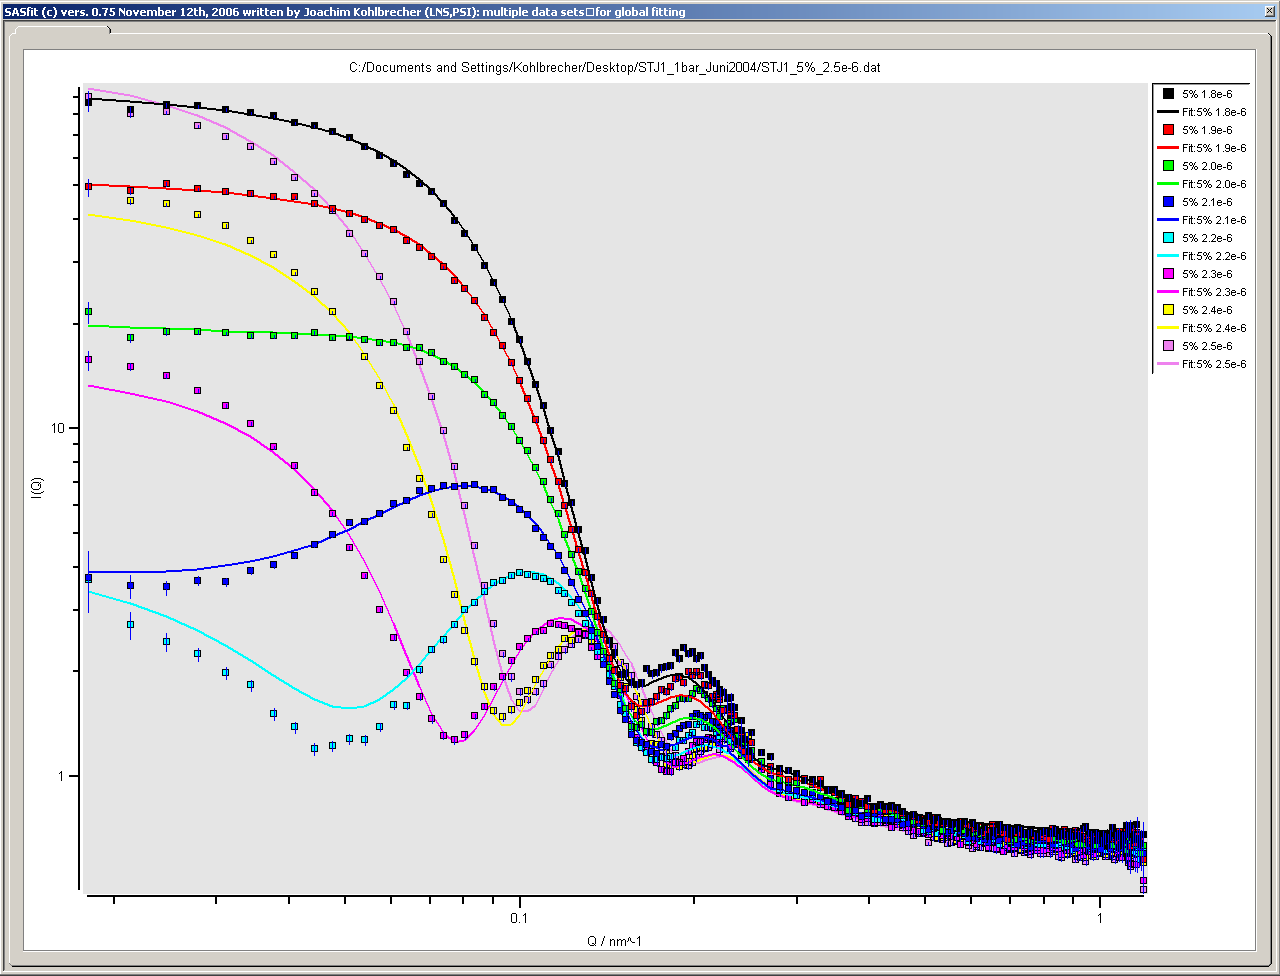
\includegraphics[width=0.9\textwidth,height=0.6\textwidth]{SASfit.png}
\end{center}


\title[SASfit]{{\tt SASfit}: A program for fitting simple
 structural models to small angle scattering data}

\date{\today}

\begin{abstract}
{\tt SASfit} has been written for analyzing and plotting small angle
scattering data. It can calculate integral structural parameters
like radius of gyration, scattering invariant, Porod constant.
Furthermore it can fit size distributions together with several form
factors including different structure factors. Additionally an
algorithm has been implemented, which allows to simultaneously fit
several scattering curves with a common set of (global) parameters.
This last option is especially important in contrast variation
experiments or measurements with polarised neutrons. The global fit
helps to determine fit parameters unambiguously which by analyzing a
single curve would be otherwise strongly correlated. The program has
been written to fulfill the needs at the small angle neutron
scattering facility at PSI (\url{http://kur.web.psi.ch}). The
numerical routines have been written in C whereas the menu interface
has been written in tcl/tk and the plotting routine with the
extension blt. The newest {\tt SASfit} version can be downloaded
from \url{http://kur.web.psi.ch/sans1/SANSSoft/sasfit.html}.
\end{abstract}
\maketitle

\clearpage \tableofcontents
\chapter{Introduction to the data analysis program \SASfit}

Small-angle scattering (SAS) is one of the powerful techniques to
investigate the structure of materials on a mesoscopic length scale
(10 - 10000 {\AA}). It is used to study the shapes and sizes of the
particles dispersed in a homogenous medium. The materials could be a
macromolecule (biological molecule, polymer, micelle, etc) in a
solvent, a precipitate of material A in a matrix of another material
B, a microvoid in certain metal or a magnetic inhomogeneity in a
non-magnetic material. This technique is also used to study the
spatial distribution of particles in a medium, thus providing the
information about the inter-particle interactions. The small angle
scattering methods includes small angle neutron, x-ray or light
scattering. The type of samples that can be studied by scattering
techniques, the sample environment that can be applied, the actual
length scale probed and the information that can be obtained, all
depend on the nature of the radiation employed. The advantage of
small-angle neutron scattering (SANS) over other SAS methods is the
deuteration method. This consists in using deuterium labeled
components in the sample in order to enhance their contrast. Whereas
the disadvantage of SANS over small-angle x-ray scattering (SAXS) is
the intrinsically low flux of neutron sources compared to the orders
of magnitude higher flux at x-ray sources. Neutron scattering in
general is sensitive to fluctuations in the density of nuclei in the
sample. X-ray scattering is sensitive to inhomogeneities in electron
densities whereas light scattering is sensitive to fluctuations in
polarizability (refractive index). In general, irrespective of the
type of radiation, they also share several similarities. Perhaps the
most important of these is the fact that, with minor adjustments to
account for the different types of radiation, the same basic
equations and laws can be used to analyze data from these
techniques. The small-angle scattering data can contain information
concerning both the structure and interaction within the system. This
information can be obtained by either performing model-independent
analysis or detailed model dependent analysis. \SASfit is such a
software package built originally for analysis of small-angle scattering data
in the field of soft matter. The main emphasis of the
software is to provide easy to use graphical user interface.
The software package contains most of
the tools to treat the basic scientific problems for
data produced on a SAS instrument. It allows users to
derive useful information from the SAS scattering data.

\section{Overview}

\SASfit is designed for analysing small angle scattering data and also supplies some simple analysis for dynamic light scattering data. At the moment it performs the following analysis routines to both single 1D data sets as well as multiple 1D data sets, where one like to simultaneously fit several data sets, like from concentration series or contrast variation experiments. In principle by this way also 2D data sets can be analysed by loading segmentationally averaged 2D data.
\begin{itemize}
\item determining integral structural parameters by simple Guinier and Porod analysis
\item fitting and simulating single or multiple data sets in terms of size distribution, form factor and structure factors
\item analysing DLS data in terms of stretched exponentials or cumulants.
\item calculating scattering length densities for x-rays and neutrons
\item solving numerically the Ornstein-Zernike equations for any combination of supplied pair interaction potential and closure relation
\item allows to read, transforms, merge, clip and scale data files. The number of formats is limited.
\end{itemize}
\begin{figure}[htb]
\begin{center}
\
\begin{tikzpicture}
  \path[mindmap,concept color=black,text=white, align=flush center,
    every node/.style=concept]
    node[concept] {\bf \SASfit}
    [clockwise from=90]
    child[concept color=Green,text=white] {
      node[concept] {analytical\ models}
      [clockwise from=112.5, level 2 concept/.append style={sibling angle=45}]
      child[ concept color=LimeGreen ] {
        node[concept] {single\ data set}
        [clockwise from=135 , level 3 concept/.append style={sibling angle=45}]
        child { node[concept color=YellowGreen] {fitting} }
        child { node[concept color=YellowGreen] {simu\-la\-ting} }
      }
      child [ concept color=LimeGreen ] {
        node[concept] {multiple\ data sets}
        [clockwise from=90, level 3 concept/.append style={sibling angle=45}]
        child { node[concept color=YellowGreen] {fitting} }
        child { node[concept color=YellowGreen] {simu\-la\-ting} }
      }
    }
    child[concept color=PineGreen,text=white] { node[concept] {integral\ structural\ parameters}
        [clockwise from=105, level 2 concept/.append style={sibling angle=30}]
        child { node[concept color=ProcessBlue] {Guinier analysis} }
        child { node[concept color=ProcessBlue] {Porod analysis} }
        child { node[concept color=ProcessBlue] {scattering invariant} }
        child { node[concept color=ProcessBlue] {specific surface} }
        child { node[concept color=ProcessBlue] {correlation length} }
        child { node[concept color=ProcessBlue] {etc.} }
    }
    child[concept color=Blue,text=white] { node[concept] {simple DLS analysis} }
%    child[concept color=ProcessBlue] {
%      node[concept] {regu\-la\-ri\-za\-tion tech\-niques (soon)}  }
    child[concept color=Mulberry,text=white] {
      node[concept] {OZ solver}  }
    child[concept color=red,text=white] { node[concept] {IO routines}
        [clockwise from=310, level 2 concept/.append style={sibling angle=30}]
        child { node[concept color=RubineRed] {merging\ scaling\ clipping\ thinning} }
        child { node[concept color=RubineRed] {ALV5000} }
        child { node[concept color=RubineRed] {Clip\-board} }
        child { node[concept color=RubineRed] {SESANS} }
        child { node[concept color=RubineRed] {ASCII} }
        child { node[concept color=RubineRed] {BerSANS} }
        child { node[concept color=RubineRed] {re\-so\-lu\-tion from instr. geom.} }
   }
    child[concept color=BurntOrange,text=black] { node[concept] {SLD\ calculator}
        [clockwise from=-187.5, level 2 concept/.append style={sibling angle=45}]
        child { node[concept color=YellowOrange] {x-rays} }
        child { node[concept color=YellowOrange] {neutrons} }
    };
\end{tikzpicture}
\end{center}
\caption{Mind map about the tools in SASfit}
\label{fig:mindmapSASfit}
\end{figure}


\section{System Requirements And Software Installation}

{\tt SASfit} is a program for analyzing small angle scattering data.
The numerical fitting routines are written in C and the menu
interface in {\tt tcl/tk}. For the plotting of the data the {\tt
tcl} extension {\tt blt} has been used. The last version 0.85 of
{\tt SASfit} has been tested with the {\tt tcl/tk} version 8.3 and
the {\tt blt} version 2.4s. \\

\noindent
\SASfit is available for users analysing data taken at PSI. \\
\SASfit has been developed at the Paul Scherrer Institute (PSI) and remains \copyright\ of PSI. \\
\SASfit is provided to users of the PSI facilities.\\
\SASfit is provided "as is", and with no warranty. \\

\section{Installation Procedure} ~\\

\verb"SASfit" has has been compiled with tcl/tk 8.4 and Blt 2.4. To
install the \texttt{SASfit} package one has to do the following:
\begin{enumerate}
\item Download the zip-file "sasfit.zip" from the \texttt{SASfit}-home page\\
\verb"http://kur.web.psi.ch/sans1/SANSSoft/sasfit.html"
\item extract the contents of the zip file. A new subdirectory called \verb"sasfit" will be generated, which contains all required files.
\item Execute the program  \texttt{./sasfit/sasfit.exe}
\end{enumerate}

\chapter{Quick Start Tour}

\section{User Interface Window}
\begin{figure}[htb]
\begin{subfigure}[b]{.48\textwidth}
   \centering
   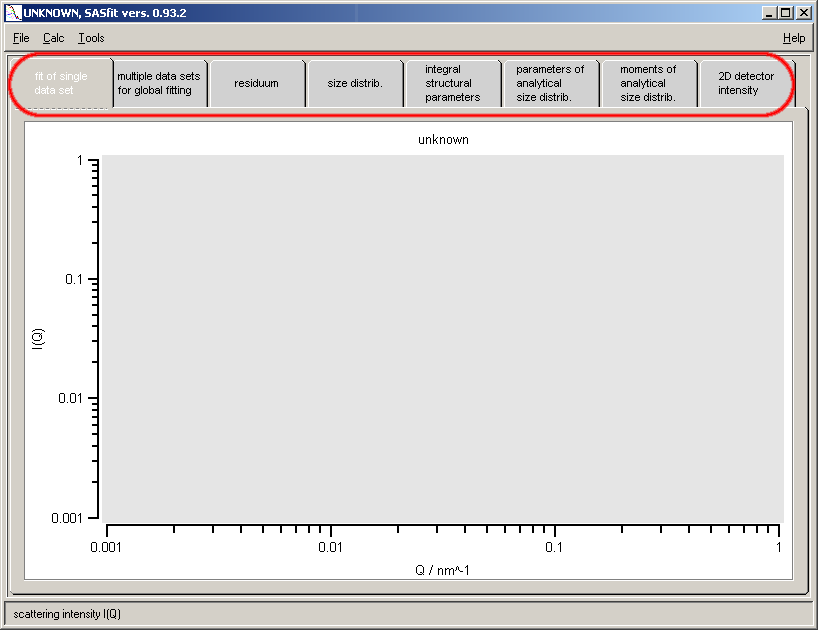
\includegraphics[width=\textwidth]{QTmainA.png}
   \caption{main window}
   \label{fig:QTmainA}
\end{subfigure}
\hfill
\begin{subfigure}[b]{.48\textwidth}
   \centering
   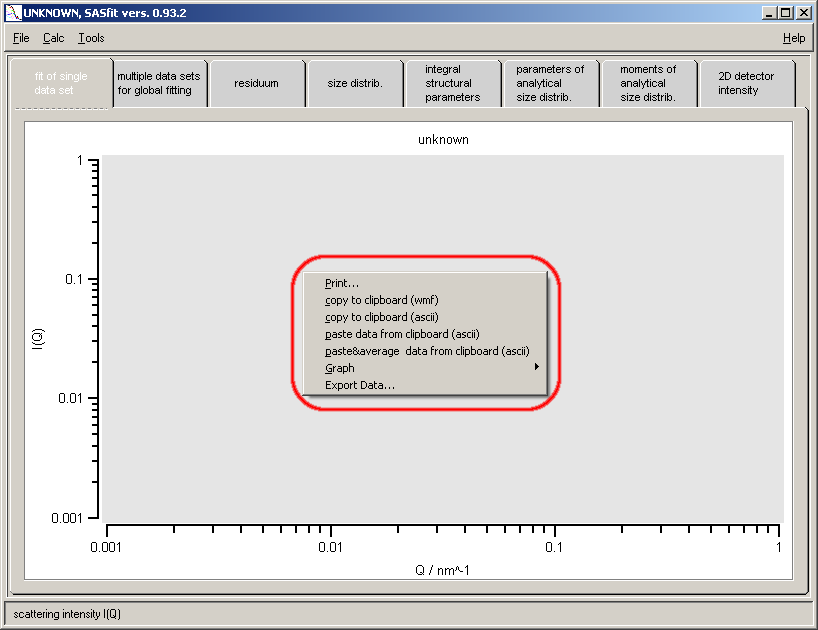
\includegraphics[width=\textwidth]{QTmainB.png}
   \caption{popup menu}
   \label{fig:QTmainB}
\end{subfigure}
\caption{Main \SASfit graphical user interface window}
\label{fig:QTmain}
\end{figure}
\sloppy
The core \SASfit window consists of various tabs (shown in the oval
marking in the figure \ref{fig:QTmainA}, they are "\texttt{fit of single data set}",
"\texttt{multiple data sets for global fitting}", "\texttt{residuum}", "\texttt{size
distrib.}", "\texttt{integral structural parameters}", "\texttt{parameters of
analytical size distrib.}", "\texttt{moments of analytical size
distrib.}", and "\texttt{2D detector intensity}" as shown in the red oval
selection. The tabs for single data set and multiple data sets are used to
plot single or multiple data files and view the plotted graphs along
with the operations to perform during fitting. Residuum shows the
difference between the experimental and theoretical fits. Size
distributions give the plotted view of the number density v/s radius
of the particle. Integral structural parameters are obtained using
model independent fitting, such as Guinier approximation, Porod law
etc. Parameters of analytical size distributions provides with
details of size distributions used and the numbers obtained, whereas
moments of analytical size distribution shows the contribution of
scattering from different size distribution. The final tab 2D
detector intensity is used in case of anisotropic scattering data.
The window were the graphs are generated has options of printing the
graph plotted view, copying the data in the ASCII format or as an
image (wmf) format for further processing or presenting (figure
\ref{fig:QTmainB}). \SASfit accepts the isotropic data in the ASCII
format. The data can be imported as a single data set or for
multiple data sets (several scattering curves).

\section{Importing data files for a single data set}
\begin{figure}[htb]
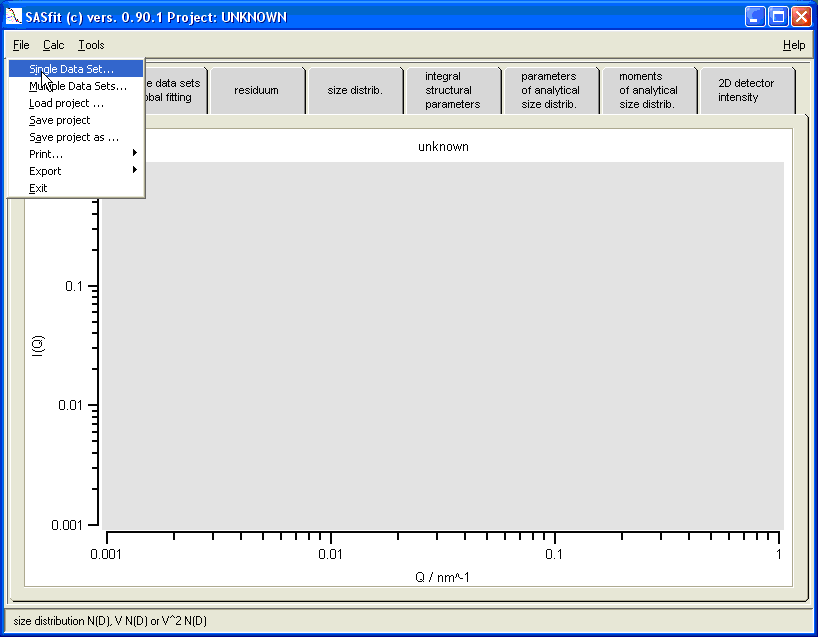
\includegraphics[width=0.48\textwidth]{QTloadingSingleDS.png}
\caption{Menu interface for input single data set}
\label{fig:QTloadingSingleDS}
\end{figure}

\begin{figure}[htb]
\begin{subfigure}[b]{.48\textwidth}
   \centering
    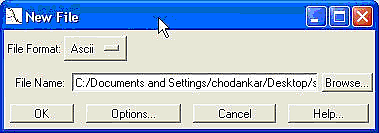
\includegraphics[width=\textwidth]{QTNewFile.png}
   \caption{Path and format selection for new file}
   \label{fig:QTNewFile}
\end{subfigure}
\hfill
\begin{subfigure}[b]{.48\textwidth}
   \centering
   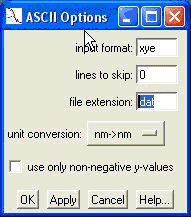
\includegraphics[width=0.48\textwidth]{QTascii1.png} \hfill
   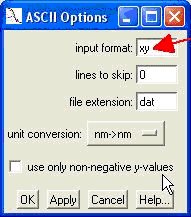
\includegraphics[width=0.48\textwidth]{QTascii2.png}
   \caption{Selecting the format columns of the file}
   \label{fig:QTascii1}
\end{subfigure}
\caption{Importing single data sets} \label{fig:QTNewFileDS}
\end{figure}

The single data set option allows the user to perform operation on a
single data file only. The file is imported via,
\verb"[File|Single Data Set...]" (Figure \ref{fig:QTloadingSingleDS}).
This will open a new file window as shown in figure
\ref{fig:QTNewFile}. The location of the file could be browsed
and respectively selected. The options buttons is supplied to select
the input format, which is performed by supplying a string such as
\texttt{xye}. Where \texttt{x}, \texttt{y} and \texttt{e} stands for
the scattering vector $Q$, scattering intensity $I(Q)$, \texttt{e}
signifies the error bar $\Delta I(Q)$ on the measured scattering intensity.
The error bars are required during the fitting operation and for files
which do not contain the error bar column it would be calculated by
default from the smoothing of the curve. There is an option to skip
lines at the beginning of the data, which is intended to be used to
skip header information in a data file , which could be misinterpreted
as data. The number $n$ specified in the menu defines the number of
lines skipped at the beginning of the data file.
Furthermore a file extension can be provided, unit conversions can be
performed as well as only non-negative $y$-values could be selected
for plotting and performing further analysis. On pressing ok the
data is loaded and the graph is plotted, with a new window labeled
merge files being opened.


\begin{figure}[htb]
\captionsetup[subfigure]{position=b}
\centering
\subcaptionbox{Merge window for merging different $Q$ scales into a single profile\label{fig:QTmergeSDS1}}{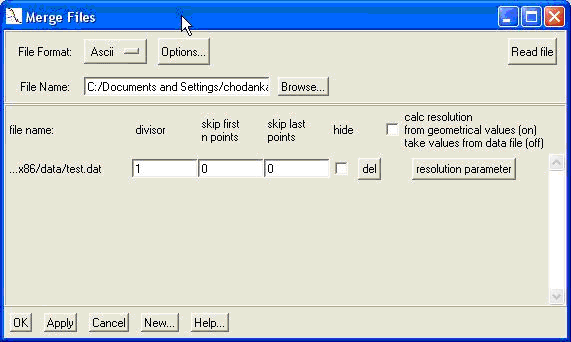
\includegraphics[width=0.47\textwidth]{QTmergeSDS1.png}}
\subcaptionbox{An example showing merged data files\label{fig:QTmergeSDS2}}{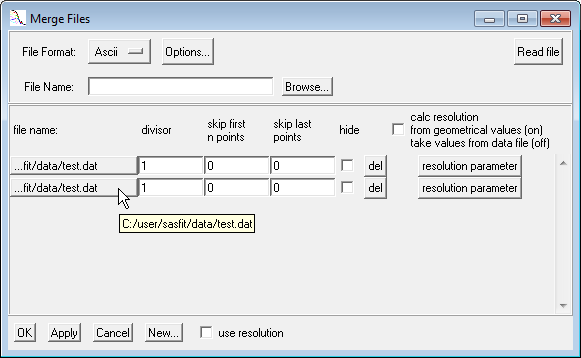
\includegraphics[width=0.47\textwidth]{QTmergeSDS2.png}}
\hfill
\begin{subfigure}[b]{.4\textwidth}
   \centering
   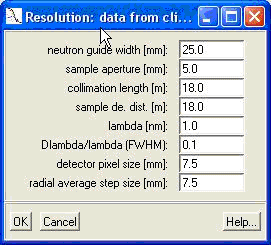
\includegraphics[width=\textwidth]{QTmergeRes.png}
   \caption{resolution parameter interface}
   \label{fig:QTmergeRes}
\end{subfigure}
\caption{Merging many data files to one data set} \label{fig:QTmergeSDScapt}
\end{figure}

In SAS, data can be collected at different collimator and sample to
detector distances to correspond for a wide $Q$ scale. Thus for a
single sample at a given condition there can be more than one data
files, to merge all of them together for completing the scattering
profile, the above shown window comes into play. As shown in the
merge files window, the new file could be browsed and selected; it
has to be read using the read file button. The newly read file
is listed below the first file, if it's a wrong selection it could
be deleted back, also one can scale the different files measured at
different $Q$ windows, using the divisor column to have a continuous
scattering profile. After scaling all the data profiles into one
single profile, the statistically bad and unwanted data points can
be removed by skipping the points at the beginning and at the end of
the data files. The resolution parameters can be provided by
pressing the resolution button and the required information such as
sample to detector distance, collimation distance, cross section of
the guide etc as shown in figure  \ref{fig:QTmergeRes} has to be entered to use
resolution smearing during the fitting. The new button is use to
discard all the current selections and plotted data files and starts
a new session. The file could also be imported by pasting the
clipboard data on the graph view as shown in the figure below. The
conditions for columns are same as that for reading the file via
browse method.


\section{Importing data files for multiple data sets}
\begin{figure}[htb]
\centering
    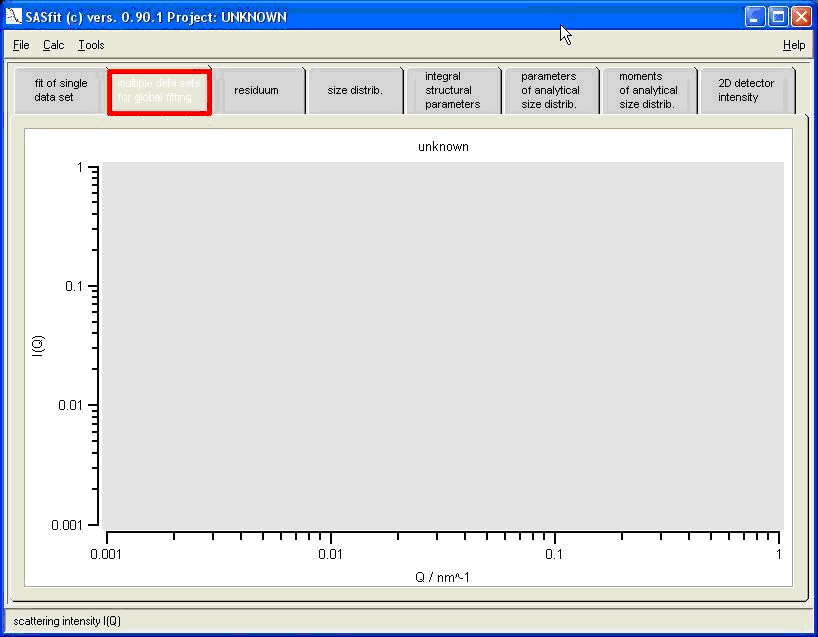
\includegraphics[width=0.48\textwidth]{QTloadingMultipleDS1.png}
    \hfill
    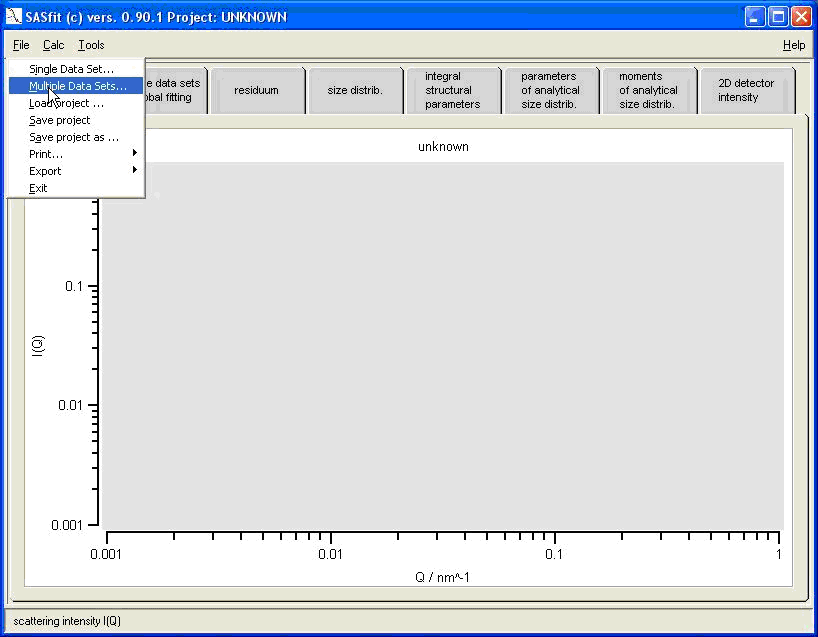
\includegraphics[width=0.48\textwidth]{QTloadingMultipleDS2.png}
\caption{Procedure for importing data files for multiple data sets}
\label{fig:QTmergeMultipleDS1}
\end{figure}
The multiple data set option allows the user to perform operation on
multiple data files by using common set of (global) parameters. This
option is especially important in contrast variation experiments or
measurements with polarized neutrons. The global fit helps to
determine the fit parameters unambiguously which by analyzing a
single curve would be otherwise strongly correlated. The file is
imported by first going to multiple data sets for global fitting
(red box in Figure \ref{fig:QTmergeMultipleDS1}) and then via,
\verb"[File|Multiple Data Set...]". This will open a new window
as was the case for importing single data set
as shown below.
\begin{figure}[htb]
\captionsetup[subfigure]{position=b}
\centering
\subcaptionbox{Path and format selection for new file \label{fig:QTloadingMultipleDS3}}{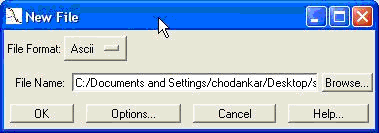
\includegraphics[width=0.6\textwidth]{QTloadingMultipleDS3.png}}
\hfill
\subcaptionbox{Selecting the format of the file \label{fig:QTloadingMultipleDS4}}{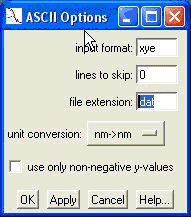
\includegraphics[width=0.3\textwidth]{QTloadingMultipleDS4.png}}
\hfill
\begin{subfigure}[b]{.7\textwidth}
   \centering
   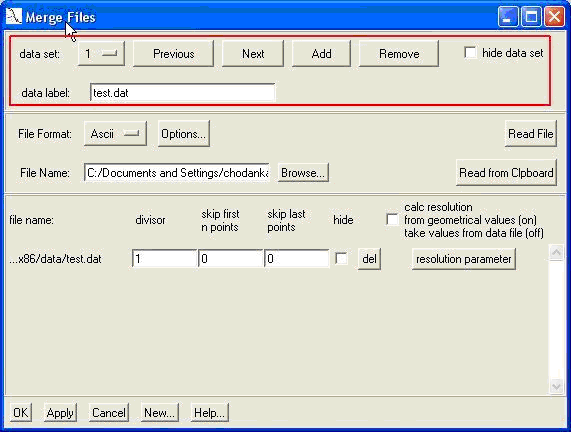
\includegraphics[width=\textwidth]{QTloadingMultipleDS5.png}
   \caption{Merge window for input of multiple data sets. Red box shows the buttons
             from which additional data files could be imported.
             Whereas the features of merging the data set for different $Q$ scales
             is similar to that for importing single data set}
   \label{fig:QTloadingMultipleDS5}
\end{subfigure}
\caption{Procedure for importing data files for multiple data sets}
\label{fig:QTmergeMultipleDS2}
\end{figure}
The procedure for importing the first file is same as was the case
for single file. On reading the first file the merge file window
opens, which has additional buttons as compared to the merge file
window in single data set (shown in the red rectangular box in
figure \ref{fig:QTmergeMultipleDS2}(c)). In multiple data fitting,
almost any number of data files could be loaded. The present active
number of data is shown next to the data set in the merge file
window. One can switch over from one data file to another by
clicking previous or next. Add and remove buttons are used to add or
remove another file. The addition of curves for different $Q$ scales
is performed similar to as mentioned in the Input single data set


\section{Reducing the number of data points}

\SASfit is calculating the intensity for each data point. To make the minimization faster it can be useful to reduce the number of data points. A reduction of data points make sense if they are oversampled, i.e. within the distance of neighbouring q-values the intensity is only changing little. \SASfit supplies two algorithms for reducing the number of data points and one algorithm which is averaging data points.
After reading a data file a new entry is generated in the GUI, see e.\ g.\  \ref{fig:QTmergeMultipleDS2}(c). The filename button activates the GUI (see fig.\ \ref{fig:DataReductionOption}) for choosing an algorithm to reduce optionally the number of data points. Three procedures are supplied at the moment:
\begin{enumerate}
\item averaging neighbouring data points depending on error bar and q difference
\item skipping equally data points to reduce their numbers to a certain percentage
\item skipping nearby data points
\end{enumerate}
 By using the first option an averaging of data points $I_k(q_k) \ldots I_l(q_l)$ is done as long as they fulfill the conditions that
\begin{align}
\forall n \in (k,l] : \abs{I_k-I_n} < D_\mathrm{min} (\Delta I_k + \Delta I_n)
\quad \bigwedge \quad \abs{q_k-q_n}/\overline{q} <  \Delta q_{max}
\end{align}
where $D_\mathrm{min} $ and $\Delta q_{max}$ are user supplied values.
The averaging of data points therefore depends on a user-defined maximum allowed $q$-smearing $\Delta q_{max}$ and  a user-defined maximum distance in intensity in units of the error bar ($D_\mathrm{min} $), so that an averaging is only performed, if the intensities look similar with $D_\mathrm{min}$-times the intensity error bars and are not to far away from each other on the q-axes.
The second option simply skips data points equally to reduce the amount data. The parameter "percentage/100 to load" defines the amount of data to be kept. A value of 1 means all data are kept and a value of 0.5 means every second data point will be kept. In the third option one can define a distance in the $q:I(q)$-plot or $\log q: \log I(q)$ plot. The next data point, which will be plotted must have either in the linear or logarithmic plot a distance exceeding a user defined value.

\begin{figure}[htb]
\captionsetup[subfigure]{position=b}
\centering
\subcaptionbox{Averaging data points depending on the error bar and resulting resolution \label{fig:DataReductionOptionAVG1} }{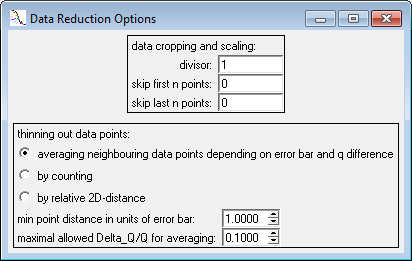
\includegraphics[width=0.32\textwidth]{../images/GUI/DataReductionOptionAVG1.png}}
\hfill
\subcaptionbox{skipping data points to reduce the number of points to a certain amount \label{fig:DataReductionOptionSKIP1} }{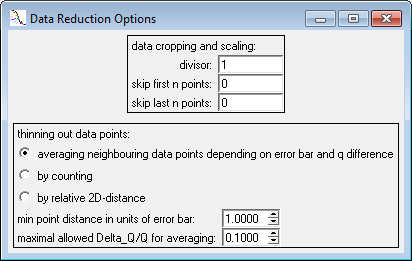
\includegraphics[width=0.32\textwidth]{../images/GUI/DataReductionOptionAVG1.png}}
\hfill
\subcaptionbox{reducing the number of data points by defining a minimum distance between them to be plotted \label{fig:DataReductionOptionSKIP2} }{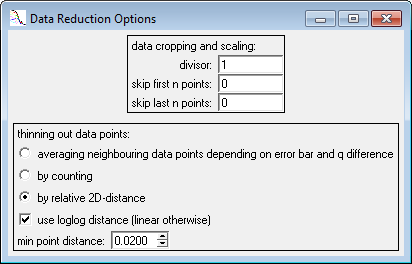
\includegraphics[width=0.32\textwidth]{../images/GUI/DataReductionOptionSKIP2.png}}
\caption{GUI for input values of the two algorithms for reducing the number of data points and for one algorithm which is averaging data points.}
\label{fig:DataReductionOption}
\end{figure}

\section{Simulating scattering curves}

In addition to reading and loading data set, one can also have a
realistic view of the experimental scattering data for a known
structure by simulating the scattering profile beforehand to get a
feel of the actual experiment scattering profile. The simulation can
be performed either for a single data set or for multiple data sets
using global parameters. To generate theoretical scattering profile,
follow \verb"[Calc|Single Data Set...|simulate]" or
\verb"[Calc|Multiple Data Sets...|simulate]", either of them to generate
a single data set or multiple data sets varied by changing the global parameter. The
data can be generated for vast number of form factors and structure
factor included in the software. The simulation is calculated using
physically relevant parameters, this is useful to plan the
experiment and to know whether a given concentration and contrast
would produce a measurable signal.

\begin{figure}[htb]
\begin{subfigure}[b]{.48\textwidth}
   \centering
   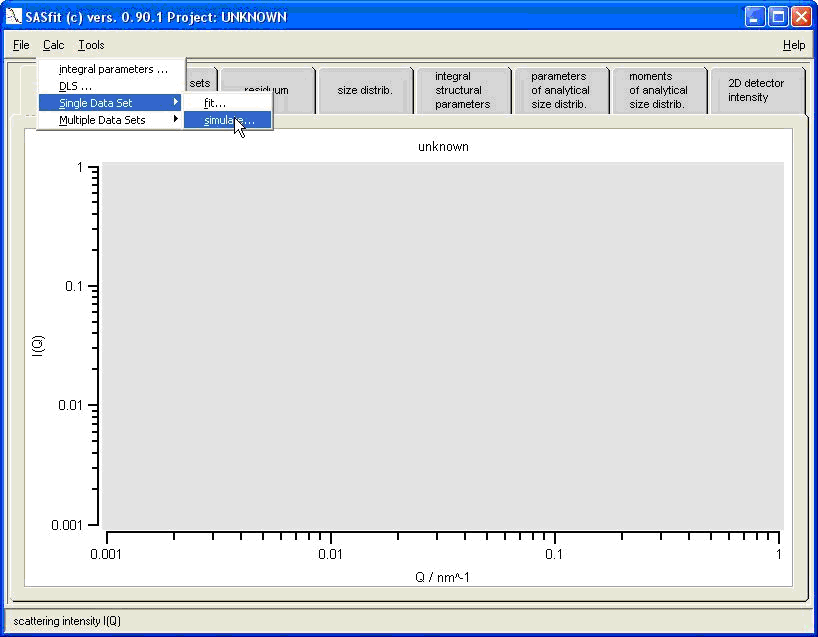
\includegraphics[width=\textwidth]{QTsimulateSDS.png}
   \caption{simulation of a single curve}
   \label{fig:QTsimulateSDS}
\end{subfigure}
\hfill
\begin{subfigure}[b]{0.48\textwidth}
   \centering
   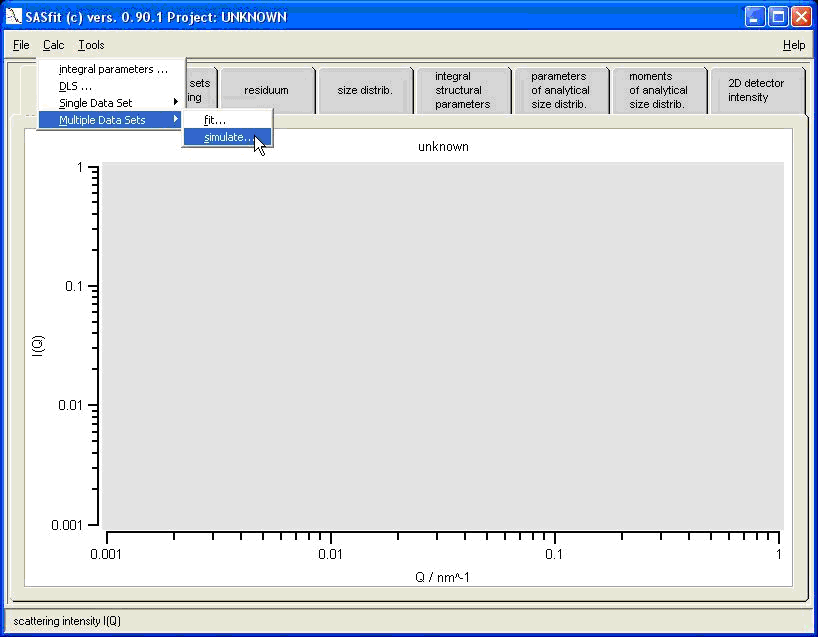
\includegraphics[width=\textwidth]{QTsimulateMDS.png}
   \caption{simulation of multiple curves}
   \label{fig:QTsimulateMDS}
\end{subfigure}
\caption{Procedure for simulating data profiles for single as well as multiple data files}
\label{fig:QTsimulateDS}
\end{figure}

\section{Fitting}
\SASfit can analyse the data using both model-independent analysis
and using a non-linear least square method to fit models. The
model-independent analysis is a preliminary process of analyzing SAS
data and does not require any advanced knowledge of the system to
extract structural information this includes fittings (Guinier,
Kratky, Porod, power-laws, etc.). On the other hand in case of
non-linear least square methods a detailed fitting to the
experimental data is performed using a wide variety of form factors
and structure factors. The \SASfit model library consists of large
number of such functions, which can be readily used for the
analysis. Moreover it can also fit different size distributions.

\subsection{Model Independent Fitting (Integral parameters)} ~\\
Model independent analysis requires no advanced knowledge about the
sample and most importantly no experimental bias of assumed
structure. It includes linearized fitting (Guinier, Porod and Zimm
plot) to extract structural information. Model independent analysis
are performed via \verb"[Cals|integral parameters]". In \SASfit
there are basically three functions available to do the analysis;
they are Guinier, Zimm and Porod approximations (shown in the blue
box in Figure \ref{fig:QTintegralparameter}(b). The number of data points to be included in the
analysis can be accordingly varied and the resulting fit and the
available parameters can be viewed instantaneously. For a large
number of data a small script can be return to automate the process.
This is performed by using the lower section of the integral
structural parameters window (shown in red box). Prename indicates a
character or string of characters with which all the data file names
to be analysed starts with followed by certain numbers. The number
of digits/characters in the filename could be given in the digits
submission box, whereas the start number and the last file number
are provided in their respective submission boxes. The step box
indicates the incremental step of the file names which has to be
analysed. The fitted parameters can be saved in the custom file to
be viewed later. Load next file does step by step analysis of
different files, whereas Do all would perform calculations on the
entire file list, to be saved in the custom file for later viewing.

\begin{figure}[htb]
\centering
\begin{subfigure}[b]{.48\textwidth}
   \centering
   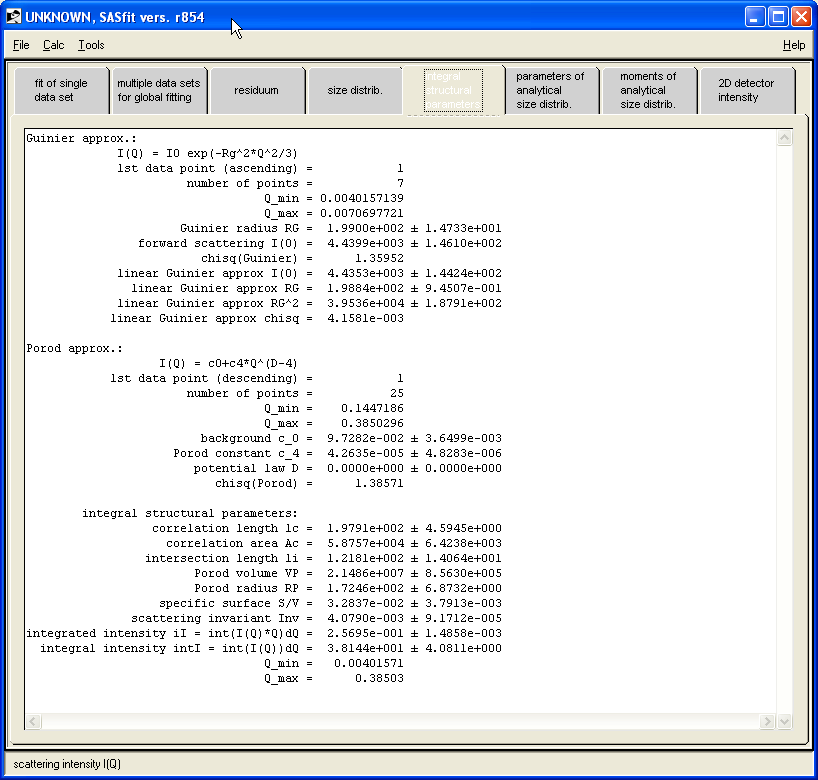
\includegraphics[width=\textwidth]{QTintegralparameterTab.png}
   \caption{data with fit results}
   \label{fig:QTintegralparameterTab}
\end{subfigure}
\hfill
\begin{subfigure}[b]{.48\textwidth}
   \centering
   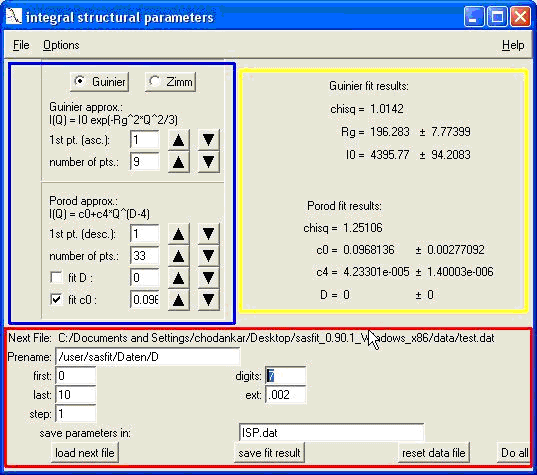
\includegraphics[width=\textwidth]{QTintegralparameterMenu.png}
   \caption{entry menu with fitted parameters}
   \label{fig:QTintegralparameterMenu}
\end{subfigure}
\caption{Integral fit parameters}
\label{fig:QTintegralparameter}
\end{figure}

A set of valuable size and integrated parameters that can be
calculated directly from the scattering curves $I(Q)$
\cite{Damaschun1969,Sjoberg1974,Damaschun1971,Walter1985,Moller1995,book:Guinier:Fournet}
consists of
\begin{subequations}
\begin{align}
\tilde{Q}_\text{inv} &= \int_0^\infty Q^2I(Q) \mathrm{d}Q \mbox{ (scattering invariant)} \\
\frac{S}{V} &= \frac{\pi}{\tilde{Q}_\text{inv}} \;\; {\DS\lim_{Q \to \infty}\left\{Q^4I(Q)\right\}} \mbox{ (specific surface)} \\
\langle R_G \rangle^2 &= 3\left(-\DS\lim_{Q \to 0}\left\{\frac{\mathrm{d}[\ln I(Q)]}{\mathrm{d}(Q^2)}\right\}\right) \mbox{ (squared Guinier radius)} \\
\langle d \rangle &= \frac{4}{\pi}\frac{\int_0^\infty Q^2I(Q) \mathrm{d}Q}{\DS\lim_{Q \to \infty}\left\{Q^4I(Q)\right\}} \mbox{ (average intersection length)} \\
\langle l \rangle &= \frac{\pi}{\tilde{Q}_\text{inv}} \int_0^\infty QI(Q) \mathrm{d}Q \mbox{ (correlation length)} \\
\langle A \rangle &= \frac{2\pi}{\tilde{Q}_\text{inv}}\int_0^\infty I(Q) \mathrm{d}Q \mbox{ (correlation surface)} \\
\langle V \rangle &= \frac{2\pi^2}{\tilde{Q}_\text{inv}} I(0) \mbox{ (correlation volume, Porod volume)}
\end{align}
\end{subequations}

\subsection{Model dependent analysis}
\subsubsection{Modeling a single data set}~\\
\begin{figure}[htb]
\captionsetup[subfigure]{position=b}
\centering
\subcaptionbox{Menu through which fitting procedure is initiated \label{fig:QTsinglefitTab} }{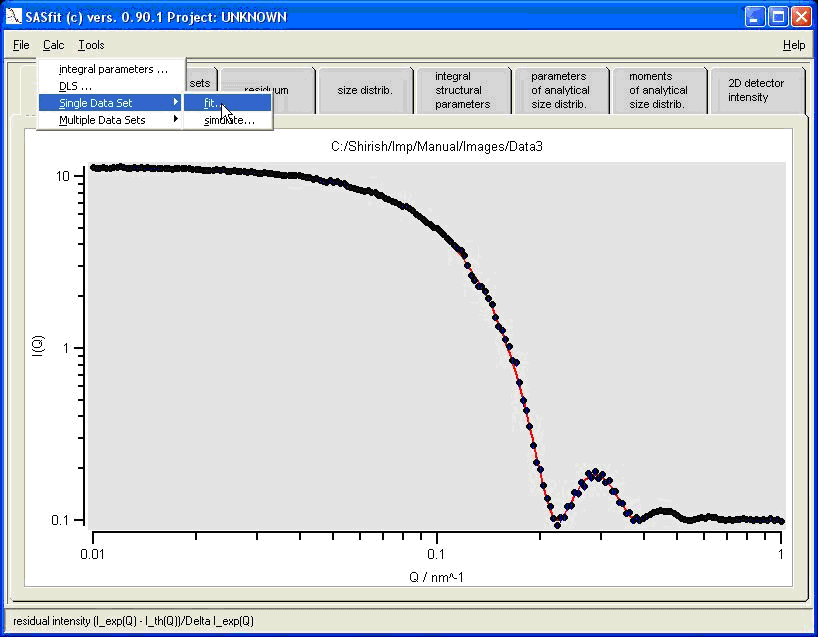
\includegraphics[width=0.5\textwidth]{QTsinglefit1.png}}
\hfill
\subcaptionbox{User interface for fitting, containing different form factors and structure factor \label{fig:QTsinglefitEntryMenu} }{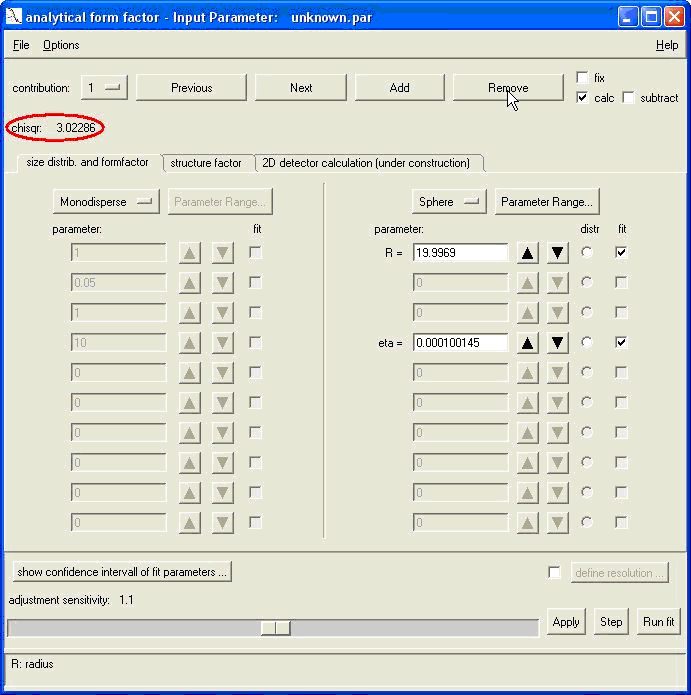
\includegraphics[width=0.48\textwidth]{QTsinglefit2.png}}
\hfill
\subcaptionbox{Tab summarizing the analyzed parameters \label{fig:QTsinglefitParOverview} }{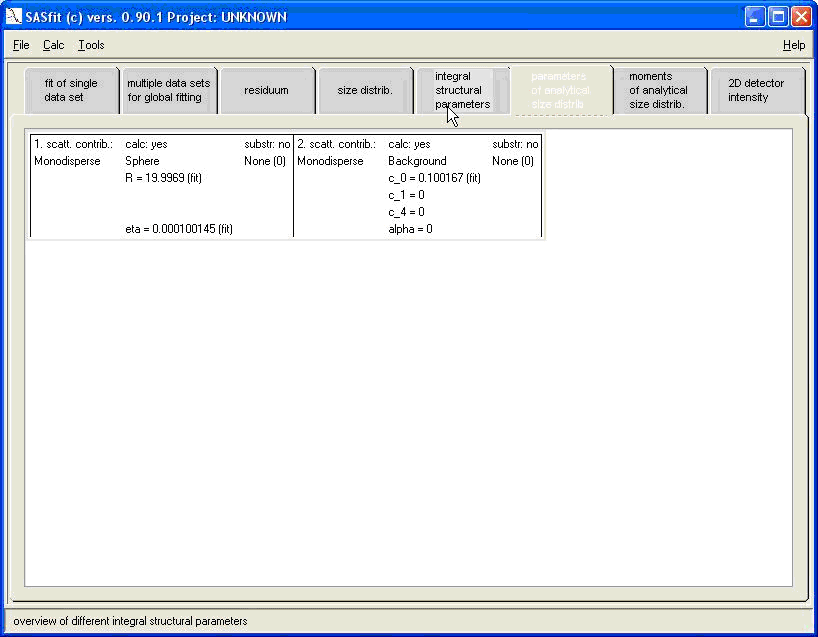
\includegraphics[width=0.48\textwidth]{QTsinglefit3.png}}
\caption{Menus for fitting a single data set}
\label{fig:QTsinglefit}
\end{figure}
For Modeling a SANS data set the \SASfit-programm allows to
describe experimental data with an arbitrary number of scattering
objects types. Each of them can have a size distribution, whereby
the user can choose over which parameter $a_i$ of the form factor
the integration will be performed. For example in case of a
spherical shell with a core radius of $R$ and a shell thickness of
$\Delta R$ \SASfit allows to integrate either over the core
radius $x=R$ or the shell thickness $x=\Delta R$ by marking the
corresponding parameter (see option {\tt distr} in Fig .
\ref{fig:QTsinglefitEntryMenu}). Furthermore an additional structure factor
can be included for each scattering object. Several ways to account
for the structure factor have been implemented like the monodisperse
approximation (\ref{sec:SQmonodisperse}), decoupling approach
(\ref{sec:SQdecoupling}), local monodisperse approximation
(\ref{sec:SQlocalmonodisperse}), partial structure factor
(\ref{sec:SQpartial}) and scaling approximation of partial structure
factors (\ref{sec:SQscaling}). The details are described in chapter
\ref{sec:structurefactor}.

Implemented size distributions, form factors and structure factors
are described in chapters \ref{formfactor},
\ref{sec:structurefactor} and \ref{sizedistribution}. Optional an
additional smearing of this function with the instrument resolution
function $R_{av}\left(Q,\langle Q\rangle\right)$ can be activated so
that
\begin{equation}
I(\langle Q\rangle) = \int_0^\infty R_{av}\left(Q,\langle
Q\rangle\right) \frac{d\sigma}{d\Omega}(Q) \, dQ
\end{equation}

A user interface shown in Fig. \ref{fig:QTsinglefit} is supplied to
choose between the number of scattering objects and to define
parameter for each of them. Next to varying the different parameters
one can mark those to be fixed or fitted (see option {\tt fit} in Fig.
\ref{fig:QTsinglefitEntryMenu}). Model dependent analysis for single files
are performed via \verb"[Calc|Single Data Set|Fit...]".

\subsubsection{Modeling multiple data sets}~\\
\begin{figure}[htb]
\centering
\subcaptionbox{Imported multiple data sets \label{fig:QTmultiplefit1}}{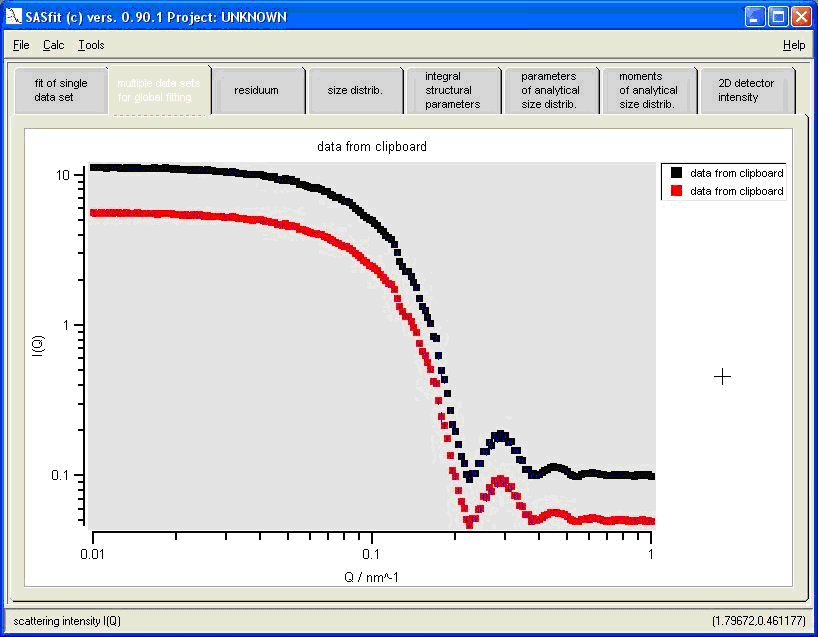
\includegraphics[width=0.48\textwidth]{QTmultiplefit1.png}}
\hfill
\subcaptionbox{User interface for fitting multiple data files \label{fig:QTmultiplefit2} }{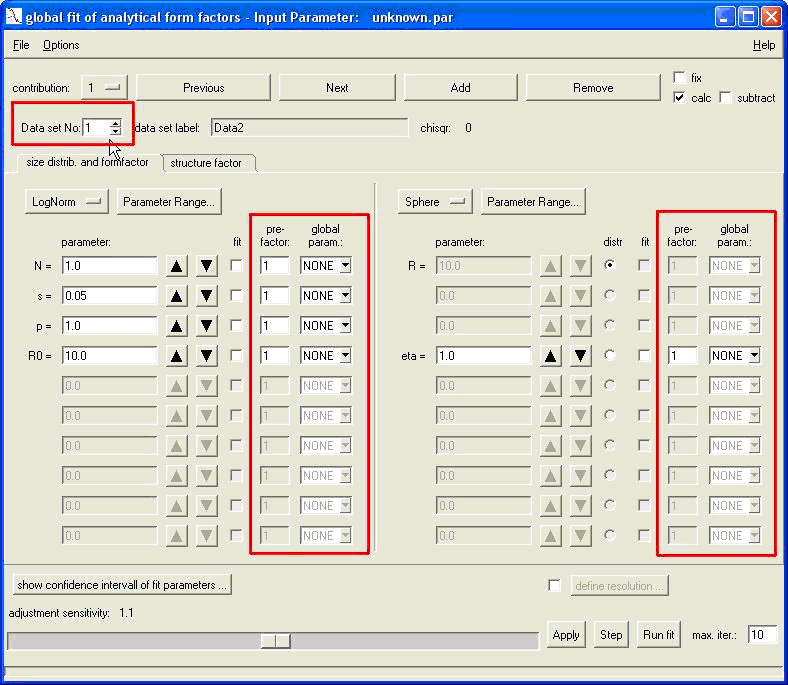
\includegraphics[width=0.48\textwidth]{QTmultiplefit2.png}}
\caption{Menus for fitting a simultaneously multiple data sets}
\label{fig:QTmultiplefit}
\end{figure}
The multiple data set option allows the user to perform operation on
multiple data file by using common set (global) parameters. This
option is especially important in contrast variation experiments or
measurements with polarized neutrons. The global fitting helps the
user to analyse large number of data which has a similar form or
structure factor however different scaling constant. The data shown
in the figure below is for a spherical monodispersed system both the
data profile has identical features, except that the scaling factor
between the two is of a factor of two. The data are called by the
procedure explained in the input multiple data file section. The
fitting of the data is performed by calling the fitting function via
\verb"[Calc|Multiple Data Sets|Fit...]". The user interface for multiple
data fitting has additional feature than to that for single data
fitting, they are pre-factor and global parameters as shown in
figure \ref{fig:QTmultiplefit} red markings.


\begin{figure}[htb]
\centering
\begin{subfigure}[b]{.48\textwidth}
   \centering
   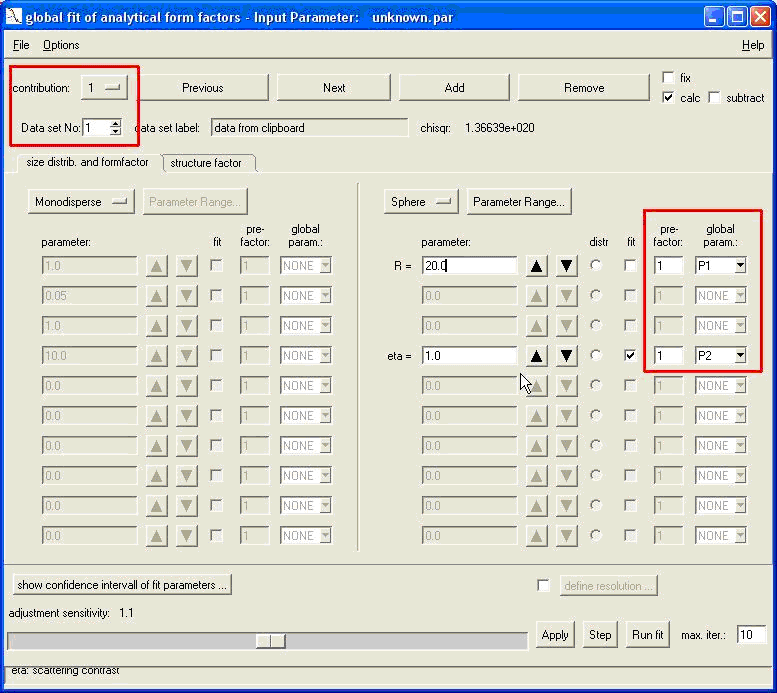
\includegraphics[width=\textwidth]{QTmultiplefitUI1.png}
%   \caption{}
   \label{fig:QTmultiplefitUI1}
\end{subfigure}
\hfill
\begin{subfigure}[b]{.48\textwidth}
   \centering
  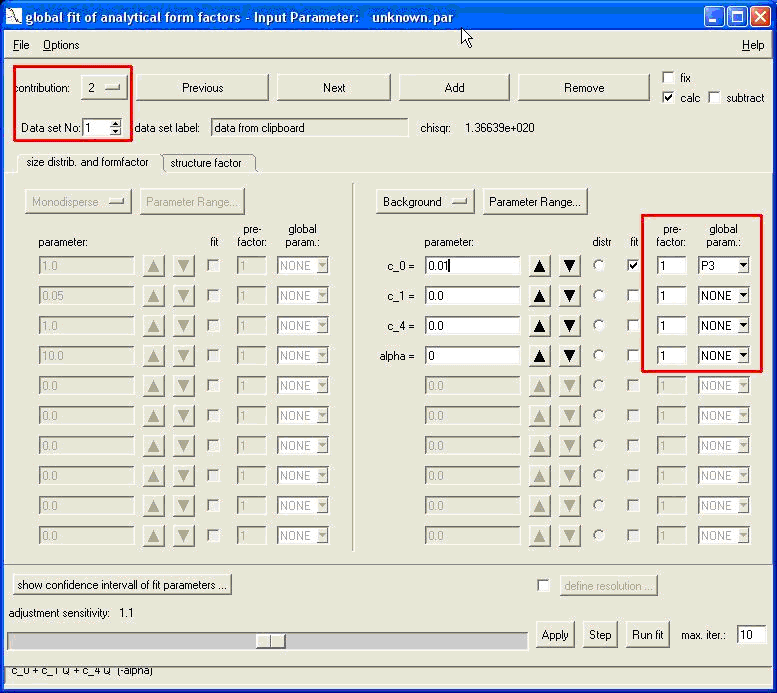
\includegraphics[width=\textwidth]{QTmultiplefitUI2.png}
%   \caption{}
   \label{fig:QTmultiplefitUI2}
\end{subfigure}
\hfill
\begin{subfigure}[b]{.48\textwidth}
   \centering
   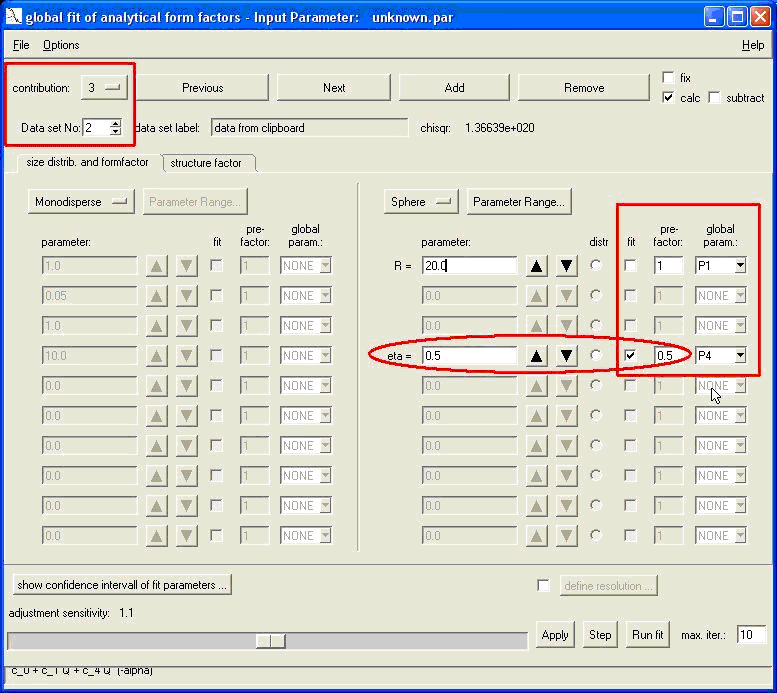
\includegraphics[width=\textwidth]{QTmultiplefitUI3.png}
%   \caption{}
   \label{fig:QTmultiplefitUI3}
\end{subfigure}
\hfill
\begin{subfigure}[b]{.48\textwidth}
   \centering
   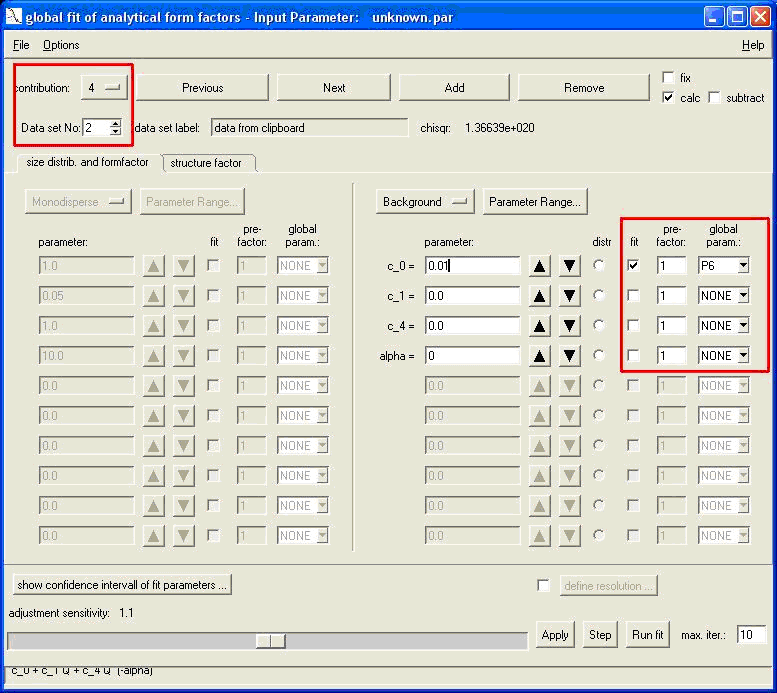
\includegraphics[width=\textwidth]{QTmultiplefitUI4.png}
%   \caption{}
   \label{fig:QTmultiplefitUI4}
\end{subfigure}
\caption{Different windows showing different controlling parameters during multiple data fitting.}
\label{fig:QTmultiplefitUI}
\end{figure}

The procedure for fitting the data set is similar to that mentioned
in the earlier section. The only difference is to include the global
parameters for each function included. The scattering profile shown
in the figure \ref{fig:QTmultiplefit1} is for a spherical
monodispersed particle, both
the profiles have identical features with a scaling factor of two.
The user interface for fitting shows the following window in figures
\ref{fig:QTmultiplefitUI}. The data set number shows the active data file, whereas
contribution indicates the number of scattering objects. We have
selected the form factor for a spherical particle. In the global
parameter a new variable is produced for both radius and \texttt{eta}
(scattering contrast). The pre-factor is kept constant at 1. A
second contribution is added to the data set one by pressing add. In
this case it is a background contribution, a new global parameter is
introduced for it (\texttt{P3}). A similar procedure is done for second data
set where the global parameter for the radius is kept same to that
for data set one, whereas new global parameters are defined for
scattering contrast and background. The fitting procedure can then
be started by pressing Run fit. The figures \ref{fig:QTmultiplefitUIeg}
show the graphs during the fitting process. The parameters of fitting for all the
contribution can be viewed by pressing parameters of analytical size
distributions (figure \ref{fig:QTmultiplefitUIeg4}).

\begin{figure}[htb]
\centering
\begin{subfigure}[b]{.48\textwidth}
   \centering
   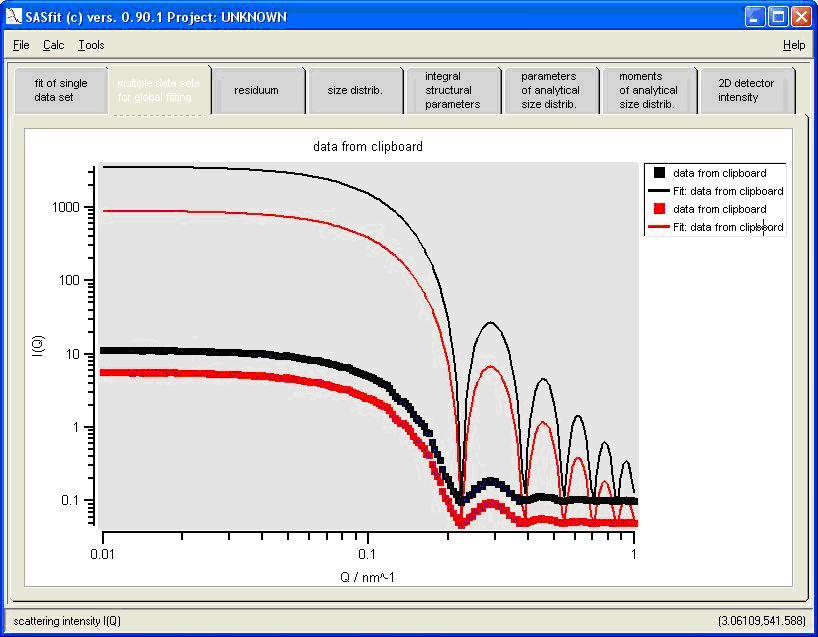
\includegraphics[width=\textwidth]{QTmultiplefitUI5.png}
%   \caption{}
   \label{fig:QTmultiplefitUI5}
\end{subfigure}
\hfill
\begin{subfigure}[b]{.48\textwidth}
   \centering
  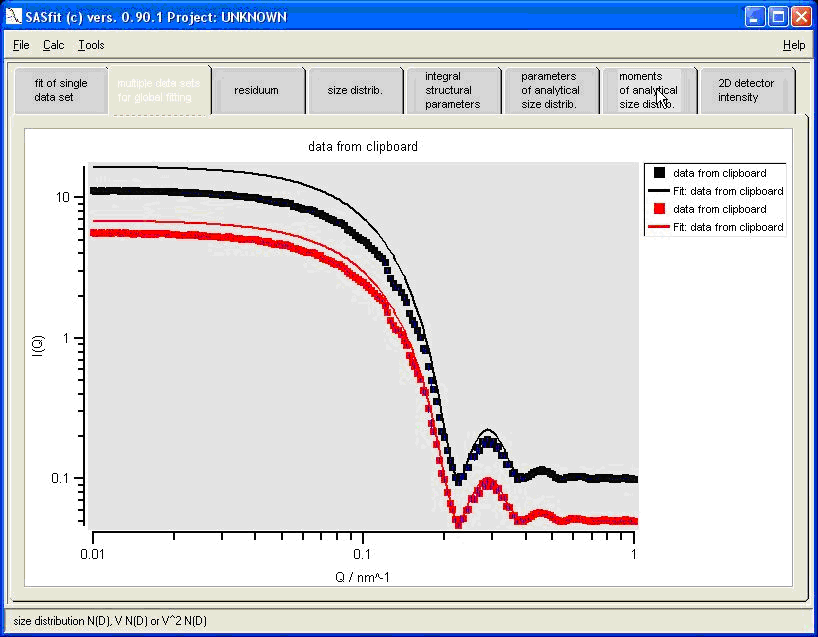
\includegraphics[width=\textwidth]{QTmultiplefitUI6.png}
%   \caption{}
   \label{fig:QTmultiplefitUI6}
\end{subfigure}
\hfill
\begin{subfigure}[b]{.48\textwidth}
   \centering
   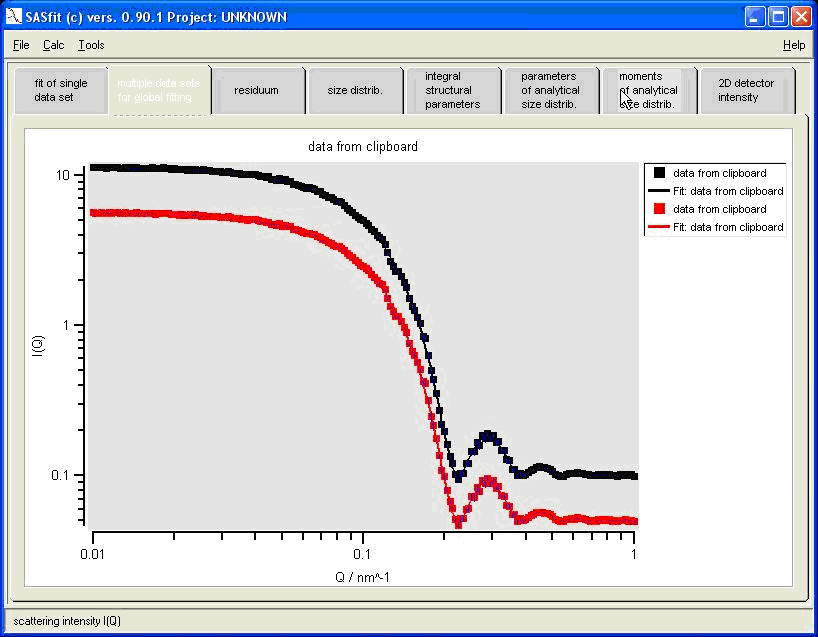
\includegraphics[width=\textwidth]{QTmultiplefitUI7.png}
%   \caption{}
   \label{fig:QTmultiplefitUI7}
\end{subfigure}
\hfill
\begin{subfigure}[b]{.48\textwidth}
   \centering
   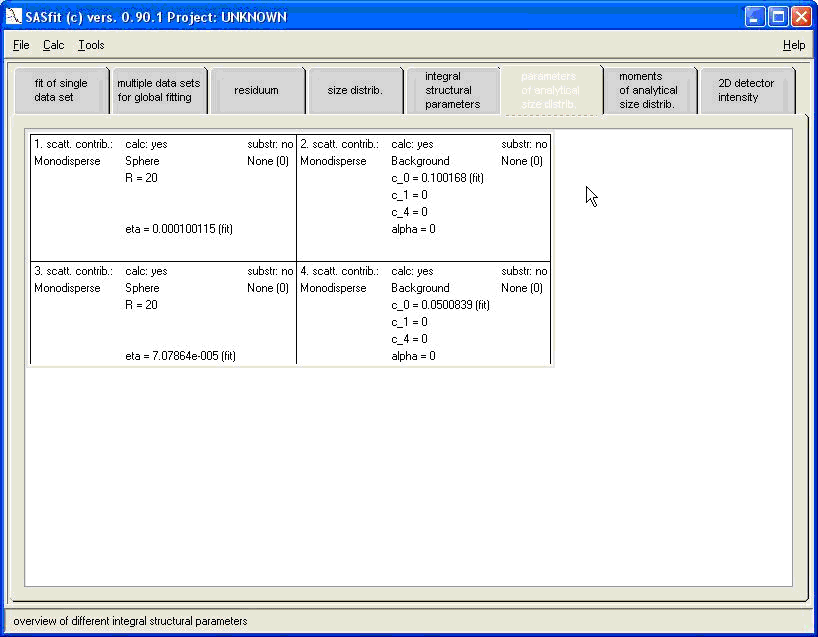
\includegraphics[width=\textwidth]{QTmultiplefitUI8.png}
%   \caption{}
   \label{fig:QTmultiplefitUI8}
\end{subfigure}
\caption{The scattering data profile and the analytical parameters obtained during the fitting process.}
\label{fig:QTmultiplefitUIeg}
\end{figure}


\clearpage
\section{Criteria for goodness-of-fit}
All criteria shown below for testing the goodness of a fit should be
considered with caution \cite{Bevington2003,Press2007}.
When you get data on a SAS instrument
the measured intensities are measured with some statistical uncertainties.
Normally one assumes Poisson statistics to determine the uncertainty
in the counting statistics. The data reduction software should than perform a
proper error propagation analysis for all succeeding data treatment operations.
However, by this procedure only statistical uncertainties are taken into account.
All systematic uncertainties are then hopefully covered during the data treatment,
as for example background correction, transmission correction etc \ref{ch:SASdatacorrection}.
~\\
\subsection{chi square test}
~\\
The method of least squares is built on the hypothesis that the
optimum description of a set of data is one which minimizes the
weighted sum of squares of deviations, between the data,
$I_\text{exp}(q_i)$ , and the fitting function $I_\text{th}(q_i)$:
\begin{equation}
\chi^2 = \displaystyle\sum_{i=1}^N
\left(\frac{I_\text{exp}(q_i)-I_\text{th}(q_i)}{\Delta
I(q_i)}\right)^2
\label{eq:chi2}
\end{equation}
As a rule of thumb for chi-square fitting is the statement that a
good fit is achieved when the reduced chi-square equals one. The
reduced chi-square value, which equals the residual sum of square
divided by the degree of freedom can be computed by
\begin{equation}
\chi^2_\nu = \displaystyle \frac{1}{N-m} \sum_{i=1}^N
\left(\frac{I_\text{exp}(q_i)-I_\text{th}(q_i)}{\Delta
I(q_i)}\right)^2 = \frac{\chi^2}{N-m}
\end{equation}
where $N$ is the number of data points and $m$ the number of fit parameters.
$\nu=N-m$ is called the "number of degree of freedom". The reduced chi-square
is closely related to the variance of the fit $s^2$ by
\begin{equation}
s^2=\chi_\nu^2 \left( \frac{1}{N}\sum_{i=1}^N \frac{1}{\left(\Delta I_i^\text{exp}\right)^2}\right)^{-1}
\end{equation}

In the theory of hypothesis testing $\chi^2$ can be used to test
for goodness of a fit. The probability that a random set of $N$ data points
would yield a value of $\chi^2$ equal or greater than the measured
one is given by
\begin{equation}
\displaystyle Q_\text{factor} =
Q\left(\frac{N-m}{2},\frac{\chi^2}{2}\right) =
\frac{\Gamma\left(\frac{N-m}{2},\frac{\chi^2}{2}\right)}{\Gamma\left(\frac{N-m}{2}\right)}
\text{ with } \Gamma\left(a,x\right) =  \int_x^\infty t^{a-1}e^{-t}
dt
\end{equation}
For a fitting function being a good approximation to the data the experimental
value of $\chi^2_\nu$ should be close to one and the probability
$Q_\text{factor}$ somewhere between 0.01 and 0.5. For probability values
close to one the fit seems to be too good to be true.

\vspace{5mm}

The interpretation of the parameter $Q_\text{factor}$ can be summarized as:

\vspace{5mm}

\uline{\bf goodness-of-fit parameter: $Q_\text{factor}$}
\begin{description}
 \item[$Q_\text{factor}>0.99$] too good
 \item[$Q_\text{factor}>0.1$] believable
 \item[$Q_\text{factor}>0.001$] may be acceptable
 \item[$Q_\text{factor}<0.001$] questionable
\end{description}

\vspace{5mm}

The $Q_\text{factor}$-parameter is calculated after each calculation of the scattering curve together with $\chi^2_\nu$ and $s^2$. They are displayed and updated in the red marked area of the screen shot shown in fig.\ \ref{fig:GoodnessParGUI}.

~\\
\subsection{R-factor}
~\\
The crystallographers have introduced another parameter for the goodness of a fit.
They use the $R$ factor \cite{Rfactor,Hamilton1965} as a measure of model quality which is defined as
\begin{equation}\label{eqRfactor}
  R  \displaystyle  = \frac{\displaystyle\sum_{i=1}^N
\abs{\abs{I_\text{exp}(q_i)} -
\abs{I_\text{th}(q_i)}}}{\displaystyle\sum_{i=1}^N
\abs{I_\text{exp}(q_i)}}
\end{equation}
Theoretical values of $R$ range from zero (perfect
agreement of calculated and observed intensities) to infinity.  $R$
factors greater than 0.5 indicate in crystallography very poor
agreement between observed and calculated intensities. Models
refining to $R < 0.05$ are often considered to be good. However, the
$R$ factor must always be treated with caution, only as an indicator of
precision and not accuracy. In Crystallography partially incorrect
structures have been reported with $R$ values below $0.1$; many
imprecise but essentially correct structures have been reported with
higher $R$ values.

In practice, weighted $R$ factors $R_\text{w}$ are more often used
to track least-squares refinement, since the functions minimized are
weighted according to estimates of the precision of the measured
quantity. The weighted residuals are defined as:
\begin{equation} \displaystyle R_{w} =
\sqrt{\frac{\displaystyle\sum_{i=1}^N \left(\frac{\abs{I_\text{exp}(q_i)}
- \abs{I_\text{th}(q_i)}}{\Delta
I(q_i)}\right)^2}{\displaystyle\sum_{i=1}^N
\frac{I_\text{exp}^2(q_i)}{\Delta I^2(q_i)}}}
\end{equation}


The interpretation of the parameters $R$ and $R_w$ can be summarized as:

\vspace{5mm}

\uline{\bf goodness-of-fit parameters: $R,R_w$}
\begin{description}
\item[$R,R_w>0.3$] questionable
\item[$0.1 > R,R_w >0.3$] may be acceptable
\item[$R,R_w<0.1$] believable
\end{description}

\vspace{5mm}

The parameters $R$ and $R_w$ are calculated like the $Q_\text{factor}$-parameter after each calculation of the scattering curve. They are displayed and updated together with other goodness-of-fit parameters in the red marked area of the screen shot shown in fig.\ \ref{fig:GoodnessParGUI}. The goodness-of-fit parameters are not minimized. The parameter which is minimized is the $\chi^2$-value, defined in eq.\ \ref{eq:chi2}. The other goodness-of-fit parameters are than calculated after each fitting step or after evaluating the theoretical scattering curve via the "Apply"-button.

\subsection{other methods to compare similarity or distance between theory and data}

\begin{itemize}
  \item  \href{https://en.wikipedia.org/wiki/Kullback%E2%80%93Leibler_divergence}{Kullback-Leibler divergency} and  \href{https://en.wikipedia.org/wiki/Jensen%E2%80%93Shannon_divergence}{Jensen–Shannon divergence}
\begin{align}
    D_\mathrm{KL}(P\|Q)&=\sum_{i=1}^np_i\log {\frac{p_i}{q_i}}-p_i+q_i \\
    D_\mathrm{JS}(P\|Q)&=\frac12 D_\mathrm{KL}(P\|Q)+\frac12 D_\mathrm{KL}(Q\|P) \nonumber \\
                       &=\frac12 \sum_{i=1}^n \left(p_i-q_i\right)\left(\log p_i - \log q_i\right)
\end{align}
  \item  \href{https://en.wikipedia.org/wiki/Chi-squared_divergence}{chi-squared divergence}
\begin{align}
    D_{\chi^2}&= \sum_{i=1}^n\frac{\left(p_i-q_i\right)^2}{q_i}
\end{align}
  \item \href{https://en.wikipedia.org/wiki/Hellinger_distance}{Hellinger distance}
\begin{align}
    H(P,Q)&={\frac {1}{\sqrt {2}}}\;{\sqrt {\sum _{i=1}^{k}({\sqrt {p_{i}}}-{\sqrt {q_{i}}})^{2}}}
\end{align}
  \item \href{https://en.wikipedia.org/wiki/Hellinger_distance}{squared Hellinger distance}
\begin{align}
    H^{2}(P,Q)&=1-\sum_{i=1}^{k}{\sqrt {p_{i}q_{i}}}
\end{align}
  \item  \href{https://en.wikipedia.org/wiki/R%C3%A9nyi_entropy#R%C3%A9nyi_divergence}{Rényi divergence of order $\alpha$}:
\begin{align}
    D_{\alpha }(P\|Q)&={\frac {1}{\alpha -1}}\log \left(\sum _{i=1}^{n}{\frac {p_{i}^{\alpha }}{q_{i}^{\alpha -1}}}\right)
\end{align}
    \begin{description}
        \item[$\alpha=0$] $D_{0}(P\|Q)=-\log Q(\{i:p_{i}>0\})$ : minus the log probability under $Q$ that $p_i > 0$
        \item[$\alpha=1/2$] $D_{1/2}(P\|Q)=-2\log \sum_{i=1}^n\sqrt{p_iq_i}$ : minus twice the logarithm of the Bhattacharyya coefficient; (Nielsen \& Boltz (2010))
        \item[$\alpha=1$] $D_{1}(P\|Q)=\sum_{i=1}^np_i\log {\frac{p_i}{q_i}}$ : the Kullback–Leibler divergence;
        \item[$\alpha=2$] $D_{2}(P\|Q)=\log {\Big \langle }{\frac {p_{i}}{q_{i}}}{\Big \rangle }$ : the log of the expected ratio of the probabilities
        \item[$\alpha=\infty$] $D_\infty (P\|Q)=\log \sup_i\frac {p_i}{q_i}$ : the log of the maximum ratio of the probabilities
    \end{description}
  \item \href{https://github.com/stegua/ot1d}{Wasserstein distance} %https://pkomiske.github.io/Wasserstein/ %https://visualstudiomagazine.com/articles/2021/08/16/wasserstein-distance.aspx
  \item \href{https://en.wikipedia.org/wiki/Canberra_distance}{Canberra distance}:
\begin{align}
    D_{CD}&= \sum_{i=1}^n\frac{\abs{p_i-q_i}}{\abs{p_i}+\abs{q_i}}
\end{align}
  \item \href{https://en.wikipedia.org/wiki/Cosine_similarity}{Cosine distance}
\begin{align}
    D_{\cos}&= 1-\frac{\sum_{i=1}^n p_iq_i}{\sqrt{\sum_{i=1}^n p_i^2}\sqrt{\sum_{i=1}^n q_i^2}}
\end{align}

\end{itemize}


\begin{figure}[htb]
\begin{center}
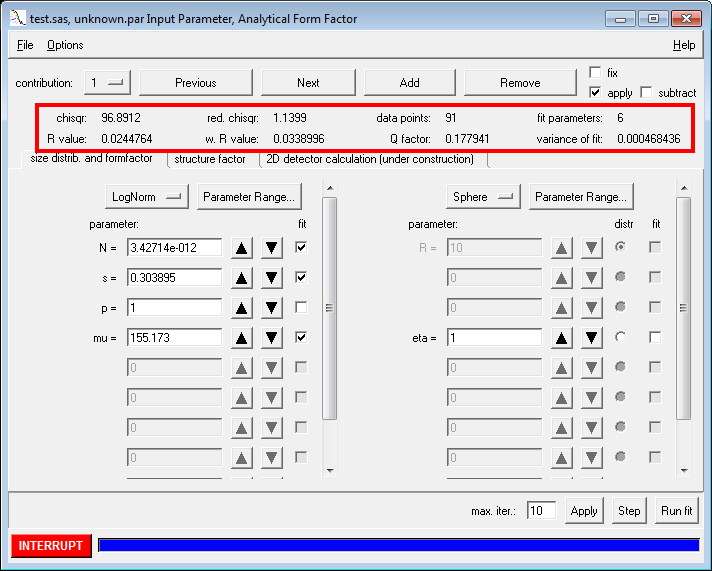
\includegraphics[width=0.712\textwidth]{../images/related_pages/goodnessOFfitPAR.png}
\end{center}
\caption{The parameters $Q, R,R_w$, describing the goodness of the fit, are displayed in the marked area of the GUI}
\label{fig:GoodnessParGUI}
\end{figure}

%~\\
\subsection{Confidence interval of the fitting parameter}
~\\

The confidence intervals of the fitting parameters are calculated at the minimum of the $\chi^2$. At the minimum first the partial derivatives according to the fit parameters $a_i$ are calculated to get the matrix elements $A_{kl}$ via
\begin{align}
A_{kl} &= \sum_{i=1}^{N} \frac{1}{\left(\Delta I_i^\mathrm{th}\right)^2} \frac{\partial I_i^\mathrm{th}(q_i,\mathbf{a})}{\partial a_k} \frac{\partial I_i^\mathrm{th}(q_i,\mathbf{a})}{\partial a_l}
\end{align}
The inversion of this matrix yield the covariance matrix
\begin{align}
        \mathbf{C} &= \mathbf{A}^{-1}
\end{align}
The standard deviations $\Delta a_i$ of the best-fit parameters are given by the square root of the corresponding diagonal elements of the covariance matrix
\begin{align}
\Delta a_i &= \sqrt{C_{ii}}
\end{align}
The correlation coefficient of the fit parameters $a_k$ and $a_l$ are given by
\begin{align}
r_{kl} &= \frac{C_{kl}}{\sqrt{C_{kk}C_{ll}}} = \frac{C_{kl}}{\Delta a_k \Delta a_l}
\end{align}
Both the non-diagonal elements of the correlation matrix $r_{k>l}$ and the confidence intervals of the fitting parameters $\Delta a_k$ are calculated when the fit converges and displayed in a GUI (fig.\ \ref{fig:ErrorGUI}) which can be opened via a menu button as shown in fig.\ \ref{fig:ErrorButton}.

\begin{figure}[htb]
\captionsetup[subfigure]{position=b}
\centering
\subcaptionbox{menu button showing the GUI for the confidence intervals and correlation matrix \label{fig:ErrorButton} }{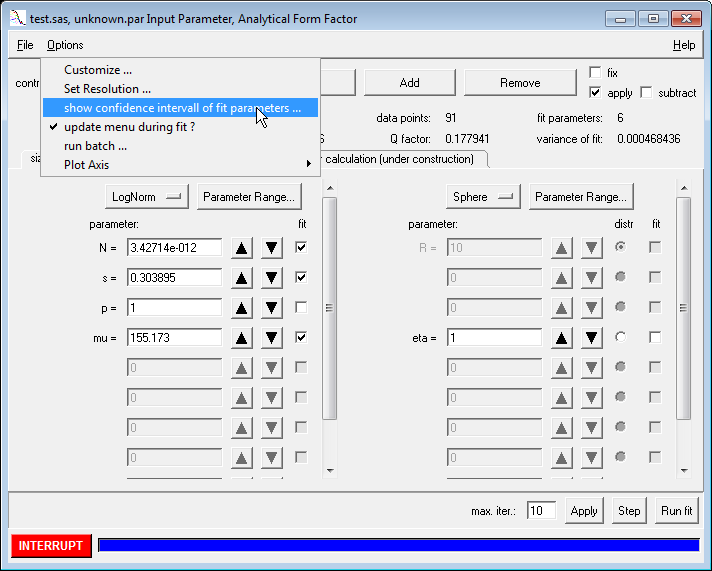
\includegraphics[width=0.47\textwidth]{../images/related_pages/menueConfidenceIntervall.png}}
\hfill
\subcaptionbox{GUI displaying the fitting parameters including confidence intervals and correlation matrix \label{fig:ErrorGUI} }{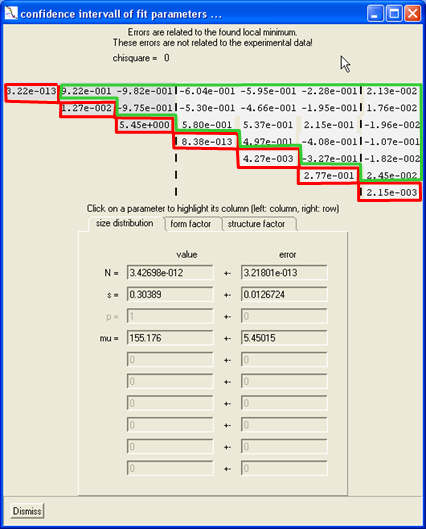
\includegraphics[width=0.47\textwidth]{../images/related_pages/ConfidenceIntervallANDCorrelationMatrix.png}}
\caption{The confidence intervals are calculated at the end of the minimization procedure.}
\label{fig:FitErrors}
\end{figure}

The routine can give nonphysical confidence intervals if
\begin{itemize}
\item no proper error bar for the experimental data are supplied
\item a wrong physical model for describing the data is used
\item the physical model has strongly correlated parameters
\begin{subequations}
\begin{align}
r_{kl} &\approx 0, a_k \mbox{ and } a_l \mbox{ are uncorrelated parameters} \\
r_{kl} &\approx \pm 1, a_k \mbox{ and } a_l \mbox{ are strongly correlated parameters}
\end{align}
\end{subequations}
\end{itemize}

The given value for the confidence interval of the fit parameters should not be used in the cases
\begin{itemize}
\item where the error is not normal distributed
\item where the data is given without error bar
\item where parameters are strongly correlated
\end{itemize}

\clearpage
\section{references to numerical strategies \SASfit make use of}
In small angle scattering analysis numerical integrations tools are used regularly. To get the scattering amplitude a 3D Fourier transform needs to be calculated, which simplifies to lower dimensional integrals in case of point symmetric, spherical symmetric, cylindrical symmetric or planar objects. For non-spherical symmetric shapes typically an average over the orientation distribution needs to be performed. Furthermore for systems with a size distribution an additional smearing over those distributions are essential. For SESANS data a Hankel transformation is required. In case of multiple scattering both a forward and as well as inverse Hankel transform are necessary. It has turned out, that each of these tasks might require a specialized integration routine to be efficient. Efficiency or parallelization becomes in the end essential if several of these integrations have to be solved numerically.

\subsection{Integrals for Form Factors} ~\\

To calculate the general case of a form factor of an object a 3D Fourier transform needs to be performed. When $\eta(\mathbf{r})$ is the scattering length density distribution of the scatterer the scattering amplitude $F(\mathbf{Q})$ is
\begin{align}
F(\mathbf{Q}) &= \int\!\! \int\!\! \int \eta(\mathbf{r}) e^{\imath \mathbf{Q}\mathbf{r}}\,\mathrm{d}\mathbf{r}
\end{align}
For objects with a point symmetric shape the integral simplifies to $\cos$ transform, which is real valued and not anymore complex and for which specialized algorithms are available \cite{Burkardt,Ooura1996,Chase1969,Ooura_1991,Team2024,Team2024a}
\begin{align}
F(\mathbf{Q}) &= \int\!\! \int\!\! \int \eta(\mathbf{r}) \cos\left( \mathbf{Q}\mathbf{r} \right)\,\mathrm{d}\mathbf{r}
\end{align}
For higher symmetric shapes the 3D Fourier transform simplifies further to lower dimensional integrals.

For spherical symmetric shapes one just needs to calculate
\begin{align}
F(Q) &= \int_0^\infty 4\pi r^2 \eta(r) \frac{\sin \left(Qr \right)}{Qr} \, \mathrm{d}r
\end{align}
which now only depend on the modulus of $Q$ and $r$. In this case a $\sin$ transform needs to be calculated. In all cases the integral has to be performed over an oscillating $\cos$ or $\sin$ function, which in the above two cases also have a constant oscillation frequency. Efficient algorithms can be found e.g. at \cite{Burkardt,Ooura1996,Chase1969,Ooura_1991,Team2024,Team2024a}

For cylindrical and point symmetric objects the Fourier transform reads as
\begin{align}
F(\mathbf{Q}) &= 2\pi\int_{-\infty}^{\infty}\cos(Q_zz) \int_0^\infty
\Delta\eta_\textrm{cyl}(r,z) \textrm{J}_0(Q_rr)r \,
\textrm{d}r \textrm{d}z
\end{align}
The integration over $z$ is still a $\cos$ transform, whereas the integration over the other two direction turn into a Hankel transform. The Bessel function also oscillates around zero but not with a fixed frequency. The roots are not analytically known which means some additional efforts for numerically evaluating them. The form factor of a homogeneous cylinder of length $L$ and radius $R$ oriented with the cylinder axis in $z$-direction therefore reads as
\begin{subequations}
\begin{align}
F_\mathrm{cyl}(\mathbf{Q}) &= 2\pi\int_{-L/2}^{L/2}\cos(Q_zz) \int_0^R
 \textrm{J}_0(Q_rr)r \,
\textrm{d}r \textrm{d}z \label{eq:FcosHankel}\\
&= \frac{\sin(Q_zL/2)}{Q_zL/2} \pi R^2L\frac{2\textrm{J}_1(Q_rR)}{Q_rR}  \label{eq:FcylOriented}
\end{align}
with
\begin{align}
\mathbf{Q} &= \begin{pmatrix}
                 Q_r \cos(\phi) \\
                 Q_r \sin(\phi) \\
                 Q_z \\
               \end{pmatrix}
\end{align}
\end{subequations}
In case of a homogeneous cylinder the $\cos$ and Hankel transform can be calculated analytically. For other more realistic models the integrations needs to be performed numerically. Algorithms for the $\cos$ transform already have been mentioned. For the Hankel transform several strategies have been discussed and used \cite{Chave1983,Anderson1989,Ooura_1991,Guptasarma1997,Ogata2005,Kong2007,Key2012,Kang2021}
From these algorithms especially the one from \cite{Ooura_1991} and \cite{Chave1983} are those which  both are fast as well as able to perform the transform with a given precision. The integral in eq.\ \ref{eq:FcosHankel} likely would gain using different quadrature strategies for $\int\mathrm{d}r$ (optimized Hankel transform quadrature \cite{Chave1983}) and $\int\mathrm{d}z$ (e.g.\ double exponential quadrature \cite{Mori2001,Mori1990}), i.e.\ a quadrature rule from a product of distinct optimum 1D quadrature rules needs to be investigated.

\subsection{Orientational and Size Distribution} ~\\

To calculate scattering pattern of particles with orientational (o) and size distribution (s) the scattering intensity $I=\langle \vert F\vert^2\rangle_\mathrm{o,s}$ has to averaged in case of non interacting particles. $\langle \rangle_\mathrm{o,s}$ denotes a multiple quadrature over the orientation and size probability function. In case of interacting particles both the averages of scattering intensities $I=\langle \vert F\vert^2\rangle_\mathrm{o,s}$ of a single particle  as well as the averages of the scattering amplitude $\vert\langle F\rangle_\mathrm{o,s}\vert^2$ of them are typically required.

In case of an averaged amplitude $\langle F\rangle_\mathrm{o,s}$ the integrals over a 3D hyper cube can be extended to the required $n$-dimensional hypercube including orientational as well size distribution. The orientational distribution increases the dimension of the hyper cube by maximal 3 dimensions namely the three Euler angles. Distributions of the size can in principle have any number of dimensions depending on the parametrization. A three dimensional rectangular cuboidal multi shell can have many size parameters in its form factor, each having a distribution.

In contrast to the calculation of the average amplitude the calculating of the averaged intensity first needs a $\vert F(\mathbf{Q})\vert^2$ operation which avoids extending directly the strategies  for quadrature algorithms over a hyper cube to higher dimensions.
Size distribution and orientation distributions over $m$ parameters $a_i$ (with $\mathbf{a}=(a_1, \ldots, a_m)^T$) and over the Euler angles  $(\alpha,\beta,\gamma)$ with a common distribution $p(\mathbf{a},\alpha,\beta,\gamma)$ of the form factor are simply calculated by
\begin{multline} \label{eq:Fredholm}
 \frac{d\sigma(\mathbf{Q})}{d\Omega} = I(Q) = \left\langle \vert F(\mathbf{Q},\mathbf{a},\alpha,\beta,\gamma)\vert^2\right\rangle_{\mathrm{o},\mathrm{s}} = \\
 \idotsint  p(\mathbf{a},\alpha,\beta,\gamma) \vert F(\mathbf{Q},\mathbf{a},\alpha,\beta,\gamma)\vert^2 \, \mathrm{d}\mathbf{a} \, \mathrm{d}\alpha \, \mathrm{d}\beta \, \mathrm{d}\gamma
\end{multline}
The determination of the distribution function $p(\mathbf{a},\alpha,\beta,\gamma)$ is one of the core tasks in small angle scattering analysis. The integral in eq.\ \ref{eq:Fredholm} is a multidimensional Fredholm integral. The SASview as well SASfit packages try to solve this (ill-posed) integral equation by assuming analytical parametrized distribution functions to obtain the orientation and size distribution information. In many typical cases discussed in literature a size and  orientation distributions are assumed to be factorizable as
\begin{align}
p(\mathbf{a},\alpha,\beta,\gamma) &= p_\mathrm{o}(\alpha,\beta,\gamma)\prod_{i=1}^m p_{\mathrm{s},i}(a_i)
\end{align}
where the size distribution $p_{\mathrm{s},i}(a_i)$ is described in first approximation by a simple distribution function like a normal, lognorm, gamma, ... distribution and $p_\mathrm{o}(\alpha,\beta,\gamma)$ is describing the orientation distribution function in terms of Euler angles.


For cylindrical symmetric objects due to symmetry one integration around the symmetry axis can be done analytically, whereas the other two over the polar angles still might need to be performed numerically.
For integration over polar angles, i.e. over the surface of a unit sphere special algorithms are available like Lebedev quadrature \cite{Lebedev1975,Lebedev1976,Lebedev1977,Lebedev2003}, spherical designs \cite{Graef2011,Hardin1996}, or spherical Fibonacci point sets \cite{Marques_2013,Swinbank2006}. However, these methods have the disadvantage of having no error estimate of the integral, but on the other side they might be easily adapted for parallelization due to the known grid points.

A special case of orientation distribution is the fully random orientation distribution. For this case all direction between the scattering object and the vector $\mathbf{Q}$ are equal probable and an average over all direction of $\mathbf{Q}$ is equivalent to averaging over all 3 Euler angles. This means, that a random orientational average requires again an integration over a unit sphere. A symmetry constrain like a cylindrical symmetry of the particles would reduce the orientation average to a single integral. In case of a random oriented cylinder like in eq.\ \ref{eq:FcylOriented} the average reads as
\begin{multline}\label{eq.Fcyl_rndODF}
\vert\left\langle F_\mathrm{cyl}(\mathbf{Q})\vert^2\right\rangle_{\mathrm{rnd-o}} = \\
\int_0^{\pi/2} \left\vert \pi R^2L \frac{\sin(QL/2\cos(\theta))}{QL/2\cos(\theta)} \frac{2\textrm{J}_1(QR\sin(\theta))}{QR\sin(\theta)}\right\vert^2 \sin(\theta) \, \mathrm{d}\theta  \end{multline}
The kernel of this integral is an oscillating function, but it does not oscillate around zero as the kernel is strictly positive. Therefore certain integration strategies for oscillating functions can not be applied directly. We also have two oscillations, one depending on the length $QL/2$ and the other on $QR$. If the cylinder has additional size distributions in $L$ and $R$ the final multidimensional integral to be solved is
\begin{multline}\label{eq.Fcyl_rndODF}
\frac{d\sigma_{\mathrm{cyl},\mathrm{rnd-o},\mathrm{s}}(Q)}{d\Omega}=\left\langle \vert F_\mathrm{cyl}(\mathbf{Q})\vert^2\right\rangle_{\mathrm{rnd-o},\mathrm{s}} = \int_0^\infty \!\int_0^\infty \!\int_0^{\pi/2} p_\mathrm{s}(L,R) \quad \times\\
 \left\vert \pi R^2L \frac{\sin(QL/2\cos(\theta))}{QL/2\cos(\theta)} \frac{2\textrm{J}_1(QR\sin(\theta))}{QR\sin(\theta)}\right\vert^2 \sin(\theta) \, \mathrm{d}\theta  \, \mathrm{d}R\, \mathrm{d}L
\end{multline}
The integral kernel behaves well enough so that the order of the integrals can be changed. If the orientational average is done first, the resulting function in this case for $2R\approx L$ does not has anymore many oscillations and the outer integrations over $L$ and $R$ might be done easily with standard strategies for quadratures over hypercubes. However, for extreme aspect ratios this is not anymore valid.

\subsection{SESANS - MSAS - resolution function} ~\\
\subsubsection{SESANS} ~\\
In case of an isotropic scatterer the SESANS signal $\tilde{G}(\delta)$ is directly related to the SANS differential cross-section $\frac{d\sigma(Q)}{d\Omega}$ via a zero order Hankel transform \cite{Krouglov2003,Andersson2008,Kohlbrecher2017}which reads as
\begin{align}
\tilde{G}(\delta) &= \frac{1}{2\pi}\mathcal{H}_0\left[\frac{\mathrm{d}\sigma(Q)}{\mathrm{d}\Omega}\right](\delta)
= \frac{1}{2\pi} \int_{0}^{\infty} Q J_0(Q\delta) \frac{\mathrm{d}\sigma(Q)}{\mathrm{d}\Omega} \, \mathrm{d}Q
\end{align}
Coming back to the example of random oriented cylinders with size distributions for the length and radius we finally end up with
\begin{multline}  \label{eq.Fcyl_rndODF_SESANS}
\tilde{G}_{\mathrm{cyl},\mathrm{rnd-o},\mathrm{s}}(\delta) = \frac{1}{2\pi} \int_{0}^{q_\mathrm{max}} \! \int_0^\infty \!\int_0^\infty \!\int_0^{\pi/2} Q J_0(Q\delta) \, p_\mathrm{s}(L,R) \quad \times\\
 \left\vert \pi R^2L \frac{\sin(QL/2\cos(\theta))}{QL/2\cos(\theta)} \frac{2\textrm{J}_1(QR\sin(\theta))}{QR\sin(\theta)}\right\vert^2 \sin(\theta) \, \mathrm{d}\theta  \, \mathrm{d}R\, \mathrm{d}L \, \mathrm{d}Q
\end{multline}
As experimentally SESANS signals are only measured with a detector probing the polarization to a maximum value of $q_\mathrm{max}$, the Hankel transform might be significantly truncated. If in this case $\int_{0}^{q_\mathrm{max}} \mathrm{d}Q$ can be replaced by $\int_{0}^{\infty} \mathrm{d}Q-\int_{q_\mathrm{max}}^\infty \mathrm{d}Q$ or if a another routine preferable directly evaluates the integral  $\int_{0}^{q_\mathrm{max}} \mathrm{d}Q$ might depend on how many roots of the Bessel function are within the domain $[0,q_\mathrm{max}]$.

\subsubsection{Multiple Small Angle Scattering (MSAS)} ~\\

According to \cite{Schelten1980,Jensen2018} multiple  small angle scattering can be computed from the single scattering approximation via the intermediate function $i_1(r)$.
\begin{align}\label{eq:MSAS_SchmatzSchelten}
 i_1(r) &= 2\pi t \int_0^\infty J_0(qr) \frac{\mathrm{d}\sigma_1}{\mathrm{d}\Omega}(q) q \mathrm{d}q \\
 &=2\pi t \mathcal{H}_0\left[\frac{\mathrm{d}\sigma_1}{\mathrm{d}\Omega}(q)\right](r)= 4\pi^2 t \tilde{G}(r)\\
 i_m(r) &= e^{-i_1(0)/k_0^2}k_0^2\left(\exp\left(i_1(r)/k_0^2\right)-1\right) \\
        &= k_0^2\left[\exp\left(\frac{t}{k_0^2}\left(\tilde{G}(r)-\tilde{G}(0)\right)\right)-\exp\left(-\frac{t}{k_0^2}\tilde{G}(0)\right)\right] \label{eq:MSASim}\\
 \frac{\mathrm{d}\sigma_m}{\mathrm{d}\Omega}(q)&= \frac{1}{2\pi t} \int_0^\infty J_0(qr) i_m(r) r \mathrm{d}r = \frac{1}{2\pi t} \mathcal{H}_0\left[i_m(r)\right](q) \label{eq:MSAS}\\
 k_0 &= \frac{2\pi}{\lambda}
\end{align}
where $\frac{\mathrm{d}\sigma_m}{\mathrm{d}\Omega}(q)$ is the measured scattering cross-section including multiple scattering contributions normalized on the sample volume and  corrected for absorption and incoherent scattering, i.e. corrected for all beam attenuation effects except coherent small angle scattering. $\frac{\mathrm{d}\sigma_1}{\mathrm{d}\Omega}(q)$ is the corresponding single scattering cross-section per volume.
It can be seen, that the intermediate function $i_1(r)$ is except a pre-factor identical to the projected correlation function $\tilde{G}(r)$ used in the theory of  SESANS analysis,
$i_1(r)=\tilde{G}(r)\left(2\pi\right)^2t$.

What does this mean for the case of random oriented cylinders with a size distribution for the length and radius? Here we consider a system which would scatter that strong, that multiple scattering has to be considered. In this case first the correlation function in eq.\ \ref{eq.Fcyl_rndODF_SESANS} and afterwards the intermediate function including multiple scattering $i_m(r)$ is calculated. This functions then needs to be Hankel transformed again according to eq.\ \ref{eq:MSAS}. In total 5 nested numerical integration are required for the example of polydisperse random oriented cylinders.

%In the \texttt{SASfit} C-source code a function \texttt{sasfit\_hankel()} is supplied to perform a
%Hankel transform. It can be configured to use several different algorithms:
%\cite{Chave1983,Anderson1989,Ooura_1991,Guptasarma1997,Ogata2005,Kong2007,Key2012,Kang2021}
%From these algorithms especially the one from \cite{Ooura_1991} and \cite{Chave1983} are those which
%are both fast as well as able to perform the transform with a given precision.

%It would be interesting to compare those algorithm against newer ones, e.g.
%\cite{Liu2024,Xu2019,Diehl2024,Diehl2024a} for converting SANS cross sections into a SESANS intensity.

\subsubsection{Resolution Function} ~\\
If the resolution function needs to be included in the analysis eq.\ \ref{eq:MSAS} or eq.\ \ref{eq.Fcyl_rndODF} would need to be convoluted by a resolution function which would add another integral to the formula.

\subsection{Summary} ~\\

Already for a simple model of a polydisperse random oriented cylinder several nested integrals needs to be solved numerically.
A part of the integrals, like over a combined orientation and size distribution are calculated over a hyper cube. Adaptive algorithms have been discussed and supplied in \cite{Johnson2017,Genz1980,Berntsen1991,Bull1995}. However, in the present case integrals in certain dimensions might profit if they would be treated with different strategies, like Hankel transforms, integrals over oscillating but positive functions, or orientational averages over a unit sphere. The question would be, if quadrature rules with mixed strategies for the different dimensions can be developed. Ideally they should also be vectorizable for optional parallelization. For the given example of polydisperse random oriented cylinder performance test at the beginning using optimized one dimensional quadrature rules like for the Hankel transform or over strictly positive but oscillating functions might be useful, as those could immediately improve existing codes in SASview and SASfit.

To access in \SASfit the specialized integration routines the functions \texttt{sasfit\_integrate()}, \texttt{sasfit\_cubature()},
\texttt{sasfit\_orient\_avg()}, and \texttt{sasfit\_hankel()} are supplied.
\texttt{sasfit\_integrate()} performs one-dimensional integrations and \texttt{sasfit\_cubature()} multidimensional integrations over multi-dimensional cubes. \texttt{sasfit\_orient\_avg()} performs efficient integrations over the surface of a sphere to perform orientational averages. \texttt{sasfit\_hankel()} supplies highly optimized routines for Bessel or Hankel transforms containing oscillatory Bessel functions in the integrand. The window for fitting or simulating data (fig.\ \ref{fig:CustomizeIntGUI}) has a menu option under \texttt{[Options|Customize...]} opening a window to configure the internal integration routines.
\begin{figure}[htb]
\begin{center}
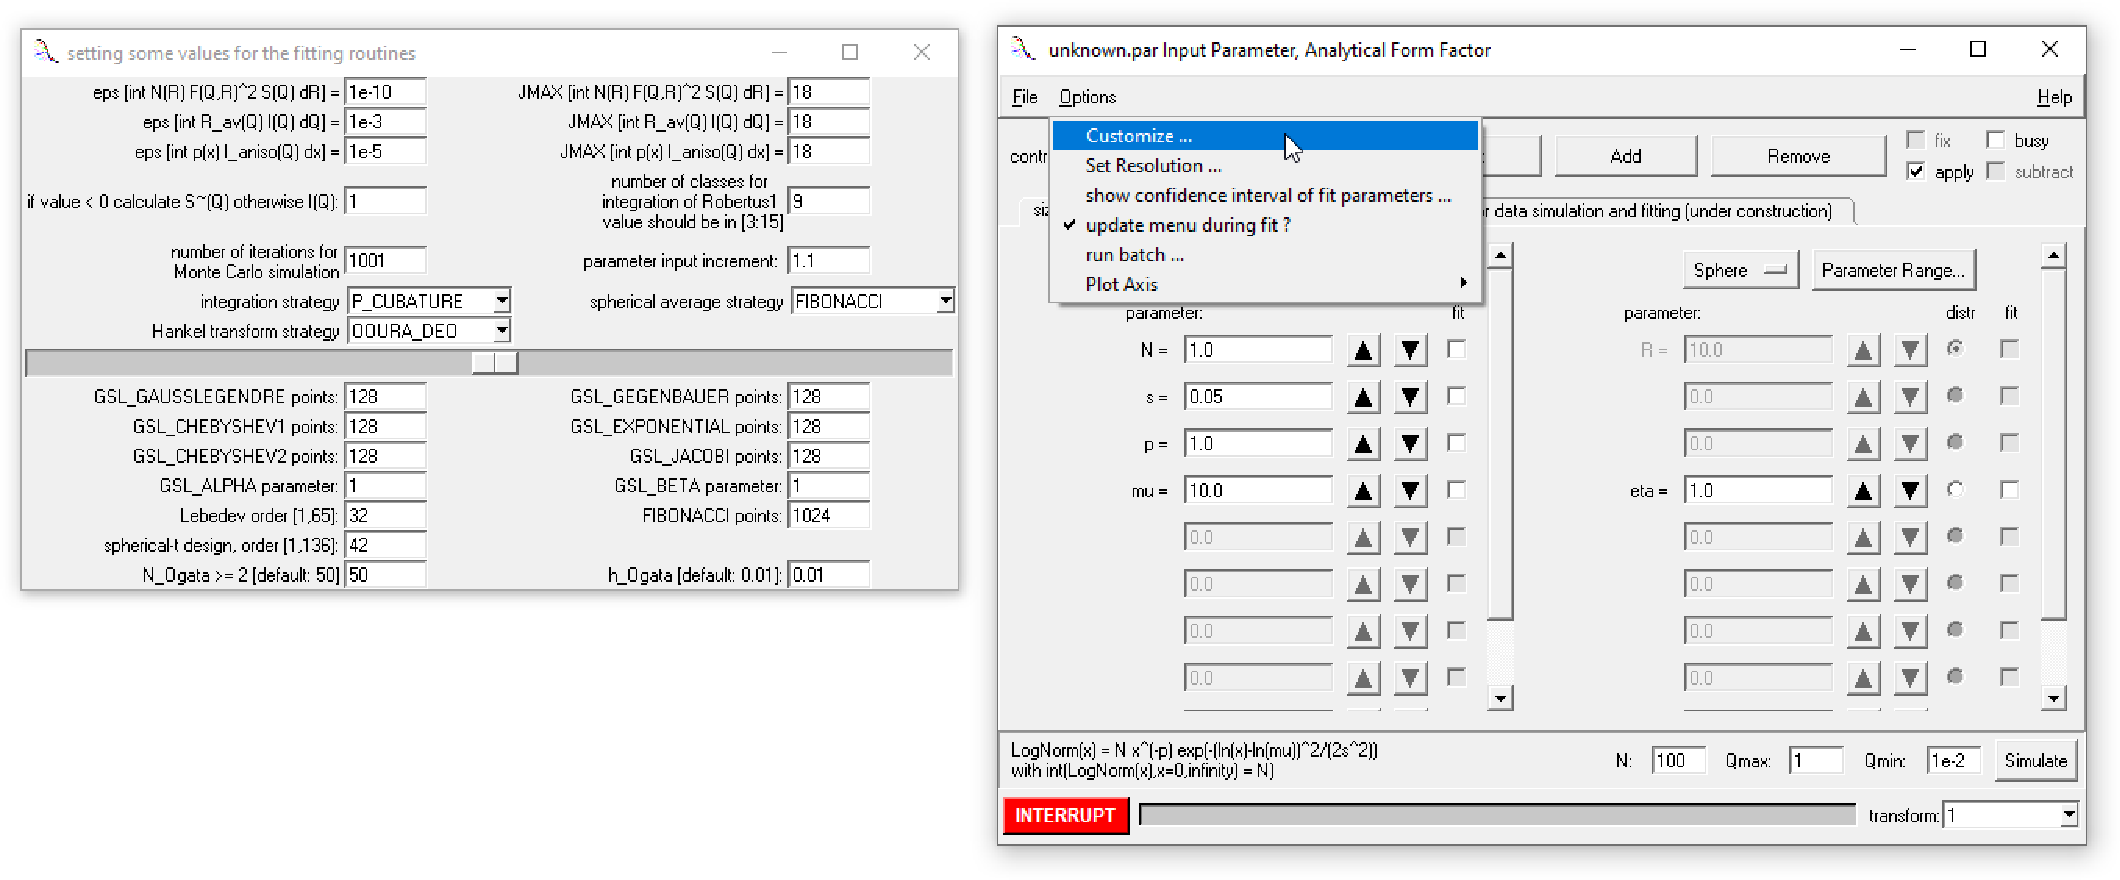
\includegraphics[width=0.95\textwidth]{../images/GUI/CustomizeWindow.pdf}
\end{center}
\caption{Menu for configuring internal integration routines in \SASfit}
\label{fig:CustomizeIntGUI}
\end{figure}

\subsection{Integration algorithms in SASfit for normal one- or multi-dimensional integration}  ~\\

Within \texttt{SASfit} a configurable one dimensional integration routine as well as a multidimensional one  with a common interface for the different algorithms is supplied. Depending on the mathematical behaviour of the integrant it has turned out that the different algorithms might differ a lot in terms of efficiency. For multidimensional quadrature algorithm so far the same strategy is used for all dimensions. The routines \texttt{sasfit\_integrate()}  and \texttt{sasfit\_cubature()} have the same configuration options. For multidimensional integrations either by itself specialized multidimensional algorithms or nested calls of one-dimensional integration routines are used. \\

\noindent Possible options for them are:\\
\begin{description}[font=\sffamily\bfseries, leftmargin=2.5cm,style=nextline,
                  nosep]
   \item[\texttt{OOURA\_DE}] double-exponential quadrature algorithm from \cite{Mori1990,Mori2001}
   \item[\texttt{OOURA\_CC}] Clenshaw-Curtis-quadrature using Chebyshev series expansion (\url{https://www.kurims.kyoto-u.ac.jp/~ooura/intcc.html})
   \item[\texttt{TANHSINH\_1}] TanhSinh quadrature \cite{Engelen2021,Engelen}
   \item[\texttt{TANHSINH\_2}] TanhSinh quadrature \cite{Engelen2021,Engelena}
   \item[\texttt{GSL\_QUAD}] quad integration routine from gsl \cite{Galassi2021}
   \item[\texttt{GSL\_QAG}] QAQ integration routine from gsl \cite{Galassi2021}
   \item[\texttt{GSL\_QNQ}] QNQ integration routine from gsl \cite{Galassi2021}
   \item[\texttt{H\_CUBATURE}] multidimensional integration routine \texttt{hcubature} from \cite{Johnson2017}
   \item[\texttt{P\_CUBATURE}] multidimensional integration routine \texttt{pcubature} from \cite{Johnson2017}
   \item[\texttt{GSL\_LEGENDRE}] Gauss-Legendre quadrature using gsl library  \cite{Galassi2021}
   \item[\texttt{MC\_MISER}] Monte-Carlo integration algorithm Miser using gsl library  \cite{Galassi2021}
   \item[\texttt{MC\_VEGAS}]  Monte-Carlo integration algorithm Vegas using gsl library  \cite{Galassi2021}
   \item[\texttt{MC\_PLAIN}]  plain Monte-Carlo integration algorithm using gsl library  \cite{Galassi2021}
   \item[\texttt{QMC\_HOLTON}] quasi Monte Carlo integration \cite{Zaslavsky2023} using the \texttt{gsl\_qrng\_halton} quasi random number generator from gsl \cite{Galassi2021}.
   \item[\texttt{QMC\_REVERSEHALTON}] quasi Monte Carlo integration \cite{Zaslavsky2023} using the \texttt{gsl\_qrng\_reversehalton} quasi random number generator from gsl \cite{Galassi2021}.
   \item[\texttt{QMC\_SOBOL}] quasi Monte Carlo integration \cite{Zaslavsky2023} using the \texttt{gsl\_qrng\_sobol} quasi random number generator from gsl \cite{Galassi2021}.
   \item[\texttt{QMC\_NIEDERREITER\_2}] quasi Monte Carlo integration \cite{Zaslavsky2023} using the reverse \texttt{gsl\_qrng\_niederreiter\_2} quasi random number generator from gsl \cite{Galassi2021}.
   \item[\texttt{RQMC\_SOBOL\_RDS}] randomized quasi Monte Carlo integration using the quasi random Sobol sequence with additional random digit scrambling \cite{Burley2020Scrambling}
   \item[\texttt{RQMC\_SOBOL\_OWEN}] randomized quasi Monte Carlo integration using the quasi random using Owen-scrambled Sobol sequence \cite{Burley2020Scrambling,Owen1995}
   \item[\texttt{RQMC\_FAURE05}] randomized quasi Monte Carlo integration using Owen-scrambled Faure (0,5) sequence \cite{Burley2020Scrambling,Owen1995}.
   \item[\texttt{RQMC\_LAINE\_KARRAS}] randomized quasi Monte Carlo integration using Laine-Karras hash method mentioned in \cite{Burley2020Scrambling} and given as C source code in its supplement information.
\end{description}

\section{orientation average} ~\\

Orientational averaging is a two dimensional integration over a unit sphere (\texttt{sasfit\_orient\_avg()}). In \texttt{SASfit} a specialized function for this is supplied. As the problem in principle can be handles with \texttt{sasfit\_cubature} it include all strategies from that function plus a few specialized one especially efficient for quadrature over a the surface of unit sphere. These are
\begin{description}
\item[\texttt{Lebedev}] Lebedev quadrature \cite{WikiLebedevQuad2024,Lebedev1975,Lebedev1976,Lebedev1977,Lebedev2003} is an approximation to the surface integral of a function over a three-dimensional sphere. The number and location of the grid points together with a corresponding set of integration weights are determined by enforcing the exact integration of polynomials (or equivalently, spherical harmonics) up to a given order.
\item[\texttt{FIBONACCI}]  Almost equally spaced points can be easily generated by a Fibonacci on different surfaces, like square, disk, cylinder surface, spherical surface \cite{Marques_2013,Swinbank2006}.
\item[\texttt{spherical\_t\_design}] The spherical t-design \cite{WikipediaSphericalDesign2024,Graef2011,Hardin1996} has been used to generate equally spaced points on a spherical surface leading to a quadrature formula with equal weights.
\end{description}

\subsection{Hankel transform} ~\\

The Hankel transform calculated by \texttt{sasfit\_hankel()} is defined by
\begin{align}\label{eq:HT}
F(q) &= \mathcal{H}_n\left[f(q)\right](r)  = \int_0^\infty \mathrm{J}_n(qr) f(r) r \mathrm{d}r
\end{align}
This means an upper unbounded integral over the oscillating Bessel function $\mathrm{J}_n()$ has to be solved numerically.
Thos strategies already available for functions with an strictly periodic $\cos()$ or $\sin()$ term (Fourier type) can not be directly been used as only for large arguments of the bessel function in behaves as $\mathrm{J}_n(x)\approx \sqrt{\frac{2}{\pi x}}\cos\left(x-\frac{\pi}{2}n-\frac{\pi}{4}\right)$.
\begin{description}
\item[\texttt{QWE}] Quadrature With Extrapolation computes an
infinite integral using the partial sum of quadrature terms
accelerated by sequence extrapolation using the Shanks transformation
implemented with Wynn's epsilon algorithm \cite{Key2012}.
\item[\texttt{CHAVE}]  This algorithm performs the integration of the product of the kernel and Bessel functions between the asymptotic zero crossings of the latter and sums the series of partial integrations using a continued fraction expansion, equivalent to an analytic continuation of the series \cite{Chave1983}.
\item[\texttt{OOURA\_DEO}] As for large arguments $x$ the Bessel function asymptotically behaves as
$\mathrm{J}_n\approx \sqrt{\frac{2}{\pi x}}\cos\left(x-\frac{\pi}{2}n-\frac{\pi}{4}\right)$ the double exponential formula of \cite{Ooura_1991} for oscillatory functions over the half infinite interval is used directly.
\item[\texttt{GSL\_QAWF}] This options tries to make use of the adaptive integration of Fourier integrals available in the gsl library (\texttt{gsl\_integration\_qawf()}). This function attempts to compute a Fourier integral of the function $g$ over the semi-infinite interval $[a,+\infty)$ as
$I = \int_a^{+\infty} \mathrm{d}x g(x)
\left\{
\begin{array}{c}
\sin{(\omega x)} \\
\cos{(\omega x)}
\end{array}
\right\}$
By defining $g(r)= f(r) \frac{\mathrm{J}_n(qr)}{\cos\left(qr-\frac{\pi}{2}n-\frac{\pi}{4}\right)}$ we convert the Hankel transform in \ref{eq:HT} into a $\cos$-Fourier type transform after an additional substitutions of $r'=r-\frac{\pi}{2}\frac{n}{q}-\frac{1}{q}\frac{\pi}{4}$.
\end{description}
Next to the quadrature algorithms above also fast digital filters for Hankel transform have been developed. A few of these have been supplied in SASfit for testing \cite{Anderson1989,Guptasarma1997,Ogata2005,Kong2007,Key2012,Kang2021}: \\
\texttt{OGATA\_2005}, \texttt{FBT0}, \texttt{FBT1}, \texttt{FBT2}, \texttt{GUPTASARMA\_97}, \texttt{GUPTASARMA\_97\_FAST}, \texttt{KEY\_51}, \texttt{KEY\_101}, \texttt{KEY\_201}, \texttt{ANDERSON\_801}



\clearpage
\section{Fitting strategies}

\clearpage
\section{Data I/O Formats}

\subsection{Input Format} \hspace{1pt}\\

\SASfit supports a simple ASCII format. Options for reading ASCII
data can be set in the corresponding menu, where one can set an
input format and the number of lines to be skipped at the beginning
of the data file. To set an input format one has to supply a string
like "{\tt xyer}". Each line which does not contain valid float
numbers are skipped automatically. Each line further should at least
contain as many valid numbers as the supplied format string
characters. That means if the line contains only three numbers but
the format string is 4 or more characters long the line will be
ignored. Separators between numbers can be "white space",
"tabulator", or ",". For identifying the columns the characters and
their position in the string are interpreted. {\tt x}, {\tt y} and
{\tt e} stands for the scattering vector $Q$, scattering intensity
$I(Q)$ and its error $\Delta I(Q)$, respectively. {\tt r} defines
the column for a resolution parameter $\sigma$. The position of the
character in the string defines which data column is assigned to
$Q$, $I(Q)$, $\Delta I(Q)$, and $\sigma$. In case of double
occurrence of a character the position of the last one is the
significant position. Any characters not belonging to \{{\tt x},{\tt
y},{\tt e},{\tt r}\} can be used to skip a column. A definition
string need to contain
at least the two characters {\tt x} and {\tt y}. \\

\begin{description}
\item[Example 1 (BerSANS format)] ~\\
{\tiny
\begin{verbatim}
%File
FileName=D0002831.200 FileDate=28-Jun-99 FileTime=11:57:16
Type=SANSDIso Title=IMF
%Counts
 2.651E-02, 2.372E+02, 4.650E+00
 3.240E-02, 2.170E+02, 2.291E+00
 3.829E-02, 1.898E+02, 1.713E+00
 4.418E-02, 1.743E+02, 1.479E+00
 5.007E-02, 1.528E+02, 1.318E+00
 5.596E-02, 1.361E+02, 1.153E+00
\end{verbatim}
} \centerline{$\vdots$ \hspace{5cm} ~}
~\\
As the first lines start with a string, they will be automatically
ignored. To interpret the three columns as $Q$, $I(Q)$, $\Delta
I(Q)$ the format string should be simply {\tt xyz}. The BerSANS
format can also be read in by explicitly selecting  
the "BerSANS"-format button in the menu instead of the
"ASCII"-format. \\[1cm]

\item[Example 2] \hspace{1pt}\\
{\tiny
\textcolor[rgb]{0.98,0.00,0.00}{$\mathbf{\lceil}$}
\verb"      19         0         0         0         0         0         0         6"\\
\verb"  0.100000E+01   0.100000E+04   0.000000E+00   0.100000E+01   0.120000E+01"\\
\verb"  0.000000E+00   0.000000E+00   0.000000E+00   0.000000E+00   0.000000E+00"
\textcolor[rgb]{0.98,0.00,0.00}{$\mathbf{\rfloor}$}
\begin{verbatim}
teflon              instrument tests
1  2.617993E-04   3.700000E+01   4.301163E+00
2  1.062462E-03   6.412500E+01   1.634587E+00
3  2.107973E-03   1.410135E+03   5.207492E+00
4  3.167636E-03   1.752197E+03   4.801586E+00
5  4.189463E-03   7.581771E+02   2.810281E+00
                   :
                   :
45  1.255376E-02   1.486688E+01   2.197023E-01
46  1.360724E-02   1.204012E+01   1.927716E-01
47  1.466810E-02   1.026648E+01   1.679423E-01
\end{verbatim}
}
~\\
A definition string {\tt ixye} would ignore the leading line number
at the beginning of each data line, but in the present example also
the first 3 lines would also be interpreted as data points. To skip
them one has to use the option for skipping leading lines in a data
file. In the above case the number should be set to 3 or 4. As the
4$^\text{th}$ line is anyway ignore a value of 3 is sufficient to
skip non data points.
\\[1cm]

\item[Example 3] ILL data files from regrouped treatment ({\tt gnnnnnn.eee}).\\
{\tiny
\begin{verbatim}
 Sample - d corrs    TEST prot/deutr. ellipt. chs  44 lines+(Q, I(Q), errI(Q))
  ILL  SANS D11
\end{verbatim}
\textcolor[rgb]{0.98,0.00,0.00}{$\mathbf{\lceil}$}
\verb"        8303         1        37         1        42        38"\\
\textcolor[rgb]{1.0,1.00,1.00}{$\mathbf{\lceil}$}
\verb"           14        32         0         3         1"
\textcolor[rgb]{0.98,0.00,0.00}{$\mathbf{\rfloor}$}
\begin{verbatim}
  spol 20-Oct-1995  9:16:09
   AvA1 0.0000E+00 AsA2 9.5000E-01 XvA3 1.0000E+00 XsA4 1.0000E+00 XfA5 0.0000E+00
  S...  8303  0  1.00E+00 P100 0.5% 221   Sbak  8309  0  2.00E+00 Blank523 193
  V...  8301  0  1.00E+00 Hhaps 911

    0.0000 ! Theta-0 Detector offset angle
   32.5000 ! X0 cms Beam centre
   32.5000 ! Y0 cms Beam centre
    1.0000 ! Delta-R cms regrouping step
    2.5000 ! SD m Sample-detector distance
   10.5400 ! Angstroms incident wavelength
    5.6000 ! m collimation distance
    1.0000 ! concentration
       -3. ! ISUM central window sum
        1. ! flux monitor counts
  180.0000 ! degrees detector sector width
    0.0000 ! degrees sector orientation
   10.0000 ! % wavelength spread
   20.0000 ! mm source slit width x
    0.0000 ! mm source slit height y
   10.0000 ! mm sample width x
    0.0000 ! mm sample height y
   10.0000 ! mm detector x pixel size
   10.0000 ! mm detector y pixel size
    0.0000 ! degrees sample normal/beam
    0.0000 ! K sample temperature
    0.0000 ! sample transmission
    1.0000 ! mm sample thickness
  900.0000 ! secs counting time
    0.0000 ! reserved
    0.0000 ! reserved
    0.0000 ! reserved
    0.0000 ! reserved
    0.0000 ! reserved
    0.0000 ! reserved
    0.0000 ! reserved
    0.0000 ! reserved
\end{verbatim}
\textcolor[rgb]{0.98,0.00,0.00}{$\mathbf{\lceil}$}
\verb"         37         0         0         0         0         0         0         6"\\
\textcolor[rgb]{1.0,1.00,1.00}{$\mathbf{\lceil}$}
\verb"    0.100000E+01   0.250000E+03   0.000000E+00   0.100000E+01   0.105400E+01"\\
\textcolor[rgb]{1.0,1.00,1.00}{$\mathbf{\lceil}$}
\verb"    0.000000E+00   0.000000E+00   0.000000E+00   0.000000E+00   0.000000E+00"\\
\textcolor[rgb]{1.0,1.00,1.00}{$\mathbf{\lceil}$}
\verb"0.000000E+00   0.000000E+00   0.000000E+00"
\textcolor[rgb]{0.98,0.00,0.00}{$\mathbf{\rfloor}$}
\begin{verbatim}
    2.194656E-03   3.442688E-01   8.329221E-02
    5.466116E-03   3.000000E-01   5.008947E-02
    8.480323E-03   3.877941E-01   4.232426E-02
    1.189216E-02   6.498784E-01   1.519078E-02
    1.497785E-02   7.493181E-01   1.173622E-02
\end{verbatim}
\centerline{$\vdots$ \hspace{5cm} ~} }
\noindent To read in a
regrouped ILL data file one has to use the definition string {\tt
xye} and secondly one has to skip the first 44 lines in the data
file to ignore also the lines marked with
\textcolor[rgb]{0.98,0.00,0.00}{$\mathbf{\lceil}$}
\textcolor[rgb]{0.98,0.00,0.00}{$\mathbf{\rfloor}$}. If one does not
skip the first 44 lines the marked lines are interpreted erroneously
also as data points. The other lines at the beginning of the data
file are ignored as they do not fulfill the condition that they have
3 columns containing only valid numbers.
\end{description}

\subsection{Error bar} \hspace{1pt}\\

\noindent
In case no error bar is supplied \SASfit will try to guess one.
To do this an polynomial $y_p(Q)$ of degree $p$
\begin{align}
y_p(Q) &= \sum_{k=0}^p c_k Q^k
\end{align}
is fitted to the data point $i$ and its $n^\textrm{th}$ neighbors to the left and right,
i.e. is fitted to $2n+1$ points from $I_{i-n}(Q_{i-n})$ to $I_{i+n}(Q_{i+n})$.
After the fit $\chi_i^2$ is calculated
\begin{align}
\chi_i^2&=\sum_{j=i-n}^{i+n} \left(I_j(Q_j)-y_P(Q_j)\right)^2
\end{align}
The error bar $\Delta I_i$ for $Q_i$ is than defined as
\begin{align}
\Delta I_i &= \sqrt{\frac{\chi_i^2}{2n-p}}
\end{align}
\SASfit is using two nearest neighbors $n=2$ and fitting a polynomial of \
degree $p=2$ to it to guess an error bar.
This procedure gives reasonable error bars as long as the data are oversampled and do not show sharp features within the data points $i-n$ and $i+n$. A diffraction peak or a minimum in a form factor like for monodisperse particle might not reasonable well described by the polynomial and consequently the resulting error bar will get large. Furthermore systematic errors in the absolute intensity like an overall scaling factor will not be recognized. The procedure to guess the error bar is basing on the assumption that the scattering curve behaves locally approximately like a polynomial function of degree $p=2$.

\begin{figure}[htb]
\begin{center}
\subfigure[simulated model data set with supplied error bars]{\label{fig:ModelDataWithError}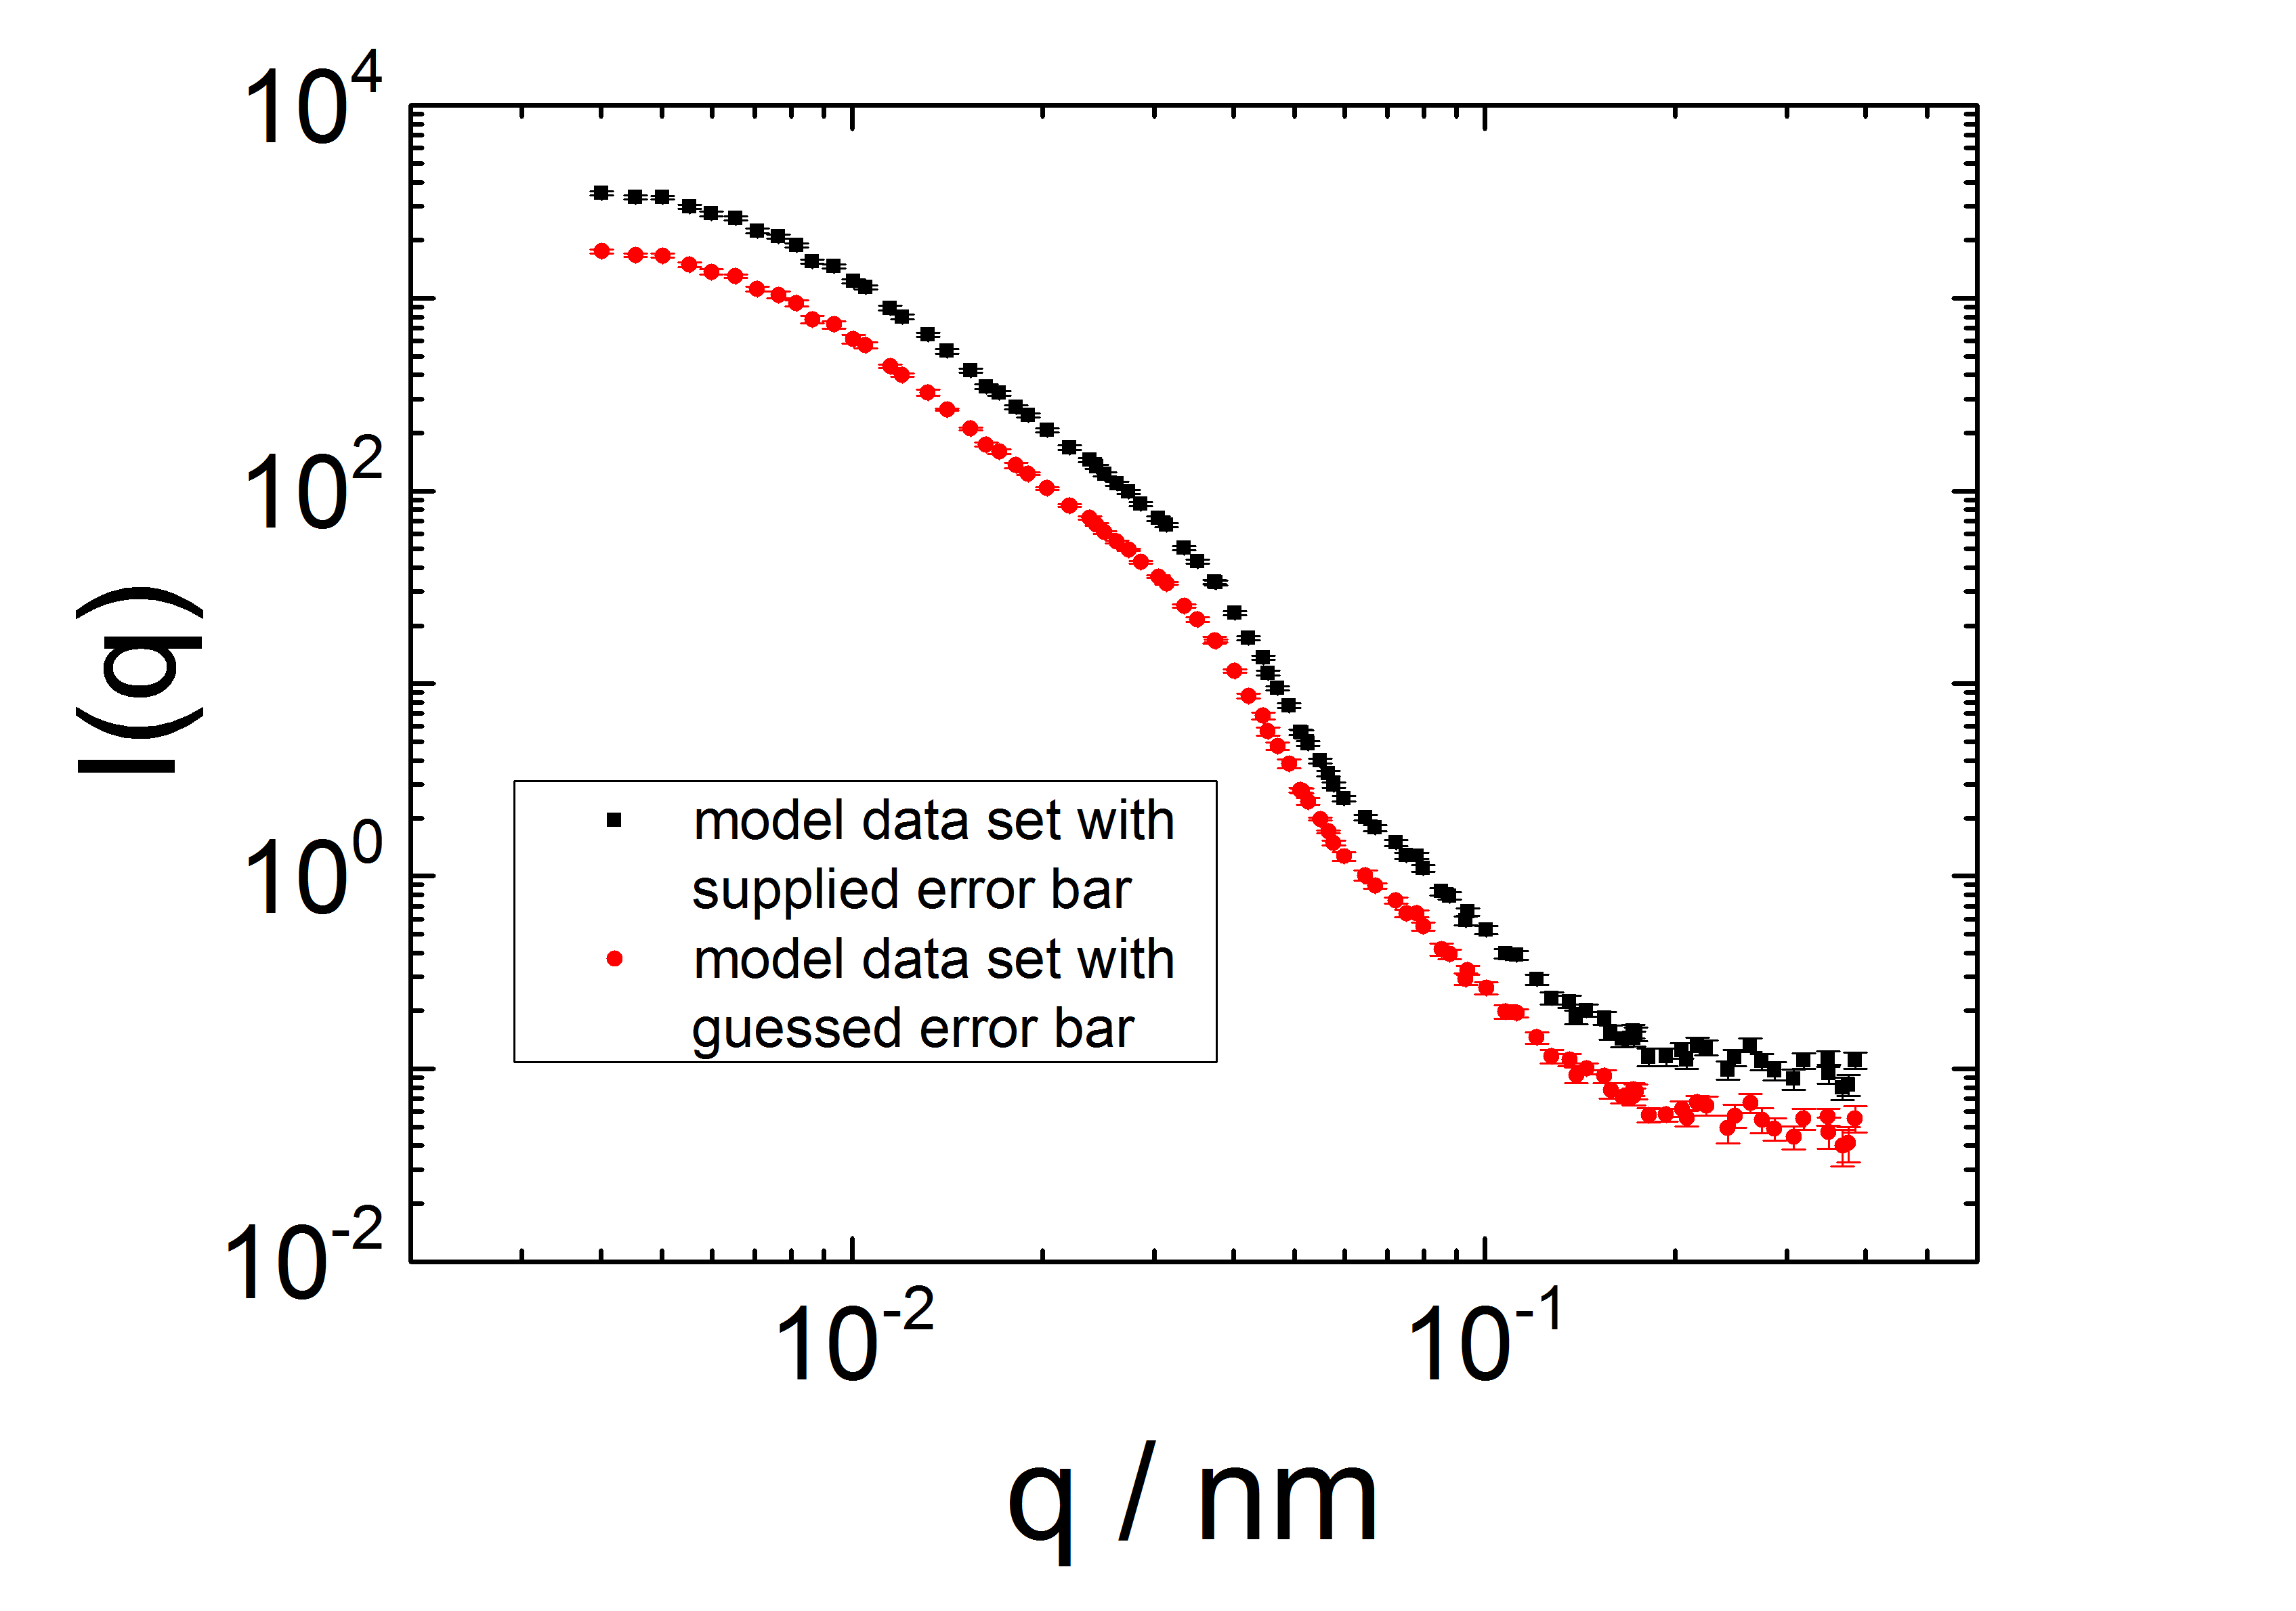
\includegraphics[width=0.47\textwidth]{../images/ErrorBar/ModelDataWithError.png}}
\subfigure[Ratio between supplied error bar and the error bar guessed by \SASfit]{\label{fig:ErrorGUI}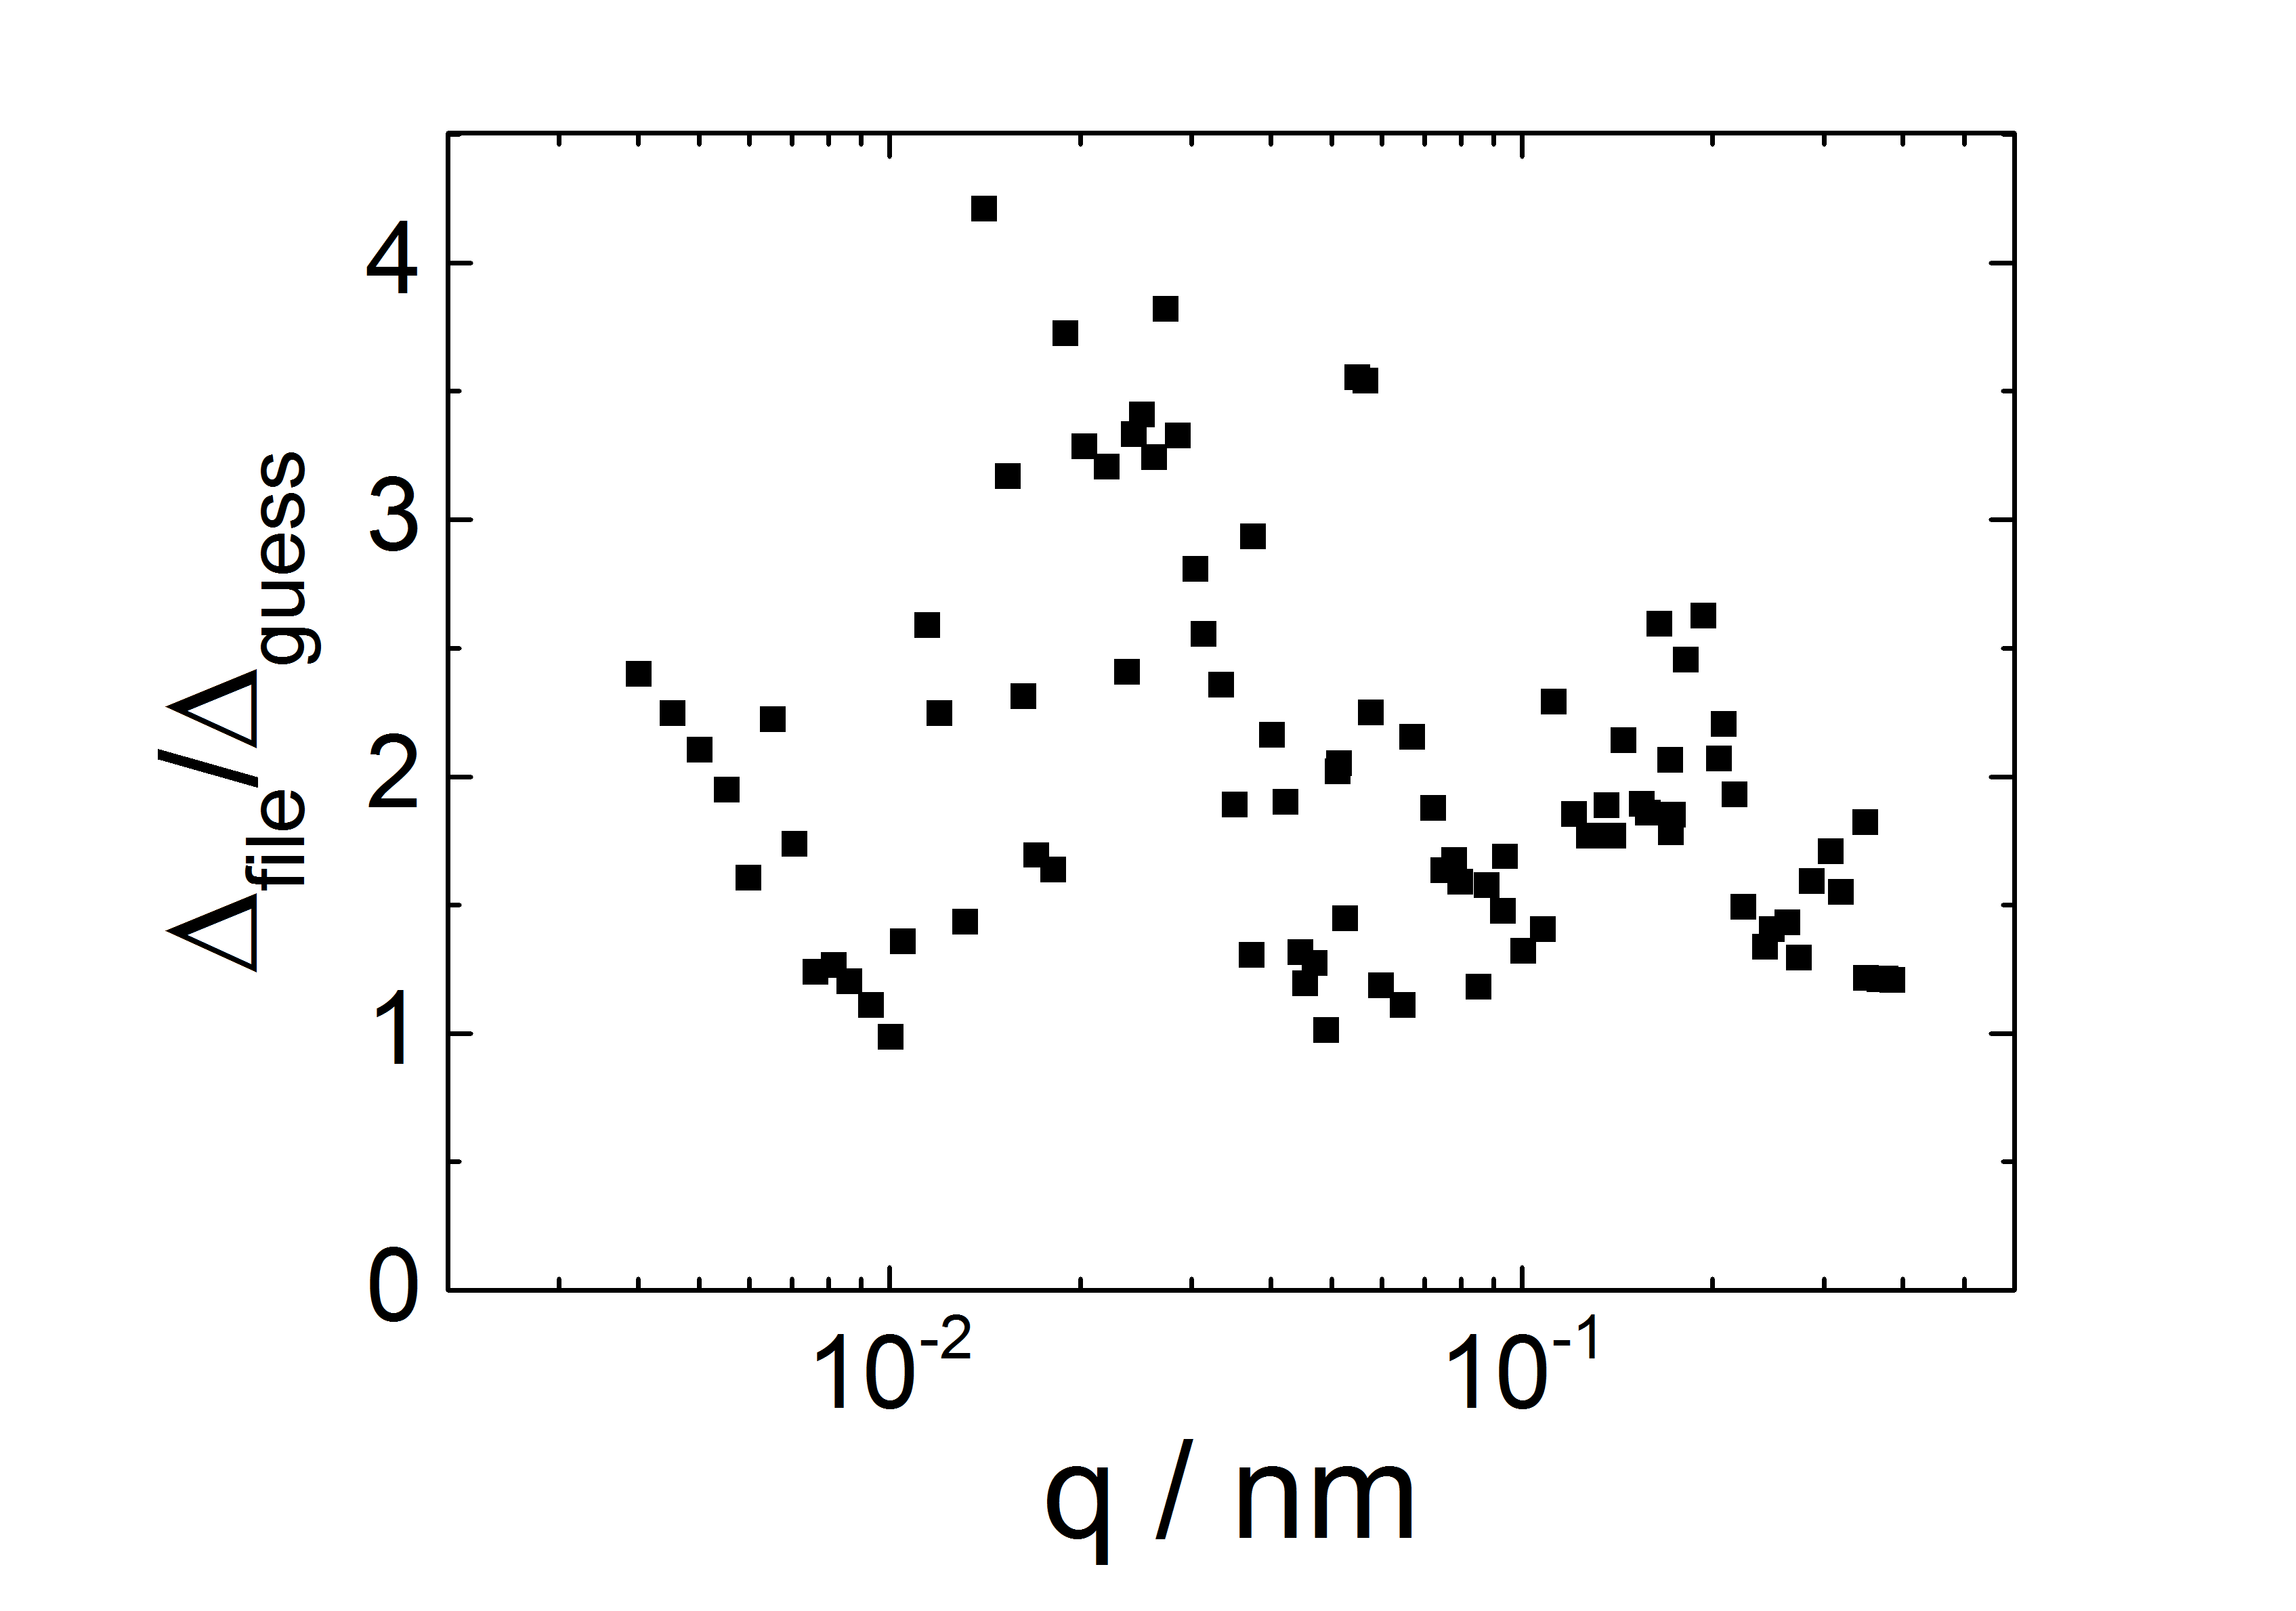
\includegraphics[width=0.47\textwidth]{../images/ErrorBar/RatioErrSuppGuess.png}}
\end{center}
\caption{Comparison of a simulated model data set with supplied error bar and an error bar guessed by \SASfit.}
\label{fig:ErrBar}
\end{figure}

\vspace{1cm}

\subsection{Export Format} \hspace{1pt}\\

\noindent
{\bf Example for an exported data file:}\\
{\tiny
\begin{verbatim}
  0.00401571,      3497.47,      90.7282,            0,   0.00401571,       260294,           -1,            0,
  0.00454087,         3340,      84.9531,            0,   0.00454087,       254548,           -1,            0,
   0.0050096,      3322.47,      79.6313,            0,    0.0050096,       248833,           -1,            0,
  0.00552335,      2983.23,      73.7254,            0,   0.00552335,       241949,           -1,            0,
  0.00598495,      2737.17,      68.4395,            0,   0.00598495,       235226,           -1,            0,
   0.0065309,      2598.76,      62.3109,            0,    0.0065309,       226647,           -1,            0,
  0.00706977,       2233.9,      56.4829,            0,   0.00706977,       217551,           -1,            0,
  0.00764207,      2080.96,      50.6186,            0,   0.00764207,       207264,           -1,            0,
  0.00815988,      1882.88,      45.6557,            0,   0.00815988,       197459,           -1,            0,
\end{verbatim}
\centerline{$\vdots$ \hspace{5cm} $\vdots$}
\begin{verbatim}
            ,             ,             ,             ,    0.0445634,      1535.14,           -1,            0,
            ,             ,             ,             ,    0.0453557,      1473.71,           -1,            0,
            ,             ,             ,             ,    0.0470219,      1340.34,           -1,            0,
            ,             ,             ,             ,    0.0490017,      1192.64,           -1,            0,
            ,             ,             ,             ,    0.0510837,      1055.44,           -1,            0,
\end{verbatim}
} If one like to export the data of an $xy$-plot all curves are
stored in a single data file. Each curve will occupy four columns
($Q$, $I(Q)$, $\Delta I(Q)$, $\sigma$). If an error $\Delta I(Q)$ is
not available, e.g. for theoretical data curves, the corresponding
column will be filled with -1. Similar is valid for the resolution
parameter $\sigma$ which will be set to 0 in case it is not
available. The individual columns are separated by ",". If the curve
have different amount of data points the column will be filled with
empty space for the missing data. This comma separated data format
has been chosen as it can be imported easily by many commercial
plotting softwares. The drawback of this format is, however, that
\SASfit cannot read it correctly, if the individual curves are of
different length.

\clearpage
\section{Scattering length density calculator}
\label{sec:SLDcalculator}

The \texttt{SLD calculator} is using thermal neutron cross-sections
only to calculate neutron scattering length density. For x-rays the
energy dependent scattering coefficients $f'$ and $f''$ are derived
using the theoretical approximation developed by Cromer and
Liberman. This theory gives accurate values far from an absorption
edge but does not account for the effects of neighboring atoms,
which can be very substantial near an absorption edge. Before
conducting an anomalous scattering experiment close to an absorption
edge it is therefore advisable to determine the actual scattering
behavior of the sample. The x-ray data have been taken from
\url{http://skuld.bmsc.washington.edu/scatter/AS_periodic.html} and
those for neutrons from
\url{http://www.ncnr.nist.gov/resources/n-lengths/list.html}.
\begin{figure}[htb]
\begin{center}
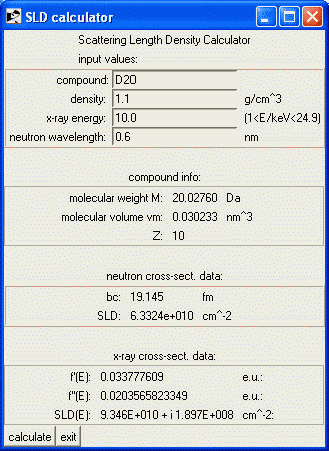
\includegraphics[width=0.329\textwidth,height=0.451\textwidth]{SLDcalculator.png}
\end{center}
\caption{Input menu for the scattering length density calculator}
\label{fig:SLDcalculator}
\end{figure}
The menu interface in Fig.\ \ref{fig:SLDcalculator} has for input
parameters, the sum formulae of the compound, its mass density in
g/cm$^3$, the x-ray energy in keV and the neutron wave length in nm.
In the compound name non-integer stoichiometry is supported, e.g.
H0.2O0.1 and H2O will calculate the same scattering length density.
However, the molecular volume $v_m$ and the molecular weight $M$ of
cause depend on such differences. The elements in the compound name
are case sensitive. Therefore you have to use \texttt{SiO2} instead
of \texttt{SIO2}. Also isotopes are handled like \texttt{C(13)}
(Carbon-13), \texttt{H(2)} (Deuterium), or \texttt{O(18)}
(Oxygen-18). For Deuterium next to \texttt{H(2)} also \texttt{D} can
be used.

Examples of how to format the compound name:
\begin{itemize}
\item Magnetite: \texttt{Fe3O4}, 5.15 g/cm$^3$
\item Eucryptite: \texttt{LiAlSiO4}, 2.67 g/cm$^3$
\item protonated toluene, \texttt{C7H8}, 0.865 g/cm$^3$
\item deuterated toluene, \texttt{C7D8} or \texttt{C7H(2)8}, 0.94 g/cm$^3$
\item mixture of 65/35 heavy water/light water, \texttt{(D2O)0.65(H2O)0.35}, 1.065 g/cm$^3$
\end{itemize}
From the compound name and the density first the molecular weight $M$, molecular volume $v_m$,
and total number of electrons $Z$ are calculated. Together with the tabulated neutron scattering length and
tabulated energy dependent scattering coefficient $f'(E)$ and $f''(E)$ the corresponding coherent
neutron scattering length $b_c=\sum_i b_i$, coherent neutron scattering length density
$\eta_{n,SLD}=b_c/v_m$  and
for x-rays the complex energy dependent scattering scattering length density
$\eta_{x,SLD}=\left(Z-(Z/82.5)^{2.37}+f'(E)+\imath f''(E)\right)/v_m$ of the compound are calculated.

\clearpage
\clearpage
\section{Resolution Function \cite{Pedersen1990}}
%\begin{subequations}
\begin{align}
    \langle k\rangle      & = 2 \pi/\lambda \\
    \langle \theta\rangle  &= \arcsin(\langle Q_{av}/(2 \langle k\rangle )) \\
    a_1        &= \frac{r_1}{L+l/\cos^2(2\langle \theta\rangle )} \\
    a_2        &= r_2 \cos^2(2 \langle \theta\rangle )/l \\
    \Delta\beta_1 &=
       \begin{cases}
          a_1 \geq a_2: & \displaystyle \frac{2 r_1}{L} - \frac{r_2^2}{2 r_1}
          \frac{\cos^4(2\langle \theta\rangle )}{l^2L}
                          \left(L+\frac{l}{\cos^2(2\langle \theta\rangle )}\right)^2\\
                          ~
                          \\
          a_1 < a_2: & \displaystyle 2 r_2\left(\frac{1}{L} + \frac{\cos^2(2\langle \theta\rangle )}{l}\right)
                 - \frac{r_1^2}{2r_2}  \frac{l}{L} \\
                 & \displaystyle \times
                 \frac{1}{\cos^2(2\langle \theta\rangle ) \left(L+\frac{l}{\cos^2(2\langle \theta\rangle )}\right)}
       \end{cases}
\end{align}
%\end{subequations}
%\begin{subequations}
\begin{align}
    \sigma_W  &= \langle Q\rangle \frac{\Delta\lambda}{\lambda}\frac{1}{2\sqrt{2\ln(2)}} \\
    \sigma_{C1} &= \langle k\rangle\cos(\langle \theta\rangle)\frac{\Delta\beta_1}{2\sqrt{2\ln(2)}}  \\
    \sigma_{D1} &= \langle k\rangle\cos(\langle \theta\rangle)\cos^2(2\langle \theta\rangle) \frac{D}{l \,2\sqrt{2\ln(2)}} \\
    \sigma_{av} &= \langle k\rangle\cos(\langle \theta\rangle)\cos^2(2\langle \theta\rangle) \frac{\Delta D}{l \,2\sqrt{2\ln(2)}} \\
    \sigma &= \sqrt{\sigma^2_W+\sigma^2_{C1}+\sigma^2_{D1}+\sigma^2_{av}}
\end{align}
%\end{subequations}
\begin{equation}
R_{av}\left(Q,\langle Q\rangle\right) = \frac{Q}{\sigma^2}
 \exp\left( -\frac{1}{2}\left(Q^2+\langle Q\rangle^2\right)/\sigma^2\right)
 I_0(Q\langle Q\rangle/\sigma^2)
\end{equation}

\begin{equation}
I(\langle Q\rangle) = \int_0^\infty R_{av}\left(Q,\langle
Q\rangle\right) \frac{d\sigma}{d\Omega}(Q) \, dQ
\end{equation}
\begin{equation}
\frac{d\sigma}{d\Omega}(Q) = \int_0^\infty N(R) F^2(Q,R) \, dR
\end{equation}

\clearpage
%\chapter{Analytical Size Distribution, Form Factors, and Structure factors}
%\label{SDFFSQ}

\chapter{Form Factors}
\label{formfactor}

\section{Spheres \& Shells}
\label{sect:Spheres_Shells}

\subsection{Sphere}
\label{sect:sphere} ~\\

\begin{figure}[htb]
\begin{center}
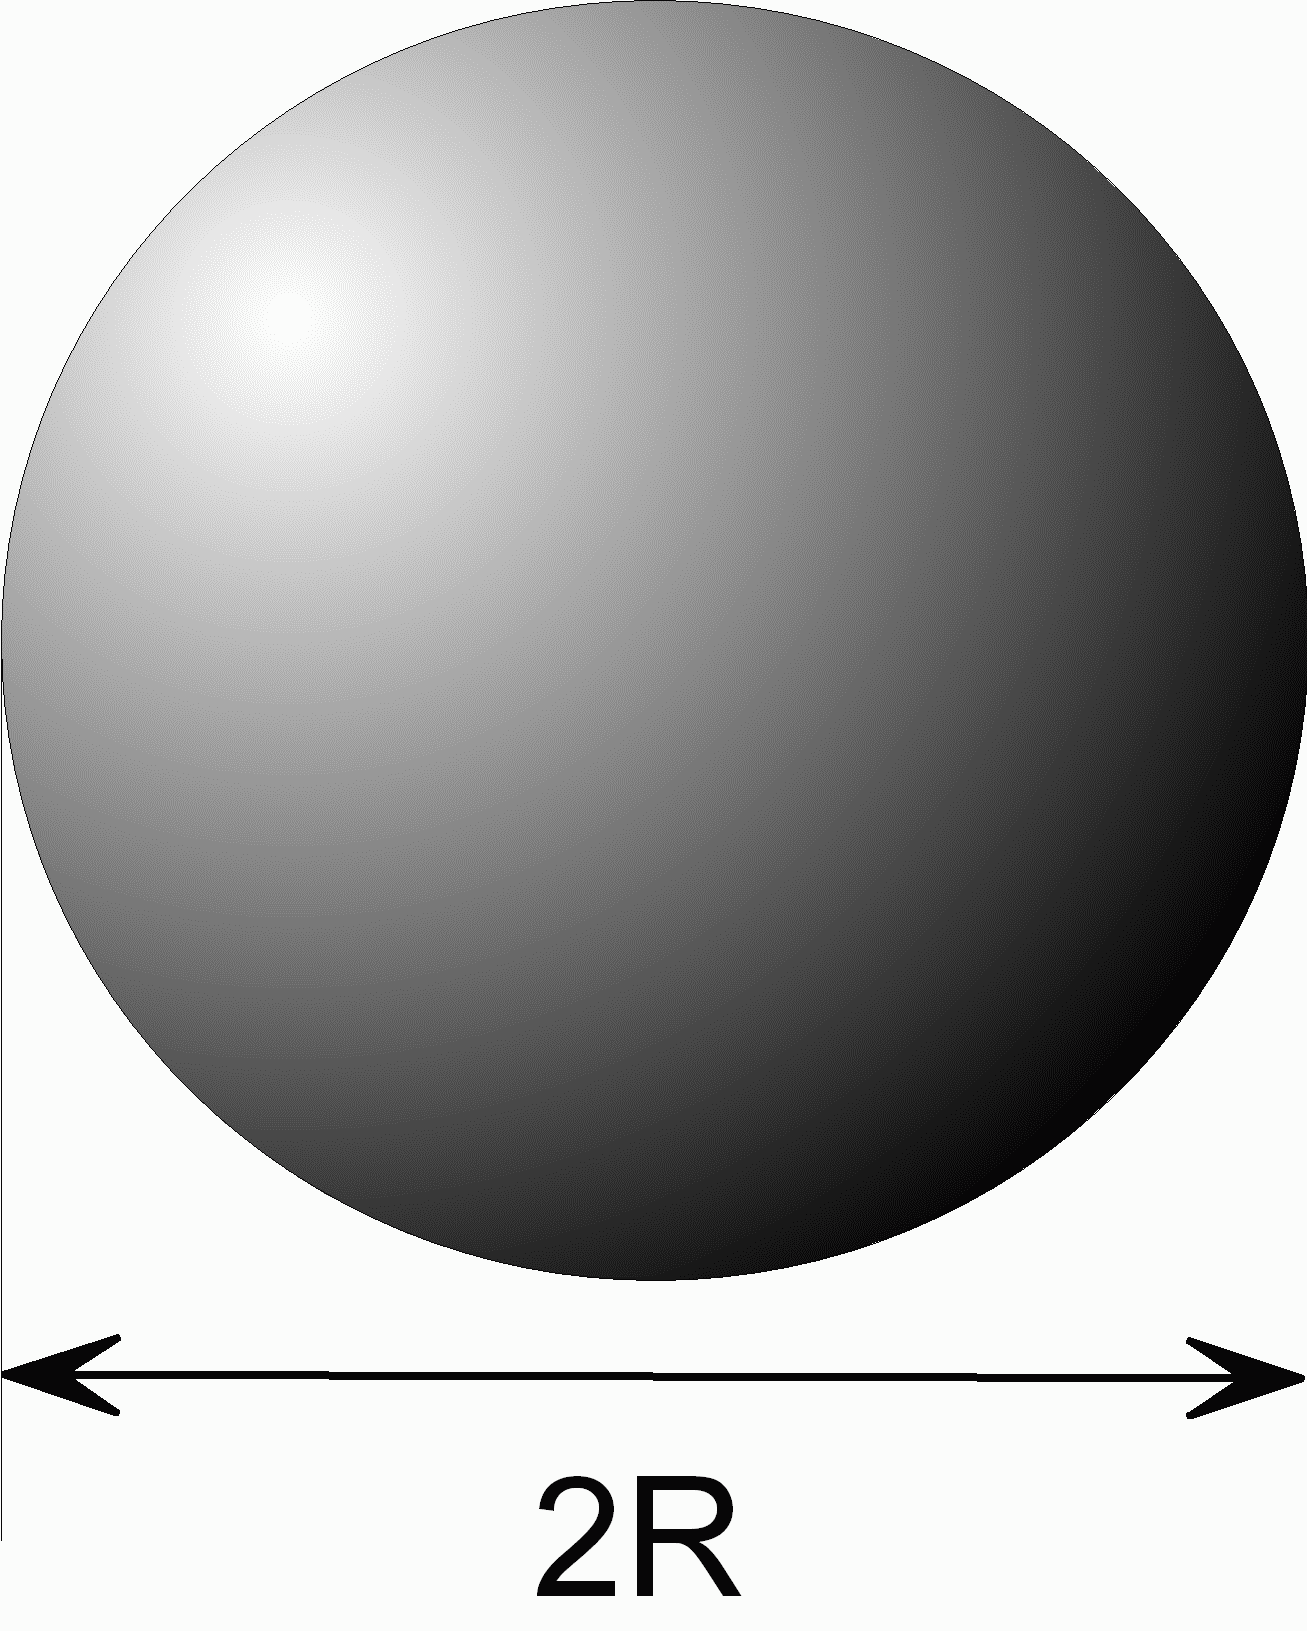
\includegraphics[width=0.2875\textwidth,height=0.359\textwidth]{../images/form_factor/spheres/sphere.png}
\end{center}
\caption{Sphere with diameter $2R$} \label{fig:Sketch_sphere}
\end{figure}

\begin{subequations}
\begin{align}
I_\text{Sphere}(Q,R) = K^2(Q,R,\Delta\eta) \label{eq:I_sphere}
\end{align}
with
\begin{align}
 K(Q,R,\Delta\eta) = \frac{4}{3}\pi R^3 \Delta\eta \, 3 \frac{\sin QR - QR \cos QR}{(QR)^3}
\end{align}
The forward scattering for $Q=0$ is given by
$$
\lim_{Q=0}I_\text{Sphere}(Q,R) =\left( \frac{4}{3}\pi R^3 \Delta\eta \right)^2
$$
\end{subequations}

\vspace{5mm}
\noindent \underline{Input Parameters for model \texttt{Sphere}:}
\begin{description}
\item[\texttt{R}] radius of sphere $R$
\item[- - -] not used
\item[- - -] not used
\item[\texttt{eta}] scattering length density difference between particle and matrix $\Delta\eta$
\end{description}

\noindent\underline{Note:}
\begin{itemize}
\item The parameters \texttt{param.p[1]} and \texttt{param.p[2]} are not used.
\end{itemize}

\begin{figure}[htb]
\begin{center}
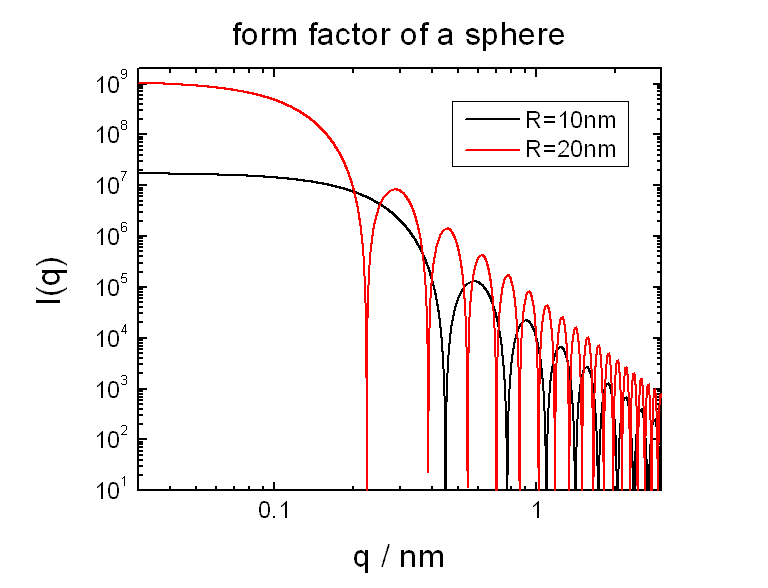
\includegraphics[width=0.768\textwidth,height=0.588\textwidth]{../images/form_factor/spheres/sphere_P.png}
\end{center}
\caption{Scattering intensity of spheres with radii $R=10$nm and $R=20$nm.
The scattering length density contrast is set to 1.} \label{fig:I_sphere}
\end{figure}

%%%%%%%%%%%%%%%%%%%%%%%%%%%%%%%%%%%%%%%%%%%%%%%%%%%%%%%%%%
\clearpage

\subsection{Spherical Shell i}
\label{sect:spherical_shell_i} ~\\

\begin{figure}[htb]
\begin{center}
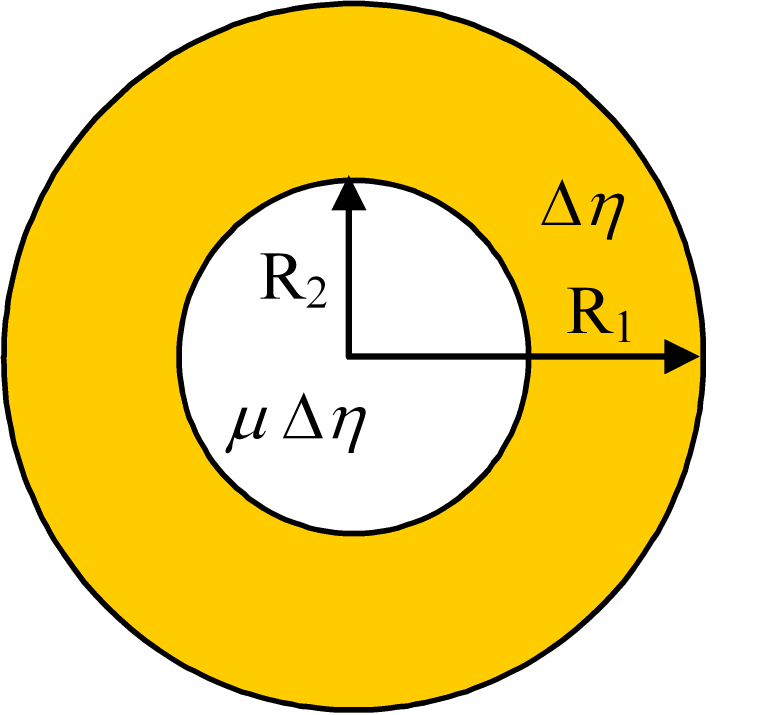
\includegraphics[width=0.38\textwidth,height=0.3575\textwidth]{../images/form_factor/spheres/shell1.png}
\end{center}
\caption{Spherical Shell i} \label{fig:shell1}
\end{figure}

This implementation of a spherical shell is parametrised with an inner radius $ R_2$ and outer
radius $R_1$. The scattering contrast relative to the matrix of the core is $\mu \Delta \eta$
and the one of the shell $\Delta\eta$.

\begin{align}
I_\text{Shell1}(Q,R_1,R_2,\Delta\eta,\mu)=
\left[K(Q,R_1,\Delta\eta)-K(Q,R_2,\Delta\eta(1-\mu))\right]^2
\end{align}
with
\begin{align}
 K(Q,R,\Delta\eta) = \frac{4}{3}\pi R^3 \Delta\eta \, 3 \frac{\sin QR - QR \cos QR}{(QR)^3}
\end{align}
The forward scattering for $Q=0$ is given by
$$
\lim_{Q=0}I_\text{Shell1}(Q,R_1,R_2,\Delta\eta,\mu) =
\left(\frac{4}{3}\pi \Delta\eta \left[ R_1^3 -
R_2^3(1-\mu)\right]\right)^2
$$

\vspace{5mm}
\noindent  \underline{Input Parameters for model \texttt{Spherical Shell i}:}
\begin{description}
\item[\texttt{R1}] overall radius of spherical shell $R_1$
\item[\texttt{R2}] radius of core $R_2$
\item[\texttt{eta}] scattering length density difference between shell and matrix $\Delta\eta$
\item[\texttt{mu}] scattering length density difference between core and matrix relative to the shell contrast $\mu$
\end{description}

\noindent\underline{Note:}
\begin{itemize}
\item[~] None
\end{itemize}

\begin{figure}[htb]
\begin{center}
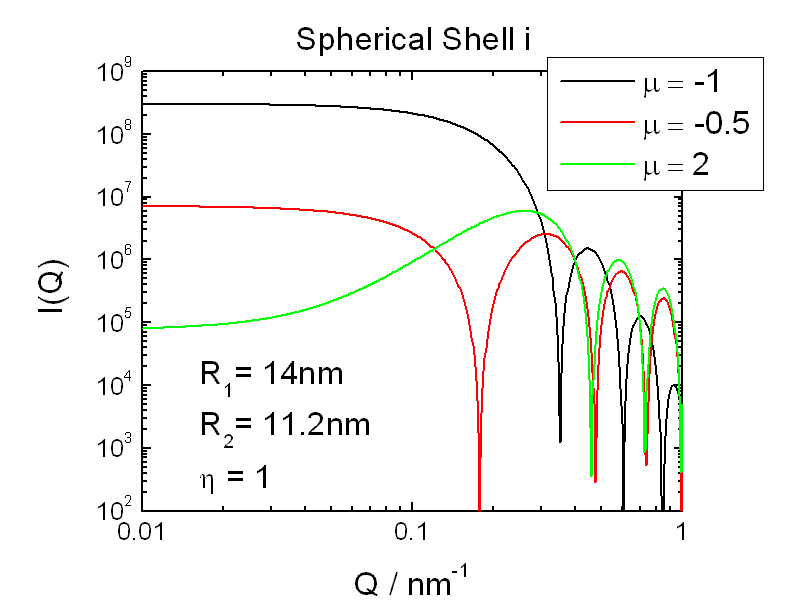
\includegraphics[width=0.768\textwidth,height=0.588\textwidth]{../images/form_factor/spheres/shell_i_P.png}
\end{center}
\caption{Scattering intensity of spherical shell with outer radius of $R_1=14$nm
and inner radius of $R_2=11.2$nm. The scattering length density contrast the shell is set to 1
and the one of the core to -1, -0.5, and 2.} \label{fig:I_shell_i}
\end{figure}


%%%%%%%%%%%%%%%%%%%%%%%%%%%%%%%%%%%%%%%%%%%%%%%%%%%%%%%%%%%
\clearpage
\subsection{Spherical Shell ii}
\label{sect:spherical_shell_ii} ~\\

\begin{figure}[htb]
\begin{center}
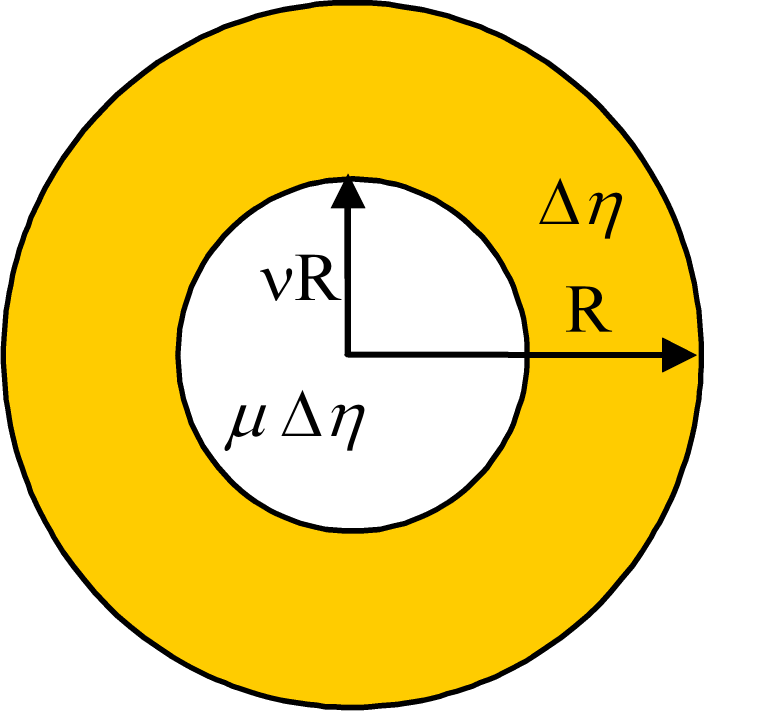
\includegraphics[width=0.38\textwidth,height=0.3575\textwidth]{../images/form_factor/spheres/shell2.png}
\end{center}
\caption{\texttt{Spherical Shell ii}} \label{fig:shell2}
\end{figure}
This implementation of a spherical shell is parametrised with an outer radius $R$ and an inner
radius $\nu R$. The scattering contrast relative to the matrix of the core is $ \mu \Delta \eta$
and the one of the shell $\Delta\eta$.
\begin{align}
I_\text{Shell2}(Q,R,\nu,\Delta\eta,\mu)=
\left(K(Q,R,\Delta\eta)-K(Q,\nu R,\Delta\eta(1-\mu))\right)^2
\end{align}
with
\begin{align}
 K(Q,R,\Delta\eta) = \frac{4}{3}\pi R^3 \Delta\eta \, 3 \frac{\sin QR - QR \cos QR}{(QR)^3}
\end{align}
The forward scattering for $Q=0$ is given by
$$
\DS \lim_{Q=0}I_\text{Shell2}(Q,R,R,\Delta\eta,\mu) =
\left(\frac{4}{3}\pi \Delta\eta \left[ R^3 - \nu^3
R^3(1-\mu)\right]\right)^2
$$

\vspace{5mm}
\noindent \underline{Input Parameters for model \texttt{Spherical Shell ii}:}
\begin{description}
\item[\texttt{R}] overall radius of spherical shell $R$
\item[\texttt{nu}] the radius of the core is only the fraction $\nu$ of the overall radius  $R$
\item[\texttt{eta}] scattering length density difference between shell and matrix $\Delta\eta$
\item[\texttt{mu}] scattering length density difference between core and matrix relative to the shell contrast $\mu$
\end{description}

\noindent\underline{Note:}
\begin{itemize}
\item[~] None
\end{itemize}

\begin{figure}[htb]
\begin{center}
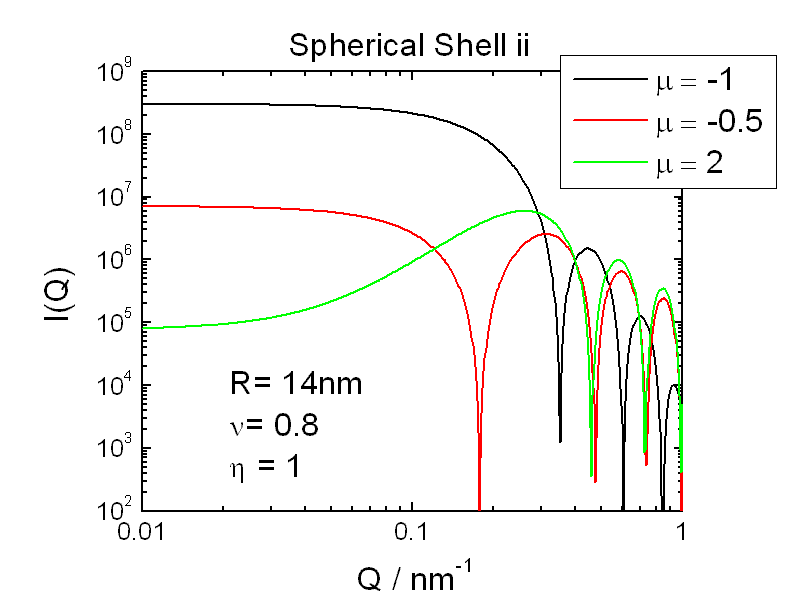
\includegraphics[width=0.768\textwidth,height=0.588\textwidth]{../images/form_factor/spheres/shell_ii_P.png}
\end{center}
\caption{Scattering intensity of spherical shell with outer radius of $R=14$nm
and inner radius of $\nu R=11.2$nm. The scattering length density contrast the shell is set to 1
and the one of the core to -1, -0.5, and 2.} \label{fig:I_shell_ii}
\end{figure}

%%%%%%%%%%%%%%%%%%%%%%%%%%%%%%%%%%%%%%%%%%%%%%%%%%%%%%%%%%%%%%%
\clearpage
\subsection{Spherical Shell iii}
\label{sect:spherical_shell_iii} ~\\

\begin{figure}[htb]
\begin{center}
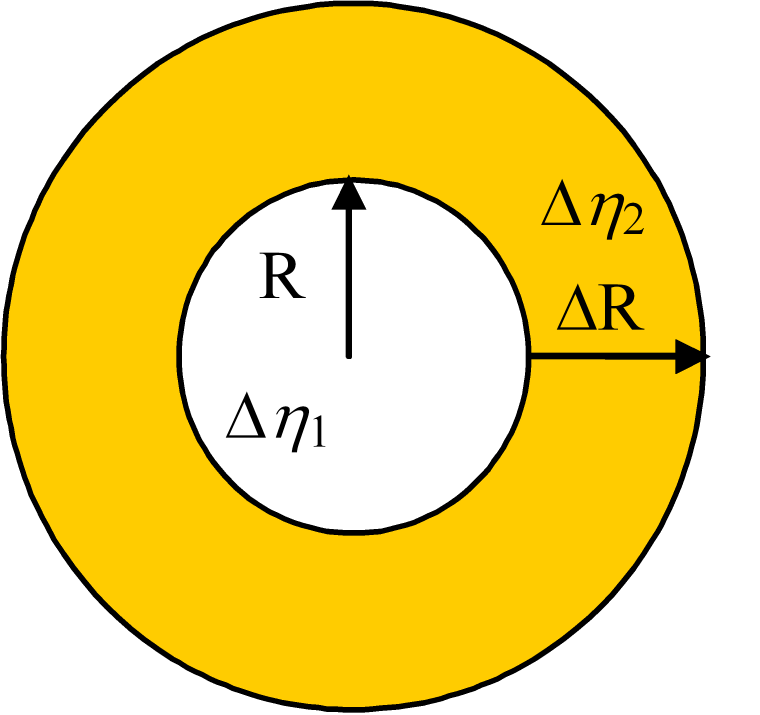
\includegraphics[width=0.38\textwidth,height=0.3575\textwidth]{../images/form_factor/spheres/shell3.png}
\end{center}
\caption{Spherical Shell iii} \label{fig:shell3}
\end{figure}
This implementation of a spherical shell is parametrised with an inner radius $R$ and a shell
thickness $\Delta R$. The scattering contrast relative to the matrix of the core is $ \Delta \eta_1$
and the one of the shell $\Delta\eta_2$.
\begin{align}
I_\text{Shell3}(Q,R,\Delta R,\Delta\eta_1,\Delta\eta_2)=
\left[K(Q,R+\Delta
R,\Delta\eta_2)-K(Q,R,\Delta\eta_2-\Delta\eta_1)\right]^2
\end{align}
with
\begin{align}
 K(Q,R,\Delta\eta) = \frac{4}{3}\pi R^3 \Delta\eta \, 3 \frac{\sin QR - QR \cos QR}{(QR)^3}
\end{align}
The forward scattering for $Q=0$ is given by
$$
\DS \lim_{Q=0}I_\text{Shell3}(Q,R,\Delta R,\Delta\eta_1,\Delta\eta_2)
= \left(\frac{4}{3}\pi \left[(R+\Delta R)^3\Delta\eta_2
                            - R^3(\Delta\eta_2-\Delta\eta_1)\right]\right)^2
$$

\vspace{5mm}
\noindent  \underline{Input Parameters for model \texttt{Spherical Shell iii}:}
\begin{description}
\item[\texttt{R}] radius of core $R$
\item[\texttt{dR}] thickness of the shell $\Delta R$
\item[\texttt{eta1}] scattering length density difference between core and matrix $\Delta\eta_1$
\item[\texttt{eta2}] scattering length density difference between shell and matrix $\Delta\eta_2$
\end{description}

\noindent\underline{Note:}
\begin{itemize}
\item[~] None
\end{itemize}


\begin{figure}[htb]
\begin{center}
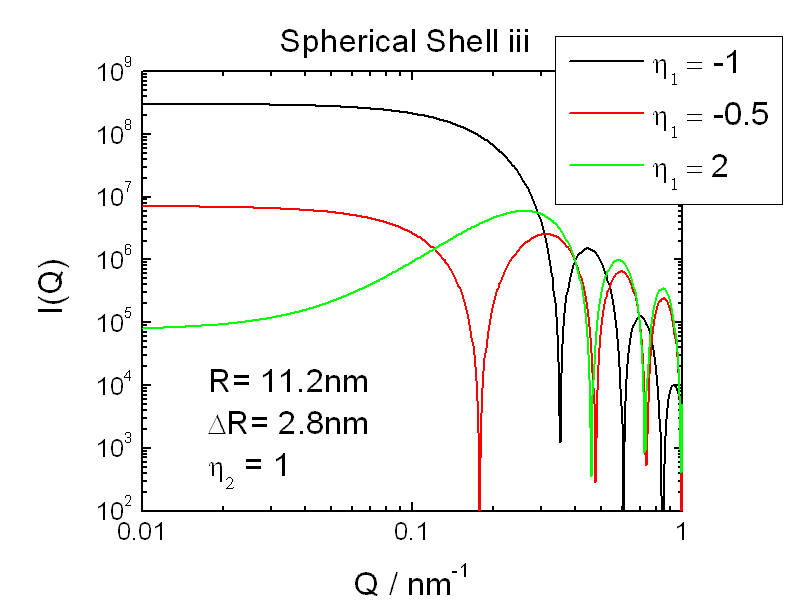
\includegraphics[width=0.768\textwidth,height=0.588\textwidth]{../images/form_factor/spheres/shell_iii_P.png}
\end{center}
\caption{Scattering intensity of spherical shell with core radius of $R=11.2$nm
and shell thickness of $\Delta R=2.8$nm. The scattering length density contrast the shell is set to 1
and the one of the core to -1, -0.5, and 2.} \label{fig:I_shell_iii}
\end{figure}
\clearpage


%%%%%%%%%%%%%%%%%%%%%%%%%%%%%%%%%%%%%%%%%%%%%%%%%%%%%%%%%%%%%%%%%%%%%%%%%%

\clearpage
\subsection{Bilayered Vesicle}
\label{sect:BilayeredVesicle} ~\\

\begin{figure}[htb]
\begin{center}
\includegraphics[width=0.5441\textwidth,height=0.5858\textwidth]{../images/form_factor/spheres/BiLayeredVesicle.png}
\end{center}
\caption{BiLayeredVesicle} \label{fig:BiLayeredVesicle}
\end{figure}
\begin{align}
I_\text{BLV}(Q) = \bigg( & + K(Q,R_c,\eta_{sol}-\eta_{t})+ K(Q,R_c+t_{t},\eta_{t}-\eta_{h}) \\
&+ K(Q,R_c+t_{t}+t_{h},\eta_{h}-\eta_{t}) +
K(Q,R_c+2t_{t}+t_{h},\eta_{t}-\eta_{sol}) \bigg)^2 \nonumber
\end{align}
with
\begin{align}
 K(Q,R,\Delta\eta) = \frac{4}{3}\pi R^3 \Delta\eta \, 3 \frac{\sin QR - QR \cos QR}{(QR)^3}
\end{align}

\vspace{5mm}
\hspace{1pt}\\
\underline{Input Parameters for model \texttt{BilayeredVesicle}:}\\
\begin{description}
\item[\texttt{R\_c}] radius of core $R_c$ which consists of solvent
\item[\texttt{t\_h}] thickness of outer part of bilayer (in contact with solvent, head group) $t_\text{h}$
\item[\texttt{t\_t}] thickness of inner part of bilayer (tail group) $t_\text{t}$
\item[\texttt{eta\_sol}] scattering length density of solvent $\eta_\text{sol}$
\item[\texttt{eta\_h}] scattering length density of outer part of bilayer $\eta_\text{h}$
\item[\texttt{eta\_t}] scattering length density of inner part of bilayer $\eta_\text{t}$
\end{description}

\noindent\underline{Note:}
\begin{itemize}
\item[~] None
\end{itemize}

\begin{figure}[htb]
\begin{center}
\includegraphics[width=0.768\textwidth,height=0.588\textwidth]{../images/form_factor/spheres/bilayered_vesicle.png}
\end{center}
\caption{Scattering intensity of a bilayered vesicle. The scattering intensity has been calculated
with a lognormal $[\mathrm{LogNorm}(N\!=\!1,\sigma\!=\!0.05,p\!=\!1,R\!=\!30)]$ size distribution for the vesicle radius $R_c$.}
\label{fig:I_BiLayeredVesicle}
\end{figure}

%%%%%%%%%%%%%%%%%%%%%%%%%%%%%%%%%%%%%%%%%%%%%%%%%%%%%%%%%%%%%%%%%%

\clearpage
\subsection{Multi Lamellar Vesicle}
\label{sect:MultiLamellarVesicle} ~\\

\begin{figure}[htb]
\begin{center}
\includegraphics[width=0.537\textwidth,height=0.566\textwidth]{../images/form_factor/spheres/multilamellar_vesicle.png}
\end{center}
\caption{MultiLamellarVesicle} \label{fig:MultiLamellarVesicle}
\end{figure}
\begin{align}
I_\text{MLV}(Q) = \Bigg( \sum_{i=0}^{n-1} \bigg[ & K(Q,R_c+it_{sh}+it_{sol},\eta_{sol}-\eta_{sh}) \nonumber \\
+ &K(Q,R_c+(i+1)t_{sh}+it_{sol},\eta_{sh}-\eta_{sol}) \bigg]
\Bigg)^2
\end{align}
with
\begin{align}
 K(Q,R,\Delta\eta) = \frac{4}{3}\pi R^3 \Delta\eta \, 3 \frac{\sin QR - QR \cos QR}{(QR)^3}
\end{align}


\noindent\underline{Input Parameters for model \texttt{MultiLamellarVesicle}:}
\begin{description}
\item[\texttt{R\_c}] radius of core $R_c$ which consists of solvent
\item[\texttt{t\_sh}] surfactant layer thickness $t_\text{sh}$
\item[\texttt{t\_sol}] thickness of solvent layer $t_\text{sol}$
\item[\texttt{eta\_sh}] scattering length density of surfactant layer $\eta_\text{sh}$
\item[\texttt{eta\_sol}] scattering length density of solvent $\eta_\text{sol}$
\item[\texttt{n}] total number of surfactant layers $n$
\end{description}

\noindent\underline{Note:}
\begin{itemize}
\item[~] None
\end{itemize}


\begin{figure}[htb]
\begin{center}
\includegraphics[width=0.768\textwidth,height=0.588\textwidth]{../images/form_factor/spheres/multilamellar_vesicle_Iq.png}
\end{center}
\caption{Scattering intensity of a multilamellar vesicle. The scattering intensities has been calculated
for a\&b) a distribution of the core radius $R_c$ by
$\int\mathrm{LogNorm}(R_c;N\!=\!1,\sigma\!=\!0.3,p\!=\!1,R\!=\!10) I(q,R_c)\, \mathrm{d}R_c$
and c) for a distribution of the distances between the lamellars
$\int\mathrm{LogNorm}(t_\text{sol};N\!=\!1,\sigma\!=\!0.3,p\!=\!1,R\!=\!10) I(q,t_\text{sol})\, \mathrm{d}t_\text{sol}$.}
\label{fig:I_MLV}
\end{figure}

%%%%%%%%%%%%%%%%%%%%%%%%%%%%%%%%%%%%%%%%%%%%%%%%%%%%%%%%%%%%%%%%%%

\clearpage
\subsection{RNDMultiLamellarVesicle}
\label{sect:MultiLamellarVesicle} ~\\

\begin{figure}[htb]
\begin{center}
\includegraphics[width=0.537\textwidth,height=0.566\textwidth]{../images/form_factor/spheres/random_multilamellar_vesicle.png}
\end{center}
\caption{randomMultiLamellarVesicle}
\label{fig:randomMultiLamellarVesicle}
\end{figure}
\begin{align}
I_\text{RndMLV}(Q) &= \Delta\eta ^2 \sum_{i=1}^{N} F_i^2(q,R_i,t_{sh,i}) \nonumber \\
&+ \Delta\eta ^2 \sum_{i<j}^{N} 2 F_i(q,R_i,t_{sh,i}) F_j(q,R_j,t_{sh,j}) \frac{\sin qr_{ij}}{qr_{ij}}
\end{align}
with
\begin{subequations}
\begin{align}
r_{ij} & = \abs{\mathbf{R}_i-\mathbf{R}_j} \\
F_i(q,R_i,t_{sol,i}) &= K(q,R_i+t_{sol,i},\Delta\eta)-K(q,R_i,\Delta\eta)\\
K(q,R,\Delta\eta) &= \frac{4}{3}\pi R^3 \Delta\eta \, 3 \frac{\sin qR - qR \cos qR}{(qR)^3}
\end{align}
\end{subequations}

\begin{subequations}
\begin{align}
R_1 &= \textrm{ran}_{lognormal}\left(\log(R_c),\sigma_{R_c}\right) \\
\Delta R_{i} &= \textrm{ran}_{gaussian}\left(\sigma_{t_{sol}}\right) \\
R_i &= R_{i-1}+t_{sh,i-1}+\Delta R_{i}\\
\mathbf{R}_i &= R_i \; \textbf{ran}_{dir,3D}
                       \text{ran}_{uniform} \; \Delta t_{sol}
\end{align}
\end{subequations}


\hspace{1mm}\\
\underline{Input Parameters for model
\texttt{RNDMultiLamellarVesicle}:}
\begin{description}
\item[\texttt{t\_sh}] average surfactant layer thickness $t_\text{sh}$
\item[\texttt{s\_sh}] Gaussian thickness distribution of surfactant layer with a width of $\sigma_\text{sh}$
\item[\texttt{R\_c}] average radius of core $R_c$ which consists of solvent
\item[\texttt{s\_c}] lognormal size distribution of core radius $R_c$ with a width of $\sigma_c$
\item[\texttt{n}] average number of surfactant layers $n$
\item[\texttt{s\_n}] lognormal distribution of the number of surfactant layers with a width of $\sigma_n$
\item[\texttt{t\_sol}] average thickness of solvent layer $t_\text{sol}$
\item[\texttt{s\_sol}] lognormal thickness distribution of solvent layer with a width of $\sigma_\text{sol}$
\item[\texttt{Deta\_sh}] scattering length density contrast $\Delta\eta$ between surfactant layer and solvent
\end{description}

\noindent\underline{Note:}
\begin{itemize}
\item[~] The number of Monte Carlo iterations can be set via the menu \texttt{[Options|Customize...]}
\end{itemize}

\begin{figure}[htb]
\begin{center}
\includegraphics[width=0.768\textwidth,height=0.588\textwidth]{../images/form_factor/spheres/random_multilamellar_vesicle_Iq.png}
\end{center}
\caption{Scattering intensity of a multilamellar vesicle where several distribution of parameters
within a single vesicle are calculated via a Monte Carlo algorithm. .}
\label{fig:I_rndMLV}
\end{figure}
%%%%%%%%%%%%%%%%%%%%%%%%%%%%%%%%%%%%%%%%%%%%%%%%%%%%%%%%%%%%%%%%%%

\clearpage
\subsection{Vesicle with aligned flat capped ends \cite{Kaya:aj5008,Kaya:aj5016}}
\label{sect:vesicle_capped_poles_aligned} ~\\

\begin{figure}[htb]
\begin{center}
\includegraphics[width=0.492\textwidth,height=0.523\textwidth]{vesicle_capped_poles_aligned.png}
\end{center}
\caption{Sketch of a vesicle with horizontally aligned flat
capped ends perpendicular to the incoming neutron beam}
\label{fig:Sketch_vesicle_capped_poles_aligned}
\end{figure}
The shape of this form factor consist of spherical vesicle containing to flat domains.
The flat thought to be aligned in a horizontal magnetic field perpendicular to the incoming
neutron beam. The size of the domains are characterized by the angles $\theta_1$ and
$theta_2$. The thicknesses $t_{c1}$ and $t_{c2}$ can be different than the thickness $t_{sh}$
of the spherical part of the vesicles. The same hold for the scattering length densities
$\eta_{c1}$, $\eta_{c2}$ and $\eta_{sh}$. The form factor $F_\text{cv}(Q)$ of this object can be
calculated by performing the Fourier transformation of the scattering length density in separate
steps. First one calculates the Fourier transformation of a sphere $F_\text{cSph}$
with flat capped ends on each side in cylinder coordinates.
\begin{subequations}
\begin{align}
F_\text{cSph}(Q,R,\psi,\theta_1,\theta_2,\Delta\eta) = \Delta\eta \!\!
\int_{-R\cos\theta_2}^{R\cos\theta_1} \!\!\!\!\! \mathrm{d}z \!\!\!
\int_0^{\sqrt{R^2-z^2}}\!\!\!\!\! \mathrm{d}\rho \;
\int_0^{2\pi} \mathrm{d}\phi \;\; e^{\imath \mathbf{Q}\cdot\mathbf{r}}
\, \rho
\label{eq:FcSphInt}
\end{align}
\begin{align}
\text{with} \quad
\mathbf{Q}=Q\left(
              \begin{array}{c}
                0 \\
                \sin\psi \\
                \cos\psi
              \end{array}
            \right)
\quad \text{and} \quad
\mathbf{r}= \left(
              \begin{array}{c}
                \rho \cos\phi \\
                \rho \sin\phi \\
                z
              \end{array}
            \right)
\end{align}
\end{subequations}
The form factor of vesicle $F_\text{cv}(Q)$ with a layer thickness of $t_\text{sh}$ can than
be calculated by
\begin{subequations}
\begin{align}
F_\text{cv}(Q,R,t_\text{sh},\theta_1,\theta_2,\Delta\eta_\text{sh}) =
    & + F_\text{cSph}(Q,R+t_\text{sh},\Theta_1,\Theta_2,\Delta\eta_\text{sh}) \nonumber \\
    & - F_\text{cSph}(Q,R,            \theta_1,\theta_2,\Delta\eta_\text{sh})
\end{align}
with
\begin{align}
\Theta_1 &= \arcsin\left(\frac{R_{c1}}{R+t_\text{sh}} \right), \quad R_{c1} = R \sin\left(\theta_1\right),\\
\Theta_2 &= \arcsin\left(\frac{R_{c2}}{R+t_\text{sh}} \right), \quad R_{c2} = R \sin\left(\theta_2\right).
\end{align}
\end{subequations}
As the flat capped ends are allowed to have independent thicknesses $t_\text{c1}$, $t_\text{c2}$ and
scattering length densities $\eta_\text{1}$, $\eta_\text{2}$ the scattering amplitude contribution of the
flat capped ends, which have the shape of a disc, need to be corrected. Their contribution can be calculated by
\newlength\breite
\settowidth\breite{$\displaystyle {}+{}$}
\begin{multline}
\begin{split}
F_\text{c}(Q,R,\theta_1,\theta_2,\dots) =
& \hspace{\breite} F_\text{c1}(Q,R,\theta_1,\Delta\eta_\text{c1}) - F_\text{d1}(Q,R,t_\text{d1},\Delta\eta_\text{sh}) \\
& +                F_\text{c2}(Q,R,\theta_2,\Delta\eta_\text{c2}) - F_\text{d2}(Q,R,t_\text{d2},\Delta\eta_\text{sh})
\end{split} \\[2mm]
\begin{split}
= & \hspace{\breite} \Delta\eta_\text{c1} \!\!\!
\int_{l_\text{c1}}^{l_\text{c1}+t_\text{c1}} \!\!\!\!\!
\mathrm{d}z\int_0^{R_\text{c1}} \!\!  \mathrm{d}\rho \int_0^{2\pi}\!\! \mathrm{d}\phi \; e^{\imath \mathbf{Q}\cdot\mathbf{r}}
\, \rho
- \Delta\eta_\text{sh} \!\!\!
\int_{l_\text{c1}}^{l_\text{c1}+t_\text{d1}} \!\!\!\!\!
\mathrm{d}z\int_0^{R_\text{c1}} \!\! \mathrm{d}\rho \int_0^{2\pi}\!\! \mathrm{d}\phi \; e^{\imath \mathbf{Q}\cdot\mathbf{r}}
\, \rho  \\
& + \Delta\eta_\text{c2} \!\!\!\!\!\!\!
\int_{-(l_\text{c2}+t_\text{c2})}^{-l_\text{c2}} \!\!\!\!\!\!\!\!
\mathrm{d}z\int_0^{R_\text{c2}} \!\! \mathrm{d}\rho \int_0^{2\pi}\!\!\mathrm{d}\phi \; e^{\imath \mathbf{Q}\cdot\mathbf{r}}
\, \rho
- \Delta\eta_\text{sh} \!\!\!\!\!\!\!
\int_{-(l_\text{c2}+t_\text{d2})}^{-l_\text{c2}} \!\!\!\!\!\!\!\!
\mathrm{d}z\int_0^{R_\text{c2}} \!\! \mathrm{d}\rho  \int_0^{2\pi}\!\!\mathrm{d}\phi \; e^{\imath \mathbf{Q}\cdot\mathbf{r}}
\, \rho \label{eq:Fc}
\end{split}
\end{multline}
with
\begin{subequations}
\begin{align}
\Delta\eta_\text{sh} &= \eta_\text{sh}-\eta_\text{sol}, \, \Delta\eta_\text{c1} = \eta_1-\eta_\text{sol} , \,
\Delta\eta_\text{c2} = \eta_2-\eta_\text{sol} \\
l_\text{c1} &= R\cos{\theta_1}, \, l_\text{c2} = R\cos{\theta_2} \\
R_\text{c1} &= R\sin{\theta_1}, \, R_\text{c2} = R\sin{\theta_2} \\
t_\text{d1} &= \sqrt{\left(R+t_\text{sh}\right)^2-R_\text{c1}^2}-\sqrt{R^2-R_\text{c1}^2} \\
t_\text{d2} &= \sqrt{\left(R+t_\text{sh}\right)^2-R_\text{c2}^2}-\sqrt{R^2-R_\text{c2}^2} \\
\end{align}
\end{subequations}
The solution of the integrals in eq.\ \ref{eq:FcSphInt} and \ref{eq:Fc} are
\begin{subequations}
\begin{multline}
F_\text{cSph}(Q,R,\psi,\theta_1,\theta_2,\Delta\eta) = \Delta\eta \!\!
\int_{-R\cos\theta_2}^{R\cos\theta_1} \!\!\!\!\! \mathrm{d}z \!\!\!
\int_0^{\sqrt{R^2-z^2}}\!\!\!\!\! \mathrm{d}\rho \;
\int_0^{2\pi} \mathrm{d}\phi \;\; e^{\imath \mathbf{Q}\cdot\mathbf{r}}
\, \rho  \\
 \Delta\eta \!\!
\int_{-R\cos\theta_2}^{R\cos\theta_1} \!\!\!\!\! \mathrm{d}z\;\;
\exp\left(\imath Q z \cos\psi\right)  2\pi \left(R^2 - z^2\right)
\frac{J_1\left(Q \sqrt{R^2 - z^2} \sin\psi\right)}{Q \sqrt{R^2 - z^2} \sin\psi}
\label{eq:FcSphPsi}
\end{multline}
and
\begin{multline}
F_\textrm{c$_i$,d$_i$}(Q,R_\textrm{c$_i$,d$_i$},\psi,\Delta\eta)   =
\Delta\eta \int_{a}^{b}\!\! \mathrm{d}z
           \int_0^{R_\textrm{c$_i$}}\!\! \mathrm{d}\rho
           \int_0^{2\pi}\!\! \mathrm{d}\phi \;\; e^{\imath \mathbf{Q}\cdot\mathbf{r}}
\, \rho \\
 = 4 \pi R \frac{\imath \left(\exp\left(\imath a Q \cos\psi\right)-\exp\left(\imath b Q \cos\psi\right)\right)
 J_1\left(Q R \sin\psi\right)}{\sin\left(2\psi\right) Q^2}
\end{multline}
\end{subequations}
whereby $\mathrm{J}_1$ the regular cylindrical Bessel function of first order.
The overall scattering intensity $I_{\textrm{alignedVes}}(Q,\psi,\dots)$ is finally given by
\begin{align}
I_{\textrm{alignedVes}}(Q,\psi,\dots) =
\abs{
 F_\text{cv}(Q,R,\psi,t_\text{sh},\theta_1,\theta_2,\Delta\eta_\text{sh})
+F_\text{c}(Q,R,\psi,\theta_1,\theta_2,\dots)}^2
\end{align}
\vspace{5mm}
\begin{sloppypar}
\noindent \underline{Input Parameters for the models of \texttt{MagneticFieldAlignedVesicle}:}
\end{sloppypar}
\begin{description}
\item[\texttt{Rsh}] radius of spherical vesicle shell
\item[\texttt{theta1}] angle to describe size of first capped side
\item[\texttt{theta2}] angle to describe size of second capped side
\item[\texttt{t\_sh}] thickness of spherical vesicle shell
\item[\texttt{t\_c1}] thickness of first flat capped side
\item[\texttt{t\_c2}] thickness of second flat capped side
\item[\texttt{eta\_sh}] scattering length density of spherical vesicle shell
\item[\texttt{eta\_1}] scattering length density of first capped side
\item[\texttt{eta\_2}] scattering length density of second capped side
\item[\texttt{eta\_sol}] scattering length density of solvent
\end{description}

\noindent\underline{Note:}
\begin{itemize}
\item[~] None
\end{itemize}

\begin{figure}[htb]
\begin{center}
%\includegraphics[width=0.768\textwidth,height=0.588\textwidth]{sphere_P.png}
\end{center}
%\caption{Scattering intensity of spheres with radii $R=10$nm and $R=20$nm.
%The scattering length density contrast is set to 1.} \label{fig:I_sphere}
\end{figure}

%%%%%%%%%%%%%%%%%%%%%%%%%%%%%%%%%%%%%%%%%%%%%%%%%%%%%%%%%%%%%%%%%%%%%%%%%%%%%%%%

\clearpage
\subsection{Spherical shell with linear varying contrast profile (LinShell)}
\label{sect:LinShell} ~\\

\begin{figure}[htb]
\begin{center}
\includegraphics[width=0.5\textwidth,height=0.533\textwidth]{../images/form_factor/spheres/linshell.png}
\end{center}
\caption{Form factor of a spherical shell with a core radius $R$
and a shell thickness of $\Delta R$ and a linear varying contrast
profile.} \label{linshell}
\end{figure}

Form factor of a spherical shell with a core radius $R$ and a
shell thickness of $\Delta R$. Here a linear contrast profile
within the shell has been assumed.

\begin{align}
\Delta\eta(r)      & =
\begin{cases}
\eta_\text{c}-\eta_\text{sol} & \text{~for~} r<R \\
m r + b  & \text{~for~} r \in [R,R+\Delta R] \\
0  & \text{~for~} r>R+\Delta R
\end{cases}\\
m           & = (\eta_\text{sh\_out}-\eta_\text{sh\_in}) / \Delta R \\
b           & = -m R + \eta_\text{sh\_in} - \eta_\text{sol} \\
\eta_\text{sh\_in}  & = (1 - x_\text{in,sol})  \, \eta_\text{sh} + x_\text{in,sol} \,\eta_\text{sol}-\eta_\text{sol} \\
                    & : \text{scattering length density at $R$} \nonumber \\
\eta_\text{sh\_out} & = (1 - x_\text{out,sol}) \, \eta_\text{sh} + x_\text{out,sol}\,\eta_\text{sol}-\eta_\text{sol} \\
                    & : \text{scattering length density at $R+\Delta R$} \nonumber \\
\eta_\text{sh}      & : \text{scattering length density of pure shell material} \nonumber \\
\eta_\text{c}       & : \text{scattering length density of core} \nonumber \\
\nonumber
\end{align}

\begin{align}
F_\text{sph}(A,x) & = \frac{4}{3}\pi x^3 \,\, 3\frac{\sin(A)-A\cos(A)}{A^3} \\[5mm]
F_\text{shlin}(A,x) & = 4\pi x^4 \frac{2\cos(A)+2A\sin(A)-A^2\cos(A)}{A^4} \\[5mm]
I_\text{LinShell}    & = \big[ \,\, (\eta_\text{c}-\eta_\text{sol}-b)F_\text{sph}(QR,R) \nonumber \\
             & \hspace{6mm} - mF_\text{shlin}(QR,R) \\
             & \hspace{6mm} + mF_\text{shlin}\left(Q(R+\Delta R),R+\Delta R\right) \nonumber \\
             & \hspace{6mm} + bF_\text{sph}\left(Q(R+\Delta R),R+\Delta R\right) \big]^2 \nonumber
\end{align}

\vspace{5mm}

\underline{Input Parameters for model \texttt{LinShell}:}\\
\begin{description}
\item[\texttt{R}] radius of core $R$
\item[\texttt{dR}] thickness of the shell $\Delta R$
\item[\texttt{eta\_c}] scattering length density $\eta_\text{c}$
\item[\texttt{eta\_sh}] scattering length density of non-swollen shell $\eta_\text{sh}$
\item[\texttt{x\_in}] amount of solvent $x_\text{in,sol}$ on core-shell interface at $R$
\item[\texttt{x\_out}] amount of solvent $x_\text{out,sol}$ on shell-solvent interface at $R+\Delta R$
\item[\texttt{eta\_sol}] scattering length density of solvent $\eta_\text{sol}$
\end{description}

\noindent\underline{Note:}
\begin{itemize}
\item $x_\text{in,sol}$ and $x_\text{out,sol}$ are only physical for values between 0 and 1.
\end{itemize}


\begin{figure}[htb]
\begin{center}
\includegraphics[width=0.768\textwidth,height=0.588\textwidth]{../images/form_factor/spheres/linshell1_Iq.png}
\end{center}
\caption{Scattering intensity of spheres with radius $R=30$nm, a shell thickness
of $\Delta R=10$nm, whereby the shell has a linear profile due to penetration
of solvent into the shell} \label{fig:I_LinShell1}
\end{figure}
%%%%%%%%%%%%%%%%%%%%%%%%%%%%%%%%%%%%%%%%%%%%%%%%%%%%%%%%%%%%%%%%%%%%%%%%%

\clearpage
\subsection{LinShell2}
\label{sect:LinShell2} ~\\

\begin{figure}[htb]
\begin{center}
\includegraphics[width=0.5\textwidth,height=0.533\textwidth]{../images/form_factor/spheres/linshell2.png}
\end{center}
\caption{} \label{linshell}
\end{figure}

Form factor of a spherical shell with a total radius
$R_\text{tot}$ and a shell thickness of $\Delta R$. The definition
are the same than for {\tt LinShell} except that instead of the
core radius $R$ now the total radius $R_\text{tot}$ is used to
parameterize the form factor. The parameter definitions are the
following:

\begin{align}
R&=R_\text{tot}-\Delta R \\
\Delta\eta(r)      & =
\begin{cases}
\eta_\text{c}-\eta_\text{sol} & \text{~for~} r<R \\
m r + b  & \text{~for~} r \in [R,R_\text{tot}] \\
0 & \text{~for~} r>R_\text{tot}
\end{cases}
\\
m           & = (\eta_\text{sh\_out}-\eta_\text{sh\_in}) / \Delta R \\
b           & = -m R + \eta_\text{sh\_in} - \eta_\text{sol} \\
\eta_\text{sh\_in}  & = (1 - x_\text{in,sol})  \, \eta_\text{sh} + x_\text{in,sol} \,\eta_\text{sol} \\
                    & : \text{scattering length density at $R$} \nonumber \\
\eta_\text{sh\_out} & = (1 - x_\text{out,sol}) \, \eta_\text{sh} + x_\text{out,sol}\,\eta_\text{sol} \\
                    & : \text{scattering length density at $R_\text{tot}=R+\Delta R$} \nonumber \\
\eta_\text{sh}      & : \text{scattering length density of pure shell material} \nonumber \\
\eta_\text{c}       & : \text{scattering length density of core} \nonumber \\
x_\text{in,sol}     & : \text{amount of solvent at $R$} \nonumber \\
x_\text{out,sol}    & : \text{amount of solvent at $R_\text{tot}=R+\Delta R$} \nonumber
\end{align}

\begin{align}
F_\text{sph}(A,x) & = \frac{4}{3}\pi x^3 \,\, 3\frac{\sin(A)-A\cos(A)}{A^3} \\[5mm]
F_\text{shlin}(A,x) & = 4\pi x^4 \frac{2\cos(A)+2A\sin(A)-A^2\cos(A)}{A^4} \\[5mm]
I_\text{LinShell2}    & = \big[ \,\, (\eta_\text{c}-\eta_\text{sol}-b)F_\text{sph}(QR,R) \nonumber \\
             & \hspace{6mm} - mF_\text{shlin}(QR,R) \\
             & \hspace{6mm} + mF_\text{shlin}\left(QR_\text{tot},R_\text{tot}\right) \nonumber \\
             & \hspace{6mm} + bF_\text{sph}\left(QR_\text{tot},R_\text{tot}\right) \big]^2 \nonumber
\end{align}

\vspace{5mm}

\hspace{1pt}\\
\underline{Input Parameters for model \texttt{LinShell2}:}\\
\begin{description}
\item[\texttt{Rtot}] total overall radius $R_\text{tot}$
\item[\texttt{dR}] thickness of the shell $\Delta R$
\item[\texttt{eta\_c}] scattering length density $\eta_\text{c}$
\item[\texttt{eta\_sh}] scattering length density of non-swollen shell $\eta_\text{sh}$
\item[\texttt{x\_in}] amount of solvent $x_\text{in,sol}$ on core-shell interface at $R$ $(x_\text{in,sol} \in [0;1])$
\item[\texttt{x\_out}] amount of solvent $x_\text{out,sol}$ on shell-solvent interface at $R+\Delta R$ $(x_\text{out,sol} \in [0;1])$.
\item[\texttt{eta\_s}] scattering length density of solvent $\eta_\text{sol}$
\end{description}


\noindent\underline{Note:}
\begin{itemize}
\item $x_\text{in,sol}$ and $x_\text{out,sol}$ are only physical for values between 0 and 1.
\end{itemize}

%%%%%%%%%%%%%%%%%%%%%%%%%%%%%%%%%%%%%%%%%%%%%%%%%%%%%%%%%%%%%%%%%%%%%%%%%

\clearpage
\subsection{ExpShell}
\label{sect:ExpShell} ~\\

\begin{figure}[htb]
\begin{center}
\includegraphics[width=0.55\textwidth,height=0.5\textwidth]{../images/form_factor/spheres/ExpShell.png}
\end{center}
\caption{} \label{linshell}
\end{figure}

\noindent
\begin{align}
\eta_\text{ExpShell}(r,R_c,\Delta R,\alpha,\phi_\text{in},\phi_\text{out}) &=
\begin{cases}
\eta_c              & r \leq R_c  \\
\eta_\text{exp}(\frac {r-R_c}{\Delta R})   & R_c < r< R_c+\Delta R \\
\eta_\text{sol}     & r> R_c+\Delta R
\end{cases}
\end{align}
\begin{align}
\eta_\text{exp} (x) &=
\begin{cases}
\eta_\text{sh,in}  +
\left[\eta_\text{sh,out}-\eta_\text{sh,in}\right] x \exp\left( \left[ 1-x \right] \alpha\right)
 & \alpha<0 \\[2mm]
\left[\eta_\text{sh,in}-\eta_\text{sh,out}\right] \left[1-x\right] \exp\left(-{x\alpha}\right) +
 \eta_\text{sh,out}& \alpha \geq 0
\end{cases} \\[2mm]
\eta_\text{sh,in} & = \left[ \phi_\text{in}\,\eta_\text{sol}+ \left( 1-\phi_\text{in} \right)
 \eta_\text{sh} \right] \\
\eta_\text{sh,out} & = \left[ \phi_\text{out}\,\eta_\text{sol}+ \left( 1-\phi_\text{out} \right) \eta_\text{sh} \right]
\end{align}

The scattering intensity for the radial symmetric scattering length density profile $\eta_\text{ExpShell}(r)$
can be calculated analytical. The integral needed to be solved for that is
\begin{equation}
I_\text{ExpShell}(Q) = \int_0^\infty 4\pi r^2 \frac{\sin Qr}{Qr}\, \eta_\text{ExpShell}(r)\, dr
\end{equation}

\begin{align}
R_c &=\text{core radius} \nonumber\\
\Delta R &=\text{shell thickness} \nonumber\\
\eta_\text{sh,in}  & = (1 - \phi_\text{in,sol})  \, \eta_\text{sh} + \phi_\text{in,sol} \,\eta_\text{sol} \\
                    & : \text{scattering length density at $R_c$} \nonumber \\
\eta_\text{sh,out}     & = (1 - \phi_\text{out,sol}) \, \eta_\text{sh} + \phi_\text{out,sol}\,\eta_\text{sol} \\
                        & : \text{scattering length density at $R_c+\Delta R$} \nonumber \\
\eta_\text{sh}      & : \text{scattering length density of pure shell material} \nonumber \\
\eta_\text{c}       & : \text{scattering length density of core} \nonumber \\
\phi_\text{in}     & : \text{amount of solvent  at $R_c$} \nonumber \\
\phi_\text{out}    & : \text{amount of solvent at $R_c+\Delta R$} \nonumber \\
\alpha             & : \text{parameter for exponential diffuse profile of the shell} \\
\nonumber
\end{align}


\vspace{5mm}

\hspace{1pt}\\
\underline{Input Parameters for model \texttt{ExpShell}:}\\
\begin{description}
\item[\texttt{R\_core}] radius of core  $R_c$
\item[\texttt{DR}] thickness of the shell $\Delta R$
\item[\texttt{eta\_core}] scattering length density $\eta_\text{c}$
\item[\texttt{eta\_shell}] scattering length density of non-swollen shell $\eta_\text{sh}$
\item[\texttt{x\_in\_sol}] amount of solvent $\phi_\text{in}$ on core-shell interface at $r=R$
\item[\texttt{x\_out\_sol}] amount of solvent $\phi_\text{out}$ on shell-solvent interface at $r=R+\Delta R$
\item[\texttt{alpha}]  a parameter ($\alpha$) which describes the penetration profile of the solvent into the shell.
A value of $\alpha=0$ means linear profile and is equivalent to {\tt LinShell} and {\tt LinShell2}. For $\alpha>0$
the solvent penetrates further into the shell and for $\alpha<0$ less.
\item[\texttt{eta\_solvent}] scattering length density of solvent $\eta_\text{sol}$
\end{description}

\noindent\underline{Note:}
\begin{itemize}
\item $\phi_\text{in}$ and $\phi_\text{out}$ are only physical for values between 0 and 1.
\end{itemize}

\begin{figure}[htb]
\begin{center}
\includegraphics[width=0.768\textwidth,height=0.588\textwidth]{../images/form_factor/spheres/exp_shell.png}
\end{center}
\caption{Scattering intensity of a spherical shell with an exponential shell profile. The scattering intensity has been calculated
with a lognormal $[\mathrm{LogNorm}(N\!=\!1,\sigma\!=\!0.05,p\!=\!1,R\!=\!30)]$ size distribution for the core radius $R_c$.
The scattering length density of the core $\eta_\text{c}$ and the solvent $\eta_\text{sol}$ are set to 0, $\eta_\text{sh}=1$,
$\phi_\text{in}=0$, and $\phi_\text{out}=1$}
\label{fig:I_BiLayeredVesicle}
\end{figure}

\clearpage
\clearpage
\section{Ellipsoidal Objects}
\label{sect:EllipsoidalObjects}

\subsection{Ellipsoid with two equal semi-axis $R$ and semi-principal axes $\nu R$}
\label{sect:Ellipsoid_ii} ~\\


\begin{figure}[htb]
\begin{center}
%\includegraphics[width=0.706\textwidth,height=0.346\textwidth]{Elpsminr.png}
\includegraphics[width=0.5\textwidth,height=0.245\textwidth]{../images/form_factor/Ellipsoid/Elpsminr.png}
\end{center}
\caption{Ellipse, showing major and minor axes and parameters $a$ and $b$}
\label{minormajoraxes}
\end{figure}

An ellipsoid is a quadric surface in three dimensions obtained by
rotating an ellipse about one of its principal axes. Three
particular cases of an ellipsoid are:
\begin{itemize}
\item If the ellipse is rotated about its major axis, the surface is a prolate spheroid.
\item If the ellipse is rotated about its minor axis, the surface is an oblate spheroid.
\item If the generating ellipse is a circle, the surface is a sphere.
\end{itemize}

\begin{figure}[htb]
\begin{center}
\begin{minipage}[b]{0.5\linewidth}
\begin{center}
\includegraphics[width=7.5cm,height=5.7cm]{../images/form_factor/Ellipsoid/OblateSpheroid.png} \\
(a) oblate spheroid ($\nu <1$)
\end{center}
\end{minipage}%
\begin{minipage}[b]{0.5\linewidth}
\begin{center}
\includegraphics[width=5.1cm,height=7.5cm]{../images/form_factor/Ellipsoid/ProlateSpheroid.png}\\
(b) prolate spheroid ($\nu >1$)
\end{center}
\end{minipage}
\end{center}
\caption{A spheroid is an ellipsoid having two equal equatorial semi-axes. If the equatorial
semi-axis are larger than the principal axis the spheroid becomes oblate (a), if they are smaller
it becomes prolate (b) and if they are equal the spheroid becomes a perfect sphere}
\label{prolate oblate}
\end{figure}

\begin{align}
I_\text{ii}(Q,R,\nu) = \left( \frac{4}{3}\pi R^3 \Delta\eta
\right)^2
 \int_0^{\frac{\pi}{2}}\! K^2\left(Q,R\sqrt{\nu^2\cos^2\Theta+\sin^2\Theta}\right) \sin\Theta\, d\Theta
\end{align}
with $\DS \lim_{Q=0} I_\text{ii}(Q,R,\nu)= \left( \frac{4}{3}\pi
\nu R^3 \Delta\eta \right)^2 $

~\\
\underline{Input Parameters for model \texttt{Ellipsoid ii}:}
\begin{description}
\item[\texttt{R}] radius of the rotational axes
\item[\texttt{nu}]
ratio between radius of the semi-principle axes and equatorial axis.
Values of $\nu<1$ describe a oblate ellipsoid, a value of $\nu=1$ a
sphere, and $\nu>1$ a prolate ellipsoid.
\end{description}

\begin{figure}[htb]
\begin{center}
\includegraphics[width=0.768\textwidth,height=0.588\textwidth]{../images/form_factor/Ellipsoid/ellipsoid_ii.png}
\end{center}
\caption{form factor of an ellipsoid with axis $R$, $R$ and $\nu
R$.} \label{fig:I_ellipsoid_ii}
\end{figure}
%%%%%%%%%%%%%%%%%%%%%%%%%%%%%%%%%%%%%%%%%%%%%%%%%%%%%%%%
\clearpage
\subsection{Ellipsoid with two equal equatorial semi-axis $R$ and volume $V$}
\label{sect:Ellipsoid_i} ~\\

\begin{align}
I_\text{i}(Q,R,\nu) = \left( V \Delta\eta
\right)^2
 \int_0^{\frac{\pi}{2}}\! K^2\left(Q,R\sqrt{\nu^2\cos^2\Theta+\sin^2\Theta}\right)\sin\Theta\, d\Theta
\end{align}
with
$$
\nu=\frac{V}{R^3}\frac{3}{4\pi} \quad \mbox{so that}\quad V =\frac{4}{3}\pi\nu R^3
$$
and $\DS \lim_{Q=0} I_\text{i}(Q,R,\nu)= \left(V\Delta\eta\right)^2$

~\\
\underline{Input Parameters for model \texttt{Ellipsoid i}:}
\begin{description}
\item[\texttt{R}] radius of the rotational axes
\item[\texttt{V}] total volume of the ellipsoid.
\end{description}

\begin{figure}[htb]
\begin{center}
\includegraphics[width=0.768\textwidth,height=0.588\textwidth]{../images/form_factor/Ellipsoid/ellipsoid_i.png}
\end{center}
\caption{form factor of an ellipsoid with axis $R$, $R$ and
$\oldsqrt[3]{V\frac{3}{4\pi}}$.} \label{fig:I_ellipsoid_i}
\end{figure}
%%%%%%%%%%%%%%%%%%%%%%%%%%%%%%%%%%%%%%%%%%%%%%%%%%%%%%%%
\clearpage
\subsection{Ellipsoidal core shell structure}
\label{sect:EllipsoidalCoreShell} ~\\

\begin{figure}[htb]
\begin{center}
\includegraphics[width=0.5\textwidth,height=0.28855\textwidth]{ellipsoidalShell.png}
\end{center}
\caption{} \label{ellipsoidalShell}
\end{figure}
\begin{align}
I_\text{ECSh}(Q) = \left\langle F^2(Q,\mu) \right\rangle
& = \int_0^1 \left[F(Q,\mu)\right]^2 d\mu \\
\left\langle F(Q,\mu) \right\rangle^2 & = \left[\int_0^1 F(Q,\mu)
d\mu \right]^2
\end{align}
\begin{align}
F(Q,\mu) &= \left(\eta_\text{c}-\eta_\text{sh}\right) V_c\left[
\frac{3j_1(x_c)}{x_c}\right]
          +\left(\eta_\text{sh}-\eta_\text{sol}\right) V_t\left[ \frac{3j_1(x_t)}{x_t}\right]
          \nonumber \\
j_1(x) &= \frac{\sin(x)-x\cos(x)}{x^2} \nonumber \\
x_c &= Q \sqrt{a^2\mu^2+b^2(1-\mu^2)} \nonumber \\
x_c &= Q \sqrt{(a+t)^2\mu^2+(b+t)^2(1-\mu^2)} \nonumber \\
V_c &= \frac{4}{3}\pi ab^2 \nonumber \\
V_t &= \frac{4}{3}\pi (a+t)(b+t)^2 \nonumber
\end{align}
\begin{align}
\eta_\text{c} &: \text{scattering length density of core} \nonumber \\
\eta_\text{sh} &: \text{scattering length density of shell} \nonumber \\
\eta_\text{sol} &: \text{scattering length density of solvent} \nonumber \\
a &: \text{semi-principal axes of elliptical core} \nonumber \\
b &: \text{equatorial semi-axis of elliptical core} \nonumber \\
t &: \text{thickness of shell} \nonumber \\
V_c &: \text{volume of core} \nonumber \\
V_t &: \text{total volume of core along with shell} \nonumber
\end{align}

\vspace{0.5cm}

\underline{Input Parameters for model \texttt{EllipsoidalCoreShell}:}
\begin{description}
\item[\texttt{a}] semi-principal axes of elliptical core $a$
\item[\texttt{b}] equatorial semi-axis axes of elliptical core $b$
\item[\texttt{t}] thickness of shell $t$
\item[\texttt{eta\_c}] scattering length density of core $\eta_\text{c}$
\item[\texttt{eta\_sh}] scattering length density of shell $\eta_\text{sh}$
\item[\texttt{eta\_sol}] scattering length density of solvent $\eta_\text{sol}$
\end{description}

\begin{figure}[htb]
\begin{center}
\includegraphics[width=0.768\textwidth,height=0.588\textwidth]{../images/form_factor/Ellipsoid/ellipsoidal_core_shell.png}
\end{center}
\caption{form factor of an ellipsoidal core shell $a$, $b$, $b$ and
$t$.} \label{fig:I_ellipsoidal_core_shell}
\end{figure}
%%%%%%%%%%%%%%%%%%%%%%%%%%%%%%%%%%%%%%%%%%%%%%%%%%%%%%%%
\clearpage
\subsection{triaxial ellipsoidal core shell structure}
\label{sect:triaxEllShell1} ~\\

\begin{figure}[htb]
\begin{center}
\includegraphics[width=0.45\textwidth,height=0.32177\textwidth]{../images/form_factor/Ellipsoid/triaxEll.png}
\hspace{0.08\textwidth}
\includegraphics[width=0.45\textwidth,height=0.4096\textwidth]{../images/form_factor/Ellipsoid/A4ellipd.png}
\end{center}
\caption{triaxial ellipsoidal core shell structure} \label{triaEllShell}
\end{figure}

\begin{align}
I_\text{triaxEllSh}(Q) &= \int^1_0 \int ^1_0 dx\,dy\, K_\text{sh}^2(Q,R,R_t)\\
K(QR)         &= 3 \frac{\sin QR - QR\cos QR}{(QR)^3} \\
K_\text{sh}(Q,R,R_t) &= \left(\eta_\text{c}-\eta_\text{sh}\right)K(QR)+\left(\eta_\text{sh}-\eta_\text{sol}\right)K(QR_t) \\
R^2 &= \left[a^2\cos^2\left(\pi x/2\right) + b^2\sin^2\left(\pi x/2\right)\right](1-y^2)+c^2y^2 \nonumber \\
R_t^2 &= \left[(a+t)^2\cos^2\left(\pi x/2\right) + (b+t)^2\sin^2\left(\pi x/2\right)\right](1-y^2)+(c+t)^2y^2
\nonumber \\
V_c &= \frac{4}{3}\pi abc \nonumber \\
V_t &= \frac{4}{3}\pi (a+t)(b+t)(c+t) \nonumber
\end{align}
\begin{align}
\eta_\text{c} &: \text{scattering length density of core} \nonumber \\
\eta_\text{sh} &: \text{scattering length density of shell} \nonumber \\
\eta_\text{sol} &: \text{scattering length density of solvent} \nonumber \\
a &: \text{semi-axes of elliptical core} \nonumber \\
b &: \text{semi-axes of elliptical core} \nonumber \\
c &: \text{semi-axes of elliptical core} \nonumber \\
t &: \text{thickness of shell} \nonumber \\
V_c &: \text{volume of core} \nonumber \\
V_t &: \text{total volume of core along with shell} \nonumber
\end{align}

\vspace{3cm}
\underline{Input Parameters for model \texttt{triaxEllShell1}:}
\begin{description}
\item[\texttt{a}] semi-axes of elliptical core $a$
\item[\texttt{b}] semi-axes of elliptical core $b$
\item[\texttt{c}] semi-axes of elliptical core $c$
\item[\texttt{t}] thickness of shell $t$
\item[\texttt{eta\_c}] scattering length density of core $\eta_\text{c}$
\item[\texttt{eta\_sh}] scattering length density of shell $\eta_\text{sh}$
\item[\texttt{eta\_sol}] scattering length density of solvent $\eta_\text{sol}$
\end{description}

\begin{figure}[htb]
\begin{center}
\includegraphics[width=0.768\textwidth,height=0.588\textwidth]{../images/form_factor/Ellipsoid/triax_ellipsoidal_core_shell.png}
\end{center}
\caption{Form factor of an triaxial ellipsoidal core shell with semi
axis $a$, $b$ and $c$ and a shell thickness $t$.}
\label{fig:I_ellipsoidal_core_shell}
\end{figure}

\clearpage
\section{Polymers and Micelles}
\label{sect:Polymers_Micelles}

\subsection{Gaussian chain}
\label{sect:GaussCoil}
~\\

\begin{figure}[htb]
\begin{center}
\includegraphics[width=0.744\textwidth,height=0.823\textwidth]{Walk3d_0.png}
\end{center}
\caption{The underlying model for a polymer chain is an
isotropic random walk on the euclidean lattice $\mathbb{Z}^3$.
This picture shows three different walks after 10 000 unit steps,
all three starting from the origin. \label{fig:RandomWalk3D}}
\end{figure}

Consider a flexible polymer coil where each monomer located at a
distance $\mathbf{R}_m$ its scattering field amplitude is given by
\begin{align}
F(\mathbf{q},t) &= \sum_{m=1}^N e^{-\imath
\mathbf{q}\cdot\mathbf{R}_m(t)} .
\end{align}
The scattering intensity averaged over all molecule configurations
reads
\begin{align}
\left\langle \abs{F(\mathbf{q})}^2\right\rangle
&= \sum_{m,n} \left\langle e^{-\imath\mathbf{q}\cdot(\mathbf{R}_m-\mathbf{R}_n)} \right\rangle
\end{align}
As the monomer segments $\mathbf{R}_m-\mathbf{R}_n$ are Gaussian distributed
the averages $\langle\cdots\rangle$ can be written as
\begin{subequations}
\begin{align}
\left\langle e^{-\imath\mathbf{q}\cdot(\mathbf{R}_m-\mathbf{R}_n)} \right\rangle
&= e^{\frac{q^2}{6}\left\langle \left( \mathbf{R}_m-\mathbf{R}_n\right)^2\right\rangle} \\
&= e^{-\frac{q^2b^2}{6}\abs{m-n}^{2\nu}}
\end{align}
\end{subequations}
Here $b$ is the statistical segment length and the contour length $L$ equals $L=Nb$.
The average of the segment inter-distances squares is kept in the general form
\begin{align}
\left\langle \left( \mathbf{R}_m-\mathbf{R}_n\right)^2\right\rangle
&= b^2 \abs{m-n}^{2\nu}.
\end{align}
$\nu$ is the excluded volume parameter from the Flory mean field
theory\footnote{P.J. Flory, "Statistical Mechanics of Chain Molecules", Interscience Publishers (1969)}\footnote{\href{http://www.ncnr.nist.gov/staff/hammouda/the_SANS_toolbox.pdf}{Boualem Hammouda, \texttt{the\_SANS\_toolbox.pdf}}}
of polymer solutions. The radius of gyration $R_G$ is given by
\begin{subequations}
\begin{align}
R_G^2 &= \frac{1}{2N^2}\sum_{m,n}^N \left\langle \left( \mathbf{R}_m-\mathbf{R}_n\right)^2\right\rangle \\
      &= \frac{1}{2N^2}\sum_{m,n}^N b^2 \abs{m-n}^{2\nu} \\
      &= \frac{b^2}{N} \sum_k^N \left(1-\frac{k}{N}\right) k^{2\nu} \\
      &= \frac{b^2}{\left(2\nu+1\right)\left(2\nu+2\right)} N^{2\nu}
\end{align}
\end{subequations}
Three cases are relevant:
\begin{enumerate}
\item Self-avoiding walk corresponds to swollen chains with $\nu = 3/5$, for which
$R_G^2=\frac{25}{176}b^2N^{6/5}$.
\item Pure random walk corresponds to chains in $\Theta$-conditions (where solvent-solvent,
monomer-monomer and solvent-monomer interactions are equivalent) with $\nu = 1/2$,
for which $R_G^2=\frac{1}{6}b^2N$.
\item Self attracting walk corresponds to collapsed chains with $\nu = 1/3$, for which
$R_G^2=\frac{9}{40}b^2N^{2/3}$.
\end{enumerate}
Using the general identity
\begin{align}
\sum_{i,j}^N y(\abs{i-j}) = N+2\sum_{k=1}^N(N-k) y(k)
\end{align}
the form factor reads
\begin{align}
P(q) &= \frac{1}{N^2}\abs{F(q)}^2 = \frac{1}{N^2}
\left\{N+2\sum_{k=1}^N(N-k)e^{-\frac{q^2b^2}{6}k^{2\nu}} \right\}
\end{align}
Going to the continuous limit $(N \gg 1)$, one obtains:
\begin{subequations}
\begin{align}
P(q) &= 2\int_0^1 \mathrm{d}x \; (1-x)e^{-\frac{q^2b^2}{6}N^{2\nu}x^{2\nu}} \\
&= \frac{U^{\frac{1}{2 \nu}} \Gamma\left(\frac{1}{2 \nu}\right)-
\Gamma\left(\frac{1}{\nu}\right)-U^{\frac{1}{2\nu}}
\Gamma\left(\frac{1}{2 \nu},U\right)+\Gamma\left(\frac{1}{\nu},U\right)}{\nu U^{1/\nu}} \\
&= \frac{1}{\nu U^{\frac{1}{2 \nu}}} \; \gamma\left(\frac{1}{2 \nu},U\right)-
   \frac{1}{\nu U^{\frac{1}{\nu}}}   \; \gamma\left(\frac{1}{  \nu},U\right)
\label{eq:generalizedGauss}
\end{align}
\end{subequations}
with the modified variable
\begin{align}
U&=\frac{q^2b^2N^{2\nu}}{6} = \left(2\nu+1\right)\left(2\nu+2\right)\frac{q^2R_G^2}{6}
\end{align}
and the upper incomplete Gamma Function $\Gamma(a,x) = \int_x^\infty \mathrm{d}t \; t^{a-1} \exp(-t)$ and lower incomplete Gamma Function $\gamma(a,x) = \int_0^x \mathrm{d}t \; t^{a-1} \exp(-t)$
for $a$ real and $x \geq 0$ and the Gamma function $\Gamma(a)=\Gamma(a,0)=\gamma(a,\infty)= \Gamma(a,x)+\gamma(a,x)=\int_0^\infty \mathrm{d}t\;  t^{a-1} \exp(-t)$.
Polymer chains follow Gaussian statistics in polymer solutions: they are swollen in good
solvents $\nu=3/5$, are thermally relaxed in "theta"-solvents $\nu=1/2$ and partially precipitate in poor solvents $\nu=1/3$.
The familiar Debye function is recovered when $\nu = 1/2$. The asymptotic limit at large $q$-values of the generalized
Gaussian chain is dominated by the $\frac{1}{\nu U^{\frac{1}{2\nu}}}\Gamma\left(\frac{1}{2\nu}\right)$
term which varies like $U^{-1/(2\nu)} \sim q^{-1/\nu}$. For $\nu =1$ we get the limit of an infinitesimal thin rod
and for $\nu=1/4$ a compact object with a Porod law of $q^{-4}$.

\SASfit has implemented the generalized form of a Gaussian (\texttt{generalized Gaussian coil}) coil and the standard
Debye formula \texttt{Gauss}. In both cases three version are implemented which only differ in their parametrization of
the forward scattering. In case of the the Debye-formula also the polydisperse \texttt{GaussPoly} is implemented.

\textcolor[rgb]{1.00,1.00,1.00}{Gauss}\\
\subsubsection{Gauss \cite{Debye1947}}
\label{sect:Gauss}
~\\
Flexible polymer chains which are not self-avoiding
and obey Gaussian statistics. Debye (1947) has calculated the form factor of such
chains:
\begin{align}
I_\text{Gauss}(q) &= I_0 2\frac{\exp(-u)+u-1}{u^2} \label{eq:DebyeGauss}\\
u &= q^2R_g^2
\end{align}

\vspace{5mm}
\underline{Input Parameters for model \texttt{Gauss}:}
\begin{description}
\item[\texttt{Rg}] radius of gyration $R_g$
\item[\texttt{I0}] forward scattering $I_0$ for $q=0$
\end{description}
\vspace{5mm}

\textcolor[rgb]{1.00,1.00,1.00}{Gauss}\\
\subsubsection{Gauss2 \cite{Debye1947}}
\label{sect:Gauss2}
~\\
This form factor differs only by the parametrization for the forward scattering
$I_0=(b_p-V\eta_\text{s})^2$ from the Debye formula in eq.\ \ref{eq:DebyeGauss}
\begin{align}
I_\text{Gauss2}(q) &= \beta^2 2\frac{\exp(-u)+u-1}{u^2} \\
u &= q^2R_g^2 \nonumber \\
\beta &= b_p-V\eta_\text{s}, \nonumber
\end{align}
where $b_p$ is the scattering length of a polymer molecule of molecular volume $V$ dissolved in a solvent
of scattering length density $\eta_\text{s}$ from which the excess scattering length of a polymer molecule
$\beta$ can be calculated. Combining this form factor with a \texttt{Delta} size distribution \ref{sec:Delta}
is needed to scale the scattering intensity. With proper values for the form factor the parameter $N$
of the \texttt{Delta}-distribution yields the particle number density.

\vspace{5mm}
\underline{Input Parameters for model \texttt{Gauss2}:}
\begin{description}
\item[\texttt{Rg}] radius of gyration $R_g$
\item[\texttt{b\_p}] scattering length of polymer $b_p$ in [cm]
\item[\texttt{V}] molecular volume of a single polymer molecule $V$ in [cm$^3$]
\item[\texttt{eta\_s}] scattering length density of solvent $\eta_\text{s}$ in [cm$^{-2}$]
\end{description}

\textcolor[rgb]{1.00,1.00,1.00}{Gauss}\\
\subsubsection{Gauss3 \cite{Debye1947}}
\label{sect:Gauss3}
~\\
This form factor differs only by the parametrization for the forward scattering
$I_0=(b_p-\frac{M_w}{N_a\rho_p}\eta_\text{s})^2$ from the Debye formula in eq.\ \ref{eq:DebyeGauss}
\begin{align}
I_\text{Gauss3}(q) &= \beta^2 2\frac{\exp(-u)+u-1}{u^2}
\end{align}
with
\begin{align}
u &= q^2R_g^2 \nonumber \\
\beta &= b_p-V\eta_\text{s} \nonumber\\
V &= \frac{M_w}{N_a\rho_p} \nonumber \\
N_a &= \mbox{Avogadro number} \nonumber
\end{align}

\underline{Input Parameters for model \texttt{Gauss3}:}
\begin{description}
\item[\texttt{Rg}] radius of gyration $R_g$
\item[\texttt{b\_p}] scattering length of polymer $b_p$ in [cm]
\item[\texttt{M\_w}] molecular weight of polymer $M_w$ in [g/mol]
\item[\texttt{rho\_p}] mass density of polymer $\rho_p$ in [g cm$^{-3}$]
\item[\texttt{eta\_s}] scattering length density of solvent $\eta_\text{s}$ in [cm$^{-2}$]
\end{description}

\begin{figure}[htb]
\begin{center}
\includegraphics[width=0.768\textwidth,height=0.588\textwidth]{gaussian_coils.png}
\end{center}
\caption{Scattering function of Gaussian coils plotted for several radii of gyration.}
\label{fig:I_gaussian_coils}
\end{figure}

\textcolor[rgb]{1.00,1.00,1.00}{Gauss}\\
\subsubsection{Polydisperse flexible polymers with Gaussian statistics \cite{Pedersen2002}}  \label{sect:GaussPoly}
~\\
Polydispersity has been included in terms of a Schulz�Zimm mass distribution by
Zimm (1948) \cite{zimm:1093}  and Greschner (1973) \cite{Greschner1973}
~\\

\begin{align}
I_\text{GaussPoly}(q) &= I_0 2 \frac{\left( 1+U x\right)^{-1/U}+x-1}{(1+U)x^2} \\
x &= q^2R_g^2/(1+2U) \nonumber \\
U &= \frac{M_w}{M_n} -1 \nonumber
\end{align}

\vspace{5mm}
\underline{Input Parameters for model \texttt{GaussPoly}:}
\begin{description}
\item[\texttt{Rg}] radius of gyration $R_g$
\item[\texttt{M\_w}] weight averaged molecular weight $M_w$
\item[\texttt{M\_n}] number averaged molecular weight $M_n$
\item[\texttt{I0}] forward scattering $I_0$ for $q=0$
\end{description}

\begin{figure}[htb]
\begin{center}
\includegraphics[width=0.768\textwidth,height=0.588\textwidth]{gauss_poly.png}
\end{center}
\caption{Scattering function of polydisperse Gaussian coil plotted for several ratios of $M_w/M_n$.}
\label{fig:I_gauss_poly}
\end{figure}

\textcolor[rgb]{1.00,1.00,1.00}{Gauss}\\
\subsubsection{generalalized Gaussian coil \cite{Hammouda,Hammouda2012,Hammouda1993,Hammouda2016}}
\label{sect:generalized_gaussian_coil}
~\\
The scattering function for the generalized Gaussian coil is according to eq.\ \ref{eq:generalizedGauss}
\begin{align}
I_\text{gGc}(q) &= I_0
\left(
\frac{1}{\nu U^{\frac{1}{2 \nu}}} \; \gamma\left(\frac{1}{2 \nu},U\right)-
\frac{1}{\nu U^{\frac{1}{  \nu}}} \; \gamma\left(\frac{1}{  \nu},U\right)
\right)
\label{eq:generalizedGauss1}
\end{align}
with the modified variable
\begin{align}
U&= \left(2\nu+1\right)\left(2\nu+2\right)\frac{q^2R_G^2}{6}
\end{align}
and the lower incomplete Gamma Function $\gamma(a,x) = \int_0^x \mathrm{d}t \; t^{a-1} \exp(-t)$.
$\nu$ is the excluded volume parameter from the Flory mean field theory and typical values for them are
\begin{description}
\item[$\nu=1/3$] partially precipitate in poor solvents
\item[$\nu=1/2$] thermally relaxed in "theta"-solvents
\item[$\nu=3/5$] swollen in good solvents
\end{description}

\vspace{5mm}
\underline{Input Parameters for model \texttt{generalized Gaussian coil}:}
\begin{description}
\item[\texttt{Rg}] radius of gyration $R_g$
\item[\texttt{nu}] excluded volume parameter $\nu\in [1/2;1]$
\item[\texttt{I0}] forward scattering $I_0$ for $q=0$
\end{description}
\vspace{5mm}


\subsubsection{generalized Gaussian coil 2 \cite{Hammouda,Hammouda2012}}
\label{sect:generalized_gaussian_coil2}
~\\
The scattering function for the generalized Gaussian coil is according to eq.\ \ref{eq:generalizedGauss}
and differs only by the parametrization for the forward scattering
$I_0=(b_p-V\eta_\text{s})^2$ from the formula in eq.\ \ref{eq:generalizedGauss1}
\begin{align}
I_\text{gGc2}(q) &= \left(b_p-V\eta_\text{s}\right)^2
\left(
\frac{1}{\nu U^{\frac{1}{2 \nu}}} \; \gamma\left(\frac{1}{2 \nu},U\right)-
\frac{1}{\nu U^{\frac{1}{  \nu}}} \; \gamma\left(\frac{1}{  \nu},U\right)
\right)
\label{eq:generalizedGauss2}
\end{align}
with the modified variable
\begin{align}
U&= \left(2\nu+1\right)\left(2\nu+2\right)\frac{q^2R_G^2}{6}
\end{align}

\vspace{5mm}
\underline{Input Parameters for model \texttt{generalized Gaussian coil 2}:}
\begin{description}
\item[\texttt{Rg}] radius of gyration $R_g$
\item[\texttt{b\_p}] scattering length of polymer $b_p$ in [cm]
\item[\texttt{V}] molecular volume of a single polymer molecule $V$ in [cm$^3$]
\item[\texttt{eta\_s}] scattering length density of solvent $\eta_\text{s}$ in [cm$^{-2}$]
\end{description}
\vspace{5mm}

\subsubsection{generalized Gaussian coil 3 \cite{Hammouda,Hammouda2012}}
\label{sect:generalized_gaussian_coil3}
~\\
The scattering function for the generalized Gaussian coil is according to eq.\ \ref{eq:generalizedGauss}
and differs only by the parametrization for the forward scattering
$I_0=(b_p-\frac{M_w}{N_a\rho_p}\eta_\text{s})^2$ from the formula in eq.\ \ref{eq:generalizedGauss1}
\begin{align}
I_\text{gGc3}(q) &= \left(b_p-\frac{M_w}{N_a\rho_p}\eta_\text{s}\right)^2
\left(
\frac{1}{\nu U^{\frac{1}{2 \nu}}} \; \gamma\left(\frac{1}{2 \nu},U\right)-
\frac{1}{\nu U^{\frac{1}{  \nu}}} \; \gamma\left(\frac{1}{  \nu},U\right)
\right)
\label{eq:generalizedGauss3}
\end{align}
with the modified variable
\begin{align}
U&= \left(2\nu+1\right)\left(2\nu+2\right)\frac{q^2R_G^2}{6}
\end{align}

\vspace{5mm}
\underline{Input Parameters for model \texttt{generalized Gaussian coil 3}:}
\begin{description}
\item[\texttt{Rg}] radius of gyration $R_g$
\item[\texttt{b\_p}] scattering length of polymer $b_p$ in [cm]
\item[\texttt{M\_w}] molecular weight of polymer $M_w$ in [g/mol]
\item[\texttt{rho\_p}] mass density of polymer $\rho_p$ in [g cm$^{-3}$]
\item[\texttt{eta\_s}] scattering length density of solvent $\eta_\text{s}$ in [cm$^{-2}$]
\end{description}
\vspace{5mm}

\begin{figure}[htb]
\begin{center}
\includegraphics[width=0.768\textwidth,height=0.588\textwidth]{generalized_gaussian_coils.png}
\end{center}
\caption{Scattering function of the generalized Gaussian coil plotted for several excluded volume parameters.}
\label{fig:I_generalized_gaussian_coils}
\end{figure}
\clearpage

\subsection{Star polymer with Gaussian statistic according to
Benoit \cite{Benoit53}}
\label{sect:Benoit}
~\\

\begin{figure}[htb]
\begin{center}
\includegraphics[width=0.2635\textwidth,height=0.2595\textwidth]{Benoit.png}
\end{center}
\caption{Sketch of a branched or star
polymers with $f$ number of arms} \label{fig:BenoitStar}
\end{figure}

Benoit \cite{Benoit53} derived an expression for the scattering from branched or star
polymers with a number of arms $f$, which can be expressed in the following way:
\begin{align}
I_\text{Star}(Q,R_G,f)= I_0 \frac{2}{f\nu^2}
    \left( \nu-\left[1-e^{-\nu}\right]+\frac{f-1}{2}\left[1-e^{-\nu}\right]^2\right)
\end{align}
with $\DS u=R_G^2Q^2$, $\DS \nu=\frac{uf}{3f-2}$ and $\DS
\lim_{Q=0}I_\text{Star}(Q,R_G,f)=I_0$. $f$
denotes the number of arms and $R_G$ the Guinier radius of a
single arm.

\vspace{5mm}

\noindent
\underline{Input Parameters for model \texttt{Benoit}:}
\begin{description}
\item[\texttt{RG}] radius of gyration of the star polymer $R_g$
\item[\texttt{f}] number of arms $f$
\item[\texttt{I0}] forward scattering $I_0$ for $q=0$
\end{description}


\begin{figure}[htb]
\begin{center}
\includegraphics[width=0.768\textwidth,height=0.588\textwidth]{Benoit_Iq.png}
\end{center}
\caption{Scattering function of a star polymer according to Benoit. } \label{fig:Benoit_Iq}
\end{figure}

\clearpage

%\noindent REFERENCE:\\
%H.Benoit, J.Polym.Sci. 11(1953)507 \\


%%%%%%%%%%%%%%%%%%%%%%%%%%%%%%%%%%%%%%%%%%%%%%%%%%%%%%%%%%%%%%%%%%%%%

\subsection{Polydisperse star polymer with Gaussian statistics \cite{Burchard1974}}
\label{sect:PolydisperseStar}
~\\
\begin{figure}[htb]
\begin{center}
\includegraphics[width=0.2545\textwidth,height=0.2535\textwidth]{polyBenoit.png}
\end{center}
\caption{Polydisperse star polymer with Gaussian statistics} \label{fig:polyBenoitStar}
\end{figure}

For a Schulz�Flory (most probable) distribution (Schulz�Zimm distribution
with $z = 1$) for the mass distribution of the arms, Burchard \cite{Burchard1974} has given the form factor:
\begin{align}
I_\text{PolydisperseStar}(Q) &= I_0
\frac{1+\frac{u^2}{3 f}}{\left(1+\frac{u^2(f +1)}{6 f }\right)^2}
\end{align}
where $f$ is the number of arms and $u^2 = \langle R_g^2 \rangle_z \,Q^2$, where
$\langle R_g^2 \rangle_z$ is the $z$-average radius of gyration squared of an arm.

\vspace{5mm}

\noindent
\underline{Input Parameters for model \texttt{PolydisperseStar}:}
\begin{description}
\item[\texttt{R\_G}] radius of gyration $R_G$
\item[\texttt{f}] number of arms $f$
\item[\texttt{I0}] forward scattering $I_0$
\end{description}


\begin{figure}[htb]
\begin{center}
\includegraphics[width=0.768\textwidth,height=0.588\textwidth]{polyBenoit_Iq.png}
\end{center}
\caption{Scattering function of a polydisperse star polymer with Gaussian statistics.} \label{fig:polyBenoit_Iq}
\end{figure}

\clearpage

%%%%%%%%%%%%%%%%%%%%%%%%%%%%%%%%%%%%%%%%%%%%%%%%%%%%%%%%%%%%%%%%%%%%%%%%%%%%%%%%%%%%%%%%

\subsection{Star polymer according to Dozier \cite{dozier91}}
\label{sect:DozierStar}
~\\
\subsubsection{Dozier}
\label{sect:DozierStar1}
~\\
\begin{figure}[htb]
\begin{center}
\includegraphics[width=0.346\textwidth,height=0.278\textwidth]{Dozier.png}
\end{center}
\caption{Star polymer according to Dozier} \label{fig:DozierStar}
\end{figure}
Branched polymers having all branches emanating from
the center of the macromolecule are commonly called star
polymers. For a star polymer Dozier \cite{dozier91} has developed
a scattering function which reads:
\begin{align}
I_\text{DozierStar}(Q,I_0,R_G,\alpha,\nu,\xi)
& = I_0 \exp\left(-\frac{Q^2R_G^2}{3}\right) \\
+& \frac{4\pi\alpha}{Q\xi} \Gamma(\mu)
\frac{\sin(\mu\arctan(Q\xi))}{(1+Q^2\xi^2)^{\mu/2}} \nonumber
\end{align}
with $\mu=1/\nu-1$
\begin{align}
R_G      & : \text{radius of gyration} \nonumber \\
I_0      & : \text{scale parameter} \nonumber \\
\alpha   & : \text{scale parameter for fractal term} \nonumber \\
\xi      & : \text{exponential damping length in mass fractal} \nonumber \\
\nu      & : \text{Flory exponent, 3/5 in good solvent, 1/2 in
theta solvent (i.e. $\mu=2/3$ to 1)} \nonumber
\end{align}

\vspace{5mm}

\noindent
\underline{Input Parameters for model \texttt{Dozier}:}
\begin{description}
\item[\texttt{R\_G}] radius of gyration $R_G$
\item[\texttt{I\_0}] scale parameter $I_0$
\item[\texttt{alpha}] scale parameter for fractal term $\alpha$
\item[\texttt{xi}] exponential damping length in mass fractal $\xi$
\item[\texttt{nu}] excluded volume parameter or Flory exponent $\nu$
\end{description}
\vspace{5mm}

\begin{figure}[htb]
\begin{center}
\includegraphics[width=0.768\textwidth,height=0.588\textwidth]{Dozier_Iq.png}
\end{center}
\caption{Scattering function of a star polymer according to Dozier: $I0=10^3$, $R_g=60$, $\alpha=1$
$\xi=20$, $\nu=1/2$ } \label{fig:IQDozierStar1}
\end{figure}

\clearpage

\subsubsection{Dozier2}
\label{sect:DozierStar2}
~\\
This is a re-parametrization of the \texttt{Dozier} form factor
to scale the scattering of the overall star to the local scattering of the individual arms.
\begin{align}
I_\text{DozierStar2}(Q,I_0,R_G,N_\text{agg},\nu,\xi)=
\frac{I_0}{N_\text{agg}}
\Biggl(
 &  (N_\text{agg}-1)
    \exp\left(-\frac{Q^2R_G^2}{3}\right) \\
 +&  \frac{\Gamma(\mu)}{Q\xi}
    \frac{\sin(\mu\arctan(Q\xi))}{(1+Q^2\xi^2)^{\mu/2}} \nonumber
\Biggr)
\end{align}
with $\mu=1/\nu-1$
\begin{align}
R_G      & : \text{radius of gyration of the star} \nonumber \\
I_0      & : \text{scale parameter} \nonumber \\
N_\text{agg} & : \text{number of arms in the star} \nonumber \\
\xi      & : \text{exponential damping length in mass fractal} \nonumber \\
\nu      & : \text{Flory exponent, 3/5 in good solvent, 1/2 in
theta solvent (i.e. $\mu=2/3$ to 1)} \nonumber
\end{align}

\vspace{5mm}

\noindent
\underline{Input Parameters for model \texttt{Dozier2}:}
\begin{description}
\item[\texttt{R\_G}] radius of gyration of the star $R_G$
\item[\texttt{I\_0}] scale parameter $I_0$
\item[\texttt{Nagg}]  number of arms $N_\text{agg}$ in the star from which the scale parameter for fractal term is calculated
\item[\texttt{xi}] exponential damping length in mass fractal $\xi$
\item[\texttt{nu}] Flory exponent, $\nu=3/5$ in good solvent, $\nu=1/2$ in
theta solvent (i.e. $\mu=2/3$ to 1)
\end{description}
\vspace{5mm}

\begin{figure}[htb]
\begin{center}
\includegraphics[width=0.768\textwidth,height=0.588\textwidth]{Dozier2_Iq.png}
\end{center}
\caption{Scattering function of a star polymer according to Dozier but modified
to scale the scattering of the overall star to the local scattering of the individual arms
by the number of arms} \label{fig:IQDozierStar2}
\end{figure}
\clearpage

%\noindent REFERENCE:\\
%W.D.Dozier, J.S.Huang \& L.J.Fetters, Macromolecules
%24(1991)2810-2814

%%%%%%%%%%%%%%%%%%%%%%%%%%%%%%%%%%%%%%%%%%%%%%%%%%%%%%%%%%%%%%%%%%%%%%%%


\subsection{Flexible Ring Polymer \cite{Burchard1996}}
\label{sect:FlexibleRingPolymer}
~\\

\begin{figure}[htb]
\begin{center}
\includegraphics[width=0.471\textwidth,height=0.353\textwidth]{flexibleRing.png}
\end{center}
\caption{Sketch of a flexible ring polymer.}
\label{fig:flexibleRing}
\end{figure}

\begin{align}
P_{1r}(q) & = \sqrt{\frac{2}{u_{1r}^2}} D\left[ \sqrt{\frac{u_{1r}^2}{2}} \right] \\
u_{1r}^2 &= q^2R^2_{g,1r} \\
R^2_{g,1r} &= \sqrt{\frac{b^2N}{12}} \\
D(X) &= \exp\left(X^2\right) \int_0^X \exp(t^2)\, \mathrm{d}t
\end{align}

\vspace{5mm}

\noindent
\underline{Input Parameters for model \texttt{FlexibleRingPolymer}:}
\begin{description}
\item[\texttt{Rg}] radius of gyration $R_G$
\item[\texttt{I0}] forward scattering $I_0$
\end{description}

\begin{figure}[htb]
\begin{center}
\includegraphics[width=0.768\textwidth,height=0.588\textwidth]{ringIQ.png}
\end{center}
\caption{Scattering intensity of ring polymers of different radius of gyration.} \label{fig:ringIQ}
\end{figure}

%%%%%%%%%%%%%%%%%%%%%%%%%%%%%%%%%%%%%%%%%%%%%%%%%%%%%%%%%%%%%%%%%%%%%%%

\clearpage
\subsection{$m$-membered twisted ring \cite{Burchard1996}}
\label{sect:mMemberedTwistedRing}
~\\
\begin{figure}[htb]
\begin{center}
\includegraphics[width=0.768\textwidth,height=0.516\textwidth]{TWsnap.png}
\end{center}
\caption{Sketch of ing polymers which different degree of twisting}
\label{fig:mMemberedTwistedRing}
\end{figure}

\begin{align}
P_{mr}(q) & = I_0\left(\frac{P_{1r}(q)}{m} + \frac{2}{m^2}P_{1r}^2(q)\sum_{j=1}^{m-1}(m-j)\exp\left(-\frac{q^2R^2_{g,1r}}{2}(j-1)\right)\right) \\
P_{1r}(q) & = \sqrt{\frac{2}{u_{1r}^2}} D\left[ \sqrt{\frac{u_{1r}^2}{2}} \right] \\
u_{1r}^2 &= q^2R^2_{g,1r} \\
R^2_{g,1r} &= \sqrt{\frac{b^2N}{12}} \\
D(X) &= \exp\left(X^2\right) \int_0^X \exp(t^2)\, \mathrm{d}t
\end{align}

\vspace{5mm}

\noindent
\underline{Input Parameters for model \texttt{mMemberedTwistedRing}:}
\begin{description}
\item[\texttt{R\_G,1r}] radius of gyration $R_{G,1r}$ of one of $m$ loop
\item[\texttt{m}]  number of twists $m$
\item[\texttt{I0}] forward scattering $I_0$
\end{description}

\begin{figure}[htb]
\begin{center}
\includegraphics[width=0.768\textwidth,height=0.588\textwidth]{mMemberedTwistedRing.png}
\end{center}
\caption{Scattering intensity of an $m$-membered twisted ring polymers with different values for $m$.} \label{fig:mMemberedTwistedRingIQ}
\end{figure}

%%%%%%%%%%%%%%%%%%%%%%%%%%%%%%%%%%%%%%%%%%%%%%%%%%%%%%%%%%%%%%%%%%%%%%%%

\clearpage
\subsection{Daisy-like Ring \cite{Burchard1996}}
\label{sect:DaisyLikeRing}
~\\
\begin{figure}[htb]
\begin{center}
\includegraphics[width=0.5\textwidth,height=0.453\textwidth]{ma9603286f00001.png}
\includegraphics[width=0.45\textwidth,height=0.45\textwidth]{RosetteLikeMicelle.png}
\end{center}
\caption{Sketch of a Daisy-like polymer.}
\label{fig:DaisyLike}
\end{figure}

\begin{align}
P_{mr}(q) & = \frac{I_0}{m}\left(P_{1r}(q) + (m-1)P_{1r}^2(q)\right) \\
P_{1r}(q) & = \sqrt{\frac{2}{u_{1r}^2}} D\left[ \sqrt{\frac{u_{1r}^2}{2}} \right] \\
u_{1r}^2 &= q^2R^2_{g,1r} \\
R^2_{g,1r} &= \sqrt{\frac{b^2N}{12}} \\
D(X) &= exp(X^2) \int_0^X exp(t^2)\, \mathrm{d}t
\end{align}

\vspace{5mm}

\noindent
\underline{Input Parameters for model \texttt{DaisyLikeRing}:}
\begin{description}
\item[\texttt{R\_G,1r}] radius of gyration $R_{G,1r}$ of one of $m$ loop
\item[\texttt{m}]  number of loops $m$
\item[\texttt{I0}] forward scattering $I_0$
\end{description}

\begin{figure}[htb]
\begin{center}
\includegraphics[width=0.768\textwidth,height=0.588\textwidth]{DaisyRingIQ.png}
\end{center}
\caption{Scattering intensity of a Daisy-like ring polymers with different number of loops.} \label{fig:DaisyRingIQ}
\end{figure}
%%%%%%%%%%%%%%%%%%%%%%%%%%%%%%%%%%%%%%%%%%%%%%%%%%%%%%%%%%%%%%%%%%%%%%%

\clearpage

\subsection{Unified Exponential Power Law according to Beaucage \cite{beaucage95,beaucage96}}
\label{sect:Beaucage}
~\\

\begin{figure}[htb]
\begin{center}
\includegraphics[width=0.952\textwidth,height=0.403\textwidth]{Beaucage.png}
\end{center}
\caption{A typical case in which two $R_g$'s are observed.
Particles composed of sub-particles where a radius of gyration for
the entire particle, $R_g$, and a radius of gyration for the
sub-particles, $R_s$, are observed. The surface-fractal cut-off
radius of gyration, $R_{sub}$, differs from the high-$Q$ radius of
gyration, $R_s$, in this case. Generally, $R_s = R_{sub}$}
\label{Beaucage}
\end{figure}

\subsubsection{Beaucage} ~\\

\begin{align}
\begin{split}
I_\text{Beaucage}(Q) & \simeq
    G \exp\left(-\frac{Q^2R_g^2}{3}\right) \\
& + B \exp\left(-\frac{Q^2R_{sub}^2}{3}\right)
      \left( \frac{\left[\mathrm{erf}\left(QkR_g/\sqrt{6}\right)\right]^3}{Q}\right)^P  \\
& + G_s \exp\left(-\frac{Q^2R_s^2}{3}\right) \\
& + B_s %\exp\left(\frac{-Q^2R_{sub}^2}{3}\right)
      \left( \frac{\left[\mathrm{erf}\left(Qk_sR_s/\sqrt{6}\right)\right]^3}{Q}\right)^{P_s}
\end{split} \label{eq:UEPL}
\end{align}
The first term in eq.\ \ref{eq:UEPL} describes the large-scale
structure of size $R_g$ composed of small subunits of
size $R_s$, captured in the third term. The second term describes
the mass-fractal regime with two structural limits. The low-$Q$
limit is at $R_g$ and is described by the error function. The
high-$Q$ limit is at $R_{sub}$ and is described by the exponential
pre-factor \cite{beaucage95} . The final two terms are for the
sub-structural mer unit. Using eq.\ \ref{eq:UEPL}, scattering from a
system with multiple-size-scale features is parameterized.
Generally, the high-$Q$ cutoff for the intermediate power law,
$R_{sub}$, is identical to the sub-structural radius of gyration,
$R_s$. The assumption that $R_{sub} = R_s$ should always be true
for typical mass fractals. It should be noted that, although eq.\
\ref{eq:UEPL} appears cumbersome, no new parameters have been
introduced over local fits using exponentials and power laws.

$G$ is the Guinier pre-factor defined above and $B$ is a
pre-factor specific to the type of power-law scattering:
$B$ is defined according to the regime in which the exponent
$P$ falls. Generally, for surface fractals $4 > P > 3$,
for mass fractals $P < 3$ and for diffuse interfaces $P>4$.
For Porod's law, $P=4$
and $B = N_p 2\pi \rho_c^2pS_p$, where $S_p$, is the particulate surface
area. For a Gaussian polymer, $P = 2$, and $B$ is given by
$2G/R_g^2$, through a comparison with the Debye form factor \ref{sect:GaussCoil}
at the high-$Q$ limit as discussed below.
The constant, $k$ in \ref{eq:UEPL}, accounts for
an approximation involved in the description of the low-$Q$
power-law limit \cite{beaucage95}. This is an empirical
constant that has a value of 1 for steep power-law decays,
$P > 3$. For weak power-law decays, $k$ deviates slightly
from 1. For polymeric mass fractals of fractal dimension
$d_f$ close to 2 (1.5 to 3), $k$ is empirically found to be close
to 1.06. Weak deviations are observed between the scattered
intensity as calculated using \ref{eq:UEPL} and exact
calculations for values of $Q$ between $2\pi/R_g$ and $\pi/R_g$ in
these cases when $k = 1$. These deviations are reduced to
less than 3\% of the calculated intensity using $k= 1.06$.

\hspace{1pt}\\
\underline{Input Parameters for model \texttt{Beaucage}:}\\
\begin{description}
\item[\texttt{G}] $G$ is the Guinier pre-factor of the larger structure
\item[\texttt{B}] $B$ is a pre-factor specific to the type of power-law scattering:
$B$ is defined according to the regime in which the exponent $P$ falls.
\item[\texttt{Gs}] $G_s$ is the Guinier pre-factor of the smaller structure
\item[\texttt{Bs}] $B_s$ is a pre-factor specific to the type of power-law scattering:
$B_s$ is defined according to the regime in which the exponent $P_s$ falls.
\item[\texttt{Rg}] large-scale structure
\item[\texttt{Rsub}] surface-fractal cut-off radius of gyration,
$R_{sub}$ defines the high-$Q$ cutoff for the intermediate power law
\item[\texttt{Rs}] size $R_s$ of small subunits
\item[\texttt{P}] scaling exponent of the power law assigned to the larger structure $R_g$
\item[\texttt{Ps}] scaling exponent of the power law assigned to the smaller structure $R_s$
\end{description}


\begin{figure}[htb]
\begin{center}
\includegraphics[width=0.75\textwidth,height=0.5\textwidth]{../images/form_factor/nonparticular/Beaucage.png}
\end{center}
\caption{}
\label{fig:Beaucage}
\end{figure}

\clearpage
\subsubsection{Beaucage2} ~\\

Equation \ref{eq:UEPL} can be extended to describe an arbitrary
number of interrelated structural levels under the
generally applicable assumption that $R_\text{sub} = R_s$,
\begin{align}
\begin{split}
I_\text{Beaucage}(Q)  \simeq \sum_{i=1}^n & G_i \exp\left(-\frac{Q^2R_{g,i}^2}{3}\right) \\
 + & B_i \exp\left(-\frac{Q^2R_{g,i+1}^2}{3}\right)
      \left( \frac{\left[\mathrm{erf}\left(Qk_iR_{g,i}/\sqrt{6}\right)\right]^3}{Q}\right)^{P_i}
\end{split}
\label{eq:generalizedUEPL}
\end{align}
In \ref{eq:generalizedUEPL}, $i= 1$ refers to the largest-size structural level.
Extensions, such as eq.\ \ref{eq:generalizedUEPL}, can only be justified when data
extend over many decades in $Q$. Eq.\ \ref{eq:generalizedUEPL} introduces no
new parameters over local Guinier and power-law fits.


\hspace{1pt}\\
\underline{Input Parameters for model \texttt{Beaucage2}:}\\
\begin{description}
\item[\texttt{G}] Guinier pre-factor $G_i$
\item[\texttt{B}] pre-factor $B_i$, specific to the type of power-law scattering:
$B_i$ is defined according to the regime in which the exponent $P_i$ falls.
\item[\texttt{R\_i}] large-scale structure $R_{g,i}$
\item[\texttt{R\_i+1}] size $R_{g,i+1}$ of smaller subunits
\item[\texttt{k}] This is an empirical constant that has a value of 1 for steep power-law decays,
$P > 3$. For weak power-law decays, $k$ deviates slightly from 1
\item[\texttt{P}] scaling exponent of the power law assigned to the larger structure $R_{g,i}$
\end{description}
\noindent\underline{Note:}
For calculating a summation over $n$ interrelated structural levels one has to use global fitting. For \texttt{R\_i} and \texttt{R\_i+1} one has to define global parameters, let say P1 and P2 in the first scattering contribution. In the second scattering contribution one has to use for \texttt{R\_i} the same global parameter P2 as for \texttt{R\_i+1} in the previous scattering contribution. The global parameters for \texttt{R\_i} in one scattering contribution and the global parameter for \texttt{R\_i+1} in the previous scattering contribution have to be the same. By this an arbitrary number of interrelated structural levels can be calculated.

\begin{figure}[htb]
\begin{center}
\includegraphics[width=0.75\textwidth,height=0.5\textwidth]{../images/form_factor/nonparticular/Beaucage2.png}
\end{center}
\caption{}
\label{fig:Beaucage2}
\end{figure}

%\noindent REFERENCE:\\
%G. Beaucage, Approximations Leading to a Unified
%Exponential/Power-Law Approach to Small-Angle Scattering, J. Appl.
%Cryst. (1995). 28, 717-728 \\
%G. Beaucage, Small-Angle Scattering from Polymeric Mass Fractals
%of Arbitrary Mass-Fractal Dimension,  J. Appl. Crystallogr. , 29,
%134-146 (1996).

%%%%%%%%%%%%%%%%%%%%%%%%%%%%%%%%%%%%%%%%%%%%%%%%%%%%%%%%%%%%%%%%%%%%%%%%%

\clearpage
\subsection{WormLikeChainEXV \cite{Pedersen96Macrom}}
\label{sect:WormLikeChain}
~\\
\begin{figure}[htb]
\begin{center}
\includegraphics[width=0.8\textwidth,height=0.4\textwidth]{wormlike2.png}
\end{center}
\caption{The chain of contour length, $L$, (the total length) can
be described a chain of some number of locally stiff segments of
length $l_p$. The persistence length,$l_p$, is the length along
the cylinder over which the flexible cylinder can be considered a
rigid rod. The Kuhn length ($b$) used in the model is also used to
describe the stiffness of a chain, and is simply $b = 2l_p$.}
\label{wormlike2}
\end{figure}

This form factor calculates the form factor for a flexible
cylinder with a circular cross section and a uniform scattering
length density. The non-negligible diameter of the cylinder is
included by accounting for excluded volume interactions within the
walk of a single cylinder. Inter-cylinder interactions are NOT
included. The function calculated has been given by Pedersen et al.\
\cite{Pedersen96Macrom}. The model "Method 3 With Excluded Volume" is used,
which is a parametrization of simulations of a discrete
representation of the worm-like chain model of Kratky and Porod
applied in the pseudo-continuous limit.

\vspace{5mm}

\hspace{1pt}\\
\underline{Input Parameters for model \texttt{WormLikeChainEXV}:}\\
\begin{description}
\item[\texttt{R}] radius $R$ of cylindrical core with uniform scattering length density
\item[\texttt{l}] Kuhn length\footnote{The Kuhn length $l$ is related to the length $a$ of
    locally stiff segment simply via $l=2a$} $l$ of semi-flexible worm-like structure
\item[\texttt{L}] contour length $L$ of semi-flexible worm-like structure
\end{description}

\begin{figure}[htb]
\begin{center}
\includegraphics[width=0.768\textwidth,height=0.588\textwidth]{wormlike_Iq.png}
\end{center}
\caption{Comparison of wormlike micelles according to Pedersen \cite{Pedersen96Macrom}
and Kholodenko \cite{kholodenko93}} \label{fig:wormlike_Iq}
\end{figure}


%%%%%%%%%%%%%%%%%%%%%%%%%%%%%%%%%%%%%%%%%%%%%%%%%%%%%%%%%%%%%%%%%%%%%%%%%

\clearpage
\subsection{KholodenkoWorm}
\label{sect:KholodenkoWorm}~\\

\begin{figure}[htb]
\begin{center}
\includegraphics[width=0.617\textwidth,height=0.762\textwidth]{SemiflexiblePolymerTxt.png}
\end{center}
\caption{}
\label{fig:KholodenkoWorm}
\end{figure}

Kholodenko \cite{kholodenko93} presented a new approach using the analogy between Dirac�s fermions
and semi-flexible polymers. The form factor $P_0(Q)$ resulting
from Kholodenko�s approach is designed to reproduce
correctly the rigid-rod limit and the random-coil limit.
Defining $x = 3L/l$ ($L$: contour length, $l$: Kuhn length), it is given by
\begin{align}
P_0(Q,L,l) &= \frac{2}{x} \left[I_{(1)} -\frac{1}{x}I_{(2)}\right]
\label{eq:Kholodenko}
\end{align}
where
\begin{align}
I_{(n)}(x) &= \int_0^x  f(z) \, z^{n-1} \, dz
\end{align}
together with
\begin{align}
f(z)) &=
\begin{cases} \displaystyle
\frac{1}{E}\frac{\sinh(Ez)}{\sinh(z)} & \text{for} \quad \displaystyle Q \leq \frac{3}{l}\\ \\
\displaystyle
\frac{1}{F}\frac{\sin(Fz)}{\sinh(z)} & \text{for} \quad \displaystyle Q > \frac{3}{l}
\end{cases}
\end{align}
and
\begin{align}
E = \sqrt{1-\left(\frac{lQ}{3}\right)^2} \quad \text{and} \quad F = \sqrt{\left(\frac{lQ}{3}\right)^2-1}
\end{align}

For flexible cylinders with a circular cross section and a uniform scattering
length density the cross section form factor is given by
\begin{align}
P_{cs} = \left(2 \frac{J_1(QR)}{QR}\right)^2
\end{align}
so that the overall form factor is given by
\begin{align}
P(Q,L,l,R) = P_0(Q,L,l)\, P_{cs}(Q,R)
\end{align}

\vspace{5mm}

\hspace{1pt}\\
\underline{Input Parameters for model \texttt{KholodenkoWorm}:}\\
\begin{description}
\item[\texttt{R}] radius $R$ of cylindrical core with uniform scattering length density
\item[\texttt{l}] Kuhn length\footnote{The Kuhn length $l$ is related to the length $a$ of
    locally stiff segment simply via $l=2a$} $l$ of semi-flexible worm-like structure
\item[\texttt{L}] contour length $L$ of semi-flexible worm-like structure
\end{description}

\begin{figure}[htb]
\begin{center}
\includegraphics[width=0.768\textwidth,height=0.588\textwidth]{wormlike_Iq.png}
\end{center}
\caption{Comparison of wormlike micelles according to Pedersen \cite{Pedersen96Macrom}
and Kholodenko \cite{kholodenko93}. } \label{fig:wormlike_Iq2}
\end{figure}

%%%%%%%%%%%%%%%%%%%%%%%%%%%%%%%%%%%%%%%%%%%%%%%%%%%%%%%%%%%%%%%%%%%%%%%%%
\clearpage

\subsection{Diblock copolymer micelles}
\label{subsect:DiblockCopolymerMicelles}
~\\
\begin{figure}[htb]
\centering
  \subfigure[spherical
  micelle]{\quad\includegraphics[width=0.25\textwidth,height=0.375\textwidth]{spheregauss.png}\quad}
  \quad
  \subfigure[ellipsoidal
  micelle]{\quad\includegraphics[width=0.25\textwidth,height=0.41\textwidth]{ellipsoidgauss.png}\quad}
  \quad
  \subfigure[cylindrical micelle]{\quad\includegraphics[width=0.2\textwidth,height=0.4\textwidth]{cylindergauss.png}\quad}
  \caption{Block copolymer forming micelles of different shapes}
\end{figure}

For block copolymers, which form micelles, several form factor have
been implemented \cite{PedersenGerstenberg96,PedersenJApplCryst2000,SvaneborgPedersen2002}
for spherical, ellipsoidal, and cylindrical shapes.
It has been assumed that one unit is forming the core of the
micelles and the other the corona. The core is assumed to have a
homogeneous scattering length density, but may contain some amount
of solvent. For the polymer chains in the corona either a model
where Gaussian chains are attached to the core or a corona model of
semi-flexible interacting self-avoiding chains (only for spherical
core) or a continuous model, where a radial profile of the form
$\Phi(r)\varpropto r^{-\alpha}$ has been assumed. The form factors
have been parameterized such, that the excess scattering of the
corona and the core are consistent with the composition and density
of the two separate block units of the copolymer.

\vspace{3mm}
\subsubsection{Micelles with a homogeneous core and Gaussian chains on the surface}
\label{Chains(RW)} ~\\
%\phantomsection
%\addcontentsline{toc}{subsubsection}{\indexname}
%\printindex

It is assumed that the diblock copolymer consist of a block unit for
which the solvent is poor and a block unit with is good. The
insoluble blocks form a relatively compact core whereas the soluble
blocks form a diffuse corona surrounding the core. The form factor
of a micelle contains four different terms: the self-correlation
term of the core $N_\text{agg}^2\beta_\text{core}^2\,P_\text{core}(q)$,
the self-correlation term of the chains
$N_\text{agg}\beta_\text{brush}^2\,P_\text{brush}(q)$, the cross-term
between the core and chains
$2N_\text{agg}^2\beta_\text{core}\beta_\text{brush}\,S_\text{brush-core}(q)$,
and the cross term between different chains
$N_\text{agg}(N_\text{agg}-1)\beta_\text{brush}^2\,S_\text{brush-brush}(q)$.
It can be written (Pedersen \& Gerstenberg, 1996)
\begin{align}
I_\text{mic}    &= N_\text{agg}^2\beta_\text{core}^2\,P_\text{core}(q) + N_\text{agg}\beta_\text{brush}^2\,P_\text{brush}(q)  \label{eq:micelle}\\
                &+ 2N_\text{agg}^2\beta_\text{core}\beta_\text{brush}\,S_\text{brush-core}(q) + N_\text{agg}(N_\text{agg}-1)\beta_\text{brush}^2\,S_\text{brush-brush}(q)\nonumber
\end{align}
$N_\text{agg}$ is the aggregation number of diblock polymers forming
the micelle and $\beta_\text{brush}=V_\text{brush}(\eta_\text{brush}-\eta_\text{solv})$
and $\beta_\text{core}=V_\text{core}(\eta_\text{core}-\eta_\text{solv})$
the excess scattering length of a block in the corona and in the core, respectively.
$V_\text{brush}$ and $V_\text{core}$ are the total volume of a block in the corona
and in the core. $\eta_\text{brush}$ and $\eta_\text{core}$ are the corresponding
scattering length densities and $\eta_\text{solv}$ is the scattering length
density of the surrounding solvent. The functions $P_\text{core}(q)$, $P_\text{brush}(q)$,
$S_\text{brush-core}(q)$, and $S_\text{brush-brush}(q)$ are all 1 for $q=0$. The definitions
of these four functions depend on the shape of the core and are given below.

\vspace{5mm}

\subsubsection{\bf Spherical core:} \label{sect:SphericalMicelles}
\vspace{5mm}
\begin{align}
P_\text{core}(q,R_\text{core}) &= \Phi^2(qR_\text{core}) \\
\Phi(qR) &= 3\frac{\sin(qR)-qR\cos(qR)}{(qR)^3}
\end{align}
\begin{align}
P_\text{brush}(q,R_g)&= 2\frac{\exp(-x)-1+x}{x^2} \text{~with~} x = R_g^2q^2
\end{align}
\begin{align}
S_\text{brush-core}(q,R_\text{core},Rg,d) &= \Phi(qR_\text{core})\psi(qR_g)\frac{\sin(q[R_\text{core}+dR_g])}{q[R_\text{core}+dR_g]} \\
\psi(qRg) &= \frac{1-\exp(-x)}{x} \text{~(form factor amplitude of the chain)} \nonumber
\end{align}
\begin{align}
S_\text{brush-brush}(q,R_\text{core},d,R_g) &= \psi^2(qR_g)\left[\frac{\sin(q[R_\text{core}+dR_g])}{q[R_\text{core}+dR_g]}\right]^2
\end{align}

\vspace{5mm}

For micelles with a spherical core a few different parameterizations have been
implemented \texttt{SPHERE+Chains(RW)}, \texttt{SPHERE+Chains(RW)\_Rc} and
\texttt{SPHERE+Chains(RW)\_Nagg}.
The parameters they all have in common are:
\begin{description}
\item[$V_\text{brush}$] molecular volume the diblock copolymer part forming the corona
\item[$\eta_\text{core}$] scattering length density of the diblock copolymer part forming the core
\item[$\eta_\text{brush}$] scattering length density of the diblock copolymer part forming the corona
\item[$\eta_\text{solv}$] scattering length density of the solvent
\item[$x_\text{solv,core}$] volume fraction of solvent in the micellar core
\item[$R_g$] radius of gyration of the block unit in the corona
\item[$d$]  non-penetration of the chains into the core is mimicked by
$d\sim 1$ for $R_\text{core}\gg R_g$
\end{description}

\vspace{10mm}

\noindent
For the model \texttt{SPHERE+Chains(RW)} the other parameters are
\begin{description}
\item[$R_\text{core}$] radius of the micellar core
\item[$n_\text{agg}$] grafting density (number of copolymer molecules
$N_\text{agg}$ per surface are $S$, $n_\text{agg}=N_\text{agg}/S$)
\end{description}

\noindent
In contrast to the form factor \texttt{SPHERE+Chains(RW)\_Rc} and \texttt{SPHERE+Chains(RW)\_Nagg}
this one does not necessary consist of copolymers.
The excess scattering lengths and aggregation number needed in eq.\
\ref{eq:micelle} are than given by
\begin{align}
N_\text{agg} &= n_\text{agg} S
\end{align}
where the surface of the core is given by $S=4\pi R_\text{core}^2$. Together with the
core volume  $V =\frac{4}{3}\pi R_\text{core}^3$ one gets for the excess scattering
lengths
\begin{align}
\beta_\text{core} &= \frac{V (1-x_\text{solv,core})}{N_\text{agg}}
(\eta_\text{core}-\eta_\text{solv}) \\
\beta_\text{brush} &= V_\text{brush} (\eta_\text{brush}-\eta_\text{solv})
\end{align}

\vspace{3mm}

\hspace{1pt}\\
\underline{Input Parameters for model \texttt{SPHERE+Chains(RW)}:}\\
\begin{description}
\item[\texttt{R\_core}] core radius
\item[\texttt{n\_agg}] specific aggregation number (number of chains per surface area)
\item[\texttt{V\_brush}]  molecular volume of a block unit in the micellar corona
\item[\texttt{eta\_core}] scattering length density of spherical core
\item[\texttt{eta\_brush}] scattering length density of the block unit in the corona
\item[\texttt{eta\_solv}] scattering length density of solvent
\item[\texttt{xsolv\_core}] amount of solvent in core
\item[\texttt{Rg}] gyration radius of polymer chains in the corona
\item[\texttt{d}] This value should be around 1. Non-penetration of the chains
into the core is mimicked by $d\sim 1$ for $R_\text{core}\gg R_g$
\end{description}

\vspace{10mm}

\noindent
For the model \texttt{SPHERE+Chains(RW)\_Rc} the other parameters are
\begin{description}
\item[$R_\text{core}$] core radius
\item[$V_\text{core}$] molecular volume of single block unit in the micellar core
\end{description}
The excess scattering lengths and aggregation number in eq.\
\ref{eq:micelle} are given by
\begin{align}
\beta_\text{core}  &= V_\text{core}  (\eta_\text{core} -\eta_\text{solv}) \\
\beta_\text{brush} &= V_\text{brush} (\eta_\text{brush}-\eta_\text{solv}) \\
N_\text{agg} &= (1-x_\text{solv,core}) \frac{4}{3}\pi R_\text{core}^3  / V_\text{core}
\end{align}

\hspace{1pt}\\
\underline{Input Parameters for model \texttt{SPHERE+Chains(RW)\_Rc}:}
\begin{description}
\item[\texttt{R\_core}] core radius
\item[\texttt{V\_core}] molecular volume of single block unit in the micellar core
\item[\texttt{V\_brush}]  molecular volume of single block unit in the micellar corona
\item[\texttt{eta\_core}] scattering length density of spherical core
\item[\texttt{eta\_brush}] scattering length density of the block unit in the corona
\item[\texttt{eta\_solv}] scattering length density of solvent
\item[\texttt{xsolv\_core}] amount of solvent in core
\item[\texttt{Rg}] gyration radius of polymer chains in the corona
\item[\texttt{d}] This value should be around 1. Non-penetration of the chains
into the core is mimicked by $d\sim 1$ for $R_\text{core}\gg R_g$
\end{description}

\vspace{10mm}

\noindent
For the model \texttt{SPHERE+Chains(RW)\_Nagg} the other parameters are
\begin{description}
\item[$N_\text{agg}$] aggregation number
\item[$V_\text{core}$] molecular volume of single block unit in the micellar core
\end{description}
The excess scattering lengths and the core radius $R_\text{core}$ needed in eq.\
\ref{eq:micelle} are given by
\begin{align}
\beta_\text{core}  &= V_\text{core}  (\eta_\text{core} -\eta_\text{solv}) \\
\beta_\text{brush} &= V_\text{brush} (\eta_\text{brush}-\eta_\text{solv}) \\
R_\text{core} &= \left( \frac{N_\text{agg} V_\text{core}}{1-x_\text{solv,core}}
                         \, \frac{3}{4\pi}\right)^{1/3}
\end{align}

\hspace{1pt}\\
\underline{Input Parameters for model \texttt{SPHERE+Chains(RW)\_Nagg}:}
\begin{description}
\item[\texttt{N\_agg}] aggregation number
\item[\texttt{V\_core}] molecular volume of single block unit in the micellar core
\item[\texttt{V\_brush}]  molecular volume of single block unit in the micellar corona
\item[\texttt{eta\_core}] scattering length density of spherical core
\item[\texttt{eta\_brush}] scattering length density of the block unit in the corona
\item[\texttt{eta\_solv}] scattering length density of solvent
\item[\texttt{xsolv\_core}] amount of solvent in core
\item[\texttt{Rg}] gyration radius of polymer chains in the corona
\item[\texttt{d}] This value should be around 1. Non-penetration of the chains
into the core is mimicked by $d\sim 1$ for $R_\text{core}\gg R_g$
\end{description}

\clearpage \noindent \subsubsection{\bf ellipsoidal core with
semi-axis $(R,R,\epsilon R)$:} \label{sect:ELLMicelles}
\vspace{5mm}
\begin{align}
P_\text{core}(q,R_\text{core},\epsilon) &= \int_0^{\pi/2}\Phi^2[qr(R_\text{core},\epsilon,\alpha)] \, \sin\alpha \, d\alpha \\
\text{with~} \, r(R_\text{core},\epsilon,\alpha) &= R_\text{core}\sqrt{\sin^2\alpha+\epsilon^2\cos^2\alpha} \nonumber
\end{align}
\begin{align}
P_\text{brush}(q,R_g)&= 2\frac{\exp(-x)-1+x}{x^2} \text{~with~} x = R_g^2q^2
\end{align}
\begin{align}
S_\text{brush-core}(q,R_\text{core},\epsilon,Rg,d) &=
        \psi(qR_g)\int_0^{\pi/2} \Phi(qr(\dots))\frac{\sin(q[r(\dots)+dR_g])}{q[r(\dots)+dR_g]} \, \sin\alpha \, d\alpha
\end{align}
\begin{align}
S_\text{brush-brush}(q,R_\text{core},d,R_g) &= \psi^2(qR_g) \int_0^{\pi/2}\left[\frac{\sin(q[r(\dots)+dR_g])}{q[r(\dots)+dR_g]}\right]^2 \, \sin\alpha \, d\alpha
\end{align}

\noindent
As for micelles with spherical core also for those with an ellipsoidal core several
parameterizations have been implemented \texttt{ELL+Chains(RW)}, \texttt{ELL+Chains(RW)\_Rc} and
\texttt{ELL+Chains(RW)\_Nagg}. \sloppy
The parameters they all have in common are:
\begin{description}
\item[$V_\text{brush}$] molecular volume the diblock copolymer part forming the corona
\item[$\eta_\text{core}$] scattering length density of the diblock copolymer part forming the core
\item[$\eta_\text{brush}$] scattering length density of the diblock copolymer part forming the corona
\item[$\eta_\text{solv}$] scattering length density of the solvent
\item[$x_\text{solv,core}$] volume fraction of solvent in the micellar core
\item[$R_g$] radius of gyration of the block unit in the corona
\item[$d$]  non-penetration of the chains into the core is mimicked by
$d\sim 1$ for $R_\text{core}\gg R_g$
\item[$\epsilon$] eccentricity of the ellipsoidal micelle $(R_\text{core},R_\text{core},\epsilon R_\text{core})$
\end{description}

\vspace{10mm}

\noindent
For the model \texttt{ELL+Chains(RW)} the other parameters are
\begin{description}
\item[$R_\text{core}$] radius of the micellar core $(R_\text{core},R_\text{core},\epsilon R_\text{core})$
\item[$n_\text{agg}$] grafting density (number of copolymer molecules
$N_\text{agg}$ per surface are $S$, $n_\text{agg}=N_\text{agg}/S$)
\end{description}

\noindent
In contrast to the form factor \texttt{ELL+Chains(RW)\_Rc} and \texttt{ELL+Chains(RW)\_Nagg}
this one does not necessary consist of copolymers.
The excess scattering lengths and aggregation number needed in eq.\
\ref{eq:micelle} are given by \sloppy
\begin{align}
N_\text{agg} &= n_\text{agg} S
\end{align}
where the surface of the core is given by
\begin{align}
S  &=
\begin{cases}
 2\pi R_\text{core}^2 \left(1+\frac{\text{arctanh}(\sin({\ae}))}{\sin({\ae})}\right)& \text{for~} \epsilon < 1 \\
 2\pi R_\text{core}^2 \left(1+\frac{\ae}{\tan({\ae})}\right) & \text{for~} \epsilon \geq 1
\end{cases} \\
{\ae} &=
\begin{cases}
 \arccos(\epsilon) & \text{for~} \epsilon < 1 \\
 \arccos(1/\epsilon) & \text{for~} \epsilon \geq 1
\end{cases} \nonumber
\end{align}
Together with the core volume
$V =\frac{4}{3}\pi \epsilon R_\text{core}^3$ one gets for the excess scattering
lengths
\begin{align}
\beta_\text{core} &= \frac{V (1-x_\text{solv,core})}{N_\text{agg}}
(\eta_\text{core}-\eta_\text{solv}) \\
\beta_\text{brush} &= V_\text{brush} (\eta_\text{brush}-\eta_\text{solv})
\end{align}

\vspace{3mm}

\hspace{1pt}\\
\underline{Input Parameters for model \texttt{ELL+Chains(RW)}:}\\
\begin{description}
\item[\texttt{R\_core}] core radius
\item[\texttt{n\_agg}] specific aggregation number (number of chains per surface area)
\item[\texttt{V\_brush}]  molecular volume of a block unit in the micellar corona
\item[\texttt{eta\_core}] scattering length density of spherical core
\item[\texttt{eta\_brush}] scattering length density of the block unit in the corona
\item[\texttt{eta\_solv}] scattering length density of solvent
\item[\texttt{xsolv\_core}] amount of solvent in core
\item[\texttt{Rg}] gyration radius of polymer chains in the corona
\item[\texttt{d}] This value should be around 1. Non-penetration of the chains
into the core is mimicked by $d\sim 1$ for $R_\text{core}\gg R_g$
\item[\texttt{epsilon}] eccentricity of the ellipsoidal micelle
$(R_\text{core},R_\text{core},\epsilon R_\text{core})$
\end{description}

\vspace{10mm}

\noindent
For the model \texttt{ELL+Chains(RW)\_Rc} the other parameters are
\begin{description}
\item[$R_\text{core}$] core radius
\item[$V_\text{core}$] molecular volume of single block unit in the micellar core
\end{description}
The excess scattering lengths and aggregation number in eq.\
\ref{eq:micelle} are given by
\begin{align}
\beta_\text{core}  &= V_\text{core}  (\eta_\text{core} -\eta_\text{solv}) \\
\beta_\text{brush} &= V_\text{brush} (\eta_\text{brush}-\eta_\text{solv}) \\
N_\text{agg} &= (1-x_\text{solv,core}) \frac{4}{3}\pi \epsilon R_\text{core}^3  / V_\text{core}
\end{align}
\underline{Input Parameters for model \texttt{ELL+Chains(RW)\_Rc}:}
\begin{description}
\item[\texttt{R\_core}] core radius
\item[\texttt{V\_core}] molecular volume of single block unit in the micellar core
\item[\texttt{V\_brush}]  molecular volume of single block unit in the micellar corona
\item[\texttt{eta\_core}] scattering length density of spherical core
\item[\texttt{eta\_brush}] scattering length density of the block unit in the corona
\item[\texttt{eta\_solv}] scattering length density of solvent
\item[\texttt{xsolv\_core}] amount of solvent in core
\item[\texttt{Rg}] gyration radius of polymer chains in the corona
\item[\texttt{d}] This value should be around 1. Non-penetration of the chains
into the core is mimicked by $d\sim 1$ for $R_\text{core}\gg R_g$
\item[\texttt{epsilon}] eccentricity of the ellipsoidal micelle
$(R_\text{core},R_\text{core},\epsilon R_\text{core})$
\end{description}

\vspace{5mm}

\noindent
For the model \texttt{ELL+Chains(RW)\_Nagg} the other parameters are
\begin{description}
\item[$N_\text{agg}$] aggregation number
\item[$V_\text{core}$] molecular volume of single block unit in the micellar core
\end{description}
The excess scattering lengths and the core radius $R_\text{core}$ needed in eq.\
\ref{eq:micelle} are given by
\begin{align}
\beta_\text{core}  &= V_\text{core}  (\eta_\text{core} -\eta_\text{solv}) \\
\beta_\text{brush} &= V_\text{brush} (\eta_\text{brush}-\eta_\text{solv}) \\
R_\text{core} &= \left( \frac{N_\text{agg} V_\text{core}}{1-x_\text{solv,core}}
                        \, \frac{3}{4\pi\epsilon}\right)^{1/3}
\end{align}
\underline{Input Parameters for model \texttt{ELL+Chains(RW)\_Nagg}:}
\begin{description}
\item[\texttt{N\_agg}] aggregation number
\item[\texttt{V\_core}] molecular volume of single block unit in the micellar core
\item[\texttt{V\_brush}]  molecular volume of single block unit in the micellar corona
\item[\texttt{eta\_core}] scattering length density of spherical core
\item[\texttt{eta\_brush}] scattering length density of the block unit in the corona
\item[\texttt{eta\_solv}] scattering length density of solvent
\item[\texttt{xsolv\_core}] amount of solvent in core
\item[\texttt{Rg}] gyration radius of polymer chains in the corona
\item[\texttt{d}] This value should be around 1. Non-penetration of the chains
into the core is mimicked by $d\sim 1$ for $R_\text{core}\gg R_g$
\item[\texttt{epsilon}] eccentricity of the ellipsoidal micelle
$(R_\text{core},R_\text{core},\epsilon R_\text{core})$
\end{description}


\clearpage
\noindent
\subsubsection{\bf cylindrical core with radius $R_\text{core}$ and height $H$:}
\label{sect:CylMicelles}
~\\
\begin{align}
P_\text{core}(q,R_\text{core},H) &= \int_0^{\pi/2}\Psi^2(q,R_\text{core},H,\alpha) \, \sin\alpha \, d\alpha \\
\text{with~} \, \Psi(q,R_\text{core},H,\alpha) &=
    \frac{2J_1(qR_\text{core}\sin\alpha)}{qR_\text{core}\sin\alpha}
    \frac{\sin(qH/2\, \cos\alpha)}{qH/2\, \cos\alpha}
\end{align}
and $J_1(x)$ is the first order Bessel function of the first kind.
\begin{align}
P_\text{brush}(q,R_g)&= 2\frac{\exp(-x)-1+x}{x^2} \text{~with~} x = R_g^2q^2
\end{align}
\begin{align}
S_\text{brush-core}(q,& R_\text{core},H,Rg,d) = \psi(qR_g) \quad \times \\
   & \int_0^{\pi/2} \Psi(q,R_\text{core},H,\alpha) \Xi(q,R+dR_g,H+2dR_g,\alpha) \, \sin\alpha \, d\alpha \nonumber
\end{align}
where $\Xi(q,R_\text{core},H,\alpha)$ is the form factor amplitude of the shell:
\begin{align}
\Xi(q, R_\text{core} H,\alpha)  &= \biggl[ \frac{R}{R_\text{core}+H} \frac{2J_1(qR_\text{core}\sin\alpha)}{qR_\text{core}\sin\alpha} \cos(qH/2\, \cos\alpha) \\
                                &+ \frac{H}{R_\text{core}+H} J_0(qR_\text{core}\sin\alpha) \frac{\sin(qH/2\, \cos\alpha)}{qH/2\, \cos\alpha} \biggr] \nonumber
\end{align}
where $J_0(x)$ is the zeroth order Bessel function of the first kind.
\begin{align}
S_\text{brush-brush}(q,& R_\text{core},H,d,R_g) = \psi^2(qR_g) \quad \times \\
 &\int_0^{\pi/2} \Xi^2(q,R_\text{core}+dR_g,H+2dR_g,\alpha)\, \sin\alpha \, d\alpha \nonumber
\end{align}

\noindent
As for micelles with spherical core also for those with a cylindrical core several
parameterizations have been implemented \texttt{CYL+Chains(RW)}, \texttt{CYL+Chains(RW)\_Rc} and
\texttt{CYL+Chains(RW)\_Nagg}.
The parameters they all have in common are: \sloppy
\begin{description}
\item[$V_\text{brush}$] molecular volume the diblock copolymer part forming the corona
\item[$\eta_\text{core}$] scattering length density of the diblock copolymer part forming the core
\item[$\eta_\text{brush}$] scattering length density of the diblock copolymer part forming the corona
\item[$\eta_\text{solv}$] scattering length density of the solvent
\item[$x_\text{solv,core}$] volume fraction of solvent in the micellar core
\item[$R_g$] radius of gyration of the block unit in the corona
\item[$d$]  non-penetration of the chains into the core is mimicked by
$d\sim 1$ for $R_\text{core}\gg R_g$
\item[$H$] height of the cylindrical core of the micelle
\end{description}


\vspace{10mm}

\noindent
For the model \texttt{CYL+Chains(RW)} the other parameters are
\begin{description}
\item[$R_\text{core}$] radius of the micellar core $(R_\text{core},R_\text{core},\epsilon R_\text{core})$
\item[$n_\text{agg}$] grafting density (number of copolymer molecules
$N_\text{agg}$ per surface are $S$, $n_\text{agg}=N_\text{agg}/S$)
\end{description}

\noindent
In contrast to the form factor \texttt{CYL+Chains(RW)\_Rc} and \texttt{CYL+Chains(RW)\_Nagg}
this one does not necessary consist of copolymers.
The excess scattering lengths and aggregation number needed in eq.\
\ref{eq:micelle} are than given by
\begin{align}
N_\text{agg} &= n_\text{agg} S
\end{align}
where the surface of the core is given by
\begin{align}
S  &= 2\pi R_\text{core} H
\end{align}
Together with the core volume $V =\pi R_\text{core}^2 H$
one can calculate the excess scattering lengths by
\begin{align}
\beta_\text{core} &= \frac{V (1-x_\text{solv,core})}{N_\text{agg}}
(\eta_\text{core}-\eta_\text{solv}) \\
\beta_\text{brush} &= V_\text{brush} (\eta_\text{brush}-\eta_\text{solv})
\end{align}

\hspace{1pt}\\
\underline{Input Parameters for model \texttt{CYL+Chains(RW)}:}
\begin{description}
\item[\texttt{R\_core}] core radius
\item[\texttt{n\_agg}] specific aggregation number (number of chains per surface area)
\item[\texttt{V\_brush}]  molecular volume of a block unit in the micellar corona
\item[\texttt{eta\_core}] scattering length density of spherical core
\item[\texttt{eta\_brush}] scattering length density of the block unit in the corona
\item[\texttt{eta\_solv}] scattering length density of solvent
\item[\texttt{xsolv\_core}] amount of solvent in core
\item[\texttt{Rg}] gyration radius of polymer chains in the corona
\item[\texttt{d}] This value should be around 1. Non-penetration of the chains
into the core is mimicked by $d\sim 1$ for $R_\text{core}\gg R_g$
\item[\texttt{H}] height of the cylindrical core of the micelle
\end{description}

\vspace{10mm}

\noindent
For the model \texttt{CYL+Chains(RW)\_Rc} the other parameters are
\begin{description}
\item[$R_\text{core}$] core radius
\item[$V_\text{core}$] molecular volume of single block unit in the micellar core
\end{description}
The excess scattering lengths and aggregation number in eq.\
\ref{eq:micelle} are than given by
\begin{align}
\beta_\text{core}  &= V_\text{core}  (\eta_\text{core} -\eta_\text{solv}) \\
\beta_\text{brush} &= V_\text{brush} (\eta_\text{brush}-\eta_\text{solv}) \\
N_\text{agg} &= (1-x_\text{solv,core}) \pi  R_\text{core}^2 H  / V_\text{core}
\end{align}

\hspace{1pt}\\
\underline{Input Parameters for model \texttt{CYL+Chains(RW)\_Rc}:}
\begin{description}
\item[\texttt{R\_core}] core radius
\item[\texttt{V\_core}] molecular volume of single block unit in the micellar core
\item[\texttt{V\_brush}]  molecular volume of single block unit in the micellar corona
\item[\texttt{eta\_core}] scattering length density of spherical core
\item[\texttt{eta\_brush}] scattering length density of the block unit in the corona
\item[\texttt{eta\_solv}] scattering length density of solvent
\item[\texttt{xsolv\_core}] amount of solvent in core
\item[\texttt{Rg}] gyration radius of polymer chains in the corona
\item[\texttt{d}] This value should be around 1. Non-penetration of the chains
into the core is mimicked by $d\sim 1$ for $R_\text{core}\gg R_g$
\item[\texttt{H}] height of the cylindrical core of the micelle
\end{description}

\vspace{3mm}

\noindent
For the model \texttt{CYL+Chains(RW)\_Nagg} the other parameters are
\begin{description}
\item[$N_\text{agg}$] aggregation number
\item[$V_\text{core}$] molecular volume of single block unit in the micellar core
\end{description}
The excess scattering lengths and the core radius $R_\text{core}$ are given by
\begin{align}
\beta_\text{core}  &= V_\text{core}  (\eta_\text{core} -\eta_\text{solv}) \\
\beta_\text{brush} &= V_\text{brush} (\eta_\text{brush}-\eta_\text{solv}) \\
R_\text{core} &= \sqrt{ \frac{N_\text{agg} V_\text{core}}{1-x_\text{solv,core}}
                \, \frac{1}{\pi H}}
\end{align}


\hspace{1pt}\\
\underline{Input Parameters for model \texttt{CYL+Chains(RW)\_Nagg}:}
\begin{description}
\item[\texttt{N\_agg}] aggregation number
\item[\texttt{V\_core}] molecular volume of single block unit in the micellar core
\item[\texttt{V\_brush}]  molecular volume of single block unit in the micellar corona
\item[\texttt{eta\_core}] scattering length density of spherical core
\item[\texttt{eta\_brush}] scattering length density of the block unit in the corona
\item[\texttt{eta\_solv}] scattering length density of solvent
\item[\texttt{xsolv\_core}] amount of solvent in core
\item[\texttt{Rg}] gyration radius of polymer chains in the corona
\item[\texttt{d}] This value should be around 1. Non-penetration of the chains
into the core is mimicked by $d\sim 1$ for $R_\text{core}\gg R_g$
\item[\texttt{H}] height of the cylindrical core of the micelle
\end{description}


\clearpage
\noindent
\subsubsection{\bf wormlike micelles with cylindrical cross-section with radius $R_\text{core}$,
Kuhn-length $l$ and contour length  $L$:}
\label{sect:WormLikeMicelles}
~\\
The form factors for a worm-like micelles are approximated by the form factor of the Kholodenko-worm
according to section \ref{sect:KholodenkoWorm} where the scattering length density profile across the worm segments are
described by those of a rod-like micelle \ref{sect:RodLikeMicelles}.
The corresponding function in eq.\ \ref{eq:micelle} are given by
\begin{align}
P_\text{core}(q,R_\text{core},l,L) &= P_\text{worm}(q,l,L) P_\text{cs}(q,R_\text{core},d,R_g)
\label{eq:wormlikeFF}
\end{align}
the contributiion of the worm-like conformation of the micelle $P_\text{worm}(q,l,L)$ is described
by the formula of Kholodenko for worm-like structures given in eq.\ \ref{eq:Kholodenko}.
The contribution of the cross-section $P_\text{cs}$ is the same as for rod-like micelles and
given by
\begin{align}
P_\text{cs}(q,R_\text{core},d,R_g) &= \left[ \frac{2J_1(qR_\text{core})}{qR_\text{core}} \right]^2 \\
\text{Si}(x) &= \int_0^x \, t^{-1} \sin t\, dt
\end{align}
\begin{align}
P_\text{brush}(q,R_g)&= 2\frac{\exp(-x)-1+x}{x^2} \text{~with~} x = R_g^2q^2
\end{align}
\begin{align}
S_\text{brush-core}(q,& R_\text{core},l,L,Rg,d) = \psi(qR_g) \quad \times \\
                           & \frac{2J_1(qR_\text{core})}{qR_\text{core}}
                            J_0[q(r_\text{core}+dR_g)]  P_\text{worm}(q,l,L) \nonumber
\end{align}
\begin{align}
S_\text{brush-brush}(q,R_\text{core},l,L,d,R_g) &=
\psi^2(qR_g) J_0^2[q(r_\text{core}+dR_g)]  P_\text{worm}(q,l,L)
\end{align}

\vspace{1cm}

\noindent
As for micelles with spherical core also for those worm-like micelles several
parameterizations have been implemented \texttt{WORM+Chains(RW)}, \texttt{WORM+Chains(RW)\_Rc} and
\texttt{WORM+Chains(RW)\_nagg}.
The parameters they all have in common are: \sloppy
\begin{description}
\item[$V_\text{brush}$] molecular volume the diblock copolymer part forming the corona
\item[$\eta_\text{core}$] scattering length density of the diblock copolymer part forming the core
\item[$\eta_\text{brush}$] scattering length density of the diblock copolymer part forming the corona
\item[$\eta_\text{solv}$] scattering length density of the solvent
\item[$x_\text{solv,core}$] volume fraction of solvent in the micellar core
\item[$R_g$] radius of gyration of the block unit in the corona
\item[$l$] contour length of the worm-like of the micelle
\item[$L$] contour length of the worm-like of the micelle
\end{description}


\vspace{10mm}

\noindent
For the model \texttt{WORM+Chains(RW)} the other parameters are
\begin{description}
\item[$R_\text{core}$] radius of the micellar core
\item[$n_\text{agg}$] grafting density (number of copolymer molecules
$N_\text{agg}$ per surface are $S$, $n_\text{agg}=N_\text{agg}/S$)
\end{description}

\noindent
In contrast to the form factor \texttt{WORM+Chains(RW)\_Rc} and \texttt{WORM+Chains(RW)\_nagg}
this one does not necessary consist of copolymers.
The excess scattering lengths and aggregation number needed in eq.\
\ref{eq:micelle} are than given by
\begin{align}
N_\text{agg} &= n_\text{agg} S
\end{align}
where the surface of the core is given by
\begin{align}
S  &= 2\pi R_\text{core} L
\end{align}
Together with the core volume $V =\pi R_\text{core}^2 L$
one can calculate the excess scattering lengths by
\begin{align}
\beta_\text{core} &= \frac{V (1-x_\text{solv,core})}{N_\text{agg}}
(\eta_\text{core}-\eta_\text{solv}) \\
\beta_\text{brush} &= V_\text{brush} (\eta_\text{brush}-\eta_\text{solv})
\end{align}

\hspace{1pt}\\
\underline{Input Parameters for model \texttt{WORM+Chains(RW)}:}
\begin{description}
\item[\texttt{R\_core}] core radius
\item[\texttt{n\_agg}] specific aggregation number (number of chains per surface area)
\item[\texttt{V\_brush}]  molecular volume of a block unit in the micellar corona
\item[\texttt{eta\_core}] scattering length density of spherical core
\item[\texttt{eta\_brush}] scattering length density of the block unit in the corona
\item[\texttt{eta\_solv}] scattering length density of solvent
\item[\texttt{xsolv\_core}] amount of solvent in core
\item[\texttt{Rg}] gyration radius of polymer chains in the corona
\item[\texttt{l}] contour length of the worm-like of the micelle
\item[\texttt{L}] contour length of the worm-like of the micelle
\end{description}

\vspace{10mm}

\noindent
For the model \texttt{WORM+Chains(RW)\_Rc} the other parameters are
\begin{description}
\item[$R_\text{core}$] core radius
\item[$V_\text{core}$] molecular volume of single block unit in the micellar core
\end{description}
The excess scattering lengths and aggregation number in eq.\
\ref{eq:micelle} are than given by
\begin{align}
\beta_\text{core}  &= V_\text{core}  (\eta_\text{core} -\eta_\text{solv}) \\
\beta_\text{brush} &= V_\text{brush} (\eta_\text{brush}-\eta_\text{solv}) \\
N_\text{agg} &= (1-x_\text{solv,core}) \pi  R_\text{core}^2 L  / V_\text{core}
\end{align}

\hspace{1pt}\\
\underline{Input Parameters for model \texttt{CYL+Chains(RW)\_Rc}:}
\begin{description}
\item[\texttt{R\_core}] core radius
\item[\texttt{V\_core}] molecular volume of single block unit in the micellar core
\item[\texttt{V\_brush}]  molecular volume of single block unit in the micellar corona
\item[\texttt{eta\_core}] scattering length density of spherical core
\item[\texttt{eta\_brush}] scattering length density of the block unit in the corona
\item[\texttt{eta\_solv}] scattering length density of solvent
\item[\texttt{xsolv\_core}] amount of solvent in core
\item[\texttt{Rg}] gyration radius of polymer chains in the corona
\item[\texttt{l}] contour length of the worm-like of the micelle
\item[\texttt{L}] contour length of the worm-like of the micelle
\end{description}

\vspace{10mm}

\noindent
For the model \texttt{WORM+Chains(RW)\_Nagg} the other parameters are
\begin{description}
\item[$N_\text{agg}$] aggregation number
\item[$V_\text{core}$] molecular volume of single block unit in the micellar core
\end{description}
The excess scattering lengths and the core radius $R_\text{core}$ are given by
\begin{align}
\beta_\text{core}  &= V_\text{core}  (\eta_\text{core} -\eta_\text{solv}) \\
\beta_\text{brush} &= V_\text{brush} (\eta_\text{brush}-\eta_\text{solv}) \\
R_\text{core} &= \sqrt{ \frac{N_\text{agg} V_\text{core}}{1-x_\text{solv,core}}
                \, \frac{1}{\pi L}}
\end{align}


\hspace{1pt}\\
\underline{Input Parameters for model \texttt{CYL+Chains(RW)\_Nagg}:}
\begin{description}
\item[\texttt{N\_agg}] aggregation number
\item[\texttt{V\_core}] molecular volume of single block unit in the micellar core
\item[\texttt{V\_brush}]  molecular volume of single block unit in the micellar corona
\item[\texttt{eta\_core}] scattering length density of spherical core
\item[\texttt{eta\_brush}] scattering length density of the block unit in the corona
\item[\texttt{eta\_solv}] scattering length density of solvent
\item[\texttt{xsolv\_core}] amount of solvent in core
\item[\texttt{Rg}] gyration radius of polymer chains in the corona
\item[\texttt{l}] contour length of the worm-like of the micelle
\item[\texttt{L}] contour length of the worm-like of the micelle
\end{description}



\clearpage
\noindent
\subsubsection{\bf micelles with rod-like core:}
\label{sect:RodLikeMicelles}
~\\
The form factors for micelles with a rod-like core are an approximations of the form factors of micelles
with a cylindrical core where $H\gg R_\text{core}+d R_g$. The corresponding function in
eq.\ \ref{eq:micelle} are given by
\begin{align}
P_\text{core}(q,R_\text{core},H) &= P_H(q,H) P_\text{cs}(q,R_\text{core},d,R_g)
\label{eq:rodlikeFF}
\end{align}
with
\begin{align}
P_H(q,H)    &= 2\text{Si}(qH)/(qH) - 4 \sin^2(qH/2)/(q^2H^2) \\
P_\text{cs}(q,R_\text{core},d,R_g) &= \left[ \frac{2J_1(qR_\text{core})}{qR_\text{core}} \right]^2 \\
\text{Si}(x) &= \int_0^x \, t^{-1} \sin t\, dt
\end{align}
\begin{align}
P_\text{brush}(q,R_g)&= 2\frac{\exp(-x)-1+x}{x^2} \text{~with~} x = R_g^2q^2
\end{align}
\begin{align}
S_\text{brush-core}(q,& R_\text{core},H,Rg,d) = \psi(qR_g) \quad \times \\
                           & \frac{2J_1(qR_\text{core})}{qR_\text{core}}
                            J_0[q(r_\text{core}+dR_g)] P_H(q,H) \nonumber
\end{align}
\begin{align}
S_\text{brush-brush}(q,R_\text{core},H,d,R_g) &=
\psi^2(qR_g) J_0^2[q(r_\text{core}+dR_g)] P_H(q,H)
\end{align}

\vspace{1cm}

\noindent
As otherwise the definitions of the geometry for rod-like micelles are mainly the same
than for cylindrical micelles only the list of input parameters are given here. There is
only one difference in the model \texttt{ROD+Chains(RW)\_Nagg} compared to the
model \texttt{CYL+Chains(RW)\_Nagg} and that is that for rod-like structures always the
grafting density of polymer chains on the surface of the core is used, i.e.
$n_\text{agg}=N_\text{agg}/S$ instead of $N_\text{agg}$. For the model \texttt{ROD+Chains(RW)\_nagg}
this means that the core radius has to be calculated by
$R_\text{core} = 2 n_\text{agg} V_\text{core} / (1-x_\text{solv,core})$

\vspace{3mm}

\underline{Input Parameters for model \texttt{ROD+Chains(RW)}:}\\
\begin{description}
\item[\texttt{R\_core}] core radius
\item[\texttt{n\_agg}] specific aggregation number (number of chains per surface area)
\item[\texttt{V\_brush}]  molecular volume of a block unit in the micellar corona
\item[\texttt{eta\_core}] scattering length density of spherical core
\item[\texttt{eta\_brush}] scattering length density of the block unit in the corona
\item[\texttt{eta\_solv}] scattering length density of solvent
\item[\texttt{xsolv\_core}] amount of solvent in core
\item[\texttt{Rg}] gyration radius of polymer chains in the corona
\item[\texttt{d}] This value should be around 1. Non-penetration of the chains
into the core is mimicked by $d\sim 1$ for $R_\text{core}\gg R_g$
\item[\texttt{H}] height of the rod-like core of the micelle
\end{description}


\vspace{10mm}

\hspace{1pt}\\
\underline{Input Parameters for model \texttt{ROD+Chains(RW)\_Rc}:}\\
\begin{description}
\item[\texttt{R\_core}] core radius
\item[\texttt{V\_core}] molecular volume of single block unit in the micellar core
\item[\texttt{V\_brush}]  molecular volume of single block unit in the micellar corona
\item[\texttt{eta\_core}] scattering length density of spherical core
\item[\texttt{eta\_brush}] scattering length density of the block unit in the corona
\item[\texttt{eta\_solv}] scattering length density of solvent
\item[\texttt{xsolv\_core}] amount of solvent in core
\item[\texttt{Rg}] gyration radius of polymer chains in the corona
\item[\texttt{d}] This value should be around 1. Non-penetration of the chains
into the core is mimicked by $d\sim 1$ for $R_\text{core}\gg R_g$
\item[\texttt{H}] height of the rod-like core of the micelle
\end{description}


\vspace{3mm}

\hspace{1pt}\\
\underline{Input Parameters for model \texttt{ROD+Chains(RW)\_nagg}:} \\
\begin{description}
\item[\texttt{n\_agg}] specific aggregation number (number of chains per surface area)
\item[\texttt{V\_core}] molecular volume of single block unit in the micellar core
\item[\texttt{V\_brush}]  molecular volume of single block unit in the micellar corona
\item[\texttt{eta\_core}] scattering length density of spherical core
\item[\texttt{eta\_brush}] scattering length density of the block unit in the corona
\item[\texttt{eta\_solv}] scattering length density of solvent
\item[\texttt{xsolv\_core}] amount of solvent in core
\item[\texttt{Rg}] gyration radius of polymer chains in the corona
\item[\texttt{d}] This value should be around 1. Non-penetration of the chains
into the core is mimicked by $d\sim 1$ for $R_\text{core}\gg R_g$
\item[\texttt{H}] height of the rod-like core of the micelle
\end{description}

\clearpage
\subsubsection{Micelles with a homogeneous core
and a corona with decaying density profile .
of the form  $\varphi(r)\varpropto r^{-\alpha}$}~\\

\begin{figure}[htb]
\begin{center}
\includegraphics[width=0.55\textwidth,height=0.35\textwidth]{R_ma.png}
\end{center}
\caption{radial profile.}
\label{R_ma_profile}
\end{figure}

The structure of block copolymer micelles may be described in terms
of the model of starlike polymer as proposed by Daoud and Cotton
\cite{DaoudCotton82}. Starlike polymers consist of a homogeneous,
dense polymer core surrounded by a polymer layer. As a consequence
of the spherical or cylindrical geometry, the density profile
$\phi(r)$ in the polymer layer decreases according to Wijmans \&
Zhulina \cite{Wijmans93} as
\begin{align}
\phi(r)
\begin{cases}
\phi_\text{core}    & \text{for~} r < R_\text{core} \\
\phi_\text{brush} \left(\frac{r}{R_\text{core}}\right)^{-\alpha}
                    & \text{for~} R_\text{core} \leq r \leq R_\text{core}+t \\
 0                  & \text{for~} r > R_\text{core}+t
\end{cases}
\label{eq:R_ma_profile}
\end{align}
with $\alpha =(D-1)(3\nu-1)/(2\nu)$.
$D$ is determined by the dimension of the curvature of the grafted surface
(spherical $D=3$, cylindrical $D=2$, planar $D=1$).
$\nu$ is the Flory exponent, which has characteristic
values as given in Table \ref{FloryExp}.
The corresponding density profile is schematically
shown in Figure \ref{R_ma_profile}. Micelles consist of a well-defined
micellar core with a radius $R_\text{core}$ and a micellar shell or
corona extending to the outer micellar radius $R_m=R_\text{core}+t$,
where $t$ is the thickness of the corona.

\begin{table}[htb]
\caption{Flory exponent $\nu$ and exponent $\alpha$ of the radial
density profile for different thermodynamic states of
the polymer chains}
\label{FloryExp}
\begin{tabular}{ccccl}
  \hline
  % after \\: \hline or \cline{col1-col2} \cline{col3-col4} ...
  $\nu$ & $\alpha_\text{sphere}$& $\alpha_\text{cylinder}$ & $\alpha_\text{planar}$& \hspace{5mm}remarks \\
        & $D=3$                 & $D=2$                    & $D=1$                 & \\
  \hline
  & & & & \\
  1/3 & 0   & 0   & 0 & collapsed polymer \\
  1/2 & 1   & 1/2 & 0 & polymer in $\Theta$-solvent, semi-dilute solution \\
  3/5 & 4/3 & 2/3 & 0 & polymer in good solvent \\
  1   & 2   & 1   & 0 & polymer in stretched conformation,  e.g. polyelectrolyte
\end{tabular}
\end{table}

For a given radial profile according to eq.\ \ref{eq:R_ma_profile} the form factor of
spherical micelle can be calculated by
\begin{align}
F_\text{SPHERE} &= \int_0^\infty 2\pi r^2 \phi(r) \frac{\sin(qr)}{qr}\,dr
\end{align}
In case of a rod-like micelle the form factor can be separated in two terms
$I(q) = P_H(q)P_\text{cs}(q)$ as already in shown in eq.\ \ref{eq:rodlikeFF}.
The cross-term contribution to the scattering intensity is given by
\begin{align}
\begin{split}
P_\text{cs}(q) &=  F_\text{cs}^2(q) \\
F_\text{cs}(q) &=  \int_0^\infty 2\pi r \phi(r) J_0(q)\,dr
\end{split}
\end{align}
However, as it is more convenient here to formulate the scattering intensity in
terms of excess scattering length of the block units in the core $\beta_\text{core}$
and the corona $\beta_\text{brush}$ like in eq.\ \ref{eq:micelle} the form factor
is split into two parts, the form factor of the homogeneous core $F_\text{core}(q)$ and
the form factor of the corona $F_\text{brush}(q)$. The overall scattering intensity $I(q)$
is than given by
\begin{align}
\begin{split}
I(q) &=   N_\text{agg}^2\beta_\text{core}^2 F_\text{core}^2(q)
       + 2 N_\text{agg}^2\beta_\text{core}\beta_\text{corona} F_\text{core}(q) F_\text{corona}(q) \\
     & +   N_\text{agg}(N_\text{agg}-1) \beta_\text{corona}^2 F_\text{corona}^2(q)
       +   N_\text{agg} P_\text{brush}(q)
\end{split}
\label{masterR_ma}
\end{align}
The excess scattering length of a block in the corona and in the core, respectively,
$\beta_\text{brush}=V_\text{brush}(\eta_\text{brush}-\eta_\text{solv})$
and $\beta_\text{core}=V_\text{core}(\eta_\text{core}-\eta_\text{solv})$ are
defined in the same way than in eq.\ \ref{eq:micelle}.
$V_\text{brush}$ and $V_\text{core}$ are the total volume of a block in the corona
and in the core. $\eta_\text{brush}$ and $\eta_\text{core}$ are the corresponding
scattering length densities and $\eta_\text{solv}$ is the scattering length
density of the surrounding solvent. $F_\text{core}(q)$ is the form factor of the core and
normalized to 1 for $q=0$. Also the form factor of the corona $F_\text{corona}(q)$ and the
form factor of the local fluctuations in the corona originating from the individual chains
$P_\text{brush}(q)$ are normalized to 1 for $q=0$. Similar to section \ref{Chains(RW)}
models for spherical and rod-like shapes have been implemented which are described in the
following paragraphs.


\vspace{5mm}

\noindent
\subsubsection{\bf spherical core:}
\label{sect:SPHERE+R_ma}~\\

\begin{align}
F_\text{core}(q,R) &= 3\frac{\sin(qR)-qR\cos(qR)}{(qR)^3}
\end{align}
\begin{align}
F_\text{brush}(q,R,t)&= \frac{1}{C_{norm}}
   \int_{R_\text{core}}^{R_\text{core}+t} 2\pi r^2 r^{-\alpha} \frac{\sin(qr)}{qr} \, dr
\end{align}
with
\begin{align}
C_{norm} &=
\begin{cases}
\frac{4}{3-\alpha} \pi \left(\left(R_\text{core}+t\right)^{3-\alpha} - R_\text{core}^{3-\alpha}\right)
& \text{for~} \alpha \neq 2 \\
4\pi\ln\left(\frac{R_\text{core}+t}{R_\text{core}}\right)
& \text{for~} \alpha = 2
\end{cases} \nonumber
\end{align}
For the scattering contribution of the individual chains in the corona
$P_\text{brush}$ the scattering function for worm-like chains with excluded
volume and negligible cross-section, contour length $L$ and Kuhn-length $b$
according to section \ref{sect:WormLikeChain} has been implemented.

For micelles with a spherical core a few different parameterizations have been
implemented \texttt{SPHERE+R$\hat{~}$-a}, \texttt{SPHERE+R$\hat{~}$-a\_Rc} and
\texttt{SPHERE+R$\hat{~}$-a\_Nagg}.

\vspace{3mm}

\noindent
The parameters they all have in common are:
\begin{description}
\item[$V_\text{brush}$] molecular volume the diblock copolymer part forming the corona
\item[$\eta_\text{core}$] scattering length density of the diblock copolymer part forming the core
\item[$\eta_\text{brush}$] scattering length density of the diblock copolymer part forming the corona
\item[$\eta_\text{solv}$] scattering length density of the solvent
\item[$\alpha$] exponent of the radial scattering length density profile ($r^{-\alpha}$)
\item[$t$] corona thickness
\item[$L$] contour length of the chain in the corona
\item[$b$] Kuhn-length of the chain in the corona
\end{description}

\vspace{3mm}
\noindent
For the model \texttt{SPHERE+R$\hat{~}$-a} the other parameters are
\begin{description}
\item[$R_\text{core}$] radius of the micellar core
\item[$n_\text{agg}$] grafting density (number of copolymer molecules
$N_\text{agg}$ per surface are $S$, $n_\text{agg}=N_\text{agg}/S$)
\end{description}

\noindent
In contrast to the form factor \texttt{SPHERE+R$\hat{~}$-a\_Rc} and \texttt{SPHERE+R$\hat{~}$-a\_Nagg}
this one does not necessary consist of copolymers.
The excess scattering lengths and aggregation number are given by
\begin{align}
N_\text{agg} &= n_\text{agg} S
\end{align}
where the surface of the core is given by $S=4\pi R_\text{core}^2$. Together with the
core volume  $V =\frac{4}{3}\pi R_\text{core}^3$ one gets for the excess scattering
lengths
\begin{align}
\beta_\text{core} &= \frac{V (1-x_\text{solv,core})}{N_\text{agg}}
(\eta_\text{core}-\eta_\text{solv}) \\
\beta_\text{brush} &= V_\text{brush} (\eta_\text{brush}-\eta_\text{solv})
\end{align}

\vspace{3mm}

\hspace{1pt}\\
\underline{Input Parameters for model \texttt{SPHERE+R$\hat{~}$-a}:}
\begin{description}
\item[\texttt{R\_core}] core radius
\item[\texttt{n\_agg}] specific aggregation number (number of chains per surface area)
\item[\texttt{V\_brush}]  molecular volume of a block unit in the micellar corona
\item[\texttt{eta\_core}] scattering length density of spherical core
\item[\texttt{eta\_brush}] scattering length density of the block unit in the corona
\item[\texttt{eta\_solv}] scattering length density of solvent
\item[\texttt{alpha}] exponent of the radial scattering length density profile ($r^{-\alpha}$)
\item[\texttt{t}] corona thickness
\item[\texttt{L}] contour length of the chain in the corona
\item[\texttt{b}] Kuhn-length of the chain in the corona
\end{description}

\clearpage

\noindent
For the model \texttt{SPHERE+R$\hat{~}$-a\_Rc} the other parameters are
\begin{description}
\item[$R_\text{core}$] core radius
\item[$V_\text{core}$] molecular volume of single block unit in the micellar core
\end{description}
The excess scattering lengths and aggregation number for eq.\
\ref{eq:micelle} are given by
\begin{align}
\beta_\text{core}  &= V_\text{core}  (\eta_\text{core} -\eta_\text{solv}) \\
\beta_\text{brush} &= V_\text{brush} (\eta_\text{brush}-\eta_\text{solv}) \\
N_\text{agg} &= (1-x_\text{solv,core}) \frac{4}{3}\pi R_\text{core}^3  / V_\text{core}
\end{align}

\hspace{1pt}\\
\underline{Input Parameters for model \texttt{SPHERE+R$\hat{~}$-a\_Rc}:}
\begin{description}
\item[\texttt{R\_core}] core radius
\item[\texttt{V\_core}] molecular volume of single block unit in the micellar core
\item[\texttt{V\_brush}]  molecular volume of single block unit in the micellar corona
\item[\texttt{eta\_core}] scattering length density of spherical core
\item[\texttt{eta\_brush}] scattering length density of the block unit in the corona
\item[\texttt{eta\_solv}] scattering length density of solvent
\item[\texttt{alpha}] exponent of the radial scattering length density profile ($r^{-\alpha}$)
\item[\texttt{t}] corona thickness
\item[\texttt{L}] contour length of the chain in the corona
\item[\texttt{b}] Kuhn-length of the chain in the corona
\end{description}

\vspace{10mm}

\noindent
For the model \texttt{SPHERE+R$\hat{~}$-a\_Nagg} the other parameters are
\begin{description}
\item[$N_\text{agg}$] aggregation number
\item[$V_\text{core}$] molecular volume of single block unit in the micellar core
\end{description}
The excess scattering lengths and the core radius $R_\text{core}$ needed for eq.\
\ref{eq:micelle} are given by
\begin{align}
\beta_\text{core}  &= V_\text{core}  (\eta_\text{core} -\eta_\text{solv}) \\
\beta_\text{brush} &= V_\text{brush} (\eta_\text{brush}-\eta_\text{solv}) \\
R_\text{core} &= \left( \frac{N_\text{agg} V_\text{core}}{1-x_\text{solv,core}}
                         \, \frac{3}{4\pi}\right)^{1/3}
\end{align}

\hspace{1pt}\\
\underline{Input Parameters for model \texttt{SPHERE+R$\hat{~}$-a\_Nagg}:}
\begin{description}
\item[\texttt{N\_agg}] aggregation number
\item[\texttt{V\_core}] molecular volume of single block unit in the micellar core
\item[\texttt{V\_brush}]  molecular volume of single block unit in the micellar corona
\item[\texttt{eta\_core}] scattering length density of spherical core
\item[\texttt{eta\_brush}] scattering length density of the block unit in the corona
\item[\texttt{eta\_solv}] scattering length density of solvent
\item[\texttt{alpha}] exponent of the radial scattering length density profile ($r^{-\alpha}$)
\item[\texttt{t}] corona thickness
\item[\texttt{L}] contour length of the chain in the corona
\item[\texttt{b}] Kuhn-length of the chain in the corona
\end{description}





\vspace{5mm}

\noindent
\subsubsection{\bf rodlike core:}
\label{sect:ROD+R_ma}~\\
In case of a rod-like micelle the form factor can be separated in two terms $I(q) =
P_H(q)P_\text{cs}(q)$ as already in shown in eq. \ref{eq:rodlikeFF}. The cross-term contribution to the scattering
intensity is given by
\begin{align}
\begin{split}
P_\text{cs}(q) &=  F_\text{cs}^2(q) \\
F_\text{cs}(q) &= \int_0^\infty 2\pi r \phi(r) J_0(qr)\,dr
                = F_\text{cs,core}(q)+F_\text{cs,brush}(q)
\end{split}
\end{align}
The contribution of the homogeneous core is given by
\begin{align}
F_\text{cs,core}(q) = \frac{2 J_1(qR_c)}{qR_c}
\end{align}
and for the corona by
\begin{align}
F_\text{cs,brush}(q) &=\frac{1}{c_\alpha}\int_{R_c}^{R_c+t} 2\pi r \, r^{-\alpha} J_0(qr)\,dr
\end{align}
\begin{align}
c_\alpha &= \int_{R_c}^{R_c+t} 2\pi r \, r^{-\alpha}\,dr \nonumber \\
&= \begin{cases}
2\pi\ln\left(\frac{R_c+t}{R_c}\right)                                   & \text{~for~} \alpha = 2   \\
\frac{2}{2-\alpha} \pi \left((R_c+t)^{2-\alpha}-R_c^{2-\alpha}\right)   & \text{~for~} \alpha \neq 2
\end{cases}
\end{align}

For the scattering contribution of the individual chains in the corona $P_\text{local}$ normally
can be neglected for rod-like micelles in contrast to spherical structures as for structures
with a lower dimension than spheres, this contribution becomes more and more negligible. To account
for the scattering of the individual chains at least in first approximation and without introducing
new parameters a form factor similar to the one of star polymers has been implemented.
\begin{align}
P_\text{local}(q) &=
             \frac{\Gamma(\mu)}{qt}
             \frac{\sin\left(\mu \arctan(q t)\right)}{\left(1+q^2t^2\right)^{\mu/2}} \\
\mu &=\frac{1}{\nu}-1 ,\quad
\alpha = \frac{3\nu-1}{2\nu} \quad
\Leftrightarrow \quad \mu = 2(1-\alpha) \nonumber
\end{align}
The form factor to describe the scattering of the individual chains
is identical to the blob scattering contribution in star-like polymers according to
Dozier (\ref{sect:DozierStar}). The exponential damping length $\xi$ in the definition of the star
polymer has been set to the shell thickness $t$. In the original
paper of Pedersen the $P_\text{local}$ was described by the scattering of a semi-flexible chain with
excluded volume according to section \ref{sect:WormLikeChain}, which however would require to define
two more parameters.

For micelles with a rod-like core a few different parameterizations have been
implemented \texttt{ROD+R$\hat{~}$-a}, \texttt{ROD+R$\hat{~}$-a\_Rc} and
\texttt{ROD+R$\hat{~}$-a\_Nagg}.

\vspace{3mm}

\noindent
The parameters they all have in common are:
\begin{description}
\item[$V_\text{brush}$] molecular volume the diblock copolymer part forming the corona
\item[$\eta_\text{core}$] scattering length density of the diblock copolymer part forming the core
\item[$\eta_\text{brush}$] scattering length density of the diblock copolymer part forming the corona
\item[$\eta_\text{solv}$] scattering length density of the solvent
\item[$x_\text{solv,core}$] amount of solvent in the core
\item[$\alpha$] exponent of the radial scattering length density profile ($r^{-\alpha}$)
\item[$t$] corona thickness
\item[$H$] height of the cylinder
\end{description}

\vspace{3mm}
\noindent
For the model \texttt{ROD+R$\hat{~}$-a} the other parameters are
\begin{description}
\item[$R_\text{core}$] radius of the micellar core
\item[$n_\text{agg}$] grafting density (number of copolymer molecules
$N_\text{agg}$ per surface are $S$, $n_\text{agg}=N_\text{agg}/S$)
\end{description}

\noindent
In contrast to the form factor \texttt{ROD+R$\hat{~}$-a\_Rc} and \texttt{ROD+R$\hat{~}$-a\_Nagg}
this one does not necessary consist of copolymers.
The excess scattering lengths and aggregation number are given by
\begin{align}
N_\text{agg} &= n_\text{agg} S
\end{align}
where the surface of the core is given by $S=2\pi R_\text{core}H$. Together with the
core volume  $V =\pi R_\text{core}^2H$ one gets for the excess scattering
lengths
\begin{align}
\beta_\text{core} &= \frac{V_\text{core} (1-x_\text{solv,core})}{N_\text{agg}}
(\eta_\text{core}-\eta_\text{solv}) \\
\beta_\text{brush} &= V_\text{brush} (\eta_\text{brush}-\eta_\text{solv})
\end{align}

\vspace{3mm}

\hspace{1pt}\\
\underline{Input Parameters for model \texttt{ROD+R$\hat{~}$-a}:}
\begin{description}
\item[\texttt{R\_core}] core radius
\item[\texttt{n\_agg}] specific aggregation number (number of chains per surface area)
\item[\texttt{V\_brush}]  molecular volume of a block unit in the micellar corona
\item[\texttt{eta\_core}] scattering length density of spherical core
\item[\texttt{eta\_brush}] scattering length density of the block unit in the corona
\item[\texttt{eta\_solv}] scattering length density of solvent
\item[\texttt{xsolv\_core}] amount of solvent in the core
\item[\texttt{alpha}] exponent of the radial scattering length density profile ($r^{-\alpha}$)
\item[\texttt{t}] corona thickness
\item[\texttt{H}] rod height
\end{description}


\vspace{3mm}
\noindent
For the model \texttt{ROD+R$\hat{~}$-a\_Rc} the other parameters are
\begin{description}
\item[$R_\text{core}$] core radius
\item[$V_\text{core}$] molecular volume of single block unit in the micellar core
\end{description}
The excess scattering lengths and aggregation number for eq.\
\ref{eq:micelle} are given by
\begin{align}
\beta_\text{core}  &= V_\text{core}  (\eta_\text{core} -\eta_\text{solv}) \\
\beta_\text{brush} &= V_\text{brush} (\eta_\text{brush}-\eta_\text{solv}) \\
N_\text{agg} &=  2\pi R_\text{core}^2H   \, \frac{1-x_\text{solv,core}}{V_\text{core}}
\end{align}

\hspace{1pt}\\
\underline{Input Parameters for model \texttt{ROD+R$\hat{~}$-a\_Rc}:}
\begin{description}
\item[\texttt{R\_core}] core radius
\item[\texttt{V\_core}] molecular volume of single block unit in the micellar core
\item[\texttt{V\_brush}]  molecular volume of single block unit in the micellar corona
\item[\texttt{eta\_core}] scattering length density of spherical core
\item[\texttt{eta\_brush}] scattering length density of the block unit in the corona
\item[\texttt{eta\_solv}] scattering length density of solvent
\item[\texttt{xsolv\_core}] amount of solvent in the core
\item[\texttt{alpha}] exponent of the radial scattering length density profile ($r^{-\alpha}$)
\item[\texttt{t}] corona thickness
\item[\texttt{H}] rod height
\end{description}

\vspace{10mm}

\noindent
For the model \texttt{ROD+R$\hat{~}$-a\_Nagg} the other parameters are
\begin{description}
\item[$n_\text{agg}$] specific aggregation number, aggregation number per surface area
\item[$V_\text{core}$] molecular volume of single block unit in the micellar core
\end{description}
The excess scattering lengths and the core radius $R_\text{core}$ needed for eq.\
\ref{eq:micelle} are given by
\begin{align}
\beta_\text{core}  &= V_\text{core}  (\eta_\text{core} -\eta_\text{solv}) \\
\beta_\text{brush} &= V_\text{brush} (\eta_\text{brush}-\eta_\text{solv}) \\
R_\text{core} &=  \frac{2 n_\text{agg}\, V_\text{core}}{1-x_\text{solv,core}}
\end{align}

\hspace{1pt}\\
\underline{Input Parameters for model \texttt{ROD+R$\hat{~}$-a\_nagg}:}
\begin{description}
\item[\texttt{n\_agg}] specific aggregation number (number of chains per surface area)
\item[\texttt{V\_core}] molecular volume of single block unit in the micellar core
\item[\texttt{V\_brush}]  molecular volume of single block unit in the micellar corona
\item[\texttt{eta\_core}] scattering length density of spherical core
\item[\texttt{eta\_brush}] scattering length density of the block unit in the corona
\item[\texttt{eta\_solv}] scattering length density of solvent
\item[\texttt{xsolv\_core}] amount of solvent in the core
\item[\texttt{alpha}] exponent of the radial scattering length density profile ($r^{-\alpha}$)
\item[\texttt{t}] corona thickness
\item[\texttt{H}] rod height
\end{description}

\noindent
REFERENCES:\\
\cite{DaoudCotton82,FoersterHermsdorf2002,MuellerDelsanti2000,Wijmans93}
%\begin{enumerate}
%\item M. Daoud and J.P. Cotton,
%Star shaped polymers - A model for the conformation and its concentration-dependence
%Journal de Physique (Paris) 1982, 43, 531.
%\item S. F\"orster,  N. Hermsdorf, C. B\"ottcher and P. Lindner,
%Structure of Polyelectrolyte Block Copolymer Micelles,
%Macromolecules 2002, 35, 4096-4105
%\item F. M\"uller, M. Delsanti, L. Auvray, J. Yang, Y.J. Chen, J.W. Mays,
%B. Dem�, M. Tirrell, and P. Guenoun, Ordering of urchin-like charged
%copolymer micelles: Electrostatic, packing and polyelectrolyte
%correlations, Eur. Phys. J. E 3, 45�53 (2000)
%\item C. M. Wijmans and E. B. Zhulina,
%Polymer Brushes at Curved Surfaces,
%Macromolecules 1993,26,1214-7224
%\end{enumerate}


\clearpage
\subsubsection{spherical Micelles with a homogeneous core
and a corona of semi-flexible interacting self-avoiding chains}~\\

\subsection{Sphere with Gaussian chains attached} ~\\
\begin{figure}[htb]
\begin{center}
\includegraphics[width=0.75\textwidth,height=0.55\textwidth]{agghalf.png}
\end{center}
\caption{Block copolymer micelles.}
\label{SphereWithGaussChains}
\end{figure}

The expressions have been derived by Pedersen and Gerstenberg
\cite{PedersenGerstenberg96,PedersenJApplCryst2000}. For a sphere with radius $R$ and total excess scattering
length $\rho_s$ with $N_\text{agg}$ attached chains
\begin{align}
P_{mic}(Q) & = N_\text{agg}^2 \rho_s^2 P_s(Q,R) + N_{agg} \rho_c^2 P_c(Q,R_g) \\
           & + N_\text{agg}(N_{agg}-1)\rho_c^2  S_{cc}(Q)
             + 2N_\text{agg}^2 \rho_s \rho_c S_{sc}(Q) \nonumber
\end{align}
with:
\begin{align}
P_s &= \Phi^2(Q,R) \\
\Phi(Q,R) &= 3 \frac{\sin(QR)-QR\cos(QR)}{(QR)^3} \\
P_c(Q,R_g) &= 2 \frac{\exp(-x)-1+x}{x^2} \\
x &= R_g^2Q^2 \\
\Psi(Q,R_g) &= \frac{1-\exp(-x)}{x} \\
S_\text{cc}(Q) &= \Psi^2(Q, R_g) \left(\frac{\sin(Q(R+d\,\,R_g))}{Q(R+d\,R_g)}\right)^2 \\
S_\text{sc}(Q) &= \Psi(Q, R_g)\Phi(Q R_g)\frac{\sin(Q(R+d\,R_g))}{Q(R+d\,R_g)}
\end{align}
where $R_g$ is the root-mean-square radius of
gyration of a chain. $\rho_c$ is the total excess scattering length of a single chain.
Non-penetrating of the chains into the core region is mimicked by $d\approx 1$ for $R\gg R_g$.

\vspace{5mm}

\hspace{1pt}\\
\underline{Input Parameters for model \texttt{SphereWithGaussChains}:}\\
\begin{description}
\item[\texttt{R}] radius of core $R$
\item[\texttt{Rg}] gyration radius of chain $R_g$
\item[\texttt{d}] for non-penetration of the chains into the core region $d\approx 1$.
\item[\texttt{Nagg}] aggregation number $N_\text{agg}$
\item[\texttt{rc}] excess scattering length of a block in the chains $\rho_c$
\item[\texttt{rs}] excess scattering length of a block in the core $\rho_s$
\end{description}

\vspace{5mm}

%\noindent REFERENCE:\\
%Pedersen, J.S. and Gerstenberg, M.C., Macromolecules 1996 (29) 1363-1365\\
%J. S. Pedersen,
%Form factors of block copolymer micelles with spherical, ellipsoidal and cylindrical cores,
%J. Appl. Cryst. (2000). 33, 637-640

%%%%%%%%%%%%%%%%%%%%%%%%%%%%%%%%%%%%%%%%%%%%%%%%%%%%%%%%%%%%%%%%%%%%%%%%%

\clearpage
\subsection{Sphere with Gaussian chains attached (block copolymer micelle)} ~\\

This form factor is the same than for \texttt{SphereWithGaussChains}. It has only been slightly re-parametrised.
Instead of the core radius $R$ and excess scattering lengths $\rho_s$ and $\rho_c$  the
volumes $V_\text{polym,c}$ and $V_\text{polym,sh}$ of the block units building the core and the shell are required
together with the corresponding scattering length densities $\eta_\text{poly,c}$, $\eta_\text{poly,sh}$ and
that one of the solvent $\eta_\text{solv}$. Furthermore $x_\text{solv,c}$ is the amount of solvent in the core which
takes account for a possible swelling of the core. These parameters allow one to calculate the core radius and
excess scattering lengths by
\begin{align}
    R &= \left(\abs{ \frac{N_\text{agg}V_\text{polym,c}}{1-x_\text{solv,c}}} \frac{3}{4\pi}\right)^{1/3}   \\
    \rho_s &= V_\text{polym,c} \left(\eta_\text{poly,c}-\eta_\text{solv} \right) \\
    \rho_c &= V_\text{polym,sh} \left(\eta_\text{poly,sh}-\eta_\text{solv}\right)
\end{align}

The volumes $V_\text{polym,c}$ and $V_\text{polym,sh}$ can be calculated by knowing the molecular weights\footnote{$u=1.660 538 86 \times 10^{-27}$ kg}
of the block units of the polymer in the core $M_\text{polym,c}$ and in the shell $M_\text{polym,sh}$ together
with their bulk mass densities $\rho_\text{polym,c}$ and $\rho_\text{polym,sh}$. The volumes are then
given by
\begin{align}
V_\text{polym,c} = \frac{M_\text{polym,c}}{N_a\, \rho_\text{polym,c}}
\quad \text{ and } \quad
V_\text{polym,sh} = \frac{M_\text{polym,sh}}{N_a\, \rho_\text{polym,sh}}
\end{align}
whereby $N_a$ is Avogadro's constant\footnote{$N_a = 6.022 1415 \times 10^{23} \text{mol}^{-1}$}. The units of the block units
has to be supplied in units corresponding to the scattering vector $Q$, i.e. in nm$^3$ in case $Q$ is given in nm$^{-1}$
or in \AA$^3$ in case $Q$ is given in \AA$^{-1}$.
\vspace{5mm}

\hspace{1pt}\\
\underline{Input Parameters for model \texttt{BlockCopolymerMicelle}:}\\
\begin{description}
\item[\texttt{Vpolym\_c}] volume of a single block unit of the chains in the core $V_\text{polym,c}$,
     it should be given in units of nm$^3$ in case $Q$ is given in nm$^{-1}$ and in units of \AA$^3$
     in case $Q$ is given in \AA$^{-1}$.
\item[\texttt{xsolv\_c}] amount of solvent in the core ($x_\text{solv,c}\neq 1$)
\item[\texttt{Vpolym\_sh}] volume of a single block unit of the chains in the shell $V_\text{polym,sh}$,
     it should be given in units of nm$^3$ in case $Q$ is given in nm$^{-1}$ and in units of \AA$^3$
     in case $Q$ is given in \AA$^{-1}$.
\item[\texttt{eta\_poly\_c}] scattering length density of the block units in the core $\eta_\text{c}$
\item[\texttt{eta\_poly\_sh}] scattering length density of the block units in the chains $\eta_\text{sh}$
\item[\texttt{eta\_solv}] scattering length density of the solvent $\eta_\text{solv}$
\item[\texttt{Nagg}] aggregation number $N_\text{agg}$
\item[\texttt{Rg}] gyration radius of chain $R_g$
\item[\texttt{d}] for non-penetration of the chains into the core region $d\approx 1$.
\end{description}

\clearpage

\section{Clustered Objects}
\label{sect:ClusteredObjects}

\subsection{Mass Fractal
\cite{Sorensen1999,Sorensen1992,Hurd1988,Lin1989,Lin1990,Lin1990a}}
\label{sect:MassFractal}
\hspace{1pt} \\

\begin{figure}[htb]
\begin{center}
\includegraphics[width=0.9\textwidth,height=0.60665\textwidth]{../images/form_factor/cluster/fractaldimension.png}
\end{center}
\caption{} \label{fractaldimension}
\end{figure}

Aggregates and clusters often have a fractal morphology. These self-similar clusters are well
described by
\begin{align}
N=k_0(R_g/r_0)^D
\end{align}
where $N$ is the number of primary particles or monomers in the aggregate,
$k_0$ is a constant of order unity, $R_g$ is the radius of gyration of the aggregate,
$r_0$ is the monomer radius, and $D$ is the fractal dimension.

The scattering function and the density autocorrelation function
of the aggregate are Fourier transform pairs; thus
\begin{align}
I(q)=4\pi \int_0^\infty \, g(r)\, r^2\, \frac{\sin(qr)}{qr}\, dr
\label{eq:aggregateSQ}
\end{align}
For a fractal aggregate the autocorrelation function has the
form
\begin{align}
g(r) \sim r^{D-d} h(r,\xi)
\label{eq:aggregate_g(r)}
\end{align}
Here $D$ is the fractal dimension, $d$ the spatial dimension, and
$\xi$ a measure of the linear size of the aggregate proportional to
the radius of gyration $R_g$. The function $h(r,\xi)$ is the cutoff
function describing the perimeter of the aggregate. Its properties
are that $h(r,\xi) \simeq 1$ for $r/\xi \lesssim 1$, but for large
$r/\xi$ it falls off faster than any power law.

\noindent

\begin{table}[htb]
\caption{Scattering functions $I(q)$ for different cutoff functions
$h(r,\xi)$.
\label{tab:SQ_cutuofffunctions}}
\begin{tabular}{|c|c|c|c|c|}
  \hline
  & & & & \\[-2mm]
  % after \\: \hline or \cline{col1-col2} \cline{col3-col4} ...
  {\tt SASfit}-name & $h(r,\xi)$    & $\xi^2$   & $I(q)$    & Ref. \\
  & & & & \\[-2mm]
  \hline
  \hline
  & & & & \\[-2mm]
   {\tt \scriptsize Fischer-Burford}&  $\scriptstyle \text{ca. } \exp\left[-\tfrac{r}{\xi}\right]$  & $\scriptstyle R_g^2/3$ & $\scriptstyle \left(1+\frac{2}{3D}q^2R_g^2\right)^{-D/2}$ &  \\[3mm]
   {\tt \scriptsize MassFractExp}   & $\scriptstyle \exp\left[-\tfrac{r}{\xi}\right]$          & $\frac{2R_g^2}{D(D+1)}$ & $\scriptstyle \frac{\sin\left[(D-1)\arctan(q\xi)\right]}{(D-1)q\xi(1+q^2\xi^2)^{(D-1)/2}}$ &  \\[3mm]
   {\tt \scriptsize MassFractGauss} & $\scriptstyle \exp\left[-\left(\tfrac{r}{\xi}\right)^2\right]$ & $\frac{4R_g^2}{D}$ & $\scriptstyle e^{-\frac{q^2R_g^2}{D}} {}_1F_1\left[\frac{3-D}{2},\frac{3}{2},\frac{q^2R_g^2}{D}\right]$ &  \\[3mm]
   $\text{\tt \scriptsize Aggregate}\atop \text{\tt (Exp(-x$\hat~$a) Cut-Off)}$ & $\scriptstyle \exp\left[-\left(\tfrac{r}{\xi}\right)^\alpha\right]$ & --- & numerical &  \\[3mm]
   $\text{\tt \scriptsize Aggregate}\atop \text{\tt (OverlapSph Cut-Off)}$ & $ \scriptstyle
                                                    \begin{cases}\scriptstyle
                                                        \left(1+\tfrac{r}{4\xi}\right) \left(1-\tfrac{r}{2\xi}\right)^2 ,&  \scriptstyle r<2\xi\\
                                                        \scriptstyle 0 ,&  \scriptstyle r\geq 2\xi
                                                  \end{cases}$ & $\scriptstyle\frac{(D+2)(D+5)}{2D(D+1)}R_g^2$ & numerical &  \\[3mm]
   {\tt \scriptsize DLCAggregate} & --- & --- & $\scriptstyle \left[1+{\displaystyle \sum_{\scriptstyle s=1}^{\scriptstyle 4}}C_s(qR_g)^{2s}\right]^{-D/8}$ &  \\
                                          & & & $\scriptstyle C_1=\frac{8}{3}D, \, C_2=2.5$ & \\
                                          & & & $\scriptstyle C_3=-1.52, \, C_4=1.02$ & \\[3mm]
   {\tt \scriptsize RLCAggregate} & --- & --- & $\scriptstyle C_1=\frac{8}{3}D, \, C_2=3.13$ & \\
                                          & & & $\scriptstyle C_3=-2.58, \, C_4=0.95$ & \\[3mm]
  \hline
\end{tabular}
\end{table}


\begin{figure}[htb]
\begin{center}
\includegraphics[width=0.768\textwidth,height=0.528\textwidth]{../images/form_factor/cluster/AggregateComparison.png}
\end{center}
\caption{Form factor for the different types of mass fractals listed in \ref{tab:SQ_cutuofffunctions}.}
\label{fig:FFCluster}
\end{figure}

%REFERENCES: ~\\
%\cite{Sorensen1999}
%1. C. M. Sorensen and G. M. Wang,
%Size distribution effect on the power law regime of the structure factor of fractal aggregates,
%Physical Review E, Vol 60, No. 6, (1999) 7143-7148 \\
%\cite{Sorensen1992}
%2. C. M. Sorensen, J. Cai, and N. Lu,
%Test of Static Structure Factors for Describing Light Scattering from Fractal Soot Aggregates,
%Langmuir 1992,8, 2064-2069\\
%\cite{Hurd1988}
%3. A.J. Hurd and W.L. Flower,
%In Situ Growth and Structure of Fractal Silica Aggregates in a Flame,
%Journal of Colloid and Interface Science, Vol. 122, No 1, (1988) 178--192 \\
%\cite{Lin1989}
%4. M.Y. Lin, H.M. Lindsay, D.A. Weitz, R.C. Ball, R. Klein, P. Meakin,
%Universality of Fractal Aggregates as Probed by Light Scattering,
%Proc. R. Soc. Lond. A \textbf{423}, 71-87 (1989) \\
%\cite{Lin1990}
%5. M.Y. Lin, H.M. Lindsay, D.A. Weitz, R.C. Ball, R. Klein, P. Meakin,
%Universal reaction-limited colloidal aggregation,
%Physical Review A, Vol 41, No. 4, 2005--2020 (1990) \\
%\cite{Lin1990a}
%5. M.Y. Lin, H.M. Lindsay, D.A. Weitz, R.C. Ball, R. Klein, P. Meakin,
%Universal diffusion-limited colloid aggregation
%J. Phys.: Condens. Matter 2 (1990) 3093-3113. \\

%\begin{align}
%I_\text{MassFract}(Q,\xi,D,R) =  \left(1 +  \cfrac{D \Gamma(D-1)
%\sin\left([D-1]\arctan(Q \xi)\right)}{\left( Q R\right)^D
%\left[1+\cfrac{1}{Q^2\xi^2}\right]^{(D-1)/2}}
%       \right) K^2(Q,R,\Delta\eta)
%\end{align}
%where $D$ is the fractal dimension, $\xi$ is a cut-off length for
%the fractal correlations, $\Gamma(x)$ is the gamma function, and
%$K^2(Q,R,\Delta\eta)$ the form factor of a sphere out of which the
%fractal consists.


%%%%%%%%%%%%%%%%%%%%%%%%%%%%%%%%%%%%%%%%%%%%%%%%%%%%%%%%%%%%%%%%%%


\clearpage
\subsection{Stacked Discs \cite{Kratky194935,Hanley2003}}
\label{sect:StackedDiscs}
~\\

\begin{figure}[htb]
\begin{center}
\includegraphics[width=0.5\textwidth,height=0.2908\textwidth]{../images/form_factor/cluster/stackdiscs.png}
\end{center}
\caption{Sketch for a stack of discs with an additional surface layer}
\label{stackeddiscs}
\end{figure}



\begin{align}
I_\text{StackedDiscs}(Q,R)&= \int_0^{\pi/2}\left( \Delta\eta_l
\left(V_t f_t - V_c f_c\right) + \Delta\eta_c  V_c f_c \right)^2
S(Q,\Theta) \sin(\Theta)\, d\Theta
\end{align}
Here it is assume that the nearest neighbor distance between the
platelets obeys a Gaussian distribution and consider an internal
structure factor, $S(Q,\Theta)$, first proposed by Kratky and Porod
in 1949 \cite{Kratky194935}
\begin{align}
S(Q,\Theta) &=  1+\frac{2}{n} \sum_{k=1}^{n-1} (n-k)
\cos(kDQ\cos(\Theta))
     \exp\left(-\frac{k}{2}\left(Q\cos(\Theta) \sigma_D\right)^2\right) \\
f_t &= f_t = \frac{\sin\left(Q(\frac{d}{2}+h)\cos(\Theta)\right)}{Q(\frac{d}{2}+h)\cos(\Theta)} \,\,\,\,2\frac{J_1(QR\sin(\Theta))}{QR\sin(\Theta)} \\
f_c &= f_c = \frac{\sin\left(Q\frac{d}{2}\cos(\Theta)\right)}{Q\frac{d}{2}\cos(\Theta)} \,\,\,\,2\frac{J_1(QR\sin(\Theta))}{QR\sin(\Theta)}\\
V_t &= \pi R^2 (d+2h)\\
V_c &= \pi R^2 d
\end{align}


\begin{figure}[htb]
\begin{center}
\includegraphics[width=0.768\textwidth,height=0.528\textwidth]{../images/form_factor/cluster/StackedDiscsIQ.png}
\end{center}
\caption{Scattering Intensity for a stack of discs with a layer.}
\label{fig:StackedDiscs}
\end{figure}

%%%%%%%%%%%%%%%%%%%%%%%%%%%%%%%%%%%%%%%%%%%%%%%%%%%%%%%%%%%%%%%%%%%%%%

\clearpage
\subsection{DumbbellShell}
\label{sect:DumbbellShell}
~\\

\begin{figure}[htb]
\begin{center}
\includegraphics[width=0.8\textwidth,height=0.337\textwidth]{../images/form_factor/cluster/l_doubleshell.png}
%1059x446
\end{center}
\caption{} \label{DumbbellShell}
\end{figure}

%%%%%%%%%%%%%%%%%%%%%%%%%%%%%%%%%%%%%%%%%%%%%%%%%%%%%%%%%%%%%%%%%%%%%%%%%%%%%%%%%%%%%%

\clearpage
\subsection{DoubleShellChain}
\label{sect:DoubleShellChain}
~\\

\begin{figure}[htb]
\begin{center}
\includegraphics[width=0.18\textwidth,height=0.18\textwidth]{../images/form_factor/cluster/tetrahedron1.png}
\includegraphics[width=0.18\textwidth,height=0.18\textwidth]{../images/form_factor/cluster/tetrahedron2.png}
\includegraphics[width=0.18\textwidth,height=0.18\textwidth]{../images/form_factor/cluster/DoubleShellChain3.png}
\includegraphics[width=0.18\textwidth,height=0.18\textwidth]{../images/form_factor/cluster/DoubleShellChain4.png}
\includegraphics[width=0.18\textwidth,height=0.18\textwidth]{../images/form_factor/cluster/DoubleShellChain5.png}
\end{center}
\caption{} \label{doubleshellchain}
\end{figure}

\begin{figure}[htb]
\begin{center}
\includegraphics[width=0.8\textwidth,height=0.337\textwidth]{../images/form_factor/cluster/l_doubleshell.png}
%1059x446
\end{center}
\caption{} \label{doubleshell}
\end{figure}

\begin{figure}[htb]
\begin{center}
\includegraphics[width=0.8\textwidth,height=0.5\textwidth]{../images/form_factor/cluster/DoubleShellChain.png}
\end{center}
\caption{}
\label{fig:DoubleShellChain}
\end{figure}

%%%%%%%%%%%%%%%%%%%%%%%%%%%%%%%%%%%%%%%%%%%%%%%%%%%%%%%%%%%%%%%%%%%%%%%%%%%%%%



\begin{figure}[htb]
\begin{center}
\includegraphics[width=0.18\textwidth,height=0.18\textwidth]{../images/form_factor/cluster/tetrahedron1.png}
\includegraphics[width=0.18\textwidth,height=0.18\textwidth]{../images/form_factor/cluster/tetrahedron2.png}
\includegraphics[width=0.18\textwidth,height=0.18\textwidth]{../images/form_factor/cluster/tetrahedron3.png}
\includegraphics[width=0.18\textwidth,height=0.18\textwidth]{../images/form_factor/cluster/tetrahedron4.png}
\includegraphics[width=0.18\textwidth,height=0.18\textwidth]{../images/form_factor/cluster/tetrahedron5.png}
\end{center}
\caption{} \label{tetrahedron}
\end{figure}
\begin{figure}[htb]
\begin{center}
\includegraphics[width=0.8\textwidth,height=0.337\textwidth]{../images/form_factor/cluster/l_doubleshell.png}
%1059x446
\end{center}
\caption{}
\label{TetrahedronDoubleShell}
\end{figure}

\begin{figure}[htb]
\begin{center}
\includegraphics[width=0.8\textwidth,height=0.5\textwidth]{../images/form_factor/cluster/TetraHedronDoubleShell.png}
\end{center}
\caption{}
\label{fig:TetrahedronDoubleShell}
\end{figure}


\clearpage
\subsection{simplified cluster}
\label{sect:simpCluster}
~\\


\clearpage
\section{Cylindrical Objects}
\label{sect:CylindricalObjects}

\subsection{Disc}
\label{sect:Disc}
\hspace{1pt} \\

\begin{figure}[htb]
\begin{center}
\includegraphics[width=0.5\textwidth,height=0.07188\textwidth]{../images/form_factor/cylindrical_obj/disc.png}
\end{center}
\caption{} \label{disc}
\end{figure}
\begin{align}
I_\text{Disc}(q,R)=\pi^2R^4\Delta\eta^2\frac{2}{(qR)^2}
\left(1-\frac{1}{qR}\text{J}_1(2qR)\right)
\end{align}
with $\DS \lim_{q=0}I_\text{Disc}(q,R) = \pi^2R^4\Delta\eta^2$

\vspace{5mm}

\underline{Input Parameters for model \texttt{Disc}:}
\begin{description}
\item[\texttt{R}] radius of disc $R$
\item[\texttt{eta}] scattering contrast $\Delta\eta$
\end{description}

\noindent\underline{Note:}
\begin{itemize}
\item none
\end{itemize}

\begin{figure}[htb]
\begin{center}
\includegraphics[width=0.668\textwidth,height=0.488\textwidth]{../images/form_factor/cylindrical_obj/DiscIQ.png}
\end{center}
\caption{Scattering intensity of a disc with radii $R=10$ nm and $R=30$ nm.
The scattering length density contrast is set to 1.}
\label{fig:I_disc}
\end{figure}

%%%%%%%%%%%%%%%%%%%%%%%%%%%%%%%%%%%%%%%%%%%%%%%%%%%%%%%%%%%%%%%%%

\newpage
\subsection{Rod}
\label{sect:Rod}
~\\

\begin{figure}[htb]
\begin{center}
\includegraphics[width=0.5\textwidth,height=0.05194\textwidth]{../images/form_factor/cylindrical_obj/rod.png}
\end{center}
\caption{} \label{rod}
\end{figure}
\begin{align}
I_\text{Rod}(q,L) = \Delta\eta^2L^2\left(\frac{2}{qL}\text{Si}(qL)
                                         - \left(\frac{\sin(qL/2)}{qL/2}\right)^2
                                   \right)
\end{align}
with $\DS \text{Si}(x)=\int_0^x\!\frac{\sin t}{t}\,\,dt$ and $\DS
\lim_{q=0} I_\text{Rod}(q,L) = \Delta\eta^2L^2$

\vspace{5mm}

\underline{Input Parameters for model \texttt{Rod}:}
\begin{description}
\item[\texttt{L}] length of rod $L$
\item[\texttt{eta}] scattering contrast $\Delta\eta$
\end{description}

\underline{Note:}
\begin{itemize}
\item none
\end{itemize}

\begin{figure}[htb]
\begin{center}
\includegraphics[width=0.668\textwidth,height=0.488\textwidth]{../images/form_factor/cylindrical_obj/RodIQ.png}
\end{center}
\caption{Scattering intensity of a rod of length $L=10$ nm and $L=30$ nm.
The scattering length density contrast is set to 1.}
\label{fig:I_rod}
\end{figure}
%%%%%%%%%%%%%%%%%%%%%%%%%%%%%%%%%%%%%%%%%%%%%%%%%%%%%%%%%%%%%%%%%%%%%%

\clearpage
\subsection{Porod's approximation for a long cylinder \cite{Porod1948}}
\label{sect:LongCylinder}
~\\

\begin{figure}[htb]
\begin{center}
\includegraphics[width=0.8\textwidth,height=0.315\textwidth]{../images/form_factor/cylindrical_obj/long_cylinder.png}
\end{center}
\caption{} \label{longcylinder}
\end{figure}

\begin{align}
\text{Si}_\frac{\pi}{2}(x) &= \left( \mathrm{Si}(x)+\frac{\cos x}{x}+\frac{\sin x}{x^2} \right)
\quad \xrightarrow{x \rightarrow\infty} \quad \frac{\pi}{2} \\
\Lambda_1(x) &= \frac{2}{x} \mathrm{J}_1(x) \\
\Lambda_2(x) &= \frac{8}{x^2} \mathrm{J}_2(x) \\
\omega(x) &= \frac{8}{x^2} \left(3 \mathrm{J}_2(x) +\mathrm{J}_0(x)-1\right) \\
%\Phi_\text{disc}(x) &= \frac{2}{x^2}
%\left[1-\Lambda_1(x)\right] \\
\Phi_\text{long}(q,R,L) &= \left(\Delta\eta\pi
R^2L\right)^2 \frac{2}{QL}  \label{eq:LongCylinder}\\
& \quad \times \left\{\text{Si}_\frac{\pi}{2}(QL)\Lambda_1^2(QR)
%-\frac{2\Lambda_2(2QR)-\Phi_\text{disc}(2QR)}{QL}
-\frac{\omega(2QR)}{QL}
-\frac{\sin(QL)}{(QL)^2}\right\}\nonumber
\end{align}
$\mathrm{J}_n(x)$ are the regular cylindrical Bessel function of order $n$.

\vspace{5mm}

\underline{Input Parameters for model \texttt{LongCylinder}:}
\begin{description}
\item[\texttt{R}] radius of cylinder $R$
\item[\texttt{L}] length of cylinder $L$
\item[\texttt{eta}] scattering contrast $\Delta\eta$
\end{description}

\underline{Note:}
\begin{itemize}
\item The approximation is valid for $L>2R$
\end{itemize}

\begin{figure}[htb]
\begin{center}
\includegraphics[width=0.668\textwidth,height=0.488\textwidth]{../images/form_factor/cylindrical_obj/LongCylinder.png}
\end{center}
\caption{Scattering intensity of a cylinder with radius $R=10$ nm and lengths of $L=20$ nm
and $L=50$ nm. Next to Porod's approximation for long cylinders also
the exact integral solution is shown for comparison.
The scattering length density contrast is set to 1.}
\label{fig:LongCylinder}
\end{figure}

%%%%%%%%%%%%%%%%%%%%%%%%%%%%%%%%%%%%%%%%%%%%%%%%%%%%%%%%%%%%%%%%%%%%%%%%%%%%%%%%

\clearpage
\subsection{Porod's approximation for a flat cylinder \cite{Porod1948}}
\label{sect:flatCylinder}
~\\

\begin{figure}[htb]
\begin{center}
\includegraphics[width=0.7\textwidth,height=0.42\textwidth]{../images/form_factor/cylindrical_obj/flat_cylinder.png}
\end{center}
\caption{} \label{flatcylinder}
\end{figure}

\begin{align}
\Lambda_1(x) &= \frac{2}{x} J_1(x) \\
I_1(x) &= \int\limits_0^x \Lambda_1(x') dx' = \\
& \quad 2x \mathrm{J}_0(x)-2\mathrm{J}_1(x)-\pi x \left[J_0(x)\mathrm{H}_1(x)-\mathrm{J}_1(x)\mathrm{H}_0(x)\right] \nonumber \\
I_0(x) &= \frac{I_1(x)+x\Lambda_1(x)}{2}\\
\Omega(x) &= \frac{2}{x} \left[ I_0(x)-2\mathrm{J}_1(x)\right]\\
\chi(x) &= \left( \frac{\sin(x/2)}{x/2}\right)^2\\
\Phi_\text{flat}(q,R,L) &= \left(\Delta\eta\pi R^2L\right)^2 \frac{8}{(2qR)^2}  \label{eq:FlatCylinder}\\
& \quad \times \left\{ \chi(qL) +
\frac{I_1(2QR)\;\Omega(qL)}{2qR}-\Lambda_1(2qR)\right\}\nonumber
\end{align}
$\mathrm{H}_\alpha(x)$ is the Struve function of order $\alpha$ and $\mathrm{J}_n(x)$ are the regular cylindrical Bessel function of order $n$.

\vspace{5mm}

\underline{Input Parameters for model \texttt{FlatCylinder}:}
\begin{description}
\item[\texttt{R}] radius of cylinder $R$
\item[\texttt{L}] length of cylinder $L$
\item[\texttt{eta}] scattering contrast $\Delta\eta$
\end{description}

\underline{Note:}
\begin{itemize}
\item The approximation is valid for $L<2R$
\end{itemize}

\begin{figure}[htb]
\begin{center}
\includegraphics[width=0.668\textwidth,height=0.488\textwidth]{../images/form_factor/cylindrical_obj/FlatCylinder.png}
\end{center}
\caption{Scattering intensity of a cylinder with radius $R=10$ nm and lengths of $L=2$ nm
and $L=20$ nm. Next to Porod's approximation for flat cylinders also
the exact integral solution is shown for comparison.
The scattering length density contrast is set to 1.}
\label{fig:FlatCylinder}
\end{figure}

\clearpage

\subsection{Porod's approximations for cylinder \cite{Porod1948}}
\label{sect:PorodCylinder}
~\\
\begin{figure}[htb]
\begin{center}
\includegraphics[width=0.288\textwidth,height=0.385\textwidth]{../images/form_factor/cylindrical_obj/cylinder.png}
\end{center}
\caption{} \label{PorodCylinder}
\end{figure}

This form factor combines the two solutions of Porod for a long $\Phi_\text{long}(q,R,L)$
(\ref{eq:LongCylinder}) and a flat $\Phi_\text{flat}(q,R,L)$ (\ref{eq:FlatCylinder}) cylinder
by a linear combination of both. A simple linear transition at $L=2R$ is assumed.
\begin{align}
\Phi_\text{Porod}(q,R,L) &= p\left(\frac{2R}{L}\right)\Phi_\text{flat}(q,R,L) + \left(1-p\left(\frac{2R}{L}\right)\right)\Phi_\text{long}(q,R,L) \\
p(x) &=
\begin{cases}
    1 & \mbox{for } x > \frac54 \\
    2\left(x-\frac34\right) & \mbox{for }\frac34 \leq x \leq \frac54 \\
    0 & \mbox{for } x < \frac34
\end{cases}
\end{align}

\vspace{5mm}

\underline{Input Parameters for model \texttt{PorodCylinder}:}
\begin{description}
\item[\texttt{R}] radius of cylinder $R$
\item[\texttt{L}] length of cylinder $L$
\item[\texttt{eta}] scattering contrast $\Delta\eta$
\end{description}

\underline{Note:}
\begin{itemize}
\item less good approximation  for $L \sim 2R$
\end{itemize}

\begin{figure}[htb]
\begin{center}
\includegraphics[width=0.55\textwidth,height=0.4\textwidth]{../images/form_factor/cylindrical_obj/PorodCylinder.png}
\end{center}
\caption{Scattering intensity of a cylinder with radius $R=10$ nm and lengths of $L=2$ nm,
$L=20$ nm, and $L=50$ nm. Next to Porod's approximation for a cylinders also
the exact integral solution is shown for comparison.
The scattering length density contrast is set to 1.}
\label{fig:PorodCylinder}
\end{figure}
%%%%%%%%%%%%%%%%%%%%%%%%%%%%%%%%%%%%%%%%%%%%%%%%%%%%%%%%%%%%%%%%%%%%%%%%%%

\clearpage
\subsection{Cylinder of length $L$, radius $R$ and scattering
contrast $\Delta\eta$}
\label{sect:Cylinder}
~\\

\begin{figure}[htb]
\begin{center}
\includegraphics[width=0.192\textwidth,height=0.257\textwidth]{../images/form_factor/cylindrical_obj/cylinder.png}
\end{center}
\caption{} \label{fig:cylinder}
\end{figure}
\begin{align}
I_\text{cyl} = 16 (\pi R^2 L)^2 \Delta\eta^2 \int_0^1 \left(
\frac{J_1\left(Q R \sqrt{1-x^2}\right)
                         \sin(Q L x/2)}{Q^2 R \sqrt{1-x^2} L x}
                      \right)^2 dx
\end{align}
\vspace{5mm}

\underline{Input Parameters for model \texttt{Cylinder}:}
\begin{description}
\item[\texttt{R}] radius of cylinder $R$
\item[\texttt{L}] length of cylinder $L$
\item[\texttt{eta}] scattering contrast $\Delta\eta$
\end{description}

\underline{Note:}
\begin{itemize}
\item None
\end{itemize}

\begin{figure}[htb]
\begin{center}
\includegraphics[width=0.55\textwidth,height=0.4\textwidth]{../images/form_factor/cylindrical_obj/ExactCylinder.png}
\end{center}
\caption{Scattering intensity of a cylinder for different radii radius $R$ nm and lengths $L$.
The scattering length density contrast is set to 1.}
\label{fig:ExactCylinder}
\end{figure}

%%%%%%%%%%%%%%%%%%%%%%%%%%%%%%%%%%%%%%%%%%%%%%%%%%%%%%%%%%%%%%%%%%%%%%%%%%

\clearpage
\subsection{Random oriented cylindrical shell with circular cross-section}
\label{sect:randomCylindricalShell}
~\\

\begin{figure}[htb]
\begin{center}
\includegraphics[width=0.4\textwidth,height=.293\textwidth]{../images/form_factor/cylindrical_obj/CylShell.png}
\hspace{0.1\textwidth}
\includegraphics[width=.4\textwidth,height=0.27\textwidth]{../images/form_factor/cylindrical_obj/cylshell2D.png}
\end{center}
\caption{cylindrical shell with circular cross-section}
\label{cylshell}
\end{figure}

To different versions for a random oriented cylindrical shell with a
circular cross-section has been implemented. One without  \texttt{CylShell1}
and one with \texttt{CylShell2} capped ends. For very long cylinders a faster
approximation for the uncapped version can be used \texttt{LongCylShell}

\begin{align}
K_\text{Cyl}(Q,\Delta\eta,R,L,x) =
2 \pi R^2 L \Delta \eta
    \frac{J_1\left(Q R \sqrt{1-x^2}\right)}{Q R \sqrt{1-x^2}}
    \frac{\sin(Q L x/2)}{QL x/2}
\end{align}

\begin{align}
I_\text{CylShell1} =
\int_0^1 \biggl(
  &
  K_\text{Cyl}\left(Q,\eta_\text{core}-\eta_\text{shell},R,L,x\right) \\
+&  K_\text{Cyl}\left(Q,\eta_\text{shell}-\eta_\text{solv},R+\Delta R,L,x\right)
\biggr)^2 dx \nonumber \\
I_\text{CylShell2} =
\int_0^1 \biggl(
 &  K_\text{Cyl}\left(Q,\eta_\text{core}-\eta_\text{shell},R,L,x\right) \\
+&  K_\text{Cyl}\left(Q,\eta_\text{shell}-\eta_\text{solv},R+\Delta R,L+2\Delta R,x\right)
\biggr)^2 dx \nonumber
\end{align}

\begin{align}
  I_\text{LongCylShell}(Q) = & P'(Q) P_\text{cs}(Q) \\
  P'(Q)  = & 2 \frac{\text{Si}(Q L)}{QL} - \left(\frac{\sin(QL/2)}{QL/2}\right)^2 \\
  \text{Si}(x) & = \int_0^x\!\frac{\sin t}{t}\,\,dt \\
  P_\text{cs}(Q)  =  & \biggl(
            2\frac{J_1(QR)}{QR}
            \left(\eta_\text{core}-\eta_\text{shell}\right)R^2L\pi + \\
         & \qquad
            2\frac{J_1(Q(R+\Delta R))}{Q(R+\Delta R)}
            \left(\eta_\text{shell}-\eta_\text{solv}\right)(R+\Delta R)^2L\pi
      \biggr)^2  \nonumber
\end{align}


\vspace{5mm}

\hspace{1pt}\\
\underline{Input Parameters for models \texttt{CylShell1}, \texttt{CylShell2} and \texttt{LongCylShell}:}\\
\begin{description}
\item[\texttt{R}] core radius $R$
\item[\texttt{DR}] shell thickness $\Delta R$
\item[\texttt{L}] cylinder length $L$
\item[\texttt{eta\_core}] scattering length density $\eta_\text{core}$ of cylinder core
\item[\texttt{eta\_shell}] scattering length density $\eta_\text{shell}$ of cylinder shell
\item[\texttt{eta\_solv}] scattering length density $\eta_\text{solv}$ of solvent
\end{description}

\underline{Note:}
\begin{itemize}
\item The approximation for a long cylindrical shell (\texttt{LongCylShell}) only holds for $L \gg 2R$.
\end{itemize}

\begin{figure}[htb]
\begin{center}
\includegraphics[width=0.55\textwidth,height=0.4\textwidth]{../images/form_factor/cylindrical_obj/CylShell1IQ.png}
\end{center}
\caption{Scattering intensity of a cylinder shell \texttt{CylShell1}.}
\label{fig:CylShell1}
\end{figure}

\begin{figure}[htb]
\begin{center}
\includegraphics[width=0.55\textwidth,height=0.4\textwidth]{../images/form_factor/cylindrical_obj/CylShell2IQ.png}
\end{center}
\caption{Scattering intensity of a cylinder shell \texttt{CylShell2}.}
\label{fig:CylShell2}
\end{figure}


%%%%%%%%%%%%%%%%%%%%%%%%%%%%%%%%%%%%%%%%%%%%%%%%%%%%%%%%%%%%%%%%%%%%%%%%%%%%%%%%%%%%%%%%%%%%

\clearpage
\subsection{Random oriented cylindrical shell with elliptical cross-section}
\label{sect:random_ellCylinderShell}
~\\

\begin{figure}[htb]
\begin{center}
\includegraphics[width=0.4866\textwidth,height=.304\textwidth]{../images/form_factor/cylindrical_obj/ellCylShell_shape.png}
\hspace{0.0\textwidth}
\includegraphics[width=0.4\textwidth,height=.293\textwidth]{../images/form_factor/cylindrical_obj/CylShell.png}
\end{center}
\caption{cylindrical shell with elliptical cross-section}
\label{fig:ellCylShell}
\end{figure}

To different versions for a random oriented cylindrical shell with
an elliptical cross-section has been implemented. One without
\texttt{ellCylShell1} and one with \texttt{ellCylShell2} capped
ends.

\begin{align}
K_\text{ellCyl}(q,\Delta\eta,R,\epsilon,L,t,\phi,\alpha) &= \pi \epsilon R(\epsilon R+t) L
\Delta \eta \\
    & \times \frac{2J_1\left(q r(R,\epsilon,\phi,\alpha) \right)}{q r(R,\epsilon,\phi,\alpha)}
    \frac{\sin(q \frac{L}{2}\cos(\alpha))}{q\frac{L}{2}\cos(\alpha)} \nonumber \\
r(R,\epsilon,t,\phi,\alpha) &= \sqrt{R^2\sin^2(\phi)+(\epsilon R+t)^2\cos^2(\phi)} \sin(\alpha)
\end{align}

\begin{align}
I_\text{ellCylShell1}(q) = \frac{2}{\pi}\int_0^{\frac{\pi}{2}} \!\! \int_0^{\frac{\pi}{2}} \biggl(
  &
  K_\text{ellCyl}\left(q,\eta_\text{core}\mathord-\eta_\text{shell},R,\epsilon,L,0,\phi,\alpha\right) \\
+&  K_\text{ellCyl}\left(q,\eta_\text{shell}\mathord-\eta_\text{sol},R,\epsilon,L,t,\phi,\alpha\right)
\biggr)^2 \sin(\alpha) \,d\alpha\, d\phi \nonumber \\
I_\text{ellCylShell2}(q) = \frac{2}{\pi}\int_0^{\frac{\pi}{2}} \!\!  \int_0^{\frac{\pi}{2}}  \biggl(
 &  K_\text{ellCyl}\left(q,\eta_\text{core}\mathord-\eta_\text{shell},R,\epsilon,L,0,\phi,\alpha\right) \\
+&  K_\text{ellCyl}\left(q,\eta_\text{shell}\mathord-\eta_\text{sol},R,\epsilon,L\mathord+2t,t,\phi,\alpha\right) \biggr)^2 \sin(\alpha) \,d\alpha \,d\phi  \nonumber
\end{align}


\vspace{5mm}

\hspace{1pt}\\
\underline{Input Parameters for models \texttt{ellCylShell1} and \texttt{ellCylShell2}:}\\
\begin{description}
\item[\texttt{R}] core radius $R$
\item[\texttt{epsilon}] eccentricity $\epsilon$ of cross-section
\item[\texttt{L}] cylinder length $L$
\item[\texttt{t}] shell thickness $t$
\item[\texttt{eta\_core}] scattering length density $\eta_\text{core}$ of cylinder core
\item[\texttt{eta\_shell}] scattering length density $\eta_\text{shell}$ of cylinder shell
\item[\texttt{eta\_sol}] scattering length density $\eta_\text{sol}$ of solvent
\end{description}

\begin{figure}[htb]
\begin{center}
\includegraphics[width=0.65\textwidth,height=0.5\textwidth]{../images/form_factor/cylindrical_obj/ellCylShell1.png}
\end{center}
\caption{Scattering intensity of a cylinder with elliptical cross-section.}
\label{fig:ellCylShell1}
\end{figure}

\begin{figure}[htb]
\begin{center}
\includegraphics[width=0.65\textwidth,height=0.5\textwidth]{../images/form_factor/cylindrical_obj/ellCylShell1_2.png}
\end{center}
\caption{Scattering intensity of a cylinder with elliptical cross-section with and without capped ends.}
\label{fig:ellCylShell1_2}
\end{figure}

\vspace{5mm}

\noindent For very long cylinders a faster approximation for the
uncapped version can be used \texttt{Pcs:ellCylSh}
combined with the structure factor \texttt{P'(Q):Rod}.
The implemented approximation is the following
\begin{align}
  I_\text{Long\_ellCylShell}(q) = & P'(q) P_\text{cs}(q) \\
  P'(q)  = & 2 \frac{\text{Si}(q L)}{qL} - \left(\frac{\sin(qL/2)}{qL/2}\right) \\
  \text{Si}(x) & = \int_0^x\!\frac{\sin t}{t}\,\,dt \\
  r(R,\epsilon,\phi) &= \sqrt{R^2\sin^2(\phi)+(\epsilon R+t)^2\cos^2(\phi)}\\
  P_\text{cs}(q)  =  \frac{2}{\pi} \int_0^{\frac{\pi}{2}}& \biggl(
            \frac{2J_1(qr(R,\epsilon,\phi))}{qr(R,\epsilon,\phi)}
            \left(\eta_\text{core}-\eta_\text{shell}\right)\epsilon R^2L\pi + \\
         &
            \frac{2J_1(q(r(R,\epsilon,\phi)+t))}{Q(r(R,\epsilon,\phi)+t)}
            \left(\eta_\text{shell}-\eta_\text{sol}\right)(R+t)(\epsilon R+t)L\pi
      \biggr)^2  \, d\phi \nonumber
\end{align}

\hspace{1pt}\\
\underline{Input Parameters for model \texttt{Pcs:ellCylSh}:}\\
\begin{description}
\item[\texttt{R}] core radius $R$
\item[\texttt{epsilon}] eccentricity $\epsilon$ of cross-section
\item[\texttt{t}] shell thickness $t$
\item[\texttt{eta\_core}] scattering length density $\eta_\text{core}$ of cylinder core
\item[\texttt{eta\_shell}] scattering length density $\eta_\text{shell}$ of cylinder shell
\item[\texttt{eta\_sol}] scattering length density $\eta_\text{sol}$ of solvent
\end{description}

\begin{figure}[htb]
\begin{center}
\includegraphics[width=0.65\textwidth,height=0.5\textwidth]{../images/form_factor/cylindrical_obj/Pcs_ellCylShell.png}
\end{center}
\caption{Scattering intensity of a cylinder with elliptical cross-section.
The exact solutions \texttt{ellCylShell1} (dotted lines) are compared
with \texttt{Pcs:ellCylSh} (solid lines), which is only valid for very long cylinders $L \gg 2R$. }
\label{fig:Pcs_ellCylShell}
\end{figure}


\clearpage

\subsection{partly aligned cylindrical shell \cite{Hayter1984}}
\label{sect:partlyalignedCylShell}
\hspace{1pt}\\
\begin{figure}[htb]
\begin{center}
\includegraphics[width=0.786\textwidth,height=0.558\textwidth]{../images/form_factor/cylindrical_obj/partly_aligned_discs.png}
\end{center}
\caption{Sketch of relative orientation $\mathbf{n}$ of partly
aligned cylinders or discs to the scattering vector $\mathbf{Q}$.}
\label{fig:partly_aligned_discs}
\end{figure}

\noindent The scattering amplitude of a cylindrical shell is given by
\begin{align}
K_\text{CylShell}\left(Q,\dots,\gamma\right)  = &K_\text{Cyl}\left(Q,\eta_\text{core}-\eta_\text{shell},R,L,\gamma\right) \\
& +  K_\text{Cyl}\left(Q,\eta_\text{shell}-\eta_\text{solv},R+\Delta
R,L,\gamma\right)
\end{align}
with
\begin{align}
K_\text{Cyl}(Q,\Delta\eta,R,L,\gamma) & = 2 \pi R^2 L \Delta \eta
    \frac{J_1\left(Q R \sin\gamma\right)}{Q R \sin\gamma} \,
    \frac{\sin\left(\frac{QL}{2} \cos\gamma\right)}{\frac{QL}{2} \cos\gamma}
\end{align}
where $\gamma$ is the angle between $\mathbf{Q}$ and the cylinder
axis $\mathbf{n}$. $L$ is the length of the cylinder, $R$ its
radius, $\Delta\eta$ the scattering length density contrast relative
to the solvent and $J_1(x)$ is the first order Bessel function of
the first kind. $\gamma$ can be calculated from the orientation
($\theta$, $\phi$) of the cylinder and the direction of the
scattering vector $\psi$ in the plane of the detector by
\begin{align}
\frac{\mathbf{Q}}{\abs{\mathbf{Q}}} &=
\begin{pmatrix}
\cos \psi \\
0  \\
\sin \psi
\end{pmatrix} \qquad
\frac{\mathbf{n}}{\abs{\mathbf{n}}} =
\begin{pmatrix}
\cos \theta \\
\sin \theta \sin \phi  \\
\sin \theta \cos \phi
\end{pmatrix} \\
\cos \measuredangle(\mathbf{Q,n}) &= \cos \gamma = \frac{\mathbf{Q\cdot
n}}{\abs{\mathbf{Q}}\abs{\mathbf{n}}} = \cos\psi \cos\theta +
\sin\psi \sin\theta \cos\phi
\end{align}
If the orientation distribution of the orientation vector $\mathbf{n}$ is described by $p(\theta,\phi)$
so that the scattering intensity is given by
\begin{align}
I_\mathrm{p.a.CylShell}(Q) & =
            \int_0^\pi d\theta \int_0^{2\pi} d\phi \, \,
                K_\text{CylShell}\left(Q,\dots,\gamma\right)\,p(\theta,\phi)\,\sin(\theta)
\end{align}
For this form factor it is assumed that the orientation distribution is independent of $\phi$,
i.e. $p(\theta,\phi)=p(\theta)$ and that $p(\theta)=p(\pi-\theta)$, which means that turning
the cylinder by 180$^\circ$ results in the same scattering intensity. Instead of assuming a
special parametrization of $p(\theta)$ the orientation distribution was expanded in terms of
Legendre polynomials $P_l(\cos(\theta))$
\begin{align}
p(\theta) & = \sum_{l=0,even}^\infty \frac{2l+1}{2} \left\langle P_l\right\rangle\, P_l(\cos(\theta))
\end{align}
Due to the symmetry $p(\theta)=p(\pi-\theta)$ all terms with odd values for $l$ are zero and only the
even terms needs to be considered. For this form factor the first three terms up to $l=6$ are implemented.
As $\int_0^\pi p(\theta) \sin\theta \, d\theta =1$ the zero order parameter is one $\left\langle P_0 \right\rangle=1$.


\vspace{5mm}

\hspace{1pt}\\
\underline{Input Parameters for model \texttt{partly aligned CylShell}:}\\
\begin{description}
\item[\texttt{R}] core radius $R$
\item[\texttt{DR}] shell thickness $\Delta R$
\item[\texttt{L}] cylinder length $L$
\item[\texttt{eta\_core}] scattering length density $\eta_\text{core}$ of cylinder core
\item[\texttt{eta\_shell}] scattering length density $\eta_\text{shell}$ of cylinder shell
\item[\texttt{eta\_solv}] scattering length density $\eta_\text{solv}$ of solvent
\item[\texttt{psi}] direction $\psi$ of the scattering vector in the plane of the detector
\item[\texttt{P2}] order parameter $\langle P_2\rangle$
\item[\texttt{P4}] order parameter $\langle P_4\rangle$
\item[\texttt{P6}] order parameter $\langle P_6\rangle$
\end{description}

\begin{figure}[htb]
\begin{center}
\includegraphics[width=0.786\textwidth,height=0.558\textwidth]{../images/form_factor/cylindrical_obj/partly_aligned_CylShell.png}
\end{center}
\caption{Scattering curve for partly aligned discs with radius $R=20$nm, $L=5$nm, $\Delta R=0$nm,
and $\left\langle P_2 \right\rangle=$0, 0.05, 0.1, 0.2, and 0.4. Higher order parameters are set
zero. $I(Q)$ is calculated for $\psi=0^\circ$ and $\psi=90^\circ$.}
\label{fig:partly_aligned_CylShell}
\end{figure}


%%%%%%%%%%%%%%%%%%%%%%%%%%%%%%%%%%%%%%%%%%%%%%%%%%%%%%%%%%%%%%%%%%%%%%%%%%%%%%%%%%%%%%%%%%%%
\newpage

\subsection{aligned cylindrical shell}
\label{sect:alignedCylShell}
\hspace{1pt}\\

%%%%%%%%%%%%%%%%%%%%%%%%%%%%%%%%%%%%%%%%%%%%%%%%%%%%%%%%%%%%%%%%%%%%%%%%%%%%%%%%%%%%%%%%%%%%
\newpage



\subsection{Torus with elliptical shell cross-section \cite{Kawaguchi2001,Forster1999}}
\label{sect:Torus}
\hspace{1pt}\\

\begin{figure}[htb]
\begin{center}
\includegraphics[width=0.575\textwidth,height=0.5\textwidth]{torus.png}
\end{center}
\begin{center}
\includegraphics[width=0.6\textwidth,height=0.3\textwidth]{torus_sh_xsect.png}
\end{center}
\caption{} \label{torus}
\end{figure}
\begin{align}
F_\text{torus}(Q,\Theta,R,x,\nu,\Delta\eta) & = \int_{R-x}^{R+x}
4\pi r \Delta\eta \frac{J_0(Qr\sin\Theta) \sin(
Q\gamma(r)\cos\Theta)}{Q\cos(\Theta)} \; dr
\end{align}
\begin{align}
\text{with } \gamma(r) &= \nu \sqrt{x^2-(r-R)^2}
\end{align}
\begin{align}
I_\text{torus}(Q,R,a,\nu,\Delta\eta) &= \int_0^{\pi/2}
\abs{F_\text{torus}(Q,\Theta,R,a,\nu,\Delta\eta)}^2 \sin\Theta  \;
d\Theta
\end{align}
\begin{align}
I_\text{torus,sh}(Q,R,a,\Delta a,\nu,\Delta\eta_{sh},\Delta\eta_c)
= \int_0^{\pi/2} \Bigl\lvert & F_\text{torus}(Q,\Theta,R,a+\Delta
a,\nu,\Delta\eta_{sh}) \\
-&F_\text{torus}(Q,\Theta,R,a,\nu,\Delta\eta_c)\Bigr\rvert^2
\sin\Theta  \;  d\Theta \nonumber
\end{align}
An alternative form factor for $F_\text{torus}$ following \cite{Forster1999} is
\begin{align}
F_\text{torus}(Q,\Theta,R,x,\nu,\Delta\eta)  = 2\pi\int_{-x}^{x}
\bigg[
 & R_{(+)} J_1(QR_{(+)}\sin\theta) \\
-& R_{(-)} J_1(QR_{(-)}\sin\theta) \bigg]
\frac{\cos(Qz\cos\theta)}{Q\sin\theta} \; dz \nonumber
\end{align}
with $R_{(\pm)} = R\pm\nu\sqrt{x^2-z^2}$

\begin{figure}[htb]
\begin{center}
\includegraphics[width=0.65\textwidth,height=0.5\textwidth]{../images/form_factor/cylindrical_obj/Torus.png}
\end{center}
\caption{Scattering intensity of a torus. }
\label{fig:Torus}
\end{figure}


%%%%%%%%%%%%%%%%%%%%%%%%%%%%%%%%%%%%%%%%%%%%%%%%%%%%%%%%%%%%%%%%%%%%%%

\newpage
\subsection{stacked tori with elliptical shell cross-section} ~\\
\begin{figure}[htb]
\begin{center}
\includegraphics[width=0.55\textwidth,height=0.8\textwidth]{stacked_torus.png}
\end{center}
\caption{} \label{stackedTori}
\end{figure}
\begin{align}
F_\text{stacked} & _\text{tori}(Q,\Theta,R,x,\nu,\Delta\eta,\Delta D,N)  =  \\
& \sum_{n=1}^N \quad \int_{R-x}^{R+x} 4\pi r \Delta\eta
\frac{J_0(Qr\sin\Theta) \sin(
Q(\gamma(r)+\frac{2(n-1)-(N-1)}{4}\Delta
D)\cos\Theta)}{Q\cos(\Theta)} \; dr \nonumber
\end{align}
The scattering intensity is than calculated in the same way as for
a single torus with an elliptical shell cross-section.

\clearpage
\section{Local Planar Objects}
The form factor of very anisotropic particles with local planar
geometry can be shown to factorize (see, e.g. \cite{Porod1948})
into a cross-section form factor $P_\text{cs}(Q)$ for the shorter
dimensions and a shape factor $P'(Q)$ for the larger dimension:
\begin{align}
P_\text{planar}(Q) = P'(Q) P_\text{cs}(Q)
\end{align}

The factorization in the cross-section factor $P_\text{cs}(Q)$, which only depends on parameters describing the
inner structure of the layer with short dimensions and the shape factor $P'(Q)$, describing the overall shape in the larger dimension
has the big advantage when both the shorter dimension as well as the larger dimensions have a polydispersity.
In this case we do not end up with a double integral but rather a product of two integrals when both a short and a large
dimension have a polydispersity. This speeds up the numerical computation significantly. Therefore the following form factors
already have a polydispersity parameter included.

\subsection{Shape factors $P'(Q)$}
\label{subsubsect:ShapeFactor}
\hspace{1pt} \\
The shape form factor $P'(Q)$ are normalized for $Q\rightarrow 0$ on the squared surface area
$S$ ($\lim_{Q\rightarrow 0} P'(Q) = S^2$) and can be that of an infinitely thin disc,
spherical shell, elliptical shell, or cylindrical shell:
The shape factors are  accessible as a structure factor under \verb"[anisotropic obj.|P'(Q):local planar geometry|P'(Q) xxx]"
and using the monodisperse approximation. Actually these shape factors are foreseen to be used with the cross-section factors
available as form factors under \verb"[anisotropic obj.|Pcs(Q) for planar obj.|Pcs(Q) xxx]".
The shape factors are also available in combination with some cross-section factors as form factors
under \verb"[planar obj.]".
~\\

\subsubsection{Polydisperse infinitesimal thin discs}
\label{subsubsect:ThinDisc}
\hspace{1pt} \\
\begin{align}
P'_\text{disc}(Q,R) &=\frac{2\pi^2R^4}{(QR)^2} \left(1-\frac{\text{J}_1(2QR)}{QR}\right)
\end{align}
The polydispersity is included as a \texttt{LogNormal}-distribution from section \ref{sect:LogNormSD} by
\begin{align}
P'_\text{ThinDiscs}(Q,R,\sigma) &= \int_0^\infty \mathrm{LogNorm}(R',R,\sigma,1) P'_\text{disc}(Q,R') \; \mathrm{d}R'
\end{align}

\subsubsection{Infinitesimal thin spherical shell}
\label{subsubsect:ThinSphShell}
\hspace{1pt} \\
\begin{align}
P'_\text{sph. shell}(Q,R) &= \left(4\pi R^2\frac{\sin QR}{QR}\right)^2 \\
\end{align}

\subsubsection{Infinitesimal thin elliptical shell}
\label{subsubsect:ThinEllShell}
\hspace{1pt} \\
\begin{align}
P'_\text{ell. shell}(Q,R,\epsilon) &= S^2 \int_0^{\pi/2}
\left(\,\frac{\sin\left( QR\sqrt{\sin^2\alpha+\epsilon^2\cos^2\alpha}\right)}{QR\sqrt{\sin^2\alpha+\epsilon^2\cos^2\alpha}}\right)^2 \sin(\alpha) \;\mathrm{d}\alpha \\
\mbox{with } \quad S &=
\begin{cases}
4\pi R^2 & \mbox{for } \epsilon = 1 \\
2 \pi R^2 \left(1+\epsilon \frac{\arccos(1/\epsilon)}{\tan\left(\arccos(1/\epsilon)\right)} \right)& \mbox{for } \epsilon > 1 \\
2 \pi R^2 \left(1+\epsilon \frac{\mathrm{arctanh}\left(\sin(\arccos(\epsilon))\right)}{\sin\left(\arccos(\epsilon)\right)} \right)& \mbox{for } \epsilon < 1
\end{cases}
\end{align}

\subsubsection{Infinitesimal thin cylindrical shell}
\label{subsubsect:ThinCylShell}
\hspace{1pt} \\
\begin{multline}
P'_\text{closed cyl. sh.}(Q,R,H) = \int_0^{\pi/2}\left(2 \pi R^2+2 \pi R H\right)^2 \\
\left(\frac{R}{R+H}
\frac{2\mathrm{J}_1\left(QR\sin(\alpha)\right)}{QR\sin(\alpha)} \cos(QH\cos(\alpha)/2) + \right.\\
\left.
\frac{H}{R+H}\mathrm{J}_0(QR\sin{\alpha})\frac{\sin(QH\cos(\alpha)/2)}{QH\cos(\alpha)/2}\right)^2\sin(\alpha) \; \mathrm{d}\alpha
\end{multline}



\clearpage

\subsection{Cross-section form factors $P_\text{cs}(Q)$}

\subsubsection{homogeneousXS}
\label{sect:homogeneousXS}
\hspace{1pt} \\
\begin{figure}[htb]
\begin{center}
\includegraphics[width=0.6\textwidth]{planarHomo.png}
\end{center}
\caption{Planar object with homogeneous cross-section.}
\label{fig:planarHomo}
\end{figure}

\begin{align}
P_\text{cs}(Q,\eta,L) = \left( \eta L\frac{\sin(QL/2)}{QL/2}\right)^2
\end{align}
%%%%%%%%%%%%%%%%%%%%%%%%%%%%%%%%%%%%%%%%%%%%%%%%%%%%%%%%%%%%%%%%%%%%%

\clearpage
\subsection{TwoInfinitelyThinPlates}
\label{sect:TwoInfinitelyThinPlates}
\hspace{1pt} \\
\begin{figure}[htb]
\begin{center}
\includegraphics[width=0.6\textwidth]{planar2thin.png}
\end{center}
\caption{planar2thin.}
\label{fig:planar2thin}
\end{figure}
\begin{align}
P_\text{cs}(Q,\eta,L) = \eta^2 \cos^2(QL/2)
\end{align}


%%%%%%%%%%%%%%%%%%%%%%%%%%%%%%%%%%%%%%%%%%%%%%%%%%%%%%%%%%%%%%%%%%%%%
\clearpage
\subsection{LayeredCentroSymmetricXS}
\label{sect:LayeredCentroSymmetricXS}
~\\

\begin{figure}[htb]
\begin{center}
\includegraphics[width=0.6\textwidth]{planar2centrosymm.png}
\end{center}
\caption{planar2centrosymHomo.}
\label{fig:planar2centrosymm}
\end{figure}
A layered centro symmetric cross-section structure with outer
thickness $L_\text{out}$ and a core of thickness $L_c$, where the
core and the outer part have the scattering lengths density
$\eta_\text{out}$ and $\eta_c$, respectively, has
\begin{align}
P_\text{cs}(Q,\eta_\text{out},L_\text{out},\eta_c,L_c)
= \Biggl( & \frac{\eta_\text{out}L_\text{out}\sin\left(\frac{QL_\text{out}}{2}\right)}{QL_\text{out}/2} \\
&-  \frac{(\eta_\text{out}-\eta_c)L_c\sin\left(\frac{QL_c}{2}\right)}{QL_c/2}\Biggr)^2 \nonumber
\end{align}

%%%%%%%%%%%%%%%%%%%%%%%%%%%%%%%%%%%%%%%%%%%%%%%%%%%%%%%%%%%%%%%%%%%%%%%%%

\clearpage
\subsection{BiLayerGauss \cite{Pabst2000}}
\label{sect:BiLayerGauss}
~\\
\begin{figure}[htb]
\begin{center}
\includegraphics[width=0.4\textwidth]{BiLayers.png}
\includegraphics[width=0.5\textwidth]{bilayerprofile.png}
\end{center}
\caption{bilayerprof.}
\label{fig:bilayerprof}
\end{figure}

\begin{align}
   u_\text{out}  &= Q\sigma_\text{out} \\
   u_\text{core} &= Q\sigma_\text{core} \\
   F_\text{out}  &= \sqrt{2\pi}\sigma_\text{out}  b_\text{out}  \exp(-u_\text{out}^2/2) \cos(Qt/2) \\
   F_\text{core} &= \sqrt{2\pi}\sigma_\text{core} b_\text{core} \exp(-u_\text{core}^2/2)  \\
   P_\text{cs}   &=(F_\text{core}+2 F_\text{out})^2
\end{align}

\clearpage
\newpage
\section{Sheared Objects}

\subsection{ShearedCylinderHayterPenfold \cite{Hayter1984}}
\label{sect:ShearedCylinderHayterPenfold}
\hspace{1pt}\\

\begin{figure}[htb]
\begin{center}
\includegraphics[width=0.7\textwidth,height=0.3\textwidth]{sheared_cylinders1.png}
\end{center}
\caption{Shear orientation of micelles in a shear cell with the
corresponding SANS-pattern.} \label{sheared_cylinders1}
\end{figure}

\begin{figure}[htb]
\begin{center}
\includegraphics[width=0.7\textwidth,height=0.7\textwidth]{shear_cuette_SANS_geometry.png}
\end{center}
\caption{Cartesian and angular coordinates referred to the center
of a cylindrical micelle at origin. The relationship to the
spectrometer geometry is shown schematically. The momentum
transfer, $Q$, lies in the $z-x$ plane.}
\label{shear_cuette_SANS_geometry}
\end{figure}

The scattering from monodisperse dilute (non-interacting)
isotropic solution of anisotropic micelles is given by \BE I(Q) =
\left< \vert F(Q)\vert^2 \right>_Q \label{IQ_av} \EE where $F(Q)$
is the form factor for a micelle at a given orientation relative
to the momentum transfer $Q$ and $\left<\right>_Q$ denotes an
average over all such orientations.

For a uniform cylinder of length $L$ and diameter $2R$ the form
factor is given by:
\BE F(Q) = F(Q,\gamma) = 2\Delta\eta V
\frac{\sin\left(QL/2\cos\gamma\right)}{QL/2\cos\gamma}
\frac{J_1(QR\sin\gamma)}{QR\sin\gamma}
\EE
where $\gamma$ is the
angle between $Q$ and the cylinder axis, $V$ is the volume,
$\Delta\eta$ the scattering length density contrast relative to
the solvent, $J_1(x)$ is the first order Bessel function of the
first kind.

The scattering geometry for shear alignment is shown in Fig.
\ref{shear_cuette_SANS_geometry}. In general perfect alignment
will not be achieved, and an orientation distribution must be
employed such that the resultant scattering will be given by
\BE
I(Q,\psi) = \int_0^{2\pi}d\varPhi \int_0^\pi
p(\theta,\varPhi;\Gamma)\, \left(F^2(Q,\gamma^+)+F^2(Q,\gamma^-)
\right) \sin\theta d\theta
\EE
where
\begin{align}
\cos\gamma^\pm & = \sin\theta\cos\phi\cos\psi\pm\cos\theta\sin\psi \\[3mm]
p(\theta,\phi;\Gamma) & = \frac{(1-\cos
2\varPhi_0)(1+\sin^2\theta\cos 2\varPhi_0)^{3/2}}{4\pi\left[
1-\sin^2\theta\cos 2\varPhi_0\cos 2(\phi-\varPhi_0)\right]^2}
\end{align}
and
\BE
2\varPhi_0 = \arctan(8/\Gamma)
\EE
\begin{align}
\frac{\mathbf{Q}}{\abs{\mathbf{Q}}} &=
\begin{pmatrix}
\cos \psi \\
0  \\
\sin \psi
\end{pmatrix} \qquad
\frac{\mathbf{n}}{\abs{\mathbf{n}}} =
\begin{pmatrix}
\sin \theta \cos \phi \\
\sin \theta \sin \phi  \\
\cos \theta
\end{pmatrix} \\
\cos \angle(\mathbf{Q,n}) &= \cos \gamma = \frac{\mathbf{Q\cdot n}}{\abs{\mathbf{Q}}\abs{\mathbf{n}}} =  \cos\psi \sin\theta \cos\phi + \sin\psi \cos\theta
\end{align}

%[1] John B. Hayter and Jeff Penfold, Use of Viscous Shear Alignment
%To Study Anisotropic Micellar Structure by Small-Angle Neutron
%Scattering, J. Phys. Chem. 1984, 88, 4589-4593

%%%%%%%%%%%%%%%%%%%%%%%%%%%%%%%%%%%%%%%%%%%%%%%%%%%%%%%%%%%%%%%%%%%%%%%%%%%%%%%%%%

\newpage
\subsection{ShearedCylinderBoltzmann} ~\\

\begin{align}
p(\theta,\phi;\bar{\theta}) & = \exp(-\theta/\bar{\theta}) \\
\cos\gamma^\pm & = \sin\theta\cos\phi\cos\psi\pm\cos\theta\sin\psi
\end{align}

%%%%%%%%%%%%%%%%%%%%%%%%%%%%%%%%%%%%%%%%%%%%%%%%%%%%%%%%%%%%%%%%%%%%%%%%%%%%%%%%%%

\newpage
\subsection{ShearedCylinderGaussian}
\label{sect:ShearedCylinderGaussian}
~\\
\begin{align}
p(\theta,\phi;\bar{\theta}) & = \exp(-(\theta/\bar{\theta})^2) \\
\cos\gamma^\pm & = \sin\theta\cos\phi\cos\psi\pm\cos\theta\sin\psi
\end{align}

%%%%%%%%%%%%%%%%%%%%%%%%%%%%%%%%%%%%%%%%%%%%%%%%%%%%%%%%%%%%%%%%%%%%%%%%%%%%%%%%%%

\newpage
\subsection{ShearedCylinderHeaviside} ~\\

\begin{align}
p(\theta,\phi;\bar{\theta}) & = \Theta[\theta-\bar{\theta}] \\
\cos\gamma^\pm & = \sin\theta\cos\phi\cos\psi\pm\cos\theta\sin\psi
\end{align}

%\item[ShearedCylinderMaierSaupe] ~\\
%\begin{align}
%p(\theta,\phi;\bar{\theta}) & = \exp[\cos^2(\theta/\bar{\theta})]-1 \\
%\cos\gamma^\pm              & = \sin\theta \cos\phi \sin\psi \pm \cos\theta\cos\phi
%\end{align}
%
%\item[ShearedCylinderOnsager] ~\\
%\begin{align}
%p(\theta,\phi;\bar{\theta}) & = \exp[-\sin(\theta/\bar{\theta})] \\
%\cos\gamma^\pm              & = \sin\theta \cos\phi \sin\psi \pm \cos\theta\cos\phi
%\end{align}

\clearpage
\clearpage
\section{Magnetic Scattering}
\label{sect:MagScatt}

In the case of magnetic moments in the sample, the neutron undergoes
a magnetic interaction in addition to the nuclear interaction. The
corresponding interaction potential is given by
$$
V(\BM{r}) = -\BM{\mu}_N \cdot \BM{B}(\BM{r})
\quad \text{with} \quad \BM{\mu}_N=\gamma\frac{e \hbar}{2m_N
c}\BM{\sigma}
$$
where  $\BM{\mu}_N=\gamma\frac{e \hbar}{2m_N c}\BM{\sigma}$ is the
magnetic dipole moment of the neutron, \BM{\sigma} the Pauli spin
operator, $\gamma = -1.913$ the gyromagnetic ratio and
$\BM{B}(\BM{r})$ the magnetic field induced by an atom at the
position of the neutron. The latter has two components, one
induced by the magnetic dipole moment  $\BM{\mu}_S$ of the
electrons, denoted $\BM{B}_S(\BM{r})$, and one by their orbital
moment $\BM{\mu}_L$, denoted $\BM{B}_L(\BM{r})$. The (weak)
magnetic interaction $V(\BM{r}) =
-\BM{\mu}_N\cdot(\BM{B}_S(\BM{r})+\BM{B}_L(\BM{r}))$
 can as well be
treated in first Born approximation, resulting in the magnetic
scattering amplitude, in analogy to the nuclear scattering
amplitude, given by the Fourier transform of the magnetic
interaction potential $\mathcal {F}[V(\BM{r})]$: \BE b_M
=-\frac{m_N}{2\pi\hbar^2}\, \BM{\mu}_N \cdot \int d^3r \,
e^{\imath\BM{Qr}}\, (\BM{B}_S(\BM{r})+\BM{B}_L(\BM{r})). \EE An
additional static magnetic field $\BM{H}(\BM{r})$ at the point of
local magnetization $\BM{H}(\BM{r})$ (stemming from
$\BM{B}_S(\BM{r})+\BM{B}_L(\BM{r})$) induces a total local magnetic
induction of
$$\BM{B}(\BM{r})=\mu_0(\BM{H}(\BM{r})+\BM{M}(\BM{r}))$$
and the Fourier transform of   yields \BE \BM{B}(\BM{Q}) = \mu_0\,
\frac{\BM{Q}\times [\BM{M}(\BM{Q})\times\BM{Q}]}{Q^2}
             = \mu_0\, \BM{M}_{\bot}(\BM{Q})
             = \mu_0\, \BM{M}(\BM{Q}) \sin(\angle(\BM{Q,M}))
\EE where $\BM{M}(\BM{Q}) = \int d^3r \exp(\imath\BM{Q}\cdot\BM{r})
\BM{M}(\BM{r})$ , with  $\BM{M}(\BM{r})$ given in units of A/m.
$\BM{M}_{\bot}(\BM{Q}) = \BM{Q}\times [\BM{M}(\BM{Q})\times\BM{Q}] /
Q^2$ is the magnetization component perpendicular to the scattering
vector $Q$. The magnetic scattering length then is \BE b_M = D_M\,
\mu_0\, \mbox{\boldmath$\sigma$}\cdot \BM{M}_{\bot}(\BM{Q}) \mbox{~
with ~} D_M = \frac{m_N}{2\pi\hbar^2}\, \mu_N = 2.3161 \times
10^{14} \, \frac{1}{\mbox{Vs}}. \EE For the differential scattering
cross section one finally obtains \BE
\frac{d\sigma_M}{d\Omega}(\BM{Q}) = \frac{D_M^2}{N}\abs{\mu_0
\BM{M}_{\bot}(\BM{Q})}^2 \EE In the presence of a preferred
direction, for example induced by an external magnetic field, the
magnetic scattering depends on the spin state   of the neutrons. Let
the z-axis be the preferred direction, and let ($+$) and ($-$)
denote the neutron spin polarizations parallel and antiparallel to
the z-axis, then the scattering is described by four scattering
processes: two processes where the incident states ($+$) and ($-$)
remain unchanged ($++$ and $--$), the so-called 'non-spin-flip'
processes, and two processes where the spin is flipped ($+-$ and
$-+$), the 'spin-flip' processes. Keeping in mind that the nuclear
scattering does not flip the neutron spin, the four related
scattering lengths are

\begin{align}
b_{\pm\pm} &= b_N \mp D_M\, \mu_0\, M_{\bot x} \\
b_{\pm\mp} &= - D_M\, \mu_0\, (M_{\bot z} \pm \imath \, M_{\bot
y}).
\end{align}
Hereby $b_N$ is the nuclear scattering length. For an unpolarized
neutron beam (which may be taken as composed of 50\% ($+$) and
50\% ($-$) polarization) the square of the modulus of the
scattering length is
 \BE (b_{++}^2+b_{--}^2+b_{+-}^2+b_{-+}^2)/2 = b_N^2+D_M^2
\mu_0^2 M_{\bot}^2. \EE The differential cross section of the
unpolarized neutron beam can therefore be described by the sum of
the nuclear and the magnetic cross section, without any cross
terms.

%%%%%%%%%%%%%%%%%%%%%%%%%%%%%%%%%%%%%%%%%%%%%%%%%%%%%%%%%%%%%%%%%%%%%%%%%%%%%%%%%%

\clearpage
\subsection{Magnetic Saturation}

\subsubsection{MagneticShellAniso}
\label{sect:MagShellAniso}
~\\

\begin{align}
 K(Q,R,\Delta\eta) & = \frac{4}{3}\pi R^3 \Delta\eta \, 3 \frac{\sin QR - QR \cos
 QR}{(QR)^3} \\
   K_\text{sh}(Q&,R,\Delta R,\Delta\eta_\text{sh},\Delta\eta_\text{c}) = K(Q,R+\Delta R,\Delta\eta_\text{sh})-K(Q,R,\Delta\eta_\text{c})\\
   K_\text{NUC}(Q) &=
   K_\text{sh}(Q,R,\Delta R,\eta_{\text{sh NUC}}-\eta_{\text{m NUC}}, \eta_{\text{c NUC}}-\eta_{\text{m NUC}})\\
   K_\text{MAG}(Q) &=
   K_\text{sh}(Q,R,\Delta R,\eta_{\text{sh MAG}}-\eta_{\text{m MAG}}, \eta_{\text{c MAG}}-\eta_{\text{m MAG}})\\
   I(Q) &=
     \frac{1-p}{2}
     \left(K^2_\text{MAG}(Q)+2K_\text{NUC}(Q)K_\text{MAG}(Q)\right)
     \nonumber \\
   &+ \frac{1+p}{2} \left(K^2_\text{MAG}(Q)-2K_\text{NUC}(Q)K_\text{MAG}(Q)\right)\\
    &= K^2_\text{MAG}(Q) - 2p K_\text{NUC}(Q)K_\text{MAG}(Q)
\end{align}
\begin{align}
p            &: \text{neutron polarization, } p\in[-1:1] \nonumber \\
R            &: \text{radius of particle core} \nonumber \\
\Delta R     &: \text{thickness of particle shell} \nonumber \\
\eta_{\text{sh NUC}} &: \text{nuclear scattering length density of particle shell} \nonumber \\
\eta_{\text{m NUC}}  &: \text{nuclear scattering length density of matrix} \nonumber \\
\eta_{\text{c NUC}}  &: \text{nuclear scattering length density of particle core} \nonumber \\
\eta_{\text{sh MAG}} &: \text{magnetic scattering length density of particle shell} \nonumber \\
\eta_{\text{m MAG}}  &: \text{magnetic scattering length density of matrix} \nonumber \\
\eta_{\text{c MAG}}  &: \text{magnetic scattering length density
of particle core} \nonumber
\end{align}

%%%%%%%%%%%%%%%%%%%%%%%%%%%%%%%%%%%%%%%%%%%%%%%%%%%%%%%%%%%%%%%%%%%%%%%%%%%%%%%%%%%%%

\clearpage
\subsubsection{MagneticShellCrossTerm}
\label{sect:MagShellCrossTerm}
~\\

\begin{align}
 K(Q,R,\Delta\eta) & = \frac{4}{3}\pi R^3 \Delta\eta \, 3 \frac{\sin QR - QR \cos
 QR}{(QR)^3} \\
   K_\text{sh}(Q&,R,\Delta R,\Delta\eta_\text{sh},\Delta\eta_\text{c}) = K(Q,R+\Delta R,\Delta\eta_\text{sh})-K(Q,R,\Delta\eta_\text{c})\\
   K_\text{NUC}(Q) &=
   K_\text{sh}(Q,R,\Delta R,\eta_{\text{sh NUC}}-\eta_{\text{m NUC}}, \eta_{\text{c NUC}}-\eta_{\text{m NUC}})\\
   K_\text{MAG}(Q) &=
   K_\text{sh}(Q,R,\Delta R,\eta_{\text{sh MAG}}-\eta_{\text{m MAG}}, \eta_{\text{c MAG}}-\eta_{\text{m MAG}})\\
   I(Q) &=4p K_\text{NUC}(Q)K_\text{MAG}(Q)
\end{align}
\begin{align}
p            &: \text{neutron polarization, } p\in[-1:1] \nonumber \\
R            &: \text{radius of particle core} \nonumber \\
\Delta R     &: \text{thickness of particle shell} \nonumber \\
\eta_{\text{sh NUC}} &: \text{nuclear scattering length density of particle shell} \nonumber \\
\eta_{\text{m NUC}}  &: \text{nuclear scattering length density of matrix} \nonumber \\
\eta_{\text{c NUC}}  &: \text{nuclear scattering length density of particle core} \nonumber \\
\eta_{\text{sh MAG}} &: \text{magnetic scattering length density of particle shell} \nonumber \\
\eta_{\text{m MAG}}  &: \text{magnetic scattering length density of matrix} \nonumber \\
\eta_{\text{c MAG}}  &: \text{magnetic scattering length density
of particle core} \nonumber
\end{align}

%%%%%%%%%%%%%%%%%%%%%%%%%%%%%%%%%%%%%%%%%%%%%%%%%%%%%%%%%%%%%%%%%%%%%%%%%%%%

\clearpage
\subsubsection{MagneticShellPsi}
\label{sect:MagShellPsi}
~\\

\begin{align}
 K(Q,R,\Delta\eta) & = \frac{4}{3}\pi R^3 \Delta\eta \, 3 \frac{\sin QR - QR \cos
 QR}{(QR)^3} \\
   K_\text{sh}(Q&,R,\Delta R,\Delta\eta_\text{sh},\Delta\eta_\text{c}) = K(Q,R+\Delta R,\Delta\eta_\text{sh})-K(Q,R,\Delta\eta_\text{c})\\
   K_\text{NUC}(Q) &=
   K_\text{sh}(Q,R,\Delta R,\eta_{\text{sh NUC}}-\eta_{\text{m NUC}}, \eta_{\text{c NUC}}-\eta_{\text{m NUC}})\\
   K_\text{MAG}(Q) &=
   K_\text{sh}(Q,R,\Delta R,\eta_{\text{sh MAG}}-\eta_{\text{m MAG}}, \eta_{\text{c MAG}}-\eta_{\text{m MAG}})\\
   I(Q) &= K^2_\text{NUC}(Q)+\left(K^2_\text{MAG}(Q) - 2p
    K_\text{NUC}(Q)K_\text{MAG}(Q)\right) \sin^2\Psi
\end{align}
\begin{align}
p            &: \text{neutron polarization, } p\in[-1:1] \nonumber \\
R            &: \text{radius of particle core} \nonumber \\
\Psi         &: \text{angle between $\BM{Q}$ and $\BM{H}$} \nonumber \\
\Delta R     &: \text{thickness of particle shell} \nonumber \\
\eta_{\text{sh NUC}} &: \text{nuclear scattering length density of particle shell} \nonumber \\
\eta_{\text{m NUC}}  &: \text{nuclear scattering length density of matrix} \nonumber \\
\eta_{\text{c NUC}}  &: \text{nuclear scattering length density of particle core} \nonumber \\
\eta_{\text{sh MAG}} &: \text{magnetic scattering length density of particle shell} \nonumber \\
\eta_{\text{m MAG}}  &: \text{magnetic scattering length density of matrix} \nonumber \\
\eta_{\text{c MAG}}  &: \text{magnetic scattering length density
of particle core} \nonumber
\end{align}

%%%%%%%%%%%%%%%%%%%%%%%%%%%%%%%%%%%%%%%%%%%%%%%%%%%%%%%%%%%%%%%%%%%

\clearpage
\subsection{Superparamagnetic Particles (like ferrofluids)}~\\

\begin{align}
\frac{I_{\pm\pm}(\BM{Q})}{N} &= \abs{F_N(\BM{Q}) \mp \tilde
F_M(\BM{Q}) \left[ L(\alpha)-\gamma\right]\,\sin^2\epsilon}^2
\label{eq:ISQ_ppmm}\\
&+ \abs{\tilde F_M(\BM{Q})}^2\, \left( \frac{L(\alpha)}{\alpha}\,
\sin^2\epsilon - \mathcal{L}(\alpha)
\, \sin^4\epsilon \right) \nonumber \\
\nonumber \\
\frac{I_{\mp\pm}(\BM{Q})}{N} &= \left( \sin^2\epsilon -
\sin^4\epsilon \right) \left[L(\alpha)-\gamma\right]^2
\abs{\tilde F_M(\BM{Q})}^2 %S(\BM{Q})
\label{eq:ISQ_pmmp}\\
&+ \abs{\tilde F_M(\BM{Q})}^2  \left( \left(
\sin^4\epsilon-\sin^2\epsilon \right) \mathcal{L}(\alpha) +
(2-\sin^2\epsilon)\, \frac{L(\alpha)}{\alpha}\right) \nonumber \\
\nonumber \\
I_{\rm unp}(\BM{Q}) &=  \frac{1}{2}
\left(I_{++}(\BM{Q})+I_{+-}(\BM{Q})+I_{--}(\BM{Q})+I_{-+}(\BM{Q})
\right)
\nonumber \\
&= N\, \left(\abs{\tilde F_M(\BM{Q})}^2 \left[
L(\alpha)-\gamma\right]^2\,\sin^2\epsilon
   + \abs{F_N(\BM{Q})}^2 \right)
\label{eq:ISQ_unp} \\
&+ N \, \abs{\tilde F_M(\BM{Q})}^2\, \left( 2\,
\frac{L(\alpha)}{\alpha} - \mathcal{L}(\alpha)\,
\sin^2\epsilon\right) \nonumber \label{eq:ISQ}
\end{align}
Hereby $L(\alpha) = \coth \alpha - \frac{1}{\alpha}$ is the
classical Langevin function with \\
$\alpha = \mu_0(H+M_{\rm
eff})M_s^{cr} V_P/kT$. \\
Furthermore the following functions are defined as:\\
$\mathcal{L}(\alpha)=L^2(\alpha)-1+3\,\frac{L(\alpha)}{\alpha}$, \\
$F_N(\BM{Q})=\Delta\eta\, V_N\, f_N(\BM{Q})$,\\
$\tilde F_M(\BM{Q}) = D_M\, M_s^{cr}\, V_M\,f_M(\BM{Q})$ and \\
$\gamma = M_s^{am}/M_s^{cr}$. \\
$\epsilon$ describes the angle between $\BM{Q}$ and the applied
magnetic field $\BM{B}$. If the magnetic field lies in the plane of
the detector, i.e. perpendicular to the incoming beam direction,
$\epsilon$ is in practice identical to $\Psi$ so that $\cos \epsilon
= \sin\delta\, \cos\Psi \simeq \cos \Psi$ for $\delta \simeq \pi/2$
($\BM{Q}$ in plane of detector for SANS, only for large scattering
angle this will change).


\subsubsection{SuperparamagneticFFpsi}
\label{sect:superparFFpsi}

\subsubsection{SuperparamagneticFFAniso}
\label{sect:superparFFAniso}

\subsubsection{SuperparamagneticFFIso}
\label{sect:superparFFIso}

\subsubsection{SuperparamagneticFFCrossTerm}
\label{sect:superparFFCrossTerm}

\clearpage
\newpage
\section{Lorenz-Mie Form Factors for Static Light Scattering}
\label{sect:LorenzMieSLS}

Mie theory, also called Lorenz-Mie theory \cite{Mie1908,Hulst1957,Bohren1983},
is a complete mathematical-physical theory of the scattering of electromagnetic
radiation by spherical particles. Mie theory is named after its
developer German physicist Gustav Mie (1868 Rostock - 1957
Freiburg im Breisgau) and Danish physicist Ludvig Lorenz
(1829-1891) who independently developed the theory of
electromagnetic plane wave scattering by a dielectric sphere in
1908.

%In contrast to Rayleigh scattering or Dipole scattering, Mie
%scattering embraces all possible ratios of diameter to wavelength.
%It assumes an homogeneous, isotropic and optically linear material
%irradiated by an infinitely extending plane wave.

Mie scattering describes the scattering of electromagnetic
radiation by spherical particles of any size $r$, relative to the
wavelength, $\lambda$. Since the cases $r \ll \lambda$ and $r \gg
\lambda$ are covered by Rayleigh (dipole) scattering and geometric
scattering theories, respectively, Mie scattering often refers to
the case of $r \sim \lambda$.

%\cite{Mie1908}
%$^1$ Mie, G., Beitr�ge zur Optik tr�ber Medien, speziell kolloidaler Metall�sungen,
%Ann, Phys. (Leipzig), Vol. 25, 377-455, 1908. \\
%$^2$ H.C.\ van de Hulst, Light Scattering by Small Particles (Wiley, New York,
%1957), p. 70 \\
%$^3$ Craig F. Bohren and Donald R. Huffman, Absorption and
%Scattering of Light by Small Particles, (Wiley, New York, 1983),
%pp. 82�129.


\subsection{MieSphere}
\label{sect:MieSphere}
 ~\\

The Mie scattering formulae are given in several books (Van
de Hulst, 1957; Kerker, 1969; Deirmendjian, 1969) and by Dave
(1968a, 1969a), although not always in the forms most suited to
computation. The algorithm used here is based on the MIEV0 package
described in \cite{Wiscombe1979,Wiscombe1980}.
%\begin{enumerate}
%\item Wiscombe, W., 1979: Mie Scattering Calculations--Advances in
%Technique And Fast, Vector-Speed Computer Codes, Ncar Tech Note
%TN-140+STR, National Center For Atmospheric Research, Boulder,
%Colorado
%\item Wiscombe, W., 1980: Improved Mie scattering
%algorithms, Appl. Opt. 19, 1505-1509
%\end{enumerate}
The following input values are used:
\begin{align}
   \Theta &= 2\arcsin(Q\lambda/(4\pi)) \text{~with~} Q<Q_\text{max}=4\pi/\lambda  \nonumber \\
 R &= \text{radius of scattering sphere} \nonumber \\
 \lambda & = \text{wavelength of incident plane
 wave inside the solvent} \nonumber \\
m & = \text{complex refractive index of sphere relative to
surrounding medium} \nonumber \\
  & = m_\text{re} - i m_\text{im} \nonumber \\
  & \vert m \vert \geq 1 \text{~and~} m_\text{im} \geq 0 \nonumber \\
  & \text{or} \nonumber \\
  &  \vert m\vert  < 1 \text{~and~} m_\text{im} = 0 \nonumber \\
  \text{pol} & = 0 \text{~ unpolarized light} \nonumber \\
  \text{pol} & = 1 \text{~ parallel to scattering plane polarized light} \nonumber \\
  \text{pol} & = -1 \text{~ perpendicular to scattering plane polarized light} \nonumber
 \end{align}
 $\vert m\vert < 1$ would, for example, include visible light scattering from air
 bubbles in water.

\begin{figure}[htb]
\begin{center}
\includegraphics[width=0.65\textwidth,height=0.5\textwidth]{../images/form_factor/MieSphere/MieSphere.png}
\end{center}
\caption{Scattering intensity of a sphere using the formalism for Mie scattering.
The data are normalized to one for $q=0$. }
\label{fig:MieSphere}
\end{figure}

%%%%%%%%%%%%%%%%%%%%%%%%%%%%%%%%%%%%%%%%%%%%%%%%%%%%%%%%%%%%%%%%%%%%%%%%%%%%%%%%%%%

\clearpage
\subsection{MieShell}
\label{sect:MieShell}
~\\

This form factor is basing on the version of MieLay, which
computes electromagnetic scattering by a stratified sphere, i.e. a
particle consisting of a spherical core surrounded by a spherical
shell.  The surrounding medium is assumed to have refractive index
unity. The formulas, manipulated to avoid the ill-conditioning
that plagued earlier formulations, were published
in \cite{Toon1981}.
% Toon, O. and T. Ackerman, Applied Optics 20, 3657 (1981)\\
Further documentation, including definitons of input and
output  arguments, is inside the single precision version of this
program ({\tt SUBROUTINE MieLay}, available by anonymous ftp from
{\tt climate.gsfc.nasa.gov} in directory {\tt pub/wiscombe}). The
following input values are used:
\begin{align}
   \Theta &= 2\arcsin(Q\lambda/(4\pi)) \text{~with~} Q<Q_\text{max}=4\pi/\lambda  \nonumber \\
 R_\text{c} &= \text{radius of the core of scattering sphere} \nonumber \\
 R_\text{sh} &= \text{thickness of the shell of scattering sphere} \nonumber \\
 \lambda & = \text{wavelength of incident plane
 wave inside the solvent} \nonumber \\
m_\text{c} & = \text{complex refractive index of core relative to
surrounding medium} \nonumber \\
  & = m_\text{c,re} - i m_\text{c,im} \nonumber \\
  & \vert m_\text{c} \vert \geq 1 \text{~and~} m_\text{c,im} \geq 0 \nonumber \\
  & \text{or} \nonumber \\
  &  \vert m_\text{c}\vert  < 1 \text{~and~} m_\text{c,im} = 0 \nonumber \\
m_\text{s} & = \text{complex refractive index of core relative to
surrounding medium} \nonumber \\
  & = m_\text{s,re} - i m_\text{s,im} \nonumber \\
  \text{pol} & = 0 \text{~ unpolarized light} \nonumber \\
  \text{pol} & = 1 \text{~ parallel to scattering plane polarized light} \nonumber \\
  \text{pol} & = -1 \text{~ perpendicular to scattering plane polarized light} \nonumber
 \end{align}
 $\vert m\vert < 1$ would, for example, include visible light scattering from air
 bubbles in water.


\begin{figure}[htb]
\begin{center}
\includegraphics[width=0.65\textwidth,height=0.5\textwidth]{../images/form_factor/MieSphere/MieShell.png}
\end{center}
\caption{Scattering intensity of a spherical shell using the formalism for Mie scattering.
The data are normalized to one for $q=0$. }
\label{fig:MieShell}
\end{figure}

\clearpage
\section{Other functions}

\subsection{DLS\_Sphere\_RDG}  ~\\

This function has been implemented to simulate the relaxation
signal $g_2(t)-1 = g_1^2(t)$ of a DLS (dynamic light scattering)
measurement. The $Q$ dependent contribution to the relaxation
signal by particles of different radius $R$ is considered by
weighting $g_2(t)-1$ with the form factor of spherical particles in
Rayleigh-Debye-Gans approximation:
\begin{align}
   I_\text{DLS\_Sphere\_RDG} (t,\eta,T,Q) &=  \int\limits_0^\infty N(R) \; K^2_\text{sp}(Q,R)
   \: e^{-D Q^2t} \; dR
\end{align}
with
\begin{align}
   D        & = \frac{k_BT}{6\pi\eta R} \nonumber \\
   K_\text{sp}(Q,R) & = \frac{4}{3}\pi R^3  \, 3 \frac{\sin QR - QR \cos
   QR}{(QR)^3}\nonumber\\
   R & : \text {radius} \nonumber \\
   T & : \text {temperature} \nonumber \\
   \eta & : \text {viscosity} \nonumber \\
   Q & : \text {scattering vector} \nonumber
\end{align}

%%%%%%%%%%%%%%%%%%%%%%%%%%%%%%%%%%%%%%%%%%%%%%%%%%%%%%%%%%%%%%%%%%%%%%%%%%%%%%%%%%%%%

\clearpage
\subsection{Langevin}  ~\\

This function has been implemented to simulate the magnetisation
curve $M(B)$ of superparamagnetic particles following the Langevin
statistics with a size distribution $N(R)$: Magnetization curve of
superparamagnetic particles with magnetization a $M_s$ at
temperature $T$
\begin{align}
M(B) & = \dfrac{\int\limits_0^\infty N(R)\, \tfrac{4}{3}\pi R^3\,
M_{p}(B,R) \; dR}{\int\limits_0^\infty N(R) \tfrac{4}{3}\pi
R^3\;dR}
\\[3mm]
M_{p}(B,R)  & = M_\infty\left(\coth(\alpha) - \tfrac{1}{\alpha}\right)  \nonumber \\
\alpha       & = \dfrac{B M_s \tfrac{4}{3}\pi R^3}{k_B T}
\nonumber
\end{align}

%%%%%%%%%%%%%%%%%%%%%%%%%%%%%%%%%%%%%%%%%%%%%%%%%%%%%%%%%%%%%%%%%%%%%%%%%%%%%%%%%%%%%%

\clearpage
\subsection{SuperParStroboPsi}  ~\\

In the following the scattering of polarized incident neutrons with polarization analysis (POLARIS) is described.
Experimental measured scattering signal are always a mixture of the spin dependent scattering cross-sections
$I^{\pm\pm}(\BM{Q})$ and $I^{\pm\mp}(\BM{Q})$. The relative contribution of these cross-sections to the measured cross-section
depend on the polarisation of the polarizer $P_{pol}$ the efficiency of the spin flipper $\epsilon$ and the
transmission values $T_\pm$ of the polarization analyzer, which is assumed to be an opaque He-filter.
If the neutron polarization of the polarizer is $P_{pol}\in [-1;1]$ and the spin flipper is off the incident
polarisation on the sample $P_{in}$ is given by
\begin{subequations}
\begin{align}
P_{in} &= P_{pol}= \frac{N_+-N_-}{N_++N_-}=n_+-n_-
\end{align}
with
\begin{align}
n_+&=\frac{N_+}{N_++N_-} \text{ and } n_- =\frac{N_-}{N_++N_-} \\
\Rightarrow n_+ &= \frac{1+P_{pol}}{2} \text{ and } n_- =\frac{1-P_{pol}}{2}
\end{align}
\end{subequations}
$N_\pm$ are the number of incident neutrons with spin polarizations up ($+$) and down ($-$).
After switching on the spin flipper, which works with an efficiency of $\epsilon \in [0;1]$
($\epsilon=0$: flipper off, $\epsilon\lessapprox 1$ : flipper on), one gets
\begin{align}
\begin{split}
n_+(P_{pol},\epsilon) &= \epsilon \;
\frac{1-P_{pol}}{2}+(1-\epsilon) \; \frac{1+P_{pol}}{2} \nonumber \\
&= \frac{1-\epsilon P_{pol}}{2}\quad \text{ and } \\
n_-(P_{pol},\epsilon) &= \epsilon \;
\frac{1+P_{pol}}{2}+(1-\epsilon) \; \frac{1-P_{pol}}{2} \nonumber \\
&= \frac{1+\epsilon P_{pol}}{2}
\end{split}
\end{align}
The efficiency of the analyzer to filter spin up
($+$) or spin down ($-$) neutrons is given in case of an opaque spin filter by its transmission
$T_\pm(t) \in [0;1]$, which can be a function of time, so that the measured scattering cross section
$I_\text{m}(\BM{Q})$ is given by
\newlength\breiteb
\settowidth\breiteb{$\displaystyle {}+{}$}
\begin{align}
\begin{split}
I_\text{m}(\BM{Q}) = & \hspace{\breiteb} n_+(P_{pol},\epsilon) T_+(t) I_{++}(\BM{Q}) + n_+(P_{pol},\epsilon) T_-(t) I_{+-}(\BM{Q}) \\[3mm]
           &+                  n_-(P_{pol},\epsilon) T_-(t) I_{--}(\BM{Q}) + n_-(P_{pol},\epsilon) T_+(t) I_{-+}(\BM{Q})
\label{eq:Im(Q)_POLARIS}
\end{split}
\end{align}

\noindent
The spin dependent scattering intensities of magnetic particles with an orientation distribution
$f\left(\theta,\phi\right)$ of its magnetic moment can easily be calculated in terms of order
parameters $S_l$ if one assumes that the particle
are spherical symmetric or the orientation of the magnetic moment of a particle is not correlated to the
particle orientation. Furthermore it will be assumed that an external magnetic field is applied perpendicular
to the incident neutron beam and that all orientations $\phi$ for a given angle $\theta$, which is defined
as the angle between the magnetisation vector of the particle and the direction of the external field $\BM{B}$
have the same probability, i.e. the orientation distribution only depends on $\theta$ so that
$f\left(\theta,\phi\right)=f\left(\theta\right)$. The orientation probability distribution function can be expanded
in terms of a complete set of orthogonal functions. Expanding it in terms of Legendre polynomials $P_l(\cos\theta)$ gives
\begin{align}
f(\theta) &= \sum_l c_l P_l(\cos\theta) = \sum_l \frac{2l+1}{2} S_l P_l(\cos\theta)
\end{align}
The expansion coefficients can be calculated by
\begin{align}
\begin{split}
c_l &= \frac{2l+1}{2} \int_0^\pi f(\theta)\, P_l(\cos\theta) \sin\theta \;\mathrm{d}\theta\\
\mbox{or} \\
S_l &= \int_0^\pi f(\theta) \, P_l(\cos\theta) \sin\theta\;\mathrm{d}\theta
\end{split}
\end{align}
The first three Legendre polynomials are defined by
\begin{subequations}
\begin{align}
P_0(\cos\theta) &= 1\\
P_1(\cos\theta) &= \cos\theta\ \\
P_2(\cos\theta) &= \frac{1}{2}\left(3\cos^2\theta-1\right)
\end{align}
\end{subequations}
For superparamagnetic particle the orientation probability distribution is given by
\begin{align}
f(\theta) = \frac{\alpha}{4\pi\sinh\alpha} \exp(\alpha\cos\theta)
\end{align}
with $\alpha=BM_pV_p/(k_BT)$ being the Langevin parameter. For this orientation probability distribution
the first order parameters can be calculates as
\begin{subequations}
\label{eq:S_i_Boltzmann}
\begin{align}
S_0 & = 1 \\
S_1 & = L(\alpha) = \coth\alpha - \frac{1}{\alpha} \\
S_2 & = 1-3\frac{L(\alpha)}{\alpha}
\end{align}
\end{subequations}
The scattering from a system of many particles is obtained
by summing up the scattering amplitudes of all precipitates
weighted by the phase shift at each particle position.
In the decoupling approach scattering intensity is given by
\begin{align} \label{eq:I_ijSQ}
\frac{\mathrm{d}\sigma_{{\pm\pm}\atop{\pm\mp}}}{\mathrm{d}\Omega}(\BM{Q}) &=
N\left\{
\left\langle \abs{F_{{\pm\pm}\atop{\pm\mp}}(\BM{Q})}^2\right\rangle
+ \abs{\left\langle F_{{\pm\pm}\atop{\pm\mp}}(\BM{Q})\right\rangle}^2 (S(\BM{Q})-1)
\right\}
\end{align}
which consists of two terms. The first one depends only
on the particle structure and corresponds to the independent
scattering of $N$ particles, while the second one is also a
function of their statistical distribution and reflects the interparticle
interference, which is described by $S(\BM{Q})$. The $\langle\rangle$ indicates
an average over all possible configurations, sizes and orientations of the
magnetic moments of the particles. The spin dependent scattering amplitudes
$F_{{\pm\pm}\atop{\pm\mp}}(\BM{Q})$ can be calculated from the nuclear and magnetic
amplitudes
\begin{align}
F_{\pm\pm}(\BM{Q}) & = F_N(\BM{Q}) \mp F_{M_\perp x}(\BM{Q}) \\
F_{\pm\mp}(\BM{Q}) & = -\left(F_{M_\perp y}(\BM{Q}) \pm \imath F_{M_\perp z}(\BM{Q})\right)
\end{align}
The nuclear scattering amplitude is proportional to the nuclear excess scattering $\beta_N=F_N(Q=0)$
and the nuclear form factor $f_N(\BM{Q})$
\begin{align}
F_N(\BM{Q}) &= \beta_N f_N(\BM{Q})
\end{align}
The magnetic scattering amplitude $\BM{F}_{M_\perp}(\BM{Q})$ can be described as a vector,
with
\begin{align}
\BM{F}_{M_\perp}(\BM{Q}) =  \BM{\hat{\mu}}_\perp D_M \mu f_M(\BM{Q})=\BM{\hat{\mu}}_\perp F_M(\BM{Q})
\end{align}
where $f_M(Q)$ is the magnetic form factor, $\BM{\mu}=\BM{M}_pV_p$ the magnetic moment of the particle,
$D_M=\frac{\gamma e}{2\pi\hbar}$, and $\BM{\hat{\mu}}_\perp$ the Halpern-Johnson vector defined as
\begin{align}
\BM{\hat{\mu}}_\perp &= \frac{\BM{Q}}{Q}\times\left(\frac{\BM{\mu}}{\mu}\times\frac{\BM{Q}}{Q}\right)
\end{align}
It is assumed here that the neutron spin polarization is parallel or antiparallel to the axes $\BM{e}_x$
which is the direction perpendicular to the incoming neutron beam.
If only the Halpern-Johnson vector $\BM{\hat{\mu}}_\perp$ depends on the orientation distribution $f(\theta)$ of the
magnetic moments $\BM{\mu}$ of the particles but not the form factor $f_M(\BM{Q})$, which is valid
for spherical symmetric particles or anisotropic shaped particles where the particle shape is not
correlated to the direction of the magnetic moment, the averages in \ref{eq:I_ijSQ}
can be written in terms of the order parameters $S_1$ and $S_2$
\begin{subequations}
\label{eq:F_ijSQ}
\begin{align}
\begin{split}
\left\langle F_{\pm\pm}(\BM{Q})\right\rangle &=  F_N(\BM{Q}) +F_M(\BM{Q})S_1\sin^2\psi
\end{split} \\[3mm]
\left\langle F_{\pm\mp}(\BM{Q})\right\rangle &= F_M(\BM{Q})S_1\sin\psi\cos\psi  \\[3mm]
\begin{split}
\left\langle \abs{F_{\pm\pm}(\BM{Q})}^2\right\rangle &= \abs{F_N(\BM{Q})}^2+\abs{F_M(\BM{Q})}^2 \left[S_2 \sin^4\psi+ \frac{1-S_2}{3} \sin^2\psi\right] \\
                                       & \mp \left[F_M(\BM{Q})F^*_N(\BM{Q})+F^*_M(\BM{Q})F_N(\BM{Q})\right]S_1\sin^2\psi
\end{split} \\[3mm]
\begin{split}
\left\langle \abs{F_{\pm\mp}(\BM{Q})}^2\right\rangle &=\abs{F_M(\BM{Q})}^2 \left[2\;\frac{1-S_2}{3}-S_2\sin^4\psi+\frac{4S_2-1}{3}\sin^2\psi\right]
\end{split}
\end{align}
\end{subequations}
The spin-flip and spin-nonflip cross-section $\frac{\mathrm{d}\sigma_{{\pm\pm}\atop{\pm\mp}}}{\mathrm{d}\Omega}(\BM{Q})$
can be obtained by combining \ref{eq:I_ijSQ} and \ref{eq:F_ijSQ}. The cross-sections
without polarization analysis $I_\pm(\BM{Q})$ and for unpolarized neutrons $I_{unp}(\BM{Q})$ are given by
\begin{subequations} \label{eq:I_iSQ_I_unpSQ}
\begin{align}
\begin{split}
    I_{\pm}(\BM{Q}) &= I_{\pm\pm}(\BM{Q})+I_{\pm\mp}(\BM{Q}) \\[2mm]
                    &= \Bigl[\abs{F_N(\BM{Q})}^2 + \abs{F_M(\BM{Q})}^2S_1^2\sin^2\psi \\
                    & \quad  \mp \left[F_M(\BM{Q})F^*_N(\BM{Q})+F^*_M(\BM{Q})F_N(\BM{Q})\right]S_1\sin^2\psi\Bigr] S(\BM{Q}) \\
                    & \quad \abs{F_M(\BM{Q})}^2\left(\frac{2}{3}\left(1-S_2\right)+\left(S_2-S_1^2\right)\sin^2\psi \right)
\end{split} \\[3mm]
\begin{split}
    I_{unp}(\BM{Q}) &= \frac{1}{2}\left(I_{+}(\BM{Q})+I_{-}(\BM{Q})\right)\\[2mm]
                    &=  \left(\abs{F_N(\BM{Q})}^2 + \abs{F_M(\BM{Q})}^2S_1^2\sin^2\psi\right) S(\BM{Q}) \\
                    & \quad + \abs{F_M(\BM{Q})}^2\left(\frac{2}{3}\left(1-S_2\right)+\left(S_2-S_1^2\right)\sin^2\psi\right)
\end{split}
\end{align}
\end{subequations}

In the case of a Boltzmann orientation distribution
$f(\theta)=\exp\left(\frac{\BM{B\mu}}{k_BT}\right)=\exp\left(\frac{B\mu\cos\theta}{k_BT}\right)$
the order parameter $S_l$ already have been given in eq.\ \ref{eq:S_i_Boltzmann}
and the spin dependent intensities can be written as
\begin{subequations}
\begin{align}
\frac{I_{\pm\pm}(\BM{Q})}{N} &=
\abs{F_M(\BM{Q}) L(\alpha)\,\sin^2\psi
     \pm F_N(\BM{Q})}^2 S(\BM{Q}) \\
&+
\abs{F_M(\BM{Q})}^2\, \left( \frac{L(\alpha)}{\alpha}\,
\sin^2\psi - \left( L^2(\alpha)-1+3\,\frac{L(\alpha)}{\alpha}\right)
\, \sin^4\psi \right) \nonumber \\
\nonumber \\
\frac{I_{\mp\pm}(\BM{Q})}{N} &=
\left( \sin^2\psi - \sin^4\psi \right)
L^2(\alpha)
\abs{F_M(\BM{Q})}^2 S(\BM{Q}) \\
&+
\abs{F_M(\BM{Q})}^2  \left( \left( \sin^4\psi-\sin^2\psi \right)
\left( L^2(\alpha)-1+3\, \frac{L(\alpha)}{\alpha}\right) +
(2-\sin^2\psi)\, \frac{L(\alpha)}{\alpha}\right) \nonumber
\end{align}
\end{subequations}
$\psi$ is the angle between $\BM{Q}$ and the horizontal axis in the plane of the detector.
$L(\alpha)=\coth(\alpha)-\frac{1}{\alpha}$ is the Langevin function. In the case of a static field
the superparamagnetic particle are thermodynamic equilibrium and $\alpha$ is given by
\begin{align}
\alpha&=\frac{BM_PV_P}{k_B T},
\end{align}
with $M_P$ being the particle magnetization, $V_P$ the particle volume,
$T$ the temperature in Kelvin and $k_B$ the Boltzmann constant.

In our experiments we applied an oscillating magnetic field to the sample described by:
\begin{subequations}
\begin{align}
B(t,\nu;d_\text{SD},\lambda,\rho_0) &= B_1 - B_0
\cos(\phi(t,\nu);\dots) \\
\phi(t,\nu;d_\text{SD},\lambda,\rho_0) &=2\pi\nu(t-d_\text{SD}\lambda/3956)+\rho_0
\end{align}
\end{subequations}
where $t$ in [s] is the time between neutron detection and the trigger signal
from the frequency generator, $d_\text{SD}$ in [m] is the sample
detector distance, $\lambda $ in [\AA] the neutron wavelength, and
$\nu$ in [Hz] the frequency of the oscillating magnetic field. As
$t$ is defined here as the time of the neutron detection one has
therefore to correct the phase in the argument for the magnetic
field with an additional phase term. The term
$t_\text{SD}=d_\text{SD}\lambda/3956$ takes into account the flight
time $t_\text{SD}$ of the neutrons between the sample and the
detector. The term  $\rho_0$ accounts for any other
additional constant phase shift between trigger signal and the
magnetic field due to phase shifts in the amplifier.
If the neutron polarization can follow adiabatically the varying magnetic field needs to be verified
experimentally. Therefore we introduce here a parameter $a_\text{ad} \in [0;1]$ which takes into account
whether ($a_\text{ad}=1$) or not ($a_\text{ad}=0$) the neutron spin adiabatically follows the change
of magnetic field direction ($\text{sgn}(B(t))$).
\begin{align}
\BM{r}_\text{ad} =
\left(
  \begin{array}{c}
     a_\text{ad} \\
     (1-a_\text{ad}) \\
  \end{array}
\right)
\text{ and }
\BM{s}_\text{ad} =
\left(
  \begin{array}{c}
     \text{sgn}(B(t)) \\
     1 \\
  \end{array}
\right)
\end{align}
The measured intensity than reads as
\begin{subequations}
\begin{align}
I_\text{m}(\BM{Q},t) =&
\sum_{i=1,2} r_{ad,i} \Bigg[ \\
&\hspace{\breiteb} n_+\left(s_{ad,i}P_{pol},\epsilon\right)
                        A_+ I_{++}(\BM{Q},t)
+                 n_+\left(s_{ad,i}P_{pol},\epsilon\right)
                        A_- I_{+-}(\BM{Q},t) \nonumber \\
&+                 n_-\left(s_{ad,i}P_{pol},\epsilon\right)
                        A_- I_{--}(\BM{Q},t)
+                 n_-\left(s_{ad,i}P_{pol},\epsilon\right)
                        A_+ I_{-+}(\BM{Q},t)
\Bigg]  \nonumber \\[3mm]
= &\sum_{i=1,2} \; \sum_{k,l=+,-}
r_{ad,i}\; n_k\left(s_{ad,i}P_{pol},\epsilon\right)\; A_l \; I_{kl}(\BM{Q},t)
\end{align}
with
\begin{align}
\begin{split}
A_\pm &= \left(\frac{1+s_{ad,2}}{2}r_{ad,1} + \frac{1+s_{ad,1}}{2}r_{ad,2}\right) T_\pm(t) \\
    &+ \left(\frac{1-s_{ad,2}}{2}r_{ad,1} + \frac{1-s_{ad,1}}{2}r_{ad,2}\right) T_\mp(t)
\end{split}
\end{align}
\end{subequations}
To calculate the time dependent scattering cross section a model for the time evolution of the
orientation distribution of the magnetic moments $f(\theta,t)$ is needed, from which the time
dependent order parameter $S_1(t)$ and $S_2(t)$ can be obtained, as well as a model for the
time evolution of the structure factor $S(\BM{Q},t)$.
\begin{subequations}
\begin{align}
\frac{\mathrm{d}M}{\mathrm{d}t} &= -\frac{M(t)-M_\infty L(\alpha'(t))}{\tau} \\
M(t=0) &= M_0 \\
\alpha'(t) &= \alpha_0\cos(\omega t+\phi_0)+\alpha_1 \\
\alpha_0 &= \frac{-B_0\mu}{k_BT} \\
\alpha_1 &= \frac{B_1\mu}{k_BT} \\
\omega &= 2\pi\nu \\
\phi_0 &= \varphi_0 - \frac{\omega d_\text{SD}\lambda}{3956}
\end{align}
\end{subequations}
%
%\begin{align}
%M(t) &= \textstyle e^{-\frac{t}{\tau}} \left(\int_0^t
%M_\infty e^{\frac{t'}{\tau}} \frac{\coth\left(\alpha_0\cos(\omega t'+\varphi_0)+\alpha_1\right)\alpha_0\cos(\omega t'+\varphi_0)
%+\coth(\alpha_0 \cos(\omega t'+\varphi_0)+\alpha_1) \alpha_1-1}{\tau (\alpha_0 \cos(\omega t'+\varphi_0)+\alpha_1)}
%\mathrm{d}t'+M_0\right)
%\end{align}
In the limit of small values for the Langevin parameter $\alpha$ the Langevin function can be approximated
by
\begin{align}
    L(\alpha) \rightarrow \frac{\alpha}{3}
\end{align}
for which the differential equation has an analytical solution
\begin{align}
M(t) &= e^{-\frac {t}{\tau}} \left[ M_0- M_{\infty}\left(\frac{\alpha_0}{3}\;\frac{
\cos \left( \phi_0 \right) +\omega\tau\, \sin\left( \phi_0 \right) }{1+{\omega}^{2}{\tau^{2}}}
+\frac{\alpha_1}{3}\right)\right] \nonumber \\
&+M_\infty \left(\frac{\alpha_0}{3} \; \frac{\cos \left( \omega\,t+\phi_0 \right) +
\omega\tau\,\sin \left( \omega\,t+\phi_0 \right) }{1+\omega^2\tau^2}+\frac{\alpha_1}{3}\right) \\
&\underset{t\gg\tau}{\simeq}
M_\infty \left(\frac{\alpha_0}{3} \; \frac{\cos \left( \omega\,t+\phi_0 -\frac{\pi}{2}+\arcsin\left(\frac{1}{\sqrt{1+\omega^2\tau^2}}\right)\right) }{\sqrt{1+\omega^2\tau^2}}+\frac{\alpha_1}{3}\right)
\end{align}

Assuming that the system is at any time in thermodynamic equilibrium with the actual magnetic field $B(t)$
than the time dependent oscillating SANS signal can be described by simply  introducing a time dependent
value for $\alpha(t)$:
\begin{align}
\alpha(t,\lambda,d_\text{SD},\rho_0,\mu_\text{kT}) =
B(t,\lambda,d_\text{SD},\rho_0) \frac{M_PV_P}{k_B T} = B(\dots)\;
\mu_\text{kT}
\end{align}
with
\begin{align}
\mu_\text{kT} = \frac{M_PV_P}{k_B T}
\end{align}
In case that the magnetic moments can not follow the external magnetic field this could be described
by an additional phase $\Delta \phi_\alpha$ between $\alpha$ and $B$ and a damping factor $d_\alpha$ so that
\begin{align}
\alpha(t,\lambda,d_\text{SD},\rho_0-\Delta \phi_\alpha,\mu_\text{kT}) =
d_{\alpha} B(t,\lambda,d_\text{SD},\rho_0-\Delta \phi_\alpha) \frac{M_PV_P}{k_B T}.
\end{align}
In such a case of such
\begin{align}
\BM{r}_\text{ad} =
\left(
  \begin{array}{c}
    (1-a_\text{ad}) \; \text{sgn}(B(t)) \\
    a_\text{ad} \; \text{sign}(B(t)\alpha(t))\\
  \end{array}
\right)
\end{align}
Furthermore we assume here that the size of the form factors
of the magnetic and nuclear scattering are the same except the
scattering contrast that means the ratio of magnetic to nuclear
form factor is $Q$-independent and equal to the squared ratio of
magnetic to nuclear scattering length density
\BE
\frac{F_N^2(Q)}{\tilde{F}_M^2(Q)}  = const = \left( \frac{\Delta
b_\text{nuc}}{\Delta b_\text{mag}}\right)^2
\EE
Therefore the time
dependent signal on the detector for a given direction $\psi$ is given by
\begin{align}
 y(t,\dots) =
\int_{\lambda_0-\Delta\lambda}^{\lambda_0+\Delta\lambda}
    p_\triangle(\lambda) \;\; I_m(t,\lambda,\psi,\dots) \;\;  d\lambda
\end{align}
whereby $p_\triangle(\lambda)$ describes the triangular shaped
wave length distribution of the neutron beam.


\clearpage
\subsection{SuperParStroboPsiSQ}  ~\\

The external applied field is given by: \BE
B(t,d_\text{SD},\lambda,\rho_0) = B_1 - B_0
\cos(2\pi\nu(t-d_\text{SD}\lambda/3956)+\rho_0) \EE where $t$ in
[s] is the time between neutron detection and the trigger signal
from the frequency generator, $d_\text{SD}$ in [m] is the sample
detector distance, $\lambda $ in [\AA] the neutron wavelength, and
$\nu$ in [Hz] the frequency of the oscillating magnetic field. As
$t$ is defined here as the time of the neutron detection one has
therefore to correct the phase in the argument for the magnetic
field with an addition phase term. The term
$t_\text{SD}=d_\text{SD}\lambda/3956$ takes account for the flight
time $t_\text{SD}$ of the neutrons between the sample and the
detector. The term  $\rho_0$ takes account for any other
additional constant phase shift between trigger signal and the
magnetic field due to phase shifts in the amplifier.

The scattering intensity of superparamagnetic particles including a structure factor
$S(Q)$is given by
\begin{align}
I(Q) &= \underbrace{\tilde{F}_M^2(Q) \; 2
\frac{L(\alpha)}{\alpha} + F_N^2(Q)S(Q)}_{\displaystyle A(Q)} \\
     &+ \underbrace{\tilde{F}_M^2(Q) \left[\left(1-3 \frac{L(\alpha)}{\alpha}-L^2(\alpha)\right)+L^2(\alpha)S(Q)\right]}_{\displaystyle B(Q)} \sin^2\Psi
     \nonumber
\end{align}
Assuming that the system is in equilibrium faster than $1/\nu$
than the above equation can be used to describe the time dependent
oscillating SANS signal simply by introducing a time dependent
value for $\alpha$:
\BE
\alpha(t,\lambda,d_\text{SD},\rho_0,\mu_\text{kT}) =
B(t,\lambda,d_\text{SD},\rho_0) \frac{M_PV_P}{k_B T} = B(\dots)\;
\mu_\text{kT}
\EE
with
\BE
\mu_\text{kT} = \frac{M_PV_P}{k_B T}
\EE
Furthermore we assume here that the size of the form factors
of the magnetic and nuclear scattering are the same except the
scattering contrast that means the ratio of magnetic to nuclear
form factor is $Q$-independent and equal to the squared ratio of
magnetic to nuclear scattering length density
\BE
\frac{F_N^2(Q)}{\tilde{F}_M^2(Q)}  = const = \left( \frac{\Delta
b_\text{nuc}}{\Delta b_\text{mag}}\right)^2
\EE
Therefore the time
dependent signal on the detector for a given direction $\Psi$ and
integrated over $Q$ in this direction is given by
\begin{align}
i(t,\dots)
    &= \int_{Q_\text{min}}^{Q_\text{min}} I(Q,t,\lambda,\Psi,d_\text{SD},\rho_0) dQ  \\
    &= c\left[2\frac{L(\alpha)}{\alpha}
              + \frac{F_N^2(Q)}{\tilde{F}_M^2(Q)} S(Q)
              + \left[\left(1-3 \frac{L(\alpha)}{\alpha}-L^2(\alpha)\right)+L^2(\alpha)S(Q)\right]\sin^2\Psi\right] \nonumber \\
    &= c\left[2\frac{L(\alpha)}{\alpha}
              + \left( \frac{\Delta b_\text{nuc}}{\Delta b_\text{mag}}\right)^2 S(Q)
              + \left[\left(1-3 \frac{L(\alpha)}{\alpha}-L^2(\alpha)\right)+L^2(\alpha)S(Q)\right]\sin^2\Psi\right] \nonumber
\end{align}
\BE y(t,\dots) =
\int_{\lambda_0-\Delta\lambda}^{\lambda_0+\Delta\lambda}
    p_\triangle(\lambda) \;\; i(t,\lambda,\Psi,d_\text{SD},\rho_0) \;\;  d\lambda
\EE whereby $p_\triangle(\lambda)$ describes the triangular shaped
wave length distribution of the neutron beam.

\subsection{SuperParStroboPsiSQBt}  ~\\
The same as {\tt SuperParStroboPsiSQ} except that the structure factor $S(Q,t)$ becomes field
dependent:
\begin{align}
S(Q,t) = 1+\left[S(Q)-1\right] \abs{\frac{B(t,d_\text{SD},\lambda,\rho_0)}{\abs{B_1}+\frac{2}{\pi}\abs{B_0}}}
\end{align}


\subsection{SuperParStroboPsiSQLx}  ~\\
The same as {\tt SuperParStroboPsiSQ} except that the structure factor $S(Q,t)$ becomes field
dependent:
\begin{align}
S(Q,t) = 1+\left[S(Q)-1\right] \abs{L(\alpha)}
\end{align}



\subsection{SuperParStroboPsiSQL2x}  ~\\
The same as {\tt SuperParStroboPsiSQ} except that the structure factor $S(Q,t)$ becomes field
dependent:
\begin{align}
S(Q,t) = 1+\left[S(Q)-1\right] L^2(\alpha)
\end{align}


\clearpage
\chapter{Analytical Solutions for Structure factors}
\label{sec:structurefactor}
The different types of structure factors can be selected in the
different submenus. Below one finds how they are ordered. The
definitions of the individual structure factors are defined below.
Under the submenu \texttt{other} all structure factors under
development and those functions, which are not structure factors
at all but which have been implemented for some other purposes are
listed.

\begin{itemize}
\item None
\item Hard \& Sticky Hard Sphere
 \begin{itemize}
 \item Hard Sphere
 \item Sticky Hard Sphere
 \item Sticky Hard Sphere 2
 \item Square Well Potential
 \item Square Well Potential 2
\end{itemize}
\item Multi Lamellar Structures
\begin{itemize}
 \item ThermalDisorder
 \item Paracrystalline
 \item ModifiedCaille
\end{itemize}
\item anisotropic obj.
\begin{itemize}
\item P'(Q): local planar geometry
\begin{itemize}
\item P'(Q):ThinDisc
\item P'(Q):ThinSphericalShell
\item P'(Q):ThinEllipsoidalShell
\item P'(Q):ThinHollowShell
\end{itemize}
\item P'(Q): local cylindrical geometry
\begin{itemize}
\item P'(Q):TinRod
\item P'(Q):SAW(withEXV)
\item P'(Q):SAW(withoutEXV)
\end{itemize}
\end{itemize}
\item fractal obj.
\begin{itemize}
\item Mass Fractal (Exp Cut-Off)
\item Mass Fractal (Gaussian Cut-Off)
\item Mass Fractal (Exp(-x$\hat{~}$a) Cut-Off)
\item Mass Fractal (OverlapSph Cut-Off)
\end{itemize}
\item other
\begin{itemize}
 \item Mass Fractal
 \item Cylinder (PRISM)
 \item VoigtPeak
 \item Correlation Hole
 \item Critical Scattering
 \item Macro Ion (HP)
 \item Local Order
 \item RandomDistribution
\end{itemize}
\end{itemize}

\section{Methods to include structure factors}
For each scattering object $i$ next to a size distribution $N_i(x;\B{l}_i)$ also a
structure factor $S_i(Q;\B{s}_i)$ can be included. When a structure factor is included
several theoretical ways to account for it have been implemented
like the monodisperse approximation (\ref{sec:SQmonodisperse}),
decoupling approach (\ref{sec:SQdecoupling}),
local monodisperse approximation (\ref{sec:SQlocalmonodisperse}),
partial structure factor (\ref{sec:SQpartial})
and scaling approximation of partial structure factors (\ref{sec:SQscaling}).
At the moment it is assumed that there are no interactions between different species
of scatterers so that the total scattering is given by the sum of the scattering of the
individual species
\BE
\frac{d\sigma}{d\Omega}(Q) = \sum\limits_{i=1}^N \frac{d\sigma_i}{d\Omega}(Q)
\EE
whereby different approaches to include structure factor effects in
the differential scattering cross-sections $\frac{d\sigma_i}{d\Omega}(Q)$
of the species $i$ of scatterer are defined below.

\subsection{Monodisperse approach}
\label{sec:SQmonodisperse}
~\\

The monodisperse approach is the simplest way to include a structure factor in the analysis.
This approach simply multiplies the size averaged form factor with the structure factor.
Here it is assumed that the interaction potential between particles are spherical symmetric
and independent of the particle size.

\BE \frac{d\sigma_i}{d\Omega}(Q) = \left[
\int_0^\infty N_i(x;\B{l}_i)
F_i^2(Q;\B{a}_i,x) dx \right] S_i(Q;\B{s}_i)
\EE

\subsection{Decoupling approximation}
\label{sec:SQdecoupling}
~\\

For systems with small polydispersities and small anisotropies leads to a
decoupling approach of Kotlarchyk and Chen \cite{Kotlarchyk1983}. It is assumed that interactions
are independent of particle size and orientation.
%\begin{subequations}
\begin{align}
\frac{d\sigma_i}{d\Omega}(Q) = &
\int_0^\infty N_i(x;\B{l}_i) F_i^2(Q;\B{a}_i,x) dx
+  \frac{1}{n_i}\left[\int_0^\infty N_i(x;\B{l}_i)
F_i(Q;\B{a}_i,x) dx\right]^2  \nonumber \\
\times & \left[S_i(Q;\B{s}_i)-1\right]
\end{align}
with
\BE
n_i = \int_0^\infty N_i(x;\B{l}_i)  dx.
\label{eq:ni}
\EE

The decoupling approximation can only be combined with those form factor,
for which the scattering amplitude $F_i(Q;\B{a}_i,x)$ has been implemented.
However, for many form factors only the scattering intensity $F_i^2(Q;\B{a}_i,x)$ is
available. The combination of those form factors with the decoupling approach produces
an error message in \SASfit.



\subsection{Local monodisperse approximation}
\label{sec:SQlocalmonodisperse}
~\\

The opposite limit of the approximations as used for the
decoupling approximation is used in the local monodisperse
approximation \cite{Pedersen1994}. In this approach it is assumed
that a particle of a certain size is always surrounded by
particles with the same size. Following this the scattering is
approximated by that of monodisperse sub-systems weighted by the
size distribution:
\BE
\frac{d\sigma_i}{d\Omega}(Q) =
\int_0^\infty N_i(x;\B{l}_i)
F_i^2(Q;\B{a}_i,x) S_i(Q;\B{s}_i,R_i(\B{a}_i,x)) dx
\EE
in which it has been indicated that the structure factor is for particles of size
$R_i(\B{a}_i,x)$. As the distribution $N_i(x;\B{l}_i)$ does not necessarily describe the
distribution of the overall size. \SASfit assumes, that the radius of a particle
with the form factor $F_i(Q;\B{a}_i,x)$ used in the structure factor is given
by the radius of a sphere with the same volume $V_i(\B{a}_i,x)$
\BE
R_i(\B{a}_i,x) = \oldsqrt[3]{\frac{3}{4 \pi}V_i(\B{a}_i,x)}.
\label{eq:Ri}
\EE
This local monodisperse approximation works better than the decoupling approximation for
systems with larger polydispersities and higher concentrations. As
compared to the decoupling approximation and the scaling
approximation described below, it has the advantage that the cross
section is linear in the size distribution.

\subsection{partial structure factors}
\label{sec:SQpartial}
~\\

For polydisperse systems it is also not possible to write the scattering cross section as a
product of a form factor and a structure factor. The scattering cross section has the form
%\begin{subequations}
\begin{align}
\frac{d\sigma_i}{d\Omega}(Q) =
&\int_0^\infty N_i(x;\B{l}_i) F_i^2(Q;\B{a}_i,x) dx \\
+ & \frac{1}{n_i}\int_0^\infty\int_0^\infty N_i(x;\B{l}_i)N_i(x';\B{l}_i)F_i(Q;\B{a}_i,x)F_i(Q;\B{a}_i,x') \nonumber \\
\times & \left[S_i(Q;\B{s}_i,R_i(\B{a}_i,x),R_i(\B{a}_i,x'))-1\right] dx dx' \nonumber
\end{align}
%\end{subequations}
where monodisperse structure factor $S_i(Q;\B{s}_i,\dots)$
is evaluated for the radius
$(R_i(\B{a}_i,x)+R_i(\B{a}_i,x'))/2$. $n_i$ and $R_i(\B{a}_i,x)$ have the same
definition as those in eq.\ \ref{eq:ni} and \ref{eq:Ri}.

\subsection{Scaling approximation}
\label{sec:SQscaling}
~\\

A scaling approximation has recently been introduced by Gazzillo
et al. \cite{Gazzillo1999}. It is assumed that the pair correlation functions
are identical except for a scaling constant. This leads to the
following expression:
%\begin{subequations}
\begin{align}
\frac{d\sigma_i}{d\Omega}(Q) =
 &\int_0^\infty N_i(x;\B{l}_i) F_i^2(Q;\B{a}_i,x) dx \\
+ & \frac{1}{n_i}\int_0^\infty\int_0^\infty
N_i(x;\B{l}_i) N_i(x';\B{l}_i) F_i(Q;\B{a}_i,x) F_i(Q;\B{a}_i,x') \nonumber \\
\times & \frac{\overline{V}_i(\B{a}_i,x,x')}{V_{i,av}}
\left[S_i(Q;\B{s}_i,R_i(\B{a}_i,x),R_i(\B{a}_i,x'))-1\right] \;dx
dx' \nonumber
\end{align}
%\end{subequations}
where $V_{i,av}$ is given by
\BE
V_{i,av} = \frac{\int_0^\infty N_i(x;\B{l}_i) V_i(\B{a}_i,x) dx}{\int_0^\infty N_i(x;\B{l}_i) dx}
\EE
and $V_i(\B{a}_i,x,x')$ by
\BE
\overline{V}_i(\B{a}_i,x,x') = \frac{4}{3}\pi \left(\frac{1}{2}\left(\oldsqrt[3]{\frac{3}{4\pi}V_i(\B{a}_i,x)}+\oldsqrt[3]{\frac{3}{4\pi}V_i(\B{a}_i,x')}\right)\right)^3
\EE
and the monodisperse structure factor is evaluated for the radius
$(R_i(\B{a}_i,x)+R_i(\B{a}_i,x'))/2$. $n_i$ and $R_i(\B{a}_i,x)$ have the same
definition as those in eq.\ \ref{eq:ni} and \ref{eq:Ri}.

Note that the expression is not linear in the size distribution
and that it involves double integrations, which makes least-square
fitting with this expression relatively slow.

\subsection{van der Waals one-fluid approximation}
\label{sec:SQvdW1}
~\\
This approximation is similar to the scaling approximation introduced by Gazzillo
et al. \cite{Gazzillo1999}. The exact formular is given by
%\begin{subequations}
\begin{align}
\frac{d\sigma_i}{d\Omega}(Q) =
 &\int_0^\infty N_i(x;\B{l}_i) F_i^2(Q;\B{a}_i,x) dx \\
+ & \frac{1}{n_i}\int_0^\infty\int_0^\infty
N_i(x;\B{l}_i) N_i(x';\B{l}_i) F_i(Q;\B{a}_i,x) F_i(Q;\B{a}_i,x') \nonumber \\
\times & \frac{\overline{V}_i(\B{a}_i,x,x')}{V_{i,x}}
\left[S_i(Q;\B{s}_i,R_i(\B{a}_i,x),R_i(\B{a}_i,x'))-1\right] \;dx
dx' \nonumber
\end{align}
%\end{subequations}
where $V_{i,x}$ is given by
\BE
V_{i,av} = \frac{\int_0^\infty N_i(x;\B{l}_i) V_i(\B{a}_i,x) dx}{\int_0^\infty N_i(x;\B{l}_i) dx}
\EE
and $V_i(\B{a}_i,x,x')$ by
\BE
\overline{V}_i(\B{a}_i,x,x') = \frac{4}{3}\pi \left(\frac{1}{2}\left(\oldsqrt[3]{\frac{3}{4\pi}V_i(\B{a}_i,x)}+\oldsqrt[3]{\frac{3}{4\pi}V_i(\B{a}_i,x')}\right)\right)^3
\EE
and the monodisperse structure factor is evaluated for the radius
$(R_i(\B{a}_i,x)+R_i(\B{a}_i,x'))/2$. $n_i$ and $R_i(\B{a}_i,x)$ have the same
definition as those in eq.\ \ref{eq:ni} and \ref{eq:Ri}.

Note that the expression is not linear in the size distribution
and that it involves double integrations, which makes least-square
fitting with this expression relatively slow.



\begin{figure}[htb]
\begin{center}
\includegraphics[width=0.65\textwidth,height=0.5\textwidth]{../images/structure_factor/Seff.png}
\end{center}
\caption{Effective structure factor $S_\text{eff}(q)$ for Spheres with Hard Sphere interaction potential.
The fraction is assumed to be $\eta=0.3$. A LogNormal distribution with $\sigma=0.15$ and $R_0=50nm$
is assumed.}
\label{fig:Seff}
\end{figure}

\clearpage
\section{Hard \& Sticky Hard Sphere}
\subsection{Hard Sphere \cite{Percus1958,Vrij1979}
}

\begin{equation}
U(r) =
 \begin{cases}
      \infty    & \text{for} \quad 0<r<\sigma \\
      0         & \text{for} \quad r>\sigma
   \end{cases}
\end{equation}

\begin{subequations}
\begin{align}
\alpha &= \frac{\left(1+2f_p\right)^2}{\left(1-f_p\right)^4} \\
\beta  &= -6 f_p \frac{\left(1 +f_p/2 \right)^2}{\left(1-f_p\right)^4} \\
\gamma &= \frac{f_p \alpha}{2}  \\
A &= 2 R_\text{HS} q
\end{align}

\begin{align}
G(q) =  & \, \alpha \, \frac{\sin A -A \cos A }{A^2} + \beta \, \frac{2 A \sin A +(2-A^2) \cos A -2}{A^3} + \nonumber \\
    & \, \gamma  \, \frac{-A^4 \cos A + 4\left[(3A^2-6)\cos A+(A^3-6A)\sin A+6\right]}{A^5}
\end{align}
\begin{align}
S_\text{HS}(q,R_\text{HS},f_p)  = & \cfrac{1}{1+24 f_p
\cfrac{G(f_p,R_\text{HS}q)}{R_\text{HS}q}}
\end{align}
\end{subequations}


\begin{figure}[htb]
\begin{center}
\includegraphics[width=0.768\textwidth,height=0.528\textwidth]{../images/structure_factor/HardSphere/HardSphereSQ.png}
\end{center}
\caption{Structure factor $S(q)$ for a hard sphere interaction potential for the different volume fractions $f_p$.}
\label{fig:SQHardSphere}
\end{figure}


%%%%%%%%%%%%%%%%%%%%%%%%%%%%%%%%%%%%%%%%%%%%%%%%%%%%%%%%%%%%%%%%%%%%%%%%%%%%%%%%%%%%%%

\clearpage
\subsection{Sticky Hard Sphere} ~\\

In Baxter's model \cite{Baxter1968,Robertus1989,Kruif1989,Barboy1974,Menon1991,Menon1991a}
of adhesive hard spheres the pair interaction potential $U(r)$ is replaces by
\begin{equation}
\frac{U(r)}{k_BT} =
 \begin{cases}
      \infty    & \text{for} \quad 0<r<\sigma \\
      \ln\frac{12\tau\Delta}{\sigma+\Delta} & \text{for} \quad \sigma<r<\sigma+\Delta \\
      0         & \text{for} \quad r>\sigma+\Delta
   \end{cases}
\end{equation}
after which, when applied, the limit $\Delta \to 0$ is taken.
Thus, only a single parameter, the so-called stickiness parameter
$\tau$, characterizes the adhesive strength.
\begin{subequations}
\begin{align}
\kappa &= 2 q R_\text{HS} \\
\eta &= f_p \left(\frac{2R_\text{HS}+\Delta}{2R_\text{HS}}\right)^3\\
\epsilon &= \tau+\frac{\eta}{1-\eta} \\
\gamma &= f_p\frac{1+\eta/2}{3\left(1-\eta\right)^2} \\
\lambda &= \frac{6}{\eta} \left(\epsilon-\sqrt{\epsilon^2-\gamma}\right)\\
\mu &= \lambda \eta (1-\eta) \\
\beta &= -\frac{3\eta \left(2+\eta\right)^2-2\mu \left(1+7\eta+\eta^2\right)+\mu^2(2+\eta)}{2\left(1-\eta\right)^4}\\
\alpha &= \frac{\left(1+2\eta-\mu\right)^2}{\left(1-\eta\right)^4}\\[5mm]
C(q) = & 2\frac{\eta\lambda}{\kappa}\sin\kappa
        -2\frac{\eta^2\lambda^2}{\kappa^2}\left(1-\cos\kappa\right) -\\
   \Big\{ & \alpha\kappa^3(\sin\kappa-\kappa\cos\kappa)
           +\beta\kappa^2(2\kappa\sin\kappa-(\kappa^2-2)\cos\kappa-2)\nonumber\\
          & +\frac{\eta\alpha}{2}\left((4\kappa^3-24\kappa)\sin\kappa-(\kappa^4-12\kappa^2+24)\cos\kappa+24\right)
             \Big\} \;\times\;24\frac{\eta}{\kappa^6}\nonumber
\end{align}
\begin{align}
   S_\text{sHS}(q,R_\text{HS},f_p,\tau) & = \frac{1}{1-C(q)}
\end{align}
\end{subequations}



\begin{figure}[htb]
\begin{center}
\includegraphics[width=0.768\textwidth,height=0.528\textwidth]{../images/structure_factor/HardSphere/StickyHardSphere1.png}
\end{center}
\caption{Structure factor $S(q)$ for a sticky hard sphere interaction potential for the different
stickiness parameters $\tau$.}
\label{fig:SQStickyHardSphere1}
\end{figure}
%%%%%%%%%%%%%%%%%%%%%%%%%%%%%%%%%%%%%%%%%%%%%%%%%%%%%%%%%%%%%%%%%%%%%%%%%%

\clearpage
\subsection{Sticky Hard Sphere ($2^\text{nd}$ version \cite{Regnaut1989,Regnaut1990})} ~\\

In Baxter's model of adhesive hard spheres the pair interaction
potential $U(r)$ is replaces by
\begin{equation}
\frac{U(r)}{k_BT} =
 \begin{cases}
      \infty    & \text{for} \quad 0<r<\sigma \\
      \ln\frac{12\tau\Delta}{\sigma+\Delta} & \text{for} \quad \sigma<r<\sigma+\Delta \\
      0         & \text{for} \quad r>\sigma+\Delta
   \end{cases}
\end{equation}



\begin{align}
\sigma &= 2R_\text{HS}+\Delta \\
\kappa & = q \sigma \\
\phi   &= f_p \left(\frac{\sigma}{2R_\text{HS}}\right)^3 \\
\lambda_{\pm} & =6 \left(\frac{\tau}{\phi}+\frac{1}{1-\phi}\right)
                \pm \sqrt{
                    36 \left[
                        \frac{\tau}{\phi}+\frac{1}{1-\phi}
                      \right]^2
                   -\frac{12}{\phi}\frac{1+\frac{\phi}{2}}{\left(1-\phi\right)^{2}}
                } \\
   \lambda & =
       \begin{cases}
           \lambda_+ & \mbox{for }\lambda_+ < \abs{\lambda_-} \\
           \lambda_- & \mbox{otherwise}
       \end{cases}
\\[5mm]
\mu & = \lambda \phi (1-\phi) \\
A & = \frac12 \; \frac{1+2 \phi-\mu}{\left(1-\phi\right)^2} \\
B & = \frac{\sigma}{2} \frac{\mu-3\phi}{2 \left(1-\phi\right)^2 } \\
C & = -A\sigma^2-B\sigma+\lambda\sigma^2/12 \\
I_n(\kappa) &= \int_0^1 x^n \cos(\kappa x)\; dx \\
J_n(\kappa) &= \int_0^1 x^n \sin(\kappa x)\; dx \\
\alpha & = 1-12 f_p \left( C\sigma^{-2}I_0(\kappa) + B\sigma^{-1} I_1(\kappa) +AI_2(\kappa) \right)\\
\beta  &=    12 f_p \left( C\sigma^{-2}J_0(\kappa) + B\sigma^{-1} J_1(\kappa) +AJ_2(\kappa) \right) \\
S(Q) & = \frac{1}{\alpha^2+\beta^2}
\end{align}


\begin{figure}[htb]
\begin{center}
\includegraphics[width=0.768\textwidth,height=0.528\textwidth]{../images/structure_factor/HardSphere/StickyHardSphere2.png}
\end{center}
\caption{Structure factor $S(q)$ for a sticky hard sphere interaction potential for the different
stickiness parameters $\tau$.}
\label{fig:SQStickyHardSphere1}
\end{figure}

%%%%%%%%%%%%%%%%%%%%%%%%%%%%%%%%%%%%%%%%%%%%%%%%%%%%%%%%%%%%%%%%%%%%%%%%%%%%%%%%%%%%%

\clearpage
\subsection{Square Well Potential \cite{Sharma1977}} ~\\

The Square well potential can be written as
\begin{equation}
U(r) =
 \begin{cases}
      \infty    & \text{for} \quad 0<r<\sigma \\
      -\epsilon & \text{for} \quad \sigma<r<\lambda\sigma \\
      0         & \text{for} \quad r>\lambda\sigma
   \end{cases}
\end{equation}
where $\lambda$ and $\epsilon$ correspond to the breadth and the
depth of the square well potential. The structure factor $S(Q)$ is
than given by the following relations:
\begin{subequations}
\begin{align}
S(Q)  = & \frac{1}{1-C(Q)} \\
C(Q)  = & - \frac{24\eta}{(Q\sigma)^6} \Big\{ \alpha(Q\sigma)^3
\left[\sin(Q\sigma)-Q\sigma\cos(Q\sigma)\right] \\
        & +\beta(Q\sigma)^2\left[2Q\sigma\sin(Q\sigma)-(Q^2\sigma^2-2)\cos(Q\sigma)-2\right]\nonumber\\
        & +\gamma \left[(4Q^3\sigma^3-24Q\sigma)\sin(Q\sigma)-(Q^4\sigma^4-12Q^2\sigma^2+24)\cos(Q\sigma)+24\right] \nonumber\\
        & -\frac{\epsilon}{k_BT} (Q\sigma)^3\left[\sin(\lambda Q\sigma)-\lambda Q\sigma\cos(\lambda Q\sigma)+Q\sigma\cos(Q\sigma)-\sin(Q\sigma)\right]\Big\} \nonumber
\end{align}
where $\alpha$, $\beta$ and $\gamma$ are given by
\begin{align}
\alpha & = \frac{(1+2\eta)^2+\eta^3(\eta-4)}{(1-\eta)^4} \\
\beta  & = -\frac{1}{3}\eta\frac{18+20\eta-12\eta^2+\eta^4}{(1-\eta)^4} \\
\gamma & =
\frac{1}{2}\eta\frac{(1+2\eta)^2+\eta^3(\eta-4)}{(1-\eta)^4}
\end{align}
\end{subequations}
~\\
NOTE:\\
Values for the depth of $\epsilon>1.5k_BT$ and for the volume
fraction of $\eta> 0.08$ may give unphysical results when
compared to Monte Carlo simulations according to \cite{Sharma1977}.

\begin{figure}[htb]
\begin{center}
\includegraphics[width=0.768\textwidth,height=0.528\textwidth]{../images/structure_factor/HardSphere/SquareWellSQ.png}
\end{center}
\caption{Structure factor $S(q)$ for a square well interaction potential.}
\label{fig:SquareWell1}
\end{figure}

%%%%%%%%%%%%%%%%%%%%%%%%%%%%%%%%%%%%%%%%%%%%%%%%%%%%%%%%%%%%%%%%%%%%%%%%%%%%%%%%%%

\clearpage
\subsection{Square Well Potential 2} ~\\

The Square well potential can be written as
\begin{equation}
U(r) =
 \begin{cases}
      \infty    & \text{for} \quad 0<r<\sigma \\
      -\epsilon & \text{for} \quad \sigma<r<\sigma+\Delta \\
      0         & \text{for} \quad r>\sigma+\Delta
   \end{cases}
\end{equation}
where $\Delta$ and $\epsilon$ correspond to the width and the
depth of the square well potential. The structure factor $S(Q)$ is
than given by the following relations:
\begin{equation}
S(Q)  = 1
-4\pi\rho\sigma^3\frac{\sin(Q\sigma)-Q\sigma\cos(Q\sigma)}{Q^3\sigma^3}
          +4\pi\rho\sigma^2\left[e^{\frac{\epsilon}{k_BT}}-1\right]\frac{\sin(Q\sigma)}{Q\sigma}
          \Delta
\end{equation}
where $\sigma$ is the particle diameter ($R_{HS} = \sigma/2$: hard
sphere radius is requested by software as input parameter),
$\Delta$ the width of the square well potential, $\epsilon$ (input
value in software is $\epsilon/k_B$, i.e. in Kelvin), $T$ (in
Kelvin) the sample temperature, the depth and $\rho$ the colloid
concentration, which is related to the colloid volume fraction
$\eta$ by $\eta=\pi\rho\sigma^3/6$.


%%%%%%%%%%%%%%%%%%%%%%%%%%%%%%%%%%%%%%%%%%%%%%%%%%%%%%%%%%%%%%%%%%%%%%

\clearpage
\section{Multi Lamellar Structures \cite{Pabst2003,Fruhwirth2004}}
\subsection{Multi-Lamellar Structures, Thermal Disorder} \hspace{1pt}\\

\begin{figure}[htb]
\begin{center}
\includegraphics[width=0.7\textwidth,height=0.4\textwidth]{ThermalDisorderSQ.png}
\end{center}
\caption{Thermal disorder, considering fluctuations of flat layers
around well defined and evenly spaced equilibrium positions.}
\label{ThermalDisorderSQ}
\end{figure}

The first type describes thermal disorder (TD) caused by small
fluctuations of the bilayers around well defined mean layer
positions of equal separation (Fig. \ref{ThermalDisorderSQ}). In
such a crystal lattice the long-range order is preserved and the
structure factor for a single domain of size $L = Nd$ is identical
to that of a perfect finite crystal multiplied by the well known
Debye-Waller temperature factor, where $\Delta = \left<
(d_k-d)^2\right>$ denotes the mean square fluctuations of the
bilayers. As shown in Fig. \ref{ThermalDisorderSQ},
$S_\text{TD}(Q)$ is characterized by a set of Bragg peaks of equal
width, the diffraction order amplitudes of which decrease
exponentially with the Debye-Waller factor. The lost intensity is
found as a diffuse background scattering, which increases to the
limit of $N$ for large $Q$.
\begin{align}
S_\text{TD}(Q,N,d,\Delta,N_\text{diff}) = N_\text{diff} + \sum_{N_k=N-2\sigma}^{N+2\sigma} x_k
S_\text{k,TD}
\end{align}
with
\begin{align}
S_\text{k,TD} & = \left( N_k + 2 \exp\left(
-\frac{Q^2\Delta^2}{2}\right) \sum_{m=1}^{N_k-1} (N_k-m) \cos(mQd)
\right)
\end{align}
$N_\text{diff}$ accounts for an additional
diffuse background, due to a number of uncorrelated
scattering bilayers in $S_\text{TD}(Q,N,d,\Delta,N_\text{diff})$,
which is not included in the TD theory.
Its origin is attributed to bilayers with strong lattice defects or
unilamellar vesicles, which display neither short-range nor
(quasi-) long-range order.

The structure factors $S_\text{k,TD}(Q)$ with low, but fixed
stacking numbers $N$ show oscillations at low $Q$ (as can be seen in
Fig. \ref{ThermalDisorderSQ}), but no such oscillations are found in
experimental data. This can be understood as the consequence of
polydispersity in the size of the different stacks. In order to
eliminate these artifacts from strictly monodisperse systems, we use
a `polydisperse' structure factor, i.e. we use an average of a
series of structure factors with varying numbers of bilayers
\cite{Fruhwirth2004}. The analytical form of the distribution is not
known a priori. We use a Gaussian distribution approximated by a
discrete series The standard deviation $\sigma$ for the
Gaussian-weighted distribution is chosen as
\begin{align}
\sigma =
\begin{cases}
\sqrt{N} & \text{for} N\geq 5 \text{,} \\
0.5(N-1) & \text{for} N< 5
\end{cases}
\end{align}
Therefore, $N$ must be greater or equal to 2, which is a
reasonable restriction for multilamellar stacks of bilayers. In
the range of $N \pm 2\sigma$, structure factors weighted by
\begin{align}
x_k & = \frac{1}{\sigma\sqrt{2\pi}} \exp\left[
-\frac{(N_k-N)^2}{2\sigma^2}\right]
\end{align}
are calculated, where $N$ is the mean number of stacks and $N_k$
is one of the  bilayers in the range $N\pm 2\sigma$. This
polydispersity model does not introduce new free parameters and is
symmetrical around the mean $N$.

\begin{figure}[htb]
\begin{center}
\includegraphics[width=0.65\textwidth,height=0.5\textwidth]{../images/structure_factor/Lamellar/TDLamellar.png}
\end{center}
\caption{Structure factor of multi-lamellar structures with thermal disorder. }
\label{fig:TDLamellar}
\end{figure}

\vspace{5mm}

\noindent
\underline{Input Parameters for model \texttt{ThermalDisorder}:}
\begin{description}
\item[\texttt{N}] mean number of stacks $N$
\item[\texttt{d}] stacking separation $d$
\item[\texttt{Delta}]  Debye-Waller disorder parameter $\Delta$
\item[\texttt{Nu}]   number of uncorrelated scattering bilayers $N_\text{diff}$
\end{description}

\noindent\underline{Note:}
\begin{itemize}
\item This structure factor is intended to be used with the \texttt{monodisperse approximation}.
\end{itemize}

%%%%%%%%%%%%%%%%%%%%%%%%%%%%%%%%%%%%%%%%%%%%%%%%%%%%%%%%%%%%%%%%%%%%%%%%%%%%%%%%%%%%%%%%%%

\clearpage
\subsection{Multi-Lamellar Structures, Paracrystalline Theory} ~\\

\begin{figure}[htb]
\begin{center}
\includegraphics[width=0.7\textwidth,height=0.4\textwidth]{ParacrystallineTheorySQ.png}
\end{center}
\caption{Stacking disorder as described within paracrystalline
theory (PT) is due to displacements from the mean layer
positions.} \label{ParacrystallineTheorySQ}
\end{figure}


The second type of disorder accounts for the presence of small
variations in the bilayer separations (Fig.
\ref{ParacrystallineTheorySQ}), so-called stacking disorder, and is
described within the paracrystalline theory (PT)
\cite{Hosemann1962,Guinier1963,Blaurock1982}. As the position of an
individual fluctuating layer in a paracrystal is determined solely
by its nearestneighbour membranes, the crystalline long-range order
is lost. Still, we are able to observe Bragg-peak scattering due to
the fact that there is quasi long-range order. However, these
quasi-Bragg peaks will display a typical line shape. In the case of
disorder of the second kind, the structure factor derived from
paracrystalline theory is given by \cite{Guinier1963}
\begin{align}
S_\text{PT}(Q,N,d,\Delta,N_\text{diff}+) = N_\text{diff}+\sum_{N_k=N-2\sigma}^{N+2\sigma} x_k
S_\text{k,PT}
\end{align}
with
\begin{align}
S_\text{k,PT} &= \left( N_k + 2 \sum_{m=1}^{N_k-1} (N_k-m)
\cos(mQd) \exp\left( -\frac{m^2Q^2\Delta^2}{2}\right) \right)
\end{align}
$N_\text{diff}$ accounts for an additional
diffuse background, due to a number of uncorrelated
scattering bilayers in $S_\text{PT}(Q,N,d,\Delta,N_\text{diff})$,
which is not included in the paracrystalline theory.
Its origin is attributed to bilayers with strong lattice defects or
unilamellar vesicles, which display neither short-range nor
(quasi-) long-range order.

Fig. \ref{ParacrystallineTheorySQ} shows that the quasi-Bragg peak
intensity decreases for $S_\text{PT}(Q)$, as in the previous case of
thermal disorder. However, the decrease in peak height is also
accompanied by a progressive broadening proportional to the square
of the diffraction order $h$ \cite{Schwartz1975}. The line shape of
the tails is essentially Lorentzian with
$$S_\text{k,PT}(Q) \propto (Q - Q_h)^2,$$
where $Q_h$ is the position of the $h^\text{th}$ diffraction order
in $Q$ space. Again, the loss in intensity shows up as diffuse
background scattering, which is stronger than from pure thermal
disorder.


The structure factors $S_\text{k,PT}(Q)$ with low, but fixed
stacking numbers $N$ show oscillations at low $Q$ (as can be seen in
Fig. \ref{ParacrystallineTheorySQ}), but no such oscillations are
found in experimental data. This can be understood as the
consequence of polydispersity in the size of the different stacks.
In order to eliminate these artifacts from strictly monodisperse
systems, we use a `polydisperse' structure factor, i.e. we use an
average of a series of structure factors with varying numbers of
bilayers \cite{Fruhwirth2004}. The analytical form of the
distribution is not known a priori. We use a Gaussian distribution
approximated by a discrete series The standard deviation $\sigma$
for the Gaussian-weighted distribution is chosen as
\begin{align}
\sigma =
\begin{cases}
\sqrt{N} & \text{for} N\geq 5 \text{,} \\
0.5(N-1) & \text{for} N< 5
\end{cases}
\end{align}
Therefore, $N$ must be greater or equal to 2, which is a
reasonable restriction for multilamellar stacks of bilayers. In
the range of $N \pm 2\sigma$, structure factors weighted by
\begin{align}
x_k & = \frac{1}{\sigma\sqrt{2\pi}} \exp\left[
-\frac{(N_k-N)^2}{2\sigma^2}\right]
\end{align}
are calculated, where $N$ is the mean number of stacks and $N_k$
is one of the  bilayers in the range $N\pm 2\sigma$. This
polydispersity model does not introduce new free parameters and is
symmetrical around the mean $N$.


\begin{figure}[htb]
\begin{center}
\includegraphics[width=0.65\textwidth,height=0.5\textwidth]{../images/structure_factor/Lamellar/PCLamellar.png}
\end{center}
\caption{Structure factor of multi-lamellar structures with para-crystalline disorder. }
\label{fig:PCLamellar}
\end{figure}

\vspace{5mm}

\noindent
\underline{Input Parameters for model \texttt{Paracrystalline}:}
\begin{description}
\item[\texttt{N}] mean number of stacks $N$
\item[\texttt{d}] stacking separation $d$
\item[\texttt{Delta}]  stacking disorder parameter $\Delta$
\item[\texttt{Nu}]   number of uncorrelated scattering bilayers $N_\text{diff}$
\end{description}

\noindent\underline{Note:}
\begin{itemize}
\item This structure factor is intended to be used with the \texttt{monodisperse approximation}.
\end{itemize}

%%%%%%%%%%%%%%%%%%%%%%%%%%%%%%%%%%%%%%%%%%%%%%%%%%%%%%%%%%%%%%%%%%%%%%%

\clearpage
\subsection{Multi-Lamellar Structures, Modified Caill\'e Theory} ~\\

\begin{figure}[htb]
\begin{center}
\includegraphics[width=0.7\textwidth,height=0.4\textwidth]{ModifiedCailleTheorySQ.png}
\end{center}
\caption{Bending fluctuation disorder is a particular feature of
the $L_\alpha$ (smectic A) phase and is caused by bilayer
undulations. The particular shape of the Bragg peaks is given by
the modified Caill\'e theory (MCT).}
\label{ModifiedCailleTheorySQ}
\end{figure}

There is another type of disorder when bilayer bending fluctuations
are considered (Fig. \ref{ModifiedCailleTheorySQ}). Such
fluctuations are particularly pronounced in the fluid $L_\alpha$
phase (equivalent to smectic A). Caill\'e Bending fluctuation
disorder is a particular feature of the $L_\alpha$ (smectic A) phase
and is caused by bilayer undulations. The particular shape of the
Bragg peaks is given by the modified Caill\'e theory (MCT).
\cite{Caille1972} realized the impact on the structure factor, which
in a modified version \cite{Zhang1994} of the Caill\'e theory (MCT)
is
\begin{align}
S_\text{MC}(Q,N,d,\eta_1,\gamma, N_\text{diff}) = N_\text{diff}+
\sum_{N_k=N-2\sigma}^{N+2\sigma} x_k S_\text{k,MC}
\end{align}
with
\begin{align}
S_\text{k,MC} = N_k + 2 \sum_{m=1}^{N_k-1} (N_k-m) \cos(mQd) \,\,
e^{ -\left(\frac{d}{2\pi}\right)^2 Q^2 \eta_1 \gamma } \,\, (\pi
m)^{-(d/2\pi)^2Q^2\eta_1}
\end{align}
Here, $\gamma$ is Euler's constant and
$$ \eta = \pi k_B T / 2d^2(BK_c)^{1/2}$$
is the Caill\'e parameter, which is a measure for the bilayer
fluctuations and is inversely proportional to the square root of the
bilayer bending rigidity $K_c$ times the bulk modulus of compression
$B$ (De Gennes \& Prost, 1993). Therefore, a lineshape analysis of
the quasi-Bragg peaks opens an important experimental window on
interbilayer interactions. Further, $K_c$ and $B$ can be decoupled
as demonstrated recently by hydration studies
\cite{Petrache1998,Pabst2003}, or more elegantly by measuring
multibilayers aligned on a solid substrate \cite{Lyatskaya2000}.
$N_\text{diff}$ accounts for an additional diffuse background, due
to a number of uncorrelated scattering bilayers in
$S_\text{MC}(Q,N,d,\eta_1,\gamma, N_\text{diff}) $, which is not
included in the MCT. Its origin is attributed to bilayers with
strong lattice defects or unilamellar vesicles, which display
neither short-range nor (quasi-) long-range order.

Fig. \ref{ModifiedCailleTheorySQ} shows a typical example of
$S_\text{k,MCT}(Q)$, which is similar to $S_\text{PT}(Q)$ with
respect to the progressive decrease in peak height and increase in
peak width, but which differs significantly in line shape as
$$
S_\text{k,MCT} \propto (Q-Q_h)^{-1+\eta h^2}
$$
for randomly oriented scattering domains \cite{Roux1988,Zhang1994}.


The structure factors $S_\text{k,MCT}(Q)$ with low, but fixed
stacking numbers $N$ show oscillations at low $Q$ (as can be seen in
Fig. \ref{ModifiedCailleTheorySQ}), but no such oscillations are
found in experimental data. This can be understood as the
consequence of polydispersity in the size of the different stacks.
In order to eliminate these artifacts from strictly monodisperse
systems, we use a `polydisperse' structure factor, i.e. we use an
average of a series of structure factors with varying numbers of
bilayers \cite{Fruhwirth2004}. The analytical form of the
distribution is not known a priori. We use a Gaussian distribution
approximated by a discrete series The standard deviation $\sigma$
for the Gaussian-weighted distribution is chosen as
\begin{align}
\sigma =
\begin{cases}
\sqrt{N} & \text{for} N\geq 5 \text{,} \\
0.5(N-1) & \text{for} N< 5
\end{cases}
\end{align}
Therefore, $N$ must be greater or equal to 2, which is a
reasonable restriction for multilamellar stacks of bilayers. In
the range of $N \pm 2\sigma$, structure factors weighted by
\begin{align}
x_k & = \frac{1}{\sigma\sqrt{2\pi}} \exp\left[
-\frac{(N_k-N)^2}{2\sigma^2}\right]
\end{align}
are calculated, where $N$ is the mean number of stacks and $N_k$
is one of the  bilayers in the range $N\pm 2\sigma$. This
polydispersity model does not introduce new free parameters and is
symmetrical around the mean $N$.

\begin{figure}[htb]
\begin{center}
\includegraphics[width=0.65\textwidth,height=0.5\textwidth]{../images/structure_factor/Lamellar/MCLamellar.png}
\end{center}
\caption{Structure factor of multi-lamellar structures according to the modified Caill\'e theory.}
\label{fig:MCLamellar}
\end{figure}

\vspace{5mm}

\noindent
\underline{Input Parameters for model \texttt{ModifiedCaile}:}
\begin{description}
\item[\texttt{N}] mean number of stacks $N$
\item[\texttt{d}] stacking separation $d$
\item[\texttt{eta}]  the Caill\'e parameter $\eta$ is a measure for the bilayer
fluctuations and inversely proportional to the square root of
the bilayer bending rigidity
\item[\texttt{Nu}]   number of uncorrelated scattering bilayers $N_\text{diff}$
\end{description}

\noindent\underline{Note:}
\begin{itemize}
\item This structure factor is intended to be used with the \texttt{monodisperse approximation}.
\end{itemize}

%%%%%%%%%%%%%%%%%%%%%%%%%%%%%%%%%%%%%%%%%%%%%%%%%%%%%%%%%%%%%%%%%%%%%%%%%%%%%%%%%%%%%

\clearpage
\section{Mass Fractal}~\\
\label{sect:SQ4clusteraggregates}
For a fractal object, the structure factor $S(q)$ can be calculated
\cite{Sorensen1999,Sorensen1992} via
the pair correlation function $g(r)$, which describes the total number of
particles within a sphere of radius $r$ centered in a central
particle and is given (for $\dim = 3$) by
\begin{align}
N(r) = \Phi \int_0^r g(r) \, 4\pi r^2 \, dr
\end{align}
or
\begin{align}
\textrm{d}N(r) = \Phi  g(r) \, 4\pi r^2 \, dr \label{eq:fractdN}
\end{align}
On the other hand, a fractal object is characterized by a spatial
distribution of the individual scatterers given by
\begin{align}
N(r) = \left( \frac{r}{r_0} \right)^D \label{eq:fractN}
\end{align}
where $r_0$ is the gauge of the measurement, which has
the magnitude of the characteristic dimension of each
individual scatterer.
Differentiation of \ref{eq:fractN} and identification with \ref{eq:fractdN}
gives
\begin{align}
\Phi g(r) = \frac{D}{4\pi r_0^D} r^{D-3}
\end{align}
Because $D$ is smaller than 3, $g(r)$ goes to zero at
large $r$. This is clearly unphysical.
At some large scale, the sample will show a
macroscopic density. A good knowledge of the sample
allows in general a reasonable assumption for the
large-scale behavior of $g(r)$. Therefore a cut-off function
$h(r,\xi)$ has to be introduced, where $\xi$ is a cut-off distance, to
describe the behavior of the pair correlation function
at large distances. To derive the analytical form of
$S(q)$ within this assumption, one can use the general
theory of liquids, where the uniform density is subtracted
to avoid a divergence in the evaluation of $S(q)$.
We then write
\begin{align}
4\pi\Phi[g(r)-1] = \frac{D}{r_0^D} \, r^{D-3} h(r,\xi)
\label{eq:fract_g(r)-1}
\end{align}
The meaning of $\xi$ is only qualitative and has to be
made precise in any particular situation. Generally
speaking, it represents the characteristic distance
above which the mass distribution in the sample is no
longer described by the fractal law. In practice, it can
represent the size of an aggregate or a correlation
length in a disordered material.
For isotropic systems
\begin{align}
S(q) = 1+4\pi\Phi\int_0^\infty [g(r)-1] \frac{\sin(qr)}{qr} \, r^2 \, dr
\end{align}
Combined with \ref{eq:fract_g(r)-1} one gets
\begin{align}
S(q) = 1 +\frac{D}{r_0^D} \int_0^\infty r^{D-3} h(r,\xi)  \frac{\sin(qr)}{qr}\, r^2 \, dr
\label{eq:hSQ}
\end{align}
Several cut-off functions $h(r,\xi)$ have been discussed in the
literature and compared by Sorensen et al.\
\cite{Sorensen1999,Sorensen1992}.
\begin{align}
h_\text{Exp}(r,\xi)     &= \exp\left[-\tfrac{r}{\xi}\right] \label{eq:hExp}\\
h_\text{Gauss}(r,\xi)   &= \exp\left[-\left(\tfrac{r}{\xi}\right)^2\right] \label{eq:hGauss}\\
h_\text{Exp(-x$\hat{~}$a)}(r,\xi,\alpha,D) &= \exp\left[-\left(\tfrac{r}{\xi}\right)^\alpha\right] \label{eq:hExpmxa}\\
h_\text{OverlapSph}(r,\xi)   &=
\begin{cases}
%\left(\frac{4}{3}\pi\xi\right)
\left(1+\frac{r}{4\xi}\right)\left(1-\frac{r}{2\xi}\right)^2
& \text{for } r\leq 2\xi \\
0 & \text{for } r>2\xi
\end{cases}
\label{eq:hOverlapSph}
\end{align}
For the cut-off functions \ref{eq:hExp} and \ref{eq:hGauss} the integral \ref{eq:hSQ} can be solved
analytically and the corresponding structure factors are given by
\begin{align}
S_\text{Exp}(q,\xi,D,r_0) &= 1 +  \cfrac{D \Gamma(D-1)
\sin\left([D-1]\arctan(q \xi)\right)}{\left( q r_0\right)^D
\left[1+\tfrac{1}{q^2\xi^2}\right]^{(D-1)/2}} \\
S_\text{Gauss}(q,\xi,D,r_0) &= 1 +
    \Gamma\left[\tfrac{D}{2}\right]\frac{D}{2}
    \left(\frac{\xi}{r_0}\right)^D
    {}_1F_1\left[\tfrac{D}{2},\tfrac{3}{2},-\tfrac{q^2\xi^2}{8}\right]
\end{align}
where $D$ is the fractal dimension, $\xi$ is a cut-off length for
the fractal correlations, $\Gamma(x)$ is the gamma function.
${}_1F_1\left[\right]$ is the Kummer or hypergeometric function. For
the cut-off functions \ref{eq:hExpmxa} and \ref{eq:hOverlapSph} the
integral \ref{eq:hSQ} is solved numerically.

\begin{figure}[htb]
\begin{center}
\includegraphics[width=0.768\textwidth,height=0.488\textwidth]{../images/structure_factor/MassFractals/ComparingSQMassFractals.png}
\end{center}
\caption{Comparison of the different structure factors for mass
fractals.} \label{fig:MassFractCompare}
\end{figure}


\clearpage
\subsection{Mass Fractal (Exp Cut-Off)}
~\\

\underline{Input Parameters for model \texttt{Mass Fractal (Exp Cut-Off)}:}
\begin{description}
\item[\texttt{r0}] characteristic dimension of individual scattering objects $r_0$
\item[\texttt{xi}] cut-off length for the fractal correlations $\xi$
\item[\texttt{D}] fractal dimension $D$
\end{description}

\underline{Note:}
\begin{itemize}
\item $D$ needs to be larger than 1 ($D>1$). Physical values for $D$ are between 1 and 3 ($1<D<3$).
\item The fractal dimension needs to be large than the size of the individual scattering objects ($r_0 < \xi$).
\end{itemize}

\begin{figure}[htb]
\begin{center}
\includegraphics[width=0.768\textwidth,height=0.488\textwidth]{../images/structure_factor/MassFractals/SQExpCutOff.png}
\end{center}
\caption{Structure factor of a mass fractal with an exponential
cut-off function $h_\text{Exp}(r,\xi) = \exp\left[-\left(\tfrac{r}{\xi}\right)^\alpha\right]$.}
\label{fig:SQExpCutOff}
\end{figure}


\clearpage
\subsection{Mass Fractal (Exp(-x\^{}a) Cut-Off)}
~\\

\underline{Input Parameters for model \texttt{Mass Fractal (Exp(-x\^{}a) Cut-Off)}:}
\begin{description}
\item[\texttt{r0}] characteristic dimension of individual scattering objects $r_0$
\item[\texttt{xi}] cut-off length for the fractal correlations $\xi$
\item[\texttt{D}] fractal dimension $D$
\end{description}

\underline{Note:}
\begin{itemize}
\item $D$ needs to be larger than 1 ($D>1$). Physical values for $D$ are between 1 and 3 ($1<D<3$).
\item The fractal dimension needs to be large than the size of the individual scattering objects ($r_0 < \xi$).
\item the exponents $\alpha$ should be larger than 1, as otherwise the integral \ref{eq:hSQ} for $S(q)$ does not converges.
\end{itemize}

\begin{figure}[htb]
\begin{center}
\includegraphics[width=0.768\textwidth,height=0.488\textwidth]{../images/structure_factor/MassFractals/SQExp(pow(x,a))CutOff.png}
\end{center}
\caption{Structure factor of a mass fractal with a cut-off function
$h_\text{Exp(-x$\hat{~}$a)}(r,\xi,\alpha) = \exp\left[-\left(\tfrac{r}{\xi}\right)^\alpha\right]$.}
\label{fig:SQExpxaCutOff}
\end{figure}


\clearpage
\subsection{Mass Fractal (Gaussian Cut-Off)}
~\\

\underline{Input Parameters for model \texttt{Mass Fractal (Gaussian Cut-Off)}:}
\begin{description}
\item[\texttt{r0}] characteristic dimension of individual scattering objects $r_0$
\item[\texttt{xi}] cut-off length for the fractal correlations $\xi$
\item[\texttt{D}] fractal dimension $D$
\end{description}

\underline{Note:}
\begin{itemize}
\item $D$ needs to be larger than 1 ($D>1$). Physical values for $D$ are between 1 and 3 ($1<D<3$).
\item The fractal dimension needs to be large than the size of the individual scattering objects ($r_0 < \xi$).
\end{itemize}

\begin{figure}[htb]
\begin{center}
\includegraphics[width=0.768\textwidth,height=0.488\textwidth]{../images/structure_factor/MassFractals/SQGaussCutOff.png}
\end{center}
\caption{Structure factor of a mass fractal with an Gaussian
cut-off function $h_\text{Gauss}(r,\xi) = \exp\left[-\left(\tfrac{r}{\xi}\right)^2\right]$.}
\label{fig:SQGaussCutOff}
\end{figure}


\clearpage
\subsection{Mass Fractal (OverlapSph Cut-Off)}
~\\

\underline{Input Parameters for model \texttt{Mass Fractal (OverlapSph Cut-Off)}:}
\begin{description}
\item[\texttt{r0}] characteristic dimension of individual scattering objects $r_0$
\item[\texttt{xi}] cut-off length for the fractal correlations $\xi$
\item[\texttt{D}] fractal dimension $D$
\end{description}

\underline{Note:}
\begin{itemize}
\item $D$ needs to be between 1 and 3 ($1<D<3$).
\item The fractal dimension needs to be large than the size of the individual scattering objects ($r_0 < \xi$).
\end{itemize}

\begin{figure}[htb]
\begin{center}
\includegraphics[width=0.768\textwidth,height=0.488\textwidth]{../images/structure_factor/MassFractals/SQOverlapSphCutOff.png}
\end{center}
\caption{Structure factor of a mass fractal with a
cut-off function $h_\text{OverlapSph}(r,\xi) = \left(1+\frac{r}{4\xi}\right)\left(1-\frac{r}{2\xi}\right)^2$ for $r\leq 2\xi$.}
\label{fig:SQGaussCutOff}
\end{figure}

%%%%%%%%%%%%%%%%%%%%%%%%%%%%%%%%%%%%%%%%%%%%%%%%%%%%%%%%%%%%%%%%%%%%%%%%%%%%
\clearpage
\section{Other Structure Factors}

\subsection{Hayter-Penfold RMSA \cite{Hayter1981,Hansen1982}}

This is the structure factor for a system of charged, spheroidal objects in a dielectric
medium. When
combined with an appropriate form factor (such as sphere, core+shell, ellipsoid etc.),
this allows for inclusion of the interparticle interference effects due to screened
coulomb repulsion between charged particles.
The salt concentration, is used to compute the ionic strength of the solution which
in turn is used to compute the Debye screening length. At present there is no provision
for entering the ionic strength directly nor for use of any multivalent salts. The
counterions are also assumed to be monovalent.



\hspace{1pt}\\
\underline{Input Parameters for model \texttt{Hayter Penfold RMSA}:}\\
\begin{description}
\item[\texttt{RHS}] hard sphere radius $R_{HS}$ of particles in [nm].
\item[\texttt{Z}] charge of particle in units of the charge of an electron $e=?1.602 176 53 \times 10^{?19} \mathrm{C}$
\item[\texttt{eta}] volume fraction $\eta$ of particles
\item[\texttt{T}] sample temperature $T$ in Kelvin
\item[\texttt{salt}] monovalent salt concentration in [M]
\item[\texttt{eps\_r}] dielectric constant $\epsilon_r$ of solvent
\end{description}

%\vspace{5mm}
%\noindent REFERENCE\\
%1. JP Hansen and JB Hayter "A rescaled MSA structure factor for dilute charged
%colloidal dispersions" Molecular Physics 46, 651-656 (1982).\\
%2. JB Hayter and J Penfold "An analytic structure factor for macroion solutions"
%Molecular Physics 42, 109-118 (1981)

%%%%%%%%%%%%%%%%%%%%%%%%%%%%%%%%%%%%%%%%%%%%%%%%%%%%%%%%%%%%%%%%%%%%%%%%%%%%

\clearpage
\subsection{MacroIon}

\begin{subequations}
\begin{align}
ETA &= \text{volume fraction} \\
AK &= \kappa \sigma = \text{inv. screening length times diameter} \\
\kappa &=\sqrt{ e^2/(\epsilon \epsilon_0 k_B T)*(\rho_c+2 \rho_s) }\\
\rho_c &= \text{density of counterions} = \rho_\text{colloids} Z \\
\rho_s &= \text{density of salt cations or anions} \\
GEK &=\text{charge}^2/( \pi k_B T \epsilon \epsilon_0 \sigma (2+AK)^2)\\
\text{charge} &= \text{Ladung eines Kolloids} = e Z\\
S=ETA^{1./3} &= \text{scaling factor for rescaled MSA (RMSA)}\\
GAMK&=2*S*GEK*\exp(AK-AK/S).
\end{align}
\end{subequations}

%%%%%%%%%%%%%%%%%%%%%%%%%%%%%%%%%%%%%%%%%%%%%%%%%%%%%%%%%%%%%%%%%%%%%%%%%%%%

\clearpage
\subsection{Critical Scattering}

\BE S_\text{crit}(Q)=1+\frac{\kappa}{1+\zeta^2Q^2} \EE $\zeta$:
correlation length, $\kappa$: scaling factor


%%%%%%%%%%%%%%%%%%%%%%%%%%%%%%%%%%%%%%%%%%%%%%%%%%%%%%%%%%%%%%%%%%%%%%%%%%%%

%\subsection{Correlation Hole}
%\BE S_\text{corr. hole}(Q,h,\eta)=1+\eta \Phi(Qh) \EE $\Phi(x) =
%3\frac{\sin(x)-x\cos(x)}{x^3}$ $\eta$: volume fraction, $h$: hole
%radius

%%%%%%%%%%%%%%%%%%%%%%%%%%%%%%%%%%%%%%%%%%%%%%%%%%%%%%%%%%%%%%%%%%%%%%%%%%%%

%\subsection{Random Distribution Model}

%(eq.\ 75 in \cite{Guinier1963} )
%\BE S_\text{RDM}(Q) =
%\frac{1}{1+8 f_P\epsilon\Phi(x)} \EE
%$x = 2QR_{ca}$ \\
%$\epsilon$: which designates a constant approximately equal to unity\\ 
%$f_P =v_0/v_1 $ \\
%$v_{0} = \frac{4}{3}\pi R_{ca}^3$: particle volume\\
%$v_1  = \frac{V_0}{N_0}$:  average volume offered each particle \\
%$\Phi(x) = 3\frac{\sin(x)-x\cos(x)}{x^3}$\\
%~\\


%\subsection{Local Order Model}
%\cite{Mauritz2004}
%\BE S_\text{LOM}(Q) = 1+4\frac{\sin(QD)}{QD}-z\Phi(x); \EE
%$x = \alpha Q D$\\
%$\Phi(x) = 3\frac{\sin(x)-x\cos(x)}{x^3}$

%%%%%%%%%%%%%%%%%%%%%%%%%%%%%%%%%%%%%%%%%%%%%%%%%%%%%%%%%%%%%%%%%%%%%%%%%%%%

\subsection{Cylinder(PRISM)}

\BE S_\text{Cyl,PRISM} = \frac{1}{1+\nu C_q P_{15}} \EE
$x = 2QR$ \\[3mm]
$x_{P15} = Q(L-2R)$ \\[3mm]
$\displaystyle P_{15} = 2\frac{\text{Si}(x_{P15})}{x_{P15}} - 4\frac{\sin^2(x_{P15}/2)}{x_{P15}^2}$ \\[3mm]
$\displaystyle C_q = 3\frac{\sin(x)-x\cos(x)}{x^3}$ \\

%%%%%%%%%%%%%%%%%%%%%%%%%%%%%%%%%%%%%%%%%%%%%%%%%%%%%%%%%%%%%%%%%%%%%%%%%%%%

\clearpage
\subsection{Voigt Peak} ~\\

In spectroscopy, the Voigt profile is a spectral line profile
named after Woldemar Voigt and found in all branches of
spectroscopy in which a spectral line is broadened by two types of
mechanisms, one of which alone would produce a Doppler profile,
and the other of which would produce a Lorentzian profile. All
normalized line profiles can be considered to be probability
distributions. The Doppler profile is essentially a normal
distribution and a Lorentzian profile is essentially a Cauchy
distribution. Without loss of generality, we can consider only
centered profiles which peak at zero. The Voigt profile is then
the convolution of a Lorentzian profile and a Doppler profile:
\begin{subequations}
\begin{align}
V(x\vert\sigma,\gamma)& = \int_\infty^\infty D(x'\vert\sigma) \,
                                            L(x-x'\vert\gamma)\, dx'
\end{align}
where $x$ is frequency from line center, $D(x\vert\sigma)$ is the
centered Doppler profile:
\begin{align}
D(x\vert\sigma) & = \frac{e^{-x^2/2\sigma^2}}{\sigma\sqrt{2\pi}}
\end{align}
and $L(x\vert\gamma)$ is the centered Lorentzian profile:
\begin{align}
L(x\vert\gamma) & = \frac{\gamma}{\pi(x^2+\gamma^2)} .
\end{align}
The defining integral can be evaluated as:
\begin{align}
V(x) & = \frac{\Re[w(z)]}{\sigma\sqrt{2\pi}}
\end{align}
where $\Re[w(z)]$ is the real part of the complex error function
of $z$ and
\begin{align}
z = \frac{x+i\gamma}{\sigma\sqrt{2}}
\end{align}
\begin{align}
S_{\text{Voigt}}(Q,Q_m,A,\sigma,\gamma,c_0) = A \,\,
V(Q-Q_m\vert\sigma,\gamma)+c_0
\end{align}
\end{subequations}


\clearpage
\chapter{Size Distributions}
\label{sizedistribution}

Several distribution functions are supplied in \SASfit for smearing parameters. In principle any parameter of the form factor can be assigned with a distribution function. It does not need to be a parameter describing a size or length quantity of the scattering object. As also the inclusion of the structure factor is effected by the size distribution details about this can be found in section \ref{sec:structurefactorapproaches}. In the simplest case, let say a distribution of radii $N  f_\mathrm{pdf}(x)$ is needed to describe a system, the integration to be performed is
\begin{align}
I(q) &= \int_0^\infty N\, f_\mathrm{pdf}(x) P(q,x) \; \mathrm{d}x \label{eq:NRintegration}
\end{align}
which is an improper integral with an upper bound approaching infinity. The distribution function available are all probability distribution functions normalized on 1 for the definition range between $0$ and $\infty$ and $N$ is the scaling factor describing typically the number density of particles if the scattering intensity is given in units of 1/cm. Specialized code for such integrals are available and also implemented in {\SASfitd} However, in cases where the size distribution shows a very narrow peak these algorithm might miss the peak. Therefore for all distribution functions it has been tried to find proper finite lower and upper integration limits. The routine for finding a suitable integration range also takes into account, that the form factor can scale with up to the $6^\mathrm{th}$ power of its size parameter. Therefore at the moment for each size distribution also the internal function for finding the proper integration limits needs to be extended.

Another way of performing the integration is to make use of the quantile distribution function. For many analytically available  probability distribution function $f_\mathrm{pdf}(x)$ also their cumulative distribution function $F_\mathrm{cdf}(x)$ is analytically known
\begin{align}
F_\mathrm{cdf}(x)&=\int_{-\infty}^x f_\mathrm{pdf}(x') \;\mathrm{d}x'=p
\end{align}
as well as its quantile distribution function
\begin{align}
Q_\mathrm{qdf}(p)&=(F_\mathrm{cdf}(x))^{-1}(p)=x,
\end{align}
which is the inverse of the cumulative distribution function $F(x)$.
The quantile density function $\mathfrak{q}_\mathrm{qdf}(p)$ is then given by
\begin{align}
\mathfrak{q}_\mathrm{qdf}(p)=\frac{\mathrm{d}Q_\mathrm{qdf}(p)}{\mathrm{d}p}=\frac{\mathrm{d}x}{\mathrm{d}p}
\end{align}
and its reciprocal is related to the probability distribution function by
\begin{align}
\frac{1}{\mathfrak{q}_\mathrm{qdf}(p)}=f_\mathrm{pdf}(F_\mathrm{cdf}(x))
\end{align}
 We therefore can write the integral \ref{eq:NRintegration} as
\begin{align}
I(q) &= \int_0^\infty N\, f_\mathrm{pdf}(x) P(q,x) \; \mathrm{d}x \\
     &= \int_{0}^{\infty} N\, f_\mathrm{pdf}(F_\mathrm{cdf}(x)) P(q,x) \; \mathrm{d}x \\
     &= \int_{F_\mathrm{cdf}(0)}^{F_\mathrm{cdf}(\infty)} N\, f_\mathrm{pdf}(p) P(q,Q_\mathrm{qdf}(p)) \mathfrak{q}_\mathrm{qdf}(p) \; \mathrm{d}p \\
     &= \int_{F_\mathrm{cdf}(0)}^{1} N\, P(q,Q_\mathrm{qdf}(p) \; \mathrm{d}p
\end{align}
By this variable transformation the integral become a proper integral over the box $(F_\mathrm{cdf}(0);1)$ and behaves well both for very sharp as well as broad probability distribution functions as the integration is performed over the cumulative value $\mathrm{d}p$ of the probability distribution.

\clearpage
\section{Delta} \hspace{1pt} \\
\label{sec:Delta}
Choosing \texttt{Delta} as a size distribution simply scales the form factor with a constant value $N$ without performing any integration.

\vspace{5mm}
\uline{Input Parameters for size distribution \texttt{Delta}:}
\begin{description}
\item[\texttt{N}] particle number density $N$
\end{description}



\section{Uniform distribution} \hspace{1pt} \\

\begin{figure}[htb]
\begin{center}
\includegraphics[width=0.5\textwidth]{Uniform.png}
\end{center}
\caption{Uniform distribution function. $x_\text{min},x_\text{max} \in
(-\infty,\infty)$, $x_\text{max}>x_\text{min}$, $x_\text{min}\leq x \leq x_\text{max}$} \label{Uniform}
\end{figure}

The uniform distribution defines equal probability over a given range for a continuous distribution.
The support is defined by the two parameters, $x_\text{min}$ and $x_\text{max}$, which are its
minimum and maximum values.

\begin{subequations}
\begin{align}
\text{Uniform}(x\vert N, x_\text{min},x_\text{max}) & =
   \begin{cases}
      \displaystyle \frac{N}{x_\text{max}-x_\text{min}} & \text{for} \quad x_\text{min}\leq x\leq x_\text{max}, \\
      & \\
      \displaystyle 0               & \text{for} \quad x< x_\text{min} \text{~or~} x>x_\text{max}
   \end{cases}
\end{align}
\end{subequations}

\vspace{5mm}
\uline{Input Parameters for size distribution \texttt{Uniform}:}
\begin{description}
\item[\texttt{N}] particle number density $N$
\item[\texttt{Xmin}] minimum value of the distribution ($x_\text{min}$)
\item[\texttt{Xmax}] maximum value of the distribution ($x_\text{max}$)
\end{description}

%%%%%%%%%%%%%%%%%%%%%%%%%%%%%%%%%%%%%%%%%%%%%%%%%%%%%%%%%%%%%%%%%%%%%%%%%%%

\clearpage
\section{Triangular distribution} ~\\

\begin{figure}[htb]
\begin{center}
\includegraphics[width=0.744\textwidth]{Triangular.png}
\end{center}
\caption{Triangular distribution function.
$x_\text{min},x_\text{mode},x_\text{max} \in (-\infty,\infty)$,
$x_\text{max}>x_\text{min}$,
$x_\text{min}\leq x_\text{mode}\leq x_\text{max}$,
$x_\text{min}\leq x \leq x_\text{max}$}
\label{Triangular}
\end{figure}

\begin{subequations}
\begin{multline}
\text{Triangular}(x\vert x_\text{min},x_\text{max},x_\text{mode})   =  \\
   \begin{cases}
      \displaystyle \frac{2(x-x_\text{min})}{(x_\text{max}-x_\text{min})(x_\text{mode}-x_\text{min})} & \text{for} \quad x_\text{min}<x\leq x_\text{mode} \\
      & \\
      \displaystyle \frac{2(x_\text{max}-x)}{(x_\text{max}-x_\text{min})(x_\text{max}-x_\text{mode})} & \text{for} \quad x_\text{mode}<x\leq x_\text{max}
   \end{cases}
\end{multline}
\end{subequations}

%%%%%%%%%%%%%%%%%%%%%%%%%%%%%%%%%%%%%%%%%%%%%%%%%%%%%%%%%%%%%%%%%%%%%%%%%%%%%%%%

\clearpage
\section{Log-Normal distribution}
\label{sect:LogNormSD}
\begin{figure}[htb]
\begin{center}
\includegraphics[width=0.878\textwidth]{LogNorm.png}
\end{center}
\caption{LogNormal distribution function ($R_0=1$ and $p=1$ has
been been set both to one here). Valid parameter ranges: $R \in
(0,\infty)$, $R_0 \in (0,\infty)$, $\sigma\geq 0$, $p \in
(-\infty,\infty)$} \label{fig:LogNormal}
\end{figure}

The \texttt{LogNorm} distribution is a continuous distribution in
which the logarithm of a variable has a normal distribution.
\begin{subequations}
\begin{align}
\text{LogNorm}(X,\mu,\sigma,p) &=  \frac{N}{c_\text{LN}}
                                    \frac{1}{X^{p}}\,
                                    \exp\!\!\left(-\frac{\ln(X/\mu)^2}{2\sigma^2}\right) \\
c_\text{LN} &= \sqrt{2\pi}\,\sigma \,\mu^{1-p}
\,\exp\!\!\left((1-p)^2\frac{\sigma^2}{2}\right)
\label{eq:LogNormal}
\end{align}
\end{subequations}
where $\sigma$ is the width parameter, $p$ a shape parameter, $\mu$ is the location parameter.
$c_\text{LN}$ is chosen so that $\int_0^\infty\! \text{LogNorm}(X,\mu,\sigma,p)\,dX = N$
The mode of the distribution $X_\text{mode}$ and the variance
$\text{Var}(X)$ are defined as
\begin{align}
X_\text{mode} &= \mu e^{-p \sigma^2} \\
X_\text{mean} &= \mu e^{-\frac{1}{2}\sigma^2 \left(2p-3\right)} \\
X_\text{median} &= \mu e^{-\sigma^2 \left(p-1\right)} \\
\text{Var}(X) &= \mu ^2 \left(e^{\sigma^2}-1\right) e^{(3-2 p) \sigma^2}
\end{align}
and the $m^\text{th}$ moment $\langle X^m\rangle$ of the \texttt{LogNorm} distribution as
\begin{align}
\langle X^m\rangle &= \frac{\int X^m\, \textrm{LogNorm}(X)\, dX}{\int \textrm{LogNorm}(X)\, dX} =
\mu^m \, e^{\frac{1}{2} \sigma^2 m (2 - 2 p + m)}.
\label{eq:nMoment:LogNormal}
\end{align}
The cumulative distribution function is given by
\begin{align}
F_\textrm{LogNorm}(X) &=
1/2 \textrm{erf}\left[\frac{(p-1) \sigma^2 + \ln(X/\mu)}{\sqrt{2} \sigma}\right] = Y
\end{align}
and its quantile function by
\begin{align}
Q_\textrm{LogNorm}(Y) &= \mu\exp\left(\sqrt{2} \sigma\operatorname{erf}^{-1}(2Y)-(p-1) \sigma^2\right) = X
\end{align}
%%%%%%%%%%%%%%%%%%%%%%%%%%%%%%%%%%%%%%%%%%%%%%%%%%%%%%%%%%%%%%%%%%%%%%%%%%%%%%

\clearpage
\section{Schulz-Zimm (Flory) distribution}
\label{sec:SchulzZimm}

\begin{figure}[htb]
\begin{center}
\includegraphics[width=0.876\textwidth]{SZ.png}
\end{center}
\caption{The $\text{SZ}(X,N,X_a,k)$ distribution function. Valid
parameter ranges: $X \in [0,\infty)$, $X_a \in (0,\infty)$,
$k=X_a^2/\sigma^2 > 0$} \label{fig:SchulzZimm}
\end{figure}

A function commonly used to present polymer molecular weight distributions is the Schulz-Zimm function \cite{Zimm1948}
\begin{equation}
\textrm{SZ}_n(X,N,X_a,k) =  \frac{N}{X_a}
\left(\frac{X}{X_a}\right)^{k-1}
\frac{k^k\exp(-kX/X_a)}{\Gamma(k)}
\label{eq:SZn(M)}
\end{equation}
~\\
$\text{SZ}_n(X,N,X_a,k)$ is normalized so that $\int_0^\infty\!
\text{SZ}_n(X,N,X_a,k)\,dX = N$.
In polymer science $X$ would be the molecular weight $M$,
$\overline{M}_n=X_a$, and $\overline{M}_w=\overline{M}_n\frac{k+1}{k}$,
and $\Gamma(k)$ is the gamma function.
The above form (\ref{eq:SZn(M)}) gives the number distribution.
Its mode, mean, variance and $m^\textrm{th}$-moment are given by
\begin{subequations}
\begin{align}
X_\textrm{mode} &= X_a \left(1-\frac{1}{k}\right)\\
X_\textrm{mean} &= X_a \\
\textrm{Var}\left(X\right)=\sigma^2 &= \frac{X_a^2}{k} \\
\left\langle X^m \right\rangle &=
\left(\frac{X_a}{k}\right)^m  \frac{\Gamma \left(k+m\right)}{\Gamma (k)}
\label{eq:SZstatparam}
\end{align}
\end{subequations}
The corresponding weight distribution is
\begin{equation}
\textrm{SZ}_w(X,N,X_a,k) = \frac{X}{X_a}\textrm{SZ}_n(X,N,X_a,k)
=  \frac{N X^k \left(\frac{k}{X_a}\right)^{k+1} e^{-\frac{kX}{X_a}}}{\Gamma(k+1)}
\end{equation}
~\\
Also $\textrm{SZ}_w(X,N,X_a,k)$ is normalized so that $\int_0^\infty\!
\textrm{SZ}_w(X,N,X_a,k)\,dX = N$.
The mode, mean, variance and
$m^\textrm{th}$-moment of the weight distribution are given by
\begin{subequations}
\begin{align}
X_\textrm{mode} &= X_a\\
X_\textrm{mean} &= X_a \frac{1+k}{k}\\
\textrm{Var}\left(X\right)&=\sigma^2 = X_a^2\frac{1+k}{k^2} \\
\left\langle X^m \right\rangle &=
\left(\frac{X_a}{k}\right)^m  \frac{\Gamma \left(k+m+1\right)}{\Gamma \left(k+1\right)}
\label{eq:SZFstatparam}
\end{align}
\end{subequations}

%%%%%%%%%%%%%%%%%%%%%%%%%%%%%%%%%%%%%%%%%%%%%%%%%%%%%%%%%%%%%%%%%%%%%%%%%%%%%%%%%


\clearpage
\section{Gamma distribution}
\label{sec:SZGammaDistr}

The Gamma distribution is a two parameter continuous distribution with
a scale parameter $\theta$ and a shape parameter $k$.
\begin{equation}
\text{gammaSD}(x,N,x_\text{mode},\sigma) =  \frac{N}{\theta}
\left(\frac{x}{\theta}\right)^{k-1}
\frac{\exp(-x/\theta)}{\Gamma(k)} \label{GammaSDEq}
\end{equation}
The mean $x_\text{mean}$, mode $x_\text{mode}$ and variane $\sigma^2$
of the distribution are given by
\begin{align}
x_\text{mean}   &= k\theta \\
x_\text{mode}   &= (k-1)\theta \text{ for } k\geq 1 \\
\sigma^2        &= k\theta^2
\end{align}
The gamma distribution is more flexible than the exponential or $\xi^2$ distribution
function which are special cases of the gamma distribution function.
When $k$ is large, the gamma distribution closely approximates a normal distribution
with the advantage that the gamma distribution has density only for positive real
numbers. For small values of $k$ the distribution becomes a right tailed distribution.
The gamm distribution is equivalent to the Schulz-Zimm distribution (sec.\ \ref{sec:SchulzZimm}), which is using the mean value instead of $\theta=x_\mathrm{mean}/k$ for the parametrization. Also the Pearson III \ref{sec:PearsonIIIdist} is just another name for this distribution.

The $m^\text{th}$ moment $\langle X^m\rangle$ of the size distribution is given by
\begin{align}
\langle X^m\rangle = \theta^m \frac{\Gamma(k+m)}{\Gamma(k)} .
\end{align}
In the present version the Gamma distribution is parametrised as a function
of the mode and variance, i.e.
with
\begin{align}
k=\frac{x_\text{mode} \sqrt{x_\text{mode}^2+4
   \sigma^2}+x_\text{mode}^2+2 \sigma ^2}{2 \sigma^2}
\end{align}
 and
\begin{align}
 \theta = \frac{1}{2}
   \left(\sqrt{x_\text{mode}^2+4 \sigma ^2}-x_\text{mode}\right)
\end{align}
$\text{gammaSD}(R,N,R_m,\sigma)$ is normalized so that
$\int_0^\infty\! \text{gammaSD}(R,N,R_m,\sigma)\,dR = N$.

\vspace{5mm}
\noindent \uline{Input Parameters for model \texttt{Sphere}:}
\begin{description}
\item[\texttt{N}]  $N$
\item[\texttt{mode}] mod of the distribution (maximum, most probable size) $x_\text{mode}>0$
\item[\texttt{sigma}] width parameter $\sigma>0$. The variance of the distribution is $\sigma^2$.
\end{description}

\noindent\uline{Note:}
\begin{itemize}
\item The parameters \texttt{mode} and \texttt{sigma} needs to be positive.
\end{itemize}

\begin{figure}[htb]
\begin{center}
\includegraphics[width=0.8\textwidth]{Gamma_distribution_pdf.png}
\end{center}
\caption{The $\text{gammaSD}(R,N,x_{mode},\sigma)$ distribution
function.
Valid parameter ranges:
$x\in [0,\infty)$,
$x_\text{mode} \in (0,\infty)$,
$\sigma > 0$}
\label{GammaSD}
\end{figure}
%%%%%%%%%%%%%%%%%%%%%%%%%%%%%%%%%%%%%%%%%%%%%%%%%%%%%%%%%%%%%%%%%%%%%%%%%%%%%%%%%%%%%%%%%%%%%

\clearpage
\section{PearsonIII distribution}
\label{sec:PearsonIIIdist}

The Pearson distribution is a family of probability distributions
that are a generalisation of the normal distribution. The Pearson
Type III distribution is given by the probability density function
\BE
    f(x) = \frac{1}{\beta\,\Gamma(p)} \left(\frac{x-\alpha}{\beta}\right)^{p-1} e^{-(x-\alpha)/\beta}, \!
\EE where $x \in [\alpha,\infty)$ and $\alpha$, $\beta$ and $p$
are parameters of the distribution with $\beta > 0$ and $p > 0$
(Abramowitz and Stegun 1954, p. 930). Here, $\Gamma ()$ denotes
the Gamma function.
\begin{itemize}
%\item Characteristic function:
%$$
%    e^{\imath\alpha t}(1 - \imath\beta t)^{-p}
%$$
\item Mean:
$$
    \alpha + p\beta
$$
\item Variance:
$$
    p\beta^2
$$
\item Skewness:
$$
    \frac{2}{\sqrt{p}}
$$
\item Kurtosis:
$$
    \frac{6}{p}
$$
\end{itemize}
The Pearson Type III distribution is identical to the Gamma
distribution (\ref{GammaSDEq}). When $\alpha=0$, $\beta=2$, and
$p$ is half-integer, the Pearson Type III distribution becomes the
$\chi^2$ distribution of $2p$ degrees of freedom.

%%%%%%%%%%%%%%%%%%%%%%%%%%%%%%%%%%%%%%%%%%%%%%%%%%%%%%%%%%%%%%%%%%%%%%%%%%%%%%%%%%%%%

\clearpage
\section{Gauss distribution}

\begin{figure}[htb]
\begin{center}
\includegraphics[width=0.873\textwidth]{GaussSD.png}
\end{center}
\caption{Normal or Gauss distribution function ($R_0=\mu=0$ has
been chosen in the plot). Valid parameter ranges: $R \in
(0,\infty)$, $R_0 \in (-\infty,\infty)$, $\sigma>0$}
\label{NormalDistr}
\end{figure}

\begin{subequations}
\begin{align}
\text{Gauss}(R,N,\sigma,R_0)&= \frac{N}{c_\text{Gauss}}
e^{-\frac{\left(R-R_0\right)^2}{2\sigma^2}}
\label{eq:GaussDistribution} \\
c_\text{Gauss} &=\sqrt{\frac{\pi}{2}}\sigma\left(1 +
\text{erf}\left(\frac{R_0}{\sqrt{2}\sigma}\right) \right)
\end{align}
\end{subequations}
$c_\text{Gauss}$ is chosen so that $\int_0^\infty\!
\text{Gauss}(R,\sigma,R_0)\,dR = N$

%%%%%%%%%%%%%%%%%%%%%%%%%%%%%%%%%%%%%%%%%%%%%%%%%%%%%%%%%%%%%%%%%%%%%%%%%%%%%%%%%%%%%%%%%

\clearpage
\section{Generalized exponential distribution (GEX)}

The generalised exponential distribution is a three parameter distribution.
\begin{align}
\text{GEX} (x,\beta,\lambda,\gamma) &= N \frac{\abs{\beta}}{\gamma} \left(\frac{x}{\gamma}\right)^{\lambda+1}
\frac{e^{-(x/\gamma)^\beta}}{\Gamma\left( \frac{\lambda+2}{\beta} \right)} \\
\text{GEX}(x,\beta,p,\gamma)     &= N
\frac{\abs{\beta}}{\gamma}\left(\frac{x}{\gamma}\right)^{p-1}
\frac{e^{-(x/\gamma)^{\beta}}}{\Gamma  \left( {\frac{p}{\beta}} \right)}
\end{align}
For $\lambda+2=p=\beta$ it will transform in the Weibull distribution (eq.\ \ref{eq:Weibull}). For $\beta=1$ one yields the Schulz-Zimm distribution (eq.\ \ref{eq:SZn(M)}) or the equivalent gamma distribution (eq.\ \ref{eq:GammaDistr}). In the limit $(\beta,\lambda) \rightarrow (0,\infty)$ whereas the product $\beta(\lambda+2)\rightarrow\sigma$ is finite and the GEX distribution transforms into a Lognormal distribution.
\begin{align}
\lim_{(\beta,\lambda)\rightarrow (0,\infty)} \text{GEX} (x,\beta,\lambda,\gamma) &= \frac{1}{\sqrt{2\pi}\sigma x} \exp\left(-\frac{\left(\log x-\log \gamma\right)^2}{2\sigma^2} \right) \\
\mbox{with } \lim_{(\beta,\lambda)\rightarrow (0,\infty)} \beta(\lambda+2) &= \sigma
\end{align}
The mode $x_\mathrm{mode}$, mean $x_\mathrm{mean}$, and variance $\sigma^2$ of this distribution are given by
\begin{align}
x_\mathrm{mode} &= \gamma \left( \frac{\lambda+1}{\beta}\right)^\frac{1}{\beta} \\
x_\mathrm{mean} &=
\begin{cases}
\gamma \Gamma\left(\frac{\lambda+3}{\beta}\right)/\Gamma\left(\frac{\lambda+2}{\beta}\right) & \mbox{for } \beta > 0 \wedge \lambda > -3 \\
\mbox{undefined} & \mbox{otherwise}
\end{cases} \\
\sigma^2 &=
\begin{cases}
\gamma^2 \left(
\frac{\Gamma\left(\frac{\lambda+4}{\beta}\right)}{\Gamma\left(\frac{\lambda+2}{\beta}\right)} -
\left(\frac{\Gamma\left(\frac{\lambda+3}{\beta}\right)}{\Gamma\left(\frac{\lambda+2}{\beta}\right)}\right)^2
\right)& \mbox{for } \beta > 0 \wedge \lambda > -3 \\
\mbox{undefined} & \mbox{otherwise}
\end{cases}
\end{align}
%%%%%%%%%%%%%%%%%%%%%%%%%%%%%%%%%%%%%%%%%%%%%%%%%%%%%%%%%%%%%%%%%%%%%%%%%%%%%%%%%%%%%%%%%%%%%%%

\clearpage
\section{Generalized extreme value distribution (GEV)}

\begin{figure}[htb]
\begin{center}
%\includegraphics[width=0.744\textwidth]{GEV.bmp}
\end{center}
\caption{The shape parameter  governs the tail behaviour of the
distribution, the sub-families defined by $\xi\to 0$, $\xi > 0$ and
$\xi < 0$ correspond, respectively, to the Gumbel, Fr\'{e}chet and
Weibull families, whose cumulative distribution functions are
reminded below. Gumbel or type I extreme value distribution}
\label{fig:GEVDistr}
\end{figure}
\BE
\text{GEV}(R,\mu,\sigma,\xi) = \frac{N}{c_1} \frac{{e^{- \left( 1+{\frac
{\xi\, \left( R-\mu \right) }{\sigma} } \right) ^{-1/{\xi}}}}}{
\sigma \left( 1+{\frac {\xi\, \left( R-\mu \right) }{\sigma}}
\right) ^{1+ 1/{\xi}} }
\EE
with
\BE
c_1 =
\begin{cases}
1 & \text{for $\xi>0$}\\
1-\exp\left(-\left(1-\frac{\xi\mu}{\sigma}\right)^{-\frac{1}{\xi}}\right) & \text{for $\xi<0$}
\end{cases}
\EE
The shape parameter $\xi$ governs the tail behaviour of the
distribution, the sub-families defined by $\xi\to 0$, $\xi > 0$ and
$\xi < 0$ correspond, respectively, to the Gumbel, Fr\'{e}chet and
Weibull families, whose cumulative distribution functions are
reminded below.
\begin{itemize}
\item Gumbel or type I extreme value distribution
$$
   F(x;\mu,\sigma)=e^{-e^{-(x-\mu)/\sigma}}\;\;\; for\;\; x\in\mathbb R
$$
\item Fr\'{e}chet or type II extreme value distribution
$$
    F(x;\mu,\sigma,\alpha)=\begin{cases} 0 & x\leq \mu \\ e^{-((x-\mu)/\sigma)^{-\alpha}} & x>\mu \end{cases}
$$

\item Weibull or type III extreme value distribution
$$
    F(x;\mu,\sigma,\alpha)=\begin{cases} e^{-(-(x-\mu)/\sigma)^{-\alpha}} & x<\mu \\ 1 & x\geq \mu \end{cases}
$$
where $\xi > 0$ and $\xi > 0$

Remark I: For reliability issues the Weibull dist ribution is used
with the variable $t = \mu - x$, the time, which is strictly
positive. Thus the support is positive - in contrast to the use in
extreme value theory.

Remark II: Be aware of an important distinctive feature of the
three extreme value distributions: The support is either
unlimited, or it has an upper or lower limit.
\end{itemize}
\begin{itemize}
\item Parameters\\
  $\mu \in [-\infty,\infty]$ \, location (real)\\
  $\sigma \in (0,\infty]$ \, scale (real)\\
  $\xi\in [-\infty,\infty]$\, shape (real)
\item Support\\
  $x>\mu-\sigma/\xi\,\;(\xi > 0)$ \\
  $x<\mu-\sigma/\xi\,\;(\xi < 0)$ \\
  $x \in [-\infty,\infty]\,\;(\xi = 0)$
\end{itemize}
[1]
\verb"http://en.wikipedia.org/wiki/Generalized_extreme_value_distribution"

%%%%%%%%%%%%%%%%%%%%%%%%%%%%%%%%%%%%%%%%%%%%%%%%%%%%%%%%%%%%%%%%%%%%%%%%%%%%%%

\clearpage
\section{Maxwell distribution}

\begin{figure}[htb]
\begin{center}
\includegraphics[width=0.874\textwidth]{Maxwell.png}
\end{center}
\caption{Maxwell distribution function. Valid parameter ranges: $R
\in [0,\infty)$, $R_0\in (-\infty,\infty)$, $\sigma > 0$}
\label{fig:Maxwell}
\end{figure}
\begin{subequations}
\begin{align}
\text{Maxwell}(R,R_0,\sigma) &=
\begin{cases}
\text{if $R \geq R_0$:} &
N \frac{c}{c_\text{mw}} \left(R-R_0\right)^2 e^{-\left(R-R_0\right)^2/(2\sigma^2)}\\
& \\
\text{else:} & 0
\end{cases} \\
& \nonumber \\
c &= \frac{4}{\sqrt{\pi}} \left(2\sigma^2\right)^{-3/2}  \\
& \nonumber \\
c_\text{mw} &=
\begin{cases}
\text{if $R_0 < 0$:} & 1-\frac{1}{\sigma} \sqrt{\frac{2}{\pi}}
\frac{R_0}{\sqrt{\exp\left(R_0^2/\sigma^2\right)}} +
                  \text{erf}\left(\frac{R_0}{\sqrt{2}\sigma}\right)  \\
                  & \\
\text{else:} & 1
\end{cases}
\end{align}
\end{subequations}

%%%%%%%%%%%%%%%%%%%%%%%%%%%%%%%%%%%%%%%%%%%%%%%%%%%%%%%%%%%%%%%%%%%%%%%%%%%%%%%%%%%%%%%%%%%%%

\clearpage
\section{Weibull distribution}

\begin{figure}[htb]
\begin{center}
\includegraphics[width=0.869\textwidth]{Weibull.png}
\end{center}
\caption{Weibull distribution function ($\mu=0$, $\alpha=1$ has been
chosen in the plot). Valid parameter ranges: $R \in [0,\infty)$,
$\mu \in [0,\infty)$, $\alpha > 0$, $\lambda > 0$}
\label{fig:Weibull}
\end{figure}
\begin{align}
\label{eq:Weibull}
\text{Weibull}(R,\alpha,\lambda,\mu) =
          \frac{N \lambda}{\alpha}
          \left(\frac{R-\mu}{\alpha}\right)^{\lambda-1}
          e^{-\left( \frac{R-\mu}{\alpha} \right)^\lambda}
          e^{-\left(\frac{\mu}{\alpha}\right)^\lambda}
\end{align}
where $\lambda$ is the shape parameter, $\mu$ is the location
parameter and $\alpha$ is the scale parameter.

%%%%%%%%%%%%%%%%%%%%%%%%%%%%%%%%%%%%%%%%%%%%%%%%%%%%%%%%%%%%%%%%%%%%%%%%%%%%%%%%%%%%%%%

\clearpage
\section{fractal size distribution}

\begin{figure}[htb]
\begin{center}
%\includegraphics[width=0.869\textwidth]{Weibull.bmp}
\end{center}
\caption{fractal size distribution function. Valid parameter ranges:
$R \in [R_\text{min},R_\text{max}]$, $f_D \in (-1,\infty )$,
$R_\text{max} > R_\text{min} > 0$} \label{fig:fractal}
\end{figure}
\begin{equation}
\text{fractalSD}(R,N,R_\text{min},R_\text{max},f_D) = \frac{N f_D
}{R_\text{min}^{-f_D}-R_\text{max}^{-f_D}} \;\; R^{-(1+f_D)}
\end{equation}

\clearpage
\chapter{Peak functions}
\label{ch:peaks}

%%%%%%%%%%%%%%%%%%%%%%%%%%%%%%%%%%%%%%%%%%%%%%%%%%%%%%%%%%%%%%%%%%%%%%%%%%%%%%%%%%%%%%%%
\clearpage
\section{Beta} \hspace{1pt}
\label{sec:Beta}
The Beta distribution is a very versatile function which can be
used to model several different shapes of probability density curves.
In probability theory and statistics, the beta distribution is a
family of continuous probability distributions defined on the
interval $[0, 1]$ parameterized by two positive shape parameters,
typically denoted by $\alpha$ and $\beta$.
\begin{equation}
p_\mathrm{Beta}(x;\alpha,\beta) =
\begin{cases}
 \frac{1}{\mathrm{B}(\alpha,\beta)}\, x ^{\alpha-1}(1-x)^{\beta-1} & \mbox{ for } 0<x<1  \\
0   & \mbox{ otherwise }
\end{cases}
\end{equation}
The beta function, B, appears as a normalization constant to ensure that the total
probability integrates to unity. $\alpha$ and $\beta$ are positive numbers that
define the shape parameters. The mode of the beta distribution for shape parameters
$\alpha>1$ and $\beta>1$ is given by
\begin{equation}
\text{mode}\left(p_\mathrm{Beta}\right) = \frac{\alpha-1}{\alpha+\beta-2}
\end{equation}

\vspace{5mm}

\subsection{Beta (Amplitude)} \hspace{1pt}
\label{sec:BetaAmplitude}
\begin{equation}
y_\mathrm{Beta (ampl)}\left(x;A,x_\mathrm{min},x_\mathrm{max},\alpha,\beta,c_0\right)
= A\, \frac{p_\mathrm{Beta}\left(\frac{x-x_\mathrm{min}}{x_\mathrm{max}-x_\mathrm{min}};\alpha,\beta\right)}{p_\mathrm{Beta}\left(\frac{\alpha-1}{\alpha+\beta-2};\alpha,\beta\right)}
+c_0
\end{equation}

\textbf{Required parameters:}
\begin{description}
    \item[ampl.] amplitude $A$ of the Beta peak
    \item[xmin] continuous lower boundary parameters $x_\mathrm{min}$
    \item[xmax] continuous upper boundary parameters $x_\mathrm{max}$
    \item[alpha] first shape parameter $\alpha>1$
    \item[beta]  second shape parameter $\beta>1$
    \item[backgr] offset $c_0$
\end{description}

\textbf{Note}
\begin{itemize}
  \item Both shape parameter needs to be larger than one $(\alpha,\beta>1)$, as only than
  the distribution has a peak shape.
  \item where the Beta distribution is not defined the offset value is returned: \\
  $\forall x\notin (x_\mathrm{min},x_\mathrm{max})\quad y_\mathrm{Beta (ampl)}(x) = c_0$
  \item Default (size) distribution: Monodisperse
\end{itemize}

\begin{figure}[htb]
\begin{center}
\includegraphics[width=0.768\textwidth,height=0.588\textwidth]{BetaAmplitude.png}
\end{center}
\caption{Plot of \texttt{Beta (Amplitude)} distribution.}
\label{fig:BetaAmplitude}
\end{figure}
\vspace{5mm}

\subsection{Beta (Area)}\hspace{1pt}
\label{sec:BetaArea}

\begin{equation}
y_\mathrm{Beta (area)}\left(x;A,x_\mathrm{min},x_\mathrm{max},\alpha,\beta,c_0\right)
= A\, \frac{p_\mathrm{Beta}\left(\frac{x-x_\mathrm{min}}{x_\mathrm{max}-x_\mathrm{min}};\alpha,\beta\right)}{x_\mathrm{max}-x_\mathrm{min}}
+c_0
\end{equation}

\textbf{Required parameters:}
\begin{description}
    \item[area] area $A$ of the beta distribution
    \item[xmin] continuous lower boundary parameters $x_\mathrm{min}$
    \item[xmax] continuous upper boundary parameters $x_\mathrm{max}$
    \item[alpha] first shape parameter $\alpha>0$
    \item[beta]  second shape parameter $\beta>0$
    \item[backgr] offset $c_0$
\end{description}

\textbf{Note}
\begin{itemize}
  \item Both shape parameter needs to be larger than zero $(\alpha,\beta>0)$
  \item where the Beta distribution is not defined the offset value is returned: \\
  $\forall x\notin (x_\mathrm{min},x_\mathrm{max})\quad y_\mathrm{Beta (area)}(x) = c_0$
  \item Default (size) distribution: Monodisperse
\end{itemize}


%%%%%%%%%%%%%%%%%%%%%%%%%%%%%%%%%%%%%%%%%%%%%%%%%%%%%%%%%%%%%%%%%%%%%%%%%%%%%%%%%%%%%%%%
\clearpage
\section{Chi-Squared} \hspace{1pt} \\
\label{sec:ChiSquared}
\footnote{\href{http://en.wikipedia.org/wiki/Chi-square_distribution}{Description
taken partly from Wikipedia, the free encyclopedia}}In probability
theory and statistics, the chi-square distribution (also chi-squared
or $\xi^2$  distribution) is one of the most widely used theoretical
probability distributions in inferential statistics, e.g., in
statistical significance tests. It is useful because, under
reasonable assumptions, easily calculated quantities can be proven
to have distributions that approximate to the chi-square
distribution if the null hypothesis is true.

The best-known situations in which the chi-square distribution are
used are the common chi-square tests for goodness of fit of an observed
distribution to a theoretical one, and of the independence of two criteria
of classification of qualitative data. Many other statistical tests also
lead to a use of this distribution, like Friedman's analysis of variance by ranks.


A probability density function of the chi-square distribution is
\begin{equation}
    f(x;k)= \begin{cases}\displaystyle \frac{1}{2^{k/2}\Gamma(k/2)}\,x^{(k/2) - 1} e^{-x/2}&\text{for }x>0\\
                            0&\text{for }x\le 0
            \end{cases}
\end{equation}
where $\Gamma$ denotes the Gamma function, which has closed-form values at the half-integers.
The mode of the distribution is
\begin{equation}
\mathrm{mode} = k-2\, \mbox{ if }\, k\geq 2.
\end{equation}
The $\chi^2$ distribution is a special case of the gamma distribution \ref{sec:GammaDistr}
where $\theta = 2$ in the equation \ref{eq:GammaDistr}.

\subsection{Chi-Squared (Amplitude)} \hspace{1pt} \\
\label{sec:ChiSquaredAmplitude}
\begin{equation}
\chi^2(x;A,x_c,\sigma,k,c_0) =
\begin{cases}
c_0+A_0 \left(z+u\right)^{v} \exp\left(-\frac{z+u}{2}\right) & \mbox{ for } z+u \geq 0 \\
c_0 & \mbox{ otherwise}
\end{cases}
\end{equation}
with
\begin{align}
z &= \frac{x-x_x}{\sigma} \\
u &= k-2 \\
v &= \frac{k}{2}-1 \\
A_0 &= \frac{A\exp(v)}{u^v}
\end{align}
The standard statistical form has been reparameterized. The parameter $x_c$ has been added
to enable variable $x$ positioning, and $\sigma$ to enable scaling. The mode is $x_c$.
The function returns 0 for those x where it is undefined $(z+u<0)$.

\vspace{5mm}

\textbf{Required parameters:}
\begin{description}
    \item[amplitude] amplitude $a$ of the Gamma peak
    \item[center] location parameter (mode) $x_c$
    \item[width] scaling parameter $\sigma>0$
    \item[shape] shape parameter $k>2$
    \item[backgr] offset $c_0$
\end{description}

\textbf{Note}
\begin{itemize}
  \item The width parameter needs to be larger than zero $(\sigma>0)$.
  \item The shape parameter needs to be larger than two $(k>2)$
  \item Default (size) distribution: Monodisperse
\end{itemize}

\begin{figure}[htb]
\begin{center}
\includegraphics[width=0.768\textwidth,height=0.588\textwidth]{ChiSquaredAmplitude.png}
\end{center}
\caption{Plot of \texttt{Chi-Squared (Amplitude)} distribution.}
\label{fig:ChiSquaredAmplitude}
\end{figure}
%%%%%%%%%%%%%%%%%%%%%%%%%%%%%%%%%%%%%%%%%%%%%%%%%%%%%%%%%%%%%%%%%%%%%%%%%%%%%%%%
%\clearpage
\subsection{Chi-Squared (Area)} ~\\
\label{sec:ChiSquaredArea}
\begin{equation}
\chi^2(x;A,x_c,\sigma,k,c_0) =
\begin{cases}
c_0+A_0 \left(z+u\right)^{v} \exp\left(-\frac{z+u}{2}\right) & \mbox{ for } z+u \geq 0 \\
c_0 & \mbox{ otherwise}
\end{cases}
\end{equation}
with
\begin{align}
z &= \frac{x-x_x}{\sigma} \\
u &= k-2 \\
v &= \frac{k}{2}-1 \\
A_0 &= \frac{A}{ 2^{\frac{k}{2}} \sigma\Gamma\left(\frac{k}{2}\right)}
\end{align}
The standard statistical form has been reparameterized. The parameter $x_c$ has been added
to enable variable $x$ positioning, and $\sigma$ to enable scaling. The mode is $x_c$.
The function returns 0 for those x where it is undefined $(z+u<0)$.

\vspace{5mm}

\textbf{Required parameters:}
\begin{description}
    \item[area] area $a$ of the Gamma peak
    \item[center] location parameter (mode) $x_c$
    \item[width] scaling parameter $\sigma>0$
    \item[shape] shape parameter $k>2$
    \item[backgr] offset $c_0$
\end{description}

\textbf{Note}
\begin{itemize}
  \item The width parameter needs to be larger than zero $(\sigma>0)$.
  \item The shape parameter needs to be larger than two $(k>2)$
  \item Default (size) distribution: Monodisperse
\end{itemize}
\begin{figure}[htb]
\begin{center}
\includegraphics[width=0.768\textwidth,height=0.588\textwidth]{ChiSquaredArea.png}
\end{center}
\caption{Plot of \texttt{Chi-Squared (Area)} distribution.}
\label{fig:ChiSquaredArea}
\end{figure}

\clearpage
\section{Erfc peak}
\label{sec:ErfcPeak}
\subsection{Erfc (Amplitude)} \hspace{1pt} \\
\label{sec:ErfcPeakAmplitude}
\begin{equation}
y(x;a,x_c,\sigma,c_0) = a \, \textrm{erfc}\left(\left(\frac{x-x_c}{\sigma}\right)^2\right)+c_0
\end{equation}
\vspace{5mm}

\textbf{Required parameters:}
\begin{description}
    \item[ampl.] amplitude $a$ of the erfc peak
    \item[center] location parameter (mode) $x_c$
    \item[width] scaling parameter $\sigma>0$
    \item[backgr] offset $c_0$
\end{description}

\textbf{Note}
\begin{itemize}
  \item The width parameter needs to be non-zero $(\sigma\neq 0)$.
  \item Default (size) distribution: Monodisperse
\end{itemize}
\begin{figure}[htb]
\begin{center}
\includegraphics[width=0.768\textwidth,height=0.588\textwidth]{ErfcAmplitude.png}
\end{center}
\caption{Plot of \texttt{Erfc (Amplitude)} distribution.}
\label{fig:ErfcAmplitude}
\end{figure}

%%%%%%%%%%%%%%%%%%%%%%%%%%%%%%%%%%%%%%%%%%%%%%%%%%%%%%%%%%%%%%%%%%%%%%%%%%%%%%%%
\clearpage
\subsection{Erfc (Area)} ~\\
\label{sec:ErfcPeakArea}
\begin{equation}
y(x;a,x_c,\sigma,c_0) = a\, \frac{\textrm{erfc}\left(\left(\frac{x-x_c}{\sigma}\right)^2\right)}{
\int_{-\infty}^{\infty}\textrm{erfc}\left(\left(\frac{x-x_c}{\sigma}\right)^2\right) \, dx}
+c_0
\end{equation}
\vspace{5mm}

\textbf{Required parameters:}
\begin{description}
    \item[area] area $a$ below the erfc peak
    \item[center] location parameter (mode) $x_c$
    \item[width] scaling parameter $\sigma>0$
    \item[backgr] offset $c_0$
\end{description}

\textbf{Note}
\begin{itemize}
  \item The width parameter needs to be non-zero $(\sigma\neq 0)$.
  \item Default (size) distribution: Monodisperse
\end{itemize}
\begin{figure}[htb]
\begin{center}
\includegraphics[width=0.768\textwidth,height=0.588\textwidth]{ErfcArea.png}
\end{center}
\caption{Plot of \texttt{Erfc (Area)} distribution.}
\label{fig:ErfcArea}
\end{figure}

%%%%%%%%%%%%%%%%%%%%%%%%%%%%%%%%%%%%%%%%%%%%%%%%%%%%%%%%%%%%%%%%%%%%%%%%%%%%%%%%
\clearpage
\section{Error peak}
\label{sec:ErrorPeak}
\subsection{Error (Amplitude)} \hspace{1pt} \\
\label{sec:ErrorPeakAmplitude}
\begin{equation}
y(x;a,x_c,\sigma,k,c_0) = a \, \exp\left(-\frac{1}{2}\frac{\left|x-x_c\right|^{\frac{2}{k}}}{\left|\sigma\right|}\right)+c_0
\end{equation}
\vspace{5mm}

\textbf{Required parameters:}
\begin{description}
    \item[ampl.] amplitude $a$ of the error distribution
    \item[center] location parameter (mode) $x_c$
    \item[width] scaling parameter $\sigma\neq 0$
    \item[shape] shape parameter $k>0$
    \item[backgr] offset $c_0$
\end{description}

\textbf{Note}
\begin{itemize}
  \item The width parameter needs to be non-zero $(\sigma\neq 0)$.
  \item The shape parameter needs to be larger than zero $(k>0)$.
  \item Default (size) distribution: Monodisperse
\end{itemize}
\begin{figure}[htb]
\begin{center}
\includegraphics[width=0.768\textwidth,height=0.588\textwidth]{ErrorAmplitude.png}
\end{center}
\caption{Plot of \texttt{Error (Amplitude)} distribution.}
\label{fig:ErrorAmplitude}
\end{figure}

%%%%%%%%%%%%%%%%%%%%%%%%%%%%%%%%%%%%%%%%%%%%%%%%%%%%%%%%%%%%%%%%%%%%%%%%%%%%%%%%
\clearpage
\subsection{Error (Area)} ~\\
\label{sec:ErrorPeakArea}
\begin{equation}
y(x;a,x_c,\sigma,k,c_0) = \frac{a}{\left|\sigma\right|^{\frac{k}{2}}2^{\frac{k}{2}+1}\Gamma\left(\frac{k}{2}+1\right)}
\, \exp\left(-\frac{1}{2}\frac{\left|x-x_c\right|^{\frac{2}{k}}}{\left|\sigma\right|}\right)+c_0
\end{equation}
\vspace{5mm}
\vspace{5mm}

\textbf{Required parameters:}
\begin{description}
    \item[area] area $a$ below the error distribution
    \item[center] location parameter (mode) $x_c$
    \item[width] scaling parameter $\sigma\neq 0$
    \item[shape] shape parameter $k>0$
    \item[backgr] offset $c_0$
\end{description}

\textbf{Note}
\begin{itemize}
  \item The width parameter needs to be non-zero $(\sigma\neq 0)$.
  \item The shape parameter needs to be larger than zero $(k>0)$.
  \item Default (size) distribution: Monodisperse
\end{itemize}
\begin{figure}[htb]
\begin{center}
\includegraphics[width=0.768\textwidth,height=0.588\textwidth]{ErrorArea.png}
\end{center}
\caption{Plot of \texttt{Error (Area)} distribution.}
\label{fig:ErrorArea}
\end{figure}

%%%%%%%%%%%%%%%%%%%%%%%%%%%%%%%%%%%%%%%%%%%%%%%%%%%%%%%%%%%%%%%%%%%%%%%%%%%%%%%%
\clearpage
\section{Exponentially Modified Gaussian} ~\\
\label{sec:ExponentiallyModifiedGaussian}
\subsection{Exponentially Modified Gaussian (Amplitude)} \hspace{1pt} \\
\label{sec:ExponentiallyModifiedGaussianAmplitude}
\begin{eqnarray}
y(x;a,x_c,\sigma,\gamma,c_0) & = &
\frac{a}{\mathrm{const}}
\exp\left(\frac{\sigma^2}{2\gamma^2}+\frac{x_c-x}{\gamma}\right) \nonumber \\
& & \left[\mathrm{erf}\left(\frac{x-x_c}{\sqrt{2}\sigma}-\frac{\sigma}{\sqrt{2}\gamma}\right)+\frac{\gamma}{| \gamma |}\right]
+c_0
\end{eqnarray}
$\mbox{const}$ is calculated numerically so that "$a$" represents the amplitude of the distribution.
\vspace{5mm}

\textbf{Required parameters:}
\begin{description}
    \item[ampl.] amplitude $a$ of the distribution
    \item[center] location parameter $x_c$
    \item[width] scaling parameter $\sigma> 0$
    \item[distortion] distortion parameter $\gamma\neq 0$
    \item[backgr] offset $c_0$
\end{description}

\textbf{Note}
\begin{itemize}
  \item The width parameter needs to be non-zero $(\sigma\neq 0)$.
  \item The distortion parameter needs to be non-zero $(\gamma \neq 0)$.
  \item Default (size) distribution: Monodisperse
\end{itemize}
\begin{figure}[htb]
\begin{center}
\includegraphics[width=0.768\textwidth,height=0.588\textwidth]{EMGAmplitude.png}
\end{center}
\caption{Plot of \texttt{Exponentially Modified Gaussian (Amplitude)} distribution.}
\label{fig:EMGAmplitude}
\end{figure}

%%%%%%%%%%%%%%%%%%%%%%%%%%%%%%%%%%%%%%%%%%%%%%%%%%%%%%%%%%%%%%%%%%%%%%%%%%%%%%%%
\clearpage
\subsection{Exponentially Modified Gaussian (Area)} ~\\
\label{sec:ExponentiallyModifiedGaussianArea}
\begin{eqnarray}
y(x;a,x_c,\sigma,\gamma,c_0) & = &
\frac{a}{2\gamma}
\exp\left(\frac{\sigma^2}{2\gamma^2}+\frac{x_c-x}{\gamma}\right) \nonumber \\
& & \left[\mathrm{erf}\left(\frac{x-x_c}{\sqrt{2}\sigma}-\frac{\sigma}{\sqrt{2}\gamma}\right)+\frac{\gamma}{| \gamma |}\right]
+c_0
\end{eqnarray}

\vspace{5mm}

\textbf{Required parameters:}
\begin{description}
    \item[area] area $a$ below the distribution
    \item[center] location parameter $x_c$
    \item[width] scaling parameter $\sigma> 0$
    \item[distortion] distortion parameter $\gamma\neq 0$
    \item[backgr] offset $c_0$
\end{description}

\textbf{Note}
\begin{itemize}
  \item The width parameter needs to be non-zero $(\sigma> 0)$.
  \item The distortion parameter needs to be non-zero $(\gamma \neq 0)$.
  \item Default (size) distribution: Monodisperse
\end{itemize}
\begin{figure}[htb]
\begin{center}
\includegraphics[width=0.768\textwidth,height=0.588\textwidth]{EMGArea.png}
\end{center}
\caption{Plot of \texttt{Exponentially Modified Gaussian (Area)} distribution.}
\label{fig:EMGArea}
\end{figure}

%%%%%%%%%%%%%%%%%%%%%%%%%%%%%%%%%%%%%%%%%%%%%%%%%%%%%%%%%%%%%%%%%%%%%%%%%%%%%%%%
\clearpage

\section{Extreme Value} ~\\
\label{sec:ExtremeValue}
\subsection{Extreme Value (Amplitude)} \hspace{1pt} \\
\label{sec:ExtremeValueAmplitude}
\begin{equation}
y(x;a,x_c,\sigma,c_0) = a \,
\exp\left[-\exp\left(-\frac{x-x_c}{|\sigma|}\right)-\frac{x-x_c}{|\sigma|}+1\right]
+c_0
\end{equation}
\vspace{5mm}

\textbf{Required parameters:}
\begin{description}
    \item[ampl.] amplitude $a$ of the peak
    \item[center] location parameter (mode) $x_c$
    \item[width] scaling parameter $\sigma\neq 0$
    \item[backgr] offset $c_0$
\end{description}

\textbf{Note}
\begin{itemize}
  \item The width parameter needs to be non-zero $(\sigma\neq 0)$.
  \item Default (size) distribution: Monodisperse
\end{itemize}
\begin{figure}[htb]
\begin{center}
\includegraphics[width=0.768\textwidth,height=0.588\textwidth]{ExtremeValueAmplitude.png}
\end{center}
\caption{Plot of \texttt{extreme value (Amplitude)} distribution.}
\label{fig:ExtremeValueAmplitude}
\end{figure}

%%%%%%%%%%%%%%%%%%%%%%%%%%%%%%%%%%%%%%%%%%%%%%%%%%%%%%%%%%%%%%%%%%%%%%%%%%%%%%%%
\clearpage
\subsection{Extreme Value (Area)} ~\\
\label{sec:ExtremeValueArea}
\begin{equation}
y(x;a,x_c,\sigma,c_0) = \frac{a}{|\sigma|} \,
\exp\left[-\exp\left(-\frac{x-x_c}{|\sigma|}\right)-\frac{x-x_c}{|\sigma|}\right]
+c_0
\end{equation}
\vspace{5mm}

\textbf{Required parameters:}
\begin{description}
    \item[area] area $a$ below the peak
    \item[center] location parameter (mode) $x_c$
    \item[width] scaling parameter $\sigma \neq 0$
    \item[backgr] offset $c_0$
\end{description}

\textbf{Note}
\begin{itemize}
  \item The width parameter needs to be non-zero $(\sigma\neq 0)$.
  \item Default (size) distribution: Monodisperse
\end{itemize}
\begin{figure}[htb]
\begin{center}
\includegraphics[width=0.768\textwidth,height=0.588\textwidth]{ExtremeValueArea.png}
\end{center}
\caption{Plot of \texttt{extreme value (Area)} distribution.}
\label{fig:ExtremeValueArea}
\end{figure}

%%%%%%%%%%%%%%%%%%%%%%%%%%%%%%%%%%%%%%%%%%%%%%%%%%%%%%%%%%%%%%%%%%%%%%%%%%%%%%%%
\clearpage

\section{F-Variance} ~\\
\label{sec:FVariance}

In probability theory and statistics, the
F-distribution is a continuous probability distribution. It is also
known as Snedecor's F distribution or the Fisher-Snedecor
distribution. The probability density is given by
\begin{equation}
p_\mathrm{F-var}(x,\nu_1,\nu_2) =
\frac{\DS \sqrt{\frac{\left(\nu_1 x\right)^{\nu_1} \nu_2^{\nu_2}}{\left(\nu_1 x+\nu_2\right)^{\nu_1+\nu_2}}}}{x\,\mathrm{B}\left(\frac{\nu_1}{2},\frac{\nu_2}{2}\right)}
%   \frac{ \Gamma\left(\frac{\nu_1 + \nu_2}{2}\right)
%        }{ \Gamma\left(\frac{\nu_1}{2}\right) \Gamma\left(\frac{\nu_2}{2}\right) }
%   \nu_1^\frac{\nu_1}{2} \nu_2^\frac{\nu_2}{2}
%   x^{\frac{\nu_1}{2} - 1} (\nu_2 + \nu_1 x)^{-\frac{\nu_1}{2}-\frac{\nu_2}{2}}
\end{equation}
for real $x\geq 0$, where $\nu>1$ and $\nu_2$ are positive,
and $\mathrm{B}()$  is the beta function.
For $\nu_1>2$ the mode of the distribution is defined by
\begin{equation}
\mathrm{mode}_F(\nu_1,\nu_2)=\frac{\nu_1-2}{\nu_1}\frac{\nu_2}{\nu_2+2}
\end{equation}
\vspace{5mm}

\subsection{F-Variance (Amplitude)} ~\\
\label{sec:FVarianceAmplitude}
The amplitude version represents a re-parametrization of the standard statistical form.
\begin{align}
y(x;a,x_c,\sigma,\nu_1,\nu_2)
&=
\begin{cases}
c_0+a\,\frac{p_\mathrm{F-var}(z,\nu_1,\nu_2)}{p_\mathrm{F-var}(\mathrm{mode}_F(\nu_1,\nu_2),\nu_1,\nu_2)}  & \mbox{ for } z>0\\
c_0 & \mbox{ otherwise}
\end{cases} \nonumber\\
&=
\begin{cases}
c_0+a\,\frac{z^{\frac{\nu_1}{2}-1}\left(1+\frac{\nu_1-2}{\nu_2+2}\right)^{\frac{\nu_1+\nu2}{2}}}{\left(1+\frac{\nu1}{\nu2}z\right)^{\frac{\nu_1+\nu_2}{2}}\left(\frac{\nu_2}{\nu_1}\frac{\nu_1-2}{\nu_2+2}\right)^{\frac{\nu_1}{2}-1}}   & \mbox{ for } z>0\\
c_0 & \mbox{ otherwise}
\end{cases}
\end{align}
with
\begin{equation}
z = \frac{x-x_c}{\sigma}+\frac{\nu_1-2}{\nu_1}\frac{\nu_2}{\nu_2+2}
\end{equation}
The location parameter $x_c$ has been added to enable variable $x$ positioning, and $\sigma$
to enable scaling. The mode of the distribution function is $x_c$ due to the additional term
$\frac{\nu_1-2}{\nu_1}\frac{\nu_2}{\nu_2+2}$ in the definition of $z$. The distribution
function returns the offset $c_0$ for values $z\leq 0$.

\vspace{5mm}

\textbf{Required parameters:}
\begin{description}
    \item[ampl.] amplitude $a$ of the F-distribution
    \item[center] location parameter (mode) $x_c$
    \item[width] scaling parameter $\sigma>0$
    \item[shape1] shape parameter $\nu_1>2$
    \item[shape2] shape parameter $\nu_2>2$
    \item[backgr] offset $c_0$
\end{description}

\textbf{Note}
\begin{itemize}
  \item The scale parameter needs to be larger than zero $\sigma>0$
  \item The first shape parameter needs to be larger than zero $\nu_1>2$
  \item The second shape parameter needs to be larger than zero $\nu_2>2$
  \item Default (Size) distribution: Monodisperse
\end{itemize}

\begin{figure}[htb]
\begin{center}
\includegraphics[width=0.768\textwidth,height=0.588\textwidth]{FvarianceAmplitude.png}
\end{center}
\caption{Plot of \texttt{F-variance (Amplitude)} distribution.}
\label{fig:FvarianceAmplitude}
\end{figure}

\vspace{5mm}
\subsection{F-Variance (Area)} ~\\
\label{sec:FVarianceArea}
The area version represents a re-parametrization of the standard statistical form.
\begin{align}
y(x;a,x_c,\sigma,\nu_1,\nu_2)
&=
\begin{cases}
c_0+\frac{a}{\sigma}\,p_\mathrm{F-var}(z,\nu_1,\nu_2) & \mbox{ for } z>0\\
c_0 & \mbox{ otherwise}
\end{cases}
\end{align}
with
\begin{equation}
z = \frac{x-x_c}{\sigma}+\frac{\nu_1-2}{\nu_1}\frac{\nu_2}{\nu_2+2}
\end{equation}
The location parameter $x_c$ has been added to enable variable $x$ positioning, and $\sigma$
to enable scaling. The mode of the distribution function is $x_c$ due to the additional term
$\frac{\nu_1-2}{\nu_1}\frac{\nu_2}{\nu_2+2}$ in the definition of $z$. The distribution
function returns the offset $c_0$ for values $z\leq 0$.

\vspace{5mm}
\textbf{Required parameters:}
\begin{description}
    \item[area] area $a$ of the F-distribution
    \item[center] location parameter (mode) $x_c$
    \item[width] scaling parameter $\sigma>0$
    \item[shape1] shape parameter $\nu_1>2$
    \item[shape2] shape parameter $\nu_2>2$
    \item[backgr] offset $c_0$
\end{description}

\textbf{Note}
\begin{itemize}
  \item The scale parameter needs to be larger than zero $\sigma>0$
  \item The first shape parameter needs to be larger than zero $\nu_1>2$
  \item The second shape parameter needs to be larger than zero $\nu_2>2$
  \item Default (Size) distribution: Monodisperse
\end{itemize}

\begin{figure}[htb]
\begin{center}
\includegraphics[width=0.768\textwidth,height=0.588\textwidth]{FvarianceArea.png}
\end{center}
\caption{Plot of \texttt{F-variance (Area)} distribution.}
\label{fig:FVarianceArea}
\end{figure}

%%%%%%%%%%%%%%%%%%%%%%%%%%%%%%%%%%%%%%%%%%%%%%%%%%%%%%%%%%%%%%%%%%%%%%%%%%%%%%%%
\clearpage
\section{Gamma}
\label{sec:GammaDistr}
The gamma distribution models sums of exponentially distributed random variables.

The gamma distribution family is based on two parameters. The
chi-square and exponential distributions, which are children of the
gamma distribution, are one-parameter distributions that fix one of
the two gamma parameters. The standard form is given by
\begin{equation}
\label{eq:GammaDistr}
p(x;k,\theta) = x^{k-1} \frac{e^{-x/\theta}}{\theta^k
\, \Gamma(k)} \ \mathrm{ for }\ x > 0\,\, \mathrm{ and }\,\, k,
\theta > 0.
\end{equation}
When $k$ is large, the gamma distribution closely approximates a
normal distribution with the advantage that the gamma distribution
has density only for positive real numbers.
In probability theory and statistics, the gamma distribution is a
two-parameter family of continuous probability distributions.
It has a scale parameter $\theta$ and a shape parameter $k$. If $k$
is an integer then the distribution represents the sum of $k$ independent
exponentially distributed random variables, each of which has a mean of
$\theta$ (which is equivalent to a rate parameter of $\theta^{-1}$).


Alternatively, the gamma distribution can be parameterized
in terms of a shape parameter $\alpha = k$ and an inverse scale
parameter $\beta = 1/\theta$, called a rate parameter:
\begin{equation}
p(x;\alpha,\beta) = x^{\alpha-1} \frac{\beta^{\alpha} \,
e^{-\beta\,x} }{\Gamma(\alpha)} \ \mathrm{for}\ x > 0 \,\!.
\end{equation}

\vspace{5mm}

\subsection{Gamma (Amplitude)} ~\\
\label{sec:GammaDistrAmplitude}
  The parameter $x_c$ has been added to enable variable $x$ positioning,
  whereas the $+\theta(k-1)$ adjusts $x_c$ so that it represents the mode.
  $c_0$ is the offset value.
  The function returns the offset $c_0$ for those $x$ where it is undefined

  \begin{equation}
   y(x) = \Bigg\{
   \begin{array}{ll}
       c_0 + a \exp(-z) \left(\frac{z+k-1}{k-1}\right)^{k-1} & \mbox{for } (z+k-1) > 0 \\
       c_0 &  \mbox{otherwise}
   \end{array}
  \end{equation}
  with $ z=\frac{x-x_c}{\theta} $

~\\

\textbf{Required parameters:}
\begin{description}
    \item[ampl.] amplitude $a$ of the Gamma peak
    \item[center] location parameter (mode) $x_c$
    \item[width] scaling parameter $\theta>0$
    \item[backgr] offset $c_0$
\end{description}

\textbf{Note}
\begin{itemize}
  \item The shape parameter needs to be larger than one $k>1$.
  \item The scale parameter needs to be larger than zero $\theta>0$
  \item Default (Size) distribution: Monodisperse
\end{itemize}

\begin{figure}[htb]
\begin{center}
\includegraphics[width=0.768\textwidth,height=0.588\textwidth]{GammaAmplitude.png}
\end{center}
\caption{Plot of \texttt{Gamma (Amplitude)} distribution.}
\label{fig:GammaAmplitude}
\end{figure}

\vspace{5mm}

\subsection{Gamma (Area)} ~\\
\label{sec:GammaDistrArea}

  The parameter $x_c$ has been added to enable variable $x$ positioning,
  whereas the $+\theta(k-1)$ adjusts $x_c$ so that it represents the mode.
  $c_0$ is the offset value.
  The function returns the offset $c_0$ for those $x$ where it is undefined

\begin{equation}
       y(x) = \Bigg\{
       \begin{array}{ll}
           c_0 + \frac{a}{\theta\Gamma(k)} \exp(-z) z^{k-1} & \mbox{for } z > 0 \\
           c_0 &  \mbox{otherwise}
       \end{array}
\end{equation}
with $z=\frac{x-x_c}{\theta} +k-1$

~\\

\textbf{Required parameters:}
\begin{description}
    \item[area] area $a$ of the Gamma peak
    \item[center] location parameter (mode) $x_c$
    \item[width] scaling parameter $\theta>0$
    \item[backgr] offset $c_0$
\end{description}

\textbf{Note}
\begin{itemize}
  \item The shape parameter needs to be larger than one $k>1$.
  \item The scale parameter needs to be larger than zero $\theta>0$
  \item Default (Size) distribution: Monodisperse
\end{itemize}


\begin{figure}[htb]
\begin{center}
\includegraphics[width=0.768\textwidth,height=0.588\textwidth]{GammaArea.png}
\end{center}
\caption{Plot of \texttt{Gamma (Area)} distribution.}
\label{fig:GammaArea}
\end{figure}


%%%%%%%%%%%%%%%%%%%%%%%%%%%%%%%%%%%%%%%%%%%%%%%%%%%%%%%%%%%%%%%%%%%%%%%%%%%%%%%%
\clearpage

\section{Gaussian or Normal distribution} ~\\
\label{sec:GaussianNormal}
\subsection{Gaussian (Amplitude)} \hspace{1pt} \\
\label{sec:GaussianNormalAmplitude}
\begin{equation}
y(x;a,x_c,\sigma,c_0) = a \,
\exp\left[-\frac{1}{2}\left(\frac{x-x_c}{|\sigma|}\right)^2\right]
+c_0
\end{equation}
\vspace{5mm}

\textbf{Required parameters:}
\begin{description}
    \item[ampl.] amplitude $a$ of the peak
    \item[center] location parameter (mode) $x_c$
    \item[width] scaling parameter $\sigma\neq 0$
    \item[backgr] offset $c_0$
\end{description}

\textbf{Note}
\begin{itemize}
  \item The width parameter needs to be non-zero $(\sigma\neq 0)$.
  \item Default (size) distribution: Monodisperse
\end{itemize}
\begin{figure}[htb]
\begin{center}
\includegraphics[width=0.768\textwidth,height=0.588\textwidth]{GaussianAmplitude.png}
\end{center}
\caption{Plot of \texttt{Gaussian (Amplitude)} distribution.}
\label{fig:GaussianAmplitude}
\end{figure}

%%%%%%%%%%%%%%%%%%%%%%%%%%%%%%%%%%%%%%%%%%%%%%%%%%%%%%%%%%%%%%%%%%%%%%%%%%%%%%%%
\clearpage
\subsection{Gaussian (Area)} ~\\
\label{sec:GaussianNormalArea}
\begin{equation}
y(x;a,x_c,\sigma,c_0) = \frac{a}{|\sigma|\sqrt{2\pi}} \,
\exp\left[-\frac{1}{2}\left(\frac{x-x_c}{|\sigma|}\right)^2\right]
+c_0
\end{equation}
\vspace{5mm}

\textbf{Required parameters:}
\begin{description}
    \item[area] area $a$ below the peak
    \item[center] location parameter (mode) $x_c$
    \item[width] scaling parameter $\sigma \neq 0$
    \item[backgr] offset $c_0$
\end{description}

\textbf{Note}
\begin{itemize}
  \item The width parameter needs to be non-zero $(\sigma\neq 0)$.
  \item Default (size) distribution: Monodisperse
\end{itemize}
\begin{figure}[htb]
\begin{center}
\includegraphics[width=0.768\textwidth,height=0.588\textwidth]{GaussianArea.png}
\end{center}
\caption{Plot of \texttt{Gaussian (Area)} distribution.}
\label{fig:GaussianArea}
\end{figure}


%%%%%%%%%%%%%%%%%%%%%%%%%%%%%%%%%%%%%%%%%%%%%%%%%%%%%%%%%%%%%%%%%%%%%%%%%%%%%%%%
\clearpage
\section{Gaussian-Lorentzian cross product} ~\\
\label{sec:GaussianLorentzianCrossProduct}
This distribution function is a Voigt approximation. It combines a Gaussian and Lorentzian
in a multiplicative form. The shape parameter $\nu$ varies from 0 to 1. The pure
Lorentzian occurs with $\nu=1$ and the pure Gaussian with $\nu=0$ but the transition from
Lorentzian to Gaussian shape in not a linear function of $\nu$

\vspace{5mm} \clearpage

\subsection{Gaussian-Lorentzian cross product (Amplitude)} ~\\
\label{sec:GaussianLorentzianCrossProductAmplitude}
\begin{equation}
y(x,a,x_c,\sigma,\nu,c_0) = a\,
\frac{\exp\left(-\frac{1-\nu}{2}\left(\frac{x-x_c}{|\sigma|}\right)^2\right)}{1+\nu\left(\frac{x-x_c}{|\sigma|}\right)^2}+c_0
\end{equation}
\vspace{5mm}

\textbf{Required parameters:}
\begin{description}
    \item[amplitude] amplitude $a$ of the peak
    \item[center] location parameter (mode) $x_c$
    \item[shape] shape parameter $\nu\in [0,1]$
    \item[width] scaling parameter $\sigma \neq 0$
    \item[backgr] offset $c_0$
\end{description}

\textbf{Note}
\begin{itemize}
  \item The width parameter needs to be non-zero $(\sigma\neq 0)$.
  \item The shape parameter need to be between 0 and 1 ($\nu\in [0,1]$)
  \item Default (size) distribution: Monodisperse
\end{itemize}
\begin{figure}[htb]
\begin{center}
\includegraphics[width=0.768\textwidth,height=0.588\textwidth]{GaussianLorentzianCrossProductAmplitude.png}
\end{center}
\caption{Plot of \texttt{Gaussian-Lorentzian cross product} \texttt{(Amplitude)} distribution.}
\label{fig:GaussianLorentzianCrossProductAmplitude}
\end{figure}

\clearpage

\subsection{Gaussian-Lorentzian cross product (Area)} ~\\
\label{sec:GaussianLorentzianCrossProductArea}
\begin{equation}
y(x,a,x_c,\sigma,\nu,c_0) = a\,
\frac{\sqrt{\nu}}{|\sigma|\pi}\frac{\exp\left(-\frac{1-\nu}{2\nu}\right)}{\mbox{erfc}\left(\sqrt{\frac{1-\nu}{2\nu}}\right)}
\frac{\exp\left(-\frac{1-\nu}{2}\left(\frac{x-x_c}{|\sigma|}\right)^2\right)}{1+\nu\left(\frac{x-x_c}{|\sigma|}\right)^2}
+c_0
\end{equation}

\vspace{5mm}

\textbf{Required parameters:}
\begin{description}
    \item[area] area $a$ below the peak
    \item[center] location parameter (mode) $x_c$
    \item[shape] shape parameter $\nu\in [0,1]$
    \item[width] scaling parameter $\sigma \neq 0$
    \item[backgr] offset $c_0$
\end{description}

\textbf{Note}
\begin{itemize}
  \item The width parameter needs to be non-zero $(\sigma\neq 0)$.
  \item The shape parameter need to be between 0 and 1 ($\nu\in [0,1]$)
  \item Default (size) distribution: Monodisperse
\end{itemize}
\begin{figure}[htb]
\begin{center}
\includegraphics[width=0.768\textwidth,height=0.588\textwidth]{GaussianLorentzianCrossProductArea.png}
\end{center}
\caption{Plot of \texttt{Gaussian-Lorentzian cross product (Area)} distribution.}
\label{fig:GaussianLorentzianCrossProductArea}
\end{figure}
%%%%%%%%%%%%%%%%%%%%%%%%%%%%%%%%%%%%%%%%%%%%%%%%%%%%%%%%%%%%%%%%%%%%%%%%%%%%%%%%
\clearpage

\section{Gaussian-Lorentzian sum} ~\\
\label{sec:GaussianLorentzianSum}
This distribution function is another Voigt approximation, which is simply a sum of
Lorentzian and Gaussian with equal FWHM. The shape parameter $\nu$ varies from 0 to 1. The pure
Lorentzian occurs with $\nu=1$ and the pure Gaussian with $\nu=0$. The width parameter $\sigma$
directly computes the full-width at half-maximum (FWHM).

\vspace{5mm} \clearpage

\subsection{Gaussian-Lorentzian sum (Amplitude)} ~\\
\label{sec:GaussianLorentzianSumAmplitude}
\begin{multline}
y(x,a,x_c,\sigma,\nu,c_0) = \\
a\,\frac{\frac{\nu}{|\sigma|}\sqrt{\frac{\ln 2}{\pi}}\exp\left(-4\ln
2\left(\frac{x-x_c}{|\sigma|}\right)^2\right)+\frac{1-\nu}{\pi|\sigma|\left[1+4\left(\frac{x-x_c}{|\sigma|}\right)^2\right]}}{\frac{\nu}{|\sigma|}\sqrt{\frac{\ln
2}{\pi}}+\frac{1-\nu}{\pi|\sigma|}} + c_0
\end{multline}

\vspace{5mm}

\textbf{Required parameters:}
\begin{description}
    \item[amplitude] amplitude $a$ of the peak
    \item[center] location parameter (mode) $x_c$
    \item[shape] shape parameter $\nu\in [0,1]$
    \item[width] scaling parameter $\sigma \neq 0$
    \item[backgr] offset $c_0$
\end{description}

\textbf{Note}
\begin{itemize}
  \item The width parameter needs to be non-zero $(\sigma\neq 0)$.
  \item The shape parameter need to be between 0 and 1 ($\nu\in [0,1]$)
  \item Default (size) distribution: Monodisperse
\end{itemize}
\begin{figure}[htb]
\begin{center}
\includegraphics[width=0.768\textwidth,height=0.588\textwidth]{GaussianLorentzianSumAmplitude.png}
\end{center}
\caption{Plot of \texttt{Gaussian-Lorentzian sum} \texttt{(Amplitude)} distribution.}
\label{fig:GaussianLorentzianSumAmplitude}
\end{figure}

\clearpage

\subsection{Gaussian-Lorentzian sum (Area)} ~\\
\label{sec:GaussianLorentzianSumArea}
\begin{multline}
y(x,a,x_c,\sigma,\nu,c_0) = \\
2a\,\left[\frac{\nu}{|\sigma|}\sqrt{\frac{\ln 2}{\pi}}\exp\left({
-4\ln
2\left(\frac{x-x_c}{|\sigma|}\right)^2}\right)+\frac{1-\nu}{\pi|\sigma|\left[1+4\left(\frac{x-x_c}{|\sigma|}\right)^2\right]}\right]+c_0
\end{multline}
\vspace{5mm}

\textbf{Required parameters:}
\begin{description}
    \item[area] area $a$ below the peak
    \item[center] location parameter (mode) $x_c$
    \item[shape] shape parameter $\nu\in [0,1]$
    \item[width] scaling parameter $\sigma \neq 0$
    \item[backgr] offset $c_0$
\end{description}

\textbf{Note}
\begin{itemize}
  \item The width parameter needs to be non-zero $(\sigma\neq 0)$.
  \item The shape parameter need to be between 0 and 1 ($\nu\in [0,1]$)
  \item Default (size) distribution: Monodisperse
\end{itemize}
\begin{figure}[htb]
\begin{center}
\includegraphics[width=0.768\textwidth,height=0.588\textwidth]{GaussianLorentzianSumArea.png}
\end{center}
\caption{Plot of \texttt{Gaussian-Lorentzian sum (Area)} distribution.}
\label{fig:GaussianLorentzianSumArea}
\end{figure}

%%%%%%%%%%%%%%%%%%%%%%%%%%%%%%%%%%%%%%%%%%%%%%%%%%%%%%%%%%%%%%%%%%%%%%%%%%%%%%%%
\clearpage
\section{generalized Gaussian 1} ~\\
\label{sec:generalizedGaussian1}

The generalized Gaussian distribution is one of two families of
continuous probability distributions, which has an additional shape
parameter to the normal distribution. Known also as the exponential
power distribution, or the generalized error distribution, this is a
parametric family of symmetric distributions. It includes all normal
and Laplace distributions, and as limiting cases it includes all
continuous uniform distributions on bounded intervals of the real
line.

This family includes the normal distribution when $\beta=2$ (with
mean $\mu$ and variance $\frac{\alpha^2}{2}$) and it includes the
Laplace distribution when $\beta=1$. As $\beta\rightarrow\infty$,
the density converges pointwise to a uniform density on $
(\mu-\alpha,\mu+\alpha)$.

\clearpage
\subsection{generalized Gaussian 1 (Amplitude)} ~\\
\label{sec:generalizedGaussian1Amplitude}

\begin{align}
y(x,a,\mu,\alpha,\beta) = a e^{-\abs{\frac{x-\mu}{\alpha}}^\beta}
\end{align}

\textbf{Required parameters:}
\begin{description}
    \item[amplitude] amplitude $a$ of the peak
    \item[center] location parameter (mode) $\mu$
    \item[width] scaling parameter $\alpha \neq 0$
    \item[shape] shape parameter $\beta$
    \item[backgr] offset $c_0$
\end{description}

\textbf{Note}
\begin{itemize}
  \item The width parameter needs to be non-zero $(\alpha\neq 0)$.
  \item The area parameter needs to be positive $(\beta> 0)$.
  \item Default (size) distribution: Monodisperse
\end{itemize}

\begin{figure}[htb]
\begin{center}
\includegraphics[width=0.768\textwidth,height=0.588\textwidth]{generalizedGaussian1Amplitude.png}
\end{center}
\caption{Plot of \texttt{generalized Gaussian 1 (Amplitude)}
distribution.} \label{fig:generalizedGaussian1Amplitude}
\end{figure}

\clearpage
\subsection{generalized Gaussian 1 (Area)} ~\\
\label{sec:generalizedGaussian1Area}

\begin{align}
y(x,a,\mu,\alpha,\beta) = a\,
\frac{\beta}{2\alpha\Gamma\left(1/\beta\right)} \,
e^{-\abs{\frac{x-\mu}{\alpha}}^\beta}
\end{align}

\textbf{Required parameters:}
\begin{description}
    \item[area] area $a$ below the peak
    \item[center] location parameter (mode) $\mu$
    \item[width] scaling parameter $\alpha \neq 0$
    \item[shape] shape parameter $\beta$
    \item[backgr] offset $c_0$
\end{description}

\textbf{Note}
\begin{itemize}
  \item The scaling parameter needs to be positive $(\alpha > 0)$.
  \item Default (size) distribution: Monodisperse
\end{itemize}

\begin{figure}[htb]
\begin{center}
\includegraphics[width=0.768\textwidth,height=0.588\textwidth]{generalizedGaussian1Area.png}
\end{center}
\caption{Plot of \texttt{generalized Gaussian 1 (Area)}
distribution.} \label{fig:generalizedGaussian1Area}
\end{figure}

%%%%%%%%%%%%%%%%%%%%%%%%%%%%%%%%%%%%%%%%%%%%%%%%%%%%%%%%%%%%%%%%%%%%%%%%%%%%%%%%
\clearpage
\section{generalized Gaussian 2} ~\\
\label{sec:generalizedGaussian2}
\begin{align}
x_\text{mode} & =
\begin{cases} \frac{\alpha}{\kappa} - \frac{\alpha}{\kappa}
e^{-\kappa^2/2} + \xi & \text{ if } \kappa \neq 0 \\
\xi & \text{ if } \kappa = 0 \\
\end{cases}
\end{align}

\clearpage
\subsection{generalized Gaussian 2 (Amplitude)} ~\\
\label{sec:generalizedGaussian2Amplitude}

\begin{align}
y(x) &= A\, \alpha\sqrt{2\pi}\exp\left(-\frac{\kappa^2}{2}\right)
\frac{\phi(u)}{\alpha-\kappa(x-\xi)} + c_0\\
\text{where} & \nonumber \\
u &=
\begin{cases}
- \frac{1}{\kappa} \log \left[ 1-
\frac{\kappa(x-\xi)}{\alpha} \right] & \text{if } \kappa \neq 0 \\
\frac{x-\xi}{\alpha} & \text{if } \kappa=0
\end{cases} \\
\text{where} & \nonumber \\
\phi(x) &= \frac{1}{\sqrt{2\pi}} \exp\left(-\frac{x^2}{2}\right)
\end{align}

\textbf{Required parameters:}
\begin{description}
    \item[amplitude] amplitude $A$ of the peak
    \item[location] location parameter $\xi$
    \item[width] scaling parameter $\alpha > 0$
    \item[shape] shape parameter $\kappa$
    \item[backgr] offset $c_0$
\end{description}


\textbf{Note}
\begin{itemize}
  \item The scaling parameter needs to be positive $(\alpha > 0)$.
  \item Default (size) distribution: Monodisperse
\end{itemize}

\begin{figure}[htb]
\begin{center}
\includegraphics[width=0.768\textwidth,height=0.588\textwidth]{generalizedGaussian2Amplitude.png}
\end{center}
\caption{Plot of \texttt{generalized Gaussian 2(Amplitude)}
distribution.} \label{fig:generalizedGaussian2Amplitude}
\end{figure}

\clearpage
\subsection{generalized Gaussian 2 (Area)} ~\\
\label{sec:generalizedGaussian2Area}

\begin{subequations}
\begin{align}
y(x) &= A\, \frac{\phi(u)}{\alpha-\kappa(x-\xi)} + c_0\\
\text{where} & \nonumber \\
u &=
\begin{cases}
- \frac{1}{\kappa} \log \left[ 1-
\frac{\kappa(x-\xi)}{\alpha} \right] & \text{if } \kappa \neq 0 \\
\frac{x-\xi}{\alpha} & \text{if } \kappa=0
\end{cases} \\
\text{and} &  \nonumber \\
\phi(u) &= \frac{1}{\sqrt{2\pi}} \exp\left(-\frac{u^2}{2}\right)
\end{align}
\end{subequations}

\textbf{Required parameters:}
\begin{description}
    \item[area] area $A$ below the peak
    \item[location] location parameter $\xi$
    \item[width] scaling parameter $\alpha > 0$
    \item[shape] shape parameter $\kappa$
    \item[backgr] offset $c_0$
\end{description}

\textbf{Note}
\begin{itemize}
  \item The scaling parameter needs to be positive $(\alpha > 0)$.
  \item Default (size) distribution: Monodisperse
\end{itemize}

\begin{figure}[htb]
\begin{center}
\includegraphics[width=0.768\textwidth,height=0.588\textwidth]{generalizedGaussian2Area.png}
\end{center}
\caption{Plot of \texttt{generalized Gaussian 2 (Area)}
distribution.} \label{fig:generalizedGaussian2Area}
\end{figure}

%%%%%%%%%%%%%%%%%%%%%%%%%%%%%%%%%%%%%%%%%%%%%%%%%%%%%%%%%%%%%%%%%%%%%%%%%%%%%%%%
\clearpage
\section{Giddings} ~\\
\label{sec:Giddings} The Giddings equation was derived by J. C.
Giddings (Dynamics of Chromatography, Part I, Marcel Decker, New
York, 1965). The equation provides a theoretical description for
chromatographic peaks. The used formulae have been taken from the
Manual of the Peakfit Software package (SeaSolve Software Inc.),
which contains an expression for the for the \texttt{Giddings
(Area)}. As the mode $x_\text{mode}$ of the peak can not be
calculated analytical the amplitude version of this peaks
\texttt{Giddings (Amplitude)} calculates first numerically the mode
of the peak and than normalizes the value at $x_\text{mode}$ to be
$y(x_\text{mode})=A$.

\clearpage
\subsection{Giddings (Amplitude)} ~\\
\label{sec:GiddingsAmplitude} As the mode $x_\text{mode}$ of this
peak can not be calculated analytical this version of the Giddings
peak calculates first numerically the mode of the peak and than
normalizes the value at $x_\text{mode}$ to be $y(x_\text{mode})=A$.

\begin{subequations}
\begin{align}
y(x) & = \frac{A}{c} \sqrt{\frac{\beta}{x}} \,
\mathrm{I}_1\left(\frac{2\sqrt{\beta x}}{\sigma}\right)
\exp\left(-\frac{x+\beta}{\sigma}\right) \\
\text{with } & \nonumber \\
c & = \sqrt{\frac{\beta}{x_\text{mode}}} \,
\mathrm{I}_1\left(\frac{2\sqrt{\beta x_\text{mode}}}{\sigma}\right)
\exp\left(-\frac{x_\text{mode}+\beta}{\sigma}\right)
\end{align}
\end{subequations}

\textbf{Required parameters:}
\begin{description}
    \item[amplitude] amplitude $A$ of the peak
    \item[location] location parameter $\beta$
    \item[width] scaling parameter $\sigma > 0$
    \item[backgr] offset $c_0$
\end{description}

\textbf{Note}
\begin{itemize}
  \item The scaling parameter needs to be positive $(\sigma > 0)$.
  \item Default (size) distribution: Monodisperse
\end{itemize}

\begin{figure}[htb]
\begin{center}
\includegraphics[width=0.768\textwidth,height=0.588\textwidth]{GiddingsAmplitude.png}
\end{center}
\caption{Plot of \texttt{Giddings (Amplitude)} distribution.}
\label{fig:GiddingsAmplitude}
\end{figure}


\clearpage
\subsection{Giddings (Area)} ~\\
\label{sec:GiddingsArea}
\begin{align}
y(x) & =  \frac{A}{1-\exp\left(-\frac{\beta}{\sigma}\right)} \,
\frac{1}{\sigma} \sqrt{\frac{\beta}{x}} \,
\mathrm{I}_1\left(\frac{2\sqrt{\beta x}}{\sigma}\right)
\exp\left(-\frac{x+\beta}{\sigma}\right)
\end{align}

\textbf{Required parameters:}
\begin{description}
    \item[area] area $A$ below the peak
    \item[location] location parameter $\beta$
    \item[width] scaling parameter $\sigma > 0$
    \item[backgr] offset $c_0$
\end{description}

\textbf{Note}
\begin{itemize}
  \item The scaling parameter needs to be positive $(\sigma > 0)$.
  \item Default (size) distribution: Monodisperse
\end{itemize}

\begin{figure}[htb]
\begin{center}
\includegraphics[width=0.768\textwidth,height=0.588\textwidth]{GiddingsArea.png}
\end{center}
\caption{Plot of \texttt{Giddings (Area)} distribution.}
\label{fig:GiddingsArea}
\end{figure}

%%%%%%%%%%%%%%%%%%%%%%%%%%%%%%%%%%%%%%%%%%%%%%%%%%%%%%%%%%%%%%%%%%%%%%%%%%%%%%%%
\clearpage
\section{Haarhoff - Van der Linde (Area)} ~\\
\label{sec:HaarhoffVanderLindeArea}

\begin{align}
\textrm{HVL}(x) & =
\frac{
       \frac{A\sigma}{\mu\delta\sqrt{2\pi}}
       \exp\left[-\frac{1}{2}\left(\frac{x-\mu}{\sigma}\right)^2\right]
     }{
       \left(\exp\left(\frac{\mu\delta}{\sigma^2}\right)-1\right)^{-1}
       + \frac{1}{2}\left[1+\mathrm{erf}\left(\frac{x-\mu}{\sqrt{2}\sigma}\right)\right]
     }
\end{align}
for $\delta\rightarrow 0$ one get the Gaussian distribution as a limiting case
\begin{align}
\lim_{\delta \rightarrow 0} \textrm{HVL}(x) & =
       \frac{A}{\sigma\sqrt{2\pi}}
       \exp\left[-\frac{1}{2}\left(\frac{x-\mu}{\sigma}\right)^2\right]
\end{align}
as well as for $\mu\rightarrow 0$
\begin{align}
\lim_{\mu \rightarrow 0} \textrm{HVL}(x) & =
       \frac{A}{\sigma\sqrt{2\pi}}
       \exp\left[-\frac{1}{2}\left(\frac{x}{\sigma}\right)^2\right]
\end{align}
\textbf{Required parameters:}
\begin{description}
    \item[area] area $A$ below the peak
    \item[width] scaling parameter $\sigma > 0$
    \item[backgr] offset $c_0$
\end{description}

\textbf{Note}
\begin{itemize}
  \item The location parameter needs to be positive $(\mu > 0)$.
  \item The scaling parameter needs to be positive $(\sigma > 0)$.
  \item The distortion parameter needs to be nonzero $(\delta \neq 0)$.
  \item Default (size) distribution: Monodisperse
\end{itemize}

\begin{figure}[htb]
\begin{center}
\includegraphics[width=0.768\textwidth,height=0.588\textwidth]{HaarhoffVanderLindeArea.png}
\end{center}
\caption{Plot of \texttt{HaarhoffVanderLinde (Area)} distribution.}
\label{fig:HaarhoffVanderLindeArea}
\end{figure}


%%%%%%%%%%%%%%%%%%%%%%%%%%%%%%%%%%%%%%%%%%%%%%%%%%%%%%%%%%%%%%%%%%%%%%%%%%%%%%%%
\clearpage
\section{Half Gaussian Modified Gaussian (Area)} ~\\
\label{sec:HalfGaussianModifiedGaussianArea}

The \texttt{Half Gaussian Modified Gaussian (Area)} is the mathematical
convolution of a Gaussian with a half-Gaussian response function. There are only two
components to this model, a primary Gaussian, and a response function
which convolves or smears the Gaussian as in the profiles above. As the
width of the half-Gaussian response increases, peaks become more
asymmetric or tailed. This function directly fit both tailed and fronted peaks. The transition from
tailed to smooth is continuous and occurs at $\delta=0$. The formula has been taken from the
Manual of the Peakfit Software package (SeaSolve Software Inc.).
\begin{align}
y(x) &= A \frac{
            \exp\left(-\frac{1}{2} \frac{\left(x-\mu\right)^2}{\sigma^2+\delta^2}\right)
            \left[1+\mathrm{erf}\left(\frac{\delta \left(x-\mu\right)}{\sqrt{2}\sigma\sqrt{\sigma^2+\delta^2}}\right)\right]
        }{
            \sqrt{2\pi}\sqrt{\sigma^2+\delta^2}}
\end{align}

\textbf{Required parameters:}
\begin{description}
    \item[area] area $A$ below the peak
    \item[location] location parameter $\mu$
    \item[width] scaling parameter $\sigma > 0$
    \item[distortion] distortion parameter $\delta \neq 0$
    \item[backgr] offset $c_0$
\end{description}

\textbf{Note}
\begin{itemize}
  \item The scaling parameter needs to be positive $(\sigma > 0)$.
  \item The distortion parameter needs to be nonzero $(\delta \neq 0)$.
  \item Default (size) distribution: Monodisperse
\end{itemize}

\begin{figure}[htb]
\begin{center}
\includegraphics[width=0.768\textwidth,height=0.588\textwidth]{halfGaussianModifiedGaussianArea.png}
\end{center}
\caption{Plot of \texttt{Half Gaussian Modified Gaussian (Area)} distribution.}
\label{fig:GMGArea}
\end{figure}


%%%%%%%%%%%%%%%%%%%%%%%%%%%%%%%%%%%%%%%%%%%%%%%%%%%%%%%%%%%%%%%%%%%%%%%%%%%%%%%%
\clearpage
\section{Inverted Gamma}
\label{sec:InvertedGamma}

The inverse gamma distribution is a two-parameter family of
continuous probability distributions on the positive real line,
which is the distribution of the reciprocal of a variable
distributed according to the gamma distribution. The inverse gamma
distribution's probability density function is defined over the
support $x > 0$. The probability density function is given by
\begin{align}
p(x) &= \frac{\beta^\alpha}{\Gamma(\alpha)} x^{-\alpha - 1} \exp
\left(\frac{-\beta}{x}\right)
\end{align}
the mode $x_\text{mode}$ of the probabilty function is given by
$x_\text{mode} = \frac{\beta}{\alpha+1}$. The shape parameter
$\alpha$ needs to be positive and non-zero as well as the scale
parameter $\beta$ ($\alpha>0$, $\beta>0$).
The \SASfit version represents a reparametrization of the standard statistical
form. The parameter $\mu$ has been added to enable variable $x$ positioning.
Adjustment terms have been added so that $\mu$ is the mode $x_\text{mode}$.
The function returns $c_0$ for those $x$ where it is undefined.
Note that the amplitude form is much faster.

\clearpage
\subsection{Inverted Gamma (Amplitude)} ~\\
\label{sec:InvertedGammaAmplitude}

\begin{align}
y(x) &= A\frac{\beta\exp\left(\frac{(x-\mu)(\alpha+1)^2}{x(\alpha+1)+\beta-\mu(\alpha+1)}\right)\left(\frac{x(\alpha+1)-\mu(\alpha+1)}{\beta}+1\right)^{-\alpha}}{x(\alpha+1)+\beta-\mu(\alpha+1)}
+c_0
\end{align}

\textbf{Required parameters:}
\begin{description}
    \item[amplitude] amplitude $A$ of the peak
    \item[location] location parameter $\mu$
    \item[width] scaling parameter $\beta > 0$
    \item[shape] shape parameter $\alpha > 0$
    \item[backgr] offset $c_0$
\end{description}

\textbf{Note}
\begin{itemize}
  \item The scaling parameter needs to be positive $(\beta > 0)$.
  \item The shape parameter needs to be positive $(\alpha > 0)$.
  \item Default (size) distribution: Monodisperse
\end{itemize}

\begin{figure}[htb]
\begin{center}
\includegraphics[width=0.768\textwidth,height=0.588\textwidth]{invertedGammaAmplitude.png}
\end{center}
\caption{Plot of \texttt{inverted Gamma (Amplitude)} distribution.}
\label{fig:invertedGammaAmplitude}
\end{figure}

%%%%%%%%%%%%%%%%%%%%%%%%%%%%%%%%%%%%%%%%%%%%%%%%%%%%%%%%%%%%%%%%%%%%%%%%%%%%%%%%
\clearpage
\subsection{Inverted Gamma (Area)} ~\\
\label{sec:InvertedGammaArea}

\begin{align}
y(x) &= A\frac{(\alpha+1)\exp\left(\frac{\beta(\alpha+1)}{x(\alpha+1)+\beta-\mu(\alpha+1)}\right)\left(\frac{\beta(\alpha+1)}{x(\alpha+1)+\beta-\mu(\alpha+1)}\right)^{\alpha}}{\left(x(\alpha+1)+\beta-\mu(\alpha+1)\right)\Gamma\left(\alpha\right)}
+c_0
\end{align}

\textbf{Required parameters:}
\begin{description}
    \item[area] area $A$ below the peak
    \item[location] location parameter $\mu$
    \item[width] scaling parameter $\beta > 0$
    \item[shape] shape parameter $\alpha > 0$
    \item[backgr] offset $c_0$
\end{description}

\textbf{Note}
\begin{itemize}
  \item The scaling parameter needs to be positive $(\beta > 0)$.
  \item The shape parameter needs to be positive $(\alpha > 0)$.
  \item Default (size) distribution: Monodisperse
\end{itemize}

\begin{figure}[htb]
\begin{center}
\includegraphics[width=0.768\textwidth,height=0.588\textwidth]{invertedGammaArea.png}
\end{center}
\caption{Plot of \texttt{inverted Gamma (Area)} distribution.}
\label{fig:invertedGammaArea}
\end{figure}

%%%%%%%%%%%%%%%%%%%%%%%%%%%%%%%%%%%%%%%%%%%%%%%%%%%%%%%%%%%%%%%%%%%%%%%%%%%%%%%%
\clearpage
\section{Kumaraswamy} ~\\
\label{sec:Kumaraswamy}
The Kumaraswamy's double bounded
distribution is a family of continuous probability distributions
defined on the interval $[0,1]$ differing in the values of their two
non-negative shape parameters, $a$ and $b$.
It is similar to the Beta distribution, but much simpler to use
especially in simulation studies due to the simple closed form of
both its probability density function and cumulative distribution
function. The probability density function of the Kumaraswamy distribution is
\begin{align}
p(x; \alpha,\beta) &= \alpha \beta x^{\alpha-1}{ (1-x^\alpha)}^{\beta-1}.
\end{align}
For $\alpha>1$ and $\beta>1$ the mode of the distribution reads as
\begin{align}
x_\text{mode} &= \left(\frac{\alpha-1}{\alpha\beta-1}\right)^{1/\alpha}
\end{align}

\vspace{5mm}
\subsection{Kumaraswamy (Amplitude)} ~\\
\label{sec:KumaraswamyAmplitude}
\begin{align}
y(x) & =
\begin{cases}
\frac{A\alpha \beta \left(\frac{x+x_\text{min}}{x_\text{max}-x_\text{min}}\right)^{\alpha-1}{ \left(1-\left(\frac{x+x_\text{min}}{x_\text{max}-x_\text{min}}\right)^\alpha\right)}^{\beta-1}}{\alpha \beta x_\text{mode}^{\alpha-1}{ (1-x_\text{mode}^\alpha)}^{\beta-1}}
+c_0 & \mbox{for } x \in [x_\text{min},x_\text{max}] \\
c_0 & \mbox{for } x \notin [x_\text{min},x_\text{max}]
\end{cases}
\end{align}

\textbf{Required parameters:}
\begin{description}
    \item[ampl.] amplitude $A$ of the Kumaraswamy peak
    \item[xmin] continuous lower boundary parameters $x_\mathrm{min}$
    \item[xmax] continuous upper boundary parameters $x_\mathrm{max}$
    \item[alpha] first shape parameter $\alpha>1$
    \item[beta]  second shape parameter $\beta>1$
    \item[backgr] offset $c_0$
\end{description}

\textbf{Note}
\begin{itemize}
  \item Both shape parameter needs to be larger than one $(\alpha,\beta>1)$, as only than
  the distribution has a peak shape.
  \item where the Kumaraswamy distribution is not defined the offset value is returned: \\
  $\forall x\notin (x_\mathrm{min},x_\mathrm{max})\quad y_\mathrm{Beta (ampl)}(x) = c_0$
  \item Default (size) distribution: Monodisperse
\end{itemize}
\begin{figure}[htb]
\begin{center}
\includegraphics[width=0.768\textwidth,height=0.588\textwidth]{KumaraswamyAmplitude.png}
\end{center}
\caption{Plot of \texttt{Kumaraswamy (Amplitude)} distribution.}
\label{fig:KumaraswamyAmplitude}
\end{figure}
%%%%%%%%%%%%%%%%%%%%%%%%%%%%%%%%%%%%%%%%%%%%%%%%%%%%%%%%%%%%%%%%%%%%%%%%%%%%%%%%
\clearpage
\section{Kumaraswamy (Area)} ~\\
\label{sec:KumaraswamyArea}
\begin{align}
y(x) & =
\begin{cases}
\frac{A\alpha \beta \left(\frac{x+x_\text{min}}{x_\text{max}-x_\text{min}}\right)^{\alpha-1}{ \left(1-\left(\frac{x+x_\text{min}}{x_\text{max}-x_\text{min}}\right)^\alpha\right)}^{\beta-1}} {x_\text{max}-x_\text{min}}
+c_0 & \mbox{for } x \in [x_\text{min},x_\text{max}] \\
c_0 & \mbox{for } x \notin [x_\text{min},x_\text{max}]
\end{cases}
\end{align}


\textbf{Required parameters:}
\begin{description}
    \item[area] area $A$ of the Kumaraswamy distribution
    \item[xmin] continuous lower boundary parameters $x_\mathrm{min}$
    \item[xmax] continuous upper boundary parameters $x_\mathrm{max}$
    \item[alpha] first shape parameter $\alpha>0$
    \item[beta]  second shape parameter $\beta>0$
    \item[backgr] offset $c_0$
\end{description}

\textbf{Note}
\begin{itemize}
  \item Both shape parameter needs to be larger than zero $(\alpha,\beta>0)$
  \item where the Kumaraswamy distribution is not defined the offset value is returned: \\
  $\forall x\notin (x_\mathrm{min},x_\mathrm{max})\quad y_\mathrm{Beta (area)}(x) = c_0$
  \item Default (size) distribution: Monodisperse
\end{itemize}

\begin{figure}[htb]
\begin{center}
\includegraphics[width=0.768\textwidth,height=0.588\textwidth]{KumaraswamyArea.png}
\end{center}
\caption{Plot of \texttt{Kumaraswamy (Area)} distribution.}
\label{fig:KumaraswamyArea}
\end{figure}

%%%%%%%%%%%%%%%%%%%%%%%%%%%%%%%%%%%%%%%%%%%%%%%%%%%%%%%%%%%%%%%%%%%%%%%%%%%%%%%%
\clearpage
\section{Laplace} ~\\
\label{sec:Laplace}

A random variable has a Laplace
distribution if its probability density function is
\begin{align}
p(x;x_0,\sigma) &= \frac{1}{2\sigma} \exp \left(
-\frac{\abs{x-x_0}}{\sigma}\right)
\end{align}
Here, $x_0$ is a location parameter and $\sigma > 0$ is a scale
parameter. The Laplace distribution is also sometimes called the
double exponential distribution, because it can be thought of as two
exponential distributions (with an additional location parameter)
spliced together back-to-back, but the term double exponential
distribution is also sometimes used to refer to the Gumbel
distribution.

\vspace{1cm}
\subsection{Laplace (Amplitude)} ~\\
\label{sec:LaplaceAmplitude}
\begin{align}
y(x;x_0,\sigma) &= A \exp \left(
-\frac{\abs{x-x_0}}{\sigma}\right) + c_0
\end{align}


\textbf{Required parameters:}
\begin{description}
    \item[amplitude] amplitude $A$ of the Laplace distribution
    \item[center] peak center (mode) $x_0$ of the Laplace distribution
    \item[width] width parameter $\sigma>0$
    \item[backgr] offset $c_0$
\end{description}

\textbf{Note}
\begin{itemize}
  \item Width parameter needs to be larger than zero $(\sigma>0)$
  \item Default (size) distribution: Monodisperse
\end{itemize}

\begin{figure}[htb]
\begin{center}
\includegraphics[width=0.6824\textwidth,height=0.477\textwidth]{LaplaceAmplitude.png}
\end{center}
\caption{Plot of \texttt{Laplace (Amplitude)} distribution.}
\label{fig:LaplaceAmplitude}
\end{figure}

%%%%%%%%%%%%%%%%%%%%%%%%%%%%%%%%%%%%%%%%%%%%%%%%%%%%%%%%%%%%%%%%%%%%%%%%%%%%%%%%
\clearpage
\subsection{Laplace (Area)} ~\\
\label{sec:LaplaceArea}
\begin{align}
y(x;x_0,\sigma) &= \frac{A}{2\sigma} \exp \left(
-\frac{\abs{x-x_0}}{\sigma}\right) + c_0
\end{align}

\textbf{Required parameters:}
\begin{description}
    \item[area] area $A$ of the Laplace distribution
    \item[center] peak center (mode) $x_0$ of the Laplace distribution
    \item[width] width parameter $\sigma>0$
    \item[backgr] offset $c_0$
\end{description}

\textbf{Note}
\begin{itemize}
  \item Width parameter needs to be larger than zero $(\sigma>0)$
  \item Default (size) distribution: Monodisperse
\end{itemize}


\begin{figure}[htb]
\begin{center}
\includegraphics[width=0.6824\textwidth,height=0.477\textwidth]{LaplaceArea.png}
\end{center}
\caption{Plot of \texttt{Laplace (Area)} distribution.}
\label{fig:LaplaceArea}
\end{figure}

%%%%%%%%%%%%%%%%%%%%%%%%%%%%%%%%%%%%%%%%%%%%%%%%%%%%%%%%%%%%%%%%%%%%%%%%%%%%%%%%
\clearpage
\section{Logistic} ~\\
\label{sec:Logistic}
The logistic distribution is a continuous
probability distribution. It resembles the normal distribution in
shape but has heavier tails (higher kurtosis). The probability
density function (pdf) of the logistic  distribution is given by:
\begin{align}
p(x; x_0,\sigma) &= \frac{\exp\left(-\frac{x-x_0}{\sigma}\right)} {\sigma\left(1+\exp\left(-\frac{x-x_0}{\sigma}\right)\right)^2}
            =\frac{1}{4\,\sigma} \;\operatorname{sech}^2\!\left(\frac{x-x_0}{2\,\sigma}\right).
\end{align}
Because the pdf can be expressed in terms of the square of the
hyperbolic secant function $\operatorname{sech}$, it is sometimes referred to as
the sech-squared distribution. The mode, mean and median values are $x_0$.
\vspace{1cm}
\subsection{Logistic (Amplitude)} ~\\
\label{sec:LogisticAmplitude}
\begin{align}
y(x; x_0,\sigma) &= 4A\frac{\exp\left(-\frac{x-x_0}{\sigma}\right)} {\left(1+\exp\left(-\frac{x-x_0}{\sigma}\right)\right)^2}
\end{align}

\textbf{Required parameters:}
\begin{description}
    \item[amplitude] amplitude $A$ of the Logistic distribution
    \item[x0] location parameter (mode) $x_0$
    \item[sigma] width parameters $\sigma$
    \item[backgr] offset $c_0$
\end{description}

\textbf{Note}
\begin{itemize}
  \item the width parameter needs to be larger than zero $\sigma > 0$
  \item Default (size) distribution: Monodisperse
\end{itemize}

\begin{figure}[htb]
\begin{center}
\includegraphics[width=0.6824\textwidth,height=0.477\textwidth]{LogisticAmplitude.png}
\end{center}
\caption{Plot of \texttt{Logistic (Amplitude)} distribution.}
\label{fig:LogisticAmplitude}
\end{figure}

%%%%%%%%%%%%%%%%%%%%%%%%%%%%%%%%%%%%%%%%%%%%%%%%%%%%%%%%%%%%%%%%%%%%%%%%%%%%%%%%
\clearpage
\subsection{Logistic (Area)} ~\\
\label{sec:LogisticArea}
\begin{align}
y(x; x_0,\sigma) &= A\; \frac{\exp\left(-\frac{x-x_0}{\sigma}\right)} {\sigma\left(1+\exp\left(-\frac{x-x_0}{\sigma}\right)\right)^2}
\end{align}

\textbf{Required parameters:}
\begin{description}
    \item[area] area $A$ of the Logistic distribution
    \item[x0] location parameter (mode) $x_0$
    \item[sigma] width parameters $\sigma$
    \item[backgr] offset $c_0$
\end{description}

\textbf{Note}
\begin{itemize}
  \item the width parameter needs to be larger than zero $\sigma > 0$
  \item Default (size) distribution: Monodisperse
\end{itemize}

\begin{figure}[htb]
\begin{center}
\includegraphics[width=0.6824\textwidth,height=0.477\textwidth]{LogisticArea.png}
\end{center}
\caption{Plot of \texttt{Logistic (Area)} distribution}.
\label{fig:LogisticArea}
\end{figure}

%%%%%%%%%%%%%%%%%%%%%%%%%%%%%%%%%%%%%%%%%%%%%%%%%%%%%%%%%%%%%%%%%%%%%%%%%%%%%%%%
\clearpage
\section{LogLogistic} ~\\
\label{sec:LogLogistic}
As may be indicated by the name, the loglogistic (known as the Fisk distribution in economics)
distribution has certain similarities to the logistic distribution. A random variable
is loglogistically distributed if the logarithm of the random variable is logistically distributed.
The \texttt{LogLogistic} distribution is a two-parameter distribution with parameters
$\sigma$ and $x_0$. It is similar in shape to the log-normal distribution but has heavier tails.

The pdf for this distribution is given by:
\begin{align}
p(x;\mu,\sigma) &=\frac{\exp\left(-\frac{\log\left(x\right)-\log(\mu)}{\sigma}\right)}{\sigma \left(x\right)\left(1+\exp\left(-\frac{\log(x)-\log(\mu)}{\sigma}\right)\right)^2}
= \frac{ \left(\frac{x}{\mu}\right)^{-1/\sigma} } { x\sigma\left[ 1+\left(\frac{x}{\mu}\right)^{-1/\sigma} \right]^2 }.
\end{align}
where $0 < x < \infty$, $-\infty < x_0 < \infty$ and $0 < \sigma < \infty$.
The mode of the \texttt{LogLogistic} distribution, if $\sigma < 1$, is given by:
\begin{align}
\mathrm{mode} &= \mu\left(\frac{1-\sigma}{1+\sigma}\right)^{\sigma}
\end{align}

\vspace{1cm}

\subsection{LogLogistic (Amplitude)} ~\\
\label{sec:LogLogisticAmplitude}
\begin{align}
y(x) &=
\begin{cases}
A \frac{ \left(\frac{x-x_0}{\mu}\right)^{-1/\sigma} } { \left(x-x_0\right)\sigma\left[ 1+\left(\frac{x-x_0}{\mu}\right)^{-1/\sigma} \right]^2 } +c_0 & \mbox{for } x \geq x_0\\
c_0 & \mbox{for } x<x_0
\end{cases}
\end{align}

\textbf{Required parameters:}
\begin{description}
    \item[amplitude] amplitude $A$ of the LogLogistic distribution
    \item[x0] location parameter $x_0$
    \item[mu] scale parameter $\mu$
    \item[sigma] shape parameters $\sigma$
    \item[backgr] offset $c_0$
\end{description}

\textbf{Note}
\begin{itemize}
  \item the width parameter needs to be larger than zero $0<\sigma <1$
  \item Default (size) distribution: Monodisperse
\end{itemize}


\begin{figure}[htb]
\begin{center}
\includegraphics[width=0.6824\textwidth,height=0.477\textwidth]{LogLogisticAmplitude.png}
\end{center}
\caption{Plot of \texttt{LogLogistic (Amplitude)} distribution.}
\label{fig:LogLogisticAmplitude}
\end{figure}

%%%%%%%%%%%%%%%%%%%%%%%%%%%%%%%%%%%%%%%%%%%%%%%%%%%%%%%%%%%%%%%%%%%%%%%%%%%%%%%%
\clearpage
\subsection{LogLogistic (Area)} ~\\
\label{sec:LogLogisticArea}
\begin{align}
y(x) &= A \frac{ \left(\frac{x}{x_0}\right)^{-1/\sigma} } { x\sigma\left[ 1+\left(\frac{x}{x_0}\right)^{-1/\sigma} \right]^2 }.
\end{align}

\textbf{Required parameters:}
\begin{description}
    \item[area] area $A$ of the LogLogistic distribution
    \item[x0] location parameter $x_0$
    \item[mu] scale parameter $\mu$
    \item[sigma] shape parameters $0 < \sigma < 1$
    \item[backgr] offset $c_0$
\end{description}

\textbf{Note}
\begin{itemize}
  \item the width parameter needs to be larger than zero $\sigma > 0$
  \item Default (size) distribution: Monodisperse
\end{itemize}


\begin{figure}[htb]
\begin{center}
\includegraphics[width=0.6824\textwidth,height=0.477\textwidth]{LogLogisticArea.png}
\end{center}
\caption{Plot of \texttt{LogLogistic (Area)} distribution.}
\label{fig:LogLogisticArea}
\end{figure}
%%%%%%%%%%%%%%%%%%%%%%%%%%%%%%%%%%%%%%%%%%%%%%%%%%%%%%%%%%%%%%%%%%%%%%%%%%%%%%%%
\clearpage

\section{Lognormal 4-Parameter} ~\\
\label{sec:LogNormal4Parameter}
\subsection{Lognormal 4-Parameter (Amplitude)} ~\\
\label{sec:LogNormal4ParameterAmplitude}

\begin{align}
y(x) & =
\begin{cases}
c_0+A \exp\left[ - \frac{\ln(2)\ln\left(\frac{(x-x_0)(\gamma^2-1)}{\sigma\gamma}+1\right)^2}{\ln(\gamma)}\right] & \mbox{for } \gamma \neq 1, \gamma > 0 \\
c_0+A 2^{-4\left(\frac{x-x_0}{\sigma}\right)^2} & \mbox{for } \gamma = 1
\end{cases}
\end{align}
For $\left(x \geq x_0-\frac{\sigma\gamma}{\gamma^2-1} \wedge \gamma < 1\right)
\vee \left(x \leq x_0-\frac{\sigma\gamma}{\gamma^2-1} \wedge \gamma > 1\right)$ the function returns $c_0$.
\vspace{2mm}

\textbf{Required parameters:}
\begin{description}
    \item[amplitude] amplitude $A$ of the LogLogistic distribution
    \item[x0] location parameter $x_0$
    \item[sigma] width parameter $\sigma > 0$
    \item[gamma] shape parameters $\gamma > 0$
    \item[backgr] offset $c_0$
\end{description}

\textbf{Note}
\begin{itemize}
  \item the width parameter needs to be larger than zero $\sigma > 0$
  \item the shape parameter needs to be larger than zero $\gamma > 0$
  \item Default (size) distribution: Monodisperse
\end{itemize}

\begin{figure}[htb]
\begin{center}
\includegraphics[width=0.6824\textwidth,height=0.477\textwidth]{LogNormal4ParameterAmplitude.png}
\end{center}
\caption{Plot of \texttt{Lognormal 4-Parameter (Amplitude)} distribution.}
\label{fig:LogNormal4ParameterAmplitude}
\end{figure}
%%%%%%%%%%%%%%%%%%%%%%%%%%%%%%%%%%%%%%%%%%%%%%%%%%%%%%%%%%%%%%%%%%%%%%%%%%%%%%%%
\clearpage
\subsection{Lognormal 4-Parameter (Area)} ~\\
\label{sec:LogNormal4ParameterArea}

\begin{align}
y(x) & =
\begin{cases}
c_0+A \frac{\sqrt{\ln 2}(\gamma^2-1)}{\sigma\gamma\ln(\gamma)\sqrt{\pi}\exp\left(\frac{\ln(\gamma^2)}{4\ln 2}\right)}
\exp\left[ - \frac{\ln(2)\ln\left(\frac{(x-x_0)(\gamma^2-1)}{\sigma\gamma}+1\right)^2}{\ln(\gamma)}\right] & \mbox{for } \gamma \neq 1, \gamma > 0 \\
c_0+A \frac{\sqrt{\ln 2}}{\sigma\sqrt{\pi}} 2^{-4\left(\frac{x-x_0}{\sigma}\right)^2} & \mbox{for } \gamma = 1
\end{cases}
\end{align}
For $\left(x \geq x_0-\frac{\sigma\gamma}{\gamma^2-1} \wedge \gamma < 1\right)
\vee \left(x \leq x_0-\frac{\sigma\gamma}{\gamma^2-1} \wedge \gamma > 1\right)$ the function returns $c_0$.
\vspace{2mm}

\textbf{Required parameters:}
\begin{description}
    \item[area] area $A$ of the LogLogistic distribution
    \item[x0] location parameter $x_0$
    \item[sigma] width parameter $\sigma > 0$
    \item[gamma] shape parameters $\gamma > 0$
    \item[backgr] offset $c_0$
\end{description}

\textbf{Note}
\begin{itemize}
  \item the width parameter needs to be larger than zero $\sigma > 0$
  \item the shape parameter needs to be larger than zero $\gamma > 0$
  \item Default (size) distribution: Monodisperse
\end{itemize}


\begin{figure}[htb]
\begin{center}
\includegraphics[width=0.6824\textwidth,height=0.477\textwidth]{LogNormal4ParameterArea.png}
\end{center}
\caption{Plot of \texttt{Lognormal 4-Parameter (Area)} distribution.}
\label{fig:LogNormal4ParameterArea}
\end{figure}

%%%%%%%%%%%%%%%%%%%%%%%%%%%%%%%%%%%%%%%%%%%%%%%%%%%%%%%%%%%%%%%%%%%%%%%%%%%%%%%%
\clearpage
\section{LogNormal}
\label{sec:LogNormal}
The LogNormal distribution is defined with reference to the normal
distribution. A random variable is Lognormally distributed if the
logarithm of the random variable is normally distributed.

The LogNormal distribution is commonly used for general reliability
analysis, cycles-to-failure in fatigue, material strengths and
loading variables in probabilistic design. Another advantage of the
LogNormal distribution is that it is positive-definite, so it is
often useful for representing quantities that cannot have negative
values. LogNormal distributions have proven useful as distributions
for rainfall amounts, for the size distributions of aerosol
particles or droplets, and for many other cases. The log-normal
distribution has the probability density function
\begin{equation}
f(x') = \frac{1}{\sigma\sqrt{2\pi}} \exp\left(-\frac{1}{2}\left(\frac{x'-\mu'}{\sigma}\right)^2\right)
\end{equation}
where $\mu'= \ln(\mu)$ and  $x'= \ln(x)$.
The lognormal pdf can be obtained, realizing that for equal probabilities
under the normal and lognormal pdfs, incremental areas should also be equal, or:
\begin{equation}%\label{}
    f(x;\mu,\sigma)dx =f(x';\mu,\sigma)dx'
\end{equation}
Taking the derivative yields:
\begin{equation}%\label{}
    dx' =\frac{dx}{x}
\end{equation}
Substitution yields:
\begin{equation}%\label{}
    f(x;\mu,\sigma) =\frac{f(x';\mu,\sigma)}{x}
\end{equation}
where:
\begin{equation}
    f(x;\mu,\sigma) =
        \frac{1}{x\sigma \sqrt{2 \pi}}\exp\left(-\frac{1}{2}\left(\frac{\ln (x) -
        \ln(\mu)}{\sigma}\right)^2\right)
\end{equation}
for $x\in (0,\infty]$, where  $\mu>0$ and $\sigma\neq 0$ are the location and scale
parameter. The mode of the distribution is
\begin{equation}
\mathrm{mode} =   \mu\exp\left(-\sigma^2\right)
\end{equation}

\clearpage

\subsection{LogNormal (Amplitude)} ~\\
\label{sec:LogNormalAmplitude}
\begin{align}
y(x) &=
\begin{cases}
        \frac{A \exp\left(-\frac12\sigma^2\right) \mu}{x-x_0}\exp\left(-\frac{1}{2}\left(\frac{\ln (x-x_0) -
        \ln(\mu)}{\sigma}\right)^2\right) + c_0 & \mbox{for } x>x_0 \\
        c_0 & \mbox{for } x \leq x_0
\end{cases}
\end{align}

\textbf{Required parameters:}
\begin{description}
    \item[amplitude] amplitude $A$ of the LogNormal distribution
    \item[mu] location parameter $\mu$
    \item[sigma] width parameter $\sigma > 0$
    \item[x0] shift parameters $x_0$
    \item[backgr] offset $c_0$
\end{description}

\textbf{Note}
\begin{itemize}
  \item the width parameter needs to be larger than zero $\sigma > 0$
  \item the location parameter needs to be larger than the shift parameter $\mu > x_0$
  \item Default (size) distribution: Monodisperse
\end{itemize}

\begin{figure}[htb]
\begin{center}
\includegraphics[width=0.6824\textwidth,height=0.477\textwidth]{LogNormalAmplitude.png}
\end{center}
\caption{Plot of \texttt{LogNormal (Amplitude)} distribution.}
\label{fig:LogNormalAmplitude}
\end{figure}

\clearpage
\subsection{LogNormal (Area)} ~\\
\label{sec:LogNormalArea}
\begin{align}
y(x) &=
\begin{cases}
        \frac{A}{(x-x_0)\sigma \sqrt{2 \pi}}
        \exp\left(-\frac{1}{2}\left(\frac{\ln (x-x_0) -
        \ln(\mu)}{\sigma}\right)^2\right) + c0 & \mbox{for } x>x0 \\
        c_0 & \mbox{for } x \leq x0
\end{cases}
\end{align}

\textbf{Required parameters:}
\begin{description}
    \item[area] area $A$ of the LogNormal distribution
    \item[mu] location parameter $\mu$
    \item[sigma] width parameter $\sigma > 0$
    \item[x0] shift parameters $x_0$
    \item[backgr] offset $c_0$
\end{description}

\textbf{Note}
\begin{itemize}
  \item the width parameter needs to be larger than zero $\sigma > 0$
  \item the location parameter needs to be larger than the shift parameter $\mu > x_0$
  \item Default (size) distribution: Monodisperse
\end{itemize}

\begin{figure}[htb]
\begin{center}
\includegraphics[width=0.6824\textwidth,height=0.477\textwidth]{LogNormalArea.png}
\end{center}
\caption{Plot of \texttt{LogNormal (Area)} distribution.}
\label{fig:LogNormalArea}
\end{figure}

%%%%%%%%%%%%%%%%%%%%%%%%%%%%%%%%%%%%%%%%%%%%%%%%%%%%%%%%%%%%%%%%%%%%%%%%%%%%%%%%
\clearpage
\section{Lorentzian or Cauchy distribution}
\label{sec:Lorentzian}

The Cauchy�Lorentz Distribution, named after
Augustin Cauchy and Hendrik Lorentz, is a continuous probability
distribution. As a probability distribution, it is known as the
Cauchy distribution, while among physicists, it is known as a
Lorentz distribution, or a Lorentz(ian) function or the Breit�Wigner
distribution. Its importance in physics is due to it being the solution to the
differential equation describing forced resonance. The Lorntzian
distribution has the probability density function
\begin{align}
 f(x; x_0,\sigma)&= \frac{1}{\pi\sigma \left[1 + \left(\frac{x-x_0}{\sigma}\right)^2\right]} \nonumber \\
                 &= { 1 \over \pi } \left[ { \sigma \over (x - x_0)^2 + \sigma^2 } \right]
\end{align}
where $x_0$ is the location parameter, specifying the location of the
peak of the distribution, and $\sigma$ is the scale parameter which
specifies the half-width at half-maximum (HWHM).

\vspace{5mm}

\subsection{Lorentzian (Amplitude)} ~\\
\label{sec:LorentzianAmplitude}
\begin{figure}[htb]
\begin{center}
\includegraphics[width=0.6824\textwidth,height=0.477\textwidth]{LorentzianAmplitude.png}
\end{center}
\caption{Plot of \texttt{Lorentzian (Amplitude)} distribution.}
\label{fig:LorentzianAmplitude}
\end{figure}
%%%%%%%%%%%%%%%%%%%%%%%%%%%%%%%%%%%%%%%%%%%%%%%%%%%%%%%%%%%%%%%%%%%%%%%%%%%%%%%%
\clearpage
\subsection{Lorentzian (Area)} ~\\
\label{sec:LorentzianArea}

\begin{figure}[htb]
\begin{center}
\includegraphics[width=0.6824\textwidth,height=0.477\textwidth]{LorentzianArea.png}
\end{center}
\caption{Plot of \texttt{Lorentzian (Area)} distribution.}
\label{fig:LorentzianArea}
\end{figure}





%%%%%%%%%%%%%%%%%%%%%%%%%%%%%%%%%%%%%%%%%%%%%%%%%%%%%%%%%%%%%%%%%%%%%%%%%%%%%%%%
\clearpage
\section{Maxwell-Boltzmann distribution}
\label{sec:MaxwellBoltzmann}

The Maxwell-Boltzmann distribution describes particle speeds in
gases, where the particles do not constantly interact with each
other but move freely between short collisions. It describes the
probability of a particle's speed (the magnitude of its velocity
vector) being near a given value as a function of the temperature
of the system, the mass of the particle, and that speed value.
This probability distribution is named after James Clerk Maxwell
and Ludwig Boltzmann.

The Maxwell-Boltzmann distribution is usually thought of as the
distribution for molecular speeds, but it can also refer to the
distribution for velocities, momenta, and magnitude of the momenta
of the molecules, each of which will have a different probability
distribution function, all of which are related. Two Maxwell
distributions have been implemented, one distribution for speed
and a generalized Maxwell distribution, which includes also the
energy distribution.

The generalized Maxwell distribution is here defined as
\begin{align}
p(x; x_0, \sigma, n, m) &=
\begin{cases}
0 & \mbox{for~} x<x_0 \\
   \frac{\left(x-x_0\right)^m \exp\left(-\frac{1}{2}\left(\frac{x-x_0}{\abs{\sigma}}\right)^n\right)}{
   2^{(1+m)/n}\abs{\sigma}^{1+m} \frac{1}{\abs{n}}\Gamma\left(\frac{1+m}{n}\right)}
   & \mbox{for~} x \geq x_0 .\\
\end{cases}
\end{align}
where $x_0$ is the location parameter, specifying the location of
the peak of the distribution, and $\sigma$ is the scale parameter
which specifies the width. The mode of the distribution is given
by
\begin{align}
x_\text{mode} &= \left(\frac{2m}{n}\right)^{1/n} \abs{\sigma}+x_0
.
\end{align}
For the case $m=n=2$ one gets the "Maxwell-Boltzmann distribution"
to refers to the distribution of speed. To get the distribution
for the energy one has to set $m=1/2$ and $n=1$. In case of the
width parameter $\sigma$ always the modulus is used in the
calculation of the distribution function to avoid negative values
for which the function is not always well defined. For $\sigma=0$
the distribution function is not defined.

\clearpage
\subsection{Maxwell (Amplitude)} ~\\
\label{sec:MaxwellAmplitude}
\begin{align}
y(x;A,\sigma,x_0,y_0) &=
\begin{cases}
y_0 & \mbox{for~} x < x_0 \\
y_0 +  A \;
\frac{\left(x-x_0\right)^2}{\left(x_\text{mode}-x_0\right)^2}
        \frac{\exp\left(-\frac{1}{2}\left(\frac{x-x_0}{\sigma}\right)^2\right)}{
        \exp\left(-\frac{1}{2}\left(\frac{x_\text{mode}-x_0}{\sigma}\right)^2\right)}
& \mbox{for~} x \geq x_0
\end{cases}
\end{align}
with $x_\text{mode}=\sqrt{2}\abs{\sigma}+x_0$.

\begin{figure}[htb]
\begin{center}
\includegraphics[width=0.6824\textwidth,height=0.477\textwidth]{MaxwellAmplitude.png}
\end{center}
\caption{Plot of \texttt{Maxwell (Amplitude)} distribution.}
\label{fig:MaxwellAmplitude}
\end{figure}

%%%%%%%%%%%%%%%%%%%%%%%%%%%%%%%%%%%%%%%%%%%%%%%%%%%%%%%%%%%%%%%%%%%%%%%%%%%%%%%%
\clearpage
\subsection{Maxwell (Area)} ~\\
\label{sec:MaxwellArea}

\begin{align}
y(x;A,\sigma,x_0,y_0) &=
\begin{cases}
y_0 & \mbox{for~} x < x_0 \\
y_0 +  \sqrt{\frac{2}{\pi}} \frac{A\left(x-x_0\right)^2}{\sigma^3}
        \exp\left(-\frac{1}{2}\left(\frac{x-x_0}{\sigma}\right)^2\right)
& \mbox{for~} x \geq x_0
\end{cases}
\end{align}

\begin{figure}[htb]
\begin{center}
\includegraphics[width=0.6824\textwidth,height=0.477\textwidth]{MaxwellArea.png}
\end{center}
\caption{Plot of \texttt{Maxwell (Area)} distribution.}
\label{fig:MaxwellArea}
\end{figure}

\clearpage
\subsection{generalized Maxwell (Amplitude)} ~\\
\label{sec:generalizedMaxwellAmplitude}

\begin{align}
y(x; x_0, \sigma, n, m) &=
\begin{cases}
y_0 & \mbox{for~} x<x_0 \\
y_0+ A\; \frac{\left(x-x_0\right)^m
\exp\left(-\frac{1}{2}\left(\frac{x-x_0}{\abs{\sigma}}\right)^n\right)}{
    \left(x_\text{mode}-x_0\right)^m
\exp\left(-\frac{1}{2}\left(\frac{x_\text{mode}-x_0}{\abs{\sigma}}\right)^n\right)}
   & \mbox{for~} x \geq x_0 \\
\end{cases}
\end{align}
with $x_\text{mode} = \left(\frac{2m}{n}\right)^{1/n}\abs{\sigma}+x_0$.

\begin{figure}[htb]
\begin{center}
\includegraphics[width=0.6824\textwidth,height=0.477\textwidth]{generalizedMaxwellAmplitude.png}
\end{center}
\caption{Plot of \texttt{generalized Maxwell (Amplitude)}
distribution.} \label{fig:generalizedMaxwellAmplitude}
\end{figure}

%%%%%%%%%%%%%%%%%%%%%%%%%%%%%%%%%%%%%%%%%%%%%%%%%%%%%%%%%%%%%%%%%%%%%%%%%%%%%%%%
\clearpage
\subsection{generalized Maxwell (Area)} ~\\
\label{sec:generalizedMaxwellArea}

\begin{align}
y(x; x_0, \sigma, n, m) &=
\begin{cases}
0 & \mbox{for~} x<x_0 \\
   A\; \frac{\left(x-x_0\right)^m \exp\left(-\frac{1}{2}\left(\frac{x-x_0}{\abs{\sigma}}\right)^n\right)}{
   2^{(1+m)/n}\abs{\sigma}^{1+m} \frac{1}{\abs{n}}\Gamma\left(\frac{1+m}{n}\right)}
   & \mbox{for~} x \geq x_0 .\\
\end{cases}
\end{align}

\begin{figure}[htb]
\begin{center}
\includegraphics[width=0.6824\textwidth,height=0.477\textwidth]{generalizedMaxwellArea.png}
\end{center}
\caption{Plot of \texttt{generalized Maxwell (Area)}
distribution.} \label{fig:generalizedMaxwellArea}
\end{figure}



%%%%%%%%%%%%%%%%%%%%%%%%%%%%%%%%%%%%%%%%%%%%%%%%%%%%%%%%%%%%%%%%%%%%%%%%%%%%%%%%
\clearpage
\section{Pearson-IV} ~\\
\label{sec:PearsonIV}
 Pearson type IV distribution:
\begin{align}
    p(x) &= \frac{\left|\frac{\Gamma\!\left(m+\frac{\nu}{2}i\right)}{\Gamma(m)}\right|^2} {\alpha\,\mathrm{B}\!\left(m-\frac12, \frac12\right)} \left[1 + \left(\frac{x-\lambda}{\alpha}\right)^{\!2\,} \right]^{-m} \exp\left[-\nu \arctan\left(\frac{x-\lambda}{\alpha}\right)\right]. \!
\end{align}
The normalizing constant involves the complex Gamma function ($\Gamma$) and the Beta function ($\mathrm{B}$).
For the distribution the mode, mean and variance are given by
\begin{align}
\mathrm{mode} &= \mathcal{M} = \lambda-\frac{\alpha\nu}{2m} \\
\mathrm{mean} &= \langle x \rangle = \lambda-\frac{\alpha\nu}{2(m-1)} \qquad ((m>1)) \\
\mathrm{variance} &= \langle (x-\langle x \rangle)^2 \rangle = \frac{\alpha^2}{r^2(r-1)} \left(r^2+\nu^2 \right)\mbox{ for } m>\frac{3}{2} \\
& \mbox{ with } r=2(m-1) \nonumber
\end{align}
The shape parameter $\nu$ of the Pearson type IV distribution controls its skewness. If we fix its value at zero, we obtain a symmetric three-parameter family. This special case is known as the Pearson type VII distribution \ref{sec:PearsonVII}.
\subsection{Pearson-IV (Amplitude)} ~\\
\label{sec:PearsonIVAmplitude}
\begin{figure}[htb]
\begin{center}
\includegraphics[width=0.6824\textwidth,height=0.477\textwidth]{PearsonIVAmplitude.png}
\end{center}
\caption{Plot of \texttt{Pearson-IV (Amplitude)} distribution.}
\label{fig:PearsonIVAmplitude}
\end{figure}
%%%%%%%%%%%%%%%%%%%%%%%%%%%%%%%%%%%%%%%%%%%%%%%%%%%%%%%%%%%%%%%%%%%%%%%%%%%%%%%%
\clearpage
\subsection{Pearson-IV (Area)} ~\\
\label{sec:PearsonIVArea}
\begin{figure}[htb]
\begin{center}
\includegraphics[width=0.6824\textwidth,height=0.477\textwidth]{PearsonIVArea.png}
\end{center}
\caption{Plot of \texttt{Pearson-IV (Area)} distribution.}
\label{fig:PearsonIVArea}
\end{figure}
%%%%%%%%%%%%%%%%%%%%%%%%%%%%%%%%%%%%%%%%%%%%%%%%%%%%%%%%%%%%%%%%%%%%%%%%%%%%%%%%
\clearpage
\section{Pearson-VII} ~\\
\label{sec:PearsonVII}
The \texttt{Pearson-VII} model has been used as
an approximation for the \texttt{Voigt} function.
The parameter $\sigma$ is the FWHM (full-width at half-maxima). When
$m$ is 1.0, the function is an exact Lorentzian. As the $m$-power term
increases, the function tends toward the Gaussian. For $m\sim 50$, the
function is essentially Gaussian. The \texttt{Pearson VII} function is a different
parametrization of the Student-t distribution function and reads as
\begin{align}
    p(x) &= \frac{1}{\alpha\,\mathrm{B}\!\left(m-\frac12, \frac12\right)}
        \left[1 + \left(\frac{x-\lambda}{\alpha}\right)^{\!2\,} \right]^{-m}
\end{align}
where B is the Beta function $\mathrm{B}(a,b)=\Gamma(a)\Gamma(b)/\Gamma(a+b)$, with $a$ and $b$ not being negative integers. The mode $\mathcal{M}$ of the distribution is equals $\mathcal{M} = \lambda$.

Sometimes distribution function are described by the mode $\mathcal{M}$ and integral peak width or peak breadth $\beta$. The peak breadth is given by $\beta=p(\mathcal{M})/\int_{\infty}^\infty p(x)\, \mathrm{d}x = \alpha\,\mathrm{B}\left(m-\frac12, \frac12\right)$, so that
\begin{align}
    p(x) &= \frac{1}{\beta}
        \left[1 + \mathrm{B}^2\left(m-\frac12, \frac12\right)\left(\frac{x-\mathcal{M}}{\beta}\right)^{\!2\,} \right]^{-m}
\end{align}

An alternative parameterization (and slight specialization) of the type VII distribution is obtained by letting
$\alpha=\sigma\sqrt{2m-3}$, which requires $m > 3/2$. By this constrain the variance of the distribution exists and is equal to $\sigma^2$.
\begin{align}
    p(x) &=  \frac{1}{\sigma\,\sqrt{2\,m-3}\,\mathrm{B}\!\left(m-\frac12, \frac12\right)} \left[1 + \left(\frac{x-\lambda}{\sigma\,\sqrt{2\,m-3}}\right)^{\!2\,} \right]^{-m}
\end{align}
Now the parameter $m$ only controls the kurtosis of the distribution. If $m$ approaches infinity as $\lambda$
and $\sigma$ are held constant, the normal distribution arises as a special case:
\begin{align}
& \lim_{m\to\infty}\frac{1}{\sigma\,\sqrt{2\,m-3}\,\mathrm{B}\!\left(m-\frac12, \frac12\right)} \left[1 + \left(\frac{x-\lambda}{\sigma\,\sqrt{2\,m-3}}\right)^{\!2\,} \right]^{-m} \nonumber\\
& = \frac{1}{\sigma\,\sqrt{2}\,\Gamma\!\left(\frac12\right)} \times \lim_{m\to\infty} \frac{\Gamma(m)}{\Gamma\!\left(m-\frac12\right) \sqrt{m-\frac32}} \times \lim_{m\to\infty} \left[1 + \frac{\left(\frac{x-\lambda}{\sigma}\right)^2}{2\,m-3} \right]^{-m} \nonumber\\
& = \frac{1}{\sigma\sqrt{2\,\pi}} \times 1 \times \exp\!\left[-\frac12 \left(\frac{x-\lambda}{\sigma}\right)^{\!2\,} \right] \nonumber
\end{align}
For $m>\frac52$ the distribution could also be expressed in terms of excess kurtosis $\gamma_2$ or kurtosis $\kappa$ by letting
\begin{align}
m =& \frac52+\frac{3}{\gamma_2} \\
\mbox{or } m =& \frac52+\frac{3}{\kappa-3}
\end{align}

It is also possible to express the Pearson distribution in terms of the full width of half maximum $\omega_\mathrm{FWHM}$ by substituting $\alpha=\omega_\mathrm{FWHM}/\left(2\sqrt{2^{1/m}-1}\right)$. This leads to
\begin{align}
    p(x) &= \frac{2\sqrt{2^{1/m}-1}}{\omega_\mathrm{FWHM}\,\mathrm{B}\!\left(m-\frac12, \frac12\right)}
        \left[1 + 4\left(\sqrt{2^{1/m}-1}\right)\left(\frac{x-\lambda}{\omega_\mathrm{FWHM}}\right)^{\!2\,} \right]^{-m}
\end{align}

\clearpage
\subsection{Pearson-VII (Amplitude)} ~\\
\label{sec:PearsonVIIAmplitude}
\begin{figure}[htb]
\begin{center}
\includegraphics[width=0.6824\textwidth,height=0.477\textwidth]{PearsonVIIAmplitude.png}
\end{center}
\caption{Plot of \texttt{Pearson-VII (Amplitude)} distribution.}
\label{fig:PearsonVIIAmplitude}
\end{figure}

%%%%%%%%%%%%%%%%%%%%%%%%%%%%%%%%%%%%%%%%%%%%%%%%%%%%%%%%%%%%%%%%%%%%%%%%%%%%%%%%
\clearpage
\subsection{Pearson-VII (Area)} ~\\
\label{sec:PearsonVIIArea}
\begin{figure}[htb]
\begin{center}
\includegraphics[width=0.6824\textwidth,height=0.477\textwidth]{PearsonVIIArea.png}
\end{center}
\caption{Plot of \texttt{Pearson-VII (Area)} distribution.}
\label{fig:PearsonVIIArea}
\end{figure}

%%%%%%%%%%%%%%%%%%%%%%%%%%%%%%%%%%%%%%%%%%%%%%%%%%%%%%%%%%%%%%%%%%%%%%%%%%%%%%%%
\clearpage
\section{Pulse Peak} ~\\
\label{sec:Pulse}
\begin{align}
p(x) &= \frac{2}{\sigma}\exp\left(\frac{x-x_0}{\sigma}\right) \left(1-\exp\left(\frac{x-x_0}{\sigma}\right)\right)
\end{align}
\begin{align}
\mbox{mode} &= x_0 - \sigma \ln\left(\frac12\right)
\end{align}
\subsection{Pulse Peak (Amplitude)} ~\\
\label{sec:PulseAmplitude}

\begin{figure}[htb]
\begin{center}
\includegraphics[width=0.6824\textwidth,height=0.477\textwidth]{PulseAmplitude.png}
\end{center}
\caption{Plot of \texttt{Pulse Peak (Amplitude)} distribution.}
\label{fig:PulseAmplitude}
\end{figure}

%%%%%%%%%%%%%%%%%%%%%%%%%%%%%%%%%%%%%%%%%%%%%%%%%%%%%%%%%%%%%%%%%%%%%%%%%%%%%%%%
\clearpage
\subsection{Pulse Peak (Area)} ~\\
\label{sec:PulseArea}

\begin{figure}[htb]
\begin{center}
\includegraphics[width=0.6824\textwidth,height=0.477\textwidth]{PulseArea.png}
\end{center}
\caption{Plot of \texttt{Pulse Peak (Area)} distribution.}
\label{fig:PulseArea}
\end{figure}

%%%%%%%%%%%%%%%%%%%%%%%%%%%%%%%%%%%%%%%%%%%%%%%%%%%%%%%%%%%%%%%%%%%%%%%%%%%%%%%%
\clearpage
\section{Pulse Peak with 2nd Width Term} ~\\
\label{sec:pulsewith2ndwidth}
\begin{align}
p(x) &= \frac{\sigma_1+\sigma_2}{\sigma_2^2} \left(1-\exp\left(\frac{x-x_0}{\sigma_1}\right)\right) \exp\left(\frac{x-x_0}{\sigma_2}\right)
\end{align}
\begin{align}
\mbox{mode} &= x_0 - \sigma_1 \ln\left(\frac{\sigma_1}{\sigma_2+\sigma_1}\right)
\end{align}

\subsection{Pulse Peak with 2nd Width Term (Amplitude)} ~\\
\label{sec:pulsewith2ndwidthAmplitude}

\begin{figure}[htb]
\begin{center}
\includegraphics[width=0.6824\textwidth,height=0.477\textwidth]{Pulse2ndWidthAmplitude.png}
\end{center}
\caption{Plot of \texttt{pulse with 2nd width (Amplitude)} distribution.}
\label{fig:Pulse2ndWidthAmplitude}
\end{figure}

%%%%%%%%%%%%%%%%%%%%%%%%%%%%%%%%%%%%%%%%%%%%%%%%%%%%%%%%%%%%%%%%%%%%%%%%%%%%%%%%
\clearpage
\subsection{Pulse Peak with 2nd Width Term (Area)} ~\\
\label{sec:pulsewith2ndwidthArea}

\begin{figure}[htb]
\begin{center}
\includegraphics[width=0.6824\textwidth,height=0.477\textwidth]{Pulse2ndWidthArea.png}
\end{center}
\caption{Plot of \texttt{pulse with 2nd width (Area)} distribution.}
\label{fig:Pulse2ndWidthArea}
\end{figure}

%%%%%%%%%%%%%%%%%%%%%%%%%%%%%%%%%%%%%%%%%%%%%%%%%%%%%%%%%%%%%%%%%%%%%%%%%%%%%%%%
\clearpage
\section{Pulse Peak with Power Term} ~\\
\label{sec:pulsewithpowerterm}
\begin{align}
p(x) &= \frac{\gamma+1}{\sigma} \left(1-\exp\left(\frac{x-x_0}{\sigma}\right)\right)^\gamma \exp\left(\frac{x-x_0}{\sigma}\right)
\end{align}
\begin{align}
\mbox{mode} &= x_0 - \sigma \ln\left(\frac{1}{\gamma+1}\right)
\end{align}

\subsection{Pulse Peak with Power Term (Amplitude)} ~\\
\label{sec:pulsewithpowertermAmplitude}

\begin{figure}[htb]
\begin{center}
\includegraphics[width=0.6824\textwidth,height=0.477\textwidth]{PulsePowerAmplitude.png}
\end{center}
\caption{Plot of \texttt{pulse with power term (Amplitude)} distribution.}
\label{fig:PulsePowerAmplitude}
\end{figure}

%%%%%%%%%%%%%%%%%%%%%%%%%%%%%%%%%%%%%%%%%%%%%%%%%%%%%%%%%%%%%%%%%%%%%%%%%%%%%%%%
\clearpage
\subsection{Pulse Peak with Power Term (Area)} ~\\
\label{sec:pulsewithpowertermArea}

\begin{figure}[htb]
\begin{center}
\includegraphics[width=0.6824\textwidth,height=0.477\textwidth]{PulsePowerArea.png}
\end{center}
\caption{Plot of \texttt{pulse with power term (Area)} distribution.}
\label{fig:PulsePowerArea}
\end{figure}

%%%%%%%%%%%%%%%%%%%%%%%%%%%%%%%%%%%%%%%%%%%%%%%%%%%%%%%%%%%%%%%%%%%%%%%%%%%%%%%%
\clearpage
\section{Student-t}
\label{sec:Student-t}
\begin{align}
p(x) &= \frac{\Gamma(\frac{\nu+1}{2})} {\sqrt{\nu\pi}\,\Gamma(\frac{\nu}{2})} \left(1+\frac{x^2}{\nu} \right)^{-(\frac{\nu+1}{2})}
\end{align}

\subsection{Student-t (Amplitude)} ~\\
\label{sec:Student-tAmplitude}
\begin{figure}[htb]
\begin{center}
\includegraphics[width=0.6824\textwidth,height=0.477\textwidth]{StudenttAmplitude.png}
\end{center}
\caption{Plot of \texttt{Student-t (Amplitude)} distribution.}
\label{fig:Student-tAmplitude}
\end{figure}

%%%%%%%%%%%%%%%%%%%%%%%%%%%%%%%%%%%%%%%%%%%%%%%%%%%%%%%%%%%%%%%%%%%%%%%%%%%%%%%%
\clearpage

\subsection{Student-t (Area)} ~\\
\label{sec:Student-tArea}
\begin{figure}[htb]
\begin{center}
\includegraphics[width=0.6824\textwidth,height=0.477\textwidth]{StudenttArea.png}
\end{center}
\caption{Plot of \texttt{Student-t (Area)} distribution.}
\label{fig:Student-tArea}
\end{figure}

%%%%%%%%%%%%%%%%%%%%%%%%%%%%%%%%%%%%%%%%%%%%%%%%%%%%%%%%%%%%%%%%%%%%%%%%%%%%%%%%
\clearpage
\section{Voigt} ~\\
\label{sec:Voigt}
The Voigt profile is a spectral line profile found in all branches
of spectroscopy in which a spectral line is broadened by two types
of mechanisms, one of which alone would produce a Gaussian profile
(usually, as a result of the Doppler broadening), and the other
would produce a Lorentzian profile. The Voigt profile is then a
convolution of a Lorentz profile and a Gaussian profile:
\begin{subequations}
\begin{align}
V(x,x_c\vert\sigma,\gamma)& = \int_\infty^\infty D(x'\vert\sigma) \,
                                            L(x-x_c-x'\vert\gamma)\, dx'
\end{align}
where $x-x_c$ is distance from line center $x_c$, $D(x\vert\sigma)$ is the
centered Doppler profile:
\begin{align}
D(x\vert\sigma) & = \frac{e^{-x^2/2\sigma^2}}{\sigma\sqrt{2\pi}}
\end{align}
and $L(x-x_c\vert\gamma)$ is the centered Lorentzian profile:
\begin{align}
L(x-x_c\vert\gamma) & = \frac{\gamma}{\pi((x-x_c)^2+\gamma^2)} .
\end{align}
The defining integral can be evaluated as \cite{David1986,Ida2000}:
\begin{align}
V(x,x_c) & = \frac{\Re[w(z)]}{\sigma\sqrt{2\pi}}
\end{align}
where $\Re[w(z)]$ is the real part of the complex error function
of $z$ and
\begin{align}
z = \frac{x-x_c+i\gamma}{\sigma\sqrt{2}}
\end{align}
\end{subequations}
The full width at half maximum (FWHM) of the Voigt profile can be found from
the widths of the associated Gaussian and Lorentzian widths. The FWHM of the
Gaussian profile is $f_G=2\sigma\sqrt{2\ln(2)}$.
The FWHM of the Lorentzian profile is just $f_L = 2\gamma$.
Define $\phi = f_\mathrm{L} / f_\mathrm{G}$. Then the FWHM of the Voigt profile ($f_\mathrm{V}$) can be estimated as:
\begin{equation}
    f_\mathrm{V}\approx f_\mathrm{G}\left(1-c_0c_1+\sqrt{\phi^2+2c_1\phi+c_0^2c_1^2}\right)
\end{equation}
where $c_0 = 2.0056$ and $c_1 = 1.0593$. This estimate will have a standard deviation of
error of about 2.4 percent for values of $\phi$ between 0 and 10. Note that the above
equation will have the proper behavior in the limit of $\phi=0$ and $\phi=\infty$.
A different approximation was given by \cite{Olivero1977,Liu2001}
\begin{equation}
    f_\mathrm{V}\approx 0.5346 f_\mathrm{L}+\sqrt{0.2166f_\mathrm{L}^2+f_\mathrm{G}^2}
\end{equation}
with an accuracy of 0.02%

%%%%%%%%%%%%%%%%%%%%%%%%%%%%%%%%%%%%%%%%%%%%%%%%%%%%%%%%%%%%%%%%%%%%%%%%%%%%%%%%
\clearpage
\subsection{Voigt (Amplitude)} ~\\[5mm]
\label{sec:VoigtAmplitude}
The amplitude version of the Voigt peak is parameterized as
\begin{equation}
V_\text{Amplitude}(x\vert A,\sigma,\gamma)
= A \, \frac{\DS \int_{-\infty}^\infty \frac{\exp(-u^2)}{\frac{\gamma^2}{2\sigma^2}+\left( \frac{x-x_c}{\sqrt{2}\sigma}-u\right)^2} \, du}{\DS \int_{-\infty}^\infty \frac{\exp(-u^2)}{\frac{\gamma^2}{2\sigma^2}+u^2}\, du}
= A \, \frac{V(x,x_c\vert\sigma,\gamma)}{V(x_c,x_c\vert\sigma,\gamma)}
\end{equation}
~\\

\textbf{Required parameters:}
\begin{description}
    \item[ampl.] amplitude $A$ of the Voigt peak
    \item[center] location parameter (mode) $x_c$
    \item[sigma] width of Doppler (Gaussian) contribution $\sigma>0$
    \item[gamma] width of Lorentzian contribution $\gamma>0$
    \item[backgr] offset $c_0$
\end{description}

\textbf{Note}
\begin{itemize}
  \item The Doppler (Gaussian) width parameter needs to be larger than 0 $\sigma>0$.
  \item The Lorentzian width parameter needs to be larger than 0 $\gamma>0$.
  \item Default (Size) distribution: Monodisperse
\end{itemize}


\begin{figure}[htb]
\begin{center}
\includegraphics[width=0.768\textwidth,height=0.588\textwidth]{VoigtAmplitude.png}
\end{center}
\caption{Plot of \texttt{Voigt (Amplitude)} distribution.}
\label{fig:VoigtAmplitude}
\end{figure}


%%%%%%%%%%%%%%%%%%%%%%%%%%%%%%%%%%%%%%%%%%%%%%%%%%%%%%%%%%%%%%%%%%%%%%%%%%%%%%%%
\clearpage

\subsection{Voigt (Area)} ~\\[5mm]
\label{sec:VoigtArea}
The area version of the Voigt peak is parameterized as
\begin{equation}
V_\text{Area}(x\vert A,\sigma,\gamma)
= A \, \frac{\gamma}{2\pi\sqrt{\pi}\sigma^2} \int_{-\infty}^\infty \frac{\exp(-u^2)}{\frac{\gamma^2}{2\sigma^2}+\left( \frac{x-x_c}{\sqrt{2}\sigma}-u\right)^2} \, du
= A \, V(x,x_c\vert\sigma,\gamma)
\end{equation}
~\\

\textbf{Required parameters:}
\begin{description}
    \item[area] area $A$ of the Voigt peak
    \item[center] location parameter (mode) $x_c$
    \item[sigma] width of Doppler (Gaussian) contribution $\sigma>0$
    \item[gamma] width of Lorentzian contribution $\gamma>0$
    \item[backgr] offset $c_0$
\end{description}

\textbf{Note}
\begin{itemize}
  \item The Doppler (Gaussian) width parameter needs to be larger than 0 $\sigma>0$.
  \item The Lorentzian width parameter needs to be larger than 0 $\gamma>0$.
  \item Default (Size) distribution: Monodisperse
\end{itemize}


\begin{figure}[htb]
\begin{center}
\includegraphics[width=0.768\textwidth,height=0.588\textwidth]{VoigtArea.png}
\end{center}
\caption{Plot of \texttt{Voigt (Area)} distribution.}
\label{fig:VoigtArea}
\end{figure}


%%%%%%%%%%%%%%%%%%%%%%%%%%%%%%%%%%%%%%%%%%%%%%%%%%%%%%%%%%%%%%%%%%%%%%%%%%%%%%%%
\clearpage
\subsection{Weibull} ~\\
\label{sec:Weibull}

The Weibull distribution is a continuous probability distribution.
It is named after Waloddi Weibull who described it in detail in
1951, although it was first identified by Fr\'{e}chet (1927) and first
applied by Rosin \& Rammler (1933) to describe the size distribution
of particles. The probability density function of a Weibull random
variable $x$ is:
\begin{align}
p(x;\lambda,k) &=
    \begin{cases}
         \frac{k}{\lambda}\left(\frac{x}{\lambda}\right)^{k-1}e^{-(x/\lambda)^{k}} & x\geq0\\
         0 & x<0
    \end{cases}
\end{align}
where $k > 0$ is the shape parameter and $\lambda > 0$ is the scale parameter of the distribution.
For $k>1$ the $\mathrm{mode}$ is given by
\begin{align}
\mathrm{mode} &= \lambda \left(\frac{k-1}{k} \right)^{\frac{1}{k}}\, \mbox{if } k > 1.
\end{align}
\subsection{Weibull (Amplitude)} ~\\
\label{sec:WeibullAmplitude}
The amplitude version represents a reparametrization of the standard statistical
form. The parameter $x_0$ has been added to enable variable $x$ positioning. An
additional adjustment term has been added so that $x_0$ represents the mode.
The function returns $c_0$ for those $x$ where it is undefined.
\begin{align}
u & = \frac{k-1}{k} \nonumber \\
z & = \frac{x-x_0}{\lambda}+u^{1/k}  \nonumber \\
y(x;x_0,k,\lambda,c_0,A) &=
    \begin{cases}
        c_0 + A u^{-u} z^{k-1} \exp\left(-z^k\right) & z >= 0 \\
        c_0 & z<0
    \end{cases}
\end{align}

\begin{figure}[htb]
\begin{center}
\includegraphics[width=0.6824\textwidth,height=0.477\textwidth]{WeibullAmplitude.png}
\end{center}
\caption{Plot of \texttt{Weibull (Amplitude)} distribution.}
\label{fig:WeibullAmplitude}
\end{figure}
%%%%%%%%%%%%%%%%%%%%%%%%%%%%%%%%%%%%%%%%%%%%%%%%%%%%%%%%%%%%%%%%%%%%%%%%%%%%%%%%
\clearpage

\subsection{Weibull (Area)} ~\\
\label{sec:WeibullArea}
The area version represents a reparametrization of the standard statistical
form. The parameter $x_0$ has been added to enable variable $x$ positioning. An
additional adjustment term has been added so that $x_0$ represents the mode.
The function returns $c_0$ for those $x$ where it is undefined.
\begin{align}
z & = \frac{x-x_0}{\lambda}+\left(\frac{k-1}{k}\right)^{1/k}  \nonumber \\
y(x;x_0,k,\lambda,c_0,A) &=
    \begin{cases}
        c_0 + A\frac{k}{\lambda} z^{k-1} \exp\left(-z^k\right) & z >= 0 \\
        c_0 & z<0
    \end{cases}
\end{align}

\begin{figure}[htb]
\begin{center}
\includegraphics[width=0.6824\textwidth,height=0.477\textwidth]{WeibullArea.png}
\end{center}
\caption{Plot of \texttt{Weibull (Area)} distribution.}
\label{fig:WeibullArea}
\end{figure}

\clearpage
\chapter{Plugin functions}
\label{ch:plugins}

%%%%%%%%%%%%%%%%%%%%%%%%%%%%%%%%%%%%%%%%%%%%%%%%%%%%%%%%%%%%%%%%%%%%%%%%%

%\clearpage
\section{Very anisotropic particles (local planar \& local cylindrical objects)}

For very anisotropic random orientated particles the form factor
can be factorize according to Porod \cite{Porod1948} in a cross
section term $P_\text{cs}(Q)$ for the shorter dimension and a
shape factor $P'(Q)$ for the long dimension.
\begin{align}
I(Q) &=P'(Q) P_{cs}(Q).
\end{align}
In this plugin the form factors of two types of anisotropic
particles are collected, those with a local cylindrical and with a
local planar geometry. In case of local planar objects the cross
section term $P_\text{cs}(Q)$ can be homogeneous, a
centro-symmetric bilayer, a gaussian bilayer, etc. . This cross
section factor can than be combined with the overall shape factor
$P'(Q)$ of for examples a thin spherical shell of elliptical
shell, a then cylindrical shell or a thin disc. As the total form
factor is the product of the cross-section form factor and a shape
form factor one can either programm all combination of
cross-section and shape factors into individual form factor
functions or one can programm the cross-section factors as form
factor and the shape factor as a structure factors. Using the
monodisperse approximation yields than the same result.

In this plugin the product of the cross-section and shape term
have been implemented as form factor under "\texttt{by
plugin|anisotropic obj.|local planar obj.}" and "\texttt{by
plugin|anisotropic obj.|local cylindrical obj.}". The
cross-section terms alone are also implemented as form factors
under "\texttt{by plugin|anisotropic obj.|Pcs(Q) for planar obj.}"
and "\texttt{by plugin|anisotropic obj.|Pcs(Q) for cylindrical
obj.}". The shape factors are also available as structure factors
under "\texttt{by plugin|anisotropic obj.|P'Q): local planar
obj.}" and "\texttt{by plugin|anisotropic obj.|P'(Q): local
cylindrical obj.}".

The cross-section form factors can be easily calculated if the
scattering length density contrast profile
$\Delta\eta_\textrm{cs}(r)$ is known. For structures with a local
planar geometry and a symmetric cross-section the form factor is
given by
\begin{align}
P_\textrm{cs}^\textrm{planar} (Q) = \left[2\int_0^\infty
\Delta\eta_\textrm{cs}(r) \cos(Qr) \, \textrm{d}r\right]^2
\label{Pcs:planar}
\end{align}
In case of local cylindrical particles with a centro-symmetric
scattering length density distribution the form factor is given by
\begin{align}
P_\textrm{cs}^\textrm{cylindrical} (Q) = \left[2\pi\int_0^\infty
\Delta\eta_\textrm{cs}(r) \textrm{J}_0(Qr)r \,
\textrm{d}r\right]^2 \label{Pcs:cylindrical}
\end{align}

\clearpage
\subsection{Pcs(Q) for planar obj.} ~\\
\label{plugin:Pcs4planar}

The cross-section form factors with local planar geometry are valid
when the cross-section dimension is much smaller the radius of curvature
of the locally planar structure.
\begin{figure}[htb]
\begin{center}
\includegraphics[width=0.838\textwidth,height=0.456\textwidth]{../images/form_factor/anisotropic/localplanar.png}
\end{center}
\caption{for local planar particles the cross section dimension is much smaller then the
radius of curvature of the particle}
\label{fig:localplanar}
\end{figure}

Several cross-section profiles for local planar objects have been implemented,
like a homogeneous cross-section,
cross-section with two infinitely thin plates,
layered centro-symmetric cross-section,
bilayer with a Gaussian scattering length density profile,
layer with Gaussian chains attached to the surface.
These form factors are supposed to be combined with a shape factor for
local planar objects which are implemented as structure  plugins
under "\texttt{by plugin|anisotropic obj.|P'Q): local planar
obj.}".

\clearpage

\subsubsection{Pcs(Q) for a homogeneous cross-section}
\label{plugin:Pcs:homogeneousXS} ~\\

\begin{figure}[htb]
\begin{center}
\includegraphics[width=0.802\textwidth,height=0.265\textwidth]{../images/form_factor/anisotropic/Pcs_homogeneousXS_txt.png}
\end{center}
\caption{Plane with a homogeneous cross-section of thickness $t$.}
\label{fig:homogeneousXS}
\end{figure}

This cross-section form factor describes the scattering of a layer with homogeneous
scattering length density $\eta_L$ in a matrix of a scattering length density $\eta_{solv}$.
The thickness can have a distribution described by a log-normal distribution according to eq.\ \ref{eq:LogNormal}.

\begin{align}
P_\text{cs}(Q,\sigma_{t},t) = \int_0^\infty \textrm{LogNorm}(x,1,\sigma_{t},1,t)
    \left[ \left(\eta_L-\eta_\textrm{solv}\right) x \frac{\sin(Qx/2)}{Qx/2} \right]^2\textrm{d}x
\end{align}

\noindent
\textbf{Input parameters for \texttt{Pcs:homogeneousPlate}:}
\begin{description}
    \item[\texttt{t}] most probable layer thickness $t$
    \item[\texttt{sigm\_t}] width $\sigma_t$ of thickness distribution (LogNorm)
    \item[\texttt{dummy}] unused disabled parameter
    \item[\texttt{dummy}] unused disabled parameter
    \item[\texttt{eta\_l}] scattering length density of layer $\eta_L$
    \item[\texttt{eta\_solv}] scattering length density of solvent $\eta_{solv}$
\end{description}

\noindent
\textbf{Note}
\begin{itemize}
  \item This form factor is supposed to be combined with a shape factor for
local planar objects which are implemented as structure  plugins
under "\texttt{by plugin|anisotropic obj.|P'Q): local planar
obj.}".
\item As the form factor already have the width distribution included one normally uses in \SASfit as a size distribution
the \texttt{Delta}-distribution.
\end{itemize}

\begin{figure}[htb]
\begin{center}
\includegraphics[width=0.8\textwidth,height=0.55\textwidth]{../images/form_factor/anisotropic/localplanarIQ.png}
\end{center}
\caption{Scattering curve for the form factor "\texttt{Pcs:homogeneousPlate}" only (insert) and
in combination with a structure factor "\texttt{P'(Q): Thin Spherical Shell}".}
\label{fig_IQ:homogeneousXS}
\end{figure}

\clearpage
\subsubsection{Pcs(Q) for two infinitely thin parallel layers} ~\\
\label{plugin:Pcs:TwoInfinitelyThinLayers}

\begin{figure}[htb]
\begin{center}
\includegraphics[width=0.8\textwidth,height=0.328\textwidth]{../images/form_factor/anisotropic/planar2thin_txt.png}
\end{center}
\caption{Two infinitely thin parallel layers separated by a distance $t$.}
\label{fig:Pcs:TwoInfinitelyThinLayers}
\end{figure}

This cross-section form factor describes the scattering of two infinitely thin parallel layers.
The separation distance can have a distribution described by a log-normal distribution according
to eq.\ \ref{eq:LogNormal}.

\begin{align}
P_\text{cs}(Q,\sigma_{T},T) = \int_0^\infty \textrm{LogNorm}(x,1,\sigma_{T},1,T) \cos^2(Qx/2) \, \textrm{d}x
\end{align}

\noindent
\textbf{Input parameters for \texttt{Pcs:TwoInfinitelyThinLayers}:}
\begin{description}
    \item[\texttt{t}] most probable layer separation $t$
    \item[\texttt{sigm\_t}] width $\sigma_t$ of separation distribution (LogNorm)
\end{description}

\noindent
\textbf{Note}
\begin{itemize}
  \item This form factor is supposed to be combined with a shape factor for
local planar objects which are implemented as structure  plugins
under "\texttt{by plugin|anisotropic obj.|P'Q): local planar
obj.}".
\item As the form factor already have the width distribution included one normally uses in \SASfit as a size distribution
the \texttt{Delta}-distribution.
\end{itemize}

\begin{figure}[htb]
\begin{center}
\includegraphics[width=0.8\textwidth,height=0.55\textwidth]{../images/form_factor/anisotropic/planar2thinIQ.png}
\end{center}
\caption{Scattering curve for the form factor "\texttt{Pcs:TwoInfinitelyThinLayers}" only (insert) and
in combination with a structure factor "\texttt{P'(Q): Thin Spherical Shell}".}
\label{fig_IQ:Pcs:TwoInfinitelyThinLayers}
\end{figure}


\clearpage
\subsubsection{Pcs(Q) for a layered centro symmetric cross-section structure} ~\\
\label{plugin:Pcs:LayeredCentroSymmetricCrossSectionStructure}

\begin{figure}[htb]
\begin{center}
\includegraphics[width=0.8\textwidth,height=0.361\textwidth]{../images/form_factor/anisotropic/planar2centrosymm_txt.png}
\end{center}
\caption{Two layered centro symmetric structure with a core thickness of $L_\textrm{c}$ and an outer layer thickness
$L_{L_\textrm{sh}}$. The corresponding scattering length densities of the core, the shell layer and the solvent are
$L_{L_\textrm{c}}$, $L_{L_\textrm{sh}}$, and $L_{L_\textrm{solv}}$.}
\label{fig:Pcs:TwoInfinitelyThinLayers}
\end{figure}

This cross-section form factor describes the scattering of a layered centro symmetric cross-section structure.
Both the core thickness as well as the shell thickness can have a distribution described by a log-normal distribution as defined in eq.\ \ref{eq:LogNormal}.

\begin{multline}
P_\text{cs}(Q,\sigma_{L_\textrm{c}},L_\textrm{c},\sigma_{L_\textrm{sh}},L_\textrm{sh},\eta_{L_\textrm{c}},\eta_{L_\textrm{sh}},\eta_\textrm{sol}) = \\
\int_0^\infty \textrm{LogNorm}(v,1,\sigma_{L_\textrm{c}},1,L_\textrm{c})
\int_0^\infty \textrm{LogNorm}(u,1,\sigma_{L_\textrm{sh}},1,L_\textrm{sh}) \\
     \Bigg[ \frac{(\eta_{L_\textrm{sh}}-\eta_\textrm{solv})(v+2u) \sin\left(Q\frac{v+2u}{2}\right)}{Q\frac{v+2u}{2}}
          -\frac{(\eta_{L_\textrm{sh}}-\eta_{L_\textrm{c}})  v   \sin\left(Q \frac{v}{2}\right)}{Q \frac{v}{2}}
    \Bigg]^2 \,
\textrm{d}u \, \textrm{d}v
\end{multline}

\noindent
\textbf{Input parameters for \texttt{Pcs:LayeredCentroSymmetricXS}:}
\begin{description}
    \item[\texttt{L\_c}] most probable layer separation $L_\textrm{c}$
    \item[\texttt{sigm\_Lc}] width $\sigma_{L_\textrm{c}}$ of core thickness distribution (LogNorm)
    \item[\texttt{L\_sh}] most probable shell thickness $L_\textrm{sh}$
    \item[\texttt{sigm\_Lsh}] width $\sigma_{L_\textrm{c}}$ of shell thickness distribution (LogNorm)
    \item[\texttt{eta\_Lc}] scattering length density of core layer $\eta_{L_\textrm{c}}$
    \item[\texttt{eta\_Lsh}] scattering length density of shell layer $\eta_{L_\textrm{sh}}$
    \item[\texttt{eta\_solv}] scattering length density of solvent $\eta_{solv}$
\end{description}

\noindent
\textbf{Note}
\begin{itemize}
  \item This form factor is supposed to be combined with a shape factor for
local planar objects which are implemented as structure  plugins
under "\texttt{by plugin|anisotropic obj.|P'Q): local planar
obj.}".
\item As the form factor already have the width distribution included one normally uses in \SASfit as a size distribution
the \texttt{Delta}-distribution.
\end{itemize}

\begin{figure}[htb]
\begin{center}
\includegraphics[width=0.8\textwidth,height=0.55\textwidth]{../images/form_factor/anisotropic/Pcs_planar2centrosymmIQ.png}
\end{center}
\caption{Scattering curve for the form factor "\texttt{Pcs:LayeredCentroSymmetricXS}" only (insert) and
in combination with a structure factor "\texttt{P'(Q): Thin Spherical Shell}".}
\label{fig:Pcs_planar2centrosymmIQ}
\end{figure}

\clearpage

\subsubsection{Pcs(Q) for a bilayer with a Gaussian electron density profile \cite{Pabst2000,Pabst2003}} ~\\
\label{plugin:Pcs:GaussianProfile}

\begin{figure}[htb]
\begin{center}
\includegraphics[width=0.8\textwidth,height=0.55\textwidth]{../images/form_factor/anisotropic/BiLayerGauss_Profile.png}
\end{center}
\caption{
The plot shows a model for the Gaussian description of the bilayer electron density profile according to
eq.\ \ref{eq:BiLayerGaussianProfile}.
The origin of the profile is set to the bilayer centre. The model encountering a single Gaussian for the head
group at $\pm t/2$. $\eta_\textrm{out}$ is the amplitude of the headgroup Gaussian and $\eta_\textrm{core}$ that of
the hydrocarbon chains with respect to the average electron density of water. The FWHM of the Gaussian profiles are
$2\sqrt{2\ln 2}\sigma_\textrm{out}$ and $2\sqrt{2\ln 2}\sigma_\textrm{core}$.}
\label{fig:bilayerprofile}
\end{figure}

This model for a bilayer is using a real-space representation of the electron density profile
using a Gaussian description \cite{Pabst2000,Pabst2003}. In comparison to other models it
is simpler and requiring the adjustment of only four parameters. The electron density profile
(Fig.\ \ref{fig:bilayerprofile}) is described by
\begin{align}
\begin{split}
\eta(r) &=  \eta_\textrm{out} \left[ \exp\left(-\frac{\left(r-\frac{t}{2}\right)^2}{2\sigma_\textrm{out}^2}\right) +
   \exp\left(-\frac{\left(r+\frac{t}{2}\right)^2}{2\sigma_\textrm{out}^2}\right) \right] \\
          &+ \eta_\textrm{core} \exp\left(-\frac{r^2}{2\sigma_\textrm{core}^2}\right)
          \label{eq:BiLayerGaussianProfile}
\end{split}
\end{align}
The scattering intensity of this cross section profile of a planar object can be calculated by eq.\ \ref{Pcs:planar}
and computes as
\begin{align}
   F_\text{out}\left(Q,D,\sigma_\textrm{out},\eta_\textrm{out}\right)  &= \sqrt{2\pi}\sigma_\textrm{out}  \eta_\textrm{out}  \exp\left(-\frac{1}{2}\left(Q\sigma_\textrm{out} \right)^2\right) \cos\left(Q\frac{t}{2}\right) \\
   F_\text{core}\left(Q,\sigma_\textrm{core},\eta_\textrm{core}\right) &= \sqrt{2\pi}\sigma_\textrm{core} \eta_\textrm{core} \exp\left(-\frac{1}{2}\left(Q\sigma_\textrm{core}\right)^2\right)
\end{align}
so that
\begin{align}
  P_\text{cs}\left(Q\right)   &=\left[F_\text{core}\left(Q,\sigma_\textrm{core}, \eta_\textrm{core}\right)
                                   +2 F_\text{out} \left(Q,D,\sigma_\textrm{out},\eta_\textrm{out} \right)\right]^2
  \label{eq:PcsBilayer}
\end{align}

\noindent
\textbf{Input parameters for \texttt{Pcs:BilayerGauss}:}
\begin{description}
    \item[\texttt{sigma\_core}] width $\sigma_\mathrm{out}$ of the central Gaussian profile
    \item[\texttt{eta\_core}] scattering length density contrast of the central Gaussian profile
    \item[\texttt{sigma\_out}] width $\sigma_\mathrm{out}$ of the two outer Gaussian profiles
    \item[\texttt{eta\_out}] scattering length density contrast of the two outer Gaussian profiles
    \item[\texttt{t}] distance between the centers of the outer Gaussian profiles
\end{description}

\noindent
\textbf{Note}
\begin{itemize}
  \item This form factor is supposed to be combined with a shape factor for
local planar objects which are implemented as structure  plugins
under "\texttt{by plugin|anisotropic obj.|P'Q): local planar
obj.}".
\end{itemize}

\begin{figure}[htb]
\begin{center}
\subfigure[Plot of the cross section form factor $P_\text{cs}$ in combination with a structure factor "\texttt{P'(Q): Thin Disc}"
as the shape factor $P'(Q)$.]{
\includegraphics[width=0.48\textwidth,height=0.35\textwidth]{../images/form_factor/anisotropic/BiLayerGauss_IQa.png}}
\hfill
\subfigure[Plot of the cross section form factor $P_\text{cs}$ only according to eq.\ \ref{eq:PcsBilayer}.
The parameters for the profile are the same than in Fig.\ \ref{fig:BiLayerGaussianProfileIQ}a]{
\includegraphics[width=0.48\textwidth,height=0.35\textwidth]{../images/form_factor/anisotropic/BiLayerGauss_IQb.png}}
\end{center}
\caption{Scattering curve for the cross-section form factor "\texttt{Pcs:BilayerGaussian}". For some of the curves a distance distribution of
the heads groups are assumed being Gaussian (see eq.\ \ref{eq:GaussDistribution}), i.e. calculating
$\int_0^\infty \mathrm{Gauss}(D,1,\sigma_D^\textrm{Gauss},D_0) P_\text{cs}\left(Q,D\right)\, \mathrm{d}D$.}
\label{fig:BiLayerGaussianProfileIQ}
\end{figure}


%
%\clearpage
%\subsubsection{Pcs(Q) for local planar objects with Gaussian chains attached to the  surface} ~\\
%\label{plugin:Pcs:GaussianChains}
%
%\begin{figure}[htb]
%\begin{center}
%\includegraphics[width=0.962\textwidth,height=0.282\textwidth]{../images/form_factor/anisotropic/Plate+Chains(RW).png}
%\end{center}
%\caption{Sketch of a lipid bilayer with PEG molecules attached to them, which would be an example for local planar
%and objects with homogeneous core and Gaussian chains attached to the surface.}
%\label{fig:Plate+Chains(RW)}
%\end{figure}
%
%This cross-section form factor belongs to a whole class of form factors developed from
%Pedersen, Gerstenberg, and Svaneborg
%\cite{PedersenJApplCryst2000,PedersenGerstenberg96,SvaneborgPedersen2002,Richter1997}
%for self assembled block copolymers forming micelles of different shapes.
%They have assumed that one unit is forming the core of the
%micelles and the other the corona. The core is assumed to have a
%homogeneous scattering length density, but may contain some amount
%of solvent whereas the soluble blocks form a diffuse corona surrounding the core.
%
%The cross-section form factor of a micelle contains four different terms \cite{Pedersen2002}
%\begin{align}
%\begin{split}
%P_\text{cs}(Q)
% &=  \Bigg( r_\textrm{core}^2\,\left(\frac{\sin(QL/2)}{QL/2}\right)^2 + r_\textrm{brush} N_\text{agg} P_\text{brush}(Q)  \\
% & + N_\text{agg}(N_\text{agg}-1)r_\text{brush}^2\,S_\textrm{bb}(Q) + 2N_\text{agg} r_\text{core}r_\text{brush}\,S_\text{bc}(Q)\Bigg)
%\end{split}
%\end{align}
%where $N_\text{agg}$ is the total aggregation number of polymers on the surface, and
%$r_\text{brush}=V_\text{brush}(\eta_\text{brush}-\eta_\text{solv})$
%the excess scattering length of a single polymer chain in the corona
%and $r_\text{core}=V_\text{core}(\eta_\text{core}-\eta_\text{solv})$
%the total  excess scattering length of the core, respectively.
%$V_\text{brush}$ is the volume of a a single polymer chain in the corona
%and $V_\text{core}$ the total volume of the core. $\eta_\text{brush}$ and $\eta_\text{core}$ are the corresponding
%scattering length densities and $\eta_\text{solv}$ is the scattering length
%density of the surrounding solvent.
%
%The functions $P_\text{core}(Q)$, $P_\text{brush}(Q)$,
%$S_\text{bc}(Q)$, and $S_\text{bb}(Q)$ are all 1 for $q=0$.
%They are defined as
%
%\noindent
%\textbf{Input parameters for \texttt{Pcs:Plate+Chains(RW)}:}
%\begin{description}
%    \item[\texttt{L\_core}] thickness of the core of the planar layer $L_\textrm{core}$
%    \item[\texttt{n\_agg}] specific aggregation number $n_\textrm{agg}$ in units of number of chains per surface area
%    \item[\texttt{V\_brush}]  molecular volume of single chain in corona $V_\textrm{brush}$ in nm$^3$ for $Q$ in nm$^{-1}$
%                              or in \AA$^3$ for $Q$ in \AA$^{-1}$
%    \item[\texttt{eta\_core}] scattering length density of the core $\eta_\textrm{core}$
%    \item[\texttt{eta\_brush}] scattering length density of a Gaussian chain in corona $\eta_\textrm{brush}$
%    \item[\texttt{eta\_solv}] scattering length density of solvent $\eta_\textrm{solv}$
%    \item[\texttt{xsolv\_core}] amount of solvent in core $X_\textrm{xsolc,core}$
%    \item[\texttt{Rg}] gyration radius $R_G$ of polymer chains in the corona
%    \item[\texttt{d}] Value $d$ should be around 1.
%                      Non-penetration of the chains into the core is mimicked by $d\simeq 1$ for $L_\textrm{core} \gg R_G$
%\end{description}
%
%\noindent
%\textbf{Note}
%\begin{itemize}
%  \item This form factor is supposed to be combined with a shape factor for
%local planar objects which are implemented as structure  plugins
%under "\texttt{by plugin|anisotropic obj.|P'Q): local planar
%obj.}".
%\end{itemize}
%
%\begin{figure}[htb]
%\begin{center}
%\subfigure[Plot of the cross section form factor $P_\text{cs}$ only according to eq.\ \ref{eq:PcsBilayer}.]{
%\includegraphics[width=0.48\textwidth,height=0.35\textwidth]{../images/form_factor/anisotropic/Pcs_Plate_Chains_RW_IQa.png}}
%\hfill
%\subfigure[Plot of the cross section form factor $P_\text{cs}$ in combination with a structure factor "\texttt{P'(Q): Thin Spherical Shell}"
%as the shape factor $P'(Q)$. The parameters for the profile are the same than in Fig.\ \ref{fig:Pcs_Plate_Chains_RW_IQ}a]{
%\includegraphics[width=0.48\textwidth,height=0.35\textwidth]{../images/form_factor/anisotropic/Pcs_Plate_Chains_RW_IQb.png}}
%\end{center}
%\caption{Scattering curves for the cross-section form factor "\texttt{Pcs:Plate+Chains(RW)}".}
%\label{fig:Pcs_Plate_Chains_RW_IQ}
%\end{figure}

\clearpage
\subsection{Pcs(Q) for cylindrical obj.} ~\\
\label{plugin:Pcs4cylindrical}

The cross-section form factors with cylindrical geometry are valid
when the cross-section dimension is much smaller than the segment length
or Kuhn length of the local cylindrical structure.

\begin{figure}[htb]
  % Requires \usepackage{graphicx}
  \includegraphics[width=0.85\textwidth]{../images/form_factor/anisotropic/SketchdiffXSWorm.png}\\
  \caption{Sketch of wormlike structures which represent local cylindrical structures. The cross-section $2R_\text{cs}$
  is much smaller than the Kuhn length $l_p$, which is a typical length scale where a freely jointed chain can randomly orient
  in any direction without the influence of any forces, independent of the directions taken by other segments.
  For the cross-section term several profiles have been implemented, like homogeneous round profile or elliptical shell profile}\label{fig:WormSketchdiffXS}
\end{figure}


\clearpage
\subsubsection{Pcs(Q) for homogeneous cross-section of a cylinder} ~\\
\label{plugin:Pcs:homogeneousXS_cyl}


This cross-section form factor describes the scattering of circular and homogeneous cross section.
The cross-section radius $R$ can have a distribution described by a log-normal distribution according
to eq.\ \ref{eq:LogNormal}.

\begin{align}
P_\text{cs}(Q,\sigma_{R},R) = \int_0^\infty \textrm{LogNorm}(x,1,\sigma_{R},1,R) \left( \left(\eta_\textrm{core}-\eta_\textrm{solv}\right) \pi x^2 \frac{2 \mathrm{J}_1(Qx)}{Qx} \right)^2 \, \textrm{d}x
\end{align}

\noindent
\textbf{Input parameters for \texttt{Pcs:homogeneousCyl}:}
\begin{description}
    \item[\texttt{R}] most probable radius $R$
    \item[\texttt{sigm\_R}] width $\sigma_R$ of radius distribution (LogNorm)
    \item[\texttt{dummy}] not used
    \item[\texttt{dummy}] not used
    \item[\texttt{dummy}] not used
    \item[\texttt{dummy}] not used
    \item[\texttt{dummy}] not used
    \item[\texttt{eta\_core}] scattering length density of the core $\eta_\textrm{core}$
    \item[\texttt{dummy}] not used
    \item[\texttt{eta\_solv}] scattering length density of the solvent $\eta_\textrm{solv}$
\end{description}

\noindent
\textbf{Note}
\begin{itemize}
  \item This form factor is supposed to be combined with a shape factor for
local cylindrical objects which are implemented as structure  plugins
under "\texttt{by plugin|anisotropic obj.|P'Q): local cylindrical obj.}".
\item As the form factor already have the width distribution included one normally uses in \SASfit as a size distribution
the \texttt{Delta}-distribution.
\end{itemize}

\begin{figure}[htb]
\begin{center}
\includegraphics[width=0.8\textwidth,height=0.55\textwidth]{../images/form_factor/anisotropic/CylindricalHomogeneousXSIQ.png}
\end{center}
\caption{Scattering curve for the form factor "\texttt{Pcs:homogeneousCyl}" only (insert) and
in combination with a structure factor "\texttt{P'(Q): Thin Rod}".}
\label{fig_IQ:Pcs:CylindricalHomogeneousXSIQ}
\end{figure}

\clearpage
\subsubsection{Pcs(Q) for cross-section of a cylindrical shell with elliptical cross section} ~\\
\label{plugin:Pcs:CylEllSh}

\noindent
This cross-section form factor describes the scattering of an elliptical core-shell cross-section.
The cross-section radius $R$ can have a distribution with a width of $sigma$ as
described by a log-normal distribution according to eq.\ \ref{eq:LogNormal}.

\begin{equation}
\begin{split}
    P_\textrm{cs}(Q) = & \int_0^\infty \textrm{LogNorm}(x,1,\sigma_{R},1,R)  \quad \times\\
        & \int_0^{\pi/2}
\Big[\left( \eta_\textrm{shell}-\eta_\textrm{solv}\right)F_\textrm{cs,ell}(Q,R+t,\epsilon,\phi) \\
& \quad + \left(\eta_\textrm{core}-\eta_\textrm{shell}\right)F_\textrm{cs,ell}(Q,R,\epsilon,\phi)
\Big]^2 \, \mathrm{d}\phi
\end{split}
\end{equation}
with
\begin{subeqnarray}
F_\textrm{cs,ell}\left(Q,R,\epsilon,\Delta\eta\phi\right) &=&  \frac{2 \mathrm{J}_1(Qr(R,\epsilon,\phi))}{Qr(R,\epsilon,\phi)}   \\
r(R,\epsilon,\phi) &=& R\sqrt{\sin^2\phi+\epsilon^2\cos^2\phi}
\end{subeqnarray}



\noindent
\textbf{Input parameters for \texttt{Pcs:homogeneousCyl}:}
\begin{description}
    \item[\texttt{R}] most probable radius $R$
    \item[\texttt{sigm\_R}] width $\sigma_R$ of radius distribution (LogNorm)
    \item[\texttt{epsilon}] eccentricity $\epsilon$ of ellipyical cross-section
    \item[\texttt{t}] shell thickness $t$
    \item[\texttt{dummy}] not used
    \item[\texttt{dummy}] not used
    \item[\texttt{dummy}] not used
    \item[\texttt{eta\_core}] scattering length density of the core $\eta_\textrm{core}$
    \item[\texttt{eta\_shell}] scattering length density of the shell $\eta_\textrm{shell}$
    \item[\texttt{eta\_solv}] scattering length density of the solvent $\eta_\textrm{solv}$
\end{description}

\noindent
\textbf{Note}
\begin{itemize}
  \item This form factor is supposed to be combined with a shape factor for
local cylindrical objects which are implemented as structure  plugins
under "\texttt{by plugin|anisotropic obj.|P'Q): local cylindrical obj.}".
\item As the form factor already have the width distribution included one normally uses in \SASfit as a size distribution
the \texttt{Delta}-distribution.
\end{itemize}

\clearpage
\subsection{P'(Q) for local planar obj.} ~\\
\label{plugin:Pprime4planar}

\subsection{P'(Q) for local cylindrical obj.} ~\\
\label{plugin:Pprime4cylindrical}

\subsection{local planar  obj.} ~\\
\label{plugin:LocalPlanar)}

\subsection{local cylindrical obj.} ~\\
\label{plugin:LocalCylindrical)}

%%%%%%%%%%%%%%%%%%%%%%%%%%%%%%%%%%%%%%%%%%%%%%%%%%%%%%%%%%%%%%%%%%%%%%%%%

\clearpage
\section{JuelichCoreShell} ~\\

This model considers a dense core and original two shells
\cite{Willner2000}. Besides, it considers two different density
profiles: a parabolic and a star-like profile for the second shell.
\begin{align}
\eta_\text{shell}(r) & \propto r^{-x} \quad \text{for starlike profile $x=4/3$}\\
\eta_\text{shell}(r) & \propto 1-\left(\frac{r}{L_p}\right)^{2}
\quad \text{for parabolic profile of thickness $L_p$}
\end{align}
Model parameters:
\begin{description}
\item[$b_\text{solv}$]  scattering length density of the solvent
\item[$I_0$] forward scattering
\item[$M_\text{core}$] molecular weight of core (g/mol)
\item[$M_\text{brush}$] molecular weight brush (g/mol)
\item[$\rho_\text{core}$] mass density of core matter (g/cm$^3$)
\item[$\rho_\text{brush}$] mass density of brush matter (g/cm$^3$)
\item[$b_\text{core}$] scattering length density of core material (cm$^{-2}$)
\item[$b_\text{brush}$] scattering length density of brush material (cm$^{-2}$)
\item[$N_\text{agg}$] aggregation number (real number)
\item[$d_c^+$] extra radius of core (compared to compact)
\item[$p_{12}$] relative distribution of shell amount in
(1$^\text{st}$shell:2$^\text{nd}$shell) ($0\ldots\infty$)
\item[$d_1^+$] extra radius of first shell (compared to compact)
\item[$d_2^+$] extra radius of second shell (compared to compact)
\item[$\sigma_c$] core smearing
\item[$\sigma_1$] smearing of 1$^\text{st}$ shell
\item[$\sigma_2$] smearing of 2$^\text{nd}$ shell
\item[$x_\text{star}$] relative distribution of
parbolic:starlike profile in 2$^\text{nd}$ shell, one has to put a
very high value in order to consider only a star-like profile.
\item[$\gamma$] for star-like profile the exponent is $4/3$ and for a constant profile chose 0
\item[$L_p$] thickness of parabolic brush (must fit in 2$^\text{nd}$ shell!)
\end{description}
%parnam(16)= 'f_brush' scattering length density correction factor brush
%parnam(17)= 'f_core' scattering length density correction factor core
\begin{align}
I(Q) = %\frac{amplitu}{V_c+V_b}
\left[\Delta b_c F_c + \Delta b_b (F_1+F_2)\right]^2
\end{align}
\begin{align}
\Delta b_c &= b_\text{core} - b_\text{solv}  (1-f_\text{core}) \\
\Delta b_b &= b_\text{brush} - b_\text{solv} (1-f_\text{brush})
\end{align}
$V_c$ and $V_b$ are the core and shell bulk volumes respectively.
\\

\noindent \textbf{Mass Conservation:} \\
From the given values of the molecular weights of the two blocks and
their densities, and an assumed aggregation number $N_\text{agg}$,
the bulk volumes of the core and the shell, $V_c$ and $V_b$, can be
calculated.

\noindent \textbf{Core:}
\begin{align}
& \text{bulk core volume:} \quad          V_c = \frac{N_\text{agg} M_\text{core}}{\rho_\text{core}N_a} \\
& \text{minimal radius of core:} \quad    R_c^0 = \left(\frac{3}{4\pi} V_c\right)^{1/3} \\
& \text{effective core radius:} \quad     R_c = R_c^0 + d_c^+ \\
& \text{swollen core volume:} \quad       V_{sc} = \frac{4}{3}\pi R_c^3 \\
& \text{swelling factor:} \quad           s_c = \frac{V_{sc}}{V_c}
\end{align}

\noindent \textbf{Shell:}
\begin{align}
& \text{bulk shell volume:} \quad         V_b = \frac{N_\text{agg}
M_\text{shell}}{\rho_\text{shell}N_a}
\end{align}
The relative amount of shell material in the first shell
$f_\text{shell1}$ is controlled by the parameter $p_{12}$, so that
the portion of the second shell $f_\text{shell2}$ can be obtained
through:
\begin{align}
f_\text{shell1} &= \frac{p_{12}}{1+p_{12}} \\
f_\text{shell2} &= 1-f_\text{shell1}
\end{align}

\noindent \textbf{Shell 1:}
\begin{align}
& \text{portion of the total shell volume in first shell:} \quad  V_{s1} = f_\text{shell1} V_b \\
& \text{minimal radius of shell:} \quad    R_{c1} = \left(\frac{3}{4\pi} (V_{sc}+V_{s1})\right)^{1/3} \\
& \text{effective core radius:} \quad     R_1 = R_{c1} + d_1^+ \\
& \text{swollen volume of first shell:} \quad       V_{s1s} = \frac{4}{3}\pi R_1^3 \\
& \text{swelling factor:} \quad           s_{s1} =
\frac{V_{s1s}-V_{sc}}{V_{s1}}
\end{align}

\noindent \textbf{Shell 2:}
\begin{align}
& \text{portion of the total shell volume in second shell:} \quad  V_{s2} = f_\text{shell2} V_b \\
& \text{minimal radius of shell:}        \quad R_{c2} = \left(\frac{3}{4\pi} (V_{s1s}+V_{s2})\right)^{1/3} \\
& \text{effective core radius:}          \quad R_2 = R_{c2} + d_2^+ \\
& \text{swollen volume of second shell:} \quad V_{s2s} = \frac{4}{3}\pi R_2^3 \\
& \text{swelling factor:}                \quad s_{s2} = \frac{V_{s2s}-V_{s1s}}{V_{s2}}\\
& \text{fraction of star-like density profile in 2$^\text{nd}$
shell:} \quad  f_\text{star} =2
\frac{\arctan(\abs{p_\text{star}})}{\pi}
\end{align}

\noindent Together with the profile functions $\Phi_c(r,R_c)$,
$\Phi_1(r,R_1,R_2)$, $\Phi_2(r,R_1,R_2,f_\text{star})$ and
\begin{align}
f_\text{Fermi}(x) = \frac{1}{1+\exp(x)}
\end{align}
the volumes of the core and two shells and the corresponding form
factor are determined by numerical integration. \sloppy
\\

\noindent \textbf{Profiles:}
\begin{align}
\Phi_c(r,R_c) &=    f_\text{Fermi}(r-R_c) \, dr
\end{align}
\begin{align}
\Phi_1(r,R_1,R_2) &=   (1-f_\text{Fermi}(r-R_1)) \, \,
f_\text{Fermi}(r-R_2) \, dr
\end{align}
for  $r<R_1$
\begin{align}
\Phi_2(r,R_1,R_2,f_\text{star},\gamma) =   & (1-f_\text{Fermi}(r-R_1)) \, \, f_\text{Fermi}(r-R_2) \nonumber \\
\times & \left[(1-f_\text{star}) +
\frac{f_\text{star}}{R_1^\gamma}\right]
\end{align}
for $r>R_1$
\begin{align}
\Phi_2(r,R_1,R_2,f_\text{star},\gamma,L_p) =  &  (1-f_\text{Fermi}(r-R_1)) \, \, f_\text{Fermi}(r-R_2) \nonumber \\
\times & \left[(1-f_\text{star})
\left(1-\left(\frac{r-R_1}{L_p}\right)^2 \right) +
\frac{f_\text{star}}{r^\gamma} \right]
\end{align}


\vspace{5mm}
\noindent \underline{Input Parameters for model \texttt{JuelichCoreShell}:}
\begin{description}
\item[\texttt{C}] scaling constant $C$
\item[\texttt{Mcore}] molecular weight core (g/mol) $M_\text{core}$
\item[\texttt{Mbrush}] molecular weight brush (g/mol) $M_\text{brush}$
\item[\texttt{rho\_core}] mass density core matter (g/cm$^3$) $\rho_\text{core}$
\item[\texttt{rho\_brush}] mass density brush matter (g/cm$^3$) $\rho_\text{brush}$
\item[\texttt{b\_core}] scattering length density of core material (cm$^{-2}$) $b_\text{core}$
\item[\texttt{b\_brush}] scattering length density of brush material (cm$^{-2}$) $b_\text{brush}$
\item[\texttt{Nagg}] aggregation number $N_\text{agg}$
\item[\texttt{d1\_plus}] extra radius of shell1=core (compared to compact) $d_c^+$
\item[\texttt{part23}] relative distribution of shell amount in
                (1$^\text{st}$shell:2$^\text{nd}$shell) ($0\ldots\infty$) $p_{12}$
\item[\texttt{d2\_plus}] extra radius of first shell2 (compared to compact) $d_1^+$
\item[\texttt{d3\_plus}] extra radius of second shell3 (compared to compact) $d_2^+$
\item[\texttt{sigma1}] core smearing $\sigma_c$
\item[\texttt{sigma2}] smearing of 1$^\text{st}$ shell2 $\sigma_1$
\item[\texttt{sigma3}] smearing of 2$^\text{nd}$ shell3 $\sigma_2$
\item[\texttt{partstar}] relative distribution of parbolic:starlike profile in shell3 $x_\text{star}$;
        one usually puts a very high value in order to consider only a star-like profile.
\item[\texttt{gamma}] for star-like profile the exponent is $\gamma=4/3$ and
    for a constant profile $\gamma=0$
\item[\texttt{lparabol}] thickness of parabolic brush $L_p$ (must fit in shell3!)
\item[\texttt{f\_brush}] scattering length density correction factor brush
\item[\texttt{f\_core}] scattering length density correction factor core
\item[\texttt{rhosolv}] scattering length density of solvent $b_\textrm{solv}$
\end{description}


%%%%%%%%%%%%%%%%%%%%%%%%%%%%%%%%%%%%%%%%%%%%%%%%%%%%%%%%%%%%%%%%%%%%%%%%
\clearpage
\section{Spherical core-shell structures with smooth or fuzzy interfaces}
This plugin contains a collection of form factor for spherical core-shell structure with a smooth interface.
The smooth interfaces are described by radial profiles of a form which are analytical integrable, i.e. for which
the following integral for calculating the scattering amplitude $A_i(Q)$ of the $i^\textrm{th}$ shell
has an analytical solution.
\begin{align}
A_i(Q) = \int_{R_i}^{R_i+t_i} \eta_i(r)\, 4\pi r^2 \,\frac{\sin\left( Qr\right)}{Qr} \, \mathrm{d}r
\end{align}
Radial profiles for which the this integral can be solved are
\begin{subequations}
\begin{align}
\eta_{a,i}(r) &= \left(\eta_{out,i}-\eta_{in,i}\right)\frac{r-R}{t}+\eta_{in,i}\\
\eta_{b,i}(r) &= \left(\eta_{out,i}-\eta_{in,i}\right)\left(\frac{r-R}{t}\right)^2+\eta_{in,i}\\
\eta_{c,i}(r) &= \left(\eta_{out,i}-\eta_{in,i}\right)\exp\left(\frac{r-R}{t}\right)+\eta_{in,i}\\
\eta_{d,i}(r) &= \\
\eta_{e,i}(r) &= \\
\eta_{f,i}(r) &= \\
\end{align}
\end{subequations}

\clearpage
\subsection{Fuzzy Sphere}
\label{sect:FuzzySphere} ~\\

\begin{figure}[htb]
\begin{center}
\includegraphics[width=0.7\textwidth,height=0.5\textwidth]{../images/form_factor/FuzzySphere/FuzzySphereProfile.png}
\end{center}
\caption{radial profile of a fuzzy sphere model}
\label{profile:fuzzysphere}
\end{figure}

This model can be used to calculate the scattering from spherical
particles with a "fuzzy" interface \cite{Stieger2004}. The fuzzy
interface is obtained by convoluting the radial profile of a hard
sphere with a Gaussian function.
\begin{align}
\eta_\text{FuzzySph}\left(\abs{\mathbf{r}}\right)
        &= \left(\eta_\text{HS}\star\eta_\text{Gauss}\right)(\mathbf{r}) \nonumber \\
        &= \int_{\mathbb{R}^3}\eta_\text{HS}(\boldsymbol{\tau}) \eta_\text{Gauss}(\mathbf{r}-\boldsymbol{\tau}) d\boldsymbol{\tau}
\end{align}
with
\begin{subequations}
\begin{align}
\eta_\text{HS}\left(\abs{\mathbf{r}}\right) &=
\begin{cases}
\left(\eta_\text{sph}-\eta_\text{sol}\right) & \mbox{for~} \abs{\mathbf{r}}\leq R \\
0 & \mbox{for~} \abs{\mathbf{r}}>R
\end{cases} \\
\eta_\text{Gauss}\left(\abs{\mathbf{r}}\right) &= \frac{1}{2 \sqrt{2} \pi^{3/2}
\abs{\sigma}^3} \exp\left[ -\frac{\abs{\mathbf{r}}^2}{2
\abs{\sigma}^2}\right]
\end{align}
\end{subequations}
The convolution has to be done in $\mathbb{R}^3$. As the hard
sphere and Gaussian functions are radial symmetric also the
profile of the fuzzy sphere only depends on $\abs{\mathbf{r}}$. By
defining the interface via a convolution the form factor can be
easily calculated because the Fourier transform of a convolution
is the pointwise product of the Fourier transforms according to
the convolution theorem, i.e.
\begin{equation}
\begin{split}
F(Q) &= \mathcal{F}\left[\eta_\text{FuzzySph}(r) \right] \\
&=
  \mathcal{F}\left[\left(\eta_\text{HS}\star\eta_\text{Gauss}\right)(r)\right]
= \mathcal{F}\left[\eta_\text{HS}(r)\right] \mathcal{F}\left[\eta_\text{Gauss}(r)\right] \\
%&= \int_0^{\infty} \eta_\text{FuzzySph}(r)\; 4\pi r^2\frac{\sin\left(Qr\right)}{Qr} \; dr \\
&=
   \int_0^{\infty} \eta_\text{HS}(r)\; 4\pi r^2\frac{\sin\left(Qr\right)}{Qr} \; dr \int_0^{\infty} \eta_\text{Gauss}(r)\; 4\pi r^2\frac{\sin\left(Qr\right)}{Qr} \; dr \\
&= \left(\eta_\text{sph}-\eta_\text{sol}\right) 4\pi R^3%8\sqrt{2}\pi^{5/2} R^3
   \frac{\sin\left(QR\right)-QR\cos\left(QR\right)}{\left(QR\right)^3} \quad e^{\left[-\frac{1}{2}\sigma^2Q^2\right]}
\end{split}
\end{equation}

Instead of calculating the convolution integral one also can get
the radial profile of the fuzzy interface by the inverse Fourier
transformation of the scattering amplitude
\begin{align}
\eta_\text{FuzzySph}(r) &= \int_0^{\infty}
\frac{1}{\left(2\pi\right)^3} F(Q) 4\pi Q^2 \frac{\sin\left(Qr\right)}{Qr} \mathrm{d}Q
\end{align}
\begin{multline}
\eta_\text{FuzzySph}(r) = \left(\eta_\text{sph}-\eta_\text{sol}\right) \\
\left( \frac{
    \left(
          e^{-\frac{\left(r + R\right)^2}{2 \sigma^2}}
        - e^{-\frac{\left(r - R\right)^2}{2 \sigma^2}}
    \right) \sigma}{\sqrt{2 \pi} r}
 + \frac{1}{2} \text{erf}\left[\frac{r + R}{\sqrt{2} \abs{\sigma}}\right]
 - \frac{1}{2} \text{erf}\left[\frac{r - R}{\sqrt{2} \abs{\sigma}}\right]
\right)
\end{multline}

Finally the scattering intensity is given by
\begin{multline}
I_\text{FuzzySph}(Q) = F^2(Q) = \\
\left[ \left(\eta_\text{sph}-\eta_\text{sol}\right) 4\pi R^3
   \frac{\sin\left(QR\right)-QR\cos\left(QR\right)}{\left(QR\right)^3} \quad e^{\left[-\frac{1}{2}\sigma^2Q^2\right]}
\right]^2
\end{multline}

The intensity $I_\text{FuzzySph}(Q)$ and also the scattering
length profile $\eta_\text{FuzzySph}(r)$ are normalized so that
\begin{align*}
 \lim_{Q \to \infty} I_\text{FuzzySph}(Q) &= \left( \frac{4}{3}\pi R^3\right)^2 \\
 \int_0^{\infty} 4\pi r^2 \; \eta_\text{FuzzySph}(r) \; \mathrm{d}r &=\frac{4}{3}\pi R^3
\end{align*}

\begin{align}
R &=\text{radius of the fuzzy sphere} \nonumber\\
\sigma &=\text{thickness of the fuzzy shell} \nonumber\\
\eta_\text{sph}   & : \text{scattering length density of sphere} \nonumber \\
\eta_\text{sol}   & : \text{scattering length density of the solvent} \nonumber \\
%I_\text{fluct}    & : \text{forward scattering of the internal fluctuation contribution} \nonumber \\
%\xi               & : \text{correlation length of the fluctuations} \nonumber
\end{align}


\vspace{5mm}

\hspace{1pt}\\
\underline{Input Parameters for model \texttt{FuzzySphere} and \texttt{radial profile of FuzzySphere}:}\\
\begin{description}
\item[\texttt{R}] radius of the fuzzy sphere  $R$
\item[\texttt{sigma}] thickness of the fuzzy shell $\sigma$
\item[\texttt{eta\_sph}] scattering length density of sphere
$\eta_\text{sph}$ \item[\texttt{eta\_sol}] scattering length
density of solvent $\eta_\text{sol}$
%\item[\texttt{I\_fluct}] forward scattering of the internal fluctuation contribution $I_\text{fluct}$
%\item[\texttt{xi}] correlation length of the fluctuations $\xi$
\end{description}

\noindent\underline{Note:}
\begin{itemize}
\item This form factor is only defined for positive radii $R>0$.
\item For $\sigma = 0$ the limiting case of a simple hard sphere
form factor is used.
\item In addition, scattering contributions
arising from fluctuations of the microgel network are often
included in this model expression as a Lorentzian function
\begin{align}
I_\text{fluct}(Q) &= \frac{I_\text{fluct}(0)}{1+\xi^2Q^2}
\end{align}
so that
\begin{align}
I(Q) &= I_\text{FuzzySph}(Q)+I_\text{fluct}(Q)
\end{align}
where $I_\text{fluct}(0)$ is the $Q=0$ limiting intensity and
$\xi$ represents the correlation length of the fluctuations, which
can be considered to be related to the blob or mesh size. It
should be noted that the Lorentzian describes the ensemble average
correlations in the polymer network.

\end{itemize}

\begin{figure}[htb]
\begin{center}
\includegraphics[width=0.7\textwidth,height=0.5\textwidth]{../images/form_factor/FuzzySphere/FuzzySphereIQ.png}
\end{center}
\caption{Scattering intensity of a fuzzy sphere. The scattering
intensity has been calculated for a core radius $R=10$, a
scattering length density of the FuzzySphere of
$\eta_\text{Sph}=1$, a scattering length density of the solvent
$\eta_\text{sol}=1$, and several widths of the "fuzzy" shell}
\label{fig:I_FuzzySphere}
\end{figure}

%%%%%%%%%%%%%%%%%%%%%%%%%%%%%%%%%%%%%%%%%%%%%%%%%%%%%%%%%%%%%%%%%%%%%%%%

\clearpage
\subsection{CoreShellMicrogel}
\label{sect:CoreShellMicrogel}

\begin{figure}[htb]
\begin{center}
\subfigure[radial profile of a sphere with a parabolic interface]{
\includegraphics[width=0.48\textwidth,height=0.35\textwidth]{../images/form_factor/FuzzySphere/CoreShellMicrogel1.png}}
\hfill
\subfigure[radial profile of a spherical shell with parabolic interfaces]{
\includegraphics[width=0.48\textwidth,height=0.35\textwidth]{../images/form_factor/FuzzySphere/CoreShellMicrogel2.png}}
\end{center}
\caption{.....}
\label{fig:profile:CoreShellMicrogel}
\end{figure}


This model can be used to calculate the scattering from spherical
particles with a parabolic "fuzzy" interface \cite{Berndt2005,Berndt2006,Berndt2006a}.
The radial profile is given by
\begin{align}
\rho(r,R,\sigma) &=
\begin{cases}
1 & \mbox{for } r\leq R-\sigma \\
1-\frac{1}{2}\frac{\left((r-R)+\sigma\right)^2}{\sigma^2} & \mbox{for } R-\sigma < r \leq R \\
\frac{1}{2}\frac{\left((R-r)+\sigma\right)^2}{\sigma^2} & \mbox{for } R< r\leq R+\sigma \\
0 & \mbox{for } r > \leq R+\sigma
\end{cases}
\label{eq:CoreShellMicrogelProfile}
\end{align}
where $R=W+\sigma$. For such a radial profile the Fourier-transformation can be calculated analytically as
\begin{multline}
F(Q,R,\sigma) = \mathcal{F}[\rho(r,R,\sigma)] = \\
4 \pi \Bigg(
        \left(\frac{R}{\sigma^2}+\frac{1}{\sigma}\right) \frac{\cos (q(R+\sigma))}{q^4}
    +   \left(\frac{R}{\sigma^2}-\frac{1}{\sigma}\right) \frac{\cos (q(R-\sigma))}{q^4} \\
    -   3 \frac{\sin(q(R+\sigma))}{q^5 \sigma^2}
    -   3 \frac{\sin(q(R-\sigma))}{q^5 \sigma^2}
    -   6  \frac{\sin(qR)}{q^5 \sigma^2}
    -   2 R \frac{\cos(qR)}{q^4 \sigma^2}
\Bigg)
\end{multline}
The last term in the brackets needed to be corrected compared to the papers mentioned above
due to a typo in the original papers.
The radial scattering length density profile of a fuzzy core
shell like in Fig.\ \ref{fig:profile:CoreShellMicrogel}b can be obtained by
\begin{multline}
\eta_{core,sh}(r,W_\textrm{core},\sigma_\textrm{core},D,\sigma_\textrm{sh,in},W_\textrm{sh},\sigma_\textrm{sh,out}) =
    \eta_\textrm{sol}
+ (\eta_\textrm{shell}-\eta_\textrm{sol}) \rho(r,R_\textrm{out},\sigma_\textrm{out}) \\
+ (\eta_\textrm{shell}-\eta_\textrm{sol}) \rho(r,R_\textrm{sh,in},\sigma_\textrm{sh,in})
+ (\eta_\textrm{core} -\eta_\textrm{sol}) \rho(r,R_\textrm{core},\sigma_\textrm{core})
\end{multline}
with
\begin{subequations}
\begin{align}
    R_\textrm{core} &= W_\textrm{core}+\sigma_\textrm{core} \\
    R_\textrm{sh,in}&= R_\textrm{core}+D \\
    R_\textrm{out}  &= R_\textrm{sh,in}+\sigma_\textrm{sh,in}+W_\textrm{sh}+\sigma_\textrm{sh,out}
\end{align}
\label{eq:radiiCoreShellMicrogel}
\end{subequations}
In the same way also the scattering amplitude $F_\textrm{core,sh}(Q,\cdots)$ and the scattering intensity
$I_\textrm{core,sh}(Q,\cdots)=\abs{F_\textrm{core,sh}(Q,\cdots)}^2$ can be calculated
\begin{subequations}
\begin{multline}
F_\textrm{core,sh}(Q,W_\textrm{core},\sigma_\textrm{core},D,\sigma_\textrm{sh,in},W_\textrm{sh},\sigma_\textrm{sh,out}) =
  (\eta_\textrm{shell}-\eta_\textrm{sol}) F(Q,R_\textrm{out},\sigma_\textrm{out}) \\
+ (\eta_\textrm{shell}-\eta_\textrm{sol}) F(Q,R_\textrm{sh,in},\sigma_\textrm{sh,in})
+ (\eta_\textrm{core} -\eta_\textrm{sol}) F(Q,R_\textrm{core},\sigma_\textrm{core})
\end{multline}
\begin{align}
I_\textrm{core,sh}(Q,W_\textrm{core},\sigma_\textrm{core},D,\sigma_\textrm{sh,in},W_\textrm{sh},\sigma_\textrm{sh,out}) &=
\abs{F_\textrm{core,sh}(Q,\cdots)}^2
\end{align}
\end{subequations}

\vspace{5mm}

\noindent
\textbf{Input parameters for "\texttt{CoreShellMicrogel}" and "\texttt{radial profile of CoreShellMicrogel}":}
\begin{description}
    \item[\texttt{W\_core}] radius of center parts of core $W_\textrm{core}$ with homogeneous scattering length density
    \item[\texttt{sigma\_core}] interface half width of the core $\sigma_\mathrm{core}$
    \item[\texttt{W\_shell}] width of center parts of shell $W_\textrm{sh}$ with homogeneous scattering length density
    \item[\texttt{sigma\_sh,in}] half width of the inner interface of shell $\sigma_\mathrm{sh,in}$
    \item[\texttt{D}] distance $D$ between interface of core and in interface of shell
    \item[\texttt{sigma\_out}] half width of the outer surface profile $\sigma_\mathrm{out}$
    \item[\texttt{eta\_core}] scattering length density of homogeneous core part $\eta_\textrm{core}$
    \item[\texttt{eta\_shell}] scattering length density of homogeneous shell part $\eta_\textrm{shell}$
    \item[\texttt{eta\_sol}] scattering length density of solvent $\eta_\textrm{sol}$
\end{description}

\noindent
\textbf{Note}
\begin{itemize}
  \item If one like to simulate a simple step profile one should set $D=0$ and
        $\sigma_\mathrm{core}=\sigma_\mathrm{sh,in}$. The last equality
        in case of fitting this parameter can be simply obtained by a global parameter
        under fitting multiple data sets.
  \item Instead of using the radii in eq.\ \ref{eq:radiiCoreShellMicrogel} as input parameters the thickness
        of the homogeneous parts of the core and the shell have been used to avoid a problems
        (negative dimensions) by applying an integration over a size distribution starting from 0 on the radii.
\end{itemize}
\begin{figure}[htb]
\begin{center}
\subfigure[Some radial profiles of spheres with a parabolic interfaces  which have been used to calculate the scattering curve in Fig.\ (b).
]{
\includegraphics[width=0.48\textwidth,height=0.35\textwidth]{../images/form_factor/FuzzySphere/Example_CoreShellMicrogel1.png}}
\hfill
\subfigure[Scattering curves of the radial profiles shown in Fig.\ (a).]{
\includegraphics[width=0.48\textwidth,height=0.35\textwidth]{../images/form_factor/FuzzySphere/Example_CoreShellMicrogel2.png}}
\end{center}
\caption{The profiles and scattering curves hve been calculated with the plugin functions
"\texttt{CoreShellMicrogel}" and "\texttt{Radial Profile of CoreShellMicrogel}".}
\label{fig:profile:Example_CoreShellMicrogel}
\end{figure}

%%%%%%%%%%%%%%%%%%%%%%%%%%%%%%%%%%%%%%%%%%%%%%%%%%%%%%%%%%%%%%%%%%%%%%%%%%%%%%%%

\clearpage
\subsubsection{Spherical shell with linear varying contrast profile (LinShell)}
\label{sect:LinShell} ~\\

\begin{figure}[htb]
\begin{center}
\includegraphics[width=0.5\textwidth,height=0.533\textwidth]{../images/form_factor/spheres/linshell.png}
\end{center}
\caption{Radial profile for calculating the form factor of a spherical shell with a core radius $R$
and a shell thickness of $\Delta R$ and a linear varying contrast
profile.} \label{LinShell1Profile}
\end{figure}

Form factor of a spherical shell with a core radius $R$ and a
shell thickness of $\Delta R$. Here a linear contrast profile
within the shell has been assumed.

\begin{align}
\Delta\eta(r)      & =
\begin{cases}
\eta_\text{c} & \text{~for~} r<R \\
m r + b  & \text{~for~} r \in [R,R+\Delta R] \\
\eta_\text{sol}  & \text{~for~} r>R+\Delta R
\end{cases}\\
m           & = (\eta_\text{sh\_out}-\eta_\text{sh\_in}) / \Delta R \\
b           & = -m R + \eta_\text{sh\_in} \\
\eta_\text{sh\_in}  & = (1 - x_\text{in,sol})  \, \eta_\text{sh} + x_\text{in,sol} \,\eta_\text{sol}-\eta_\text{sol} \\
                    & : \text{scattering length density at $R$} \nonumber \\
\eta_\text{sh\_out} & = (1 - x_\text{out,sol}) \, \eta_\text{sh} + x_\text{out,sol}\,\eta_\text{sol}-\eta_\text{sol} \\
                    & : \text{scattering length density at $R+\Delta R$} \nonumber \\
\eta_\text{sh}      & : \text{scattering length density of pure shell material} \nonumber \\
\eta_\text{c}       & : \text{scattering length density of core} \nonumber \\
\nonumber
\end{align}

\begin{align}
F_\text{sph}(A,x) & = \frac{4}{3}\pi x^3 \,\, 3\frac{\sin(A)-A\cos(A)}{A^3} \\[5mm]
F_\text{shlin}(A,x) & = 4\pi x^4 \frac{2\cos(A)+2A\sin(A)-A^2\cos(A)}{A^4} \\[5mm]
I_\text{LinShell}    & = \big[ \,\, (\eta_\text{c}-\eta_\text{sol}-b)F_\text{sph}(QR,R) \nonumber \\
             & \hspace{6mm} - mF_\text{shlin}(QR,R) \\
             & \hspace{6mm} + mF_\text{shlin}\left(Q(R+\Delta R),R+\Delta R\right) \nonumber \\
             & \hspace{6mm} + bF_\text{sph}\left(Q(R+\Delta R),R+\Delta R\right) \big]^2 \nonumber
\end{align}

\vspace{5mm}

\underline{Input Parameters for model \texttt{LinShell} and \texttt{radial profile of LinShell}:}\\
\begin{description}
\item[\texttt{R}] radius of core $R$
\item[\texttt{dR}] thickness of the shell $\Delta R$
\item[\texttt{eta\_c}] scattering length density $\eta_\text{c}$
\item[\texttt{eta\_sh}] scattering length density of non-swollen shell $\eta_\text{sh}$
\item[\texttt{x\_in}] amount of solvent $x_\text{in,sol}$ on core-shell interface at $R$
\item[\texttt{x\_out}] amount of solvent $x_\text{out,sol}$ on shell-solvent interface at $R+\Delta R$
\item[\texttt{eta\_sol}] scattering length density of solvent $\eta_\text{sol}$
\end{description}

\noindent\underline{Note:}
\begin{itemize}
\item $x_\text{in,sol}$ and $x_\text{out,sol}$ are only physical for values between 0 and 1.
\end{itemize}


\begin{figure}[htb]
\begin{center}
\subfigure[Some radial profiles of spheres with a linear interface profiles
due to penetration of solvent into the shell which have been used to calculate
the scattering curve in Fig.\ (b).]{
\includegraphics[width=0.48\textwidth,height=0.35\textwidth]{../images/form_factor/FuzzySphere/LinShell_profile.png}}
\hfill
\subfigure[Scattering curves of the radial profiles shown in Fig.\ (a).]{
\includegraphics[width=0.48\textwidth,height=0.35\textwidth]{../images/form_factor/FuzzySphere/LinShell_IQ.png}}
\end{center}
\caption{Scattering intensity of a spherical shell with an linear shell profile. The scattering intensity has been calculated
with a lognormal size distribution for the core radius $R_c$.}
\label{fig:I_LinShell1}
\end{figure}
%%%%%%%%%%%%%%%%%%%%%%%%%%%%%%%%%%%%%%%%%%%%%%%%%%%%%%%%%%%%%%%%%%%%%%%%%

\clearpage
\subsubsection{LinShell2}
\label{sect:LinShell2} ~\\

\begin{figure}[htb]
\begin{center}
\includegraphics[width=0.5\textwidth,height=0.533\textwidth]{../images/form_factor/spheres/linshell2.png}
\end{center}
\caption{Radial profile for calculating the form factor of a spherical shell with a total
radius $R_\text{tot}$, a shell thickness of $\Delta R$, and a linear varying contrast
profile.} \label{LinShell2Profile}
\end{figure}

Form factor of a spherical shell with a total radius
$R_\text{tot}$ and a shell thickness of $\Delta R$. The definition
are the same than for {\tt LinShell} except that instead of the
core radius $R$ now the total radius $R_\text{tot}$ is used to
parameterize the form factor. The parameter definitions are the
following:
\begin{align}
R&=
\begin{cases}
R_\text{tot}-\Delta R & \mbox{for } R_\text{tot} > \Delta R \\
0 & \mbox{otherwise}
\end{cases}
\end{align}
\begin{align}
\Delta\eta(r)      & =
\begin{cases}
\eta_\text{c} & \text{~for~} r<R \\
m r + b  & \text{~for~} r \in [R,R_\text{tot}] \\
\eta_\text{sol} & \text{~for~} r>R_\text{tot}
\end{cases}
\end{align}
with
\begin{align}
m           & = (\eta_\text{sh\_out}-\eta_\text{sh\_in}) / \Delta R \\
b           & = -m R + \eta_\text{sh\_in}
\end{align}
and
\begin{align}
\eta_\text{sh\_in}  & = (1 - x_\text{in,sol})  \, \eta_\text{sh} + x_\text{in,sol} \,\eta_\text{sol} \\
                    & : \text{scattering length density at $R$} \nonumber \\
\eta_\text{sh\_out} & = (1 - x_\text{out,sol}) \, \eta_\text{sh} + x_\text{out,sol}\,\eta_\text{sol} \\
                    & : \text{scattering length density at $R_\text{tot}=R+\Delta R$} \nonumber \\
\eta_\text{sh}      & : \text{scattering length density of pure shell material} \nonumber \\
\eta_\text{c}       & : \text{scattering length density of core} \nonumber \\
x_\text{in,sol}     & : \text{amount of solvent at $R$} \nonumber \\
x_\text{out,sol}    & : \text{amount of solvent at $R_\text{tot}=R+\Delta R$} \nonumber
\end{align}

\begin{align}
F_\text{sph}(A,x) & = \frac{4}{3}\pi x^3 \,\, 3\frac{\sin(A)-A\cos(A)}{A^3} \\[5mm]
F_\text{shlin}(A,x) & = 4\pi x^4 \frac{2\cos(A)+2A\sin(A)-A^2\cos(A)}{A^4} \\[5mm]
I_\text{LinShell2}    & = \big[ \,\, (\eta_\text{c}-\eta_\text{sol}-b)F_\text{sph}(QR,R) \nonumber \\
             & \hspace{6mm} - mF_\text{shlin}(QR,R) \\
             & \hspace{6mm} + mF_\text{shlin}\left(QR_\text{tot},R_\text{tot}\right) \nonumber \\
             & \hspace{6mm} + bF_\text{sph}\left(QR_\text{tot},R_\text{tot}\right) \big]^2 \nonumber
\end{align}

\vspace{5mm}

\hspace{1pt}\\
\underline{Input Parameters for model \texttt{LinShell2} and \texttt{radial profile of LinShell2}:}\\
\begin{description}
\item[\texttt{Rtot}] total overall radius $R_\text{tot}$
\item[\texttt{dR}] thickness of the shell $\Delta R$
\item[\texttt{eta\_c}] scattering length density $\eta_\text{c}$
\item[\texttt{eta\_sh}] scattering length density of non-swollen shell $\eta_\text{sh}$
\item[\texttt{x\_in}] amount of solvent $x_\text{in,sol}$ on core-shell interface at $R$ $(x_\text{in,sol} \in [0;1])$
\item[\texttt{x\_out}] amount of solvent $x_\text{out,sol}$ on shell-solvent interface at $R+\Delta R$ $(x_\text{out,sol} \in [0;1])$.
\item[\texttt{eta\_s}] scattering length density of solvent $\eta_\text{sol}$
\end{description}


\noindent\underline{Note:}
\begin{itemize}
\item $x_\text{in,sol}$ and $x_\text{out,sol}$ are only physical for values between 0 and 1.
\end{itemize}

%%%%%%%%%%%%%%%%%%%%%%%%%%%%%%%%%%%%%%%%%%%%%%%%%%%%%%%%%%%%%%%%%%%%%%%%%

\clearpage
\subsubsection{ExpShell}
\label{sect:ExpShell} ~\\

\begin{figure}[htb]
\begin{center}
\includegraphics[width=0.55\textwidth,height=0.5\textwidth]{../images/form_factor/spheres/ExpShell.png}
\end{center}
\caption{Radial profile for calculating the form factor of a spherical shell with a core radius
$R_c$ and a shell thickness of $\Delta R$ and a exponentially varying contrast
profile. The profile shape can be varied by the parameter $\alpha$ describing the penetration of the solvent into the shell.
A value of $\alpha=0$ means linear profile and is equivalent to {\tt LinShell}
and {\tt LinShell2}. For $\alpha>0$ the solvent penetrates further into the shell
and for $\alpha<0$ less.} \label{ExpShellProfile}
\end{figure}

\noindent
\begin{align}
\eta_\text{ExpShell}(r,R_c,\Delta R,\alpha,\phi_\text{in},\phi_\text{out}) &=
\begin{cases}
\eta_c              & r \leq R_c  \\
\eta_\text{exp}(\frac {r-R_c}{\Delta R})   & R_c < r< R_c+\Delta R \\
\eta_\text{sol}     & r> R_c+\Delta R
\end{cases}
\end{align}
\begin{align}
\eta_\text{exp} (x) &=
\begin{cases}
\eta_\text{sh,in}  +
\left[\eta_\text{sh,out}-\eta_\text{sh,in}\right] x \exp\left( \left[ 1-x \right] \alpha\right)
 & \alpha<0 \\[2mm]
\left[\eta_\text{sh,in}-\eta_\text{sh,out}\right] \left[1-x\right] \exp\left(-{x\alpha}\right) +
 \eta_\text{sh,out}& \alpha \geq 0
\end{cases} \\[2mm]
\eta_\text{sh,in} & = \left[ \phi_\text{in}\,\eta_\text{sol}+ \left( 1-\phi_\text{in} \right)
 \eta_\text{sh} \right] \\
\eta_\text{sh,out} & = \left[ \phi_\text{out}\,\eta_\text{sol}+ \left( 1-\phi_\text{out} \right) \eta_\text{sh} \right]
\end{align}

The scattering intensity for the radial symmetric scattering length density profile $\eta_\text{ExpShell}(r)$
can be calculated analytical. The integral needed to be solved for that is
\begin{equation}
I_\text{ExpShell}(Q) = \int_0^\infty 4\pi r^2 \frac{\sin Qr}{Qr}\, \eta_\text{ExpShell}(r)\, dr
\end{equation}

\begin{align}
R_c &=\text{core radius} \nonumber\\
\Delta R &=\text{shell thickness} \nonumber\\
\eta_\text{sh,in}  & = (1 - \phi_\text{in,sol})  \, \eta_\text{sh} + \phi_\text{in,sol} \,\eta_\text{sol} \\
                    & : \text{scattering length density at $R_c$} \nonumber \\
\eta_\text{sh,out}     & = (1 - \phi_\text{out,sol}) \, \eta_\text{sh} + \phi_\text{out,sol}\,\eta_\text{sol} \\
                        & : \text{scattering length density at $R_c+\Delta R$} \nonumber \\
\eta_\text{sh}      & : \text{scattering length density of pure shell material} \nonumber \\
\eta_\text{c}       & : \text{scattering length density of core} \nonumber \\
\phi_\text{in}     & : \text{amount of solvent  at $R_c$} \nonumber \\
\phi_\text{out}    & : \text{amount of solvent at $R_c+\Delta R$} \nonumber \\
\alpha             & : \text{parameter for exponential diffuse profile of the shell} \\
\nonumber
\end{align}


\vspace{5mm}

\hspace{1pt}\\
\underline{Input Parameters for model \texttt{ExpShell}:}\\
\begin{description}
\item[\texttt{R\_core}] radius of core  $R_c$
\item[\texttt{DR}] thickness of the shell $\Delta R$
\item[\texttt{eta\_core}] scattering length density $\eta_\text{c}$
\item[\texttt{eta\_shell}] scattering length density of non-swollen shell $\eta_\text{sh}$
\item[\texttt{x\_in\_sol}] amount of solvent $\phi_\text{in}$ on core-shell interface at $r=R$
\item[\texttt{x\_out\_sol}] amount of solvent $\phi_\text{out}$ on shell-solvent interface at $r=R+\Delta R$
\item[\texttt{alpha}]  a parameter ($\alpha$) which describes the penetration profile of the solvent into the shell.
A value of $\alpha=0$ means linear profile and is equivalent to {\tt LinShell} and {\tt LinShell2}. For $\alpha>0$
the solvent penetrates further into the shell and for $\alpha<0$ less.
\item[\texttt{eta\_solvent}] scattering length density of solvent $\eta_\text{sol}$
\end{description}

\noindent\underline{Note:}
\begin{itemize}
\item $\phi_\text{in}$ and $\phi_\text{out}$ are only physical for values between 0 and 1.
\end{itemize}

\begin{figure}[htb]
\begin{center}
\subfigure[Some radial profiles of spheres with a exponential interfaces
which have been used to calculate the scattering curve in Fig.\ (b).
]{
\includegraphics[width=0.48\textwidth,height=0.35\textwidth]{../images/form_factor/FuzzySphere/ExpShell_profile.png}}
\hfill
\subfigure[Scattering curves of the radial profiles shown in Fig.\ (a).]{
\includegraphics[width=0.48\textwidth,height=0.35\textwidth]{../images/form_factor/FuzzySphere/ExpShell_IQ.png}}
\end{center}
\caption{Scattering intensity of a spherical shell with an exponential shell profile. The scattering intensity has been calculated
with a lognormal $[\mathrm{LogNorm}(N\!=\!1,\sigma\!=\!0.05,p\!=\!1,R\!=\!30)]$ size distribution for the core radius $R_c$.
The scattering length density of the core $\eta_\text{c}$ and the solvent $\eta_\text{sol}$ are set to 0, $\eta_\text{sh}=1$,
$\phi_\text{in}=0$,  $\phi_\text{out}=1$, and $\Delta R =10$.}
\label{fig:ExpShellExample}
\end{figure}


%%%%%%%%%%%%%%%%%%%%%%%%%%%%%%%%%%%%%%%%%%%%%%%%%%%%%%%%%%%%%%%%%%%%%%%%%%%%%%%%%%%%%%%%
\clearpage
\section{Ferrofluids} \hspace{1pt}
\label{sec:ferrofluid}

%%%%%%%%%%%%%%%%%%%%%%%%%%%%%%%%%%%%%%%%%%%%%%%%%%%%%%%%%%%%%%%%%%%%%%%%%%%%%%%%%%%%%%%%
\clearpage
\section{LogNorm\_fp} \hspace{1pt}
\label{sec:sd_lognorm_fp}

The \texttt{LogNorm} distribution is a continuous distribuion in which the logarithm of a variable
has a normal distribution.
\begin{subequations}
\begin{align}
\text{LogNorm}(x,N,\sigma,p,\mu) &=  \frac{N}{c_\text{LN}}
                                    \frac{1}{x^{p}}\,
                                    \exp\!\!\left(-\frac{\ln(x/\mu)^2}{2\sigma^2}\right) \\
c_\text{LN} &= \sqrt{2\pi}\,\sigma \,\mu^{1-p}
\,\exp\!\!\left((1-p)^2\frac{\sigma^2}{2}\right)
\label{eq:LogNorm}
\end{align}
\end{subequations}
where $\sigma$ is the width parameter, $p$ a shape parameter, $\mu$ is the location parameter.
$c_\text{LN}$ is choosen so that $\int_0^\infty\! \text{LogNorm}(x,\mu,\sigma,p)\,dR = N$
The mode of the distribution is defined as
\begin{align}
x_\text{mode} = \mu e^{-p \sigma^2}
\end{align}
and the $n^\text{th}$ moment $\langle X^n\rangle$ of the \texttt{LogNorm} distribution as
\begin{align}
\langle X^n\rangle = \frac{\int X^n\, \textrm{LogNorm}(X)\, dX}{\int \textrm{LogNorm}(X)\, dX} =
\mu^n \, e^{\frac{1}{2} \sigma^2 n (2 - 2 p + n)}.
\label{eq:nMoment:LogNorm}
\end{align}

Instead of using the parameter $N$ (particle number density) another
Log-Normal size distribution namely {\tt LogNorm\_fp} with the
volume fraction $f_p$ as a parameter has been implemented.
Using the volume fraction as a scaling parameter requires that the intensity is
given in units of cm$^{-1}$ and the scattering vector in nm$^{-1}$. Furthermore
the scattering contrast needs to be supplied in units of cm$^{-2}$. More details
about absolute intensity can be found in chapter \ref{ch:absint}.
The volume fraction $f_p$ can be obtained from the \texttt{LogNorm}-distribution
(eq.\ \ref{eq:LogNorm}) by integrating over the particle volume $V_P$. In case
of spheres we get
\begin{align}
f_p &= 10^{21} \int_0^\infty \mathrm{LogNorm}(R,N,\sigma,p,\mu) V_P(R) \, dR \label{eq:fpMomentsV} \\
    &= 10^{21} \int_0^\infty \mathrm{LogNorm}(R,N,\sigma,p,\mu) \frac{4}{3}\pi R^3 \, dR = 10^{21}
    N \frac{4}{3}\pi \langle X^3 \rangle .
\end{align}
The scaling factor $10^{21}$ depends on the actual units. More details are
given in section \ref{sec:volumefraction}.


For other shapes than spheres the corresponding volume of the object has to be used in eq.\ \ref{eq:fpMomentsV}.
In case of cylinders the volume is given by $V_\text{cyl}=\pi R^2 L$. Depending whether the radius $R$ or the
cylinder length $L$ has a size distribution the volume fraction $f_p$ is calculated differently namely
in case for a radius distribution by
\begin{align}
f_p &= 10^{21} \int_0^\infty \mathrm{LogNorm}(R) V_\text{cyl}(R,L) \, dR \label{eq:fpMomentsV} \\
    &= 10^{21} \int_0^\infty \mathrm{LogNorm}(R) \pi R^2L \, dR = 10^{21} N \pi L \langle X^2 \rangle
\end{align}
and in case of a length distribution by
\begin{align}
f_p % &= 10^{21} \int_0^\infty \mathrm{LogNorm}(L) V_\text{cyl}(R,L) \, dL  \\
    &= 10^{21} \int_0^\infty \mathrm{LogNorm}(L) \pi R^2L \, dL = 10^{21} N \pi R^2 \langle X \rangle .
\end{align}
As the cylinder volume depends on $R^2$  and $L$ either the second or the first moment of the distribution
function is involved in calculating the volume fraction depending which parameter has a distribution.
For a spherical shell a sum of different moments has to be used as listed in table \ref{tab:volumefraction}.

\begin{table}
  \centering
  \scriptsize
\rotatebox{270}{
  \setlength\doublerulesep{0pt}
\begin{tabular}{|>{\columncolor[gray]{1.0}[0.8\tabcolsep][0.8\tabcolsep]} c%
                |>{\columncolor[gray]{1.0}[0.8\tabcolsep][0.8\tabcolsep]} l%
                |>{\columncolor[gray]{1.0}[0.8\tabcolsep][0.8\tabcolsep]} c%
                |>{\columncolor[gray]{1.0}[0.8\tabcolsep][0.8\tabcolsep]} c%
                |>{\columncolor[gray]{1.0}[0.8\tabcolsep][0.8\tabcolsep]} c%
                |>{\columncolor[gray]{1.0}[0.8\tabcolsep][0.8\tabcolsep]} c%
                |>{\columncolor[gray]{1.0}[0.8\tabcolsep][0.8\tabcolsep]} c%
                |>{\columncolor[gray]{1.0}[0.8\tabcolsep][0.8\tabcolsep]} c|}
 \rowcolor[gray]{0.7}
 shape &  form factor &  distrib. & \texttt{length2} & \texttt{length3}
                             &  volume  & $V$ & $N(f_p)$\\
 \rowcolor[gray]{0.7}
  & &  param.\ & & & & &  \\
  \hline\hline
1      &  \texttt{Sphere} & $R$  & not used & not used & whole sph. &
            \mbox{\tiny$\frac{4}{3}\pi R^3$} &
            $  \frac{f_p}{10^{21}} \frac{3}{4\pi} \, \frac{1}{\langle X^3 \rangle}$ \\
 \rowcolor[gray]{0.95}
2 &  \texttt{Cylinder}    & $R$  & $L$ & not used & whole cyl. &
            \mbox{\tiny$ \pi R^2 L$} &
            $  \frac{f_p}{10^{21}} \frac{1}{\pi} \, \frac{1}{\langle X^2 \rangle L}$ \\
 \rowcolor[gray]{0.95}
3 &  \texttt{Cylinder}   & $L$   & $R$ & not used & whole cyl. &
            \mbox{\tiny$\pi R^2 L$} &
            $  \frac{f_p}{10^{21}} \frac{1}{\pi} \, \frac{1}{R^2 \langle X^1 \rangle}$ \\
4 &  \texttt{Sph.Sh.iii}    & $R$ & $\Delta R$ & not used & core+shell&
            \mbox{\tiny$ 4\pi \left(R^2 \Delta R +R \Delta R^2+\frac{1}{3}\Delta R^3+\frac{1}{3} R^3\right)$} &
            $  \frac{f_p}{10^{21}} \frac{1}{4\pi}\,
            \frac{1}{
            \frac{1}{3}\langle X^3 \rangle +
            \langle X^2 \rangle \Delta R+
            \langle X^1 \rangle \Delta R^2+
            \langle X^0 \rangle \frac{\Delta R^3}{3}}$\\
5 &  \texttt{Sph.Sh.iii}    & $\Delta R$ & $R$ & not used & core+shell &
            \mbox{\tiny$ 4\pi \left(R^2 \Delta R +R \Delta R^2+\frac{1}{3}\Delta R^3+\frac{1}{3} R^3\right)$} &
            $  \frac{f_p}{10^{21}} \frac{1}{4\pi}\,
            \frac{1}{
            \frac{1}{3}R^3\langle X^0\rangle +
            R^2 \langle X^1 \rangle+
            R \langle X^2 \rangle +
            \frac{1}{3}\langle X^3 \rangle}$ \\
 \rowcolor[gray]{0.95}
6 &  \texttt{Sph.Sh.iii}    & $R$ & $\Delta R$ & not used & core &
            \mbox{\tiny$ \frac{4}{3}\pi R^3$} &
            $  \frac{f_p}{10^{21}} \frac{3}{4\pi} \, \frac{1}{\langle X^3 \rangle}$\\
 \rowcolor[gray]{0.95}
7 &  \texttt{Sph.Sh.iii}    & $\Delta R$ & $R$ & not used & core &
            \mbox{\tiny$ \frac{4}{3}\pi R^3$} &
            $  \frac{f_p}{10^{21}} \frac{3}{4\pi} \, \frac{1}{R^3 \langle X^0 \rangle}$\\
8 &  \texttt{Sph.Sh.iii}    & $R$ & $\Delta R$ & not used & shell &
            \mbox{\tiny$ 4\pi \left(R^2 \Delta R +R \Delta R^2+\frac{1}{3}\Delta R^3\right)$} &
            $  \frac{f_p}{10^{21}} \frac{1}{4\pi}\,
            \frac{1}{\langle X^2 \rangle \Delta R+
            \langle X^1 \rangle \Delta R^2+
            \langle X^0 \rangle \frac{\Delta R^3}{3}}$ \\
9 &  \texttt{Sph.Sh.iii}    & $\Delta R$ & $R$ & not used & shell &
            \mbox{\tiny$ 4\pi \left(R^2 \Delta R +R \Delta R^2+\frac{1}{3}\Delta R^3\right)$} &
            $  \frac{f_p}{10^{21}} \frac{1}{4\pi}\,
            \frac{1}{R^2 \langle X^1 \rangle+
            R \langle X^2 \rangle +
            \frac{1}{3}\langle X^3 \rangle}$ \\
 \rowcolor[gray]{0.95}
10 &  \texttt{CylShell1}    & $R$ & $\Delta R$ & $L$ & core+shell &
            \mbox{\tiny$ \pi L\left( \Delta R^2 + 2R \Delta R +R^2\right)$} &
            $  \frac{f_p}{10^{21}} \frac{1}{\pi}\,
            \frac{1}{
            L\left( \Delta R^2 \langle X^0 \rangle + 2\langle X^1 \rangle \Delta R +\langle X^2 \rangle\right)
            }$ \\
 \rowcolor[gray]{0.95}
11 &  \texttt{CylShell1}    & $\Delta R$ & $R$ & $L$ &  core+shell  &
            \mbox{\tiny$ \pi L\left( \Delta R^2 + 2R \Delta R +R^2\right)$} &
            $  \frac{f_p}{10^{21}} \frac{1}{\pi}\,
            \frac{1}{
            L\left( \langle X^2 \rangle + 2R \langle X^1 \rangle +R^2\langle X^0 \rangle\right)
            }$\\
 \rowcolor[gray]{0.95}
12 &  \texttt{CylShell1}    & $L$ & $R$ & $\Delta R$ &  core+shell  &
            \mbox{\tiny$ \pi L\left( \Delta R^2 + 2R \Delta R +R^2\right)$} &
            $  \frac{f_p}{10^{21}} \frac{1}{\pi}\,
            \frac{1}{
            \langle X^1 \rangle \left( \Delta R^2 + 2R \Delta R +R^2\right)
            }$\\
13 &  \texttt{CylShell1}    & $R$ & $\Delta R$ & $L$ & core&
            \mbox{\tiny$ \pi L R^2$} &
            $  \frac{f_p}{10^{21}} \frac{1}{\pi} \, \frac{1}{\langle X^2 \rangle L}$ \\
14 &  \texttt{CylShell1}    & $\Delta R$ & $R$ & $L$ &  core  &
            \mbox{\tiny$ \pi L R^2$} &
            $  \frac{f_p}{10^{21}} \frac{1}{\pi} \, \frac{1}{R^2 L \langle X^0 \rangle}$\\
15 &  \texttt{CylShell1}    & $L$ & $R$ & $\Delta R$ &  core  &
            \mbox{\tiny$ \pi L R^2$} &
            $  \frac{f_p}{10^{21}} \frac{1}{\pi} \, \frac{1}{R^2 \langle X^1 \rangle}$\\
 \rowcolor[gray]{0.95}
16 &  \texttt{CylShell1}    & $R$ & $\Delta R$ & $L$ & shell  &
            \mbox{\tiny$ \pi L\left( \Delta R^2 + 2R \Delta R\right)$} &
            $  \frac{f_p}{10^{21}} \frac{1}{\pi} \,
            \frac{1}{L\left( \Delta R^2\langle X^0 \rangle + 2\langle X^1 \rangle \Delta R\right)}$  \\
 \rowcolor[gray]{0.95}
17 &  \texttt{CylShell1}    & $\Delta R$ & $R$ & $L$ &  shell  &
            \mbox{\tiny$ \pi L\left( \Delta R^2 + 2R \Delta R\right)$} &
            $  \frac{f_p}{10^{21}} \frac{1}{\pi} \,
            \frac{1}{L\left( \langle X^2 \rangle + 2R \langle X^1 \rangle\right)}$  \\
 \rowcolor[gray]{0.95}
18 &  \texttt{CylShell1}    & $L$ & $R$ & $\Delta R$ &  shell  &
            \mbox{\tiny$ \pi L\left( \Delta R^2 + 2R \Delta R\right)$} &
            $  \frac{f_p}{10^{21}} \frac{1}{\pi} \,
            \frac{1}{\langle X^1 \rangle\left( \Delta R^2 + 2R \Delta R\right)}$  \\
\hline
\end{tabular}
}

\vspace{3mm}

  \caption{The number density $N$ expressed in terms of volume fraction $f_p$ and moments
  $\langle X^n\rangle$ of the distribution function for
  some particle shapes and different parameters having a distribution.
 The factor $10^{21}$ is needed due to unit
conversion. It is assumed that the radius is given in nm, the
intensity in cm$^{-1}$ and the scattering length densities in
cm$^{-2}$.}
\label{tab:volumefraction}
\end{table}

\clearpage
\chapter{Absolute intensities, moments and volume fractions}
\label{ch:absint}

\section{Fitting absolute intensities}

Absolute intensities in the simulation can be obtained by using
proper units for the scattering vector $\mathbf{Q}$, the size
dimensions of the scatterer, the scattering length densities etc. In
the following a few example are discussed for absolute calibrated
data sets. One question which is asked quite frequently is "What is
the meaning of $N$ in the size distribution and what are its units?".
The answer is normally "That depends on the units of your data you
are fitting and the units of your scattering length densities". In
the following a few explanations will be given to clarify this in
some more detail.

Let us consider first the scattering intensity of a single sphere.
The form factor of a sphere is given by eq.\ \ref{eq:I_sphere} as
\begin{align}
I_\text{Sphere}(Q,R,\Delta\eta) =  \left[\frac{4}{3}\pi R^3 \Delta\eta \, 3
\frac{\sin QR - QR \cos QR}{(QR)^3} \right]^2
\end{align}
The radius $R$ and the scattering vector $Q$ have reciprocal units,
i.e. if $Q$ is given in $1/\mathrm{nm}$ the radius $R$ has a unit of
nm. The other variable in the form factor is the scattering length
density contrast $\Delta\eta$ between sphere and surrounding matrix
or solvent. The unit of the scattering length density is
length/volume and has therefore a unit $1/\mathrm{cm}^2$ or some
other sites are using units of $1/\mathrm{{\AA}}^2$. The difference is only a
constant factor of
\begin{align}
\Delta\eta \frac{1}{\textrm{cm}}=
10^{16} \Delta\eta\, \frac{1}{\textrm{\AA}}.
\end{align}
The overall unit of the scattering intensity (differential cross-section)
of a single sphere is therefore
\begin{align}
\left[ I_\text{Sphere}(Q,R,\Delta\eta) \right] =
\left[R\right]^6 \left[\Delta\eta\right]^2 =
\frac{\textrm{nm}^6}{\textrm{cm}^4} =
10^{-42} \textrm{cm}^2
\end{align}
for the case that $[R]=\textrm{nm}$ and
$[\Delta\eta]=\textrm{cm}^{-2}$. The unit for the scattering
cross-section of a single sphere with $[R]=\textrm{\AA}$ and
$[\Delta\eta]=\textrm{\AA}^{-2}$ is than
\begin{align}
\left[ I_\text{Sphere}(Q,R,\Delta\eta) \right] =
\left[R\right]^6 \left[\Delta\eta\right]^2 =
\frac{\textrm{\AA}^6}{\textrm{\AA}^4} = \textrm{\AA}^2 =
10^{-16} \textrm{cm}^2,
\end{align}
respectively. The scattering cross-section of a single scatterer is calculated by
\SASfit if one chooses in the tab for distribution functions the probability
functions \texttt{Monodisperse}.

Differential cross-section have a unit of an area
\begin{align}
\left[\frac{d\Sigma}{d\Omega}(Q)\right] = \textrm{cm}^2.
\end{align}
Many instruments deliver with their data reduction software a
cross-section normalized by the sample volume so that the unit is in
reciprocal length:
\begin{align}
\left[\frac{d\sigma}{d\Omega}(Q)\right]
= \frac{1}{\left[V\right]}\left[\frac{d\Sigma}{d\Omega}(Q)\right]
= \frac{1}{\textrm{cm}}
.
\end{align}

For fitting a form factor to experimental data one needs next to the size parameter also a
scaling parameter. For the simplest case this is done by choosing as a distribution function
\texttt{Delta}. \texttt{Delta} simply multiplies a constant value $N$ to the form factor.
The meaning and the unit of $N$ now depends on the unit of the cross-section, wether it is
normalized or not normalized on the sample volume. \SASfit calculates in the case of
a form factor of \texttt{Sphere} with \texttt{Delta} as a distribution function
\begin{align}
I_\text{\SASfit} = N \times I_\text{Sphere}(Q,R,\Delta\eta).
\end{align}
Fitting $N$ to a data set, which is given in units of 1/cm and where $[Q]=\textrm{nm}^{-1}$, $[R]=\textrm{nm}$
and $[\Delta\eta]=\textrm{cm}^{-2}$ would mean that $N$ has the unit
\begin{align}
\left[ N \right] = \frac{\left[\frac{d\sigma}{d\Omega}(Q)\right]}{\left[I_\text{Sphere}(Q,R,\Delta\eta)(Q)\right]}
= \frac{\frac{1}{\textrm{cm}}}{10^{-42}\textrm{cm}^2} = 10^{42} \textrm{cm}^{-3}.
\end{align}
One therefore needs to multiply the value $N$ obtained by \SASfit
with $10^{42}$ to get the number density of scatterers in units of cm$^{-3}$.

Let us now consider the simplest case of spheres with a size distribution and no structure factor,
which are fitted to experimental data. All the size distribution have a scaling parameter $N$.
The units of the parameter $N$ in the size distribution is the same than for \texttt{Delta}.
The size distribution $n(x)$ are implemented as distribution function $n(x) = N p(x)$ with $p(x)$
being a probability function. In case of polydisperse spheres \SASfit calculates the integral
\begin{align}
I_\text{\SASfit} (Q)
&= \int_0^\infty n(R) \, I_\text{Sphere}(Q,R,\Delta\eta) \, dR \\
&= N \int_0^\infty p(R) \, I_\text{Sphere}(Q,R,\Delta\eta) \, dR
\end{align}
The probability function $p(x)$ is normalized to
\begin{align}
\int_0^\infty p(x) \, dx = 1,
\end{align}
so that the parameter $N$ has like for the
\texttt{Delta}-distribution the unit $\left[ N \right]= 10^{42}
\textrm{cm}^{-3}$ if the data set is given in units of 1/cm and
$[Q]=\textrm{nm}^{-1}$, $[R]=\textrm{nm}$ and
$[\Delta\eta]=\textrm{cm}^{-2}$.

Most of the form factor are implemented in a way that they return
the scattering cross-section of a single object like the example of
a sphere above, but a few are not, like for example the standard
form of a gaussian chain \texttt{Gauss}. In this particular case two
other versions \texttt{Gauss2} and \texttt{Gauss3} with different
parameterizations of the forward scattering of a single gaussian
chain are available. However, there are some form factors, which
have been implemented according to the literature but which are
normalized differently. This has to be checked before the parameter
$N$ in the size distribution is interpreted in terms of number
density of scatterers.

\section{Contrast - Concentration - Forward Scattering - Particle Volume - Absolute Scale}
\label{sec:contrast-concentration-I(0)}

A frequently asked question is if the scattering intensity is consistent
with the concentration of material in the sample. Especially people working with micellar solution,
star polymers, but also proteins, etc. want to cross-check the absolute intensity with the known concentration.
In the dilute case the differential cross-section is simply $N$ times the cross-section of an individual scatterer
\begin{align}
\frac{d\sigma}{d\Omega}(Q) &= \frac{N}{V_\text{tot}} P(Q)
\label{eq:xsabsolut1}
\end{align}
$N$ is number of particles/molecules/proteins in the illuminated volume,
$V_\text{tot}$ the illuminated sample volume,
$n=N/V_\text{tot}$ the particle number density,
and $P(Q)$ the scattering cross-section of a single particle.
$P(Q)$ has the dimension cm$^{2}$, $N/V_\text{tot}$ the dimension cm$^{-3}$,
and $\frac{d\sigma}{d\Omega}(Q)$ the dimension cm$^{-1}$. Eq.\ \ref{eq:xsabsolut1}
can also be expressed in terms of concentration $c$ in units of $\mathrm{g}/\mathrm{cm}^2$
\begin{align}
c &= n\; m_\text{mol} = n\; M_r u = n\frac{M_rM_u}{N_A} =
\frac{N}{V_\text{tot}}\frac{M_r M_u}{N_A}
\end{align}
so that
\begin{align}
\frac{d\sigma}{d\Omega}(Q) &= c\frac{N_A}{M_r M_u} P(Q)
\label{eq:xsabsolut1}
\end{align}
$M_r$ is the relative molar mass of the particle
\footnote{
Definition of relative atomic mass and relative molecular mass can be found on the url-address
http://physics.nist.gov/Pubs/SP811/sec08.html
\begin{description}
\item[Relative atomic mass (formerly atomic weight)] ratio of the average mass per atom of an element to 1/12 of the mass of the atom of the nuclide $^{12}$C.
\item[Relative molecular mass (formerly molecular weight)] ratio of the average mass per molecule or specified entity of a substance to 1/12 of the mass of an atom of the nuclide $^{12}$C.
\end{description}
}
 (Molecular weight (M.W.) and formula weight (F.W.) are older terms) which is a
dimensionless quantity (i.e., a pure number, without units). To get
units in g/mol the relative molar mass needs to be multiplied by the
molar mass constant $M_u$.
The value of the molar mass constant $M_u$ is defined to be 1 g/mol in SI
units. The molar mass constant is important in writing
dimensionally correct equations. It is common to see phrases such
as "\emph{The molar mass of an element is the atomic weight in
grams per mole.}" However molecular or atomic weight are
dimensionless quantities, and cannot take the units of grams per
mole. Formally, the operation is the multiplication by a constant
which has the value 1 g/mol, that is the molar mass
constant\footnote{Definition of unified atomic mass unit: $1 \mathrm{u} = m_{\mathrm{u}} = m\left({}^{12}\mathrm{C}\right) / 12 = 1M_u/N_A=1\left(\mathrm{g}/\mathrm{mol}\right) / \left(6.02214129\times 10^{23} \mathrm{mol}^{-1}\right)=1.660538921\times 10^-{24}\mathrm{g}$}.
The molecule mass $m_\text{m}$ in units of g is $m_\text{m}=M_r M_u/N_A$.

Now we need to look on the forward scattering $P(Q\mbox{$=$}0)$ of a single particle/protein/polymer chain.
For a simple particle like a sphere, the forward scattering is given by
\begin{align}
P(Q\mbox{$=$}0) &= \left(\eta_\mathrm{sol}-\eta_\mathrm{sp}\right)^2 V_\mathrm{sp}^2
\end{align}
where $\left(\eta_\mathrm{sol}-\eta_\mathrm{sp}\right)$ is the scattering contrast between
spherical particle and solvent and $V_\mathrm{sp}$ the volume of a single sphere. In case of a spherical
particle the boundary between particle and solvent is well defined and therefore also the volume of the particle
as it has a sharp interface. The scattering contrast of a spherical particle
can also be written in terms of the overall scattering length of the sphere $b_\mathrm{sp}$,
i.e. the sum of the scattering length of all atoms forming the sphere,
the volume of the sphere and the scattering length density of the solvent.
The volume of the sphere can be calculated from its mass $m_\mathrm{sp}$ or
relative molar mass $M_{r,\mathrm{sp}}$
and its density $\rho_\mathrm{sp}$.
\begin{align}
\left(\eta_\mathrm{sol}-\eta_\mathrm{sp}\right)
&= \left(\eta_\mathrm{sol}-\frac{b_\mathrm{sp}}{V_\mathrm{sp}}\right)
 = \left(\eta_\mathrm{sol}-\frac{b_\mathrm{sp} \rho_\mathrm{sp}}{m_\mathrm{sp}}\right)
 = \left(\eta_\mathrm{sol}-\frac{b_\mathrm{sp} \rho_\mathrm{sp} N_A}{M_{r,\mathrm{sp}}M_u}\right)
\end{align}
But what about the forward scattering of a gaussian polymer coil? A polymer does not has a sharp boundary
to the solvent. Polymer and solvent can penetrate each other. To determine the polymer volume one would need
a detailed model for the polymer molecule and its interaction with solvent molecules.
As a first approximation the volume of a polymer molecule can be obtained by
$V_\mathrm{polym}=\frac{\rho_\mathrm{polym}}{m_\mathrm{polym}}$.
For a polymer coil with a relative molar mass $M_{r,\mathrm{polym}}$ the forward scattering in a solvent is given by
\begin{align}
P(Q\mbox{$=$}0)
&= \left(\frac{M_{r,\mathrm{polym}}M_u}{\rho_\mathrm{polym} N_A}\right)^2
\left(\eta_\mathrm{sol}-\frac{b_\mathrm{polym} \rho_\mathrm{polym} N_A}{M_{r,\mathrm{polym}}M_u}\right)^2
\end{align}
The  volume of a polymer molecule
\[
V_\mathrm{polym} = \frac{M_{r,\mathrm{polym}}M_u}{\rho_\mathrm{polym} N_A}
\]
is the volume occupied by single polymer chain in the solvent or in other word the amount
of solvent volume displaced by one polymer chain.
For the forward scattering it does not matter, if the coil is collapsed or swollen.
As long as the scattering length density of the solvent inside the swollen polymer coil is the
same than in the bulk and the molecular volume of the polymer chain does not change with
the solvent quality the forward scattering does not depend on the conformation of the polymer.
Sometimes the relative molar mass of a polymer is given in degree of polymerization $p$
and relative molar mass of the monomer $M_{r,\mathrm{m}}$.
In this case and assuming that the mass densities of polymer and monomer are the same
the forward scattering is given by
\begin{align}
P(Q\mbox{$=$}0)
&= \left(\frac{p\; M_{r,\mathrm{m}}M_u}{\rho_\mathrm{m} N_A}\right)^2 \left(\eta_\mathrm{sol}-\frac{b_\mathrm{m} \rho_\mathrm{m} N_A}{M_{r,\mathrm{m}}M_u}\right)^2 \nonumber \\
&= \left(\frac{p\; M_{r,\mathrm{m}}M_u}{\rho_\mathrm{m} N_A}\right)^2 \left(\eta_\mathrm{sol}-\frac{b_\mathrm{m} \rho_\mathrm{m} N_A}{M_{r,\mathrm{m}}M_u}\right)^2
\end{align}
Let us now come back to the measured differential cross-section $\frac{d\sigma}{d\Omega}(Q)$. For
$Q=0$ we get
\begin{align}
\frac{d\sigma}{d\Omega}(Q\mbox{$=$}0) &= \frac{N}{V_\text{tot}} P(Q\mbox{$=$}0) = c\frac{N_A}{M_{r,\mathrm{Gauss}} M_u} P(Q\mbox{$=$}0) \\
&= c\; \frac{N_A}{p\; M_{r,\mathrm{m}} M_u} \left(\frac{p\; M_{r,\mathrm{m}}M_u}{\rho_\mathrm{m} N_A}\right)^2 \left(\eta_\mathrm{sol}-\frac{b_\mathrm{m} \rho_\mathrm{m} N_A}{M_{r,\mathrm{m}}M_u}\right)^2 \\
&= c\; \frac{p\; M_{r,\mathrm{m}} M_u}{N_A \rho_\mathrm{m}^2} \left(\eta_\mathrm{sol}-\frac{b_\mathrm{m} \rho_\mathrm{m} N_A}{M_{r,\mathrm{m}}M_u}\right)^2
\end{align}
The last equation says, that the forward scattering of a solution of dilute non-interacting polymer molecules
consisting of $p$ monomer units depends linearly on the number of monomer units $p$ in the polymer.
Even though the scattering of a single polymer molecule depends quadratically on on the number of monomer units.
The reason is simply that the larger the degree of polymerization the lower the number density of molecules in the solution
as we assume a constant concentration, i.e. $c\propto pn$ and therefore $\frac{d\sigma}{d\Omega}(Q\mbox{$=$}0) \propto p^2n$.

\section{Moments of scattering curves and size distribution}
\label{sec:SASmoments}

The relevance of moments both for scattering curves as well as size
distributions has been discussed in several publications
\cite{Damaschun1969,Sjoberg1974,Damaschun1971,Walter1985,Moller1995,book:Guinier:Fournet}.

Moments $ \langle x^m\rangle$ of any order $m$ of a function $f(x)$
are defined by integrating $f(x)$  with a suitable power of $x$ over
its domain $[a,b]$
\begin{align}
 \langle x^m\rangle = \displaystyle  \int_a^b f(x) x^m dx
\end{align}

The different moments of the scattering curve together with the
forward scattering $I(0)$ and the Porod constant can be used to
calculate easily several structural parameters of the scatterers.
\begin{subequations}
\begin{align}
\tilde{Q}_\text{inv} &= \int_0^\infty Q^2I(Q) \mathrm{d}Q \mbox{ (scattering invariant)} \\
\frac{S}{V} &= \frac{\pi}{\tilde{Q}_\text{inv}} \;\; {\DS\lim_{Q \to \infty}\left\{Q^4I(Q)\right\}} \mbox{ (specific surface)} \\
\langle R_G \rangle^2 &= 3\left(-\DS\lim_{Q \to 0}\left\{\frac{\mathrm{d}[\ln I(Q)]}{\mathrm{d}(Q^2)}\right\}\right) \mbox{ (squared Guinier radius)} \\
l_i=\langle d \rangle &= \frac{4}{\pi}\frac{\int_0^\infty Q^2I(Q) \mathrm{d}Q}{\DS\lim_{Q \to \infty}\left\{Q^4I(Q)\right\}} \mbox{ (average intersection length)} \\
l_c=\langle l \rangle &= \frac{\pi}{\tilde{Q}_\text{inv}} \int_0^\infty QI(Q) \mathrm{d}Q \mbox{ (correlation length)} \\
A_c=\langle A \rangle &= \frac{2\pi}{\tilde{Q}_\text{inv}}\int_0^\infty I(Q) \mathrm{d}Q \mbox{ (correlation surface)} \\
V_P=\langle V \rangle &= \frac{2\pi^2}{\tilde{Q}_\text{inv}} I(0)
\mbox{ (correlation volume, Porod volume)}
\end{align}
\end{subequations}
These structural parameters are calculated by \SASfit via the menu
\texttt{[Calc|integral parameters...]}.


\begin{figure}[htb]
\begin{center}
\subfigure[GUI for defining fit ranges for Porod and Guinier
approximations]{\includegraphics[width=0.296\textwidth,height=0.464\textwidth]{QTintegralparameterGUI.png}}
\hfill \subfigure[Tabbed menu displaying the integral structural
parameters calculated via the different moments of the scattering
curve the Porod and Guinier extrapolations to $Q\rightarrow 0$ and
$Q\rightarrow\infty$.
]{\includegraphics[width=0.604\textwidth,height=0.576\textwidth]{QTintegralparameterTab.png}}
\end{center}
\caption{Menu and tabbed window for integral structural parameters.
\SASfit also supports analysis of series of data, whereby the
structural parameters are stored in CSV format readable by many
software packages in a separate file for further analysis.}
\label{fig:QTintegralstructuralparameters}
\end{figure}


On the other side the structural parameters from above can depend on
specific moments of the size distribution in the case the scattering
objects are spheres.
 The $m$-th moment $\langle x^m\rangle$ of a size
distribution $n(R)$ is given by
\begin{align}
 \langle R^m\rangle = \frac{\displaystyle  \int_0^\infty n(R) R^m dR }{
\displaystyle \int_0^\infty n(R) dR}
\end{align}
From these moments the following integral structural parameters in
case of polydisperse spheres can be calculated and are listed
together with a hypothetical radius of monodisperse spheres having
the same structural parameter.

~\\
\begin{description}
\item[intersection length $l_i$]~\\
$\displaystyle l_i = \frac{\langle R^3\rangle}{\langle R^2\rangle}
$ and  $\displaystyle R_{l_i} = \frac{3}{4} l_i $

\item[correlation length $l_c$]~\\
$\displaystyle l_c = \frac{\langle R^4\rangle}{\langle R^3\rangle}
$ and  $\displaystyle R_{l_c} = \frac{2}{3} l_c $

\item[Guinier radius $R_G$]~\\
$\displaystyle R_G = \sqrt{\frac{\langle R^8\rangle}{\langle
R^6\rangle}} $ and  $\displaystyle R_{R_G} = \sqrt{\frac{5}{3}}
R_G $

\item[correlation cross section $A_c$]~\\
$\displaystyle A_c = \frac{4\pi}{5}\frac{\langle
R^5\rangle}{\langle R^3\rangle} $ and  $\displaystyle R_{A_c} =
\sqrt{\frac{5}{4\pi} A_c} $

\item[Porod Radius $R_{V_P}$]~\\
$\displaystyle V_P = \frac{4\pi}{3}\frac{\langle
R^6\rangle}{\langle R^3\rangle} $ and  $\displaystyle R_{V_P} =
\sqrtthree{\frac{3}{4\pi} V_P} $
\end{description}


\begin{figure}[htb]
\begin{center}
\includegraphics[width=0.818\textwidth,height=0.637\textwidth]{QTmoments.png}
\end{center}
\caption{Menu displaying the different moments of a size
distribution. At the moment these values are only calculated for
single data sets but not yet for multiple data sets}
\label{fig:QTmoments}
\end{figure}

Fig.\ \ref{fig:QTmoments} shows the \SASfit menue displaying these
values for each scattering contribution having a size distribution
and also for the sum of all scattering contributions. Next to the
integral structural parameters also the different moments of the
size distribution up the the $8^\textrm{th}$ moment are supplied.

\section{Volume fractions}
\label{sec:volumefraction}

Having measured SAS-data versus $[Q]=nm^{-1}$ in absolute scale
(1/cm) and knowing the scattering contrast also in absolute scale
(1/cm$^2$) one can get the number density of particles. However, in
general the volume fraction is known by other means but not the
number density. The volume fraction can be calculated from the size
distribution for some simple geometric shapes of the particles.


Let us first consider the case of simple spheres (\texttt{Sphere})
with a size distribution over there radii. The size distribution can
be interpreted as a number density distribution function. The volume
fraction $f_p$ of the spheres can be easily calculated by
\begin{align}
f_p = \int_0^\infty n(R) \frac{4}{3}\pi R^3 \, dR
    = \int_0^\infty N p(R) \frac{4}{3}\pi R^3 \, dR
    = N \frac{4}{3}\pi \langle R^3 \rangle
\label{eq:fpMomentSphere}
\end{align}
where $\langle R^3 \rangle$ is the third moment of the size
distribution. The different moments of a size distribution can be
calculated analytically for some special cases like the lognormal
distribution. However, \SASfit calculates the moments and displays
them on the menu \verb"[calc|single data single]". Up to the
8$^\textrm{th}$-moment of a distribution function is displayed in
the menu tab \texttt{moments of analytical size distrib.} like in
Fig.\ \ref{fig:QTmoments} together with some other parameters
defined in section \ref{sec:SASmoments}. To compute the volume
fraction $f_p$, which is a dimensionless parameter, one has to use
the proper units for $N$ and $\langle R^3 \rangle$. $\langle R^3
\rangle$ has here units of $\left[\langle R^3
\rangle\right]=\textrm{nm}^3=10^{-21}\textrm{cm}^3$ and $N$ is in
units of $\left[N\right]=10^{42}\textrm{cm}^{-3}$. The volume
fraction $f_p$ can as an example be computed for $N=8.55241\times
10^{-28}$ and $\langle R^3 \rangle=5.6619\times 10^{3}$ as
\begin{align}
f_p=10^{42}\times 8.55241\times 10^{-28} \, \frac{4}{3}\pi \, 5.6619\times 10^{3} \, 10^{-21}=0.020283.
\label{eq:fpMoments_eg}
\end{align}
The numbers for $N$ and $\langle R^3 \rangle$ can be directly taken from the \SASfit gui.

Let us now consider the case of cylinders with a circular
cross-section with radius $R$ and length $L$. We will have a look on
the two cases of having either a distribution in the radius $R$ or a
distribution in the length $L$. The volume of a cylinder
$V_\textrm{cyl}$ is given by
\begin{align}
V_\textrm{cyl}(R,L) = \pi R^2 L
\end{align}
To calculate the volume fraction from the size distribution we need
to integrate over the particle volume. The integration is done
either over the radius $dR$
\begin{align}
f_p = \int_0^\infty n(R) V_\textrm{cyl}(R,L) \, dR
    = \int_0^\infty N p(R) \pi R^2 L \, dR
    = N L \pi \langle R^2 \rangle
\label{eq:fpMomentsCylR}
\end{align}
or over the cylinder length $dL$
\begin{align}
f_p = \int_0^\infty n(L) V_\textrm{cyl}(R,L) \, dL
    = \int_0^\infty N p(L) \pi R^2 L \, dL
    = N R^2 \pi \langle L \rangle
\label{eq:fpMomentsCylR}
\end{align}
depending if we have a distribution over the radius $R$ or the
length $L$. In both cases the volume fraction can be expressed in
terms of moments of the size distribution supplied by {\tt SASfit}.
In the first case it can be expresses by the second moment $\langle
R^2 \rangle$ of the cylinder radius and in the second case by the
first moment $\langle L \rangle$ of the cylinder length, i.e. the
mean cylinder length. The required moments are displayed in \SASfit
in the menu shown in Fig.\ \ref{fig:QTmoments}. Also here one has to
take care using proper units, but this is done equivalently to the
first example of a sphere in eq.\ \ref{eq:fpMoments_eg}.

The three examples above show that the volume fraction $f_p$ of
scatterers can be calculated in many cases via the moments of the
size distribution and for simple cases all necessary parameters are
supplied in the \SASfit menu interface. The volume fraction
\texttt{fp} in Fig.\ \ref{fig:QTmoments} is numerically calculated
from the size distribution. For some specific other form factor and
the special case of a \texttt{LogNorm} distribution a plugin size
distribution named \texttt{LogNorm\_fp} described in section
\ref{sec:sd_lognorm_fp} has been implemented. Calculating volume
fractions for any size distribution and for any form factor is not
easy to implement. It would require quite some knowledge about the
form factor and how exactly the volume fraction is defined. The
plugin \texttt{LogNorm\_fp} distinguish between volume fraction of a
core only, a volume fraction of a core together with a shell and a
volume fraction of a shell only. For the general case one also needs
to know which size parameter of the form factor has a distribution.
This already shows that the user has to supply additional
information. For the calculation a volume function has to be
associated to each form factor. If this is not the case the \SASfit
routine returns 0. For those function a volume function is
associated to the form factor \SASfit calculates numerically the
volume fraction for any size distribution by integration. The plugin
function \texttt{LogNorm\_fp} on the other side has a lognormal
distribution implemented and the information about the form factor
and the size parameter of the form factor having a distribution has
to be given by the user via an input value called \texttt{shape}.
Only a very limited number of form factor can be selected by this
parameter. For other form factors the plugin needs to be extended or
an routine calculating the volume for the specific form factor needs
to be implemented.

\clearpage

\chapter{Basic Analysis of Dynamic Light Scattering Data}
\label{basicDLS}
In a typical dynamic light scattering (DLS) or photo correlation scattering (PCS)
experiment, the autocorrelation function $G^{(2)}(\tau)$ of the intensity scattered
by dispersed particles is determined as a function of the delay $\tau$. $G^{(2)}(\tau)$
is related to the modulus of the normalized field autocorrelation function $g_1(\tau)$
by a Siegert relationship
\begin{align}
G^{(2)}(\tau) & = A g^2_1(\tau)  + B.
\end{align}
Here $B$ is a background term often designated as the baseline and $A$ can be considered
as another instrumental factor. The time dependence of $g_1(\tau)$ is related to the
dynamics of the dispersed particles. For particles in Brownian motion, the time decay of
$g_1(\tau)$ is determined by the diffusion coefficient of the dispersed particles. In particular,
for monodisperse samples $g_1(\tau)$ is an exponentially decaying function:
\begin{align}
g_1(\tau) & = \exp(-\Gamma\tau) \label{g1}\\
\text{ or } & \nonumber \\
G^{(2)}(\tau)  & = A \exp(-2\Gamma\tau) + B
\label{G2}
\end{align}
where the decay rate $\Gamma$ is linked to the particles' diffusion coefficient $D$
by $\Gamma=D Q^2$, where $Q$ is the modulus of the scattering vector
\begin{align}
Q = \frac{4\pi m_1}{\lambda_0} \sin(\theta/2)
\end{align}
$m_1$ is the refraction index of the solution, $\lambda_0$ the wavelength in vacuo
of the incident light and $\theta$ the scattering angle. At the end the Stokes-Einstein
expression for the diffusion coefficient is used to get an average particle radius
$R_\text{DLS}$
\begin{align}
D = \frac{kT}{6\pi\eta R_\text{DLS}}
\label{DiffRDLS}
\end{align}
where $k$ is Boltzmann's constant, $T$ the absolute temperature, $\eta$ the viscosity
of the dispersion medium and $R_\text{DLS}$ the particle radius (only valid for noninteracting
particles).

\newpage
\section{Cumulant Analysis}
The formulas in eq.\ \ref{g1} to \ref{DiffRDLS} are valid for monodisperse
dispersions only. For polydisperse dispersions the cumulants method of Koppel (1972) \cite{Koppel1972} is widely used,
which assumes a multi-exponential behaviour so that $g_1(\tau)$ and $G^{(2)}(\tau)$
can be written in a series expansion as:
\begin{align}
 g_1(\tau)  &= \exp\left(-\Gamma_1 \tau + \frac{\Gamma_2 \tau^2}{2} - \frac{\Gamma_3 \tau^3}{6} + \cdots \right)\\
 G^{(2)}(\tau) &=  A \exp\left(- 2\Gamma_1 \tau + \Gamma_2 \tau^2 - \frac{\Gamma_3 \tau^3}{3} + \cdots \right) + B
\label{G2Cumulant}
\end{align}
\texttt{SASfit} assumes for the cumulant fit-routine that the function $G^{(2)}(\tau)$ is supplied. As normally no error bar is available from the correlator a robust least square procedure is implemented.

The formula given by Koppel has been obtained by a Taylor expansion of $\ln g_1(\tau)$ around $\tau=0$. A more stable expansion can be obtained by a series expansion of $g_1(\tau)$ around the average relaxation time $\Gamma_1$ \cite{Pusey1974,Dhont1996, Frisken2001,Mailer2015}.

\begin{align}
 g_1(\tau)  &= \exp\left(-\Gamma_1 \tau\right) \left(1 +  \frac{\Gamma_2 \tau^2}{2} - \frac{\Gamma_3 \tau^3}{6} + \cdots \right) \\
G^{(2)}(\tau) &= A \exp\left(- 2\Gamma_1 \tau\right) \left(1 +  \frac{\Gamma_2 \tau^2}{2} - \frac{\Gamma_3 \tau^3}{6} + \cdots \right)^2 + B
\end{align}

\newpage
\section{Double Decay Cumulant Analysis}
\begin{align}
G^{(2)}(\tau) &=  A \left[p \, e^{- 2\Gamma_{a,1}\, \tau + \Gamma_{a,2}\, \tau^2}
                     +(1-p) \, e^{- 2\Gamma_{b,1}\, \tau + \Gamma_{b,2}\, \tau^2}\right] + B
\label{G2DoubleCumulantDecay}
\end{align}

\newpage
\section{Fit of Double Stretched Exponentials}
\begin{align}
G^{(2)}(t) = A \left\{p \, \exp\left(\left[\frac{t}{\tau_1}\right]^{\gamma_1}\right)
+ (1-p) \, \exp\left(\left[\frac{t}{\tau_2}\right]^{\gamma_2}\right)
\right\} + B \label{G2DoubleExpDecay}
\end{align}


\newpage
\subsection{The least squares minimiser and the robust least squares
procedure}
The function to be minimised is
$$
\chi^2 = \sum_i \left( \frac{r_i}{\Delta I_i} \right)^2
$$
where the residual is defined as
$$
r_i = I_i - I_{i,th}.
$$
Here $I_i$  is the intensity correlation function $G^{(2)}(t_i)$
at time $t_i$ with already subtracted baseline as received from a correlator, $I_{i,th}$ is the value
of the cumulant fit according to eq.\ \ref{G2Cumulant} or a double exponential decay according to
eq.\ \ref{G2DoubleExpDecay}. Normally no error values
$\Delta I_i$ are supplied from the correlator so that all data points are weighted
the same. A robust fitting with bisquare weights is implemented which uses an
iteratively reweighted least squares algorithm, and follows the procedure:
\begin{enumerate}
\item Fit the model by an unweighted least
squares (that is,  $\chi$).
\item Standardize the residuals via $u_i=r_i/(Ks)$. Here $K$
is a tuning constant equal to 4.685, and $s$ is the robust variance
given by $MAD/0.6745$, where $MAD$ is the median absolute deviation of
the residuals
$$
MAD = \sum_{i=1}^N \frac{1}{N}\abs{I_{i,th}-I_i}
$$
\item Compute the robust weights $w_i$ as a function of the standardized residuals $u_i$.
The bisquare weights are given by
$$
w_i =
\begin{cases}
\left(1-u_i^2 \right)^2 & \abs{u_i} < 1 \\
0                       & \abs{u_i} \geq 1
\end{cases}
$$
\item  Re-do the fit using the weighted minimiser:
$$
\chi^2 = \sum_i w_i \left( \frac{r_i}{\Delta I_i} \right)^2
$$
\item The fit converges when the MAD changes by no more than the fraction set by
{\verb"residual_tolerance"} (which has been chosen to be $10^{-8}$). Otherwise, perform the next iteration of the
fitting procedure by returning to the first step.
\end{enumerate}



\clearpage
\chapter{Scattering Theory}
\label{chap:basics}

\section{Scattering Cross-Section}
\label{crosssection}

In a scattering experiment one is interested in a detailed
analysis of the scattering pattern as a function of the
characteristics of the incident beam. Monochromator and collimator
specify direction and energy of the incident radiation.  The
radiation interacts with the sample and receives thereby a
momentum transfer $\hbar \B{Q}$. By this process the radiation
receives beside a direction change also an energy change. The
result is described with the help of a cross-section.

\begin{figure}[htb]
\begin{center}
\includegraphics[width=0.9\textwidth,height=0.45\textwidth]{EwaldSphereTeX.png}
\end{center}
\caption{Schematic representation of a scattering process}
\label{scatt2}
\end{figure}

A detector with an efficiency $\epsilon$ measures for this the
number of the scattered neutrons or photons in a given direction
${\bf k}_0+\bf Q$.  The distance between detector and sample
should be large in comparison to the linear dimension of the
detector, so that the solid angle included by the detector element
$\Delta\Omega$ is small.

If the incident beam has a homogeneous, continuous flow
density $\Phi_0$ ($[\Phi_0 ] = $ neutron (photons -) per cm$^2$
and second) and if the beam contain $N$ identical particles, then
the counting rate $C$ of the detector is proportional to all these
quantities. The proportionality constant is called differential
scattering cross-section $ \frac{d\sigma}{d\Omega } =
\frac{C}{\Phi_0 \, \epsilon \, N \, \Delta\Omega } $.  In the case
of inelastic scattering the counting rate is in a certain interval
$\delta E$ of transferred energy in addition proportionally to
$\delta E$. The appropriate proportionality constant is the
partial (or double) differential scattering cross-section
$$
\frac{d^2\sigma}{d\Omega\, dE} = \frac{C}{\Phi_0\, \epsilon\, N\,
\Delta\Omega \,\Delta E } = \rm
\frac{\mbox{\parbox[b]{9.4cm}{\footnotesize Number of neutrons
(photons), which are scattered per second into the solid angle
$d\Omega$ toward $\phi, \theta$ with an energy between $E$ and
$E+dE$}} }{N \Phi_0\, d\Omega\, dE}
$$
The total differential cross-section is defined as
\BE
\sigma_t = (\mbox{total number of scattered neutrons (photons) per sec})/\Phi_0 .
\EE
The three different cross-section are related to each other by
\BE
\sigma_t = \int d\Omega\, \frac{d\sigma}{d\Omega} \qquad \mbox{and}
\qquad \frac{d\sigma}{d\Omega} = \int_0^{\infty}dE\,
                                  \frac{d^2\sigma}{d\Omega\, dE}
.
\EE

\subsection{Scattering of neutrons on atoms}
The scattering of neutrons can be explained by two types of interactions between
neutrons and matter; once the strong spin dependent nuclear forces between nuclei
and neutron (interaction range $\sim 10^{-15}$m) and secondly the dipole-dipole
interaction  between the magnetic moment of the neutron and that of an unpaired electron,
or nuclei accordingly. Both interactions have in common that their interaction potential
$V(\B{r})$ for $r \rightarrow \infty$ decays faster than $1/r$. For this kind of interaction
potential the quantum mechanical scattering theory \cite{hittmair} yields as an asymptotic
approximation for the Schr\"odinger equation of the wave function
\BE \displaystyle
\psi_{\B{k}_0}(\B{r})
\xrightarrow[r\rightarrow\infty]{} \displaystyle
\frac{1}{(2\pi)^{3/2}} \left[e^{\imath\B{k}_0\B{r}} +
f(\theta,\phi)\frac{e^{\imath k_0 r}}{r}\right]
\quad .
\EE
For low energy particles and short range potential the partial waves methods yields for the
scattering amplitude $f(\theta,\phi) = -b$, whereby the so called scattering length $b$ can
be determined experimentally. Via another Ansatz, the Born approximation, one gets a series
expansion for $f(\theta,\phi)$. The first term of this series expansion is give by
\BE \displaystyle
f^{(0)}(\theta,\phi)
= - \frac{m_N}{2 \pi \hbar^2} \int d\B{r}\, e^{\imath\B{Qr}} V(\B{r})
\quad ,
\EE
with $\B{Q} = \B{k-k}_0$. A comparison of this result with the partial wave method
($f(\theta,\phi)=-b$), shows that the pseudo potential
$V(\B{r}) = \frac{2\pi\hbar^2}{m_N} \, b \, \delta(\B{r})$
(Fermi's pseudo potential) has an equivalent solution. For an ensemble of $N$ atoms,
e.g. a crystal, the total potential is in kinematic approximation the sum of the
individual potentials
\BE \displaystyle
V(\B{r}) = \frac{2 \pi \hbar^2}{m_N} \sum_{j=1}^{N} b_j \delta(\B{r-r}_j)
\quad , \label{fermipot}
\EE
whereby $\B{r}_j$ describes the position of nuclei $j$ with scattering the length $b_j$ and $N$
the number of scattering atoms. The scattering length $b_j$ depends on the element or
isotope which is the scattering center. Furthermore it can depend on the spin state of the
neutron and the nuclei and on unpaired electrons in non fully occupied atomic electron shells.
In the kinematic approximation it is assumed that the intensity of the incoming beam is identical
at each scattering center, i.e. that the scattered intensity does not attenuate the incoming beam.
Furthermore it is assumed that the incoming beam is only scattered once and multiple scattered
can be neglected.

In the static approximation, i.e. for a scattering process which does not change the state of the
scattering center and therefore is an elastic scattering process, the differential scattering
cross-section can be described in terms of a scattering amplitude
$f^{(0)}(\theta,\phi)$ by
\BE \frac{d\sigma}{d\Omega}(\B{Q}) = \frac{1}{N}\,
\abs{f^{(0)}(\theta,\phi)}^2 = \frac{1}{N}\, \left(
\frac{m_N}{2\pi\hbar^2}\right)^2 \, \abs{\int d\B{r}\,
e^{\imath\B{Qr}}\, V(\B{r})}^2 \quad . \label{scatteringfunction}
\EE
Using Fermi's pseudo potentials (eq. \ref{fermipot}) leads to the expression
\BE
\frac{d\sigma}{d\Omega}(\B{Q})  = \frac{1}{N} \,
\abs{\sum_{j=1}^N\, b_j\, e^{\imath\B{Qr}_j}}^2  =
 \frac{1}{N}\,\sum_{i,j} b_i\, b_j\, e^{\imath\B{Qr}_i}\, e^{-\imath\B{Qr}_j}
%\\
%&=
%\underbrace{\frac{1}{N}\left( \overline{b^2}-\overline{b}^2\right)
%            }_{\frac{d\sigma_{\rm inc}}{d\Omega}} +
%  \underbrace{\frac{1}{N}\, \overline{b}^2 \, \abs{\sum_i e^{\imath\B{Qr}_i}}^2
%             }_{\frac{d\sigma_{\rm coh}}{d\Omega}}
%\quad .
\label{scatteq1}
\EE

Let us now consider a new system of scatterers, which are only different to those from
eq. \ref{scatteq1} that the scattering length of the nuclei are exchanged. Hereby both
the position and fraction of the scattering length $b_i$ are kept the same.
For a large number of scattering centers the average over the cross-sections of all possible
systems of scatterers which are identical to the one in \ref{scatteq1}
can be described by
\BE
\frac{d\sigma}{d\Omega}(\B{Q}) = \frac{1}{N}\,
                          \sum_{i,j} \overline{b_i\, b_j}\,
                          e^{\imath\B{Qr}_i} \, e^{-\imath\B{Qr}_j}
\qquad . \label{scatteq2}
\EE
If the scattering length $b_i$ occur in the same fraction $x_i$,
whereby $\sum_i x_i = 1$, so that the averages
$\overline{b}$ and $\overline{b^2}$ can be written as
\BE
\overline{b} = \sum_i x_i\, b_i \mbox{~~~ and ~~~}  \overline{b^2} = \sum_i
x_i b_i^2 \quad .
\EE
Under the condition that there are no correlations between the scattering lengths of
the individual nuclei one can write
\BE
\overline{b_i\, b_j} = \overline{b}^2 \mbox{~for~} i \neq j
\qquad \mbox{~and~} \qquad
\overline{b_i\, b_j} = \overline{b^2} \mbox{~for~} i = j
\EE
From this it follows for the differential cross-section
\BE
\frac{d\sigma}{d\Omega}(\B{Q}) = \frac{1}{N} \left( \overline{b^2} +
\overline{b}^2 \sum_{i,j \atop i\neq j} e^{\imath\B{Qr}_i} \,
                                        e^{-\imath\B{Qr}_j} \right)
=
\underbrace{\frac{1}{N}\left( \overline{b^2}-\overline{b}^2\right)
             }_{\frac{d\sigma_{\rm inc}}{d\Omega}} +
  \underbrace{\frac{1}{N}\, \overline{b}^2 \, \abs{\sum_i e^{\imath\B{Qr}_i}}^2
             }_{\frac{d\sigma_{\rm coh}}{d\Omega}}
\EE

\subsubsection{Nuclear scattering}
The simplest system of scatterers consist of only one isotope with nuclear spin $I$.
As the spin of the neutron is $s = \pm 1/2$ only two orientations are possible: parallel
spins of neutron and nuclei, i.e. a total spin of $J_{(+)}=I+1/2$ or antiparallel spins,
i.e $J_{(-)}=I-1/2$.  The corresponding scattering length are named $b_{(+)}$ and
$b_{(-)}$.\footnote{For coherent scattering the spin of the neutrons keep constant in
contrast to incoherent scattering where a part come along with a spin-flip. This can e.g.
be used to change the ration between coherent and incoherent scattering.}

The number of possible states for the total spin $J_{(\pm)}$ are
$2J_{(+)}+1 = 2I+2$ and $2J_{(-)}+1 = 2I$. In case of unpolarized neutrons and/or
random oriented nuclear spins parallel and antiparallel spin states have the same
probability. The fraction $x_{(\pm)}$ of the scattering lengths $b_{(\pm)}$
is therefore proportional to the corresponding number of states
\BE
x_{(+)} = \frac{2J_{(+)}+1}{\left(2J_{(+)}+1\right) + \left(2J_{(-)}+1\right)}
= \frac{I+1}{2I+1} \mbox{~and~} x_{(-)} = \frac{I}{2I+1} \quad .
\EE
For the average scattering length $\overline{b}$ we therefore get
\BE
\overline{b} = \sum_{i=(+),(-)} x_i\, b_i =\frac{1}{2I+1}\left[ (I+1)\, b_{(+)}
+ I\, b_{(-)} \right] \quad .
\EE
For a mixture of different elements and isotopes of type $l$ with nuclear spin $I_l$
and the fraction  $x_l$ (with $\sum_l x_l = 1$) the averages can be written as
\BEA
\overline{b} &=& \sum_l \frac{x_l}{2I_l+1} \left[ (I_l+1)\, b_{l(+)}
+ I_l\, b_{l(-)} \right]  \\
\overline{b^2} &=& \sum_l \frac{x_l}{2I_l+1} \left[ (I_l+1)\,
\left(b_{l(+)}\right)^2
+ I_l\, \left(b_{l(-)}\right)^2 \right] \quad .
\EEA

\subsubsection{Magnetic Scattering}
In magnetic materials the contribution of the interaction between neutrons
and atomic magnetic dipole moments to the scattering length has the same order
of magnitude than the nuclear scattering length. The magnetic scattering is based
on the interaction of the magnetic moment of the neutron $\BM{\mu}_n$ with the magnetic
moment of the scattering atom $\BM{\mu}_A$. The magnetic interaction potential $V(\B{r})$
is described by
\BE
 V(\B{r}) = -\BM{\mu}_n \cdot \B{B}(\B{r}),
\EE
whereby $\BM{\mu}_n=\gamma\frac{e \hbar}{2 m_p}\BM{\sigma}=\gamma\BM{\mu}_N$ is the magnetic dipole
moment\footnote{neutron magnetic moment: $\mu_n=-0.966 236 45 \times 10^{-26}$ JT$^{-1}$,
 neutron magnetic moment to Bohr magneton ratio:$\mu_{\rm n}/\mu_{\rm B}=-1.041 875 63 \times 10^{-3}$,
nuclear magneton: $\mu_{\rm n} = 5.050 783 43 \times 10^{-27}$ JT$^{-1}$,
Bohr magneton: $\mu_{\rm B}=\frac{e\hbar}{2m_e}=927.400 949 \times 10^{-26}$ JT$^{-1}$,
proton mass: $m_p=1.672 621 71 \times 10^{-27}$ kg,
neutron mass: $m_{\rm n}$: $1.674 927 28 \times 10^{-27}$ kg,
electron mass: $m_{\rm e} 9.109 3826 \times 10^{-31}$kg,
elementary charge: $e=1.602 176 53 \times 10^{-19}$ C,
Planck constant over $2\pi$: $\hbar=h/2\pi=1.054 571 68 \times 10^{-34}$ J s}  of
the neutron, \BM{\sigma} Pauli's spin operator, $\gamma$ the
neutron magnetic moment to nuclear magneton
ratio\footnote{neutron magnetic moment to nuclear magneton ratio $\gamma = \mu_{\rm n}/\mu_{\rm N}-1.913 042 73$}
and $\B{B}(\B{r})$ the magnetic field of an atom at the position of the neutron.
An atom generates a magnetic field due to the magnetic dipole moment $\BM{\mu}_S$ of its
electrons $\B{B}_S(\B{r})$
\BE
\B{B}_S(\B{r}) = \BM{\nabla} \times \B{A} \U{~with~} \B{A} =
\frac{\mu_0}{4\pi}\, \frac{\BM{\mu}_S \times\B{r}}{r^3}
\EE
and due to the orbital angular momentum of the electrons $\B{l} = -\B{p}\times\B{r}$
which generates a field of $\B{B}_L(\B{r})$
\BE
\B{B}_L(\B{r}) = -\frac{\mu_0}{4\pi}\, \frac{2\mu_B}{\hbar}\,
\frac{\B{p}\times\B{r}}{r^3}.
\EE
The magnetic interaction potential
$V(\B{r}) = -\BM{\mu}_n\cdot(\B{B}_S(\B{r})+\B{B}_L(\B{r}))$
is a weak long range potential which also can be treated with
Born's approximation.
Compared to the nuclear scattering amplitude the corresponding magnetic scattering
amplitude $b_M$ is given by the Fourier transformation of the magnetic interaction potential
$\mathcal{F}[V(\B{r})]$
\BE
b_M = -\frac{m_n}{2\pi\hbar^2}\, \BM{\mu}_n \cdot \int d^3r \,
e^{\imath\B{Qr}}\, (\B{B}_S(\B{r})+\B{B}_L(\B{r})).
\EE
The Fourier transformation of the magnetic field is related in case of a static magnetic field
to the Fourier transformation of the local magnetization
 $\B{M}(\B{Q}) = \mathcal{F}[\B{M}(\B{r})]$ \cite{book:Squires} by
\BE
\B{B}(\B{Q}) = \mu_0\, \frac{\B{Q}\times [\B{M}(\B{Q})\times\B{Q}]}{Q^2}
             = \mu_0\, \B{M}_{\bot}(\B{Q}),
\EE
whereby $\B{M}_{\bot}(\B{Q})$ is the component of $\B{M}(\B{Q})$ perpendicular to $\B{Q}$ and
$\mu_0 = 4\pi\, 10^{-7}$ Vs/Am the magnetic constant. For the magnetic scattering
amplitude\footnote{Frequently the magnetization is given in units of Bohr magnetons
($\mu_B=\frac{e\hbar}{2m_e}=927.400 949 \times 10^{-26}$ J/T, 1[J/T]=1[Am$^2$])
per atomic volume $\Omega$ so that the magnetic scattering length density can be written as $b_M=D_{\mu}\sum_i c_i{M_i}/\Omega_i$ with
$D_\mu=2.69914\times 10^{-15}$m$^2$. The two constants are related via $D_\mu=D_M\mu_0\mu_B$.} $b_M$
we find than
\BE
b_M = D_M\, \mu_0\, \mbox{\boldmath$\sigma$}\cdot \B{M}_{\bot}(\B{Q})
\mbox{~ with ~} D_M = -\gamma\, \frac{m_n}{2\pi\hbar^2}\, \mu_N = 2.31605 \times
10^{14} \, \frac{1}{\mbox{m$^2$ Tesla}}. \quad
\EE
For scattering on magnetic structures always two interactions have to be considered,
nuclear scattering which is caused by fluctuations in the number density and composition
and magnetic scattering caused by fluctuations in amplitude and/or orientation of the local
magnetization. In case of a preferred orientation, e.g. the direction of an external applied
magnetic field $\B{H}$, the magnetic scattering depends on the spin state {\boldmath $\sigma$}
of the neutron. If $\B{e}_x$ describes the direction of the preferred axis and ($+$) and ($-$)
the neutron spin polarisation antiparallel and parallel to $\B{e}_x$ than the scattering can
be described by four scattering processes; these are two spin non-flip ($++$,$--$) and two
spin flip ($+-$,$-+$) processes. Moon, Riste und Koehler \cite{scatt91} have shown that for
coherent scattering the four scattering length are given by
\BEA
b_{\pm\pm} &= b_N \mp D_M\, \mu_0\, M_{\bot x} \label{eq:Spin:pmpm}\\
b_{\pm\mp} &= - D_M\, \mu_0\, (M_{\bot z} \pm \imath \, M_{\bot
y}).
\EEA
whereby $b_N$ is the nuclear scattering length. In case of unpolarized neutrons the
differential scattering cross-section can be written as
\BE
\frac{d\sigma_{\rm unp}}{d\Omega}(\B{Q}) =
         \frac{d\sigma_{\rm nuc}}{d\Omega}(\B{Q})
       + \frac{d\sigma_{\rm mag}}{d\Omega}(\B{Q}) ,
\EE
because $(b_{++}^2+b_{--}^2+b_{+-}^2+b_{-+}^2)/2 = b_N^2+D_M^2
\mu_0^2 M_{\bot}^2$. For unpolarized neutrons the interference contribution only has
an influence on the degree of polarization of the scattered neutrons but not on the scattering
intensity.
~\\

\subsection{Scattering of x-ray at atoms}

The scattering of x-rays on matter practically exclusively depends on the interaction
of the incoming radiation with electrons. The contribution on the nuclei is negligible small
because the mass of the nuclei is more than $10^3$ times larger than the mass of an electron and
the energy of the nuclear scattering more than $10^6$ smaller than the energy of the scattering
on electrons.

The frequency $\nu_0 = c/\lambda$ of the incoming x-ray beam is in general large against
the resonance frequency of the electrons. In this case the electrons can be considered to be
free and the special properties of the chemical binding are of no importance. These are the conditions
for Thomson-scattering. J.J. Thomson developed a simple classical model for this type of scattering.
Under the influence of an electric field of x-rays electrons start to oscillate. For an incoming plane
and monochromatic wave with an electric field $\B{E} = \B{E}_0 e^{\imath (\B{k}_0\B{r} -
\omega t)}$ the amplitude $E_s$ of a wave scattered on a free electron is
\BE
E_s = -E_0 \frac{e^2}{m_e c^2} \frac{1}{r} \sin \psi .
\EE
Hereby $e$ and $m_e$ are the
charge\footnote{$e = 1.602 176 53 \times 10^{-19}$ C} and
mass\footnote{$m_e = 9.109 3826 \times 10^{-31}$ kg} of the electron, respectively. $c$ is the speed of light\footnote{$c = 299 792 458$ m s$^{-1}$},
$r$ the distance between sample and detector and $\psi$ the angle between the direction of the accelerated
electrons by the incoming wave and the direction of the scattered wave.

Analogously to the neutron scattering length for an electron the x-ray scattering length
(far field of a Hertz dipole) is defined as
\BE
b_{\rm x-ray} = \frac{e^2}{m_e c^2} \sin\psi = r_0 \sin\psi
\EE
whereby $r_0 = e^2 / (m_e c^2) = 2.82 \times 10^{-13}$ cm is the classical electron radius.
For small angle scattering $\psi \simeq \pi/2$ whereby the angle dependent polarization factor is
approximately 1.

For calculating the scattering amplitude of an atom with $Z$ electrons one has to sum up
the scattered waves from the different electrons with the correct phase.
To do this an electron density distribution $\rho_e(\B{r})$ can be introduced which describes the time average
probability distribution of the electron in the atom. The scattering amplitude of an atom is than
\BE
 f_a(\B{Q}) = r_0\, \underbrace{L(Q)}_{{\rm {polarization\atop {factor}}}\sim 1}
\int d\B{r} \, \rho_e(\B{r})\, e^{\imath \B{Qr}}
\stackrel{Q\rightarrow 0}{=} r_0\, Z. \label{diffx_vec}
\EE
The charge distribution in an atom can be described in good approximation by a radial symmetric
function so that
 \BE
f_a(Q) = r_0 \int_0^{\infty} \frac{\sin Qr}{Qr} \, \rho_e(r) \,
4\pi r^2\, dr  \stackrel{Q\rightarrow 0}{=} r_0 \int_0^{\infty}
\rho_e(r) \, 4\pi r^2\, dr  = r_0 Z . \label{diffx}
\EE
In small angle scattering the scattering length of an atom is therefore
$f_a = r_0 Z$ or in units of "electon units [e.u.]" $f=f_a/r_0=Z$.
~\\

\subsubsection{Anomalous scattering of x-rays}

The relation $f=Z$ for atomic scattering length is only valid as long as the energy of the incoming radiation
is much larger than the energy of the K-, L-, etc. shells. In case that the absorption edge of an atom is close
to the energy of the incoming beam the scattering length has to be corrected by a dispersion term.
In general the scattering length of an atom depends on the energy of the x-rays and is a complex number
\BE
f(E) = Z + f'(E) + \imath f''(E) \quad .
\EE
The correction terms $f'$ and $f''$ change the scattering length $f$ near a
K$_{\alpha}$ absorption edge typically up to 30\%.
Figure \ref{fpfppsketch} shows the energy dependency of the scattering length of iron
$f'_{\rm Fe}$ und $f''_{\rm Fe}$.
The dispersion terms are related via the Karamer-Kronig relation
\BE
f'(E) = \frac{2}{\pi}\, \int_0^{\infty} dE'\,
        \frac{E'\, f''(E')}{E'^2-E^2}.
\label{KramerKronig}
\EE
\begin{figure}[htb]
\begin{center}
\includegraphics[width=0.7441\textwidth,height=0.7858\textwidth]{FEFPFPP.png}
\caption{Energy dependence of the real and imaginary part of the scattering length of iron:
$Z_{\rm Fe}+ f'_{\rm Fe}(E)$ and $f''_{\rm Fe}(E)$ ($Z_{\rm Fe}=26$)}
\label{fpfppsketch}
\end{center}
\end{figure}
In general the imaginary part $f''$ can be determined experimentally by the mass absorption
coefficient $\mu_m(E)=\frac{2N_A}{A}\, \lambda\, r_0\, f''(E)$ ($N_a$ Avogadro number, $A$
mass of atom in resonance) to calculate than with equation \ref{KramerKronig} the real part of the
scattering length $f'(E)$.

\section{Small angle scattering}

In small angle scattering geometry the structural unit down to single atoms can not be resolved,
only structures larger than several atomic layers can be seen by that method. Small angle
scattering techniques measure the beam scattered close to forward direction whereby the beam
divergence is in the order $\lambda/L \ll 1$. For a wavelength of  $\lambda = 1$ nm and
a characteristic dimension $L = V^{1/3}$ of the scatterer of about 10 nm the divergency of the beam
is  about $\lambda/L = 0.1 \mbox{ rad} \simeq 6.3^{\circ}$.

In principle with small angle scattering  both information on size as well as shape of the scatterer
and information on the relative arrangement of the scatterer can be obtained. In the following an
overview of the theoretical basics to analyze small angle scattering data will be given.

In section \ref{crosssection} the scattering of an ensemble of atoms has been discussed. There
interference terms between the waves scattered by the individual atoms were important for the
differential scattering cross-section (eq. \ref{scatteq1} ,\ref{diffx}).
\BE
\frac{d\sigma}{d\Omega}(\B{Q}) = \frac{1}{N} \, \abs{\sum_{j=1}^N\, b_j\,
e^{\imath\B{Qr}_j}}^2 \qquad \U{or} \qquad
\frac{d\sigma}{d\Omega}(\B{Q}) = \frac{1}{N} \abs{\sum_{j=1}^{N}
f_{a,j}(\B{Q})\, e^{\imath\B{Qr}}}^2  .
\EE
Small angle scattering normally does not resolve dimension down to atomic dimensions.
Therefore the summation over the individual atoms can be replaced by an integration
over the illuminated volume $V$:
\BE
\frac{d\sigma}{d\Omega}(\B{Q}) = \frac{1}{N}\, \abs{\int_V d\B{r}\,
\rho(\B{r})\, e^{\imath \B{Qr}}}^2 = \frac{1}{N}\, I(\B{Q}) \quad ,
\label{scatteq3}
\EE
whereby $\rho(\B{r})$ is the local scattering length density and $F(\B{Q})$
the scattering amplitude. The differential scattering cross-section is mathematically
the square of the modulus of the Fourier transformation of the scattering length density.
The scattering length density $\rho(\B{r})$ is proportional to the locally averaged
scattering potential $\bar V(\B{r})$. Thats why equation \ref{scatteq3} is except a constant
identical to equation \ref{scatteringfunction}. The scattering intensity
$I(\B{Q}) = \abs{z}^2 = z\, z^*$ can therefore be written as
\BE
I(\B{Q}) = \int \!\!\! \int d\B{r}_1\, d\B{r}_2\, \rho(\B{r}_1) \, \rho^*(\B{r}_2)
\, e^{\imath\B{Q(r_{\rm 1}-r_{\rm 2})}} \quad .
\EE
By using the substitution $\B{r} = \B{r}_1 - \B{r}_2$ one get
\BE
I(\B{Q}) = \int d\B{r} \, e^{\imath\B{Qr}}
\underbrace{ \int d\B{r}_1\, \rho(\B{r}_1) \,
\rho^*(\B{r}_1-\B{r}) }_{\displaystyle \Gamma(\B{r}) =  \rho(\B{r}) \circledast
\rho(\B{r}) } = \int d\B{r}\, \Gamma(\B{r})\, e^{\imath\B{Qr}}
\quad . \label{Gamma}
\EE
$\Gamma(\B{r})$ is the autocorrelation function\footnote{Normally
 the autocorrelation function is defined as
 $\rho (\B{r}) \circledast \rho (\B{r}) = \int\, d\B{r}_1\, \rho (\B{r}_1)\,
\rho^{*}(\B{r}_1+\B{r})$, so that in fact $\Gamma (\B{r})$ should be
 $\Gamma (\B{r}) = \rho(-\B{r}) \circledast \rho (-\B{r})$.}
 In case of a real scattering length density eq. \ref{Gamma} is the convolution integral
 $\Gamma(\B{r}) = \rho (\B{r}) * \rho (\B{r}) = \int\, d\B{r}_1\, \rho
(\B{r}_1)\, \rho (\B{r}_1-\B{r})$ of the scattering length density and is called
 Patterson function\footnote{Here the Patterson function is defined as the autocorrelation
 of the scattering length density $\rho(\B{r})$. Instead of defining the cross-section via
 a scattering length density as in \ref{Gamma} in neutron scattering the differential
 cross-section is often defined as
  ${d\sigma_{\rm coh}(\B{Q})}/{d\Omega} = ({\sigma_{\rm coh}}/{4 \pi\,N})\, \int
d\B{r}\,  \rho(\B{r}) \circledast \rho(\B{r})
\,\exp(\imath\B{Q}\B{r})$, whereby $\sigma_{\rm coh} = 4 \pi\,
\overline{b}^2$ is the coherent cross-section and
$\rho(\B{r})$ the particle number density. The Patterson function
is than the autocorrelation of the particle number density. This function is independent
of the scattering lengths and only dependent on the geometric arrangement of the scattering
centers. The Fourier transformation of the Patterson function is therefore sometimes
called Structure factor $S(\B{Q})$ and is related in case of a static approximation to
the differential cross-section by the equation
$d\sigma_{\rm coh}(\B{Q})/d\Omega = (\sigma_{\rm coh}/4\pi N)\, S(\B{Q})$.}.

\subsection{Autocorrelation function $\Gamma(\B{r})$ and $\gamma(\B{r})$}

In the following we will make use of two simplifications. Firstly the scattering system
is assumed to be isotropic. Hereby the isotropy can have its origin both in the shape of the
scatterer or being a consequence of the temporal change of the particle orientation.
The consequence is that $\Gamma(\B{r})$ only depends on the modulus of $r$
and $e^{\imath\B{Qr}}$ can be averaged over all orientations of $\B{r}$. (The second
simplification will follow further below)

\subsubsection{Isotropic averages}

If $\alpha$ is assigned to the angle between $\B{Q}$ and $\B{r}$ and if all orientations $\alpha$
are equal probable than the probability $p_{\alpha}\, d\alpha$ that $\B{Q}$ and $\B{r}$
include the angle $\alpha$ is equal to $\frac{1}{2}\, \sin\alpha\, d\alpha$.
\BE
p_{\alpha}\, d\alpha = \frac{2\, \pi\, R\, \sin\alpha}{4\, \pi\,R^2}\,
R\, d\alpha = \frac{\sin\alpha}{2} \, d\alpha
\EE
The average of $e^{\imath\B{Qr}}$ over all orientations of $\B{r}$ is
\BEA
\overline{e^{\imath\B{Qr}}}^{~\B{r}}
&=&\int_0^{\pi}\, d\alpha\,\frac{\sin\alpha}{2}\, e^{\imath Qr\cos\alpha}
= \frac{\sin Qr}{Qr}
 \\
&=& \underbrace{\int_0^{\pi}\, d\alpha\, \frac{\sin\alpha}{2}\,
\cos(Q\,r\,\cos\alpha)}_{\rm symmetric~to~\alpha=\pi/2} + \imath
\underbrace{\int_0^{\pi}\, d\alpha\, \frac{\sin\alpha}{2}\,
\sin(Q\, r\, \cos\alpha)}_{{\rm antisymmetric~to~}\alpha=\pi/2~\Rightarrow~
= 0}  \nonumber
\\
&=& 2 \int_0^{\frac{\pi}{2}}\, d\alpha\, \frac{\sin\alpha}{2}\,
\cos(Q\, r\, \cos\alpha)
= \frac{1}{Qr}\, \int_0^{Qr}\, du\, \cos u = \frac{\sin Qr}{Qr} \nonumber
\label{equalorientations}
\EEA
and equation \ref{Gamma} is simplified to
\BE
I(Q) = \int dr\, 4\pi\, r^2\, \Gamma(r) \frac{\sin Qr}{Qr} \quad .
\EE

\subsubsection{Absence of long range order}

As a second simplification it will be assumed that long range order is absent.
The consequence is that the autocorrelation $\Gamma(r)$
becomes constant for large values of $r$. It converges to $\bar\Gamma = \bar \rho^2 V$.
$\bar \rho$ is the average scattering length density defined by
\BE
\int \, d\B{r}\, \left( \rho(\B{r}) - \bar\rho \right) = \int\,
d\B{r}\, \eta(\B{r}) = 0
\label{barrho} \quad .
\EE
Structural information is therefore only contained in a finite range of
$\Gamma(\B{r})$ where it deviates from the average value $\bar \Gamma$.
This is due to the fact that only  a deviation of $\eta(\B{r})$
from the average $\bar \rho$ leads to a scattering contribution for
$Q\not= 0$. An additional constant value $\bar \rho$ only contributes to the scattering
at $Q=0$ and is therefore not accessible.
%\footnote{Im
%Falle der Strukturmodellierung in Kap. \ref{rmcchap} ist das
%Simulationsvolumen so klein, da{\ss} dieser Beitrag ber\"ucksichtigt werden
%mu{\ss} (s. auch Gl. \ref{simeq}).}
Consequently the average scattering length density can be subtracted without loss of generality
and only deviations $\eta(\B{r}) = \rho(\B{r}) - \bar\rho$
have to be considered. The autocorrelation function is therefore defined as
\BEA
 \gamma(r) &=&
 \frac{1}{V}\,\overline{\eta(\B{r}) \circledast \eta(\B{r})}^{~\B{r}}
=\frac{1}{V}\,\overline{(\rho(\B{r})-\bar\rho)\circledast
                        (\rho(\B{r})-\bar\rho)}^{~\B{r}}
\\[2mm]
\Rightarrow \quad
I(Q) &=& V \int_0^{\infty} dr \, 4\pi\, r^2\, \gamma(r) \,\frac{\sin Qr}{Qr} .
\label{IQofgamma}
\EEA
$V\gamma (\B{r})$ is different from $\Gamma(\B{r})$ due to the definition of
$\bar \rho$ (eq. \ref{barrho}) only by a constant term $\bar\rho^2\,V$, i.e. $V\,\gamma(\B{r}) =
\Gamma(\B{r})-\bar\rho^2\,V$ because
\BEA
\Gamma(\B{r}) &=&
\int\, d\B{r}_1\, \rho(\B{r}_1)\, \rho^{*}(\B{r}_1-\B{r}) =
\int\, d\B{r}_1\, (\bar\rho +\eta(\B{r}_1))(\bar\rho + \eta(\B{r}_1-\B{r}))^{*} \\
&=& \bar\rho^2 V +
\underbrace{\int\, d\B{r}_1\, (\bar\rho\,  \eta(\B{r}_1)+
\bar\rho^{*}\, \eta^{*}(\B{r}_1-\B{r}))}_{\mbox{= 0 ~due to def. of $\eta(\B{r})$ in eq. \ref{barrho}}}
+ \int\, d\B{r}_1\, \eta(\B{r}_1) \, \eta^{*}(\B{r}_1-\B{r}) \\
&=& \bar\rho^2 V + \gamma(\B{r})\, V
.
\EEA

\subsubsection{Limits $r=0$ and $r=\infty$}

The limits $r=0$ and $r\rightarrow\infty$ for the autocorrelation $\gamma(\B{r})$ are
$\gamma(0) = \overline{\eta^2}$ and $\gamma(\infty)=0$.
The limit $r\rightarrow\infty$ is zero because $\eta(\B{r})$ is defined as the deviation
of the average scattering length density $\bar\rho$. As long range correlation is assumed
not to be present  $\eta(\B{r}) \circledast \eta(\B{r})
\stackrel{r\rightarrow\infty}{=} \bar \eta^2=0$.
$\gamma(r)$ can be calculated by the inverse Fourier transformation of the scattering
intensity $I(Q)$ (eq. \ref{IQofgamma})
\BE
V \, \gamma(r) = \frac{1}{2\pi^2} \, \int_0^{\infty} dQ\, Q^2\, I(Q)\,
\frac{\sin Qr}{Qr} \quad .
\label{gamma}
\EE
An important special case is $r=0$ for which equation \ref{gamma} can be simplified to
\BE
V\, \gamma(0) %= V\,\int\,d\B{r}\, \eta^2(\B{r})
              = V\, \overline{\eta^2}
              =  \frac{1}{2\pi^2} \int_0^{\infty} dQ\, Q^2 \,I(Q)
              = \frac{\tilde Q}{2\pi^2} \quad .
\label{gamma0}
\EE
The integration of the intensity $I(Q)$ in reciprocal space is therefore directly related
to the average quadratic deviation of the scattering length density $\overline{\eta^2}$
but independent to the shape of the scatterers. If for example the scattering particle undergoes
deformation the scattering pattern may change drastically but the integral $\tilde Q$ in eq.
\ref{gamma0} keeps invariant against such a deformation.

\subsection{Volume fraction}
The average quadratic deviation of the scattering length density is directly related
in a two-phase system to the scattering contrast $\Delta\eta$ and volume fraction $f_p$ of one
or the other $(1-f_p)$ phase. The average quadratic deviation of the scattering length density
is defined as
\BE
\overline{\eta^2} = \eta_1^2 \, f_p + \eta_2^2\, (1-f_p) ,
\label{eta2bar}
\EE
whereby $\eta_1$ and $\eta_2$ are the scattering length density differences of the two
phases from the average value $\bar\rho$ and the scattering contrast is than defined as
$\Delta\eta = \eta_1+\eta_2$. The average value $\bar\rho$ is given by
\BEA
\bar\rho = (\bar\rho-\eta_1)f_p + (\bar\rho+\eta_2)(1-f_p)
&\Leftrightarrow& f_p\, (\eta_1+\eta_2) = f_p\, \Delta\eta=\eta_2 \\
\nonumber
&{\rm or}& (1-f_p)\, \Delta\eta = \eta_1 \quad .
\nonumber
\EEA
Replacing $\eta_1$ and $\eta_2$ in eq.\ \ref{eta2bar} leads to
\BE
\overline{\eta^2}=\Delta\eta^2 \, f_p (1-f_p).
\label{eq:eta2bar}
\EE
The second moment of the scattering intensity, the so-called scattering invariant
$\tilde{Q}$ from eq.\ \ref{gamma0}, can therefore be related to the volume fractions of
the two phases $f_p$ and $(1-f_p)$ by
\BE
\tilde{Q} = \int dQ \,Q^2\, I(Q) = 2\pi^2\,V\,\Delta\eta^2\,f_p(1-f_p)
\label{Invariante}
\quad .
\EE
Due to the Babinet principle in a scattering experiment the volume fractions can not be
uniquely assigned to one or the other phase. A system with exchanged phases would have the same invariant
A unique solution of eq.\ \ref{Invariante} for the volume fraction can only be obtained
if either one already knows from somewhere else that the volume fraction of one phase is much smaller than
the volume fraction of the other (dilute case) or if time resolved experiments are performed during the
formation of the structure and when it is known that one phase is growing on the cost of the other one
(Ostwald ripening).


\subsection{Interparticle interferences}
\label{chap:Interpartikelinterferenzen}
The square of the Fourier transformation of the scattering length density
of a sample with a volume $V$ is equal to the scattering intensity
$I(\B{Q})$
\BE
I(\B{Q}) = \abs{\int_V\, d\B{r}\, \rho(\B{r})\, e^{\imath
\B{Qr}}}^2 \quad .
\EE
The integration has to be carried out over the whole illuminated sample volume $V$.
If the sample volume contains $N$ particles embedded in a matrix with a constant
scattering length density $\rho_M$ and if  $\B{R}_i$ defines the center of particle $i$
with a constant scattering length density  $\rho_{P,i} = \Delta\eta_i +
\rho_M$ the scattering intensity can be written as
\BEA
I(\B{Q}) &=& \abs{\sum_{i=1}^N\, F_i(\B{Q})\, e^{\imath\B{Q\,R}_i}}^2
\label{masterIQ}\\
\U{with~~~} F_i(\B{Q}) &=& \int\limits_{V_i(\B{R}_i)} d\B{r}\, \Delta\eta_i\,
e^{\imath\B{Q}(\B{r-R}_i)} = \Delta\eta_i\, \int\limits_{V_i(\B{0})} d\B{r} \,
e^{\imath\B{Qr}} = \Delta\eta_i\, V_i \, f_i(\B{Q}). \nonumber
\EEA
$V_i(\B{R}_i)$ describes the integration volume of scatterer $i$ located at
$\B{R}_i$ and $V_i(\B{0})$ describes the integration volume of the scatterer $i$ moved
to the origin of the coordinate system. $\Delta\eta_i$ and $V_i$
are the scattering contrast and particle volume, respectively.
The square of the modulus in eq.\  \ref{masterIQ} can be rewritten to
\BEA \nonumber
I(\B{Q}) &=& \sum_{i=1}^N\sum_{j=1}^N\, F_i(\B{Q})\, F_j^{*}(\B{Q})\,
e^{\imath \B{Q}\B{R}_{ij}} \\
&=& \sum_{i=1}^N \abs{F_i(\B{Q})}^2 +  \\
&& \nonumber
\underbrace{ 2\, \sum_{i=1}^N\sum_{j>i}^N\left[
\Re\left( F_i(\B{Q})\, F_j^{*}(\B{Q}) \right) \,
\cos\B{Q}\B{R}_{ij} -
\Im\left( F_i(\B{Q})\, F_j^{*}(\B{Q}) \right) \,
\sin\B{Q}\B{R}_{ij} \right]}_{\U{$\Psi(\B{Q})$}}
\label{DefPsi}
\EEA
The first term for which $i=j$ the phase factor is identical to 1 and describes the
sum of the scattering intensity of individual particles. The double sum in the second term
describes interference effects of the scattering amplitudes scattered from different particles which
depends on their relative arrangement $\B{R}_{ij} = \B{R}_i-\B{R}_j$.
The scattering amplitude $F_i(\B{Q})$ is among other things dependent on the scattering contrast
 $\Delta\eta_i$ and on the normalized form factor
$F_i(\B{Q}) / \Delta\eta_i V_i = f_i(\B{Q})$, whereby $f_i(\B{Q})$
is a real-valued function with $f_i(Q=0)=1$. Analytical expressions
for scattering intensities $i_0(Q) = \overline{\abs{f(Q)}^2}$ of
simple geometric bodies are listed in the chapter \ref{formfactor}.
In case $\Delta\eta_i$ is complex valued, i.e. the scatterer has an
absorption contrast $\Delta\eta_i''$, the scattering contrast can be
written as $\Delta\eta_i = \Delta\eta_i' + \imath\Delta\eta_i''$ and
for the interference term we get \BEA \Psi(\B{Q}) &=& 2
\sum_{i=1}^N\sum_{j>i}^N\, f_i(\B{Q})\, f_j(\B{Q})\,
V_i\, V_j\, \\
&& \nonumber
\times \left[
(\Delta\eta_i'\, \Delta\eta_j'  + \Delta\eta_i''\,\Delta\eta_j'')
\, \cos\B{Q}\B{R}_{ij} -
(\Delta\eta_i'\, \Delta\eta_j'' - \Delta\eta_i''\,\Delta\eta_j' )
\, \sin\B{Q}\B{R}_{ij}
\right] \quad .
\EEA
If now all particle have an identical scattering contrast
$\Delta\eta=\Delta\eta_i=\Delta\eta_j$ we get for the scattering intensity
 (eq.\ \ref{masterIQ}) the expression
\BEA \nonumber
I(\B{Q}) &=&
\sum_{i=1}^N\,V_i^2\, (\Delta\eta'^2+\Delta\eta''^2)\, \abs{f_i(\B{Q})}^2 \\
&& + 2 \sum_{i=1}^N\sum_{j>i}^N\, f_i(\B{Q})\, f_j(\B{Q})\, V_i\, V_j\,
(\Delta\eta'^2 + \Delta\eta''^2) \, \cos\B{Q}\B{R}_{ij} \quad .
\EEA
For identical scattering contrasts there is consequently no interference between
the scattering amplitude of waves scattered at the real and at the imaginary (absorption)
part of the scattering contrast.

\subsubsection{Isotropic ensemble of particles}

In the following we assume as another simplification an isotropic
ensemble of particles. Such a system of scatterer is defined as
follows: If $\B{R}_i$ defines the position of any particle  $i$
and $\B{R}_{ij}$ is the difference vector between the position of
particle $i$ and $j$ than a system of particles is called
isotropic if all vectors $\B{R}_{ij}$ of the same length will take
with equal probability any direction. Under this simplification
the interference term $\Psi(\B{Q})$ in eq.\  \ref{DefPsi} can be
averaged over all directions $\B{R}_{ij}$. This average yield for
$\overline{\sin\B{QR}_{ij}}^{~\B{R}_{ij}}=0$ and for
$\overline{\cos\B{QR}_{ij}}^{~\B{R}_{ij}} =  \frac{\sin
QR_{ij}}{QR_{ij}}$ (compare with eq.\ \ref{equalorientations}).
The interference term can then be written as \BE \Psi(\B{Q}) = 2
\sum_{i=1}^N\sum_{j>i}^N\, f_i(\B{Q})\, f_j(\B{Q})\, V_i\, V_j\,
(\Delta\eta_i'\, \Delta\eta_j'  + \Delta\eta_i''\,\Delta\eta_j'')
\, \frac{\sin QR_{ij}}{QR_{ij}} . \EE Therefore also for an
isotropic ensemble of scatterers no interferences between waves
scatterer at the real and imaginary part of the scattering
contrast disappears as already shown for systems of particles with
identical scattering contrast.

\subsection{Influence of the relative arrangement of scatterers on interparticle interferences}
\label{sec:decouplingGF}

The expression for $\Psi(\B{Q})$ can be further simplified if the scattering system
consist of identical particles which fulfill the condition that for all of them
each orientation be likewise probable and furthermore the relative position of two particles
do not have an influence on their orientation.
The second part of the assumption is for radial symmetric particle automatically fulfilled.
However, in case of a system of close packed ellipsoidal particles with half axis $R$,
$R$ and $\nu R$ with $\nu>1$ distance of $2R$ between the centers of the ellipsoids are possible,
but for such an arrangement not all orientations of the ellipsoids are allowed anymore.
That means that the relative distance has an influence on allowed orientations of the particles.
The general case without the restrictions made in this paragraph are discussed by Guinier and
Fournet in \cite{book:Guinier:Fournet}. For only slightly anisotropic and not to closely packed
systems the assumptions made here are at least fulfilled in first approximation. Under the made
assumptions the averaging over the particle orientations can be separated from the averaging of the
particle positions. As a result from the average one gets for the scattering intensity
\BE
\overline{I(Q)} = N \overline{\abs{F(Q)}^2} + 2\, \abs{\overline{F(Q)}}^2\,
\sum_{i=1}^N\sum_{j>i}^N\, \frac{\sin QR_{ij}}{QR_{ij}}
\label{Mittel}
\EE
For low concentrations this averaging is in first approximation also valid for particles with a
size distribution.
The probability to find a particle at the position $\B{R}_i$ is in average
 $\frac{N}{V}\, d\B{R}_i$ and the probability to find at the same time another particle at position
 $\B{R}_j$ is $\frac{N}{V}\, d\B{R}_i\, \frac{N}{V}\,
d\B{R}_j$. A deviation from this is considered by $P(R_{ij})$
so that the double sum in eq.\  \ref{Mittel} can be written as
\BE
\sum_{i=1}^N\sum_{j>i}^N\, \frac{\sin QR_{ij}}{QR_{ij}} = \int_V \!\!
\int_V \frac{\sin Q R_{ij}}{Q R_{ij}}\, P(R_{ij}) \, \frac{N^2}{V^2}\,
d\B{R}_i\, d\B{R}_j \quad .
\EE
For isotropic media the function $P(R_{ij})$ is independent of the indices $i$
and $j$ and only a function of the distance R. $P(R)$ has the property to converge for
large distance against one. By the substitution $P(R) = 1-(1-P(R))$ one gets for the
interference term
\BEA
\Psi(Q) &=& \abs{\overline{F(Q)}}^2 \frac{N^2}{V^2}
\int_V\!\! \int_V \frac{\sin QR_{ij}}{QR_{ij}} \,
d\B{R}_i\, d\B{R}_j \\
&-& \abs{\overline{F(Q)}}^2 \frac{N^2}{V^2}
\int_V\!\!\int_V \frac{\sin QR_{ij}}{QR_{ij}}
(1-P(R_{ij})) \, d\B{R}_i\, d\B{R}_j
 .
\EEA
The first term can be interpreted as the scattering of a particle with the
volume $V$ and the average scattering contrast $\overline{F(Q)}\frac{N}{V}$.
As the illuminated sample volume $V$ is relatively large this contribution is
practically zero for all experimental accessible scattering angles.
%Im Falle der
%Strukturmodellierung in Kapitel \ref{rmcchap} ist das
%Simulationsvolumen allerdings teilweise so klein, da{\ss} dieser Beitrag
%mitber\"ucksichtigt werden mu{\ss}.
As for isotropic media the integration over $d\B{R}_i$ is independent from the
integration over $d\B{R}_j$ and $(1-P(R))$ quickly converges against zero the
first integrationin the second term (neglecting side effects) can be written as
\BE
\int_0^{\infty} dR\, \frac{\sin QR}{QR}\, (1-P(R))\, \frac{N^2}{V^2}\,
4\, \pi\,R^2.
\EE
The second integration only yields an additional multiplication factor $V$.
Finally one gets for the scattering intensity the expression
\BE
\overline{I(Q)} = N\, \left\{
\overline{\abs{F(Q)}^2} - \abs{\overline{F(Q)}}^2\,
\underbrace{\frac{N}{V}\, \int dR\, 4\pi\, R^2\, (1-P(R)) \,
            \frac{\sin QR}{QR}}_{\Upsilon(Q)} \right\} \quad .
\label{eq:generalPrinsZernicke}
\EE

\subsubsection{Formula from Prins and Zernicke}

For radial symmetric identical scatterer the quare of the average form factor
$\abs{\overline{F(Q)}}^2$ and the average of the squared form factor $\overline{\abs{F(Q)}^2}$
are the same so that one get for the expression from Prins and Zernicke \cite{scatt163}
and from Debye und Mencke \cite{scatt186}
\BE
\overline{I(Q)} = N\, F^2(Q)\,
\underbrace{\left\{ 1 - \frac{N}{V}\, \int\, dR\, 4\pi\,R^2\, (1-P(R))\,
                        \frac{\sin QR}{QR} \right\}
           }_{S(Q) = 1 - \Upsilon(Q)} \quad .
\label{eq:originalPrinsZernicke}
\EE
%Im Anschlu{\ss} an diesem Abschnitt und im Kapitel \ref{chap:superpar} \"uber
%Superparamagnetismus werden F\"alle diskutiert, bei denen sich diese beiden
%Mittelwerte unterscheiden.
The problem of applying eq.\ \ref{eq:generalPrinsZernicke} or \ref{eq:originalPrinsZernicke}
is the evaluation of $P(R)$. $P(R)$ depends on the geometric arrangement of the scatterer.
For liquid emulsions the geometric arrangement can be related to thermodynamic quantities like
concentration, temperature and interaction potential between the particles.
In a theory of Raman \cite{scatt188} the geometric arrangement is associated to the interaction
potential  $U(r)$ in a simple way. According to his theory the potential is the sum of two-body
interactions and he finds for $P(r)$ the relation $P(r) = \exp (-U(r)/kT)$.
For larger concentrations many-body interactions have to be taken into account.
In a more general theory of Born and Green \cite{scatt142} three-body interactions are at least
considered in first approximation and they find for the scattering intensity the expression
\BEA
\overline{I(Q)} &=& N\, \left\{\overline{\abs{F(Q)}^2} + \abs{\overline{F(Q)}}^2
          \, \frac{\chi(Q)}{\frac{V}{N}\, (2\pi)^{-3/2} - \chi(Q)} \right\}
\label{eq:Interferenzen:Potential} \\
\mbox{with~~~~} \chi(Q) &=& \sqrt{\frac{2}{\pi}} \int_0^\infty dr\,
\left[ e^{-U(r)/kT} - 1\right]\, r^2\, \frac{\sin Qr}{Qr} \nonumber
.
\EEA
For a simple hard sphere model with the interaction potential
$U(r) = \left\{ { ~0 \mbox{\scriptsize ~for~} r > 2 R \atop
              \infty \mbox{\scriptsize ~for~} r \leq 2 R}
           \right. $
the scattering intensity can be calculated analytically.
According to Raman's theory Debye calculates for the scattering intensity of spheres
with a radius $R$ and a volume $V_P$ the expression
\BE
\overline{I(Q)} = N\, K^2(QR)\,
       \left\{ 1 - 8\, N\, \frac{V_P}{V}\, K(2QR) \right\},
\EE
whereby $K(x)$ is the scattering function of a sphere given in
section \ref{sect:sphere}. Following the theory of Born and Green
one gets a similar expression \BE \overline{I(Q)} = N\, K^2(QR)\,
       \left\{ 1 + 8\, N\, \frac{V_P}{V}\, K(2QR) \right\}^{-1}.
\EE
Nonetheless both theories are only valid for monodisperse systems of scatterer.
In practice, however, most scattering systems have a more or less pronounced size distribution
and frequently also an additional variety of shapes. For such systems the interaction potential
can not be expressed in a closed form. One has to introduce for each pair of particle type a separate
potential \cite{scatt97} which complicates the analytical treatment a lot.

\subsubsection{Isolate particles}

A system of isolate particles is characterized by its property that the positions of a particle is not influenced
by the positions of any other particle. For this case the interaction potential $U(r)$ and consequently also  $\chi(Q)$
is identical zero. Therefore the expression for the scattering intensity simplifies to
\BE
               I(Q) = N\, \overline{\abs{F(Q)}^2}
\quad \mbox{or} \quad  I(\B{Q}) = \sum_{i=1}^{N} \abs{F_i(\B{Q})}^2 .
\EE
The total scattering intensity is simply the sum of the intensity scattered by the individual particles.
A system of non-interacting particles can be realized by diluting the system. Thereby the average distance
between the particles is increased and the interaction potential becomes negligible small and does not
influence anymore the arrangement of the scatterer.

\subsubsection{Polydisperse System of isolated particles}

The scattering function of a polydisperse system of isolated
particles is determined by the shape and size of the particles. In
a scattering experiment it is not possible to separate both
quantities at the same time. In the data analysis one has to
assume one of the quantities either the shape or the size
distribution to get then the other quantity. Normally the shape is
assumed whereby the size distribution is than obtained from the
scattering curve \cite{scatt75,scatt121}. To get an information
about the shape one normally need a system of identical particles,
like for example a system of identical proteins. An additional but
known size distribution would smear out the scattering too much to
still allow to extract confidential information about the particle
shape. The scattering intensity of a system of isolated particles
of different shape and a size distribution is given by
\BE I(\B{Q}) = \sum_{\mu=1}^M \int N_{\mu}(R) \,
           \overline{\abs{F_{\mu}(Q,R)}^2} \, dR ,
\label{eq:N(R)F(QR)}
\EE
whereby $N_{\mu}(R)$ is the size distribution of particles of type $\mu$
and  $F_{\mu}(Q,R)$ its form factor. Form factor of simple objects are
listed in chapter \ref{formfactor} and frequently used size distributions
in chapter \ref{sizedistribution}.

\subsection{Influence of $N(R)$ and $F(Q,R)$ on interparticle interferences}
\label{chap:Einfluss:N(R):F(Q)}

Interparticle interferences in small angle scattering signals have been described in
eq.\  \ref{eq:generalPrinsZernicke}  and \ref{eq:originalPrinsZernicke} by
\BE
\overline{I(Q)} % &=& N\,\overline{\abs{F(Q)}^2} + N\,\abs{\overline{F(Q)}}^2\,
                % (S(Q)-1) \label{eq:Mittelwert:Einfluss}\\
= N\,\overline{\abs{F(Q)}^2} \left\{1 +
 \frac{\abs{\overline{F(Q)}}^2}{\overline{\abs{F(Q)}^2}} \, (S(Q)-1) \right\}
\label{eq:Mittelwert:Einfluss}
\EE
Hereby $S(Q)$ describes the influence of the relative arrangement of the
scatterers on $\overline{I(Q)}$ and can be calculated by the interaction
potential between the scattering particles (eq.\ \ref{eq:Interferenzen:Potential}).
Interparticle interferences depends next to the relative arrangement also
on the square of the average form factor {\small $\vert{\overline{F(Q)}}\vert^2$}.
Only for the case of identical and spherical symmetric scatterer the relation
{\small $\overline{\abs{F(Q)}^2} \equiv \vert{\overline{F(Q)}}\vert^2$} is valid.
In this case the interparticle interferences only depends on $S(Q)$. For particles
with an irregular shape, however, the two averages are different and depends both on
the size distribution as well as on the particle shape and their orientation distribution.
For such systems the condition for the derivation the relation from Prins and Zernicke
\ref{eq:generalPrinsZernicke} namely the independency of orientation and size for higher
concentrations is not anymore fulfilled. This condition allowed in eq.\ \ref{Mittel}
to separate the averaging of the particle positions from the averaging of the form factor.
Nevertheless the principle influence of a irregular particle shape and a size distribution
can be made clear by the means of eq.\ \ref{eq:Mittelwert:Einfluss}.
For judging their influence the ratio
{\small $\vert{\overline{F(Q)}}\vert^2/\overline{\abs{F(Q)}^2}$} is considered.

Taking for example a system of identical but random oriented rotational ellipsoids
with the half axis $R$, $R$, $\nu R$ the ratio of the two averages
is shown in figure \ref{fig:formfactor:interferenzen} together with the scattering
intensity {\small $\overline{\abs{F(Q)}^2}$} of the corresponding ideal dilutes system.
%The derivation of the formula for calculating  {\small $\overline{\abs{F(Q)}^2}$} and
%{\small $\vert{\overline{F(Q)}}\vert^2$} are given in appendix \ref{ch:anisotrop:form}.
The figure shows that the ratio decreases for larger scattering vectors $Q$
the more the shaper of the rotational ellipsoid is different from the ideal spherical
case ($\nu=1$). An irregular particle shape already is sufficient to reduce the influence
interparticle interferences.

Accordingly also the particle size distribution give rise to a difference
in the averages {\small $\overline{\abs{F(Q)}^2}$} and {\small $\vert{\overline{F(Q)}}\vert^2$}.
Figure \ref{fig:formfactor:interferenzen}b shows the ratio of the two averages
of spherical scatterers with a lognormal size distribution of different width as a
function of $Q$.  For $Q=0$ the ratio is given by
{\small $\vert{\overline{F(Q)}}\vert^2/\overline{\abs{F(Q)}^2} = \exp(-9\sigma^2)$}.
%(H\"aufig verwendete Gro{\ss}enverteilungen sind in Anhang
%\ref{ch:distrib} beschrieben.)
One can see that the width of the size distribution strongly reduces the interference effect
\cite{scatt151}.

In general one can say that each kind of disorder reduces interferences.
The disorder can have its origin in a random arrangement of particles
(dilute systems), in an orientation distribution of irregular shaped particles,
or also in a size ditsribution.
\begin{figure}[htb]
\subfigure[The influence of irregular particle shapes on
$\vert\overline{F(Q)}\vert^2 / \overline{\abs{F(Q)}^2}$ is shown for an example
of random orientated rotational ellipsoids with the half axis $R$, $R$, $\nu R$
for $\nu$ = 1, 0.1, and 1.3.]{\includegraphics[width=0.48\textwidth,height=0.6\textwidth]{FORMINTE.png}}
\hfill
\subfigure[Influence of a particle size distribution
 ${\rm LogNorm}(R) = \exp\left(-(\ln\mu-\ln R)^2 / (2 \sigma^2)\right)$ of
 the widths  $\sigma$ = 0.1, 0.2, 0.3, 0.4 for $\mu=5$ nm on
$\vert\overline{F(Q)}\vert^2 / \overline{\abs{F(Q)}^2}$.
]{\includegraphics[width=0.48\textwidth,height=0.6\textwidth]{SIZEINTE.png}} \\
\caption{For identical and spherical symmetric scatterers the ratio
$\vert\overline{F(Q)}\vert^2 / \overline{\abs{F(Q)}^2} \equiv 1$.
Interparticle interferences depend then only on the relative positions of
the scatterers. Size distribution  and irregular shapes reduce
these interference effects.}
\label{fig:formfactor:interferenzen}
\end{figure}

\subsection{Scattering laws and structural parameter}

In this section a series of useful scattering laws are presented, which
are useful for a simple analysis of experimental data and which allow an
easy determination of structural parameters.
\cite{book:Guinier:Fournet}.

\subsubsection{Porod volume}

The ratio of the scattering intensity in forward direction $I(Q=0)=N\,
V_P^2\, \Delta\eta^2$ and the scattering invariant  $\tilde Q =
2\pi^2\Delta\eta^2\, V\, f_p(1-f_p)$ can be used to determine the particle volume $V_P$
($V$ describes the illuminated sample volume).
$f_p\, V = N\, V_P$ corresponds to the total volume of all scatterers
whereby the particle volume $V_P$ can be calculated by
\BE
\frac{V_P}{1-f_p} \, \stackrel{f_p \ll 1}{\simeq} \,  V_P
        = 2\pi^2\, \frac{I(Q=0)}{\tilde Q} .
\EE
The measurement of the scattering curve in relative units is therefore sufficiant
to determine the volume of a homogeneous scatterer. Sources of errors for this way
of determination of particle sizes are the extrapolation into forward direction und
more important the extrapolation to large scattering angles
($Q^{-4}$-extrapolation). Furthermore for large volume fractions $f_p$
the particle volume has to be eventually corrected by a prefactor
$1/(1-f_p)$ which is not always known.

\subsubsection{Radius of gyration and Guinier approximation}

The scattering intensity for small angles can be approximated in a series expansion
by replacing the expression $\frac{\sin Qr}{Qr}$ in eq.\ \ref{IQofgamma}
by a McLaurin series which leads to
\BE
I(Q) = V\, \int 4\pi\, r^2\, \gamma(r)\,
       \left[1-\frac{Q^2r^2}{3!} + \frac{Q^4r^4}{5!} - \dots \right] \, \mathrm{d}r
       \quad ,
\EE
i.e.\ $I(Q)$ is expanded by moments $\overline{r^n}$ of $\gamma(r)$.
The first term corresponds to the scattering intensity of $Q=0$.
For the second term Guinier and Fournet \cite{book:Guinier:Fournet}
have shown, that it can be related to the gyration radius of the scattering length density
$R_G$ by
\BE
V\,\int 4\pi\, r^2\, \frac{Q^2r^2}{3!}\, \gamma(r)\, \mathrm{d}r = I(0)\,
         \frac{Q^2R_G^2}{3}
     \quad \Rightarrow \quad
   I(Q) = I(0) \, \left( 1-\frac{Q^2R_G^2}{3} \right)
\EE
with $R_G^2 = \int \eta(r)\, r^2\, dr/\int \eta(r)\, dr$.
Up to the term of $Q^4$ this series expansion at the beginning of the scattering curve
is identical to the series expansion of an exponential function which then leads to
the well known Guinier approximation
\BE
I(Q) = I(0)\, e^{-Q^2R_G^2/3} .
\label{eq:Guinier}
\EE
The Guinier law is valid for any particle shape which is roughly
isodiametric. For flat or elongated structures the Guinier law has to be
corrected slightly \cite{book:Feigin:Svergun,book:Guinier:Fournet}.
The radius of gyration for a sphere with radius $R$ is given by $R_G=\sqrt{3/5}\, R$.
The Guinier law is valid in the scattering vector interval $0<Q<1/R_G$.

\subsubsection{Correlation length}

Another characteristic quantity, which can be easily extracted from
the scattering curve $I(Q)$ is the correlation length $l_c$. The correlation length
is defined as the average width of the correlation function  $\gamma(r)$:
\BE
l_c = \frac{2}{\gamma(0)}\, \int \gamma(r) \, \mathrm{d}r .
\label{eq:lc1}
\EE
Together with the definition of the scattering invariant $\tilde Q$ in
eq.\  \ref{Invariante} and the relation between $I(Q)$ and $\gamma(r)$ in
eq.\ \ref{gamma} this results to
\begin{align}
l_c & =  \frac{2}{\frac{1}{2\pi^2 V}\int_0^\infty Q^2 I(Q)\mathrm{d}Q}\, \int \frac{1}{2\pi^2 V}\int_0^\infty Q^2 I(Q)\frac{\sin Qr}{Qr}\,\mathrm{d}Q \, \mathrm{d}r  \nonumber \\
&= \frac{2}{\int_0^\infty Q^2 I(Q)\mathrm{d}Q}\, \int_0^\infty Q^2 I(Q) \int_0^\infty \frac{\sin Qr}{Qr} \, \mathrm{d}r \, \mathrm{d}Q \nonumber \\
&= \frac{2}{\int_0^\infty Q^2 I(Q)\mathrm{d}Q}\, \int_0^\infty Q^2 I(Q) \frac{\pi}{2Q} \, \mathrm{d}Q \nonumber \\
& = \pi\, \frac{\int Q\, I(Q)\, \mathrm{d}Q}{\int Q^2\, I(Q)\, \mathrm{d}Q} \quad .
\label{eq:lc2}
\end{align}
A sphere with radius $R$ has therefore a correlation length of $l_c = \frac{3}{2}\, R$.

\subsubsection{Porod law and specific surfaces}

The Porod law describes the scattering behavior at large $Q$ values.
As the scattering intensity $I(Q)$ and the correlation function $\gamma(r)$
are related via the Fourier transformation the intensity $I(Q)$ is determined
at large values of $Q$ mainly by $\gamma(r)$ at small $r$. For small $r$  the
correlation function $\gamma(r)$ can be expanded in a Taylor series and one
gets according to Guinier and Fournet \cite{book:Guinier:Fournet}
\BE
\frac{\gamma(r)}{\gamma(0)} = 1 - \frac{1}{4} \, \frac{S}{V} + \dots
\quad ,
\label{eq:gamma:Taylor}
\EE
whereby $S$ is the total surface of all scatterer in the illuminated sample volume $V$.
Eq.\ \ref{eq:gamma:Taylor} together with \ref{IQofgamma} result for large
$Q$ values into the Porod law
\BE
I(Q) \longrightarrow \Delta\eta^2\, \frac{2\pi\, S}{Q^4} .
\label{eq:Porodlaw}
\EE
In case of a system of $N$ identical spheres with radii $R$ a scattering contrast $\Delta \eta$ this law can be easily veryfied. The scattering intensity of $N$ spherical particle is given by
\BE
I(Q) = N \left[ \Delta\eta 3 \frac{4}{3}\pi R^3 \frac{\sin QR - QR \cos QR}{(QR)^3}\right]^2
\EE
in the limit $Q \rightarrow \infty$ we get
\begin{align}\label{eq:spherePorodLaw1}
  \lim_{Q \rightarrow \infty} I(Q) (QR)^4 = & N \left[ \Delta\eta  \frac{4}{3}\pi R^3 3 \frac{\sin QR - QR \cos QR}{(QR)^3}\right]^2 (QR)^4\\
    \rightarrow & N \left[\Delta\eta 4 \pi R^3 \right]^2 \cos^2 QR
\end{align}
Due to resolution limits the oscillations normally smear out in average so that
\begin{align}\label{eq:spherePorodLaw2}
I(Q) \rightarrow N\frac{\left[\Delta\eta 4\pi R^3 \right]^2 }{2 (QR)^4} = N \Delta\eta^2\frac{2\pi A_{sp}}{Q^4} =  \Delta\eta^2\frac{2\pi S}{Q^4}
\end{align}
where $A_{sp}=4\pi R^2$ is the area of the sphere's surface and $N A_{sp}=S$ the total surface of all spheres in the beam.
By scaling the scattering intensity on $\tilde Q$ one obtains an expression
for the specific surface $S/V$ of
\BE
\lim_{Q\rightarrow \infty} \, \pi\,\frac{I(Q)}{\tilde Q}\, Q^4\, f_p\,
(1-f_p) = \frac{S}{V} .
\label{eq:spez:surface}
\EE
The Porod law can be applied to all systems having sharp interfaces.

\subsection{Multiple Scattering}
\cite{Schelten1980,Jensen2018,Frielinghaus2018}
For isotropic scatterer Schelten \& Schmatz \cite{Schelten1980} gave an expression for multiple scattering based on
Hankel transform. Here the intermediate function is defined as the projected correlation function $\tilde{G}(r)$
known in SESANS/SEMSANS and DF-Imaging with gratings is used
\cite{Kohlbrecher2017} which scales with the one of  Schelten \& Schmatz by $\tilde{G}(r)=\exp(\tau)/(2\pi)^2 S(q)$,
where $\tau=\Sigma t$ is the total scattering probability.  The multiple scattering intensity $I_m(q)$ then can
be calculated from the single scattering intensity $I_1(q)$ by
\begin{align}
\tilde{G}(r) &= \frac{1}{2\pi} \int_0^\infty I_1(q) J_0(qr) q \, \mathrm{d}q \\
\tilde{G}_m(r) &= \frac{1}{\lambda^2 t}\left\{\exp\left(\lambda^2 t \tilde{G}(r)\right)-1\right\}\\
I_m(q) &= 2\pi \int_0^\infty \tilde{G}_m(r) J_0(qr) r \, \mathrm{d}r
\end{align}

\chapter{Experimental Setup of a Small Angle Scattering Instrument}
\section{SANS-Camera}
\begin{figure}[htb]
\begin{center}
\includegraphics[width=\textwidth]{SANSAN.png}
\caption{SANS-1 instrument at PSI, Switzerkand} \label{SANS1@PSI}
\end{center}
\end{figure}

\section{SAXS-Camera}

\begin{figure}[htb]
\begin{center}
\includegraphics[width=\textwidth]{CJUSIFA.png}
\caption{Small angle x-ray scattering instrument Jusifa at the
synchrotron light source HASYLAB in Hamburg} \label{Jusifa}
\end{center}
\end{figure}

\chapter{Data Reduction in SAS}
\label{ch:SASdatacorrection}
\section{Correction and Normalization of SANS-Raw data}

A detector of a small angle scattering camera measures the
superposition of intensities of different origin:
\begin{enumerate}
\item Background noise $I_B$
\item Scattering of the empty sample holder $I_{H}$
\item scattering of the isolated sample $I_S$
\end{enumerate}
Furthermore the detector elements can have different efficiencies $\epsilon_i$.
To determine the differential cross-section of the sample all the different
contribution to the total scattering intensity have to be considered and determined
separately by different measurements. The quantity to be known is the scattering
contribution of the isolated sample $I_S$, which in general can not be measured directly.
Experimental accessible scattering contributions are the scattering of the sample in the
sample holder $I_{S+H}$, the contribution of the empty sample holder $I_{H}$ and the
background noise $I_B$. From this experimental accessible data the wanted scattering
contribution of the isolated sample has to be determined.

\subsection{Contribution of the isolated sample}
The intensity of the incident beam will be attenuated by absorption
and scattering effects within the sample. Also the scattered neutrons
will be further attenuated on their residual path through the sample.
The measured intensity in a detector element  $i$ is given by
\begin{equation}
I^0_{S,i} = \int^d_0 dx\, \Phi_0\, \Delta \Omega_i\, \epsilon_i\,
e^{-\alpha\,x}\, A\, \rho \, e^{-\frac{\alpha(d-x)}{\cos\theta}}
\left\{ \frac{d\sigma_{\rm coh}}{d\Omega} + \frac{d\sigma_{\rm inc}}{d\Omega}
\right\}
.
\end{equation}
Hereby $d$ describes the sample thickness in cm, $\Phi_0$ the incident neutron
flux in neutrons per cm$^2\times$sec, $d\Omega_i$ is the solid angle of the detector
element $i$ in steradian, $\epsilon_i$ the detection efficiency of detector element
$i$ and $\alpha$ the extinction coefficient of the sample in cm$^{-1}$. $A$ the illuminated
sample area in cm$^2$. $\theta$ describes the angle between the wave vector  ${\bf k}_0$ of
the incident neutrons and the wave vector ${\bf k}$ of the scattered neutrons.
$\frac{d\sigma_{\rm coh}}{d\Omega}$ and
$\frac{d\sigma_{\rm inc}}{d\Omega}$ are the coherent and incoherent differential cross-sections,
respectively.
For small angle scattering $\cos\theta \simeq 1$ and one yields after integration
\begin{equation}
I^0_{S,i} = \Phi_0\, \Delta \Omega_i\, \epsilon_i\,
\underbrace{A\, \rho \,d}_{N_S}\, \underbrace{e^{-\alpha d}}_{T_S}
\left\{ \frac{d\sigma_{\rm coh}}{d\Omega} + \frac{d\sigma_{inc}}{d\Omega}
\right\}
.
\end{equation}
The quantity $N_S = A\, \rho\, d$ corresponds to the number of scattering
atoms and $T_S = e^{-\alpha\, d} = \frac{I_{\rm trans}}{I_0}$ to the transmissions
coefficient, which can be determined from the ration of the intensity of the
transmitted primary beam $I_{\rm trans}$ and the intensity of the incident beam
$I_0$. The incoherent scattering is isotropically and equally distributed over
the whole solid angle of  $4\pi$. Therefore one gets for $I^0_{S,i}$
\begin{equation}
I^0_{S,i} = \Phi_0\, \Delta \Omega_i\, \epsilon_i\,
\left\{ N_S\, T_S \, \frac{d\sigma_{\rm coh}}{d\Omega} + A\, \frac{1-T_S}{4\,
\pi} \right\} . \label{dsdotheo}
\end{equation}

\subsection{Correction for sample holder and background noise}
The scattering intensity of an isolated sample can practically never
measured directly. The scattering of the sample is always superposed
by scattering from the sample holder and by background noise. Background noise
is meant to be electronic noise, cosmic radiation, and detection of neutrons, which
have not passed through the sample like scattered neutrons from neighboring experiments.
Because of this reasons additional measurements have to be carried out, which are
a measurement of the empty sample holder $I_H$ and a measurement with a strong
absorber like Cadmium in front of the sample to measure the background noise $I_B$.
Together with the measurement of the sample in the sample holder $I_{S+H,i}$
 the scattering of the isolated sample $I^0_{S,i}$ on the detector element $i$ can
 be calculated by
\begin{equation}
I_{S,i}^0 = \left( \frac{I_{S+H,i}}{M_{S+H}} - \frac{I_{B,i}}{M_B} \right)
-
\frac{T_{S+H}}{T_H} \left(\frac{I_{H,i}}{M_{H}} - \frac{I_{B,i}}{M_B} \right) .
\label{dsdoexp}
\end{equation}
The index $B$ stands for \underline{b}ackground, $H$
for the empty sample \underline{h}older, $S+H$ for the sample in the sample holder and $S$
for the scattering of the isolated sample.
All intensities have to be normalized on the number of incident neutrons. This can be done
for example by division of the measured intensity my a monitor count rate $M$.
The factor $ \frac{T_{S+H}}{T_H}$ takes account for the attenuation of the beam by the sample.

The differential cross-section in eq.\ \ref{dsdotheo} can now be calculated from the measurable
intensities in eq.\ \ref{dsdoexp}. Nevertheless the quantities $\Phi_0$, $\Delta\Omega_i$ and
$\epsilon_i$ still have to be known. Furthermore $I_S^0$ is not given in physical standard units
but in units per monitor count. All this can be overcome by a comparison with a standard substance
$St$. Common standard materials are in general materials with a small coherent cross-section and a
large incoherent cross-section like vanadium or water. For both of these materials the coherent
cross-section is negligible small. The scattering intensities of the standard materials have to be
corrected in the same way than the sample itself according to eq.\ \ref{dsdoexp}. The ratio of both
intensities $I^0_{S,i}/I^0_{St,i}$ leads to
\begin{equation}
\frac{I^0_{S,i}}{I^0_{St,i}} = \frac{T_S\, N_S\, \displaystyle
\left(\frac{d\sigma_{\rm coh}}{d \Omega} +
\frac{d\sigma_{\rm inc}}{d\Omega} \right)}{T_{St}\,N_{St}\, \displaystyle
\frac{d\sigma^{St}_{\rm inc}}{d\Omega}}
\end{equation}
\begin{equation}
\Leftrightarrow \qquad \displaystyle
\frac{d\sigma_{\rm coh}}{d\Omega} + \frac{d\sigma_{\rm inc}}{d\Omega} =
\frac{I^0_{S,i}}{I^0_{St,i}} \, \frac{T_{St}\, N_{St}}{T_S\, N_S}\,
\displaystyle
\frac{d\sigma^{St}_{\rm inc}}{d\Omega}
\end{equation}
\begin{equation} \displaystyle
\mbox{or}\qquad
\frac{d\sigma_{\rm coh}}{d\Omega} + \frac{d\sigma_{\rm inc}}{d\Omega} =
\frac{I^0_{S,i}}{I^0_{St,i}} \, \frac{(1-T_{St})\, \displaystyle
\frac{A_{St}}{4\pi}}{T_S\, N_S} .
\end{equation}
If water is used as a standard the last formula has to be multiplied on the right
side with an emical factor $f(\lambda,\sigma_t,T) \simeq 1$. This factor corrects for
the different efficiencies of the detector for different neutron energies. This correction
can become important in case of water because of it inelastic scattering behavior.

\section{Correction and normalization of SAXS raw data}

\clearpage
\appendix{History}
\begin{description}
\item[2018-11-15] \SASfit 0.94.11
    \begin{itemize}
    \item - reduced the frequency of updating the progress bar as well as checking of pressing the interrupt button to maximal 10 times per second.
    \item added two additional form factors for ring polymers with excluded volume effects (\texttt{"RingPolymerBZ"}, \texttt{"RingPolymerBMB"}) and renamed the old one from \texttt{"FlexibleRingPolymer"} to \texttt{"RingPolymerCasassa"}
    \item bug fix in ring polymers, daisy-like ring and m-membered twisted ring.
    \item bug fix of \texttt{"GzSphere"}, returns wrong value for z>2R
    \item bug fix of \texttt{"GzgDAB"} for extrapolation to $z\rightarrow 0$
    \item added two more models for $P'(Q)$ of thin cylindrical objects describing wormlike structure: \texttt{"Koyama worm"} and \texttt{"freely joined chain of rods"}
    \item Some form factors for polymers like Gaussian chains, star polymers and ring polymers have been moved to the plug-in area.
    \item As all peak functions are now available as plug-ins the obsolete old code has been deleted
    \item The Lorenz-Mie form factors for static light scattering are now made available as plug-in form factors
    \item \SASfit now tries to avoids starting a new fit or simulation before the previous one is finished
    \item Successfully updated from gsl2.4 to gsl2.5 library.
    \item The new 2D/3D hard sphere structure factors are now available in the structure factor plug-in folder named "Hard Sphere 2D/3D"
    \item update to FFTW 3.3.8 worked after disabling threads however on Windows McAfee had to switched off during configure process.
    \item implemented some thermodynamic self-consistent hard sphere structure factors based on the rational function approximation method
    \item tried to avoid overflow of sinh-function in the model \texttt{"Khodolenko-Worm"}
    \item now between thin objects (local planar and local cylindrical approximation) and anisotropic shapes is distinguished.
    \item new plug-in folder for azimuthal data
    \item new plug-in folder for deformed or sheared objects
    \item new form factors for partly aligned cylinders and ellipsoids following a Maier-Saupe, Onsager, Heaviside, Gauss, or a Boltzmann orientation distribution
    \item new form factor of a reptating chain after a deformation step
    \item new plug-in structure factors for 2-dimensional fluids of monodisperse hard spheres, \texttt{"2D hard disks (Rosenfeld)"} and \texttt{"2D hard disks (Guo)"}
    \end{itemize}
\item[2018-03-20] \SASfit 0.94.10
    \begin{itemize}
    \item The form factors \texttt{"EllipsoidalCoreShell"}, \texttt{"Ellipsoid i"}, \texttt{"Ellipsoid ii"}, and \texttt{"triaxEllShell1"} have been disabled and replaced by a series of plug-in functions. Those replacements make use of a faster routine for multidimensional integrals (pcubature). Because of this an optional size distribution became part of the supplied plug-in form factors.
    \item bug fix of unit conversion via clipboard
    \item added a plug-in for a random flight structure factor
    \item bug fix in the algorithm for calculating the resolution parameter in case of averaging neighboring data points
    \item  plug-in implementation of several variants of helices
    \item plug-in for rectangular parallelepipeds have been extended so that it can have a size distribution of one, two or all three axis. The multiple integration is done by using the pcubature code from  Steven G. Johnson
    \item multi dimensional integration package "cubature" from  Steven G. Johnson becomes generally available also in plug-ins (\href{https://github.com/stevengj/cubature}{cubature})
    \end{itemize}
\item[2017-08-16] \SASfit 0.94.9
    \begin{itemize}
    \item changed scaling of SESANS correlation functions by factor $1/(2\pi)^2$
    \item unit conversion for reading ASCII files corrected and extended
    \item update to FFTW 3.3.6-pl2 did not work, went back to 3.3.5
    \item update to gsl 2.4
    \item bug fix: resolution bar was not plotted properly
    \item Uncertainties on $x$ and $y$ axis are now plotted symmetrically from $x\pm\Delta x$ and $y\pm\Delta y$.
          Before they were plotted from $x\pm0.5\Delta x$ and $y\pm0.5\Delta y$.
    \end{itemize}
\item[2016-12-16] \SASfit 0.94.8
    \begin{itemize}
        \item Moved all peak functions into the plugin area.
        \item Added the possibility to apply after the summation of all scattering contributions a final operator.  At the moment between three operator can be chosen:
        \begin{enumerate}
            \item Unit operator which does not do anything with the data
            \item Taking the Hankel transform 2pi*H[I(Q)] for converting SAS model into a projected correlation function G(delta), which defines the SESANS signal
            \item Applying the operator from 2) and taking the exponential function of it exp(2pi*H[I(Q)]) to get SESANS signal
        \end{enumerate}
        \item For the extension to SESANS also an option for reading SESANS data has been supplied. The format has been defined by TU Delft and has the default extension *.ses.
        \item added a model for of a self-fine random density distribution (gDAB) both under non-particular  structures as well as under SESANS as a correlation function.
        \item added a SESANS correlation function for a generalized Gaussian chain for Flory exponents between nu in (0,1/2)
        \item updated to FFTW 3.3.5
        \item updated to sundials 2.7.0
        \item updated to gsl 2.3
        \item supplying some alternative integration routines for integrating over the size distribution
        \item bug fix of sasfit\_integrate routine, which caused a crash when called from plugin functions
        \item first minimal routine for reading simple ascii data from ALV-5000 with single correlation function for DLS-analysis
        \item adding the PLHNC and RMSA closure to the OZ solver
        \item fixed a bug in the scaling parameter of the Teubner-Strey model
        \item bugfix in routine for reading data in BerSANS format
    \end{itemize}
\item[2016-04-25] \SASfit 0.94.7
    \begin{itemize}
        \item  implementation of another cumulant formula for DLS
        \item  bug-fix in the unit conversion routine
        \item  implementation of GMRES, Bi-CGStab, TFQMR and Andersen Acceleration
                for solving efficiently the Ornstein Zernicke fixpoint problem
        \item   bug fix: since version 0.94.4 the new interrupt option suppressed
                a proper error reporting to the GUI for undefined input values
        \item   removed some old structure factors,
                which were rarely used and theoretically not up to date
        \item   a first version of a plugin for ordered mesoscopic and nano structures.
                The plugin is providing a part of the structure factors available
                in the software package "scatter" from S. Förster.
        \item   plugin of a radial profile for a sphere resulting in a Porod law both below and above $Q^{-4}$ (\texttt{Boucher Sphere})
    \end{itemize}
\item[2014-12-14] \SASfit 0.94.6
    \begin{itemize}
        \item improved analysis of confidence intervals of fit parameters:
        \item clickable correlation coefficients in the matrix highlight associated
             pair of fit parameters
        \item covariance matrix elements are highlighted according to their correlation
            coefficient
        \item highlighting and selection of correlated params improved
    \end{itemize}
\item[2014-10-03] \SASfit 0.94.5
    \begin{itemize}
        \item storing intensity and size distribution in batch processing routine
        \item changed the width of the error bar, assuming that the supplied error is FWHM
        \item changed the internal procedure for plotting error bars
        \item resolution parameter can now also be plotted
        \item changed the order of plotting the fit results
            in "integral structural parameters"
        \item interruption of batch processing or series analysis implemented
    \end{itemize}
\item[2014-09-03] \SASfit 0.94.4
    \begin{itemize}
    \item a new interrupt button can stop now the intensity evaluation of fitting
        procedure after each q-value. Before the whole scattering curve needed to be
        calculated.
    \item progress bar has been added to the GUI
    \item bug fix in plotting error bars of multiple data sets.
    \item implementation of another method for thinning out oversampled data sets. The
        new methods is performing an averaging of data points depending on a
        user-defined maximum allowed q-smearing and a user-defined maximum distance
        in intensity in units of the error bar of the data points, i.e. an averaging is
        only performed, if the intensities look similar with n-times the intensity
        error bars.
    \item bug fix in GUI if one wants to forget old data and load a new data sets.
    \end{itemize}
    \item[2014-07-02] \SASfit 0.94.3
    \begin{itemize}
        \item bug fix in the plugin for parallel epiped
        \item spelling errors in the menu interface
        \item in case of slow convergence the OZ solver can be interrupted now
    \end{itemize}
    \item[2014-02-06] \SASfit 0.94.2
    \begin{itemize}
        \item new binding for zoom option, which works better for a mouse with one button
              (plot zoom by ctrl+left-mouse btn)
        \item removed $<$delete$>$ key binding for scattering contributions
        \item Added several iteration schemes for finding the fixpoint of the OZ equation.
        \item Added a tab for the total correlation function h(r)
        \item Added also some root finding algorithms for solving OZ equation.
        \item resolution parameter from file was not scaled during the change of units for Q
        \item bug fix in calculation of xi for sq for wormlike structures  (PS1 model)
        \item wrong label for contrast in \texttt{Teubner-Strey} model
        \item bug fix in \texttt{SPHERE+R\^-a\_Nagg} form factor in assignement of core volume
        \item data export format set to scientific notation in the form x.yyyE?zz only
    \end{itemize}
    \item[2014-02-05] \SASfit 0.94.1
    \begin{itemize}
      \item added missing parameter label for Hamaker constant in DLVO potential
      \item Penetrable Sphere Model was not properly assigned.
      \item added all available plugins into the distribution binaries
    \end{itemize}
    \item[2014-01-20] \SASfit 0.94.0
    \begin{itemize}
      \item A new interface for solving the Ornstein Zernike equation for different
            closure relations and potentials (OZ-solver) has been added. The solutions
            of the OZ-solver can be used as a structure factor as a spline function without the possibility to fit a parameter of the potential at the moment.
      \item manual has been extended for the ferrofluid plugin scattering functions
      \item orientation of the 2D simulation was rotated by 90deg.
      \item correction of the manual for Porod's approximation of cylinders.
      \item minor bug fix for Porod's approximation of long cylinders.
    \end{itemize}
    \item[2013-06-09] \SASfit 0.93.5
    \begin{itemize}
      \item implementation of a plugin for a form factor and correlation function for spin misalignment
      \item  bug fix for the scattering contribution of the individual chains in the form factors \texttt{WORM*}, \texttt{ROD*}, and \texttt{DISC*}
      \item  bug fix in the form factor \texttt{MagneticShellCrossTerm}
      \item added some subfolders for form factor plugins
      \item bug fix in the calculation of the scattering length density SLD(E) of x-rays
    \end{itemize}
    \item[2013-04-30] \SASfit 0.93.4
    \begin{itemize}
      \item In the menu for confidence interval the non-diagonal elements of
            correlation matrix are shown together with the confidence interval
            for the fitted parameters as diagonal elements.
      \item added some additional parameters into the fit menu useful to
            evaluate the goodness of a fit
      \item new plugin for \texttt{Parallelepiped\_abc} of dimension a*b*c to be
            found under \texttt{[by plugins|anisotropic obj]}
      \item new plugin for \texttt{generalized Guinier law} to be found under
            \texttt{[by plugins|non-particular structures]}
      \item Renamed \texttt{HMI} format into \texttt{BerSANS} format and did some debugging.
            Now also all masked data points (negative errors) are ignored.
      \item added key bindings \texttt{Home}, \texttt{End}, \texttt{PgUp}, \texttt{PgDn}, \texttt{Insert},
            \texttt{Delete} for going to first-last-next-previous entry or to add and remove an entry
      \item adding plugin with a series of form factor for strongly anisotropic structures
            with local planar and local cylindrical shapes
      \item adding a new plugin form factor for spheres with fuzzy interfaces. The existing form factors
            \texttt{ExpShell}, \texttt{LinShell} and \texttt{LinShell2} have been moved to this plugin.
      \item New plugin of \texttt{FuzzySphere} and \texttt{CoreShellMicrogel}.
            Also the related functions for calculating the corresponding radial profiles have been added.
      \item new section in the manual about absolute scale, molecular weight, etc.
      \item for the form factors \texttt{flat cylinder} \texttt{long cylinder}, and \texttt{Porod cylinder}
            the limiting case $q \equiv 0$ is now treated properly
      \item small bug fix in the peak function \texttt{Gamma (Area)} for checking
            validity of parameter
      \item bug fix of the resolution parameter handling in case it will be read in from a data file
      \item included under peak function the \texttt{Maxwell} distribution and the
            \texttt{generalized Maxwell} distribution
      \item batch fitting
    \end{itemize}
    \item[2011-05-04] \SASfit 0.93.3
        \begin{itemize}
        \item  bug fix in the model \texttt{Stacked Discs}. The structure factor describing the
            stacking order contained a bug.
        \item extended plugin for stroboscopic measurements, especially for \texttt{TISANE}
        \item plotting: ignore negative y values on log() and sqrt() scales
        \item included \texttt{Pcs\_homogeneousCyl} form factor
        \item bug fix of \texttt{ferrofluid plugin}
        \item added radial averaged form factor in \texttt{ferrofluid plugin}
        \item extended the spline plugin to be used also as form factors.
            In case somebody wants to fit a spline function to e.g. a TEM size distribution,
            this function need to be available as a form factor and not only as a size
            distribution.
        \item added configuration file \texttt{config.ini} as replacement for
            deprecated \texttt{sasfit\_init\_public.tcl}
        \item added switch for disabling \texttt{About} popup at start time via config file
        \item added checkbox (ascii options) for ignoring zero(0) intensity at the beginning
                of data
        \item removed , as data column separator
        \item added substitution of $, \Rightarrow .$   for data columns
                (german decimal format to english format)
        \item added interface function for covariance matrix output
        \item covar matrix visualisation with parameter highlighting
        \item added a chapter about particle number densities, volume fraction
            and absolute intensities in the manual.
        \item \texttt{LogNorm\_fp} size distribution is now plugin function.
            The new plugin is not backwards compatible.
            The manual explains a bit the difficulties in describing the size distribution
            in terms of a volume fraction.
        \item added scrollbars for fit parameter window
        \end{itemize}
    \item[2010-07-08] \SASfit 0.93.2
        \begin{itemize}
        \item bug fix in ferrofluid plugin
        \item added radial averaged form factor. Included radial averaged form factors also for SAW model
        \item Extended the spline plugin to be used also as form factors. In case somebody wants to fit a spline function to a size distribution, this function needs to be available as a form factor and not only as a size distribution.
        \item forwarding intermediate linear Guinier approximation results to the plot window (green curve)
        \item display of linear Guinier approximation results in \texttt{ISP} text output window
        \item residuum window updated with linear Guinier approximation residuum
        \item by default disabled, see checkbox in \texttt{ISP} window
        \item fixed \texttt{SLDCalculator} in source package (missing data files)
        \item added \texttt{KNOWN\_BUGS.txt} (not complete)
        \item optical (layout) GUI improvements:
            \begin{itemize}
            \item removed thick margin around text boxes for ISP/analyt results
            \item added resizable file list in \texttt{ISP} window
            \item added resizable 'merge files' list when loading data files
            \end{itemize}
        \item added menu->tools->toggle console to show the console, it is hidden by default now
        \item added \texttt{OPTIM} parameter to \texttt{src/CMakeLists.txt} for optimized binary generation on the underlying hardware, use: '\texttt{cmake -DOPTIM=TRUE}'
        \item added configuration file \texttt{config.ini} as (working) replacement for deprecated \texttt{sasfit\_init\_public.tcl}
        \item added switch for disabling 'about' popup at start time via config file
        \item added switch to set the default data directory
        \item added checkbox (ascii options) for ignoring zero(0) intensity at the beginning of data
        \end{itemize}
    \item[2010-05-13] SASfit 0.93.1 \\
    removed obsolete print menu entries and fix of textual output bug
    \item[2010-05-05] \SASfit 0.93.0
        \begin{itemize}
            \item copy\&paste-able text output, as well as \texttt{csv} export (semicolon separated) for
            \begin{itemize}
                \item integral structural parameters (ISP) data
                \item parameters of contributions
                \item moments of size distribution
            \end{itemize}
            \item  improved/rewritten file selection GUI for ISP series fitting
            \item  new and improved plugins: \texttt{Kratky Sphere}, \texttt{JuelichCoreShell} (rewritten), \texttt{Langevin}
            \item data is always plotted first, below the calculated lines
            \item error bars are drawn behind data points
            \item fixed wrong plotting of very large error bars
            \item for log-plotting on the y-axis, negative data is ignored (not plotted, was abs() before)
            \item fix to prevent the user from loading a \SASfit project file as data
            \item fix in Form-Factor \texttt{Background} (improved numerical stability)
            \item bug fix for saving parameter files on windows
            \item bug fix in gui when selecting form factor \texttt{TwoAttachedSpheres}
            \item bug fix for "Singular Matrix" error
        \end{itemize}
    \item[2010-01-02] \SASfit 0.92.3
        \begin{itemize}
        \item implemented three different versions for worm like chains as
              described in Macromolecules 1996, 29, 7602-7612. They have
              been implemented as structure factors
              \texttt{[anistropic obj|P'(Q):local cylindrical geometry]},
              so that it can be combined with different cross-section
              form factors of local cylindrical objects
              \texttt{[anisotropic obj.|Pcs(Q) for cylindrical obj.]}.
        \item new form factor plugin for a sphere with 3 shells
        \item new structure factor for a regular cluster up to maximal 5 particle
              (tetrahedron like)
        \item correction of menue entry order for magnetic shell and
              superparamagnetic shell
        \item new plugin for ferrofluid particles with a scheme similar to
              the one of J.S. Pedersen for Gaussian Chains attached to a spherical particle
        \item bug fix in \texttt{mMemberedTwistedRing}
        \item two more default plot: \texttt{Guinier (rods)} and \texttt{Guinier (sheets)}
        \item bug fix in \texttt{loglogistic} peak
        \item implementation of asymptotic limits for fractals, which require a
              numerical integration. The integration often fails for large q-values
              for which an asymptotic solution is available or has been constructed.
        \item reprogrammed \texttt{SquareWell1} structure factor for a squared well potential
        \item replaced \texttt{sasfit\_qromb} function by \texttt{sasfit\_integrate} function in the
              form factor for the torus. The \texttt{sasfit\_qromb} routine did not work for some
              unknown reason. This needs to be checked.
        \item new structure factor for a thin square well potential
        \item bug fix in \texttt{BeaucageExpPowLaw2}
        \item Bug fix for setting plot option
              \texttt{Holtzer} in multiple data set tab
        \item public initialization file \texttt{sasfit\_init\_public.tcl} for setting
              the default working directory by the user to any path
        \end{itemize}
    \item[2009-10-08] \SASfit 0.92.2
        \begin{itemize}
          \item data reduction without data loss, after loading a project file the data reduction can be reversed
          \item info message about a guessed error bar is displayed only once when the ascii options are changed
                (not for every file)
          \item added tooltip for complete filenames in merge window
          \item color for selected fit region stays at dark grey after loading an old project file
          \item removed unused help buttons in file open dialogs
          \item fixed error loop when adding new data to previously loaded project file
          \item fix for a homedir being e.g. 'U:\' at startup on Windows
          \item minor correction in the routine to guess the error bar (normalization) when only two column are supplied
          \item fix of rare error "form factor param out of range: -1"
        \end{itemize}
    \item[13th of September] \SASfit 0.92.1
        \begin{itemize}
          \item fix for GUI problem with two plugin form factors (contribution updates).
                If there are two plugin model functions with a different number of parameters,
                you can't switch/cycle trough the contributions anymore (Next, Previous).
          \item fix for saving a parameter file (file creation was disabled by accident in previous version)
        \end{itemize}
        \item[8.7.2009] \SASfit 0.91.1: Since the previous version of
                    \SASfit (0.90.1, January 2009) there were a lot of changes to
                    primarily improve the quality and portability of the code. Here is
                    only a short summary of the larger changes done:
        \begin{itemize}
            \item added detailed documentation on setup and installation of \SASfit,
                  as well as plugin development (how to add own model functions)
            \item fixed some bugs in plugin framework
            \item added automatic determination of available plugins at build time
            \item enabled static building for plugins
            \item increasing maximum number of model parameter in GUI
            \item verified build compatibility for MacOS
            \item Extended and improved Scattering Length Density (SLD) Calculator.
                  Now the scattering length density for x-ray energies between 1keV
                  and 24.9 keV can be calculated.
            \item a few new form factor have been included:
                        \texttt{generalized Gaussian coil},
                        \texttt{generalized Gaussian coil 1},
                        \texttt{generalized Gaussian coil 2},
                        \texttt{ellCylShell1},
                        \texttt{ellCylShell2}
        \end{itemize}
    \item[12.01.2009]{\tt SASfit} 0.90.1 : bug-fix in plugin-GUI
    \item[5.01.2009] {\tt SASfit} 0.90:
    new release including full source code and binaries for
    windows and linux. Since the previous version of v (0.87, March 2008)
    there were a lot of changes to primarily improve the quality
    and portability of the code. Here only a short summary of the 'big'
    changes done (as of Dec. 17th, 2008):
    \begin{enumerate}
        \item Structured the source code into the modules \texttt{sasfit\_common}, \texttt{sasfit\_sd}, \texttt{sasfit\_sq},
                \texttt{sasfit\_ff}, \texttt{sasfit\_core}.
        \item Switched to {\tt CMake} build environment for platform independence. Build and tested {\tt SASfit} on
                Linux and Windows, 32bit as well as 64bit.
        \item Replaced intensive string comparisons for model function selection in each iteration step by more reasonable
                selection of functions pointers at initialization time and direct call of the according function at iteration time.
        \item Fixed a lot of bugs and typos in the GUI (but there are still some)
        \item Added flexible plugin system for external model functions. This way, all model functions can be provided
                as plugins and though move out of the core algorithms. Also enables easy customization. In the future
                the modules \texttt{sasfit\_sd}, \texttt{sasfit\_sq}, \texttt{sasfit\_ff} and \texttt{sasfit\_peaks}
                will be converted to external plugins.
        \item Added \texttt{sasfit\_peaks}, a new class of model functions containing peaks.
        \item Added capability to ship {\tt SASfit} as standalone executable, allows running on system without the
                need of external libraries (e.g. Tcl, BLT, ...)
    \end{enumerate}
    \item[4.03.2008] ({\tt SASfit} version 0.87) The last
    modification in the menu navigation still had bugs. Hopefully
    they are removed in this version.
    \item[28.02.2008] ({\tt SASfit} version 0.86)
    The menu navigation has been debugged and optimized.
    Corrected a bug in calculating the polydispersity index (PDI)
    in DLS cumulant analysis (PDI=Gamma2/Gamma1$\hat{~}$2)
    \item[25.01.2008] ({\tt SASfit} version 0.85)
    A bug for the form factors  \texttt{ROD+R$\hat{~}$-a*} has
    been corrected. The implementation of the scaling
    approximation, partial structure factors and local monodisperse
    approach has been improved.
    \item[9.01.2008] ({\tt SASfit} version 0.84) Form factor for
    worm-like micelles (\texttt{WORM+Chains(RW), WORM+Chains(RW)\_Rc,
    WORM+Chains(RW)\_Nagg}) and for cluster aggregates
    (\texttt{Mass Fractal (Exp(-x) Cut-Off), Fisher-Burford,
    MassFractExp,MassFractGauss, Mass Fractal (Exp(-x$\hat{~}$a) Cut-Off), DLCAggregation,
    RLCAggregation, MassFractOverlappingSph} have been implemented. Furthermore a simple scheme for importing data
    from the clipboard has been implemented, which e.g. allows to copy/paste
    data from spread-sheets directly into {\tt SASfit}.
    Corrected a bug for the form factors  \texttt{ROD+R$\hat{~}$-a*}
    \item[4.10.2007] ({SPHERE+Chains(RW), SPHERE+Chains(RW)\_Rc, SPHERE+Chains(RW)\_Nagg\tt SASfit} version 0.80)
    Next to the correction of some bugs a simulation option for
    multiple data sets has been implemented. Furthermore an option has been implemented to subtract a
    theoretical scattering contribution from the experimental data set, like e.g. a constant background signal.
    The format of the project files have up to now never been tested for compatibility. An attempt has
    been started to change this for the future versions.
    \item[20.8.2007] A couple of form factors for spherical, elliptical, cylindrical and very long rod-like
    micelles consisting of a homogeneous core and which are either grafted with Gaussian chains \texttt{*(RW)*},
    or grafted with semi-flexible self-avoiding and interacting chains \texttt{*(SAW)*} or
    a corona with a power-law decaying profile $r^{-\alpha}$ \texttt{*(R$\hat{~}$-a)*}
    have been implemented:
    \texttt{
    SPHERE+Chains(RW), SPHERE+Chains(RW)\_Rc, SPHERE+Chains(RW)\_Nagg,
    SPHERE+Chains(SAW), SPHERE+Chains(SAW)\_Rc, SPHERE+Chains(SAW)\_Nagg,
    SPHERE+R$\hat{~}$-a, SPHERE+R$\hat{~}$-a\_Rc, SPHERE+R$\hat{~}$-a\_Nagg,
    ELL+Chains(RW), ELL+Chains(RW)\_Rc, ELL+Chains(RW)\_Nagg,
    CYL+Chains(RW), CYL+Chains(RW)\_Rc, CYL+Chains(RW)\_Nagg,
    ROD+Chains(RW), ROD+Chains(RW)\_Rc, ROD+Chains(RW)\_nagg,
    ROD+R$\hat{~}$-a, ROD+R$\hat{~}$-a\_Rc, ROD+R$\hat{~}$-a\_nagg
    }
    \item[30.6.2007] Rudimental copy algorithm to copy plots or parameters into window-clipboard. Everything
    is copied in wmf-format and the option only works fine for information in non-scrolled widgets.
    Copy-option can be activated with right mouse button or double click of left mouse button.
    A triaxial ellipsoidal (\texttt{triaxEllShell}) shell with semiaxis \texttt{a}, \texttt{b}, \texttt{c}
    and shell thickness \texttt{t} is available.
    \item[4.6.2007] Implementation of form factors for cylindrical shells with circular cross-section and capped ends
    (\texttt{CylShell2}) and without capped ends (\texttt{CylShell1}) together with an approximation for very long
    cylindrical shells (\texttt{LongCylShell})
    \item[27.3.2007] Implementation of form factors for bi-continuous systems (\texttt{TeubnerStrey} and \texttt{DAB})
    \item[23.2.2007] Implementation of the structure factor for a system of charged, spheroidal objects in a
    dielectric medium according to the RMSA model of Hayter and Penfold
    \item[11.11.2006]  Implementation of a semiflexible polymer according to Kholodenko,
    some form factors with plane geometry, which are intended to be used with lamellar structure factors
    (\texttt{homogenousXS}, \texttt{TwoInfinitelyThinPlates},
     \texttt{LayeredCentroSymmetricXS}, \texttt{BiLayerGauss}), a sphere with Gaussian chains attached
    \texttt{SphereWithGaussChains} and a slightly different parametrised form factor named
    \texttt{BlockCopolymerMicelle}.
    An additional option for reading ASCII data files is now available,
    which allows to convert values for the scattering vector from
    nm$^{-1}$ into \AA$^{-1}$ and vice versa. \sloppy
    \item[23.10.2006] Implementation of a polydsiperse star \texttt{PolydisperseStar} and
    of flexible ring polymers \texttt{FlexibleRingPolymer} and \texttt{mMemberedTwistedRing}.
    \item[22.10.2006] Implementation of the form factor of a flexible polymer with Gaussian statistics
    (in different parameterisations \verb"Gauss", \verb"Gauss2", \verb"Gauss3") for a polydisperse flexible
    polymer with Gaussian statistics (\verb"GaussPoly") and a flexible ring of polymer with Gaussian statistics
    (\verb"FlexiblePolymerRing")
    \item[12.10.2006] Under the menu option \verb"Calc/DLS..." next to a cumulant fit also
      a double stretched exponential decay can be selected to fit dynamic light scattering data.
    \item[5.10.2006] Implementation of a spherical shell with a diffuse
      (expontential) scattering length density profile inside the shell
      caused by solvent penetration into the shell
    \item[13.9.2006] Implementation of a form factor for spheres
      with gaussian chains attached.
    \item[19.7.2006] First release (current version: 0.71)
      at the moment only a windows version is available. The
      installation files for tcl/tk and blt are included in the
      distribution file.
\end{description}




\bibliography{sasfit}
\bibliographystyle{plain}

\end{document}
